\documentclass[a4paper, 12pt]{book}

%\usepackage[center]{titlesec}

\usepackage{amsfonts, amssymb, amsmath, amsthm, amsxtra}

\usepackage{foekfont}

\usepackage{MnSymbol}

\usepackage{pdfrender, xcolor}
%\pdfrender{StrokeColor=black,LineWidth=.4pt,TextRenderingMode=2}

\usepackage{minitoc}
\setcounter{tocdepth}{5}
\setcounter{minitocdepth}{5}
\setcounter{secnumdepth}{5}

\usepackage{graphicx}

\usepackage[english]{babel}
\usepackage[utf8]{inputenc}
%\usepackage{mathpazo}
%\usepackage{euler}
\usepackage{eucal}
\usepackage{bbm}
\usepackage{bm}
\usepackage{csquotes}
\usepackage[nottoc]{tocbibind}
\usepackage{appendix}
\usepackage{float}
\usepackage[T1]{fontenc}
\usepackage[
    left = \flqq{},% 
    right = \frqq{},% 
    leftsub = \flq{},% 
    rightsub = \frq{} %
]{dirtytalk}

\usepackage{imakeidx}
\makeindex

%\usepackage[dvipsnames]{xcolor}
\usepackage{hyperref}
    \hypersetup{
        colorlinks=true,
        linkcolor=teal,
        filecolor=pink,      
        urlcolor=teal,
        citecolor=magenta
    }
\usepackage{comment}

% You would set the PDF title, author, etc. with package options or
% \hypersetup.

\usepackage[backend=biber, style=alphabetic, sorting=nty]{biblatex}
    \addbibresource{bibliography.bib}

\raggedbottom

\usepackage{mathrsfs}
\usepackage{mathtools} 
\mathtoolsset{showonlyrefs} 
%\usepackage{amssymb}
%\usepackage{amsthm}
\renewcommand\qedsymbol{$\blacksquare$}
\usepackage{tikz-cd}
\tikzcdset{scale cd/.style={every label/.append style={scale=#1},
    cells={nodes={scale=#1}}}}
\usepackage{tikz}
\usepackage{setspace}
\usepackage[version=3]{mhchem}
\parskip=0.1in
\usepackage[margin=25mm]{geometry}

\usepackage{listings, lstautogobble}
\lstset{
	language=matlab,
	basicstyle=\scriptsize\ttfamily,
	commentstyle=\ttfamily\itshape\color{gray},
	stringstyle=\ttfamily,
	showstringspaces=false,
	breaklines=true,
	frameround=ffff,
	frame=single,
	rulecolor=\color{black},
	autogobble=true
}

\usepackage{todonotes,tocloft,xpatch,hyperref}

% This is based on classicthesis chapter definition
\let\oldsec=\section
\renewcommand*{\section}{\secdef{\Sec}{\SecS}}
\newcommand\SecS[1]{\oldsec*{#1}}%
\newcommand\Sec[2][]{\oldsec[\texorpdfstring{#1}{#1}]{#2}}%

\newcounter{istodo}[section]

% http://tex.stackexchange.com/a/61267/11984
\makeatletter
%\xapptocmd{\Sec}{\addtocontents{tdo}{\protect\todoline{\thesection}{#1}{}}}{}{}
\newcommand{\todoline}[1]{\@ifnextchar\Endoftdo{}{\@todoline{#1}}}
\newcommand{\@todoline}[3]{%
	\@ifnextchar\todoline{}
	{\contentsline{section}{\numberline{#1}#2}{#3}{}{}}%
}
\let\l@todo\l@subsection
\newcommand{\Endoftdo}{}

\AtEndDocument{\addtocontents{tdo}{\string\Endoftdo}}
\makeatother

\usepackage{lipsum}

%   Reduce the margin of the summary:
\def\changemargin#1#2{\list{}{\rightmargin#2\leftmargin#1}\item[]}
\let\endchangemargin=\endlist 

%   Generate the environment for the abstract:
\newcommand\summaryname{Abstract}
\newenvironment{abstract}%
    {\small\begin{center}%
    \bfseries{\summaryname} \end{center}}

\newtheorem{theorem}{Theorem}[section]
    \numberwithin{theorem}{subsection}
\newtheorem{proposition}{Proposition}[section]
    \numberwithin{proposition}{subsection}
\newtheorem{lemma}{Lemma}[section]
    \numberwithin{lemma}{subsection}
\newtheorem{claim}{Claim}[section]
    \numberwithin{claim}{subsection}

\theoremstyle{definition}
    \newtheorem{definition}{Definition}[section]
        \numberwithin{definition}{subsection}

\theoremstyle{remark}
    \newtheorem{remark}{Remark}[section]
        \numberwithin{remark}{subsection}
    \newtheorem{example}{Example}[section]
        \numberwithin{example}{subsection}    
    \newtheorem{convention}{Convention}[section]
        \numberwithin{convention}{subsection}
    \newtheorem{corollary}{Corollary}[section]
        \numberwithin{corollary}{subsection}

\renewcommand{\cong}{\simeq}
\newcommand{\ladjoint}{\dashv}
\newcommand{\radjoint}{\vdash}
\newcommand{\<}{\langle}
\renewcommand{\>}{\rangle}
\newcommand{\ndiv}{\hspace{-2pt}\not|\hspace{5pt}}
\newcommand{\cond}{\blacksquare}
\newcommand{\ot}{\leftarrow}

\newcommand{\N}{\mathbb{N}}
\newcommand{\Z}{\mathbb{Z}}
\newcommand{\Q}{\mathbb{Q}}
\newcommand{\R}{\mathbb{R}}
\newcommand{\bbC}{\mathbb{C}}
\NewDocumentCommand{\x}{e{_^}}{%
  \mathbin{\mathop{\times}\displaylimits
    \IfValueT{#1}{_{#1}}
    \IfValueT{#2}{^{#2}}
  }%
}
\NewDocumentCommand{\pushout}{e{_^}}{%
  \mathbin{\mathop{\sqcup}\displaylimits
    \IfValueT{#1}{_{#1}}
    \IfValueT{#2}{^{#2}}
  }%
}
\newcommand{\im}{\operatorname{im}}
\newcommand{\coker}{\operatorname{coker}}
\newcommand{\id}{\mathrm{id}}
\newcommand{\chara}{\operatorname{char}}
\newcommand{\trdeg}{\operatorname{trdeg}}
\newcommand{\rank}{\operatorname{rank}}
\newcommand{\trace}{\operatorname{tr}}
\newcommand{\length}{\operatorname{length}}
\newcommand{\height}{\operatorname{height}}
\renewcommand{\span}{\operatorname{span}}
\newcommand{\e}{\epsilon}
\newcommand{\p}{\mathfrak{p}}
\newcommand{\q}{\mathfrak{q}}
\newcommand{\m}{\mathfrak{m}}
\newcommand{\n}{\mathfrak{n}}
\newcommand{\calF}{\mathcal{F}}
\newcommand{\calG}{\mathcal{G}}
\newcommand{\calO}{\mathcal{O}}
\newcommand{\F}{\mathbb{F}}
\DeclareMathOperator{\lcm}{lcm}
\newcommand{\gr}{\operatorname{gr}}

\newcommand{\GL}{\operatorname{GL}}
\newcommand{\frakgl}{\mathfrak{gl}}
\newcommand{\SL}{\operatorname{SL}}
\newcommand{\opO}{\operatorname{O}}
\newcommand{\SO}{\operatorname{SO}}
\newcommand{\SU}{\operatorname{SU}}
\newcommand{\opU}{\operatorname{U}}
\newcommand{\Spec}{\mathrm{Spec}}
\newcommand{\Spf}{\mathrm{Spf}}
\newcommand{\Spm}{\mathrm{Spm}}
\newcommand{\Spv}{\mathrm{Spv}}
\newcommand{\Spa}{\mathrm{Spa}}
\newcommand{\Spd}{\mathrm{Spd}}
\newcommand{\Proj}{\mathrm{Proj}}
\newcommand{\Gr}{\mathrm{Gr}}
\newcommand{\Sht}{\mathrm{Sht}}
\newcommand{\Quot}{\mathrm{Quot}}
\newcommand{\Hilb}{\mathrm{Hilb}}
\newcommand{\Pic}{\mathrm{Pic}}
\newcommand{\Jac}{\mathrm{Jac}}
\newcommand{\Bun}{\mathrm{Bun}}
\newcommand{\loopspace}{\mathbf{\Omega}}
\newcommand{\suspension}{\mathbf{\Sigma}}
\newcommand{\tangent}{\mathrm{T}} %tangent space

\newcommand{\Ring}{\mathrm{Ring}}
\newcommand{\Cring}{\mathrm{CRing}}
\newcommand{\Alg}{\mathrm{Alg}}
\newcommand{\Leib}{\mathrm{Leib}} %leibniz algebras
\newcommand{\Fld}{\mathrm{Fld}}
\newcommand{\Sets}{\mathrm{Sets}}
\newcommand{\Cat}{\mathrm{Cat}}
\newcommand{\Grp}{\mathrm{Grp}}
\newcommand{\Ab}{\mathrm{Ab}}
\newcommand{\Sch}{\mathrm{Sch}}
\newcommand{\Coh}{\mathrm{Coh}}
\newcommand{\QCoh}{\mathrm{QCoh}}
\newcommand{\Desc}{\mathrm{Desc}}
\newcommand{\Sh}{\mathrm{Sh}}
\newcommand{\Psh}{\mathrm{PSh}}
\newcommand{\Fib}{\mathrm{Fib}}
\renewcommand{\mod}{\text{-}\mathrm{mod}}
\newcommand{\Vect}{\mathrm{Vect}}
\newcommand{\Rep}{\mathrm{Rep}}
\newcommand{\Grpd}{\mathrm{Grpd}}
\newcommand{\Arr}{\mathrm{Arr}}
\newcommand{\Esp}{\mathrm{Esp}}
\newcommand{\Ob}{\mathrm{Ob}}
\newcommand{\Mor}{\mathrm{Mor}}
\newcommand{\Mfd}{\mathrm{Mfd}}
%\newcommand{\LR}{\mathrm{LR}}
%\newcommand{\RSpc}{\mathrm{RSpc}}
\newcommand{\Spc}{\mathrm{Spc}}
\newcommand{\Top}{\mathrm{Top}}
\newcommand{\Topos}{\mathrm{Topos}}
\newcommand{\Nil}{\mathfrak{Nil}}
\newcommand{\J}{\mathfrak{J}}
\newcommand{\Stk}{\mathrm{Stk}}
\newcommand{\Pre}{\mathrm{Pre}}
\newcommand{\simp}{\mathrm{\Delta}}
\newcommand{\Ind}{\mathrm{Ind}}
\newcommand{\Pro}{\mathrm{Pro}}
\newcommand{\Mon}{\mathrm{Mon}}
\newcommand{\Comm}{\mathrm{Comm}}
\newcommand{\Fin}{\mathrm{Fin}}
\newcommand{\Assoc}{\mathrm{Assoc}}
\newcommand{\Co}{\mathrm{Co}}
\newcommand{\Comp}{\mathrm{Comp}} %compact hausdorff spaces
\newcommand{\Stone}{\mathrm{Stone}} %stone spaces
\newcommand{\sfExt}{\mathrm{Ext}} %extremely disconnected spaces
\newcommand{\Ouv}{\mathrm{Ouv}}
\newcommand{\Str}{\mathrm{Str}}
\newcommand{\Func}{\mathrm{Func}}
\newcommand{\Crys}{\mathrm{Crys}}
\newcommand{\LocSys}{\mathrm{LocSys}}
\newcommand{\Sieves}{\mathrm{Sieves}}
\newcommand{\pt}{\mathrm{pt}}
\newcommand{\Graphs}{\mathrm{Graphs}}
\newcommand{\Lie}{\mathrm{Lie}}
\newcommand{\Env}{\mathrm{Env}}
\newcommand{\Ho}{\mathrm{Ho}}
\newcommand{\Cov}{\mathrm{Cov}}
\newcommand{\Frames}{\mathrm{Frames}}
\newcommand{\Locales}{\mathrm{Locales}}
\newcommand{\Span}{\mathrm{Span}}
\newcommand{\Corr}{\mathrm{Corr}}
\newcommand{\Monad}{\mathrm{Monad}}
\newcommand{\Var}{\mathrm{Var}}
\newcommand{\sfN}{\mathrm{N}} %nerve
\newcommand{\Dia}{\mathrm{Dia}}
\newcommand{\co}{\mathrm{co}}
\newcommand{\ev}{\mathrm{ev}}
\newcommand{\bi}{\mathrm{bi}}
\newcommand{\Nat}{\mathrm{Nat}}
\newcommand{\Hopf}{\mathrm{Hopf}}
\newcommand{\Dmod}{\mathrm{D}\mod}
\newcommand{\Perv}{\mathrm{Perv}}
\newcommand{\Sph}{\mathrm{Sph}}
\newcommand{\Moduli}{\mathrm{Moduli}}
\newcommand{\Pseudo}{\mathrm{Pseudo}}
\newcommand{\Lax}{\mathrm{Lax}}
\newcommand{\Strict}{\mathrm{Strict}}
\newcommand{\Opd}{\mathrm{Opd}} %operads
\newcommand{\Shv}{\mathrm{Shv}}
\newcommand{\Huber}{\mathrm{Huber}}
\newcommand{\Tate}{\mathrm{Tate}}
\newcommand{\Ad}{\mathrm{Ad}} %adic spaces
\newcommand{\Perfd}{\mathrm{Perfd}} %perfectoid spaces
\newcommand{\Sub}{\mathrm{Sub}} %subobjects
\newcommand{\Ideals}{\mathrm{Ideals}}
\newcommand{\Isoc}{\mathrm{Isoc}}
\newcommand{\Ban}{\text{-}\mathrm{Ban}} %Banach spaces
\newcommand{\Fre}{\text{-}\mathrm{Fre}} %Frechet spaces
\newcommand{\Ch}{\mathrm{Ch}} %chain complexes
\newcommand{\MM}{\mathrm{MM}} %mixed motives

\newcommand{\Aut}{\mathrm{Aut}}
\newcommand{\Stab}{\mathrm{Stab}}
\newcommand{\Cent}{\mathrm{Cent}}
\newcommand{\Conj}{\mathrm{Conj}}
\newcommand{\Gal}{\mathrm{Gal}}
\newcommand{\bfG}{\mathbf{G}} %absolute galois group
\newcommand{\Frac}{\mathrm{Frac}}
\newcommand{\Ann}{\mathrm{Ann}}
\newcommand{\Val}{\mathrm{Val}}
\newcommand{\Chow}{\mathrm{Chow}}
\newcommand{\Sym}{\mathrm{Sym}}
\newcommand{\End}{\mathrm{End}}
\newcommand{\Diff}{\mathrm{Diff}}

\newcommand{\colim}{\operatorname{colim}}
\renewcommand{\lim}{\operatorname{lim}}
\newcommand{\toto}{\rightrightarrows}
\NewDocumentCommand{\tensor}{e{_^}}{%
  \mathbin{\mathop{\otimes}\displaylimits
    \IfValueT{#1}{_{#1}}
    \IfValueT{#2}{^{#2}}
  }%
}
\newcommand{\eq}{\operatorname{eq}}
\newcommand{\coeq}{\operatorname{coeq}}
\newcommand{\Hom}{\mathrm{Hom}}
\newcommand{\Maps}{\mathrm{Maps}}
\newcommand{\Tor}{\mathrm{Tor}}
\newcommand{\Ext}{\mathrm{Ext}}
\newcommand{\Isom}{\mathrm{Isom}}
\newcommand{\lex}{\mathbf{lex}}
\newcommand{\stalk}{\mathbf{stalk}}
\newcommand{\RKE}{\operatorname{RKE}}
\newcommand{\LKE}{\operatorname{LKE}}
\newcommand{\oblv}{\mathbf{oblv}}
\newcommand{\const}{\mathbf{const}}
%\newcommand{\forget}{\mathbf{forget}}
\newcommand{\adrep}{\mathbf{ad}} %adjoint representation
\newcommand{\NL}{\mathbf{NL}} %naive cotangent complex
\newcommand{\bfL}{\mathbf{L}} %cotangent complex
\newcommand{\pr}{\operatorname{pr}}
\newcommand{\Der}{\mathbf{Der}}
\newcommand{\Frob}{\mathrm{Frob}} %Frobenius
\newcommand{\bfpt}{\mathbf{pt}}
\newcommand{\bfloc}{\mathbf{loc}}
\newcommand{\1}{\mathbbm{1}}
\newcommand{\2}{\mathbbm{2}}
\newcommand{\Jet}{\mathbf{Jet}}
\newcommand{\Split}{\mathbf{Split}}
\newcommand{\Sq}{\mathbf{Sq}}
\newcommand{\Zero}{\mathbf{Z}}
\newcommand{\SqZ}{\Sq\Zero}
\newcommand{\frakLie}{\mathfrak{Lie}}
\newcommand{\y}{\mathbf{y}} %yoneda

\newcommand{\bbU}{\mathbb{U}}
\newcommand{\V}{\mathbb{V}}
\newcommand{\U}{\mathscr{U}}
\newcommand{\bfV}{\mathbf{V}}
\newcommand{\C}{\mathcal{C}}
\newcommand{\D}{\mathcal{D}}
\newcommand{\T}{\mathbf{T}} %Tate modules
\newcommand{\calM}{\mathcal{M}}
\newcommand{\calN}{\mathcal{N}}
\newcommand{\calP}{\mathcal{P}}
\newcommand{\calQ}{\mathcal{Q}}
\newcommand{\A}{\mathbb{A}}
\renewcommand{\P}{\mathbb{P}}
\newcommand{\calL}{\mathcal{L}}
\newcommand{\E}{\mathcal{E}}
\renewcommand{\H}{\mathbf{H}}
\newcommand{\calX}{\mathcal{X}}
\newcommand{\calY}{\mathcal{Y}}
\newcommand{\calZ}{\mathcal{Z}}
\newcommand{\calA}{\mathcal{A}}
\newcommand{\calB}{\mathcal{B}}
\newcommand{\sfT}{\mathrm{T}}
\renewcommand{\S}{\mathcal{S}}
\newcommand{\B}{\mathbb{B}}
\newcommand{\bbD}{\mathbb{D}}
\newcommand{\G}{\mathbf{G}}
\newcommand{\horn}{\mathbf{\Lambda}}
\renewcommand{\L}{\mathbb{L}}
\renewcommand{\a}{\mathfrak{a}}
\renewcommand{\b}{\mathfrak{b}}
\renewcommand{\r}{\mathfrak{r}}
\newcommand{\bbX}{\mathbb{X}}
\newcommand{\g}{\mathfrak{g}}
\newcommand{\h}{\mathfrak{h}}
\newcommand{\del}{\partial}
\newcommand{\bbE}{\mathbb{E}}
\newcommand{\scrO}{\mathscr{O}}
\newcommand{\scrA}{\mathscr{A}}
\newcommand{\scrB}{\mathscr{B}}
\newcommand{\scrF}{\mathscr{F}}
\newcommand{\scrG}{\mathscr{G}}
\newcommand{\scrM}{\mathscr{M}}
\newcommand{\scrN}{\mathscr{N}}
\newcommand{\scrP}{\mathscr{P}}
\newcommand{\frakS}{\mathfrak{S}}
\newcommand{\calI}{\mathcal{I}}
\newcommand{\calJ}{\mathcal{J}}
\newcommand{\calK}{\mathcal{K}}
\newcommand{\scrV}{\mathscr{V}}
\newcommand{\bbS}{\mathbb{S}}
\newcommand{\scrH}{\mathscr{H}}
\newcommand{\bfB}{\mathbf{B}}
\newcommand{\W}{\mathbf{W}}
%\newcommand{\bfA}{\mathbf{A}}
\renewcommand{\O}{\mathbb{O}}
\newcommand{\calV}{\mathcal{V}}
\newcommand{\scrR}{\mathscr{R}} %radical
\newcommand{\scrZ}{\mathscr{Z}} %centre of algebra

\newcommand{\aff}{\mathrm{aff}}
\newcommand{\ft}{\mathrm{ft}}
\newcommand{\fp}{\mathrm{fp}} %finite presentation
\newcommand{\aft}{\mathrm{aft}}
\newcommand{\lft}{\mathrm{lft}}
\newcommand{\laft}{\mathrm{laft}}
\newcommand{\cmpt}{\mathrm{cmpt}}
\newcommand{\qc}{\mathrm{qc}}
\newcommand{\qs}{\mathrm{qs}}
\newcommand{\lcmpt}{\mathrm{lcmpt}}
%\newcommand{\conv}{\mathrm{conv}}
\newcommand{\red}{\mathrm{red}}
\newcommand{\fin}{\mathrm{fin}}
\newcommand{\gen}{\mathrm{gen}}
\newcommand{\petit}{\mathrm{petit}}
\newcommand{\gros}{\mathrm{gros}}
\newcommand{\loc}{\mathrm{loc}}
\newcommand{\glob}{\mathrm{glob}}
\newcommand{\ringed}{\mathrm{ringed}}
\newcommand{\qcoh}{\mathrm{qcoh}}
\newcommand{\cl}{\mathrm{cl}}
\newcommand{\et}{\mathrm{\acute{e}t}}
\newcommand{\fet}{\mathrm{f\acute{e}t}}
\newcommand{\proet}{\mathrm{pro\acute{e}t}}
\newcommand{\Zar}{\mathrm{Zar}}
\newcommand{\fppf}{\mathrm{fppf}}
\newcommand{\fpqc}{\mathrm{fpqc}}
\newcommand{\smooth}{\mathrm{smooth}}
\newcommand{\sh}{\mathrm{sh}}
\newcommand{\op}{\mathrm{op}}
\newcommand{\open}{\mathrm{open}}
\newcommand{\closed}{\mathrm{closed}}
\newcommand{\geom}{\mathrm{geom}}
\newcommand{\alg}{\mathrm{alg}}
\newcommand{\sober}{\mathrm{sober}}
\newcommand{\dR}{\mathrm{dR}}
\newcommand{\rad}{\mathrm{rad}}
\newcommand{\discrete}{\mathrm{discrete}}
%\newcommand{\add}{\mathrm{add}}
%\newcommand{\lin}{\mathrm{lin}}
\newcommand{\Krull}{\mathrm{Krull}}
\newcommand{\qis}{\mathrm{qis}}
\newcommand{\sep}{\mathrm{sep}}
\newcommand{\nil}{\mathrm{nil}}
\newcommand{\defm}{\mathrm{defm}}
\newcommand{\Art}{\mathrm{Art}}
\newcommand{\Noeth}{\mathrm{Noeth}}
\newcommand{\affd}{\mathrm{affd}}
%\newcommand{\adic}{\mathrm{adic}}
\newcommand{\pre}{\mathrm{pre}}
\newcommand{\perf}{\mathrm{perf}}
\newcommand{\perfd}{\mathrm{perfd}}
\newcommand{\rat}{\mathrm{rat}}
\newcommand{\cont}{\mathrm{cont}}
\newcommand{\dg}{\mathrm{dg}}
\newcommand{\almost}{\mathrm{a}}
\newcommand{\stab}{\mathrm{stab}}
\newcommand{\heart}{\heartsuit}
\newcommand{\proj}{\mathrm{proj}}
\newcommand{\pd}{\mathrm{pd}}
\newcommand{\crys}{\mathrm{crys}}
\newcommand{\prisma}{\mathrm{prisma}}
\newcommand{\FF}{\mathrm{FF}}
\newcommand{\sph}{\mathrm{sph}}
\newcommand{\lax}{\mathrm{lax}}
\newcommand{\weak}{\mathrm{weak}}
\newcommand{\strict}{\mathrm{strict}}
\newcommand{\mon}{\mathrm{mon}}
\newcommand{\sym}{\mathrm{sym}}
\newcommand{\lisse}{\mathrm{lisse}}
\newcommand{\an}{\mathrm{an}}
\newcommand{\ad}{\mathrm{ad}}
\newcommand{\sch}{\mathrm{sch}}
\newcommand{\rig}{\mathrm{rig}}
\newcommand{\pol}{\mathrm{pol}}
\newcommand{\plat}{\mathrm{flat}}
\newcommand{\proper}{\mathrm{proper}}
\newcommand{\compl}{\mathrm{compl}}
\newcommand{\non}{\mathrm{non}}
\newcommand{\access}{\mathrm{access}}
\newcommand{\comp}{\mathrm{comp}}
\newcommand{\tstructure}{\mathrm{t}} %t-structures

%prism custom command
\usepackage{relsize}
\usepackage[bbgreekl]{mathbbol}
\usepackage{amsfonts}
\DeclareSymbolFontAlphabet{\mathbb}{AMSb} %to ensure that the meaning of \mathbb does not change
\DeclareSymbolFontAlphabet{\mathbbl}{bbold}
\newcommand{\prism}{{\mathlarger{\mathbbl{\Delta}}}}

\begin{document}
    \frontmatter

	\title{Foundations of geometric representation theory}
	
	\author{Dat Minh Ha}
	\maketitle
	
	{
      \hypersetup{} 
      \dominitoc
      \tableofcontents %sort sections alphabetically
    }
	
	\newpage
	
	{
      \hypersetup{hidelinks} 
      \listoftodos
    }
    
    \chapter{Introduction}
    \begin{abstract}
        
    \end{abstract}
    
    \minitoc
	
	\chapter{Reading guides}
    \begin{enumerate}
        \item \textbf{(Fonts):}
            \begin{enumerate}
                \item $\mathrm{mathrm}$ will usually be reserved for denoting categories and types with names. 
                \item $\mathcal{MATHCAL}$ will be used for denoting generic categories. For instance, we might fix an arbitrary category $\C$, or some abelian category $\calA$. 
                \item $\mathbf{mathbf}$ is commonly used to denote special functions, functors, and other assignments that are particularly worth paying attention to. Examples include but not limited to the $p^{th}$ power Frobenius $\Frob$.
                
                Particularly popular assignments, such as $\Spec$ or $\Gal$, will actually be written down using $\operatorname{operatorname}$, for the sake of visual clarity.
                \item $\mathbb{MATHBB}$ will almost always be reserved for writing sets of special numbers. For example, $\N$ is the set of natural numbers, $\Z$ is the set of integers, $\Q$ is that of rational numbers, and so on. 
            \end{enumerate}
        \item \textbf{(Category theory):} 
            \begin{enumerate}
                \item \textbf{(Fundamentals):} We assume basic understand of categories along with fundamental categorical concepts such as universal properties, (co)limits, and adjunctions. 
                \item \textbf{(Homs):} Hom-spaces in a given category $\C$ will be denoted by $\C(-, -)$.
                \item \textbf{(Slices and coslices):} Let $c$ be an object of a category $\C$. Then, the slice of $\C$ over $c$ will be denoted by $\C_{/c}$, and the coslice of $\C$ under $c$ is denoted by ${}^{c/}\C$. 
                \item \textbf{(Topos theory):} Sheaf topoi are ubiquitous in algebraic geometry (and hence, commutative algebra). Therefore, we will refrain from giving actual expositions on them. Readers who are not too familiar with sheaf topoi are encouraged to consult \cite{sga4}, or if they are feeling brave, \cite{elephant1} and \cite{elephant2}. 
                \item \textbf{(Stacks):} We shall also be conversing in the language of stacks, $2$-categories, and general enriched categories. Useful references are \cite{vistoli_descent}, \cite{leinster_higher_categories}, and \cite{kelly_enriched_categories}.
                \item \textbf{(Monoidal categories):} For information on monoidal categories, we refer the readers to \cite{EGNO}.
                \item \textbf{(Regarding names of categories):} There is the following general rule that we shall apply to our naming of categories: a category with objects of type $\mathsf{X}$ specified by adjectives $\mathrm{a_1, a_2, ...}$ and extra conditions $\mathrm{c_1, c_2, ...}$ will be denoted by $\mathsf{X}^{\mathrm{a_1, a_2, ...}}_{\mathrm{c_1, c_2, ...}}$. For example, the category of locally ringed spaces over a base space $(X, \calO_X)$ will be denoted by $\Spc^{\ringed, \loc}_{/(X, \calO_X)}$, and the \'etale site of commutative rings is written $\Cring^{\op}_{\et}$. 
                \\
                Functors also have an associated notational convention. Often, the operation performed by the functor will be written at the top left corner: for instance, the process of sheafification with respect to a coverage $J$ will be denoted by ${}^{\sh}(-)_J$.
                \item \textbf{(Notations for categorical operations)} 
                    \begin{enumerate}
                        \item To avoid confusion, a limit over a diagram of shape $I$ (should it exist, of course) will be denoted by \say{$\underset{I}{\lim}$}, whereas a colimit will be written \say{$\underset{I}{\colim}$}. Furthermore, when discussing higher limits and colimits (and related operations such as (co)ends and right/left Kan extensions), we shall write write the categorical level as a supercript or a subscript \textit{on the left} or \textit{at the centre} when necessary; the placement of the sub/superscripts will depend on the situation. For instance, a $2$-limit shall be denote by:
                            $$2\-\lim$$
                        and a $2$-product shall be denote by:
                            $$\text{$\x^2$ or ${}^2\x$}$$
                        \item Let $F: \C \to \D$ be a functor, and let $\S$ be a fixed \say{target} category. Then, left-Kan extensions of functors $X: \D \to \S$ along $F: \C \to \D$ shall be denoted either by $F_! X$ or $\underset{F: \C \to \D}{\LKE} X$; as for right-Kan extensions of functors $Y: \C \to \S$, they will be denoted by $F_* Y$ $\underset{F: \C \to \D}{\RKE} Y$. The diagram to keep in mind is the following adjoint triple:
                            $$
                                \begin{tikzcd}
                                	{[\C, \S]} && {[\D, \S]}
                                	\arrow[""{name=0, anchor=center, inner sep=0}, "{F^*}"{description}, from=1-3, to=1-1]
                                	\arrow[""{name=1, anchor=center, inner sep=0}, "{F_*}"', shift right=3, from=1-1, to=1-3]
                                	\arrow[""{name=2, anchor=center, inner sep=0}, "{F_!}", shift left=4, from=1-1, to=1-3]
                                	\arrow["\dashv"{anchor=center, rotate=-90}, draw=none, from=2, to=0]
                                	\arrow["\dashv"{anchor=center, rotate=-90}, draw=none, from=0, to=1]
                                \end{tikzcd}
                            $$
                    \end{enumerate}
            \end{enumerate}
        \item \textbf{(Set theory):} In what follows let us state some notions from set theory, which sadly can not be brushed aside, and discuss their consequences. Since this is not a book on logic nor on foundations, we shall not provide any proofs.
            \begin{enumerate}
                \item \textbf{(Cardinals and ordinals):}
                    \begin{definition}[Limit cardinals] \label{def: limit_cardinal}
                        \noindent
                        \begin{enumerate}
                            \item \textbf{(Regular cardinals):} A cardinal $\kappa$ is \textbf{regular} if and only if for any set of ordinals $\{\lambda_a \mid \forall a \in \alpha: \lambda_a < \kappa\}$ indexed by an ordinal $\alpha$, one has:
                            $$\sum_{a \in \alpha} \lambda_a < \kappa$$ 
                            \item \textbf{(Limit cardinals):} A \textbf{limit cardinal} is one which is not the successor of any other cardinal. More explicitly, we have the notions of \textbf{weak} and \textbf{strong} limit cardinals, which are:
                                \begin{enumerate}
                                    \item cardinals $\kappa$ such that:
                                        $$\forall \lambda < \kappa: \operatorname{succ} (\sup \lambda) < \kappa$$
                                    and respectively,
                                    \item cardinals $\kappa$ such that:
                                        $$\forall \lambda < \kappa: 2^{\lambda} < \kappa$$
                                \end{enumerate}
                            \item \textbf{(Inaccessible cardinals):} A cardinal is \textbf{inaccessible} if and only if it is both a regular cardinal and a strong limit cardinal.
                        \end{enumerate}
                    \end{definition}
                    \begin{example}
                        \noindent
                        \begin{enumerate}
                            \item The first countable infinite cardinal $\aleph_0$ is inaccessible, since it is larger than any finite sum of natural numbers (which makes it regular), and also because any natural number power of $2$ is also a natural number (which implies that these power must be smaller than $\aleph_0$, and thus $\aleph_0$ must be a strong limit cardinal).
                            \item Interestingly, $0$ and $1$ are both inaccesible as cardinals.
                        \end{enumerate}
                    \end{example}
                \item \textbf{(Grothendieck universes):} We shall state some 
                    \begin{definition}[Grothendieck universes] \label{def: grothendieck_universes} \index{Grothendieck universes}
                        Following \cite[Expos\'e I, Section 0]{sga4}, a so-called \textbf{Grothendieck universe} is a non-empty set $\bbU$ enjoying the following properties:
                            \begin{enumerate}
                                \item $\varnothing \in \bbU$.
                                \item If $X \in \bbU$ and if $x \in X$, then $x \in \bbU$.
                                \item If for some set $I$, one has:
                                    $$\forall i \in I: X_i \in \bbU$$
                                then:
                                    $$\bigcup_{i \in I} X_i \in \bbU$$
                                \item For all $X \in \bbU$, the power set $\calP(X)$ is an element of $\bbU$.
                            \end{enumerate}
                    \end{definition}
                    
                    \begin{definition}[The von Neumann Hierachy] \label{def: von_neumann_hierachy}
                        \textbf{The von Neumann Hierachy} is the tower of sets:
                            $$\scrV_0 \subset \scrV_1 \subset ...$$
                        index by the filtered category of ordinals:
                            \begin{enumerate}
                                \item $\scrV_0 = \varnothing$. 
                                \item For all ordinals $\alpha$, we have:
                                    $$\scrV_{\alpha} = \bigcup_{\beta < \alpha} \calP(\scrV_{\beta})$$
                            \end{enumerate}
                    \end{definition}
                    
                    \begin{theorem}[Universe enlargement and inaccessible cardinals] \label{theorem: universe_enlargement}
                        A cardinal number $\kappa$ is inaccesible if and only if the $\kappa^{th}$-level $\scrV_{\kappa}$ in the von Neumann Hierachy is a Grothendieck universe. 
                    \end{theorem}
                    \begin{corollary}
                        Through this theorem, one sees that Grothendieck universes are more or less inaccessible (i.e. \say{large}) cardinals. Additionally, and arguably more importantly, the theorem tells us that by traveling upwards along the von Neumann Hierachy, one can enlarge Grothendieck universes.
                    \end{corollary}
            \end{enumerate}
        \item \textbf{(Higher category theory, higher topos theory, and higher algebra):} 
            \begin{enumerate}
                \item \textbf{(General remarks):} We assume no prior exposure to these disciplines, although we shall not write down a careful treatment of the theory either, due to there being many fantastic references out there, due to category theory not being the main focus of the book, and most importantly, thanks to the fact that at least syntactically, the theories of $(\infty, n)$-categories and that of $\infty$-topoi are remarkably similar to that of $n$-categories and that of Grothendieck topoi. Our main references will consist of \cite{riehl_from_scratch} for the basics of $(\infty, 1)$-category theory (i.e. a homotopical version of $1$-category theory), \cite{HTT} for $\infty$-topos theory (a homotopical version of the theory of sheaf topoi), along with \cite{HA} for the theory of $(\infty, 1)$-monoidal categories and $(\infty, n)$-categories, and alongside, higher algebra (all three form a homotopical analogue of the theory of enriched categories). One thing to note is that sometimes, we might use the terminology \say{higher category theory} in reference to $(\infty, n)$-category theory, while at other times, we might be alluding to $(n, r)$-categories. Context should help in many cases, although we shall try to be as clear as possible. That is, we will refrain from calling, say, $(\infty, 2)$-categories \say{$2$-categories} (which is an abuse of terminology that can be found in \cite{GR1}, although this practice is justified in that book, as everything there is derived). Also, most of the time, we shall refer to $(\infty, 1)$-categories simply as \say{$\infty$-categories}, just like how $1$-categories are just \say{categories}.
                \item \textbf{(On higher topoi):} Most of the time, we shall refer to higher topoi merely as \say{$\infty$-topoi}, as we are only interested in $(\infty, 1)$-topoi (the theory of $2$-topoi - and hence, of $(\infty, 2)$ - has not been well-developed anyway). Also, all of our $\infty$-topoi shall implicitly be understood as topoi of sheaves of $\infty$-groupoids (i.e. as $\infty$-Grothendieck topoi), as the theory of $\infty$-elementary topoi has not been well-developed too. There shal, however, be occasions on which the term \say{$(\infty, 1)$-topoi} should be enlightening, such as when $n$-truncations are involved; an $(n, 1)$-topos is a topos of sheaves of $n$-groupoids, and given any $(\infty, 1)$-topos $\E$, one can truncate it to obtain some $(n, 1)$-topos $\tau_{\leq} \E$ spanned by $n$-truncated objects of $\E$. 
                \item \textbf{(Notations for $\infty$-categorical operations):} We shall be a bit sloppy and think of $(\infty, n)$-(co)limits and other $(\infty, n)$-(co)universal operations as homotopical ones (perhaps with non-trivial coherence natural transformations), since they are at the very least, syntactically so. As is the case with higher-dimensional limits, $(\infty, n)$-(co)limits shall be specified by notations such as:
                    $$(\infty, n)\-\lim, (\infty, n)\-\colim$$
                or:
                    $$\x^{(\infty, n)}$$
            \end{enumerate}
        \item \textbf{(Algebra):} We will not start from scratch, seeing how this is meant to be a dictionary of sort, and is not written in any pedagogical order whatsoever. That is to say, generalities on rings and modules such as basic structural theorems will be taken for granted.
        \item \textbf{(Number theory):} Basic theorems such as Fermat's Little Theorem will be considered common knowledge.
        \item \textbf{The set of natural numbers $\N$ is taken to contain zero inside of it.}
        \item \underline{Underlined text} will usually be hyperlinked to explanations or brief surveys of concepts. They should not be considered as proper citations.
    \end{enumerate}
	
	\mainmatter
	
	\part{Commutative algebra}  
        \chapter{Introduction}
    \begin{abstract}
        
    \end{abstract}
    
    \minitoc
	
	    \chapter{Schemes} \label{chapter: schemes}
    \begin{abstract}
        
    \end{abstract}
    
    \minitoc
    
    \section{Schemes}
    \subsection{The Zariski topology and affine schemes}
        \subsubsection{The prime spectrum of a commutative ring} \index{$\Spec$}
            \begin{definition}[Spectra of commutative rings]
                To any commutative ring $R$, let us \textit{contravariantly functorially} associate, first of all, a set $\Spec R$ consisting of all prime ideals of $R$. This is called the spectrum, or the prime spectrum, of $R$. In other words, $\Spec$ is a functor from $\Cring^{\op}$ to $\Sets$.
            \end{definition}
            \begin{remark}[Why is $\Spec$ a contravariant functor ?]
                One can very well construct the theory of affine schemes based on an alternative \textit{covariant} functor $"\Spec": \Cring \to \Sets$, which assigns to a commutative ring its set of prime ideals too. However, this would not have made our lives easy, as the images under ring homomorphisms of a prime ideal is not necessarily prime, whereas the preimage under ring homomorphisms of a prime ideal is always prime. In particular, this means that requiring $\Spec$ to be a contravariant functor ensures that to-be morphisms between affine schemes would always exist, given that the correpsonding morphism between commutative rings exists. In fact, this also proves that $\Spec$ is a well-defined functor, as it guarantees that each commutative ring homomorphism $f: A \to B$ is sent to a \textit{function} $\Spec f$ that maps each element $\q \in \Spec B$ to a unique element $(\Spec f)(\q)$ of $\Spec A$.
            \end{remark}
            \begin{example}[Some interesting underlying sets of ring spectra] \label{example: spectra_sets}
                \noindent
                \begin{enumerate}
                    \item \textbf{(Spectra of fields):} If $k$ is any field, then $\Spec k = \{(0)\}$. To see why this is the case, first of all, let $I$ be an ideal of $k$ that is neither $(0)$ nor $k$. We know that ideals are closed under linear combinations; in this particular instance, $I$ is closed under $k$-linear combinations. Thus, if we view $k$ as a vector space over itself, then $I$ must be a non-zero proper subspace of $k$, since $I$ is a subset of $k$ that is closed under $k$-linear combinations (one could also argue that by the first isomorphism theorem, $I$ is the kernel of some ring homomorphism whose domain is $k$, and we know that kernels are subspaces). Either way, this would mean that:
    					$$0 = \dim_k 0 < \dim_k I < \dim_k k = 1$$
    				and since dimensions of vector spaces are natural numbers, there will be no such natural number $\dim_k I$, i.e. $I$ does not exist. Note that the zero ideal $(0)$ is trivially the zero subspace $0$ of $k$.
    				\item \textbf{(Spectrum of the zero ring):} $\Spec 0 = \varnothing$, because prime ideals are defined to be proper.
    				\item \textbf{(The zero ideal):} The zero ideal is not necessarily prime; as a matter of fact, it is only so inside an integral domain. When zero-divisors are present, say in $\Z/n\Z$ with $n$ composite, the statement:
    				    $$xy \in (0)$$
				    might not imply that $x = y = 0$, but instead, that $x \in (p)$ and $y \in (q)$, with $p, q$ integers such that $pq = n$.
    				\item \textbf{(The complex affine line):} Due to the algebraic closure of $\bbC$, the points of the complex affine line $\A^1_{\bbC} := \Spec \bbC[x]$ (with $t$ some formal variable) are prime ideals of the form $(x - a)$ wherein $a \in \bbC$, along with the prime ideal $(0)$. To see in more details why this is the case, let us first recall because $\bbC$ is a separably closed field, every single-variable polynomial over $\bbC$ splits completely into linear factor. This, along with the fact that $\bbC[x]$ is a PID, tells us that ideals of $\bbC[x]$ are actually all contained in \textit{principal} ideals generated by linear polynomials; note that these principal ideals are prime, precisely because $\bbC$ is separably closed. Lastly. because $\bbC$ is algebraically closed, there is a bijective correspondence between the principal ideals generated by linear polyonomials $(x - a)$ and the individual complex numbers $a \in \bbC$. Thus, the prime ideals of $\bbC[x]$ are either of the form $(0)$ or $(x - a)$, wherein $a \in \bbC$. 
    				\\
    				Below is an illustration by Ravi Vakil of the complex affine line:
    				    \begin{figure}[H]
    				        \centering
    				        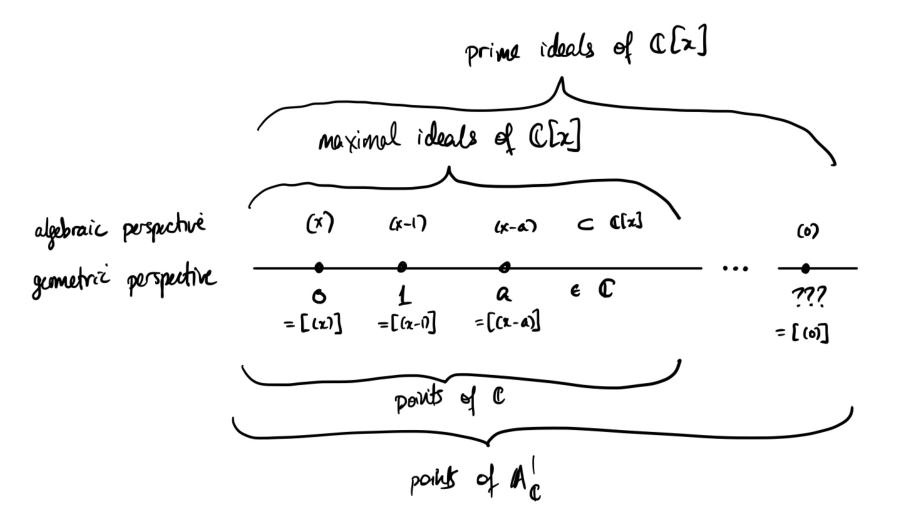
\includegraphics[width=\linewidth,height=\textheight,keepaspectratio]{Figures/complex affine line.png}
    				        \caption{The complex affine line $\A^1_{\bbC}$ (\cite{risingsea}, figure 3.1)}
    				        \label{fig: complex_affine_line}
    				    \end{figure}
    				This result generalises in an obvious manner to algebraically closed fields other than $\bbC$; so for instance, studying schemes over the field $\overline{\Q}$ of algebraic numbers might help one understand more about polynomials with rational coefficients.
    				\item \textbf{(The affine line over a separably closed but not algebraically closed field):} Let $k$ be a field that is separably closed but not algebraically closed (we can take $k = \F_p(t)^{\sep}$, for example). Then, the set of non-zero prime ideals of $\A^1_k$ need not be in bijection with $k$ itself.
    				\item \textbf{(Spectrum of the integers):} The prime ideals of $\Z$ are either generated by prime numbers themselves, or the zero ideal $(0)$. Thus, the set $\Spec \Z$ is in bijection with the \textit{union} of the set of all prime numbers and the set $\{(0)\}$. 
                \end{enumerate}
            \end{example}
        
        \subsubsection{The Zariski topology as a point-set topology} \index{Topology!Zariski}
            \begin{definition}[Zariski-closed subsets] \label{def: zariski_closed}
                Let $R$ be a commutative ring and let $\calF$ be an arbitrary subset of $R$. Then, let us declare that sets of the following form are closed in the to-be Zariski topology:
                    $$V(\calF) := \left\{\p \in \Spec R \mid \p \supset \calF \right\}$$
                When it might be possible to confuse Zariski-closed subsets of different ring spectra, we will write $V_R(\calF)$ instead of simply $V(\calF)$.
            \end{definition}
            \begin{remark}
                Of course, sets of the form $\Spec R \setminus V(\calF)$ are Zariski-open (that is, if we are assuming that the \href{https://ncatlab.org/nlab/show/excluded+middle}{\underline{the Law of Excluded Middle}} holds).
            \end{remark}
            
            \begin{proposition}[Well-definiteness of the Zariski topology] \label{prop: zariski_closed_well_definiteness}
                Let $R$ be an arbitrary commutative ring and assume the Law of Excluded Middle. Then, Zariski-closed subsets as defined in \ref{def: zariski_closed} actually define a topology on $\Spec R$, which of course, is called the Zariski topology.
            \end{proposition}
                \begin{proof}
                    For each subset $\calF$ of $R$, let us write $I(\calF)$ for the $R$-ideal generated by $\calF$. Let us now verify the axioms defining topologies on sets one-by-one.
                        \begin{enumerate}
                            \item \textbf{(The empty set and the whole set are closed):} The empty set is just $V(R)$ and that $\Spec R$ is just $V\left((0)\right)$, which are, by definition, closed in the Zariski topology. Thus, both the empty set and the whole space are Zariski-closed.
                            \item \textbf{(Finite unions of closed sets are closed):} Let $\{V(\calF_{\alpha})\}_{\alpha \in A}$ be a \textit{finite} set of Zariski-closed subsets of $\Spec R$ and consider the following chain of logical \textit{implications} (wherein $\p$ is a prime ideal of $R$, even though this fact can be inferred from the statements themselves):
                                $$
                                    \begin{aligned}
                                        & \p \in \bigcup_{\alpha \in A} V(\calF_{\alpha})
                                        \\
                                        \iff & \exists \alpha \in A: \p \in V(\calF_{\alpha})
                                        \\
                                        \iff & \exists \alpha \in A: \p \supset \calF_{\alpha}
                                        \\
                                        \iff & \bigvee_{\alpha \in A} (\p \supset \calF_{\alpha})
                                        \\
                                        \implies & \forall \left(f_{\alpha}\right)_{\alpha \in A} \in \prod_{\alpha \in A} \calF_{\alpha}: \prod_{\alpha \in A} f_{\alpha} \in \p
                                        \\
                                        \iff & \bigwedge_{\left(f_{\alpha}\right)_{\alpha \in A} \in \prod_{\alpha \in A} \calF_{\alpha}} \left(\prod_{\alpha \in A} f_{\alpha} \in \p\right)
                                        \\
                                        \iff & \p \supset \left\{\prod_{\alpha \in A} f_{\alpha} \: \bigg| \: \forall \alpha \in A: f_{\alpha} \in \calF_{\alpha} \right\}
                                        \\
                                        \iff & \p \in V\left(\left\{\prod_{\alpha \in A} f_{\alpha} \: \bigg| \: \forall \alpha \in A: f_{\alpha} \in \calF_{\alpha} \right\}\right)
                                    \end{aligned}
                                $$
                            wherein the fourth line, in particular, holds due to the fact that ideals, by definition, are closed under scalar multiplication by elements of their ambient rings. Now, to upgrade the fourth line to an equivalence, we can show that:
                                $$\bigwedge_{\left(f_{\alpha}\right)_{\alpha \in A} \in \prod_{\alpha \in A} \calF_{\alpha}} \left(\prod_{\alpha \in A} f_{\alpha} \in \p\right) \implies \bigvee_{\alpha \in A} (\p \supset \calF_{\alpha})$$
                            or, as we have assumed that the Law of Excluded Middle holds, we have the following:
                                $$
                                    \begin{aligned}
                                        & \left(\bigwedge_{\left(f_{\alpha}\right)_{\alpha \in A} \in \prod_{\alpha \in A} \calF_{\alpha}} \left(\prod_{\alpha \in A} f_{\alpha} \in \p\right) \implies \bigvee_{\alpha \in A} (\p \supset \calF_{\alpha})\right)
                                        \\
                                        \vdash & \left(\neg \bigwedge_{\left(f_{\alpha}\right)_{\alpha \in A} \in \prod_{\alpha \in A} \calF_{\alpha}} \left(\prod_{\alpha \in A} f_{\alpha} \in \p\right) \implies  \neg \bigvee_{\alpha \in A} (\p \supset \calF_{\alpha})\right)
                                    \end{aligned}
                                $$
                            meaning that we can prove the contraposition instead. To that end, consider the following:
                                $$
                                    \begin{aligned}
                                        & \neg \bigwedge_{\left(f_{\alpha}\right)_{\alpha \in A} \in \prod_{\alpha \in A} \calF_{\alpha}} \left(\p \ni \prod_{\alpha \in A} f_{\alpha}\right)
                                        \\
                                        \implies & \bigvee_{\left(f_{\alpha}\right)_{\alpha \in A} \in \prod_{\alpha \in A} \calF_{\alpha}} \neg \left(\p \ni \prod_{\alpha \in A} f_{\alpha}\right)
                                        \\
                                        \implies & \bigwedge_{\alpha \in A} \left(\bigvee_{f_{\alpha} \in \calF_{\alpha}} \neg(\p \ni f_{\alpha})\right)
                                        \\
                                        \implies & \bigwedge_{\alpha \in A} \left(\neg \bigwedge_{f_{\alpha} \in \calF_{\alpha}} (\p \ni f_{\alpha})\right)
                                        \\
                                        \implies & \bigwedge_{\alpha \in A} \neg (\p \supset \calF_{\alpha})
                                        \\
                                        \implies & \neg \bigvee_{\alpha \in A} (\p \supset \calF_{\alpha})
                                    \end{aligned}
                                $$
                            Thus, we have managed to show that:
                                $$\neg \bigwedge_{\left(f_{\alpha}\right)_{\alpha \in A} \in \prod_{\alpha \in A} \calF_{\alpha}} \left(\prod_{\alpha \in A} f_{\alpha} \in \p\right) \implies  \neg \bigvee_{\alpha \in A} (\p \supset \calF_{\alpha})$$
                            and therefore:
                                $$\p \in \bigcup_{\alpha \in A} V(\calF_{\alpha}) \iff \p \in V\left(\left\{\prod_{\alpha \in A} f_{\alpha} \: \bigg| \: \forall \alpha \in A: f_{\alpha} \in \calF_{\alpha} \right\}\right)$$
                            Because $\p$ was chosen arbitrarily, this implies that:
                                $$\bigcup_{\alpha \in A} V(\calF_{\alpha}) = V\left(\left\{\prod_{\alpha \in A} f_{\alpha} \: \bigg| \: \forall \alpha \in A: f_{\alpha} \in \calF_{\alpha} \right\}\right)$$
                            Hence, the \textit{finite} union $\bigcup_{\alpha \in A} V(\calF_{\alpha})$ is Zariski-closed by definition, and consequently, all finite unions of Zariski-closed sets are closed in the Zariski topology themselves (since $\{\calF_{\alpha}\}_{\alpha \in A}$ is an arbitrary fintie set of subsets of $R$). Note that the finiteness assumption on the index set $A$ is crucial, as without it, one would not be able to properly make sense of the product $\prod_{\alpha \in A} f_{\alpha}$.
                            \item \textbf{(Intersections of closed sets are closed):} Let $\{V(\calF_{\alpha})\}_{\alpha \in A}$ be an \textit{arbitrary} set of Zariski-closed subsets of $\Spec R$ and consider the following chain of logical equivalences (wherein $\p$ is a prime ideal of $R$, and again, this fact can be deduced from the statements themselves):
                                $$
                                    \begin{aligned}
                                        & \p \in \bigcap_{\alpha \in A} V(\calF_{\alpha})
                                        \\
                                        \iff & \forall \alpha \in A: \p \in V(\calF_{\alpha})
                                        \\
                                        \iff & \forall \alpha \in A: \p \supset \calF_{\alpha}
                                        \\
                                        \iff & \p \supset I\left(\bigcup_{\alpha \in A} \calF_{\alpha}\right)
                                        \\
                                        \iff & \p \in V\left(I\left(\bigcup_{\alpha \in A} \calF_{\alpha}\right)\right)
                                    \end{aligned}
                                $$
                            It tells us that \textit{any} prime ideal $\p$ is in an intersection of Zariski-closed subsets of $\Spec R$ defined by subsets $\calF_{\alpha}$ of $R$ if and only if it is in the Zariski-closed subset of $\Spec R$ defined by the ideal generated by the union of the sets $\calF_{\alpha}$, or in other words, that:
                                $$\bigcap_{\alpha \in A} V(\calF_{\alpha}) = V\left(I\left(\bigcup_{\alpha \in A} \calF_{\alpha}\right)\right)$$
                            In turn, this implies that the intersection of the Zariski-closed sets $V(\calF_{\alpha})$ is itself closed in the Zariski topology, and since the index set $A$ is was chosen arbitrarily, this means that arbitrary intersections of Zariski-closed sets are themselves Zariski-closed.
                        \end{enumerate}
                    Thus, with closed sets as in definition \ref{def: zariski_closed}, the Zariski topology on prime spectra of commutative rings is well-defined.
                \end{proof}
            \begin{corollary}[Quotients are closed] \label{coro: quotients_are_closed}
                Let $R$ be a commutative ring and let $I$ be an $R$-ideal. Then, $\Spec R/I$ is homeomorphic to a Zariski-closed subset of $\Spec R$. 
            \end{corollary}
                \begin{proof}
                    This comes from a straightforward application of the third isomorphism theorem for modules.
                \end{proof}
                
            \begin{definition}[A different approach: Zariski-open sets] \label{def: zariski_open}
                Let $R$ be a commutative ring. Then, let us declare that subsets of $\Spec R$ of the following form are open in the to-be Zariski topology:
                    $$D(f) := \{\p \in \Spec R \mid \p \not \ni f\}$$
                Whenever referring to more than one ring spectra, it might be beneficial to specifically write $D_R(f)$ instead of $D(f)$.
            \end{definition}
            \begin{remark} \label{remark: basic_opens_complements}
                For any commutative ring $R$, one can show through the following logical equivalences that:
                    $$D(f) = \Spec R \setminus V\left((f)\right)$$
                wherein $\p$ is an arbitrary prime ideal of $R$:
                    $$
                        \begin{aligned}
                            & \p \in D(f)
                            \\
                            \iff & \p \in \{\q \in \Spec R \mid \q \not \ni f\}
                            \\
                            \iff & \neg(\p \ni f)
                            \\
                            \iff & \neg(\p \supset (f))
                            \\
                            \iff & \p \in \Spec R \setminus \{\q \in \Spec R \mid \q \supset (f)\}
                            \\
                            \iff & \p \in \Spec R \setminus V\left((f)\right)
                        \end{aligned}
                    $$
            \end{remark}
            
            \begin{proposition}[Well-definiteness of the Zariski topology] \label{prop: zariski_open_well_definiteness}
                Let $R$ be an arbitrary commutative ring and assume the Law of Excluded Middle. Then, Zariski-open subsets as defined in \ref{def: zariski_open} actually define a topology on $\Spec R$, which of course, is called the Zariski topology.
            \end{proposition}
                \begin{proof}
                    Let us verify the axioms defining topologies on sets one-by-one.
                        \begin{enumerate}
                            \item \textbf{(The empty set and the whole set are open):} Consider the set $D(1)$, which by definition, is given by:
                                $$D(1) := \{\p \in \Spec R \mid \p \not \ni 1\}$$
                            Because prime ideals are defined to be proper, and because proper ideals are never (multiplicatively) unital, one gets that:
                                $$D(1) = \Spec R$$
                            In other words, the whole of $\Spec R$ is open by definition. Now, consider the following:
                                $$D(0) := \{\p \in \Spec R \mid \p \not \ni 0\} = \varnothing$$
                            which holds because ideals are submodules of their ambient rings, and modules over rings must contain $0$ (as an additive identity) by definition. Thus, the empty set is also Zariski-open by definition. 
                            \item \textbf{(Unions of open sets are open):} Let $\{f_{\alpha}\}_{\alpha \in A}$ be an \textit{arbitrary} set of elements of $R$ and let us apply remark \ref{remark: basic_opens_complements} to get the following chain of logical equivalences regarding the union of the sets $D(f_{\alpha})$, wherein $\p$ is an \textit{arbitrary} prime ideal of $R$:
                                $$
                                    \begin{aligned}
                                        & \p \in \bigcup_{\alpha \in A} D(f_{\alpha})
                                        \\
                                        \iff & \bigvee_{\alpha \in A} \left(\p \in D(f_{\alpha})\right)
                                        \\
                                        \iff & \bigvee_{\alpha \in A} \neg \left(\p \in V\left((f_{\alpha})\right)\right)
                                        \\
                                        \iff & \neg \bigwedge_{\alpha \in A} \left(\p \in V\left((f_{\alpha})\right)\right)
                                        \\
                                        \iff & \p \in \Spec R \setminus \bigcap_{\alpha \in A} V\left((f_{\alpha})\right)
                                    \end{aligned}
                                $$
                            This shows that:
                                $$\bigcup_{\alpha \in A} D(f_{\alpha}) = \Spec R \setminus \bigcap_{\alpha \in A} V\left((f_{\alpha})\right)$$
                            In proposition \ref{prop: zariski_closed_well_definiteness}, we have already shown using only definition \ref{def: zariski_closed} that arbitrary intersections of Zariski-closed sets are Zariski-closed themselves; in particular, this means that $\bigcap_{\alpha \in A} V\left((f_{\alpha})\right)$ is Zariski-closed. Then, by using the Law of Excluded Middle, one can see that the complement $\Spec R \setminus \bigcap_{\alpha \in A} V\left((f_{\alpha})\right)$ is necessarily Zariski-open. Thus, arbitrary unions of Zariski-open sets are Zariski-open themselves.
                            \item \textbf{(Finite intersections of open sets are open):} Let $\{f_{\alpha}\}_{\alpha \in A}$ be an \textit{finite} set of elements of $R$ and consider the following chain of logical equivalences regarding the union of the sets $D(f_{\alpha})$, wherein $\p$ is a prime ideal of $R$:
                                $$
                                    \begin{aligned}
                                        & \neg \left(\p \in \bigcap_{\alpha \in A} D(f_{\alpha})\right)
                                        \\
                                        \iff & \neg \bigwedge_{\alpha \in A} \left(\p \in D(f_{\alpha})\right)
                                        \\
                                        \iff & \bigvee_{\alpha \in A} \neg \left(\p \in D(f_{\alpha})\right)
                                        \\
                                        \iff & \bigvee_{\alpha \in A} \left(\p \in \Spec R \setminus D(f_{\alpha})\right)
                                        \\
                                        \iff & \bigvee_{\alpha \in A} \left(\p \in V\left((f_{\alpha})\right)\right)
                                        \\
                                        \iff & \p \in \bigcup_{\alpha \in A} V\left((f_{\alpha})\right)
                                    \end{aligned}
                                $$
                            (let us note that the fifth line holds thanks to remark \ref{remark: basic_opens_complements}). Now, the contraposition of the equivalence:
                                $$\neg \left(\p \in \bigcap_{\alpha \in A} D(f_{\alpha})\right) \iff \p \in \bigcup_{\alpha \in A} V\left((f_{\alpha})\right)$$
                            is:
                                $$\neg \neg \left(\p \in \bigcap_{\alpha \in A} D(f_{\alpha})\right) \iff \neg \left(\p \in \bigcup_{\alpha \in A} V\left((f_{\alpha})\right) \right)$$
                            From this, one gets the following proof:
                                $$
                                    \begin{aligned}
                                        & \neg \neg \left(\p \in \bigcap_{\alpha \in A} D(f_{\alpha})\right) \iff \neg \left(\p \in \bigcup_{\alpha \in A} V\left((f_{\alpha})\right) \right)
                                        \\
                                        \vdash & \left(\p \in \bigcap_{\alpha \in A} D(f_{\alpha})\right) \iff \left(\p \in \Spec R \setminus \bigcup_{\alpha \in A} V\left((f_{\alpha})\right) \right) 
                                        \\
                                        \vdash & \left(\bigcap_{\alpha \in A} D(f_{\alpha}) = \Spec R \setminus \bigcup_{\alpha \in A} V\left((f_{\alpha})\right)\right)
                                    \end{aligned}
                                $$
                            Lastly, let us recall that by \ref{prop: zariski_closed_well_definiteness}, the \textit{finite} union $\bigcup_{\alpha \in A} V\left((f_{\alpha})\right)$ of Zariski-closed sets is Zariski-closed itself, meaning that by the Law of Excluded Middle, the complement $\Spec R \setminus \bigcup_{\alpha \in A} V\left((f_{\alpha})\right)$ must be Zariski-open. Thus, the union $\bigcap_{\alpha \in A} D(f_{\alpha})$ is Zariski-open. Note that the finiteness assumption on the index set $A$ is crucial, as otherwise, the union $\bigcup_{\alpha \in A} V\left((f_{\alpha})\right)$ might not be Zariski-closed.
                        \end{enumerate}
                    Thus, with open sets as in definition \ref{def: zariski_open}, the Zariski topology on prime spectra of commutative rings is well-defined.
                \end{proof}
            
            \begin{proposition}[Unifying the two definitions] \label{prop: zariski_topology_equivalence}
                By asuming the Law of Excluded Middle, one gets the same topology on spectra of commutative rings via the approaches presented in definitions \ref{def: zariski_closed} and \ref{def: zariski_open}.
            \end{proposition}
                \begin{proof}
                    Let $R$ be a commutative ring. It is sufficient to show that for each element $f \in R$, the complement $\Spec R \setminus D(f)$ is closed in the sense of definition \ref{def: zariski_closed}, or equivalently, for each subset $\calF \subset R$, the complement $\Spec R \setminus V(\calF)$ is open in the sense of definition \ref{def: zariski_open}. We will be attempting the second approach. To that end, let us directly the following chain of logical equivalences:
                        $$
                            \begin{aligned}
                                & \p \in \bigcup_{\alpha \in A} D(f_{\alpha})
                                \\
                                \iff & \exists \alpha \in A: \p \in D(f_{\alpha})
                                \\
                                \iff & \exists \alpha \in A: \p \in \{\q \in \Spec R \mid \q \not \ni f_{\alpha}\}
                                \\
                                \iff & \exists \alpha \in A: \p \not \ni f_{\alpha}
                                \\
                                \iff & \bigvee_{\alpha \in A} \neg\left(\p \ni f_{\alpha}\right)
                                \\
                                \iff & \neg \bigwedge_{\alpha \in A} (\p \ni f_{\alpha}) 
                                \\
                                \iff & \neg \left(\p \supset \bigcup_{\alpha \in A} \{f_{\alpha}\}\right)
                                \\
                                \iff & \neg \left(\p \supset \{f_{\alpha}\}_{\alpha \in A}\right)
                                \\
                                \iff & \p \in \Spec R \setminus \left\{\q \in \Spec R \mid \q \supset \{f_{\alpha}\}_{\alpha \in A}\right\}
                                \\
                                \iff & \p \in \Spec R \setminus V\left(\{f_{\alpha}\}_{\alpha \in A}\right)
                            \end{aligned}
                        $$
                    Thus:
                        $$\bigcup_{\alpha \in A} D(f_{\alpha}) = \Spec R \setminus V\left(\{f_{\alpha}\}_{\alpha \in A}\right)$$
                    i.e. the complement of the Zariski-closed set $V\left(\{f_{\alpha}\}_{\alpha \in A}\right)$ inside $\Spec R$ is a union of Zariski-open sets $D(f_{\alpha})$, which we know from proposition \ref{prop: zariski_open_well_definiteness} to be Zariski-open itself. As stated, this implies that definitions \ref{def: zariski_closed} and \ref{def: zariski_open} give us the same Zariski topology on prime spectra of commutative rings.
                \end{proof}
            \begin{corollary} \label{coro: zariski_basis}
                Let $R$ be a commutative ring and let $f$ denote elements of $R$. Then, the distinguished Zariski-open sets $D(f)$ form a base of the Zariski topology on $\Spec R$.
            \end{corollary}
                \begin{proof}
                    This is a direct consequence of the fact that complements of Zariski-closed sets are unions of Zariski-open sets of the form $D(f)$.
                \end{proof}
            
            We have managed to show that on each ring spectrum, there is a canonical topology, namely the Zariski topology. A naturaly follow-up question is thus: can we upgrade $\Spec$ to a functor whose domain is $\Top$ instead of $\Sets$ ? Luckily, the answer is yes, although we will need to do some work to show that this is the case. 
            \begin{proposition}[Continuous functions between spectra] \label{prop: continuous_functions_between_spectra}
                By equipping prime spectra of commutative rings with the Zariski topology (in either the sense of definition \ref{def: zariski_closed} or \ref{def: zariski_open}), one naturally gets a functor:
                    $$\Spec: \Cring^{\op} \to \Top$$
                assigning to commutative rings their respective Zariski topological spaces.
            \end{proposition}
                \begin{proof}
                    It will suffice to show that given any ring homomorphism $f: A \to B$, the induced map $\Spec f: \Spec B \to \Spec A$ is continuous, which we can do by showing that preimages of Zariski-open subsets of $\Spec A$ under $\Spec f$ are closed in $\Spec B$; in fact, we can restrict our attention to \textit{basic} open subsets of $\Spec A$ (i.e. subsets of the form $D_A(a)$, for some $a \in A$), as they form a basis for the Zariski topology on $\Spec A$. Let $D_A(a)$ be such a basic open set. It preimage under $\Spec f$ is thus the following subset of $\Spec B$:
                        $$(\Spec f)^{-1}\left(D_A(a)\right) = \{\q \in \Spec B \mid (\Spec f)(\q) \in D_A(a)\}$$
                    Writing out the definition of $D_A(a)$ (cf. definition \ref{def: zariski_open}) then gives the following chain of logical equivalences:
                        $$
                            \begin{aligned}
                                & \q \in (\Spec f)^{-1}\left(D_A(a)\right)
                                \\
                                \iff & (\Spec f)(\q) \in D_A(a)
                                \\
                                \iff & f^{-1}(\q) \in D_A(a)
                                \\
                                \iff & \neg(f^{-1}(\q) \ni a)
                                \\
                                \iff & \neg(\q \ni f(a))
                                \\
                                \iff & \q \in D_B(f(a))
                            \end{aligned}
                        $$
                    which proves that:
                        $$(\Spec f)^{-1}\left(D_A(a)\right) = D_B(f(a))$$
                    and because $D_B(f(a))$ is open by definition, so is the preimage $(\Spec f)^{-1}(D_A(a))$. As stated at the beginning, this implies that $\Spec f$ is a continuous function, and thus there exists a functor:
                        $$\Spec: \Cring^{\op} \to \Top$$
                    assigning commutative rings and homomorphisms between them to ring spectra equipped with the Zariski topology and continuous maps in between.
                \end{proof}
                
            \begin{example}[Topologically interesting ring spectra]
                \noindent
                \begin{enumerate}
                    \item \textbf{(The complex affine plane and complex affine $n$-spaces):}
                        \begin{figure}[H]
                            \centering
                            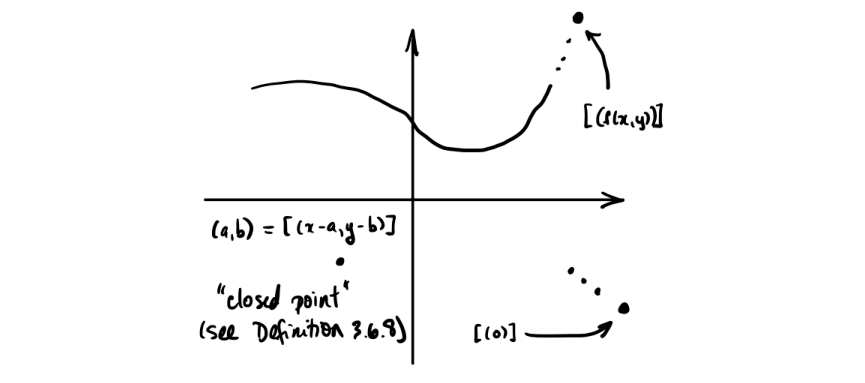
\includegraphics[width=\linewidth,height=\textheight,keepaspectratio]{Figures/complex affine plane.png}
                            \caption{The complex affine plane $\A^2_{\bbC}$ (\cite{risingsea}, figure 3.3)}
                            \label{fig: complex_affine_plane}
                        \end{figure}
                    \item \textbf{(Revisiting $\Spec \Z$):}
                        \begin{figure}[H]
                            \centering
                            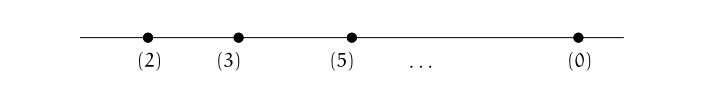
\includegraphics[width=\linewidth,height=\textheight,keepaspectratio]{Figures/Spec Z.png}
                            \caption{$\Spec \Z$ (\cite{risingsea}, figure 3.2)}
                            \label{fig: Spec_Z}
                        \end{figure}
                    \item \textbf{(A conic):}
                        \begin{figure}[H]
                            \centering
                            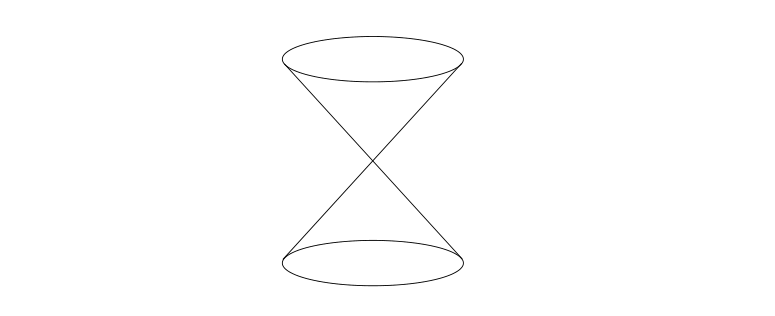
\includegraphics[width=\linewidth,height=\textheight,keepaspectratio]{Figures/conic.png}
                            \caption{A conic which is Zariski-closed inside $\A^3_{\bbC}$ (\cite{risingsea}, figure 3.4)}
                            \label{fig: conic}
                        \end{figure}
                \end{enumerate}
            \end{example}
            
            \begin{remark}[Comparing $\Spec$ and $\Spm$]
                Historically (and only because mathematicians were more interested in complex algebraic geometry back in the days), it was not the set of prime ideals of a commutative ring that was considered, but rather, the set of \textit{maximal} ideals. This was not out of \textit{na\"ivet\'e}, though. Maximal ideals enjoy being closed points in prime spectra of commutative rings (one can prove this by first looking at varieties $V(\m)$ associated to maximal ideals $\m$ of some commutative ring $R$, and then applying the definition of the (underlying set of) these varieties as spaces whose points are prime ideals containing $\m$, and then lastly, applying the usual definition of topological closures; as a corollary, one gets that prime ideals that are not maximal get sent by $\Spec$ to non-closed points in $\Spec R$), and so doing geometry with them is a lot more intuitive (albeit more restrictive as well) then doing so with all prime ideals. For instance, the underlying set of $\Spm \bbC[x]$ is precisely $\bbC$, whereas that of $\Spec \bbC[x]$ can be thought of as $\bbC \cup \{\infty\}$, i.e. as the Riemann sphere; in particular, the zero ideal $(0)$ corresponds to the point \say{at infinity}, which we denote by $\infty$. 
            \end{remark}
            
            \begin{example}[Non-isomorphic rings with homeomorphic spectra] \label{example: nonisomorphic_rings_with_the_same_spectra}
                The following examples are of non-isomorphic rings with homeomorphic prime spectra; through them, we are able to show that the functor $\Spec: \Cring^{\op} \to \Top$ is not an equivalence of categories (nor even a fully faithful inclusion). 
                \begin{enumerate}
                    \item \textbf{(Fields):} The prime spectra of any field is just the one-point space, but clearly, not all fields are isomorphic.
                    \item \textbf{(Discrete valuation rings):} The spectrum of any \href{https://en.wikipedia.org/wiki/Discrete_valuation_ring}{\underline{discrete valuation ring}} is homeomorphic to the \href{https://ncatlab.org/nlab/show/Sierpinski+space}{\underline{Sierpi\'nski space}} (to see why this is the case, firstly check that discrete valuation rings only have two prime ideals, one being the zero ideal and one being the unique maximal ideal, and that the latter is a closed point in the spectrum whereas the former is generic), but of course, not all discrete valuation rings are isomorphic to one another.
                \end{enumerate}
            \end{example}
        
        \subsubsection{Affine schemes}
            Next, we will be discussing the idea of so-call \textbf{structure sheaves}, but in order to make sense of these entities, we will need to know what $\C$-valued sheaves are for categories $\C$ more general than $\Sets$:
            \begin{definition}[$\C$-valued sheaves] \label{def: C_valued_sheaves}
                This definition is an adaptation of definition 2.6 in \cite{nlab:sheaf} so that our sheaves might take values in categories other than $\Sets$.
                \begin{enumerate}
                    \item \textbf{($\C$-valued sheaves):} Let $(\S, J)$ be a site\footnote{... which is not necessarily small, as cases such as $\S \cong \Top$ and $\S \cong \Mfd^{\smooth}_{/\R}$ are interesting in their own rights.} and let $\C$ be a category with \textit{enough small limits} and \textit{enough filtered colimits} (the purpose of the second hypothesis is to ensure that stalks, should they exist, are well-defined); note that $\C$ need not be small. Additionally, fix an \textit{arbitrary} object $x$ of $\S$ along with a covering sieve $\calU_{/x} \in J$ thereon. Also, let $j: \S \to \Psh_{\C}(\S)$ be the Yoneda embedding. Then, a \textbf{$\C$-valued sheaf} on $(\S, J)$ is a functor $\calF: \S^{\op} \to \C$ such that $\calF(x) \cong \calF\left( \underset{u \in \calU_{/x}}{\colim} ju \right)$.
                    \item \textbf{($\C$-topoi):} $\C$-valued sheaves on a given site $(\S, J)$ form a category in the obvious manner. We shall be writing $\Sh_{\C}(\S, J)$ for this category, and such categories will be called \textbf{$\C$-topoi}, even though this is an abuse of terminology.
                \end{enumerate}
            \end{definition}
            \begin{example}[Sheaves of rings]
                The notion of sheaves of rings, which subsumes that of structure sheaves (cf. proposition \ref{prop: structure_sheaf}), follows suite from definition \ref{def: C_valued_sheaves}. Note that such constructions are well-defined, as the category of rings is both complete and cocomplete.
            \end{example}
            
            Having defined sheaves that might take values categories other than $\Sets$, let us now try to define affine schemes as locally ringed spaces whose underlying topological spaces are spectra of commutative rings, and whose structure presheaves have a certain condition imposed upon them, which happens to guarantee that:
                \begin{enumerate}
                    \item these structure presheaves are indeed sheaves (proposition \ref{prop: structure_sheaf}) with local stalks (corollary \ref{coro: structure_sheaf_properties}), and
                    \item they are unique (proposition \ref{prop: structure_sheaf_uniqueness}), which is an important feature, because ringed spaces are uniquely defined by their structure sheaves; this fact will also be used to establish the fully faithfulness of $\Spec$ as a functor from $\Cring^{\op}$ to the category $\Loc\Ringed\Spc$ of locally ringed spaces. 
                \end{enumerate}
            Our efforts will culminate in definition \ref{def: affine_schemes}.
                
            \begin{proposition}[Structure sheaves of affine schemes] \label{prop: structure_sheaf} \index{Structure sheaves}
                Let $k$ be a base commutative ring, and let $\calO_{\Spec R}$ be \textit{a} presheaf of commutative rings on $\Ouv(\Spec R)$ determined by the following rule on objects:
                    $$\calO_{\Spec R}(D_R(f)) \cong R_f$$
                for all element $f \in R$. Any presheaf on $\Ouv(\Spec R)$ that are defined this way is a Zariski sheaf (i.e. a sheaf on the site $\Ouv(\Spec R)$ of Zariski-open subsets of $\Spec R$), and is called \textit{a} \textbf{structure sheaf} on $\Spec R$.
            \end{proposition}
            \begin{corollary}[On the locality of stalks] \label{coro: structure_sheaf_properties}
                Let $R$ be a commutative ring and let $\p$ be an arbitrary prime ideal of $R$. Then one has the following characterisation of the stalk $\calO_{\Spec R, \p}$ at $\p$ of the structure sheaf $\calO_{\Spec R}$:
                    $$\calO_{\Spec R, \p} \cong R_{\p}$$
                This shows that affine schemes are, in fact, \textit{locally} ringed spaces and not just ringed spaces. 
            \end{corollary} 
                \begin{proof}
                    Recall that the stalk $\calF_x$ of a sheaf (of sets) $\calF$ on a topological space $(X, \Ouv(X))$ is given by the filtered colimit indexed by the poset of open neighbourhoods of the chosen point $x \in X$:
                        $$\calF_x \cong \underset{U \in \{V \in \Ouv(X) \mid V \ni x\}}{\colim} \calF(U)$$
                    By adapting this definition to the underlying Zariski-topological spaces of affine schemes, we get that:
                        $$\calO_{\Spec R, \p} \cong \underset{U \in \{V \in \Ouv(\Spec R) \mid V \ni \p\}}{\colim} \calO_{\Spec R}(U)$$
                    with $\Ouv(\Spec R)$ the Zariski topology defined via open sets as in definition \ref{def: zariski_open}. In corollary \ref{coro: zariski_basis}, we have already seen how the distinguished Zariski-open sets defined in definition \ref{def: zariski_open} form a basis for the Zariski topology on commutative ring spectra, and so the above filtered colimit can be rewritten as:
                        $$\calO_{\Spec R, \p} \cong \underset{D_R(f) \in \{V \in \Ouv(\Spec R) \mid V \ni \p\}}{\colim} \calO_{\Spec R}\left(D_R(f)\right)$$
                    and because $D_R(f) = \{\p \in \Spec R \mid \p \not \ni f\}$, one subsequently gets:
                        $$\calO_{\Spec R, \p} \cong \underset{f \in \{g \in R \mid g \not \in \p\}}{\colim} \calO_{\Spec R}\left(D_R(f)\}\right)$$
                    Lastly we have the following isomorphism:
                        $$\calO_{\Spec R, \p} \cong \underset{f \in \{g \in R \mid g \not \in \p\}}{\colim} \calO_{\Spec R}\left(D_R(f)\right) \cong \underset{f \in R \setminus \p}{\colim} R_f \cong R_{\p}$$
                    Thus $\calO_{\Spec R, \p} \cong R_{\p}$ as claimed.
                \end{proof}
                
            \begin{proposition}[Uniqueness of structure sheaves] \label{prop: structure_sheaf_uniqueness}
                Let $R$ be a commutative ring. Then, there is only one unique structure sheaf attached to $\Spec R$. 
            \end{proposition}
                \begin{proof}
                    Suppose to the contrary that there exist two \textit{distinct} Zariski sheaves of $R$-algebras on ${}^{R/}\Comm\Alg^{\op}$ $\calF$ and $\calG$ such that:
                        $$\forall f \in R: \calF(\Spec R_f) \cong \calG(\Spec R_f) \cong R_f$$
                    However, the localisation of any commutative at its multiplicative identity is just itself, and so:
                        $$\calF(\Spec R) \cong \calG(\Spec R) \cong R$$
                    for all commutative rings $R$. This means that the functors $\calF$ and $\calG$ are naturally isomorphic, i.e. they can not be distinct. Thus, the structure sheaf attached to a given ring spectrum is unique (up to natural isomorphisms, of course).
                \end{proof}
                
            \begin{example}[Spotting structure sheaves in the wild]
                Let $R$ be a discrete valuation ring that is a \href{https://en.wikipedia.org/wiki/Dedekind_domain}{\underline{Dedekind domain}} (so the only proper ideals of $R$ would be $(0)$ and its unique maximal ideal) with unique maximal ideal $\p$, and recall that its spectrum is (homeomorphic to) the Sierpi\'nski space (see example \ref{example: nonisomorphic_rings_with_the_same_spectra} for more details); in particular, the subset $\{(0)\}$ of $\Spec R = \{(0), \p\}$ is the only non-empty open proper subset. Now, suppose that $\calF$ is a Zariski sheaf on $\Spec R$ given by the following formula:
                    $$
                        \calF(U) \cong 
                        \begin{cases}
                            \text{$R$ if $U = \Spec R$}
                            \\
                            \text{$\Frac R$ if $U = \{(0)\}$}
                        \end{cases}
                    $$
                (note that discrete valuation rings are integral domains, so it makes sense to consider their fields of fractions). The point that is to be made here is that $\calF$ qualifies as a structure sheaf on $\Spec R$. To see why this is the case, note that because $R$ has only two prime ideals, namely $(0)$ and $\p$, 
            \end{example}
            
            \begin{example}[The complex affine line]
                Recall that in example \ref{example: spectra_sets}, we have seen how a point of the complex affine line $\A^1_{\bbC}$ is either the zero ideal, or of the form $(t - a)$ for any complex number $a$; one should keep the following picture in mind:
                    \begin{figure}[H]
				        \centering
				        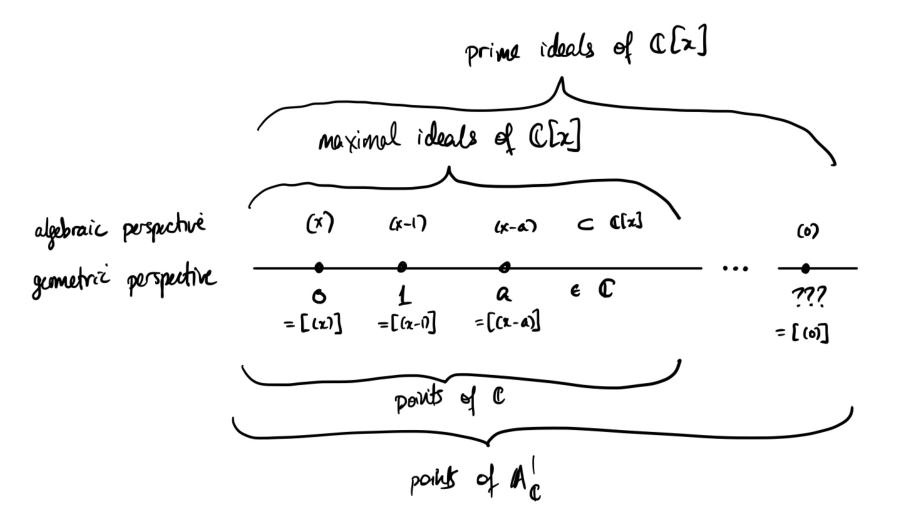
\includegraphics[width=\linewidth,height=\textheight,keepaspectratio]{Figures/complex affine line.png}
				        \caption{The complex affine line $\A^1_{\bbC}$ (\cite{risingsea}, figure 3.1)}
				        \label{fig: complex_affine_line_stalks}
				    \end{figure}
			    \noindent
			    Now, as an affine scheme, $\A^1_{\bbC}$ comes equipped with a structure sheaf $\calO_{\A^1_{\bbC}}$, whose stalks, as shown in corollary \ref{coro: structure_sheaf_properties}, are precisely the localisations of $\bbC[t]$ at its prime ideals. There are thus two cases:
			        \begin{enumerate}
			            \item The stalk at $(0)$ is given by:
			                $$\calO_{\A^1_{\bbC}, (0)} \cong \bbC[t]_{(0)} \cong \bbC(t)$$
		                and thus the residue field is trivially $\bbC(t)$.
			            \item At non-zero primes, the stalks of the structure sheaf $\calO_{\A^1_{\bbC}}$ are given by the following localisations:
			                $$\calO_{\A^1_{\bbC}, (t - a)} \cong \bbC[t]_{(t - a)}$$
		                whose elements we note to be fractions of the form $\frac{f(t)}{g(t)}$ whose denominators do not vanish at $t = a$. Now, recall that the localisation of any commutative ring at a prime ideal is a local ring, and that inside \textit{any} local commutative ring, elements in the complement of the unique maximal ideal are units; in particular, these facts imply that the elements of the complement $\bbC[t]_{(t - a)} \setminus (t - a)\bbC[t]_{(t - a)}$ are all invertible. Consequently, these elements must be fractions $\frac{f(t)}{g(t)}$ whose numerators and denominators both do not vanish at $t = a$. Thus, a reasonable description of the canonical quotient map is the evaluation map:
		                    $$\frac{f(t)}{g(t)} \mapsto \frac{f(a)}{g(a)}$$
	                    whose image is precisely $\bbC$. Therefore, the stalks of $\calO_{\A^1_{\bbC}}$ are all isomorphic to $\bbC$.
			        \end{enumerate}
            \end{example}
        
            \begin{definition}[Affine schemes] \label{def: affine_schemes}
                An \textbf{affine scheme} is a locally ringed space that is isomorphic to one of the form $(|\Spec R|, \calO_{\Spec R})$ for some commutative ring $R$. Morphisms of affine schemes are morphisms of locally ringed spaces, and as such, one has a full subcategory $\Sch^{\aff}$ of affine schemes within the category of locally ringed spaces. 
            \end{definition}
            
            \begin{theorem}[Isbell Duality for locally ringed spaces] \label{theorem: isbell_duality_for_locally_ringed_spaces}
                There is an adjunction as follows:
                    $$
                        \begin{tikzcd}
                        	{\Cring^{\op}} & \Loc\Ringed\Spc
                        	\arrow[""{name=0, anchor=center, inner sep=0}, "\Spec"', bend right, from=1-1, to=1-2]
                        	\arrow[""{name=1, anchor=center, inner sep=0}, "\Gamma"', bend right, from=1-2, to=1-1]
                        	\arrow["\dashv"{anchor=center, rotate=-90}, draw=none, from=1, to=0]
                        \end{tikzcd}
                    $$
            \end{theorem}
            \begin{corollary}
                The adjunction from theorem \ref{theorem: isbell_duality_for_locally_ringed_spaces} restricts down to an adjoint equivalence $\Sch^{\aff} \cong \Cring^{\op}$.
            \end{corollary}

    \subsection{The category of schemes}
        \subsubsection{Schemes}
            \begin{definition}[Schemes] \label{def: schemes}
                A \textbf{scheme} is a locally ringed space $(|X|, \calO_X)$ such that every point $x \in |X|$ as a Zariski-open neighbourhood $U_x \ni x$ that is isomorphic to an affine scheme. Morphisms of schemes are nothing but morphisms of locally ringed spaces, meaning that schemes form a category $\Sch$ which embeds fully faithfully into the category of locally ringed spaces.
            \end{definition}
            
            \begin{proposition}[Open subschemes are open locally ringed subspaces] \label{prop: open_subschemes_are_open_locally_ringed_subspaces}
                Let $X$ be a scheme and let $U \subseteq X$ be an open locally ringed subspace. Then, $U$ will be an open subscheme of $X$. 
            \end{proposition}
                \begin{proof}
                    
                \end{proof}
            \begin{corollary}[Zariski-bases of schemes] \label{coro: zariski_bases_of_schemes}
                
            \end{corollary}
    
        \subsubsection{Properties of schemes and their morphisms}
        
        \subsubsection{Topologies on schemes}
    
    \subsection{Varieties}

    \subsection{Cohomology of schemes and derived categories of coherent sheaves}
    
    \section{Algebraic spaces}
    
    \section{Algebraic stacks}
	    
	    %\chapter{Derived schemes} \label{chapter: cohomology_and_derived_schemes}
    \begin{abstract}
        
    \end{abstract}
    
    \minitoc
    
    \section{Sheaf cohmology}
        \subsection{Vanishing theorems}
            \subsubsection{Quasi-coherent sheaves and Serre's affineness criterion}
            
            \subsubsection{Higher direct images}
        
        \subsection{Base change}
        
        \subsection{Cohomology of projective varieties}
        
        \subsection{Some useful theorems}
            \subsubsection{Theorems on duality}
            
            \subsubsection{The theorem on formal functions}
            
            \subsubsection{The Grothendieck Existence Theorem; Algebraisation Theorems}

    \section{Derived schemes}
        \subsection{(Un)necessary \texorpdfstring{$\infty$}{}-categorical technicalities}
            \begin{convention}[Some typographical conventions]
                For the sake of linguistic simplicity (and since typing \say{$\infty$} gets very tedious very quickly), we shall refrain from specfifying the homotopicality of many $\infty$-categorical operations. For instance, $(\infty, 1)$-limits shall almost always be referred to simply as \say{limits}, and so on. Also, we shall only refer to $(\infty, 1)$-categories by their \say{full name}, so to say, when $(\infty, 2)$-categories are not around; otherwise, they shall simply be known as $\infty$-categories.
            \end{convention}
            
            \subsubsection{What on earth is an \texorpdfstring{$\infty$}{}-category ?}
        
            \subsubsection{\texorpdfstring{$\infty$}{}-topoi and \texorpdfstring{$\infty$}{}-stacks}
                \begin{remark}[Regular cardinals]
                    From now on we will be using the notion of regular cardinals often. For details on the notion, see definition \ref{def: limit_cardinal}.
                \end{remark}
            
                \begin{definition}[$\infty$-topoi] \label{def: infinity_topoi}
                    \noindent
                    \begin{enumerate}
                        \item \textbf{(Localisations of $\infty$-categories):} 
                            \begin{enumerate}
                                \item \textbf{(Reflexivity):} A \textit{fully faithful} $\infty$-functor:
                                    $$R: \C \to \D$$
                                identifies an $\infty$-category $\C$ as a \textbf{reflexive full $\infty$-subcategory} of another $\infty$-category $\D$ if it admits a left-$(\infty, 1)$-adjoint. Should this left-adjoint functor preserve all finite $(\infty, 1)$-limits, then the full faithful reflexive embedding $R: \C \to \D$ shall be called \textbf{exact}.
                                \item \textbf{(Localisations):} An $\infty$-functor:
                                    $$L: \D \to \C$$
                                is called a \textbf{localisation} if it admits a fully faithful right-$(\infty, 1)$-adjoint, which we note to necessarily be a reflexive embedding, by definition; we shall thus dub the right-adjoint component the \textbf{reflector}. Alternatively, one may characterise the \textbf{localisation} of an $\infty$-category $\D$ at a full $\infty$-subcategory $\C$ as an $(\infty, 1)$-adjoint pair:
                                    $$
                                        \begin{tikzcd}
                                        	\C & \D
                                        	\arrow[""{name=0, anchor=center, inner sep=0}, "L"', shift right=2, from=1-2, to=1-1]
                                        	\arrow[""{name=1, anchor=center, inner sep=0}, "R"', shift right=2, hook, from=1-1, to=1-2]
                                        	\arrow["\dashv"{anchor=center, rotate=-90}, draw=none, from=0, to=1]
                                        \end{tikzcd}
                                    $$
                                whose right-adjoint component is fully faithful. 
                                
                                A localisation that is \textit{exact} shall be called a \textbf{topological localisation}. 
                            \end{enumerate}
                        \item \textbf{(Accessibility and geometric embeddings/localisations):}
                            \begin{enumerate}
                                \item \textbf{(Accessibility):} Let $\kappa$ be some \href{https://ncatlab.org/nlab/show/regular+cardinal}{\underline{regular cardinal}}. An $\infty$-category $\C'$ is said to be \textbf{$\kappa$-accessible} if and only if it is equivalent to the $(\infty, 1)$-ind-completion of some $\kappa$-small $\infty$-category $\C$, i.e. one should be able to identify $\C'$ as a full $\infty$-subcategory of $\Psh_{(\infty, 1)}(\C)$ which is closed under all $\kappa$-small $(\infty, 1)$-filtered colimits.
                                \item \textbf{($(\infty, 1)$-geometric embeddings and $\infty$-topoi):} An \textbf{$\infty$-topos} \textit{\`a la} Rezk-Lurie is the topological localisation of some $\infty$-category of $(\infty, 1)$-presheaves at some \textit{accessible} full $\infty$-subcategory; the adjoint pair defining this localisation may either be referred to as an \textbf{$\infty$-geometric embedding} or an \textbf{$\infty$-geometric localisation}, depending on whether we wish to put emphasis on the left-adjoint or right-adjoint component.
                                
                                One very important thing to note is that every $(\infty, 1)$-presheaf $\infty$-category is trivially an $\infty$-topos; we refer to them as $(\infty, 1)$-presheaf $\infty$-topoi. 
                            \end{enumerate}
                    \end{enumerate}
                \end{definition}
                
                In algebraic geometry, one cares as much about sheaves as the topoi they span. Therefore, it would be nice if $\infty$-topoi were to behave as homotopical analogues of Grothendieck $1$-topoi (and let us recall that there is a geometric embedding from every Grothendieck $1$-topos into a presheaf $1$-topos), in that its objects could be realised as higher sheaves on higher sites. Luckily, such a characterisation of $\infty$-topos is available. We shall, however, need to roll our sleeves up a bit to obtain it.
                
                \begin{definition}[$\infty$-sites and $\infty$-descent theory] \label{def: infinity_sites}
                    \noindent
                    \begin{enumerate}
                        \item \textbf{($\infty$-coverages):} 
                            \begin{enumerate}
                                \item \textbf{($\infty$-sieves):} An $\infty$-sieve on an object $X$ of some $\infty$-category $\C$ is nothing more than an $(\infty, 1)$-subpresheaf of the representable presheaf $h_X$; i.e. for every test object $X_0$ of $\C_{/X}$ and every $\infty$-sieve $\U$ on $X$, one can identify $\U(X_0)$ as a full $\infty$-subcategory ($\infty$-subgroupoid, actually) of the $\infty$-groupoid $\C(X_0, X)$.
                                
                                An $\infty$-sieve $\U$ is said to \textbf{cover} an object $X$ of an $\infty$-category $\C$ if and only if $X$ is the $(\infty, 1)$-colimit of the \v{C}ech nerve $\U^{\bullet}_{/X}$. 
                                \item \textbf{(Axioms for $\infty$-coverages):} The following are conditions for a class of sieves on objects of some base $\infty$-category to qualify as an \textbf{$\infty$-coverage}:
                                    \begin{itemize}
                                        \item Representable $(\infty, 1)$-presheaves - viewed as $\infty$-sieves - cover the objects they represent.
                                        \item $(\infty, 1)$-pullbacks of covering $\infty$-sieves must also be covering $\infty$-sieves themselves. 
                                        \item Should the $(\infty, 1)$-pullback of an $\infty$-sieve be one that covers, then the first $\infty$-sieve must also be a covering $\infty$-sieve.
                                    \end{itemize}
                                An $\infty$-category equipped with an $\infty$-coverage is an \textbf{$\infty$-site.}
                            \end{enumerate}
                        \item \textbf{($\infty$-descent theory):} An $\infty$-prestack $\calY$ (cf. convention \ref{conv: infinity_prestacks}) on some $\infty$-category $\C$ equipped with an $\infty$-coverage $J$ (i.e. an $\infty$-site $(\C, J)$) is said to \textbf{satisfy $J$-descent} if and only if for all objects $X$ of $\C$ and for all $\infty$-sieves $\U$ that covers $X$, one has the following equivalence of $\infty$-groupoids:
                            $$\calY(X) \cong \calY\left((\infty, 1)\-\colim \U^{\bullet}_{/X}\right)$$
                        In particular, $(\infty, 1)$-presheaves that satisfy descent are \textbf{$(\infty, 1)$-sheaves}.
                    \end{enumerate}
                \end{definition}
                
                \begin{definition}[Presentability] \label{def: presentable_infinity_categories}
                    Let $\kappa$ be regular cardinal. Then, a $\kappa$-accessible $\infty$-category is said to be \textbf{$\kappa$-presentable} if it is furthermore $\kappa$-small $(\infty, 1)$-cocomplete. In other words, a $\kappa$-accessible $\infty$-category is a \textit{full} $\infty$-subcategory of the $(\infty, 1)$-presheaf $\infty$-topos over some underlying $\infty$-category that is \textit{closed under all $\kappa$-small $(\infty, 1)$-colimits}; clearly, every object in a $\kappa$-presentable category \textit{can be built out of a $\kappa$-small set of objects using $(\infty, 1)$-colimits}.
                \end{definition}
                \begin{example}[Examples of presentable $\infty$-categories]
                    
                \end{example}
                
                \begin{definition}[Universal $(\infty, 1)$-colimits] \label{def: universal_colimits}
                    Given any finitely $(\infty, 1)$-complete $\infty$-category $\E$, one can build so-called pullback $\infty$-functors:
                        $$f^*: \E_{/y} \to \E_{/x}$$
                    via $(\infty, 1)$-pullbacks along arrows $f: x \to y$. If a $(\infty, 1)$-colimit in $\E$ is preserved by all these pullback $\infty$-functors, then we shall call it \textbf{universal}.
                \end{definition}
                
                \begin{definition}[Subobject classifiers in $\infty$-categories] \label{def: subobject_classifiers}
                    \noindent
                    \begin{enumerate}
                        \item \textbf{(Monomorphisms):} A morphism:
                            $$f: x \to y$$
                        in an $\infty$-category $\E$ is a \textbf{monomorphism} if and only if $\E(x, -)$ is an $(\infty, 1)$-subfunctor of $\E(y, -)$: that is to say, for all test objects $x_0$ of $\E$, $\E(x, x_0)$ is a full $\infty$-subcategory of the $\infty$-groupoid $\E(y, x_0)$. 
                        \item \textbf{(Subobject classifiers):} Let $\E$ be a $(\infty, 1)$-complete $\infty$-category and let us denote its terminal object by $1$ (note that such a terminal object exists as a consequence of the finite-completeness hypothesis). Then, a morphism:
                            $$t: 1 \to \Omega$$
                        of $\E$ will be called a \textbf{subobject classifier} if and only if it is terminal in the (non-full) $\infty$-subcategory of the $\infty$-category $\E^{[1]} \cong \infty\-1-\Cat([1], \E)$ of arrows and commutative squares in $\E$ spanned by monomorphisms.
                        
                        Thanks to the assumption that $\E$ is finitely $(\infty, 1)$-complete, if a subobject classifier $t: 1 \to \Omega$ exists, one will be able to write any monomorphism $u \to x$ in $\E$ as the pullback of the subobject classifier along some \textit{unique} morphism $\chi_x: x \to \Omega$.
                    \end{enumerate}
                \end{definition}
                
                \begin{definition}[(De)looping] \label{def: looping} \index{Loop spaces} \index{Classifying spaces} 
                    \noindent
                    \begin{enumerate}
                        \item \textbf{(Loop spaces):} Let $\S$ be a finitely $(\infty, 1)$-complete $\infty$-category of \say{spaces} and let $X$ be some object thereof; also, let $*$ be a terminal object of $\S$. Then, the \textbf{loop space} $\loopspace X$ fits into the following $(\infty, 1)$-pullback square:
                            $$
                                \begin{tikzcd}
                                	{\loopspace X} & {*} \\
                                	{*} & X
                                	\arrow[from=1-1, to=2-1]
                                	\arrow[from=2-1, to=2-2]
                                	\arrow[from=1-1, to=1-2]
                                	\arrow[from=1-2, to=2-2]
                                	\arrow["\lrcorner"{anchor=center, pos=0.125}, draw=none, from=1-1, to=2-2]
                                \end{tikzcd}
                            $$
                        \item \textbf{(Classifying spaces):} Within the same framework, one can also define the so-called \textbf{classifying space} or \textbf{delooping space} of an object $H$ as the $(\infty, 1)$-pushout of the unique morphism $H \to *$ along itself:
                            $$
                                \begin{tikzcd}
                                	H & {*} \\
                                	{*} & {\bfB H}
                                	\arrow[from=1-1, to=2-1]
                                	\arrow[from=2-1, to=2-2]
                                	\arrow[from=1-1, to=1-2]
                                	\arrow[from=1-2, to=2-2]
                                	\arrow["\lrcorner"{anchor=center, pos=0.125, rotate=180}, draw=none, from=2-2, to=1-1]
                                \end{tikzcd}
                            $$
                        Note that because our ambient $\infty$-category is only finitely $(\infty, 1)$-complete, deloopings of its objects may or may not exist; should they do, however, they would guarantee the existence of all $(\infty, 1)$-coequalisers in $\E$ (we will use this fact in the proof of lemma \ref{lemma: building_infinity_topoi_out_of_colimits}).
                    \end{enumerate}
                    It is not too hard to see that:
                        $$\loopspace \bfB H \cong H$$
                    and if $(\infty, 1)$-pushouts were to exist in $\E$:
                        $$\bfB \loopspace X \cong X$$
                \end{definition}
                \begin{example}
                    \noindent
                    \begin{enumerate}
                        \item \textbf{((De)looping of spheres):} The simplest setting in which one can perform (de)looping on objects of a finitely $(\infty, 1)$-complete $\infty$-category is when $\S$ is the homotopy category $\Ho\Top$ of the category $\Top$ of topological spaces, which happens to be $(\infty, 1)$-cocomplete. For instance, for all positive integers $n$, the loop space of the $(n + 1)$-sphere is nothing but the $n$-sphere:
                            $$
                                \begin{tikzcd}
                                	{\bbS^n} & {*} \\
                                	{*} & {\bbS^{n + 1}}
                                	\arrow[from=1-1, to=2-1]
                                	\arrow[from=2-1, to=2-2]
                                	\arrow[from=1-1, to=1-2]
                                	\arrow[from=1-2, to=2-2]
                                	\arrow["\lrcorner"{anchor=center, pos=0.125, rotate=180}, draw=none, from=2-2, to=1-1]
                                \end{tikzcd}
                            $$
                        and conversely, the delooping of the $n$-sphere is the $(n + 1)$-sphere.
                        \item \textbf{(\v{C}ech nerves):} The delooping of the \v{C}ech nerve $u^{\bullet}_{/x}$ on some object $x$ of a finitely $(\infty, 1)$-complete $\infty$-category is exactly $x$. 
                    \end{enumerate}
                \end{example}
                
                \begin{lemma}[Building $\infty$-topoi out of colimits] \label{lemma: building_infinity_topoi_out_of_colimits}
                    Let $\kappa$ be a regular cardinal. Then, every $\kappa$-small $\infty$-topos is necessarily $\kappa$-presentable, has subobject classifiers, and the $(\infty, 1)$-colimits therein (which are all $\kappa$-small) are all universal.
                \end{lemma}
                    \begin{proof}
                        Fix a base $\kappa$-small $\infty$-category $\C$ and the following topological localisation defining an $\infty$-topos $\E$, which is necessarily $\kappa$-small by virtue of being a full $\infty$-subcategory of the $\kappa$-small $\infty$-category $\Psh_{(\infty, 1)}(\C)$:
                            $$
                                \begin{tikzcd}
                                	\E & {\Psh_{(\infty, 1)}(\C)}
                                	\arrow[""{name=0, anchor=center, inner sep=0}, "L"', shift right=2, from=1-2, to=1-1]
                                	\arrow[""{name=1, anchor=center, inner sep=0}, "R"', shift right=2, hook, from=1-1, to=1-2]
                                	\arrow["\dashv"{anchor=center, rotate=-90}, draw=none, from=0, to=1]
                                \end{tikzcd}
                            $$
                        \begin{enumerate}
                            \item \textbf{(Presentability):} Because $\kappa$-small $\infty$-topos are already $\kappa$-accessible by default (cf. definition \ref{def: infinity_topoi}), it shall suffice to show that they are $\kappa$-small $(\infty, 1)$-cocomplete. For this, we shall attempt to show that $\E$ has all $(\infty, 1)$-coproducts and all $(\infty, 1)$-coequalisers. 
                                \begin{enumerate}
                                    \item \textbf{(Coproducts):} By viewing our accessible $\infty$-category $\E$ as a quasi-category (which in particular, have underlying topological spaces), we can simply apply the Seifert-van Kampen Theorem to see how $(\infty, 1)$-coproducts ought to exist in $\E$ via the existence of liftings inside pushout squares of the following form: 
                                        $$
                                            \begin{tikzcd}
                                            	\varnothing & \bullet \\
                                            	\bullet & \bullet
                                            	\arrow[from=1-1, to=2-1]
                                            	\arrow[from=2-1, to=2-2]
                                            	\arrow[from=1-1, to=1-2]
                                            	\arrow[from=1-2, to=2-2]
                                            	\arrow[dashed, from=2-1, to=1-2]
                                            	\arrow["\lrcorner"{anchor=center, pos=0.125, rotate=180}, draw=none, from=2-2, to=1-1]
                                            \end{tikzcd}
                                        $$
                                    These liftings exist thanks to the fact that topological spaces have underlying sets, and one can always order their cardinalities. One thing to note here is that the Seifert-van Kampen Theorem can be applied here because disjoint spaces intersect at the empty set (of course!) and subsequently because the empty set is path-connected (recall that the Seifert-van Kampen Theorem can only be applied when the intersection is path-connected).
                                    \item \textbf{(Coequalisers):} $(\infty, 1)$-coequalisers are nothing but internal equivalence relations, and since these are nothing more than certain kinds of internal groupoids, let us show the stronger assertion that all internal groupoids in $\E$ can be delooped (cf. definition \ref{def: looping}). To that end, note that because $\E$ is $\kappa$-accessible, we can write this as a $\kappa$-small filtered $(\infty, 1)$-colimit of other internal groupoids $\left( s^{(i)}, t^{(i)}: H_1^{(i)} \toto H_0^{(i)} \right)$ in $\E$, which we might as well take to be deloopable:
                                        $$(s, t: H_1 \to H_0) \cong (\infty, 1)\-\underset{i \in I}{\colim} \left( s^{(i)}, t^{(i)}: H_1^{(i)} \toto H_0^{(i)} \right)$$
                                    But we $(\infty, 1)$-colimits commute with one another, and so it is precisely because the groupoids $\left( s^{(i)}, t^{(i)}: H_1^{(i)} \toto H_0^{(i)} \right)$ are deloopable that we can also deloop the filtered $(\infty, 1)$-colimit $(s, t: H_1 \toto H_0)$. Thus, every internal groupoid in $\E$ is deloopable, which as stated above, implies that $\E$ has all $(\infty, 1)$-coequalisers.
                                \end{enumerate}
                            \item \textbf{(Universality of colimits):} Now that we have established the $(\infty, 1)$-cocompleteness of $\infty$-topoi, let us check if the $(\infty, 1)$-colimits therein are all universal. To that end, let $x$ be an object of $\E$ and let:
                                $$f: x \to y$$
                            be a morphism. Also, let:
                                $$F: \D \to \E_{/y}$$
                            be a diagram of shape $\D$ in $\E_{/y}$, which we note to necessarily be $\kappa$-small; a pullback of this diagram is just a lifting in $\infty\-1-\Cat^{\leq \kappa}$ of the following form:
                                $$
                                    \begin{tikzcd}
                                    	& {\E_{/x}} \\
                                    	\D & {\E_{/y}}
                                    	\arrow["{f^*}"', from=2-2, to=1-2]
                                    	\arrow["F"', from=2-1, to=2-2]
                                    	\arrow["{f^*F}", dashed, from=2-1, to=1-2]
                                    \end{tikzcd}
                                $$
                            If the diagram $F$ were to be filtered, then the assertion would be a trivial consequence of the fact that filtered colimits commute with finite limits (recall that $f^*$ is given by pulling back along $f: x \to y$), so let us assume that is is not filtered; actually, we can simply assume that our diagram $F$ is discrete, since every diagram can built out of filtered and discrete subdiagrams using coproducts of functors. With this assumption in place, we would only need to show that every $(\infty, 1)$-coproduct in $\E$ is universal. 
                            \item \textbf{(Subobject classifiers):}
                        \end{enumerate}
                    \end{proof}
                \begin{proposition}[$\infty$-categories of $(\infty, 1)$-sheaves] \label{prop: infinity_categories_of_higher_sheaves}
                    Let $(\C, J)$ be a $\kappa$-small $\infty$-site, for some regular cardinal $\kappa$. Then, the category of $(\infty, 1)$-sheaves on $(\C, J)$, denoted by $\Sh_{(\infty, 1)}(\C, J)$, is a full $\infty$-subcategory of the $(\infty, 1)$-presheaf $\infty$-topos $\Psh_{(\infty, 1)}(\C, J)$. Furthermore, $\infty$-categories of $(\infty, 1)$-sheaves:
                        \begin{enumerate}
                            \item they are always $\kappa$-presentable (assuming that the underlying $\infty$-site is $\kappa$-small, of course),
                            \item they are $\infty$-categories where all $\kappa$-small $(\infty, 1)$-colimits are universal, and
                            \item they have subobject classifiers.
                        \end{enumerate}
                \end{proposition}
                    \begin{proof}
                        \noindent
                        \begin{enumerate}
                            \item \textbf{(Presentability):} 
                            \item \textbf{(Universality of colimits):}
                            \item \textbf{(Subobject classifiers):}
                        \end{enumerate}
                    \end{proof}
                \begin{corollary}[$\infty$-topoi are $\infty$-categories of $(\infty, 1)$-sheaves] \label{coro: infinity_topoi_are_sheaf_topoi}
                    Let:
                        $$
                            \begin{tikzcd}
                            	\E & \Psh_{(\infty, 1)}(\C)
                            	\arrow[""{name=0, anchor=center, inner sep=0}, "L"', shift right=2, from=1-2, to=1-1]
                            	\arrow[""{name=1, anchor=center, inner sep=0}, "R"', shift right=2, hook, from=1-1, to=1-2]
                            	\arrow["\dashv"{anchor=center, rotate=-90}, draw=none, from=0, to=1]
                            \end{tikzcd}
                        $$
                    be a topological localisation that defines some $\infty$-topos $\E$. Then, there exists an $\infty$-site $(\C, J)$ such that $\E$ is equivalent to the $\infty$-category of $(\infty, 1)$-sheaves over $(\C, J)$:
                        $$\E \cong \Sh_{(\infty, 1)}(\C, J)$$
                    Because of this, the left-adjoint component of the topological localisation $L \ladjoint R$ is usually known as the $(\infty, 1)$-sheafification functor with respect to the $\infty$-coverage on $(\C, J)$, and we shall denote it by ${}^{(\infty, 1), \sh}(-)_J$.
                \end{corollary}
            
                \begin{remark}[The $(\infty, 2)$-category of $(\infty, 1)$-topoi] \label{remark: (infinity, 1)_topoi_categories} \index{$\infty$-topoi} \index{$\infty$-topoi! $\infty\-\Sh\Topos$}
                    We shall leave the verification of the following facts to the reader.
                    \\
                    $(\infty, 1)$-topoi naturally form a \textit{weak} $(\infty, 2)$-category, wherein:
                        \begin{itemize}
                            \item Objects are $\infty$-topoi, which we should note to be $(\infty, 1)$-categories.
                            \item $(\infty, 1)$-morphisms are $(\infty, 1)$-geometric morphisms, i.e. pairs of $(\infty, 1)$-adjoint $(\infty, 1)$-functors with the left-$(\infty, 1)$-adjoint component being left-$(\infty, 1)$-exact; also, compositions of these left-$(\infty, 1)$-adjoint components are merely associative up to invertible strict $(\infty, 1)$-natural transformations.
                            \item $(\infty, 1)$-morphisms are $(\infty, 1)$-natural transformations between the left-$(\infty, 1)$-adjoint components of weak $(\infty, 1)$-geometric morphisms. 
                        \end{itemize}
                    This weak $(\infty, 2)$-category shall be denoted by $\infty\-\Sh\Topos$. It is finitely weakly $(\infty, 2)$-complete:
                        \begin{itemize}
                            \item \textbf{(Products):} It admits weak $(\infty, 2)$-products and weak $(\infty, 2)$-pullbacks, along with a terminal object, that being the $(\infty, 1)$-category $\infty\-\Grpd$ of small $\infty$-groupoids, $(\infty, 1)$-(ana)functors between them, and $(\infty, 1)$-(ana)natural transformations between those functors. 
                            \item \textbf{(Monomorphisms):} Its \href{https://ncatlab.org/nlab/show/monomorphism+in+an+\%28infinity\%2C1\%29-category}{\underline{monomorphisms}} are topological localisations.
                        \end{itemize}
                \end{remark}
        
                \begin{convention}[\textcolor{red}{\underline{IMPORTANT}} $\infty$-prestacks and $\infty$-stacks] \label{conv: infinity_prestacks} \index{$\infty$-prestacks} \index{$\infty$-stacks}
                    \noindent
                    \begin{enumerate}
                        \item \textbf{(The descent-theoretic perspective):} \begin{enumerate}
                            \item \textbf{($\infty$-prestacks):} To us, a \textbf{prestack} on an $(\infty, 1)$-category $\C$ will always be a \textit{weak} $(\infty, 2)$-functor (i.e. a $(\infty, 2)$-functor that respects compositions only up to natural isomorphisms) from $\C^{\op}$ (viewed as a tautological bicategory) into the weak $(\infty, 2)$-category $(\infty, 1)\-1-\Cat$ of small $(\infty, 1)$-categories, $(\infty, 1)$-(ana)functors between them, and $(\infty, 1)$-(ana-)natural transformations between these $(\infty, 1)$-(ana-)functors. In other terminologies, an $\infty$-prestack is an $(\infty, 1)$-pseudo-functor with values in $(\infty, 1)\-1-\Cat$. Prestacks over a given $(\infty, 1)$-category $\C$ form a $(\infty, 1)$-category in an obvious manner; we shall denote it by $\infty\-\Pre\Stk(\C)$. Actually, for all base $(\infty, 1)$-categories $\C$, the $(\infty, 1)$-category $\infty\-\Pre\Stk(\C)$ can also be endowed with the structure of a weak $(\infty, 2)$-category, determined on the $(\infty, 2)$-categorical level by $(\infty, 2)$-morphisms which are \textit{strict} $(\infty, 2)$-natural transformations
                            
                            Additionally, we shall assume the Axiom of Choice (which incidentally, forces us to adopt definition \ref{def: internal_categories}). The advantage in this is that for all base $(\infty, 1)$-categories $\C$, we will automatically be given a \textit{weak} $2$-equivalence of \textit{weak} $(\infty, 2)$-categories:
                                $$\infty\-\Pre\Stk(\C) \cong \Fib_{(\infty, 1)}(\C)$$
                            between the weak $(\infty, 2)$-category of $\infty$-prestacks on $\C$ and that of fibred $(\infty, 1)$-categories on $\C$. Logicians might scoff at such a practice, but since choosing cleavages in algebraic geometry is mostly just asking for trouble, we shall try to bear the shame of having Choice.
                            \item \textbf{($\infty$-stacks):} Let us build upon the above notion of $\infty$-prestacks and declare that from this point on, the term \say{\textbf{$\infty$-stack}} shall mean \say{sheaf of $(\infty, 1)$-categories}, i.e. an $\infty$-stack is a fibred $(\infty, 1)$-category which satisfies $(\infty, 1)$-descent; concretely, an $\infty$-stack $\calX$ over a small \href{https://ncatlab.org/nlab/show/(infinity,1)-site}{\underline{$\infty$-site}} $(\C, J)$ is an $\infty$-prestack such that for all objects $X$ of $\C$ and all covering $J$-sieves $\U_{/X}$ thereon, one has the following equivalence of $(\infty, 1)$-categories:
                                $$\calX(X) \cong \calX\left((\infty, 1)\-\underset{U \in \U_{/X}}{\colim} h_U\right)$$
                            $\infty$-stacks on $(\C, J)$ form a full weak $(\infty, 2)$-subcategory of the weak $(\infty, 2)$-category $\infty\-\Pre\Stk(\C)$ of $\infty$-prestacks on $\C$, which shall be denoted by $\infty\-\Stk(\C, J)$. Furthermore, $\infty$-stacks of $\infty$-groupoids (i.e. $(\infty, 1)$-categories fibred in $\infty$-groupoids that satisfy $(\infty, 1)$-descent) on small $\infty$-sites $(\C, J)$ form an $\infty$-topos which is written $\Sh_{(\infty, 1)}(\C, J)$; occasionally, we might refer to these as sheaves of $\infty$-groupoids; naturally, $\Sh_{(\infty, 1)}(\C, J)$ comes equipped with a \href{https://ncatlab.org/nlab/show/(infinity,1)-topos#AsAGeometricEmbedding}{\underline{$(\infty, 1)$-geometric embedding}} into the weak $(\infty, 2)$-category $\Psh_{(\infty, 1)}(\C)$ of $\infty$-prestacks of $\infty$-groupoids on $\C$.
                        \end{enumerate}
                        \item \textbf{(The internal point of view):} From the internal point of view (which in the opinion of the author, is a lot more intuitive; this is, however, purely personal), $\infty$-(pre)stacks are nothing but internal $(\infty, 1)$-categories inside $\infty$-(pre)sheaf topoi. Note that $\infty$-(pre)stacks fibred in $\infty$-groupoids are precisely $(\infty, 1)$-(pre)sheaves, so we do not to treat them as a cases of (pre)stacks which are not (pre)sheaves, unlike how $(2, 1)$-(pre)sheaves having to be considered as phenomena more general than (pre)sheaves of sets; this is thanks to the fact that the notion of $\infty$-groupoids subsumes both those of $1$-groupoids and sets (which may be viewed as $0$-groupoids): in particular, \textit{sets are $0$-truncated $\infty$-groupoids, and $1$-groupoids are $1$-truncated $\infty$-groupoids}. Incidentally, this is also a first glimpse into the myriads of reasons why $\infty$-categories might help us simplify instead of further complicating constructions in algebraic geometry, especially when it comes to taking colimits (recall how in general, quotients stacks are not sheaves of sets but rather stacks in groupoids).
                    
                        Readers may also have heard of mysterious entities known as \textbf{$\infty$-gerbes}. There are many definitions floating around, but again, let us fix one meaning for the term. To us, an $\infty$-gerbe on a small $\infty$-site $(\C, J)$ will always be an group object internal to $\infty\-\Stk(\C, J)$ (i.e. an object of $\Sh_{\infty\-\Grpd}(\C, J)$ whose connected component is the connected component of the terminal object of $\Sh_{\infty\-\Grpd}(\C, J)$). Additionally, the notion of gerbes coincides with that of so-called principal $\infty$-bundles.
                    \end{enumerate}
                \end{convention}
                
                \begin{remark}[Derived affine schemes over general $\infty$-(pre)stacks] \label{remark: weak_(infinity, 2)_yoneda}
                    Instead of embedding a base $(\infty, 1)$-category $\C$ into the $(\infty, 1)$-category of $(\infty, 1)$-presheaves of $\infty$-groupoids $\Psh_{\infty\-\Grpd}(\C)$ thereon, we shall be viewing $\C$ as a tautological weak $(\infty, 2)$-category, and shall instead be embedding it into the weak $(\infty, 2)$-category $\infty\-\Pre\Stk(\C)$ of $\infty$-prestacks over $\C$ via a fully faithful $(\infty, 2)$-functor, known as the \textbf{$(\infty, 2)$-Yoneda embedding}. Via the $(\infty, 2)$-Yoneda embedding, one can view objects of $\C$ as $\infty$-prestacks fibred in $\infty$-groupoids (which we note to be $(\infty, 2)$-categories wherein all $(\infty, 1)$-cells and $(\infty, 2)$-cells are identities), and therefore, the notion of objects of $\C$ with mappings into an arbitrarily given base $\infty$-prestack $\calY \in \infty\-\Pre\Stk(\C)$ is well-defined; in particular, one can meaningfully talk about so-called derived affine schemes over $\infty$-prestacks on any (symmetric monoidal) dg-category of commutative algebras ${}^{\dg, k/}\Comm\Alg^{\op}$ (more on this later). 
                    \\
                    For a detailed discussion of the weak $(\infty, 2)$-Yoneda embedding, the reader may consult \cite{nlab:yoneda_lemma_for_bicategories}.
                \end{remark}
                
            \subsubsection{Truncation; connectivity and co-connectivity}
                \begin{definition}[Truncated objects] \label{def: truncated_objects} \index{Truncated! objects}
                    Let $n \geq -2$ be an integer.
                    \begin{enumerate}
                        \item \textbf{(Truncated spaces):} An $\infty$-groupoid $H$ said to be $n$-truncated if:
                            \begin{itemize}
                                \item  
                                \item
                            \end{itemize}
                        \item \textbf{(Truncated objects \cite[Definition 5.5.6.1]{HTT}):} Let $n \geq -2$. An object $X$ of an $\infty$-category $\S$ is said to be $n$-truncated if
                    \end{enumerate}
                \end{definition}
    
        \subsection{Derived geometric stacks}
            \subsubsection{Generalities}
                \begin{definition}[Geometric $\infty$-stacks] \label{def: derived_geometric_stacks} \index{$\infty$-stacks! geometric}
                    \noindent
                    \begin{enumerate}
                        \item \textbf{(Representable morphisms):} A morphism:
                            $$f: \calX \to \calY$$
                        of $\infty$-stacks on some subcanonical small $\infty$-site $(\C, J)$ is called \textbf{representable} if and only if for all morphism:
                            $$\pi: h_V \to \calY$$
                        from a representable sheaves $h_V$, the $(\infty, 1)$-pullback $\calX \x_{f, \calY, \pi} h_V$ is also representable. When the underlying site is a site of commutative dg-algebras, representable morphisms are might also be referred to as \textbf{affine-schematic}.
                        \item \textbf{(Geometric $\infty$-stacks):} A \textbf{geometric $\infty$-stack} over some small $\infty$-site $(\C, J)$ is a quotient $\infty$-stack $\calX$ (i.e. an equivalence relation internal to $\Sh_{(\infty, 1)}(\C, J)$) whose diagonal morphism:
                            $$\Delta_{\calX}: \calX \to \calX \x^{(\infty, 1)} \calX$$
                        is representable. Geometric $\infty$-stacks over small $\infty$-sites of commutative dg-algebras are commonly known as algebraic $\infty$-stacks; in particular, algebraic $\infty$-stacks over small \'etale sites are colloquially known as \textbf{derived Deligne-Mumford stacks}, and those over small smooth $\infty$-sites (in the algebraic sense of the word \say{smooth}) are known as \textbf{derived Artin stacks}.   
                    \end{enumerate}
                \end{definition}
                
                \begin{lemma}[$\infty$-categories of geometric $\infty$-stacks] \label{lemma: derived_geometric_stack_categories}
                    Let $(\C, J)$ be a small $\infty$-site. Then, we have the following tower of full weak $(\infty, 2)$-subcategories that are all \textit{closed under arbitrary weak $(\infty, 2)$-limits and under finite weak $(\infty, 2)$-colimits}:
                        $$
                            \begin{tikzcd}
                            	{\infty\-\Stk(\C, J)} \\
                            	{\Sh_{(\infty,1)}(\C, J)} \\
                            	{\infty\-\Stk^{\geom}(\C, J)}
                            	\arrow[no head, from=3-1, to=2-1]
                            	\arrow[no head, from=2-1, to=1-1]
                            \end{tikzcd}
                        $$
                    wherein $\infty\-\Stk^{\geom}(\C, J)$ is the weak $(\infty, 2)$-category of geometric $\infty$-stacks on $(\C, J)$.
                \end{lemma}
                    \begin{proof}
                        
                    \end{proof}
                
                \begin{theorem}[$(\infty, 1)$-sheafification of geometric $\infty$-prestacks] \label{theorem: (infinity,1)_sheafification_of_derived_geometric_prestacks}
                    Let $(\C, J)$ be a small $\infty$-site. Then, every weak $(\infty, 2)$-geometric embedding of the $\infty$-topos $\Sh_{(\infty, 1)}(\C, J)$ into the $(\infty, 1)$-presheaf $\infty$-topos $\Psh_{(\infty, 1)}(\C, J)$ can be restricted down to a weak $(\infty, 2)$-geometric embedding of the weak $(\infty, 2)$-category of geometric $\infty$-stacks $\Stk^{\geom}(\C, J)$ into the weak $(\infty, 2)$-category of geometric $\infty$-prestacks $\infty\-\Pre\Stk^{\geom}(\C)$ (i.e. geometric $\infty$-stacks on $\C$ equipped with the chaotic topology); pictorially, one might think of this statement as the following diagram being commutative in the weak $(\infty, 2)$-category ${}^{(\infty, 2)}1-\Cat$ of weak $2$-categories: 
                        $$
                            \begin{tikzcd}
                            	{\Sh_{(\infty, 1)}(\C, J)} & {\Psh_{(\infty, 1)}(\C)} \\
                            	{\infty\-\Stk^{\geom}(\C, J)} & {\infty\-\Pre\Stk^{\geom}(\C)}
                            	\arrow[""{name=0, anchor=center, inner sep=0}, "{{}^{\sh}(-)}"', shift right=2, shorten <=2pt, from=1-2, to=1-1]
                            	\arrow[""{name=1, anchor=center, inner sep=0}, "i"', shift right=2, hook, from=1-1, to=1-2]
                            	\arrow[shift left=2, hook', from=2-1, to=1-1]
                            	\arrow[shift left=2, hook', from=2-2, to=1-2]
                            	\arrow[""{name=2, anchor=center, inner sep=0}, "{i^{\geom}}"', shift right=2, hook, from=2-1, to=2-2]
                            	\arrow[""{name=3, anchor=center, inner sep=0}, "{{}^{\sh}(-)^{\geom}}"', shift right=2, from=2-2, to=2-1]
                            	\arrow["\dashv"{anchor=center, rotate=-90}, draw=none, from=0, to=1]
                            	\arrow["\dashv"{anchor=center, rotate=-90}, draw=none, from=3, to=2]
                            \end{tikzcd}
                        $$
                    Note that the restricted geometric embedding $({}^{\sh}(-)^{\geom} \ladjoint i^{\geom})$ is well-defined thanks to categories of geometric (pre)stacks embedding fully faithfully into $(\infty, 1)$-(pre)sheaf $\infty$-topoi.
                \end{theorem}
                    \begin{proof}
                        
                    \end{proof}
            
            \subsubsection{Connectivity and co-connectivity of derived geometric stacks}
        
        \subsection{Derived schemes and derived algebraic spaces}
            \subsubsection{As derived DM-stacks}
            
            \subsubsection{As structured spaces \textit{\`a la} Lurie}
        
    \section{Quasi-coherent sheaves} \label{section: qcoh}
        Let's be real: people - especially modern representation theorists disguised as geometers - care absolutely zilch about the \textit{actual} geometric objects in algebraic geometry. Instead, we sought after a notion of \say{local-global compatible} linear algebra, i.e. a way to probe geometric structures using the abundance of knowledge that has been accumulated through the centuries in the field of linear algebra. For instance, and to bring up representation theory again, by gaining and understanding of their linear representations, one effectively knows all there is to know about mysterious and exotic objects such as groups and Lie algebras, which (and especially the case of groups) are ultimately geometric in nature: groups are nothing but local versions of group schemes. Now that's all well and good, but how do we actually perform this linear-algebraic black magic ? The answer is via quasi-coherent modules.
        
        Quasi-coherent modules are quite literally everywhere in algebraic geometry. Classically (i.e. \`a la EGA or Stacks Project), one would define these objects as sheaves of modules on schemes/algebraic spaces/what-have-you or even just topological spaces and sites that satisfy certain local-to-global compatibility conditions (see \cite[\href{https://stacks.math.columbia.edu/tag/01BD}{Tag 01BD}]{stacks} for a reminder of this traditional formulation). This approach, while seemingly technically simple, has one flaw that is rather hard to ignore: the local-to-global transition is not very \say{categorical}, meaning that this seemingly perfectly usable definition of quasi-coherent modules will might bring home technical difficulties that at some point, might make us (read: the author) decide to throw in the towel and go downstairs for a biscuit instead. It is due to this reason that in this book, we are going to approach quasi-coherent modules from a $2$-categorical angle: namely, we shall be studying the symmetric monoidal (abelian) categories of quasi-coherent modules and continuous functors between them, instead of objects therein (in fact, we care little about the actual quasi-coherent modules themselves), how these categories are parametrised by underlying sites of schemes, and how everything is packaged together by so-called \say{stacks of quasi-coherent modules}, which form $2$-categories in a somewhat obvious manner. We should also note that such an approach is $2$-categorical due to the important fact that the associativity that compositions of base change functors between categories of quasi-coherent modules are \textit{supposed} to enjoy is only preserved up to natural equivalences; heuristically, one can think about how the functors:
            $$(- \tensor R) \tensor S$$
        and:
            $$- \tensor (R \tensor S)$$
        are only naturally isomorphic and not identical. 
        
        Admittedly, this is a very high-tech approach, and while the classical low-tech approach has been employed to produce astounding results such as Serre's Criterion for Affineness and the Grothendieck-Riemann-Roch Theorem, we wholeheartedly believe that it has merits. In particular:
            \begin{enumerate}
                \item The stack of quasi-coherent modules over site of schemes tells us intuively as well as \textit{formally} (i.e. \textit{sans} hand-wavy sheaf restriction) how local and global sections of quasi-coherent sheaves are related via change of scalar operations. 
                \item The fact that quasi-coherent module categories possess symmetric monoidal structures is given much emphasis in this formulation.
                \item The homotopy-isation of our setup shall be rather self-evident.
            \end{enumerate}
        With that being said, let us proceed by discussing how the category of quasi-coherent modules on a given scheme is defined via a \textit{stack} on whatever site one might associate to said scheme.
    
        \begin{convention}[Everything is derived!] \label{conv: schemes_2_everything_is_derived}
            \noindent
            \begin{itemize}
                \item From now on until the end of the chapter, everything will be assumed to be derived. 
                \item By $1-\Cat_1$, or simply $1-\Cat$, we shall actually mean $(\infty, 1)\-1-\Cat_1$, i.e. the $(\infty, 1)$-category of $(\infty, 1)$-categories and functors between them, and by $1-\Cat_2$ we will be referring to the $(\infty, 2)$-category of $(\infty, 1)$-categories, functors between them, and natural transformations between these functors. 
                
                Similarly, by $\Grpd_1$, or simply $\Grpd$, we will actually mean the $(\infty, 1)$-category of $\infty$-groupoids and functors between them, and by $\Grpd_2$, we shall mean the $(\infty, 2)$-category of $\infty$-groupoids, functors between them, and natural transformations between these functors.
                \item A subcategory of $1-\Cat$ this is of particular interest is $\dg\Cat^{\cont}_2$ (or simply $\dg\Cat^{\cont}$), the $(\infty, 2)$-category of stable linear (i.e. differential-graded) $(\infty, 1)$-categories (see section \ref{section: homological_algebra} for the notion of stable $(\infty, 1)$-categories). Of course, we can also view $\dg\Cat^{\cont}$ as a mere $(\infty, 1)$-category; when necessary, we shall write $\dg\Cat^{\cont}_1$ to put emphasis on the disregard of $2$-morphisms.
            \end{itemize} 
        \end{convention}
        
        \subsection{Categories of quasi-coherent sheaves}
            \begin{definition}[Quasi-coherent modules] \label{def: qcoh_def}
                \noindent
                \begin{enumerate}
                    \item \textbf{(Quasi-coherent modules):} Our goal is to construct categories of quasi-coherent sheaves on schemes and algebraic spaces/stacks in a manner that is as adaptable to the world of derived algebraic geometry as possible, because at the end of the day, one cares most about cohomologies of quasi-coherent modules, and these \say{things} naturally inhabit stable linear $(\infty,1)$-categories - whatever that means - and to that end, let us consider firstly a sketch of the theory. For every affine scheme $\Spec R$, let us \textit{declare} that:
                        $$\QCoh(\Spec R) \cong R\mod$$
                    and for prestacks of groupoids $\calY$ on $\Cring^{\op}$ (a class of objects which subsumes that of affine schemes; schemes and algebraic stacks are instances of prestacks on $\Cring^{\op}$), fitting into commutative diagrams of prestacks as follows:
                        $$
                            \begin{tikzcd}
                            	{\Spec R'} && {\Spec R} \\
                            	& \calY
                            	\arrow["{y'}"', from=1-1, to=2-2]
                            	\arrow["y", from=1-3, to=2-2]
                            	\arrow["f", from=1-1, to=1-3]
                            \end{tikzcd}
                        $$
                    suppose that there is a functor $f^*: \QCoh(\Spec R) \to \QCoh^*(\Spec R')$ such that for all objects $M_{\Spec R', y'} \in \QCoh(\Spec R')$, there exists an object $M_{\Spec R, y} \in \QCoh^*(\Spec R)$ so that:
                        $$M_{\Spec R', y'} \cong f^* M_{\Spec R, y}$$
                    We shall be calling the categories of the form $\QCoh^*(\calY)$ categories of \textbf{quasi-coherent modules} on $\calY$.
                    \item \textbf{(Categories of quasi-coherent modules):} More precisely, an object $M \in \QCoh^*(\calY)$ is a prestack (cf. convention \ref{conv: prestacks}):
                        $$M: (\Sch^{\aff}_{/\calY})^{\op} \to 1-\Cat$$
                    which:
                        \begin{enumerate}
                            \item sends the affine schemes $y: \Spec R \to \calY$ to the categories $\QCoh(\Spec R)$.
                            \item and sends commutative diagrams in $\Sch^{\aff}_{/\calY}$ as below:
                                $$
                                    \begin{tikzcd}
                                    	{\Spec R''} & {\Spec R'} & {\Spec R} \\
                                    	& \calY
                                    	\arrow["{y''}"', from=1-1, to=2-2]
                                    	\arrow["{y'}", from=1-2, to=2-2]
                                    	\arrow["{f'}", from=1-1, to=1-2]
                                    	\arrow["y", from=1-3, to=2-2]
                                    	\arrow["f", from=1-2, to=1-3]
                                    \end{tikzcd}
                                $$
                            to diagrams in $1-\Cat$ as below:
                                $$
                                    \begin{tikzcd}
                                    	{\QCoh(\Spec R'')} & {\QCoh(\Spec R')} & {\QCoh(\Spec R)}
                                    	\arrow["{M(f')}"', from=1-2, to=1-1]
                                    	\arrow["{M(f)}"', from=1-3, to=1-2]
                                    \end{tikzcd}
                                $$
                            such that one has natural isomorphisms between $M(f' \circ f)$ and $M(f') \circ M(f)$ that are not necessarily the identity.
                        \end{enumerate}
                    and a morphism in $\QCoh(\calY)$ is just a \href{https://ncatlab.org/nlab/show/pseudonatural+transformation}{\underline{pseudo-natural transformation}} (i.e. a morphism of pseudo-functors).
                    \item \textbf{(Prestacks of quasi-coherent modules):} Having defined categories of quasi-coherent modules on categories of affine schemes over prestacks of groupoids on $\Cring^{\op}$, let us try to define the \textbf{prestack of quasi-coherent modules} on the category $\Pre\Stk$ of prestacks on $\Cring^{\op}$, which we shall denote by:
                        $$\QCoh^*: \Pre\Stk^{\op} \to 1-\Cat$$
                    Such a prestack will associate to each commutative diagrams in $\Pre\Stk$ as below:
                        $$
                            \begin{tikzcd}
                            	{\calY''} & {\calY'} & \calY
                            	\arrow["{\varphi'}", from=1-1, to=1-2]
                            	\arrow["\varphi", from=1-2, to=1-3]
                            \end{tikzcd}
                        $$
                    to diagrams in $1-\Cat$ as below:
                        $$
                            \begin{tikzcd}
                            	{\QCoh^*(\calY'')} & {\QCoh^*(\calY')} & {\QCoh^*(\calY)}
                            	\arrow["{\QCoh^*(\varphi')}"', from=1-2, to=1-1]
                            	\arrow["{\QCoh^*(\varphi)}"', from=1-3, to=1-2]
                            \end{tikzcd}
                        $$
                    such that one has natural isomorphisms between $\QCoh^*(\varphi' \circ \varphi)$ and $\QCoh^*(\varphi') \circ \QCoh^*(\varphi)$ that are not necessarily the identity. In short, $\QCoh^*(-)$ is a prestack that sends objects $\calY \in \Pre\Stk^{\op}$ to $1$-categories $\QCoh^*(\calY)$ of prestacks $M$ that in turn assign to affine schemes over $\calY$ the appropriate module categories. 
                    
                    In the event that the prestacks $\calY'', \calY'$, and $\calY$ are affine schemes over some base prestack $\calY_0$, i.e. by replacing the category $\Pre\Stk^{\op}$ with $\Sch^{\aff}_{/\calY_0}$, one recovers the prestack $\QCoh^*(\calY_0)$. 
                \end{enumerate}
            \end{definition}
            \begin{remark}[The purpose of quasi-coherent modules]
                Ultimately, we are trying to build a theory of quasi-coherent modules wherein categories thereof over schemes can be obtained via gluing together those on the covering affine schemes. In other words, the theory of quasi-coherent modules ought to look like a globalisation of the theory of modules over commutative rings. This goal shall be realised fully via descent theory (cf. \cite{vistoli_descent}).
            \end{remark}
            \begin{remark}[Why prestacks ?]
                We should note that definition \ref{def: qcoh_def} is not standard. Most textbooks will define \textit{objects} of quasi-coherent module categories as modules over structure sheaves that satisfy certain cohomological conditions. The problem with this formulation is that even though abstract entities such as pseudo-functors are not needed for it, it relies very heavily on the idea of sheaf restriction, which is not very well-defined. Prestacks allow us to avoid that technical hiccup; they also highlight an important point: non-quasi-coherent modules are not very \say{algebraic}.
            \end{remark}
            
            Now that we have managed to write down the definition of what it means for a category to have quasi-coherent modules as objects, let us examine some basic properties of the prestack of quasi-coherent modules on $\Pre\Stk$. The first of these is its universal property.
            \begin{proposition}[Universal property of quasi-coherent modules] \label{prop: qcoh_universal_property}
                Fix a base commutative ring $k$. Then, the prestack:
                    $$\QCoh^*: \Pre\Stk_{/\Spec k}^{\op} \to 1-\Cat$$
                of quasi-coherent modules on the $1$-category $\Pre\Stk_{/\Spec k}$ of prestacks of groupoids on ${}^{k/}\Comm\Alg^{\op}$ is the \textit{right}-Kan extension of:
                    $$\QCoh^*|_{\Sch^{\aff}_{/\Spec k}}: \Sch^{\aff, \op}_{/\Spec k} \to 1-\Cat$$
                along the canonical embedding $\Sch^{\aff, \op} \hookrightarrow \Pre\Stk_{/\Spec k}^{\op}$. In particular, we have:
                    $$\QCoh^*(\calY) \cong \underset{S \in \Sch^{\aff}_{/\calY}}{\lim} \QCoh^*(S)$$
                for all $\calY \in \Pre\Stk_{/\Spec k}$.
            \end{proposition}
                \begin{proof}
                    
                \end{proof}
            \begin{remark}[The correct definition of quasi-coherent modules]
                To be quite honest, definition \ref{def: qcoh_def} should be thought of less as a proper definition of the prestack of quasi-coherent modules and more of a preliminary discussion. We have only granted it the title of \say{Definition} and the honour that goes along with it because proposition \ref{prop: qcoh_universal_property} is a rather non-trivial phenomenon. 
            \end{remark}
            
        \subsection{\texorpdfstring{$*$}{}-pushforwards of quasi-coherent modules} \label{subsubsection: qcoh_*_pushforwards}
                    
        \subsection{The rigid symmetric monoidal structure on \texorpdfstring{$\QCoh$}{}}
        
        \subsection{Actions of monoidal categories; 1-affineness}
            Informally, a sheaf of categories with coefficients in some category $\C$ over a prestack $\calY$ is an assignment:
                $$\Sch^{\aff}_{/\calY} \to \dg\Cat: (S \to \calY) \mapsto \bfGamma(S, \C)$$
            of affine schemes $S$ over $\calY$ to dg-categories $\bfGamma(S, \C)$ with a $\QCoh(S)$-action, i.e. to objects $\bfGamma(S, \C) \in \QCoh(S)\mod$. Furthermore, we shall require that this assingment is functorial (up to homotopies, of course), in the sense that given any arrow $f: S' \to S$ in $\Sch^{\aff}_{/\calY}$, we get a corresponding isomorphism of $\QCoh(S)$-modules:
                $$\bfGamma(S', \C) \cong \QCoh(S') \tensor_{\QCoh(S)} \bfGamma(S, \C)$$
            Lastly, the functor $\Gamma(-, \C): \Sch^{\aff}_{/\calY} \to \dg\Cat$ shall have to somehow satisfy descent in order to be a sheaf. 
            
            In this subsection, we shall attempt to set up such a theory.
            
            \subsubsection{Quasi-coherent sheaves of categories}
            
            \subsubsection{1-affineness}
        
    \section{Ind-coherent sheaves} \label{section: indcoh}
        \subsection{Categories of ind-coherent sheaves} \label{subsection: categories_of_ind_coherent_sheaves}
            \subsubsection{Ind-coherent sheaves over locally almost of finite type schemes}
                \begin{definition}[Ind-coherent sheaves] \label{def: ind_coherent_sheaves_on_laft_schemes}
                    Let $k$ be an arbitrary base commutative ring, $X$ be a scheme \textit{locally almost of finite type} over $\Spec k$. Then, the category $\Ind\Coh(X)$ of ind-coherent modules on $X$ is precisely the ind-completion of $\Coh(X)$. 
                \end{definition}
            
                Having stated the definition, let us now investigate the (desired) formal properties of ind-coherent sheaves over the simplest setup possible (at least from a homological point-of-view), namely that of locally almost of finite type schemes. 
                \begin{convention} \label{conv: indcoh_to_qcoh_functor}
                    $\Ind\Coh(\calY)$ is a cocomplete full subcategory of $\QCoh(\calY)$ for all prestacks $\calY$ locally almost of finite type. Typically, the evident fully faithful embedding is denoted by $\Psi_{\calY}: \Ind\Coh(\calY) \to \QCoh(\calY)$. 
                \end{convention}
                
                \paragraph{Homological characterisations of ind-coherent sheaves}
                    \begin{theorem}[Ind-coherent modules on classical schemes] \label{theorem: indcoh_on_classically__regular_and_smooth_schemes}
                        If a $0$-coconnective scheme $X$ is locally almost of finite type\footnote{Recall that locally almost of finite type $0$-coconnective schemes are just locally Noetherian in the usual sense.} and regular then $\Psi_X$ is an equivalence. This implication is an equivalence if and only if $X$ is smooth.
                    \end{theorem}
                        \begin{proof}
                            It is known that whenever $X$ is Noetherian as a $0$-coconnective scheme, $\QCoh(X)$ is compactly generated by its (small) subcategory of perfect complexes, i.e. $\QCoh(X) \cong \Ind(\QCoh(X)^{\perf})$. It is also known that over $0$-coconnective regular schemes $X$, one has $\Coh(X) \cong \QCoh(X)^{\perf}$. Thus, if $X$ is a $0$-coconnective regular scheme then one has an equivalence $\Psi_X: \Ind\Coh(X) \cong \QCoh(X)$.
                            
                            \todo{Finish this up}
                        \end{proof}
                        
                    Next, recall that for any scheme $X$, $\Coh(X)$ carries a natural t-structure (cf. definition \ref{def: t_structures}), which is a sub-t-structure of the t-structure of $\QCoh(X)$. As it happens, this t-structure gets passed along to $\Ind\Coh(X)$ whenever $X$ is locally almost of finite type.
                    \begin{lemma}[t-structures of ind-coherent sheaves] \label{lemma: t_structure_of_ind_coherent_sheaves}
                        Let $X$ be a locally almost of finite type scheme. Then:
                            \begin{enumerate}
                                \item $\Ind\Coh(X)$ inherits a $t$-structure from $\Coh(X)$ whose accompanying truncation functors commute with filtered colimits. 
                                \item the canonical fully faithful embedding $\Coh(X) \subset \Ind\Coh(X)$ is $t$-exact.
                            \end{enumerate}
                    \end{lemma}
                        \begin{proof}
                                        
                        \end{proof}
                    \begin{proposition}[Truncations of ind-coherent sheaves] \label{prop: truncations_of_ind_coherent_sheaves}
                        Let $X$ be a locally almost of finite type scheme. Then for all $n \in \Z$, the truncated canonical embeddings:
                            $$\Psi_X^{\geq n}: \Ind\Coh(X)^{\geq n} \hookrightarrow \QCoh(X)^{\geq n}$$
                        are actually equivalences of categories.
                    \end{proposition}
                        \begin{proof}
                                        
                        \end{proof}
                    \begin{corollary}[Connectivity of ind-coherent sheaves] \label{coro: connectivity_of_ind_coherent_sheaves}
                        \noindent
                        \begin{enumerate}
                            \item An ind-coherent module of over a locally almost of finite type scheme is connective if and only if it is so as a quasi-coherent module.
                            \item For every locally almost of finite type scheme, one has an equivalence $\Ind\Coh(X)^{\perf} \cong \Coh(X)$.
                        \end{enumerate}
                    \end{corollary}
                    
                    \begin{proposition}[$\QCoh$ is the left-completion of $\Ind\Coh$] \label{prop: qcoh_is_the_left_completion_of_indcoh}
                        Over a Notherian scheme $X$, one recognises $\QCoh(X)$ as the left-completion of $\Ind\Coh(X)$ in its t-structure.
                    \end{proposition}
                        \begin{proof}
                            
                        \end{proof}
                    
                \paragraph{An action of \texorpdfstring{$\QCoh(X)$}{} on \texorpdfstring{$\Ind\Coh(X)$}{}}
                    It is not hard to see that for any prestack locally almost of finite type $\calY$, the category $\Ind\Coh(\calY)$ of ind-coherent sheaves over it has a natural structure of a dg-category. What this means is that $\Ind\Coh(\calY)$ is an object of the $1$-category $\dg\Cat^{\cont}_1$ of dg-categories and continuous functors between them. On this category, there exists a natural monoidal structure inherited from the $1$-category of stable $\infty$-categories, which is the Lurie tensor product $\tensor$. 
                
                    Now, one thing to note is that for each locally almost of finite type scheme $X$, the evident embedding $\Psi_X: \Ind\Coh(X) \hookrightarrow \QCoh(X)$ is a continuous functor. In particular, this means one can construct continuous functors $\QCoh(X) \x \Ind\Coh(X) \to \Ind\Coh(X)$, and hence the Lurie tensor product $\QCoh(X) \tensor \Ind\Coh(X)$, which satisfies the following universal property:
                        $$
                            \begin{tikzcd}
                            	{\QCoh(X) \tensor \Ind\Coh(X)} & \calA \\
                            	{\QCoh(X) \x \Ind\Coh(X)}
                            	\arrow[from=2-1, to=1-2]
                            	\arrow[dashed, from=1-1, to=1-2]
                            	\arrow["\tensor", from=2-1, to=1-1]
                            \end{tikzcd}
                        $$
                    (wherein, of course, $\calA$ is an arbitrary dg-category and the arrows are continuous functors). As a consequence, we can construct so-called \textbf{actions} of $\QCoh(X)$ on $\Ind\Coh(X)$, which are just continuous functors:
                        $$\alpha: \QCoh(X) \tensor \Ind\Coh(X) \to \Ind\Coh(X)$$
                    via continuous functors $\underline{\alpha}: \QCoh(X) \x \Ind\Coh(X) \to \Ind\Coh(X)$
                        
                    \begin{proposition}[The canonical action of $\QCoh$ on $\Ind\Coh$] \label{prop: canonical_action_of_qcoh_on_indcoh}
                        Let $X$ be a locally almost of finite type scheme. Then, there exists a continuous functor $\bar{\alpha}_X: \QCoh(X) \x \Ind\Coh(X) \to \Ind\Coh(X)$ rendering the following diagram commutative:
                            $$
                                \begin{tikzcd}
                                	{\QCoh(X) \x \Ind\Coh(X)} & {\Ind\Coh(X)} \\
                                	{\QCoh(X) \x \QCoh(X)} & {\QCoh(X)}
                                	\arrow["{\id \x \Psi_X}"', from=1-1, to=2-1]
                                	\arrow["\tensor", from=2-1, to=2-2]
                                	\arrow["{\bar{\alpha}_X}", from=1-1, to=1-2]
                                	\arrow["{\Psi_X}", from=1-2, to=2-2]
                                \end{tikzcd}
                            $$
                    \end{proposition}
                        \begin{proof}
                            
                        \end{proof}
                    \begin{corollary} \label{coro: canonical_action_of_qcoh_on_indcoh}
                        For each Notherian scheme $X$, there exists a canonically defined $\QCoh(X)$-action on $\Ind\Coh(X)$ coming from $\bar{\alpha}_X$ as above; this means that this action is given by:
                            $$\alpha_X(\calF \tensor \E) \cong \calF \tensor \Psi_X(\E)$$
                    \end{corollary}
                
                \paragraph{Ind-coherent sheaves over eventually coconnective schemes}
                    \begin{definition}[Eventually coconnective schemes] \label{def: eventually_coconnective_schemes}
                        A scheme which is locally almost of finite type is said to be \textbf{eventually coconnective} if and only if it admits a Zariski atlas by affine schemes almost of finite type.
                        
                        Equivalently - and perhaps more succinctly - a scheme $X$ is eventually coconnective if and only if $\calO_X \in \Coh(X)$.
                    \end{definition}
                    \begin{remark}
                        We note that being eventually coconnective implies being locally almost of finite type, since the latter notion is only that the structure sheaf is Zariski-locally coherent. In particular, this means that one can still consider ind-coherent sheaves (which are only defined over schemes locally of finite type) over eventually coconnective schemes.
                    \end{remark}
                    
                    \begin{proposition}[A canonical adjunction] \label{prop: canonical_adjunction} 
                        Let $X$ be an eventually coconnective scheme. Then, there exists an adjunction as follows, wherein $\Xi_X$ is fully faithful:
                            $$
                                \begin{tikzcd}
                                	{\Ind\Coh(X)} & {\QCoh(X)}
                                	\arrow[""{name=0, anchor=center, inner sep=0}, "{\Psi_X}"', shift right=2, from=1-1, to=1-2]
                                	\arrow[""{name=1, anchor=center, inner sep=0}, "{\Xi_X}"', shift right=2, hook', from=1-2, to=1-1]
                                	\arrow["\dashv"{anchor=center, rotate=-90}, draw=none, from=1, to=0]
                                \end{tikzcd}
                            $$
                    \end{proposition}
                        \begin{proof}
                            
                        \end{proof}
                
            \subsubsection{Ind-coherent sheaves over schemes not locally of finite type}
            
        \subsection{Basic functoriality via \texorpdfstring{$*$}{}-pullbacks and \texorpdfstring{$*$}{}-pushforwards}
            The upshot of this subsection is that ind-coherent sheaves, via pullback and pushforward functors enjoy a certain flavour of functoriality. In subsection \ref{subsection: categories_of_ind_coherent_sheaves}, we have already studied the objects of these to-be categories, so now, let us figure out what the ($1$-)morphisms ought to be. In fact, the resulting category $\Ind\Coh$ will turn out to be fibred over $\Sch^{\aft}$, and moreover inherits many important properties from $\QCoh$.
        
            \begin{convention}
                We continue to work over schemes almost of finite type (read: Noetherian) throughout this subsection.
            \end{convention}
            
            \subsubsection{\texorpdfstring{$*$}{}-pushforwards}
                \begin{proposition}[Existence of $*$-pushforwards] \label{prop: indcoh_*_pushforwards}
                    Let $f: X \to Y$ be any morphism in $\Sch^{\aft}$. Then, there exists a corresponding uniquely defined t-exact functor:
                        $$f_*|_{\Ind\Coh}: \Ind\Coh(X) \to \Ind\Coh(Y)$$
                    fitting into the following commutative diagram in $\dg\Cat^{\cont}_1$:
                        $$
                            \begin{tikzcd}
                            	{\Ind\Coh(X)} & {\QCoh(X)} \\
                            	{\Ind\Coh(Y)} & {\QCoh(X)}
                            	\arrow["{\Psi_X}", from=1-1, to=1-2]
                            	\arrow["{f_*|_{\Ind\Coh}}"', from=1-1, to=2-1]
                            	\arrow["{f_*}", from=1-2, to=2-2]
                            	\arrow["{\Psi_Y}", from=2-1, to=2-2]
                            \end{tikzcd}
                        $$
                \end{proposition}
                    \begin{proof}
                        
                    \end{proof}
                \begin{corollary}[Compatibility of $*$-pushforwards and $\QCoh$-actions] \label{coro: *_pushforwards_and_qcoh_actions}
                    Let $f: X \to Y$ be any morphism in $\Sch^{\aft}$. Then, via the pushforward functor $f_*|_{\Ind\Coh}: \Ind\Coh(X) \to \Ind\Coh(Y)$, one obtains a natural $\QCoh(Y)$-action on $\Ind\Coh(X)$ that is compatible with the $\QCoh(Y)$-action on $\QCoh(X)$ induced by $f_*: \QCoh(X) \to \QCoh(Y)$.
                \end{corollary}
                
                Now, to establish a proper functoriality for ind-coherent sheaves (cf. theorem \ref{theorem: indcoh_functoriality}), we will need to go on a technical detour.
                \begin{convention}
                    \noindent
                    \begin{itemize}
                        \item Let $(\dg\Cat^{\cont, \co\compl}_{\tstructure^{\pm}, \access(\geq 0), \comp\gen(+)})_1$ be the $1$-full subcategory of $\dg\Cat^{\cont}_1$ wherein:
                            \begin{itemize}
                                \item objects are \textit{cocomplete} dg-categories $\calA$ endowed with t-structures such that $\calA$ is compactly generated by $\calA^+$ and that $\calA^{\geq 0}$ is accessible, and
                                \item $1$-morphisms are \textit{continuous} functors $F: \calA \to \calB$ between such non-cocomplete dg-categories which are left-t-exact up a finite shift and such that the restriction $F|_{\calA^{\geq 0}}$ is accessible. 
                            \end{itemize}
                        \item Let $(\dg\Cat^{\non\co\compl}_{\tstructure^+, \access(\geq 0)})_1$ be the $1$-full subcategory of $\dg\Cat_1$ wherein:
                            \begin{itemize}
                                \item objects are \textit{non-cocomplete} dg-categories $\calA$ endowed with t-structures such that:
                                    $$\calA \cong \calA^+$$
                                (i.e. the objects of $\calA$ are all eventually coconnective) and that $\calA^{\geq 0}$ is accessible, and
                                \item $1$-morphisms are functors $F: \calA \to \calB$ between such non-cocomplete dg-categories which are left-t-exact up a finite shift and such that the restriction $F|_{\calA^{\geq 0}}$ is accessible. 
                            \end{itemize}
                    \end{itemize}
                \end{convention}
                \begin{lemma} \label{lemma: selecting_a_compact_generator}
                    There exists a natural $1$-fully faithful embedding:
                        $$(\dg\Cat^{\cont, \co\compl}_{\tstructure^{\pm}, \access(\geq 0), \comp\gen(+)})_1 \to (\dg\Cat^{\non\co\compl}_{\tstructure^+, \access(\geq 0)})_1$$
                    defined via the assignment:
                        $$\calA \mapsto \calA^+$$
                \end{lemma}
                    \begin{proof}
                        Denote the assignment in question by $(-)^+$. Then, observe that for every object $\calA \in (\dg\Cat^{\cont, \co\compl}_{\tstructure^{\pm}, \access(\geq 0), \comp\gen(+)})_1$, the corresponding object $\calA^+ \in (\dg\Cat^{\non\co\compl}_{\tstructure^+, \access(\geq 0)})_1$ compactly generates $\calA$ by the very construction of $(\dg\Cat^{\cont, \co\compl}_{\tstructure^{\pm}, \access(\geq 0), \comp\gen(+)})_1$. Also, note that any $\calA' \in (\dg\Cat^{\non\co\compl}_{\tstructure^+, \access(\geq 0)})_1$ satisfies $\calA' \cong (\calA')^+$ by definition. By putting the two observations together one sees that there is a natural equivalence:
                            $$\Maps(\calA, \calB) \cong \Maps(\calA^+, \calB^+)$$
                        which implies that indeed, there exists a natural $1$-fully faithful embedding:
                            $$(\dg\Cat^{\cont, \co\compl}_{\tstructure^{\pm}, \access(\geq 0), \comp\gen(+)})_1 \to (\dg\Cat^{\non\co\compl}_{\tstructure^+, \access(\geq 0)})_1$$
                        defined via the assignment:
                            $$\calA \mapsto \calA^+$$
                    \end{proof}
                \begin{lemma}
                    
                \end{lemma}
                    \begin{proof}
                        
                    \end{proof}
                \begin{theorem}[Functoriality of $\Ind\Coh$] \label{theorem: indcoh_functoriality}
                    There exists a functor:
                        $$\Ind\Coh_*|_{\Sch^{\aft}}: \Sch^{\aft} \to \dg\Cat^{\cont}_1$$
                    along with a natural tranformation:
                        $$\Psi|_{\Sch^{\aft}}: \Ind\Coh_*|_{\Sch^{\aft}} \to \QCoh_*|_{\Sch^{\aft}}$$
                    which at the level of components, associates to each morphism $f: X \to Y$ in $\Sch^{\aft}$ a commutative diagram as follows:
                        $$
                            \begin{tikzcd}
                            	{\Ind\Coh(X)} & {\QCoh(X)} \\
                            	{\Ind\Coh(Y)} & {\QCoh(X)}
                            	\arrow["{\Psi_X}", from=1-1, to=1-2]
                            	\arrow["{f_*|_{\Ind\Coh}}"', from=1-1, to=2-1]
                            	\arrow["{f_*}", from=1-2, to=2-2]
                            	\arrow["{\Psi_Y}", from=2-1, to=2-2]
                            \end{tikzcd}
                        $$
                \end{theorem}
                    \begin{proof}
                        
                    \end{proof}
    
            \subsubsection{\texorpdfstring{$*$}{}-pullbacks}
                \paragraph{\texorpdfstring{$*$}{}-pullbacks along eventually coconnective morphisms}
                
                \paragraph{Base change along eventually coconnective morphisms}
                
            \subsubsection{Restricting down to subschemes}
            
            \subsubsection{Descent for \texorpdfstring{$\Ind\Coh$}{}}
        
        \subsection{\texorpdfstring{$\Ind\Coh$}{} as a functor out of the category of correspondences}
            \begin{convention}
                Since everything is derived (cf. convention \ref{conv: schemes_2_everything_is_derived}), by \say{$n$-category} we will actually mean \say{$(\infty, n)$-category}.
            \end{convention}
                
            \subsubsection{Ind-coherent sheaves via correspondences}
        
            \subsubsection{!-pullbacks and Grothendieck duality}
	    
	    \chapter{Flatness and dimension theory}
    \begin{abstract}
        
    \end{abstract}
    
    \minitoc
    
    \section{Flatness is a cohomological property}
        \subsection{What does it mean to be flat ?}
        
        \subsection{Criteria for flatness}

    \section{Fundamentals of dimension theory}
        \subsection{Polynomial rings and Hilbert polynomials}
            \subsubsection{Polynomial rings}
                \begin{proposition}[Krull dimensions of polynomial rings] \label{prop: dimensions_of_polynomial_rings}
                    Let $R$ be a Noetherian commutative ring and let $n$ be a natural number. Then:
                        $$\dim_{\Krull} R[x_1, ..., x_n] = \dim_{\Krull} R + n = \dim_{\Krull} R + {}_R\length R[x_1, ..., x_n]$$
                    for all $x_1, ..., x_n$ transcendental over $R$.
                \end{proposition}
                    \begin{proof}
                        
                    \end{proof}
                
            \subsubsection{Hilbert polynomials and their degrees}
        
        \subsection{Cases of dimension \texorpdfstring{$0$}{}}
        
        \subsection{Valutaion rings and (co)dimension \texorpdfstring{$1$}{}}
    
    \section{Regularity}
        \subsection{Zariski (co)tangent spaces}
            \begin{definition}[Zariski cotangent spaces] \label{def: zariski_tangent_spaces} \index{Zariski cotangent space}
                Throughout, assume that we are working over some base commuative ring $k$. 
                \begin{enumerate}
                    \item \textbf{(Cotagent space of a local ring:} Let $(R, \m)$ be a local $k$-algebra. The \textbf{Zariski cotangent space of $R$ at $\m$} (or more meaningfully, of $\Spec R$ at the closed point $\m$), denoted by $\bfT^{\vee}_{\m}\Spec R$, is the $R$-module $\m/\m^2$. We shall later show that this is a vector space over the residue field $\kappa_{\m}$ of the local ring $(R, \m)$ in proposition \ref{prop: Zariski_tangent_spaces_are_vector_spaces}.   
                    \item \textbf{(Cotangent space at a point of a scheme):} The \textbf{Zariski cotangent space of a scheme $X$ at a point $x \in |X|$}, denoted by $\bfT^{\vee}_xX$ is the Zariski cotangent space at the unique closed point of $\Spec \calO_{X, x}$ (note that the stalk $\calO_{X, x}$ is a local ring as schemes are locally ringed spaces).
                \end{enumerate}
            \end{definition}
            \begin{remark}[\say{\textit{Please sir, a universal property ...}}]
                Let us preface this by saying that the above definition of Zariski cotangent spaces in explicit terms of the maximal ideals at points of schemes has its merits. First of all, because the cotangent space $\bfT^{\vee}_xX$ at a point $x$ in the underlying topological space of some given scheme $X$ is defined to be $\m_x/\m_x^2$ (with $\m_x$ the unique maximal ideal of the stalk $\calO_{X, x}$ at $x$ of the structure sheaf of $X$), one can see that the definition is reasonably intutive: elements of the cotangent space at a given point are just linear \say{functions} that vanish at said point. Also, this definition allows for relatively easy calculations of dimensions of cotangent spaces, which come in handy should one ever need to establish regularity of schemes (see example \ref{example: regular_schemes}), or other stronger characteristics such as smoothness and \'etaleness. With all this being said, the above formulation also has one rather hard-to-ignore flaw: it is not obviously universal and therefore can not be easily made to work over more general spaces like derived schemes (remember, the the whole purpose of cotangent spaces and so on is deformation theory, which is most naturally established in derived algebraic geometry). Thus, we shall be needing a different definition of cotangent spaces, one whereby cotangent spaces shall enjoy a universal property. Before we can state such a definition, however, we will need a few preliminary lemmas.
            \end{remark}
            
            \begin{lemma}[Vector space structure on sets of dual-number-points] \label{lemma: vector_space_structure_on_dual_number_points}
                Let $k$ be a base commutative ring and let $(R, \m)$ be a local commutative $k$-algebra with residue field $\kappa$. Then, the set $\Spec R(\kappa[\e]/(\e)^2)$ of $\Spec \kappa[\e]/(\e)^2$-points of $\Spec R$ has the structure of a $\kappa$-vector space. 
            \end{lemma}
                \begin{proof}
                    See corollary \ref{coro: naive_cotangent_complex_of_separated_schemes_and_closed_subschemes}.
                \end{proof}
            
            \begin{lemma}[Dual numbers are cotangent vectors] \label{lemma: dual_numbers_are_cotangent_vectors} \index{Dual numbers}
                Let $k$ be a base commutative ring and let $(R, \m)$ be a local commutative $k$-algebra with residue field $\kappa$. Then, one has the following isomorphism of $\kappa$-vector spaces (for a proof of why $\bfT^{\vee}_{\m}\Spec R$ has the structure of a $\kappa$-vector space, we refer the reader to proposition \ref{prop: Zariski_tangent_spaces_are_vector_spaces}; note that the proof of proposition \ref{prop: Zariski_tangent_spaces_are_vector_spaces} does not depend on \ref{lemma: dual_numbers_are_cotangent_vectors}):
                    $$\Spec R(\kappa[\e]/(\e)^2) \cong \Omega^1_{R/k} \tensor_R \kappa$$
                In other words, building onto the establishment in lemma \ref{lemma: vector_space_structure_on_dual_number_points} whereby $\Spec R(\kappa[\e]/(\e)^2)$ is known to be a $\kappa$-vector space, we are giving an explicit description of said vector space structure here.
            \end{lemma}
                \begin{proof}
                    
                \end{proof}
            
            \begin{theorem}[Zariski cotangent spaces of local rings: reprised] \label{theorem: cotangent_spaces_of_local_rings} \index{Dual numbers} \index{Zariski cotangent space}
                Let $k$ be a base commutative ring and let $(R, \m)$ be a local commutative $k$-algebra with residue field $\kappa$. Then, there is the following isomorphism of $\kappa$-vector spaces (for a proof of why $\bfT^{\vee}_{\m}\Spec R$ has the structure of a $\kappa$-vector space, we refer the reader to proposition \ref{prop: Zariski_tangent_spaces_are_vector_spaces}; note that the proof of proposition \ref{prop: Zariski_tangent_spaces_are_vector_spaces} does not depend on theorem \ref{theorem: cotangent_spaces_of_local_rings}):
                    $$\bfT^{\vee}_{\m}\Spec R \cong \Spec R(\kappa[\e]/(\e)^2)$$
                with $\e$ transcendental over $\kappa$.
            \end{theorem}
                \begin{proof}
                    First of all, the assertion is well-phrased, as the set $\Spec R(\kappa[\e]/(\e)^2)$ is a $\kappa$-vector space (cf. lemma \ref{lemma: vector_space_structure_on_dual_number_points}). 
                \end{proof}
            \begin{definition}[A universal definition of cotangent spaces] \label{def: zariski_tangent_spaces_alt_def} \index{Dual numbers} \index{Zariski cotangent space}
                Let $k$ be a base commutative ring, let $\calX$ be a prestack on ${}^{k/}\Comm\Alg^{\op}$ covered by the Zariski sieve:
                    $$\{\Spec R_{\alpha} \to \calX\}_{\alpha \in A}$$
                (cf. definition \ref{def: geometric_stacks}), and recall that for all commutative $k$-algebras $R$, $\Spec R$-valued points \say{$x \in \calX(R)$} are actually arrows:
                    $$x: \pt \to \calX(R)$$
                (where $\pt$ is the terminal singleton category with the identity as the only morphism) and not legitimate elements of $\calX(R)$ in general, as $\calX(k)$ is not guaranteed to be a set. 
                    \begin{enumerate}
                        \item \textbf{(Cotangent spaces):}
                            \begin{enumerate}
                                \item \textbf{(Points of a prestack):} A point of a prestack is just a point of one (or more!) of the affine schemes that cover it. Explicitly, if a point $x \in |\Spec R_{\alpha}|$ (corresponding to the prime ideal $\p_x$ of $R_{\alpha}$) has residue field $\kappa_x$, then the following commutative diagram helps us realise $x$ as a point of $\calX$:
                                    $$
                                        \begin{tikzcd}
                                        	{\Spec (R_{\alpha})_{\p_x}} & {\Spec R_{\alpha}} \\
                                        	{\Spec \kappa_x} & \calX
                                        	\arrow[from=1-2, to=2-2]
                                        	\arrow["x", from=2-1, to=2-2]
                                        	\arrow[from=2-1, to=1-1]
                                        	\arrow[from=1-1, to=1-2]
                                        	\arrow[from=2-1, to=1-2]
                                        \end{tikzcd}
                                    $$
                                In particular, note that such a point $x$ is trivially a $\Spec \kappa_x$-valued point, and hence can be identified with an arrow:
                                    $$x: \pt \to \calX(\kappa_x)$$
                                We will often abuse notation and write $x \in \calX$ when referring to a point $x$ of a prestack $\calX$. 
                                \item \textbf{(Cotangent spaces of prestacks):} The cotangent space at a point $x \in \calX$ is the following pullback:
                                    $$
                                        \begin{tikzcd}
                                        	{\bfT^{\vee}_x\calX} & {\calX(\kappa_x[\e]/(\e)^2)} \\
                                        	{*} & {\calX(\kappa_x)}
                                        	\arrow["x", from=2-1, to=2-2]
                                        	\arrow[from=1-1, to=2-1]
                                        	\arrow[from=1-1, to=1-2]
                                        	\arrow[from=1-2, to=2-2]
                                        	\arrow["\lrcorner"{anchor=center, pos=0.125}, draw=none, from=1-1, to=2-2]
                                        \end{tikzcd}
                                    $$
                                whererein the arrow $\calX(\kappa_x[\e]/(\e)^2) \to \calX(\kappa_x)$ comes from the canonical quotient map $\kappa_x[\e]/(\e)^2 \to \kappa_x$.
                            \end{enumerate}
                        \item \textbf{(Cotangent bundles):} The \textbf{cotangent bundle} of our given prestack $\calX$ is another prestack $\bfT^{\vee}\calX$ given by the following formula:
                            $$\bfT^{\vee}\calX(\kappa_x) \cong \calX(\kappa_x[\e]/(\e)^2)$$
                        for all points $x \in \calX$. It is not hard to see, via definition \ref{def: zariski_tangent_spaces_alt_def}, that $\bfT^{\vee}\calX$ is necessarily a prestack over $\calX$, and furthermore, that the Zariski cotangent spaces at any point $x \in \calX$ is given by the following pullback of prestacks, thanks to the fact that limits of prestacks are computed object-wise (cf. remark \ref{remark: weak_2_yoneda}):
                            $$
                                \begin{tikzcd}
                                	{\underline{\bfT^{\vee}_x\calX}} & {\bfT^{\vee}\calX} \\
                                	{\Spec \kappa_x} & \calX
                                	\arrow[from=1-2, to=2-2]
                                	\arrow[from=2-1, to=2-2]
                                	\arrow[from=1-1, to=1-2]
                                	\arrow[from=1-1, to=2-1]
                                	\arrow["\lrcorner"{anchor=center, pos=0.125}, draw=none, from=1-1, to=2-2]
                                \end{tikzcd}
                            $$
                        (here, $\underline{\bfT^{\vee}_x\calX}$ is the constant presheaf assigning to every commutative ring underlying set of the vector space $\bfT^{\vee}_x\calX$).
                    \end{enumerate}
            \end{definition}
            \begin{remark}[A sanity check]
                If the prestack that we are trying to consider tangent spaces of is $\Spec R$ for some local ring $(R, \m)$ with residue field $\kappa$, then according to definition \ref{def: zariski_tangent_spaces_alt_def}, the cotangent space $\bfT^{\vee}_{\m}\Spec R$ at $\m$ will be the following pullback:
                    $$
                        \begin{tikzcd}
                        	{\bfT^{\vee}_{\m}\Spec R} & {\Spec R(\kappa[\e]/(\e)^2)} \\
                        	\pt & {\Spec R(\kappa)}
                        	\arrow[from=1-2, to=2-2]
                        	\arrow["\m", from=2-1, to=2-2]
                        	\arrow[dashed, from=1-1, to=2-1]
                        	\arrow[dashed, from=1-1, to=1-2]
                        \end{tikzcd}
                    $$
                Now, note that even if $R$ is an integral domain, the residue field $\kappa$ of $R$ (i.e. the residue field at the unique closed point $\m \in |\Spec R|$) can not be the same as the field of fractions $\Frac R$ of $R$ (i.e. the residue field at the generic point $(0) \in |\Spec R|$), as the two fields being isomorphic would imply the absurdity $R/\m \cong \Frac R$ (simply consider what happens when we send elements of $\m$ to $R/\m$ and to $\Frac R$, respectively, to see why this isomorphism is nonsensical). This means that the set $\Spec R(\kappa)$ of $\Spec \kappa$-points of $\Spec R$ consists merely of one point, that being the unique closed point $\m \in |\Spec R|$; in other words, the arrow:
                    $$\m: \pt \to \Spec R(\kappa)$$
                ought to be an isomorphism. Thus:
                    $$\bfT^{\vee}_{\m}\Spec R \cong \Spec R(\kappa[\e]/(\e)^2)$$
                as claimed by lemma \ref{theorem: cotangent_spaces_of_local_rings}, so everything checks out.
            \end{remark}
            \begin{remark}[How to calculate Zariski cotangent spaces] \index{Zariski cotangent space!How to calculate}
                Let $k$ be an arbitrary commutative ring and let $(R, \m)$ be a local $k$-algebra with residue field $\kappa$. Then, by combining lemma \ref{lemma: dual_numbers_are_cotangent_vectors} and theorem \ref{theorem: cotangent_spaces_of_local_rings}, we get:
                    $$\bfT^{\vee}_{\m}\Spec R \cong \Omega^1_{R/k} \tensor_R \kappa$$
                More generally, the Zariski cotangent space at a point $x$ of a prestack $\calX$ on ${}^{k/}\Comm\Alg^{\op}$ with a Zariski atlas is given by:
                    $$\bfT^{\vee}_x\calX \cong \Omega^1_{\calX/\Spec k, x} \tensor_{\calO_{\calX, x}} \kappa_x$$
            \end{remark}
            
            \begin{lemma}[Krull's Principal Ideal Theorem] \label{lemma: krull_principal_ideal_theorem} \index{Krull's \textit{Hauptidealsatz}}
                \textit{Auch \say{Der Hauptidealsatz von Krull} genannt}.
                \begin{enumerate}
                    \item \textbf{(A local \textit{d\'evissage}):} This is also known as \say{Krull's Principal Ideal Theorem for Cotangent Spaces} \cite[Exercise 12.1.B]{risingsea}, or as we shall refer to it, Krull's Local \textit{Hauptidealsatz}.
                    
                    Let $(R, \m)$ be a local Noetherian ring and suppose that $\m$ is generated by a set $\{f_{\alpha}\}_{\alpha \in A}$ of mutually $R$-linearly independent elements of $R$. Then, for all elements $f \in \m$, the dimension of the Zariski cotangent space $\bfT^{\vee}_{\m}\Spec (R/(f))_{\m}$ of the local ring $(R/(f))_{\m}$ is either the same as that of the Zariski cotangent space $\bfT^{\vee}_{\m}\Spec R$ of the local ring $R$, or one less; equality occurs when $f$ is not a zero-divisor.  
                    \item \textbf{(The full global version):} 
                    Let $R$ be a commutative Noetherian ring and let $f$ be an arbitrary element therein. Then, the smallest prime ideal of $R$ containing $f$ has codimension at most $1$; equality occurs if and only if $f$ is not a zero-divisor.
                \end{enumerate}
            \end{lemma}
                \begin{proof}
                    \noindent
                    \begin{enumerate}
                        \item \textbf{(The Local \textit{Hauptidealsatz}):} First of all, for all elements $f \in R$, the affine scheme $\Spec R/(f)$ can be identified with a closed affine subscheme of $\Spec R$. Furthermore, if $\m$ contains $f$, then the unique closed point $\m$ of $\Spec R$ should be inside of the closed affine subscheme $\Spec R/(f)$. Now, due to the Third Isomorphism Theorem, $\m/(f)$ had better be a maximal ideal of $R/(f)$, as:
                            $$\frac{R/(f)}{\m/(f)} \cong R/\m$$
                        which implies that by localising $R/(f)$ at the maximal ideal $\m/(f)$ (which is \textit{a priori} prime), one gets the affine open subscheme $\Spec (R/(f))_{\m/(f)}$ of $\Spec R/(f)$ with unique closed point $\m(R/(f))_{\m/(f)}$ coinciding with the closed point of $\Spec R$ given by $\m$. Thus, there are reasons to suspect that the dimension of the Zariski cotangent space of the local ring $\left( (R/(f))_{\m/(f)}, (\m/(f))(R/(f))_{\m/(f)}\right)$ has some sort of relationship with that of the original local ring $(R, \m)$.
                        
                        Let us abbreviate $(\m/(f))(R/(f))_{\m/(f)}$ by $\m_f$. 
                        \item \textbf{(The Global \textit{Hauptidealsatz}):}
                    \end{enumerate}
                \end{proof}
            
            \begin{proposition}[Zariski (co)tangent spaces are vector spaces] \label{prop: Zariski_tangent_spaces_are_vector_spaces} \index{Zariski cotangent space}
                \noindent
                \begin{enumerate}
                    \item \textbf{\textbf{((Co)tangent spaces of local rings):}} The Zariski (co)tangent space of any local ring $(R, \m)$ is a vector space over its residue field $\kappa_{\m}$. Should $R$ also be Noetherian, the dimension of the Zariski (co)tangent space of a local Noetherian ring $(R, \m)$ will also be equal to the number of generators of its unique maximal ideal $\m$ and bounded below by the Krull dimension of $R$; in notations, this reads:
                        $$
                            \begin{aligned}
                                \dim_{\Krull} R & \leq {}_R\rank \m
                                \\
                                & = \dim_{\kappa} \bfT^{\vee}_{\m} \Spec R
                                \\
                                & = \dim_{\kappa} \bfT_{\m} \Spec R
                            \end{aligned}
                        $$
                    \item \textbf{((Co)tangent spaces of prestacks):} The Zariski (co)tangent space at a point $x$ of a prestack $\calX$ on $\Cring^{\op}$ \textit{with a Zariski atlas} is a \href{https://ncatlab.org/nlab/show/2-vector+space}{\underline{$2$-vector space}} internal to the category $\Vect_{\kappa_x}$ of vector spaces over the residue field $\kappa_x$ at $x$. In the event that $\calX$ is a presheaf, the (co)tangent space at $x$ will simply be a vector space over $\kappa_x$ in the usual sense, and again, if $\calX$ is noetherian (i.e. it can be covered by a finite number of affine schemes), then:
                        $$
                            \begin{aligned}
                                \dim_x \calX & \leq {}_{\calO_{\calX, x}}\rank \m_x
                                \\
                                & = \dim_{\kappa_x} \bfT^{\vee}_x \calX
                                \\
                                & = \dim_{\kappa_x} T_x \calX
                            \end{aligned}
                        $$
                    wherein the dimension $\dim_x \calX$ of a prestack $\calX$ at a point $x$ therein is defined to be the \textit{infimum} of the Krull dimensions of the affine schemes containing $x$ in its Zariski covering sieve, which are just the Krull dimensions of the corresponding commutative rings:
                        $$\dim_x \calX := \inf \left\{ \dim_{\Krull} R \mid \left(R \in \U_{/\calX}\right) \wedge (x \in \Spec R) \right\}$$
                \end{enumerate}
            \end{proposition}
                \begin{proof}
                    \noindent
                    \begin{enumerate}
                        \item \textbf{\textbf{((Co)tangent spaces of local rings):}} 
                            \begin{enumerate}
                                \item Essentially, we will need to demonstrate how $\m/\m^2 \cong \bfT^{\vee}_{\m}\Spec R$ is annihilated by $\m$, and hence can be endowed with a $\kappa$-vector space structure (as $\m/\m^2$ must then be a module over $R/\m$, which \textit{is} $\kappa$). To that end, consider the action of $\m$ on $\m/\m^2$ via (left-)multiplication:
                                    $$\m \x \m/\m^2 \to \m/\m^2: (a, v) \mapsto av$$
                                and note that $av$ is trivially an element of $\m^2$ (whose underlying set is $\{x \in R \mid \exists (a, b) \in \m \oplus \m: x = ab\}$). And because $\m^2 = (0)$ in $\m/\m^2$, the above is enough to show that $\m$ annihilates $\m/\m^2$, and hence the latter is a vector space over $\kappa$. 
                                
                                \textbf{Zariski tangent spaces} can then be define to be the dual vector spaces of Zariski cotangent spaces. Obviously, if the Zariski cotangent space of some given local ring is finite-dimensional over the residue field, then its dimension and that of the Zariski tangent space must be equal.
                                
                                \todo{Refer to Krull's principal ideal theorem}
                                \item As for the matter of the dimension of Zariski cotangent space being bounded below by the Krull dimension, let us firstly point out (mostly for the sake of our own sanity) that every ideal in a Noetherian ring is necessarily finitely generated (because otherwise, we might be in situations with infinite ascending chains of ideals such as $0 \subset (x_0) \subset (x_0, x_1) \subset ... \subset (x_0, x_1, ..., x_n) \subset ...$). The Noetherian hypothesis also ensures that the Krull dimension is finite, and so the dimension of the Zariski cotangent space can have a chance of being bounded below by this quantity (since we are not logicians, we are going to stay clear away from the matter of comparing Krull dimensions and dimension of Zariski cotangent spaces that are infinite cardinals).
                                
                                Now, to prove that this is actually the case, firstly note how the Krull dimension of a local ring $(R, \m)$ is precisely the number of generators of its unique maximal ideal $\m$, as associated to said maximal ideal is the following \textit{finite} chain of ideals of $R$ generated by the generators $x_0, x_1, ..., x_{{}_R\rank \m}$ of $\m$:
                                    $$0 \subset (x_0) \subset (x_0, x_1) \subset ... \subset (x_0, x_1, ..., x_{{}_R\rank \m - 1}) = \m$$
                                and because these generators are $R$-linear independent from one another, its length (which, by construction, is equal to ${}_R\rank \m$) is precisely the length of $\m$, which bounds the Krull dimension of $R$, which by definition, is the supremum of the lengths of the chains of prime ideals of $R$ (note that the ideals $(x_0), (x_0, x_1)$, etc. are not necessarily prime):
                                    $$\dim_{\Krull} R \leq _R\length \m = {}_R\rank \m$$
                                Combining this with what we have shown above, and we will get the following very important inequality:
                                    $$\dim_{\Krull} R \leq \dim_{\kappa} \bfT^{\vee}_{\m} \Spec R$$
                                Equality occurs if and only if $R$ is a regular local ring (cf. definition \ref{def: regularity}).
                            \end{enumerate}
                        \item \textbf{\textbf{((Co)tangent spaces of prestacks covered by atlases):}} 
                            \begin{enumerate}
                                \item \textbf{(The case of general prestacks):}
                                \item \textbf{(Restricting to presheaves):}
                            \end{enumerate}
                    \end{enumerate}
                \end{proof}
            \begin{remark}[Removing the Noetherian hypothesis]
                One thing to note is that the dimension of the Zariski cotangent space being equal to the number of generators of $\m$ does not depend on whether or not the local ring $(R, \m)$ is Noetherian, as one can very well have equalities of infinite cardinals. A hiccup in the non-Noetherian case, though, is that the dimension of the Zariski tangent space $\bfT_{\m}\Spec R$ - defined to be the dual vector space of $\bfT^{\vee}_{\m}\Spec R$ - might not be equal to that of the Zariski cotangent space, as infinite-dimensional vector spaces are not necessarily isomorphic to their duals. Ultimately, though, we are not concerned with non-Noetherian cases, as the property of smoothness - which we use dimensions of Zariski cotangent spaces to verify - implies Noetherian-ness: smooth morphisms are required to be of finite presentation, after all (cf. definitions \ref{def: standard_smoothness} and \ref{def: cohomological_smoothness}).
            \end{remark}
                
            \begin{example}[Lie algebras of group schemes]
                Let $G$ be a group scheme over some base commutative ring $k$ (i.e. a group object in $\Sch_{/\Spec k}$) and let $e \in G$ be the point of $G$ that is the multiplicative identity. The \textbf{Lie algebra of $G$} is thus defined to be the tangent space $T_eG$ \say{at the identity}. Note that even though the above definition of Lie algebras does not appeal to smoothness, the property of smooth is still necessary for a reasonably well-behaved theory of algebraic Lie groups and Lie algebras. Algebraic groups, after all, are smooth. We shall discuss Lie algebras and algebraic Lie groups in a bit more details in subsubsection \ref{subsubsection: algebraic_groups} once we have developed some more machineries.
            \end{example}
            
            We refer readers that wish to see an example of Zariski (co)tangent spaces being used in the detection of singularities to example \ref{example: regular_schemes}. There, we describe a scheme which is geometrically regular but nevertheless not smooth.
            
        \subsection{Regularity}
            \subsubsection{Defining regularity}
                \begin{definition}[Regularity] \label{def: regularity} \index{Regularity} \index{Regularity!geometric}
                    Assume that we are working over some base commutative ring $k$.
                    \begin{enumerate}
                        \item \textbf{(Regular and geometrically ring maps):} 
                            \begin{enumerate}
                                \item \textbf{(Regular Noetherian rings):}
                                    \begin{enumerate}
                                        \item \textbf{(Regular Noetherian rings):} A Noetherian local $k$-algebra $(R, \m)$ is called \textbf{regular} if and only if its Krull dimension is equal to that of its Zariski (co)tangent space, viewed as a $\kappa_{\m}$-vector space (see proposition \ref{prop: Zariski_tangent_spaces_are_vector_spaces} for an explanation). Note that the Noetherian hypothesis is absolutely necessary, as one needs to ensure first and foremost that the Krull dimension of $R$ is finite.
                                        
                                        A \textit{locally Noetherian} $k$-algebra $R$ is \textbf{regular} if it is \textbf{everywhere locally regular}. That is, its localisation at primes $R_{\p}$ are all regular local rings.
                                        \item \textbf{(Geometrically regular Noetherian rings):} In the event that $k$ is a field, we say that a locally Noetherian $k$-algebra $R$ is \textbf{geometrically regular at a prime ideal $\p$} if and only if for all finite extensions $k'/k$, the pushout $R_{\p} \tensor_k k'$ is regular over $k'$. If this is the case at all primes $\p \in |\Spec R|$, then we shall say that $R$ is \textbf{geometrically regular} over $k$. 
                                    \end{enumerate}
                                \item \textbf{(Regular ring maps):} A homomorphism of commutative $k$-algebras:
                                    $$R \to \Lambda$$
                                is said to be \textbf{relatively regular at a prime ideal $\p \in |\Spec R|$} (or simply \textbf{regular at $\p \in |\Spec R|$}) if and only if it is \textit{flat} and the pushout $\Lambda \tensor_R \kappa_{\p}$ is geometrically regular over $\kappa_{\p}$ (and hence necessarily locally Noetherian).
                                
                                A homomorphism of commutative $k$-algebras that is regular at all prime ideals of the domain is usually simply referred to as being \textbf{regular}. For emphasis, one might say that the homomorphism is \textbf{everywhere regular}.
                            \end{enumerate}
                        \item \textbf{(Regular and geometrically regular prestacks):} Let $\calX$ be a prestack on ${}^{k/}\Comm\Alg^{\op}$ covered by the following Zariski sieve of locally Noetherian affine schemes:
                            $$\{\Spec R_{\alpha} \to \calX\}_{\alpha \in A}$$
                            \begin{enumerate}
                                \item \textbf{(Regularity):} Let $x$ be a point in $\calX$ (see definition \ref{def: zariski_tangent_spaces_alt_def} for the notion of points of prestacks covered by atlases) and suppose that $|\Spec R_{\alpha}|$ (or an open subscheme thereof) is an open neighbourhood of $x$ (and note that $x$ should thus correspond to a prime ideal $\p_x$ of $R_{\alpha}$). Then, $\calX$ is said to be \textbf{locally regular at $x$} if and only if the the local ring $(R_{\alpha})_{\p_x}$ (equivalently, the stalk $\calO_{\calX, x}$) is a regular local ring. Should this be the case for all points $x \in \calX$, or equivalently, should all the $k$-algebras $R_{\alpha}$ be regular Noetherian rings (i.e. if $\calX$ is \textbf{everywhere locally regular}), then $\calX$ will simply be called \textbf{regular}. 
                                \item \textbf{(Geometric regularity):} In the event that $k$ is a field, consider firstly the following pullback square:
                                    $$
                                        \begin{tikzcd}
                                        	{\calX'} & \calX \\
                                        	{\Spec k'} & {\Spec k}
                                        	\arrow[from=1-1, to=2-1]
                                        	\arrow[from=2-1, to=2-2]
                                        	\arrow[from=1-1, to=1-2]
                                        	\arrow[from=1-2, to=2-2]
                                        	\arrow["\lrcorner"{anchor=center, pos=0.125}, draw=none, from=1-1, to=2-2]
                                        \end{tikzcd}
                                    $$
                                wherein $k'/k$ is some finite extension of fields. We then say that $\calX$ is \textbf{geometrically locally regular at $x$} if $\calX'$ is so at all points $x' \in \calX'$ (i.e. at all the \say{primes in $\calX'$} lying above $x$), and if this is true for all points $x \in \calX$, we will say that $\calX$ is \textbf{geometrically regular}.
                            \end{enumerate}
                    \end{enumerate}
                \end{definition}
                \begin{remark}
                    Because trivial extensions are finite, geometric regularity implies regularity.
                \end{remark}
                
                \begin{proposition}[Two equivalent definitions of geometric regularity] \label{two_equivalent_defs_geometric_regularity} \index{Regularity!geometric}
                    Let $R$ be a Noetherian \textit{local} algebra over some base field $k$. The following are logically equivalent statements:
                        \begin{enumerate}
                            \item $R$ is geometrically regular over $k$, in the sense of definition \ref{def: regularity}.
                            \item For all \textit{purely inseparable} and \textit{finite} field extensions $k'/k$, the pushout $R \tensor_k k'$ is regular over $k'$. 
                        \end{enumerate}
                \end{proposition}
                    \begin{proof}
                        Clearly \textbf{1} implies \textbf{2}, so let us focus on the other direction. In this case, let us assume that $\chara k = p$ for some prime $p$, since the only purely inseparable extension in characteristic $0$ is the trivial one. Also, note that thanks to the fact that we are concerned with finite extensions here, we can assume, without loss of generality, that $k'/k$ is a simply extension, say of the form $k(\alpha^{\frac1q}) \cong \frac{k[t]}{(t^q - \alpha)}$ for some $\alpha \in k$ and $p$-power $q$. Now, consider the following diagram whose upper row is the evident short exact sequences:
                            $$
                                \begin{tikzcd}
                                	0 & \m & R & \kappa & 0 \\
                                	& {\m \tensor_k k(\alpha^{\frac1q})} & {R \tensor_k k(\alpha^{\frac1q})} & {\kappa \tensor_k k(\alpha^{\frac1q})} & 0
                                	\arrow[from=1-1, to=1-2]
                                	\arrow[from=1-2, to=1-3]
                                	\arrow[from=1-3, to=1-4]
                                	\arrow[from=1-4, to=1-5]
                                	\arrow[from=2-2, to=2-3]
                                	\arrow[from=2-3, to=2-4]
                                	\arrow[from=2-4, to=2-5]
                                	\arrow[from=1-4, to=2-4]
                                	\arrow[from=1-3, to=2-3]
                                	\arrow[from=1-2, to=2-2]
                                \end{tikzcd}
                            $$
                        This is where the hypothesis whereby $(R, \m)$ is a \textit{regular} local $k$-algebra comes in: because every element of $R \setminus \m$ is invertible \cite[\href{https://stacks.math.columbia.edu/tag/00E9}{Tag 00E9}]{stacks}, it stands to reason that:
                            $$\m \tensor_k k(\alpha^{\frac1q}) \cong \m(\alpha^{\frac1q}) \cong \m$$
                        and as a consequence of this, that:
                            $$\kappa \tensor_k k(\alpha^{\frac1q}) \cong \kappa(\alpha^{\frac1q})$$
                        Furthermore, we get from these observations and the flatness of $R$ as a regular local $k$-algebra, that $(R \tensor_k k(\alpha^{\frac1q}), \m)$ is a local $k$-algebra with residue field $\kappa(\alpha^{\frac1q})$ (i.e. the bottom row of the diagram from above is also a short exact sequence). This makes checking whether or not the dimension of the Zariski cotangent space of $R \tensor_k k(\alpha^{\frac1q})$ is the same as its Krull dimension a meaningful task. Now, because the unique maximal ideal of $R \tensor_k k(\alpha^{\frac1q})$ is actually just $\m$, its Zariski cotangent space is $\m/\m^2$, which is the same as that of $(R, \m)$, so it remains to calculate the Krull dimension of $R \tensor_k k(\alpha^{\frac1q})$. Here, the assumption that $(R, \m)$ is a local $k$-algebra is going to save us: we know that:
                            $$\dim_{\Krull} R \cong {}_R\rank \m$$
                        for all \textit{Noetherian} local rings (see the proof of proposition \ref{prop: Zariski_tangent_spaces_are_vector_spaces} for a detailed explanation), and because the unique maximal ideal of the local $k$-algebra is the same as that of $R$ (both being $\m$), their Krull dimensions had better agree as well. This implies that the dimension of the Zariski cotangent space of $R \tensor_k k(\alpha^{\frac1q})$, through being equal to that of $R$, it the same as the Krull dimension of $R \tensor_k k(\alpha^{\frac1q})$, which proves that $R \tensor_k k(\alpha^{\frac1q})$ is a local $k$-algebra, as claimed. 
                    \end{proof}
                
                \begin{example}[Number theory strikes again!] \label{example: regular_schemes}
                    \noindent
                    \begin{enumerate}
                        \item \textbf{(A local example):} Let $p$ be some arbitrary prime, let $K$ be a non-archimedean local field, let $L/K$ be a finite extension, and let $\scrO_K$ and $\scrO_L$ denote the respective rings of integers (for simplicity - and honestly, without loss of generality - the reader may assume that $K$ is either $\Q_p$ or $\F_p(\!(t)\!)$). 
                        \item \textbf{(A global example):} \cite[\href{https://stacks.math.columbia.edu/tag/038Y}{Tag 038Y}]{stacks} Let $p$ be a prime, let $k$ be a global field of characteristic $p$ (say, $k = \F_p(t)$), and let $k'/k$ be a finite extension. Next, consider the $k$-scheme:
                            $$X \cong \Spec k[y]/(y^2)$$
                        and note, as a preliminary, that $k[y]/(y^2)$ is a Noetherian local ring of Krull dimension $1$: its only prime ideal, hence automatically maximal, is $(y)$ (this is a sanity check for whether or not it makes sense to even check geometric regularity on fibres over finite extensions of the base field). Its pullback along the embedding of $k$ into $k'$ is nothing but:
                            $$X' \cong \Spec \left(k[y]/(y^2) \tensor_k k'\right) \cong \Spec k'[y]/(y^2)$$
                        First of all, what are the primes lying above the point $(y) \in |\Spec k[y]/(y^2)|$ ? Well, there is only one, that being $(y) \in |\Spec k'[y]/(y^2)|$, as $k'$ is a field just as $k$ is; this, incidentally, also shows that $k'[y]/(y^2)$ is a Noetherian local ring of Krull dimension $1$. Also, note that the residue field at $(y)$ of $X'$ is actually just $k'$:
                            $$\frac{k'[y]/(y^2)}{(y)} \cong k'$$
                        Next, consider the Zariski cotangent space of $X'$ at $(y)$; by definition, it is the $k'$-vector space $(y)/(y^2)$, and because $(y^2) = (y)^2 = (0)$ in $k'[y]/(y^2)$, it is actually just $(y)$. The $k'$-dimension of this Zariski cotangent space is thus $1$, equal to the Krull dimension of $\calO_{X', (y)}$ (note that this stalk is just $k'[y]/(y^2)$ because $k'[y]/(y^2)$ is a local ring):
                            $$\dim_{\Krull} \calO_{X', (y)} = \dim_{\Krull} k'[y]/(y^2) = \dim_{k'} \bfT^{\vee}_{(y)} X' = 1$$
                        and therefore the fibre $X'$ is regular by definition. Lastly, because the underlying topological space of $X$ has merely a point, and because there is only one point of $|X'|$ lying above it, we can conclude the $X$ is a geometrically regular scheme over $\Spec k$. 
                        
                        The reader might (rightfully) wonder why the $\mathsf{<censored>}$ we had to specify that $k/k'$ is finite, as it seems like we only relied on the fact that $k'$ is a field like $k$, and to that we say: had $k'/k$ been of infinite degree ($k'$ might be $\F_p(t^{\frac{1}{p^{\infty}}}) \cong \underset{n \in \N}{\colim} \F_p(t^{\frac{1}{p^n}})$), there might exist infinite ascending chains of ideals of $k'[y]/(y^2)$ (such as the chain:
                            $$0 \subset (x - t) \subset (x - t, x^p - t) \subset ... \subset (x - t, x^p - t, ..., x^{p^n} - t) \subset ...$$
                        when $k \cong \F_p(t^{\frac{1}{p^{\infty}}})$). The Noetherian hypothesis, which is necessary for regularity as it guarantees that the Krull dimension will stay finite, will therefore be violated. 
                        
                        What about the assumption that $k$ has to be a global field of characteristic $p$ ? Well, the characteristic $p$ hypothesis is actually not too important: it is mostly for convenience because we would like to eventually how our example is one of a scheme which is geometrically regular but not smooth (see below). Globality is also not too important in general (one might very well let $k$ be $\Q_p$ or $\F_p(\!(t)\!)$), but it's nice to now that the above analysis need not be restricted to the local case, as global fields tend to be tricky. The assumption is necessary (or at the very least, convenient), however, for establishing the fact that there are pathological schemes out there that, while being geometrically regular, are not smooth. As we shall see below, the existence of singularities of $X'$ rely on the fact that $\F_p(t^{\frac{1}{p^{\infty}}})[y]/(y^2)$ has $\left((x^p - t)y^2\right)$ as an ideal, something that would not be possible had we been working with, say $k' \cong \F_p(\!(t^{\frac{1}{p^{\infty}}})\!)$ instead, since ideals thereof are necessarily of the form $(t^{\frac{a}{p^n}})$ for certain natural numbers $a$ and $n$. 
                        
                        One other interesting feature that examples of this kinda display is that whenever $k'/k$ is a \href{https://stacks.math.columbia.edu/tag/09HD}{\underline{purely inseparable extension}} (we can take $k' = \F_p(t^{\frac1p})$ for example), what we have is a scheme that is everywhere regular, but nevertheless has a singularity (see definition \ref{def: standard_smoothness} and \ref{prop: smooth_iff_standard_smooth} for the Jacobian Criterion for smoothness of schemes, and definition \ref{def: singular_loci} for the notion of singularities). Consider, as an example, the following isomorphism coming from the Chinese Remainder Theorem:
                            $$k'[y]/(y^2) \cong k[x, y]/\left( (x^p - t) y^2 \right)$$
                        The Jacobian of the polynomial $(x^p - t)y^2$ is:
                            $$
                                \begin{aligned}
                                    \Jac\left((x^p - t)y^2\right) & = \left( \del_x (x^p - t)y^2, \del_y (x^p - t)y^2\right)^T
                                    \\
                                    & = \left( px^{p-1}, 2y \right)^T
                                    \\
                                    & = \left( 0, 2y\right)^T
                                \end{aligned}
                            $$
                        which tells us that whenever $p > 2$ things go terribly wrong at points of the form $(x, 0)$, and when $p = 2$, there are singularities \textit{everywhere} (good grief!). Hence $X'$ is singular at all primes containing $((x^p - 1)y^2)$ (note that we can apply the Jacobian Criterion at all such primes, because the fact that $k'/k$ is a finite extension implies that these primes must all be finitely generated). 
                    \end{enumerate}
                \end{example}
                
                \begin{proposition}[The Jacobian Criterion for Regularity] \label{prop: jacobian_criterion_for_regularity}
                    Let $k$ be a field and let $R := \frac{k[x_1, ..., x_N]}{(f_1, ..., f_n)}$ be a $k$-algebra of finite presentation (which we note to be Noetherian, and hence locally Noetherian, \textit{a priori}). Also, let $\p$ be a prime ideal of $R$ (i.e. a prime of $k[x_1, ..., x_N]$ which contains $(f_1, ..., f_n)$), and let us denote the height/codimension of the ideal $(f_1, ..., f_n)$ by $c$, i.e.:
                        $$c := \inf_{\p \in |\Spec R|} \height \p$$
                    Then:
                        \begin{enumerate}
                            \item The Noetherian local ring $(R_{\p}, \p)$ is regular if and only if the rank of the Jacobian:
                                $$
                                    \Jac(f_1, ..., f_n) = \left(\nabla f_1, ..., \nabla f_n\right)^T = 
                                            \begin{pmatrix}
                                                \del_{x_1} f_1 & ... & \del_{x_n} f_1
                                                \\
                                                \vdots & \ddots & \vdots
                                                \\
                                                \del_{x_1} f_n & ... & \del_{x_n} f_n
                                            \end{pmatrix}
                                        = (\del_{x_j} f_i)_{1 \leq i, j \leq n}
                                $$
                            is \textit{at most $c$} when reduced modulo $\p$ (i.e. we are referring to the Jacobian attached to the ring $R \tensor_k \kappa_{\p}$, where $\kappa_{\p}$ is the residue field at $\p$ of $R$). 
                            \item In the event that $k$ is of some prime characteristic $p$ and $\kappa_{\p}$ is separable over $k$, we also have the characterisation whereby $(R_{\p}, \p)$ is a regular local ring if and only if the rank of the Jacobian attached to $R \tensor_k \kappa_{\p}$ is exactly $c$. 
                        \end{enumerate}
                \end{proposition}
                    \begin{proof}
                        
                    \end{proof}
                \begin{corollary}[How to find singular loci of regular rings]
                    
                \end{corollary}
                    \begin{proof}
                        
                    \end{proof}
                    
                \begin{example}[Some unusual regular rings] \label{example: regular_rings}
                    \noindent
                    \begin{enumerate}
                        \item Let $k$ be a field of some prime characteristic $p$ and let $t$ be transcendental over $k$. Then, the local $k$-algebra $k[\![t]\!]$ is geometrically regular over $k$. 
                        \item More generally, any discrete valuation ring is a regular local ring of Krull dimension $1$ \cite[\href{https://stacks.math.columbia.edu/tag/00PD}{Tag 00PD}]{stacks}.  
                        \item Let $k$ be any field. Then $k[\![x, y]\!]$ is a regular local $k$-algebra of Krull dimension $2$. 
                        \item Let $(R, \m)$ be a regular local ring (which is necessarily Noetherian). Then, so is the polynomial ring $R[x]$: its Krull dimension is one greater than that of $R$ (this follows directly from proposition \ref{prop: dimensions_of_polynomial_rings}).
                    \end{enumerate}
                \end{example}
                
            \subsubsection{Properties of regular rings}
            
            \subsubsection{Homological connections to dimension theory}
                \paragraph{Projective dimensions}
                
                \paragraph{Global dimensions; the Auslander-Buchsbaum Formula}
                
                \paragraph{Stably free modules}
    
    \section{Depths and Cohen-Macaulay rings}
    
    \section{Elimination theory and dimensions of fibres}
	    
	    \chapter{Deformation theory}
    \begin{abstract}
        
    \end{abstract}
    
    \minitoc
    
    \section{Cotangent complexes and smoothness}
    \subsection{Cotangent complexes}
        \subsubsection{K\"ahler differentials} \label{subsubsection: kahler_differentials}
            \begin{definition}[K\"ahler differentials] \label{def: kahler_differentials}
                Let $R$ be a commutative ring and let $\varphi: R \to S$ be a commutative $R$-algebra. An \textbf{$R$-derivation} (or simply \textbf{derivation} when the base ring $R$ is understood from context) from $S$ into an $S$-module $N$ is an $R$-linear map:
                    $$d: S \to N$$
                such that $d(\varphi(a)) = 0$ for all $a \in R$ and such that $d(fg) = fd(g) + d(f)gs$ for all $f, g \in S$.
            \end{definition}
            \begin{lemma}[Modules of derivations] \label{lemma: modules_of_derivations}
                Let $R$ be a commutative ring and let $\varphi: R \to S$ be a commutative $R$-algebra. The set $\Der_R(S, N)$ of all $R$-derivations from $S$ into a fixed $S$-module $N$ thus carries a natural $S$-module structure. Furthermore, the assignment:
                    $$\Der_R(S, -): S\mod \to S\mod$$
                is a covariant functor which is represented by an $S$-module $\Omega^1_{S/R}$, generated by the symbols $d(f)$ (for all $f \in S$) and determined by the relations $d(f) + d(g) = d(f + g), fd(g) + d(f)g = d(fg), d(\varphi(a)) = 0$ (for all $f, g \in S$ and all $a \in R$).
            \end{lemma}
                \begin{proof}
                    That $\Der_R(S, N)$ is trivial, so let us focus on showing that there is a well-defined functor $\Der_R(S, -): S\mod \to S\mod$ that is naturally isomorphic to $\Hom_S(\Omega^1_{S/R}, -)$. 
                \end{proof}
            \begin{theorem}[Universal property of K\"ahler differentials] \label{theorem: kahler_differentials_universal_property}
                Let $R$ be a commutative ring. Then, there is an adjunction between $\Omega^1_{-/R}: {}^{R/}\Comm\Alg \to $ 
            \end{theorem}
            
            \begin{remark}[K\"ahler differentials and colimits] \label{remark: differentials_and_colimits}
                This could be viewed as a corollary to theorem \ref{theorem: kahler_differentials_universal_property}. 
                
                Let $R$ be a base commutative ring and let $\{S_i\}_{i \in I}$ be a diagram of $R$-algebras $S_i$. Then, due to $\Omega^1_{-/R}$ being a left-adjoint (which means, in particular, that it would preserve colimits \textit{a priori}), one has the following identity:
                    $$\Omega^1_{\underset{i \in I}{\colim} S_i/R} \cong \underset{i \in I}{\colim} \Omega^1_{S_i/R}$$
            \end{remark}
            \begin{example}[K\"ahler differentials and localisations] \label{example: differentials_and_localisations}
                An example of a colimit of an infinite diagram of modules of K\"ahler differentials is how these modules interact with localisations of commutative rings. Let $S$ be a (possibly infinite) commutative ring let $\q \in |\Spec S|$ be a prime ideal thereof, and let $R \to S$ be a ring map. Then:
                    $$\Omega^1_{S_{\q}/R} \cong (\Omega^1_{S/R})_{\q}$$
                Note that this exhibits the commutativity of $\Omega^1_{-/R}$ with an \textit{infinite} colimit because:
                    $$S_{\q} \cong \underset{y \in S \setminus \q}{\colim} S[1/y]$$
            \end{example}
            Let us examine how K\"ahler differentials interact with colimits a bit closer through the following proposition, wherein we rely on the fact that finite colimits can be constructed out of finite coproducts and epimorphisms.
            \begin{proposition}[K\"ahler differentials and finite colimits] \label{prop: differentials_and_finite_colimits}
                Let $R$ be a base commutative ring. 
                    \begin{enumerate}
                        \item \textbf{(Module of differentials of a surjection):} If $R \to S$ is a surjective ring homomorphism, then:
                            $$\Omega^1_{S/R} \cong 0$$
                        \item \textbf{(Module of differentials and base change):} Consider a pushout diagram of commutative rings such as the following one:
                            $$
                                \begin{tikzcd}
                                	{S'} & {R'} \\
                                	S & R
                                	\arrow[from=2-2, to=2-1]
                                	\arrow[from=2-1, to=1-1]
                                	\arrow[from=2-2, to=1-2]
                                	\arrow[from=1-2, to=1-1]
                                	\arrow["\lrcorner"{anchor=center, pos=0.125}, draw=none, from=1-1, to=2-2]
                                \end{tikzcd}
                            $$
                        Then:
                            $$\Omega^1_{S'/R} \cong \Omega^1_{S/R} \oplus \Omega^1_{R'/R}$$
                    \end{enumerate}
            \end{proposition}
                \begin{proof}
                    \noindent
                    \begin{enumerate}
                        \item \textbf{(Module of differentials of a surjection):} 
                            \begin{enumerate}
                                \item First of all, we claim that $\Omega^1_{R/R} \cong 0$. To see why this is the case, recall firstly that $R$ is the initial object of ${}^{R/}\Comm\Alg$, the category of internal commutative and unital algebras in $R\mod$. The universal property of the initial object as the colimit of the empty diagram as well as the fact that $\Omega^1_{-/R}$ is a left-adjoint, then jointly imply that $\Omega^1_{R/R}$ must be initial in $R\mod$. Lastly, recall that $0$ is intial in $R\mod$: this implies that $\Omega^1_{R/R} \cong 0$. Note that this is a special case of $\Omega^1_{S/R} \cong 0$ whenever $R \to S$ is surjective, because the zero object $0 \in R\mod$ is also terminal (and also because $R\mod$ is an abelian category).
                                \item By remark \ref{remark: differentials_and_colimits}, there exists a surjective $R$-module homomorphism:
                                    $$\Omega^1_{R/R} \to \Omega^1_{S/R}$$
                                and because $\Omega^1_{R/R} \cong 0$, we can thus deduce that:
                                    $$\Omega^1_{S/R} \cong 0$$
                                from the universal property of the zero object $0$ in $R\mod$ as the limit of the empty diagram.
                            \end{enumerate}
                        \item \textbf{(Module of differentials and base change):} This is completely trivial.
                    \end{enumerate}
                \end{proof}
                
            \begin{lemma}[Surjections between modules of differentials] \label{lemma: surjections_between_modules_of_differentials}
                Consider the following commutative diagram in $\Cring$:
                    $$
                        \begin{tikzcd}
                        	{S'} & {R'} \\
                        	S & R
                        	\arrow[from=2-1, to=1-1]
                        	\arrow[from=2-2, to=1-2]
                        	\arrow[from=1-2, to=1-1]
                        	\arrow[from=2-2, to=2-1]
                        \end{tikzcd}
                    $$
                Should the arrow $S \to S'$ be surjective, then the naturally induced $S$-module homomorphism $\Omega^1_{S/R} \to \Omega^1_{S'/R'}$ shall also be surjective.
            \end{lemma}
                \begin{proof}
                    First of all, the $S$-module homomorphism $\Omega^1_{S/R} \to \Omega^1_{S'/R'}$ is well-defined as it comes from evaluating the natural transformation $\Omega^1_{-/R} \to \Omega^1_{-/R'}$ along the arrow $S \to S'$ in the following manner:
                        $$
                            \begin{tikzcd}
                            	& {} & {\Omega^1_{S'/R'}} & 0 \\
                            	{\Omega^1_{S'/R}} & {\Omega^1_{R'/R}} \\
                            	{\Omega^1_{S/R}} & 0
                            	\arrow[from=3-2, to=2-2]
                            	\arrow[from=3-2, to=3-1]
                            	\arrow[from=3-1, to=2-1]
                            	\arrow[from=2-2, to=2-1]
                            	\arrow[from=1-4, to=1-3]
                            	\arrow[from=2-1, to=1-3]
                            	\arrow[from=2-2, to=1-4]
                            \end{tikzcd}
                        $$
                    Next, note that the $S$-module homomorphism $\Omega^1_{S/R} \to \Omega^1_{S'/R}$ is trivially surjective via an application of proposition \ref{prop: differentials_and_finite_colimits}.
                \end{proof}
                
            \begin{proposition}[The canonical exact sequence] \label{prop: canonical_exact_sequence_of_differentials}
                For $A \to B \to C$ a composition of ring maps, there exists a canonically associated right-exact sequence of $C$-modules:
                    $$C \tensor_B \Omega^1_{B/A} \to \Omega^1_{C/A} \to \Omega^1_{C/B} \to 0$$
            \end{proposition}
                \begin{proof}
                    First of all, the morphisms $A \to B \to C$ gives rise to a natural transformations:
                        $$\Omega^1_{-/A} \to \Omega^1_{-/B} \to \Omega^1_{-/C}$$
                    In particular, this tells us that there are the following canonically defined commutative diagrams:
                        $$\Omega^1_{B/A} \to \Omega^1_{B/B}$$
                        $$\Omega^1_{C/A} \to \Omega^1_{C/B} \to \Omega^1_{C/C}$$
                    Second of all, recall that we know by proposition \ref{prop: differentials_and_finite_colimits} that:
                        $$\Omega^1_{B/B} \cong 0$$
                        $$\Omega^1_{C/C} \cong 0$$
                    Thus, there exists the following canonical commutative diagram of $C$-modules:
                        $$
                            \begin{tikzcd}
                            	{C \tensor_B \Omega^1_{B/A}} & {\Omega^1_{C/A}} & 0 \\
                            	0 & {\Omega^1_{C/B}} & 0
                            	\arrow[from=1-2, to=2-2]
                            	\arrow[from=1-1, to=2-1]
                            	\arrow[from=2-1, to=2-2]
                            	\arrow[from=1-1, to=1-2]
                            	\arrow[from=2-2, to=2-3]
                            	\arrow["{!}", from=1-2, to=1-3]
                            	\arrow[from=1-3, to=2-3]
                            \end{tikzcd}
                        $$
                    wherein:
                        \begin{itemize}
                            \item the horizontal arrows exist as a consequence of $C \tensor_B -: B\mod \to C\mod$ being a left-adjoint
                            \item $!: \Omega^1_{C/A} \to 0$ is the canonical terminal arrow, and
                            \item the arrows $0 \to \Omega^1_{C/B}$ and $\Omega^1_{C/B} \to 0$ are actually $C \tensor_B \Omega^1_{B/B} \to \Omega^1_{C/B}$ and $\Omega^1_{C/B} \to \Omega^1_{C/C}$, respectively.
                        \end{itemize}
                    An application of lemma \ref{lemma: surjections_between_modules_of_differentials} to the square:
                        $$
                            \begin{tikzcd}
                            	C & B \\
                            	C & A
                            	\arrow["{\id_C}", from=2-1, to=1-1]
                            	\arrow[from=2-2, to=1-2]
                            	\arrow[from=1-2, to=1-1]
                            	\arrow[from=2-2, to=2-1]
                            \end{tikzcd}
                        $$
                    (note that the identity morphism $\id_C: C \to C$ is trivially surjective) then helps us show the surjectivity of the map $\Omega^1_{C/A} \to \Omega^1_{C/B}$. This concludes the proof.
                \end{proof}
                
        \subsubsection{Cotangent complexes}

    \subsection{Smoothness}
        Smoothness is a notion that, while being intuitively simple (or at least seemingly so), is extremely subtle and furthermore, has far-reaching consequences. Morally, one should imagine a smooth scheme (or for that matter, a smooth variety) as an algebro-geometric object that behaves as much like a smooth manifold as possible. For instance, there ought to be no singularities, as well as no funny business of dimension-hopping between tangent spaces at different points. But what if one is looking for something a bit more technical ? Well, first of all, we are going to restrict ourselves to cases where a so-called \say{smooth} morphism is of finite presentation, which is because our first line of attack is going to be through Jacobian matrices: should these be of full rank, our schemes shall be \say{smooth}, and since Jacobians are only well-defined for functions between finite-dimensional spaces, \say{smooth} morphisms had better be of finite presentation in the first place (otherwise, there might be infinitely many components in our Jacobians). This, however, turns out to be a na\"ive attempt at tackling algebro-geometric smoothness, which is not to imply that one is unable to write down a meaningful definition of what it means for a scheme to be smooth, but instead, that such a definition is entirely impractical (this was pushed, for instance, by Michael Artin): the Jacobian criterion, or even the alternative definition involving the cotangent complex, while concrete, is just not easy to check at all, and worse, does not generalise well to more exotic settings such as those of derived schemes or perfectoid spaces. Due to this, we will start with what is called \say{formal smoothness}. A formally smooth morphism, roughly speaking, shall be one with all the qualitative properties that one would expect from a smooth morphism. We will subsequently introduce finiteness to the picture to obtain morphisms that are smooth in the technical sense. 

        \subsubsection{Formally smooth morphisms}
            \begin{definition}[Formal smoothness] \label{def: formal_smoothness} \index{Smoothness! formal}
                \noindent
                \begin{enumerate}
                    \item \textbf{(Formally smooth ring map):} A homomorphism of commutative rings:
                        $$\varphi: R \to S$$
                    is \textbf{formally smooth} if and only if for all $S$-algebras $B$ and nilpotent ideal $J$ thereof, the canonical map induced by the ring map $B \to B/J$:
                        $$\Spec S(B) \to \Spec R(B/J)$$
                    is surjective.
                    \item \textbf{(Formally smooth prestacks):} A morphism:
                        $$f: \calX \to \calY$$
                    of prestacks is said to be \textbf{formally smooth} if and only if it is represented by a formally smooth morphism of affine schemes.
                \end{enumerate}
            \end{definition}
            \begin{remark}
                Note that the so-called \say{canonical map} induced by $B \to B/J$ always exists; simply consider the following commutative diagram:
                    $$
                        \begin{tikzcd}
                        	{X(B)} & {X(B/J)} \\
                        	{Y(B)} & {Y(B/J)}
                        	\arrow[from=1-1, to=2-1]
                        	\arrow[from=2-1, to=2-2]
                        	\arrow[from=1-1, to=1-2]
                        	\arrow[from=1-2, to=2-2]
                        	\arrow[dashed, from=1-1, to=2-2]
                        \end{tikzcd}
                    $$
            \end{remark}
            
            \begin{proposition}[Formal smoothness is stable under base changes and compositions] \label{prop: compositions_and_base_changes_of_formally_smooth_morphisms}
                \noindent
                \begin{enumerate}
                    \item Let:
                        $$
                            \begin{tikzcd}
                            	A & B & C
                            	\arrow["\varphi", from=1-1, to=1-2]
                            	\arrow["\psi", from=1-2, to=1-3]
                            \end{tikzcd}
                        $$
                    be a composition of formally smooth ring homomorphisms. The composite map $A \to C$ is thus also formally smooth.
                    \item Let $\varphi: R \to S$ be a formally smooth ring map and $\psi: R \to R'$ be an arbitrary homomorphism of commutative rings. Then, the pushout $S \tensor_{\varphi, R, \psi} R'$ is formally smooth over $R'$ as well.
                \end{enumerate}
            \end{proposition}
                \begin{proof}
                    \noindent
                    \begin{enumerate}
                        \item 
                        \item 
                    \end{enumerate}
                \end{proof}
                
            \begin{lemma}[Splitting of the canonical short exact sequence] \label{lemma: canonical_short_exact_sequence_splits}
                Let $\varphi: R \to S$ be a ring map and let $\pi: P \to S$ be a surjective homomorphism of $R$-algebras from a polynomial $R$-algebra $P$; additionally, write $J := \ker \pi$. Then, $\varphi: R \to S$ is smooth if and only if the canonically defined right-exact sequence:
                    $$J/J^2 \to \Omega^1_{P/R} \tensor_P S \to \Omega^1_{S/R} \to 0$$
                is actually a short exact sequence that splits.
            \end{lemma}
                \begin{proof}
                    \noindent
                    \begin{enumerate}
                        \item 
                        \item 
                    \end{enumerate}
                \end{proof}
            
            \begin{proposition}
                
            \end{proposition}
                \begin{proof}
                    
                \end{proof}
                
            \begin{proposition}[Formal smoothness is a local property] \label{prop: formal_smoothness_is_local}
                Let $\varphi: R \to S$ be a homomorphism between two commutative rings and let $\q$ be some prime ideal of $S$ (read: point of $|\Spec S|$). Then, $\varphi$ is formally smooth if and only if the induced maps $\varphi_{\q}: R \to S_{\q}$ are all formally smooth. 
            \end{proposition}
                \begin{proof}
                    \noindent
                    \begin{enumerate}
                        \item Suppose first of all that $\varphi_{\q}: R \to S_{\q}$ is a formally smooth ring map for any prime $\q \in |\Spec S|$.  
                        \item 
                    \end{enumerate}
                \end{proof}
                
            \begin{proposition}[Formally smooth + finite type + local = flat] \label{prop: formally_smooth_finite_type_local_morphisms_are_flat}
                Let $(R, \m)$ be a local ring, let $S$ be a finitely presented $R$-algebra, and consider a local homomorphism $(R, \m) \to (S_{\q}, \q)$. Then, should $R \to S_{\q}$ be formally smooth, it shall also be flat. 
            \end{proposition}
                \begin{proof}
                    
                \end{proof}
    
        \subsubsection{Smooth morphisms}
            \begin{definition}[Standard smoothness] \label{def: standard_smoothness} \index{Smoothness! standard}
                \noindent
                \begin{enumerate}
                    \item \textbf{(Standard smooth ring maps):} A map of commutative rings:
                        $$\varphi: R \to S$$
                    is called \textbf{standard smooth} if and only if it is of \textit{finite presentation} (i.e. there exists natural numbers $N, n$ such that:
                        $$S \cong R[x_1, ..., x_N]/(f_1, ..., f_n)$$
                    for some finite subset $\{f_i\}_{1 \leq i \leq n}$ of $R[x_1, ..., x_n]$) and the Jacobian of the vector-valued function $(f_1, ..., f_n)$ (mind the abuse of notation):
                        $$\Jac(f_1, ..., f_n) = \left(\nabla f_1, ..., \nabla f_n\right)^T = 
                            \begin{pmatrix}
                                \del_{x_1} f_1 & ... & \del_{x_n} f_1
                                \\
                                \vdots & \ddots & \vdots
                                \\
                                \del_{x_1} f_n & ... & \del_{x_n} f_n
                            \end{pmatrix}
                        = (\del_{x_j} f_i)_{1 \leq i, j \leq n}$$
                    is \textit{full-rank} (i.e. of rank $n$ in this particular instance); alternatively, by basic module theory, one can require the determinant of the Jacobian to be \textit{invertible} in $S$.  
                    \item \textbf{(Standard smooth prestacks):} A morphism:
                        $$f: \calX \to \calY$$
                    of prestacks is said to be \textbf{standard smooth} if and only if it is represented by a standard smooth morphism of affine schemes.
                \end{enumerate}
            \end{definition}
            \begin{remark}[Unpacking the definition] \label{remark: standard_smoothness}
                Definition \ref{def: standard_smoothness} paints a rather conrete and down-to-earth picture depicting what it means for a ring map to supposedly be \say{smooth}. Essentially, what it is trying to say is that given a ring map of finite presentation:
                    $$\varphi: R \to S$$
                with:
                    $$S \cong R[x_1, ..., x_N]/(f_1, ..., f_n)$$
                then should the Jacobian - an $R$-linear operator on $S$ viewed as a finitely presented $R$-module - be of full rank, the aforementioned ring map $\varphi$ is going to be somehow \say{smooth} (the quotation marks are here because as it turns out, standard smooth morphisms are only cohomologically smooth - i.e. smooth in the \say{right} algebro-geometric way - if the associated universal module of K\"ahler differential is free; cf. proposition \ref{prop: smooth_iff_standard_smooth}). In other words, definition \ref{def: standard_smoothness} is nothing but an analogue of the Inverse Function Theorem from calculus. 
            \end{remark}
            \begin{remark}[Locality of (standard) smoothness]
                One very important bit of information that can be inferred from definition \ref{def: standard_smoothness} is that standard smoothness (and as we shall see later on, cohomological smoothness as well) is a Zariski-local property: one checks whether or not some given scheme over a base commutative ring is standard smooth by checking if the affine patches covering it are so. 
            \end{remark}
            
            \begin{definition}[Cohomological smoothness] \label{def: cohomological_smoothness} \index{Smoothness! cohomological}
                \noindent
                \begin{enumerate}
                    \item \textbf{(Cohomologically smooth ring maps):} A homomorphism between commutative rings:
                        $$\varphi: R \to S$$
                    is called \textbf{cohomologically smooth} if and only if it is of finite presentation and its associated (na\"ive) cotangent complex is quasi-isomorphic to a finitely generated projective $S$-module placed in degree $0$.
                    \item \textbf{(Cohomologically smooth prestacks):} A morphism:
                        $$f: \calX \to \calY$$
                    of prestacks is said to be \textbf{cohomologically smooth} if and only if it is represented by a cohomologically smooth morphism of affine schemes.
                \end{enumerate}
            \end{definition}
            \begin{remark}[Cotangent complex: na\"ive or nay ?]
                Definition \ref{def: cohomological_smoothness} made reference to na\"ive cotangent complexes associated to ring maps, and how those of ring maps that are of finite presentation being quasi-isomorphic to certain complexes of modules concentrated in degree $0$ implies cohomological smoothness. On the surface this might seem like a rather sensible characterisation of smoothness, but dive a little deeper and one shall find one glaring problem: the na\"ive cotangent complex is incredibly awkward to work with. There is, however, a silver lining, which is that na\"ive cotangent complexes are actually nothing but $(-1)$-truncated cotangent complexes. Thus, we can simply remove the word \say{na\"ive} from definition \ref{def: cohomological_smoothness}. 
            \end{remark}
            
            \begin{proposition}[Cohomological smoothness is the same as standard smoothness] \label{prop: smooth_iff_standard_smooth}
                A ring map $\varphi: R \to S$ of finite presentation is smooth if and only if it is standard smooth.
            \end{proposition}
                \begin{proof}
                
                \end{proof} 
            \begin{convention}
                Thanks to proposition \ref{prop: smooth_iff_standard_smooth}, it makes sense from this point on for us to do away with the specifications and refer to both standard smooth morphisms and cohomologically smooth ones as simply being \say{smooth}.
            \end{convention}
                
            \begin{proposition}[Smoothness implies almost-finiteness of cotangent complex] \label{prop: smoothness_implies_almost_finiteness_of_cotangent_complex}
                The cotangent complex associated to any smooth ring map $\varphi: R \to S$ is almost of finite type, and because the cotangent complex associated to any smooth ring map is quasi-isomorphic to a projective module placed in degree $0$, this is actually just asserting that the associated module of K\"ahler differentials $\Omega^1_{S/R}$ is a finitely generated projective module.
            \end{proposition}
                \begin{proof}
                
                \end{proof}
            \begin{corollary}[Relative dimensions of smooth maps]
                The relative dimension of a smooth ring map is the number of generators of its associated cotangent complex, which according to proposition \ref{prop: smoothness_implies_almost_finiteness_of_cotangent_complex}, had better be finite.
            \end{corollary}
            \begin{example}
                A smooth ring map of the form:
                    $$\varphi: R \to R[x_1, ..., x_N]/(f_1, ..., f_n)$$
                has relative dimension $N - n$. 
            \end{example}
            
            \begin{proposition}[Smooth maps are finitely presented formally smooth maps] \label{prop: smooth_iff_formally_smooth_and_of_finite_presentation}
                A ring map of finite presentation is smooth if and only if it is formally smooth.
            \end{proposition}
                \begin{proof}
                    
                \end{proof}
            
            \begin{proposition}[Smoothness is a local property] \label{prop: smoothness_is_local}
                Let $\varphi: R \to S$ be a ring map of finite presentation and let $\q$ be some prime ideal of $S$ (read: point of $|\Spec S|$). Then, $\varphi$ is smooth if and only if the induced maps $\varphi_{\q}: R \to S_{\q}$ are all smooth. 
            \end{proposition}
                \begin{proof}
                    
                \end{proof}
            \begin{corollary}[Fibre-wise smoothness] \label{coro: fibrewise_smoothness}
                Let $X$ be a scheme over some base scheme $S$. Then, the structure morphism $X \to S$ is smooth if and only if all of its fibres are so, i.e. for all $s \in |S|$, the fibre $X_s \cong X \x_S \Spec \kappa_s$ is smooth over the residue field $\kappa_s$. In practice, this means that to check for smoothness, one can simply pullback to over a point and apply fibre-wise results on smoothness (such as proposition \ref{prop: dimensions_of_smoothn_morphisms_over_fields}).
            \end{corollary}
                
            \begin{proposition}[Smoothness is stable under base changes and compositions] \label{prop: compositions_and_base_changes_of_smooth_morphisms}
                \noindent
                \begin{enumerate}
                    \item Let:
                        $$
                            \begin{tikzcd}
                            	A & B & C
                            	\arrow["\varphi", from=1-1, to=1-2]
                            	\arrow["\psi", from=1-2, to=1-3]
                            \end{tikzcd}
                        $$
                    be a composition of smooth ring homomorphisms, and suppose that $\varphi$ is of relative dimension $r$, and $\psi$ is of relative dimension $s$. Given these hypotheses, the relative dimension of $\psi \circ \varphi$ is $r + s$.
                    \item Let $\varphi: R \to S$ be a smooth ring map of relative dimension $d$ and $\psi: R \to R'$ be an arbitrary homomorphism of commutative rings. Then, the pushout $S \tensor_{\varphi, R, \psi} R'$ is smooth over $R'$, and of relative dimension $d$ as well. 
                \end{enumerate}
            \end{proposition}
                \begin{proof}
                    \noindent
                    \begin{enumerate}
                        \item According to definition \ref{def: standard_smoothness} and proposition \ref{prop: smooth_iff_standard_smooth}, we can write $B$ as a commutative $A$-algebra of the form $\frac{A[x_1, ..., x_N]}{(f_1, ..., f_n)}$ for some pair $N, n$ of natural numbers, and subsequently, $C$ as a commutative $B$-algebra (which should be viewed as an $\frac{A[x_1, ..., x_N]}{(f_1, ..., f_n)}$-algebra) of the form $\frac{\frac{A[x_1, ..., x_N]}{(f_1, ..., f_n)}[y_1, ..., y_M]}{(g_1, ..., g_m)} \cong \frac{A[x_1, ..., x_N, y_1, ..., y_M]}{(f_1, ..., f_n, g_1, ..., g_m)}$ for another pair $M, m$ of natural numbers. Notice that:
                            $$N - n = r, M - m = s$$
                        (also, recall that smooth morphisms are \textit{a priori} of finite presentation, which would imply that $n \leq N$ and $m \leq M$, so the above expressions are well-defined - we do not want negative dimensions, after all). It is then rather easy to see that the relative dimension of $\psi \circ \varphi$ had better be equal to $r + s$.
                        \item Suppose that for some pair of natural numbers $n, N$, we have:
                            $$S \cong \frac{R[x_1, ..., x_N]}{(f_1, ..., f_n)}$$
                        Then, by the fact that colimits commute, we have:
                            $$S \tensor_{\varphi, R, \psi} R' \cong \frac{R[x_1, ..., x_N]}{(f_1, ..., f_n)} \tensor_{\varphi, R, \psi} R' \cong \frac{R'[x_1, ..., x_N]}{(f_1, ..., f_n)}$$
                        which tells us that the pushout $S \tensor_{\varphi, R, \psi} R'$ is smooth as a commutative $R'$-algebra, and that it is of relative dimension $d = N - n$, much like $S$ is as an $R$-algebra.
                    \end{enumerate}
                \end{proof}
            \begin{remark}[Preservation of smoothness and \'etale-ness of non-affine schemes]
                As smoothness is a local notion (cf. proposition \ref{prop: smoothness_is_local}), and as such proposition \ref{prop: compositions_and_base_changes_of_smooth_morphisms} generalises in a rather obvious manner to cases where one's schemes might not be affine. Namely:
                    \begin{enumerate}
                        \item should:
                            $$
                                \begin{tikzcd}
                                    	X & Y & Z
                                    	\arrow["\varphi", from=1-1, to=1-2]
                                    	\arrow["\psi", from=1-2, to=1-3]
                                    \end{tikzcd}
                            $$
                        be any pair of composable smooth (or \'etale) morphisms of schemes, wherein $\varphi$ is of relative dimension $r$ and $\psi$ is of relative dimension $s$, then their composition $\psi \circ \varphi$ will be smooth and of relative dimension $r + s$, and
                        \item given any pullback square of schemes as follows:
                            $$
                                \begin{tikzcd}
                                	{Y'} & Y \\
                                	{X'} & X
                                	\arrow["\psi", from=2-1, to=2-2]
                                	\arrow["\varphi", from=1-2, to=2-2]
                                	\arrow[from=1-1, to=1-2]
                                	\arrow[from=1-1, to=2-1]
                                	\arrow["\lrcorner"{anchor=center, pos=0.125}, draw=none, from=1-1, to=2-2]
                                \end{tikzcd}
                            $$
                        wherein $\varphi: Y \to X$ is smooth of relative dimension $d$ and $\psi: X' \to X$ is arbitrary, the canonical projection $Y \x_{\varphi, X, \psi} X' \to X'$ is also smooth and of relative dimension $d$ (when $d = 0$, one obtains the stability of \'etale-ness of under base changes).
                    \end{enumerate}
            \end{remark}
            
            \begin{proposition}[Relative and pure dimensions of smooth maps over fields] \label{prop: dimensions_of_smoothn_morphisms_over_fields}
                Let $k$ be a field and let:
                    $$\pi: X \to \Spec k$$
                be a scheme that is smooth over $\Spec k$. Then, the following are equivalent:
                    \begin{enumerate}
                        \item $\pi: X \to \Spec k$ is of relative dimension $d$. 
                        \item The Krull dimension of $X$ is $d$. 
                    \end{enumerate}
            \end{proposition}
                \begin{proof}
                    Because smoothness, as a property of schemes, is Zariski-local, let us assume that $X$ is affine. Note that this is not at the detriment of generality. 
                    \begin{enumerate}
                        \item To start, let us assume \textbf{1}. Specifically, let us assume that for some pair of natural numbers $n, N$ such that $d = N - n$, we have:
                            $$X \cong \Spec \frac{k[x_1, ..., x_N]}{(f_1, ...,f_n)}$$
                        Then, it is simply a matter of finding the Krull dimension $\frac{k[x_1, ..., x_N]}{(f_1, ...,f_n)}$. By the Third Isomorphism Theorem, prime ideals of $\frac{k[x_1, ..., x_N]}{(f_1, ...,f_n)}$ are in bijective correspondence with those of $k[x_1, ..., x_n]$ that contain the ideal $(f_1, ..., f_n)$; the Krull dimension of $\frac{k[x_1, ..., x_N]}{(f_1, ...,f_n)}$ is thus, by definition, the supremum of the heights of such prime ideals. 
                        \item Let:
                            $$X \cong \Spec \frac{k[x_1, ..., x_N]}{(f_1, ..., f_n)}$$
                        and suppose that:
                            $$\dim_{\Krull} X = d$$
                        
                    \end{enumerate}
                \end{proof}
    
    \section{Classical deformation theory}
    \subsection{Formal deformation theory}
        \subsubsection{A high-level overview}
            Deformation theory is a large topic, so let us preface our treatment of it with an overview of its features, along with the notable results in the subject. Our main references are \cite[\href{https://stacks.math.columbia.edu/tag/06G7}{Tag 06G7}]{stacks} and \cite[\href{https://stacks.math.columbia.edu/tag/08KW}{Tag 08KW}]{stacks}.
            
            For now, assume that $(\Lambda, \m, k)$ is the data of a Noetherian local ring with maximal ideal $\m$ and residue field $k$ and let $\C_{\Lambda, k}$ be the category of local Artinian $\Lambda$-algebras (always assumed to be commutative and unital)\footnote{The $\C$ stands for \say{deformation \textbf{c}ontext} whose residue fields are isomorphic to $k$, referred to in \cite[\href{https://stacks.math.columbia.edu/tag/06G7}{Tag 06G7}]{stacks} simply as the \say{base category}.}. At the same time, consider a left-exact functor (or should the reader prefer, a so-called \say{prestack} on $\C_{\Lambda, k}^{\op}$):
                $$F: \C_{\Lambda, k} \to \Grpd$$
            which we shall refer as a \textbf{predeformation functor}. Now, let $\hat{\C}_{\Lambda, k}$ be the category of strict pro-objects associated to $\C_{\Lambda, k}$, which is the full subcategory of the pro-completino $\Pro(\C_{\Lambda, k})$ spanned by cofiltered diagrams whose vertices are objects of $\C_{\Lambda, k}$ and whose (directed) edges are epimorphisms. In deformation theory, one seeks criteria under which predeformation functors are \textbf{strictly pro-representable}, which is to say that they are represented by objects of $\hat{\C}_{\Lambda, k}$ and thus can be thought of as objects belonging to formal geometry. As a consequence, many foundationally important results such as Grothendieck's Criteria for Pro-representability or Schlessinger's Criterion are of this nature.
    
        \subsubsection{Local Artinian algebras and deformation contexts}
            \paragraph{The deformation context of local Artinian algebras}
                We begin by investigating the category $\C_{\Lambda, k}$ of local Artinian $\Lambda$-algebras (for $\Lambda$ a Noetherian local ring with residue field $k$) whose residue fields are isomorphic to $k$. This is a category that is inherently and concretely geometric in nature and as such shall serve as a template according to which we shall be able to axiomatically define more general so-called \say{\textbf{deformation contexts}}.
                \begin{definition}[Artinian rings] \label{def: artinian_rings} \index{Artinian rings}
                    A commutative ring $\Lambda$ is said to be \textbf{Artinian} if and only if there exist no non-terminating descending chain of ideals (up to bijections, of course). Alternatively, since ideals of commutative rings corespond to Zariski-closed sets, one can define Artinian rings $\Lambda$ as those such that the underlying topological spaces of their corresponding affine schemes $\Spec \Lambda$ have no non-terminating \textit{ascending} chains of closed subsets. 
                    
                    It is not hard to see that for every given base commutative ring $\Lambda$ there is a category whose objects are local Artinian $\Lambda$-algebras and whose morphisms are local homomorphisms between them. We shall denote this category by $\C_{\Lambda}$. Furthermore, for each $R$-algebra $k$ that is a field, there is a corresponding full subcategory of $\C_{\Lambda}$, which we shall denote by $\C_{\Lambda, k}$ spanned by local Artinian $\Lambda$-algebras whose residue field is $k$. 
                \end{definition}
                
                \begin{lemma}[Basic properties of local Artinian rings] \label{lemma: artinian_rings_properties}
                    \noindent
                    \begin{enumerate}
                        \item Quotients and localisations of Artinian rings are also Artinian.
                        \item \cite[\href{https://stacks.math.columbia.edu/tag/00J6}{Tag 00J6}]{stacks} Finitely generated algebras over fields are Artinian.
                        \item A local Artinian ring $(\Lambda, \m)$ with residue field $\kappa$ is a finitely generated $\kappa$-algebra and admits a splitting $\Lambda \cong \kappa \oplus \m$.
                        \item \cite[\href{https://stacks.math.columbia.edu/tag/00J7}{Tag 00J7}]{stacks} Artinian rings only have finitely many maximal ideals.
                        \item \cite[\href{https://stacks.math.columbia.edu/tag/00J8}{Tag 00J8}]{stacks} Let $\Lambda$ be an Artinian ring. Then, its Jacobson radical is nilpotent. In fact, its Jacobson radical shall be the same as its nilradical.
                        \item \cite[\href{https://stacks.math.columbia.edu/tag/00JA}{Tag 00JA}]{stacks} Any commutative ring with finitely many maximal ideals and locally nilpotent Jacobson radical (such as Artinian rings) can be decomposed into the direct sum of its localisations at the maximal ideals. Furthermore, any prime ideal in such a ring is automatically maximal.
                        \item \cite[\href{https://stacks.math.columbia.edu/tag/00JB}{Tag 00JB}]{stacks} A commutative ring $A$ is simultaneously Artinian and Noetherian if and only if $A$ has finite length as a module over itself. 
                    \end{enumerate}
                \end{lemma}
                
                \begin{definition}[Categories of local Artinian algebras] \label{def: categories_of_local_artinian_algebras}
                     Let $(\Lambda, \m, k)$ is the data of a Noetherian local ring with maximal ideal $\m$ and residue field $k$. We denote by $\C_{\Lambda, k}$ the category whose objects are local Artinian $\Lambda$-algebras whose residue fields are isomorphic to $k$ and whose morphisms are local $\Lambda$-algebra homomorphisms between them.
                \end{definition}
                \begin{proposition}[Finite completeness of categories of local Artinian algebras] \label{prop: finite_completeness_of_categories_of_local_artinian_algebras}
                    Let $(\Lambda, \m, k)$ is the data of a Noetherian local ring with maximal ideal $\m$ and residue field $k$. Then, $\C_{\Lambda, k}$ is a finitely complete Artinian category.
                \end{proposition}
                    \begin{proof}
                        That the category $\C_{\Lambda, k}$ is Artinian is obvious, and that it is finitely complete is a trivial consequence of lemma \ref{lemma: artinian_rings_properties}(3).
                    \end{proof}
                    
                \begin{definition}[Strict pro-objects] \label{def: strict_pro_objects}
                    Let $\C$ be a small category and let $\Pro(\C)$ denote its pro-completion. Then, there exists a full subcategory $\hat{\C} \subset \Pro(\C)$ whose objects are cofiltered diagrams whose vertices are objects of $\C$ and whose (directed) edges are epimorphisms; objects of $\hat{\C}$ are referred to as \textbf{strict pro-objects} of $\C$. 
                \end{definition}
                \begin{example}[Completed Artinian local algebras] \label{example: completed_artinian_local_algebras}
                    Let $(\Lambda, \m, k)$ is the data of a Noetherian local ring with maximal ideal $\m$ and residue field $k$. Then, the strict pro-completion $\hat{\C}_{\Lambda, k}$ shall be spanned by pro-objects of $\C_{\Lambda, k}$ which are of the form $\{\cdots \to A/\m_A^n \to \cdots \to A/\m_A^2 \to A/\m_A\}$ for some $(A, \m_A, k) \in \C_{\Lambda, k}$. 
                    
                    Because limits commute, and because $\C_{\Lambda, k}$ is finitely complete and Artinian (cf. proposition \ref{prop: finite_completeness_of_categories_of_local_artinian_algebras}), its strict pro-completion $\hat{\C}_{\Lambda, k}$ is must also be finitely complete and Artinian. It is also not hard to see that via taking limits of the cofiltered diagrams that are objects of $\hat{\C}_{\Lambda, k}$ is equivalent to the category of complete Noetherian local $\hat{\Lambda}$-algebras with residue field isomorphic to $k$.
                \end{example}
                \begin{theorem}[Grothendieck's pro-representability criterion] \label{theorem: grothendieck_pro_representability_criterion}
                    \cite[Proposition 3.1]{grothendieck_fga_2} Let $\C$ be a finitely complete Artinian small category. Then, a functor $F: \C \to \Fin\Sets$ is strictly pro-representable if and only if it is left-exact.
                \end{theorem}
                
                \begin{proposition}[Pushouts and coproducts of completed Artinian local algebras] \label{prop: pushouts_and_coproducts_of_completed_artinian_local_algebras}
                    Let $(\Lambda, \m, k)$ is the data of a Noetherian local ring with maximal ideal $\m$ and residue field $k$. Then, the category $\hat{\C}_{\Lambda, k}$ admits pushouts and initial objects\footnote{.. and as a result, all coproducts}.
                \end{proposition}
                    \begin{proof}
                        
                    \end{proof}
                \begin{corollary}
                    Let $(\Lambda, \m, k)$ is the data of a Noetherian local ring with maximal ideal $\m$ and residue field $k$. Then, the category $\hat{\C}_{\Lambda, k}$ is cocomplete.
                \end{corollary}
                    \begin{proof}
                        This is a direct consequence of the fact that a category is cocomplete if and only if it has all coproducts and coequalisers (cf. \cite[Theorem V.2.1]{maclane}).
                    \end{proof}
                    
            \paragraph{Abstract deformation contexts}
                \begin{definition}[Deformation contexts] \label{def: deformation_context}
                    A \textbf{deformation context} is a finitely complete category whose strict pro-completion is cocomplete. 
                \end{definition}
                \begin{definition}[Predeformation functors] \label{def: predeformation_functors}
                    For $\C$ a deformation context, a \textbf{predeformation functor} on $\C$ is a left-exact functor $F: \C \to \Grpd$. One says that such a funcotr is \textbf{discrete} should its domain be the full subcategory $\Sets$ of $\Grpd$.
                \end{definition}
                \begin{example}[Completed local Artinian algebras and predeformation functors on them]
                    Let $(\Lambda, \m, k)$ is the data of a Noetherian local ring with maximal ideal $\m$ and residue field $k$. Then, $\C_{\Lambda, k}$ will have a natural structure of a deformation context, as shown via propositions \ref{prop: finite_completeness_of_categories_of_local_artinian_algebras} and \ref{prop: pushouts_and_coproducts_of_completed_artinian_local_algebras}.
                \end{example}
                
                \begin{definition}[Predeformation fibrations] \label{def: predeformation_fibrations}
                    Let $p: \calF \to \C$ be a category cofibred in 
                \end{definition}
    
        \subsubsection{Thickenings and deformation functors}
        
    \subsection{Deformations of ringed topoi}
    
    \subsection{Examples of deformation problems}
        \subsubsection{Deformations of singularities}
        
        \subsubsection{Deformations of Galois representations}
    
    \section{Deformations in derived algebraic geometry}
    \begin{convention}[Everything is derived!] \label{conv: deformation_theory_everything_is_derived}
        \noindent
        \begin{itemize}
            \item From now on until the end of the chapter, everything will be assumed to be derived. 
            \item By $1\-\Cat_1$, or simply $1\-\Cat$, we shall actually mean $(\infty, 1)\-1\-\Cat_1$, i.e. the $(\infty, 1)$-category of $(\infty, 1)$-categories and functors between them, and by $1\-\Cat_2$ we will be referring to the $(\infty, 2)$-category of $(\infty, 1)$-categories, functors between them, and natural transformations between these functors. 
            
            Similarly, by $\Grpd^1$, or simply $\Grpd$, we will actually mean the $(\infty, 1)$-category of $\infty$-groupoids and functors between them, and by $\Grpd^2$, we shall mean the $(\infty, 2)$-category of $\infty$-groupoids, functors between them, and natural transformations between these functors.
            \item A subcategory of $1\-\Cat$ this is of particular interest is $\dg\Cat^{\cont}$, the $(\infty, 2)$-category of stable linear (i.e. differential-graded) $(\infty, 1)$-categories. Of course, we can also view $\dg\Cat^{\cont}$ as a mere $(\infty, 1)$-category.
        \end{itemize}
    \end{convention}
    
    \subsection{Admittance of deformations}
        \subsubsection{Differential cohesiveness}
    
        \subsubsection{Spaces admitting deformations}
            \begin{definition}[Prestacks admitting deformations] \label{def: prestacks_admitting_deformations}
                Let $k$ be an arbitrary base commutative ring. A prestack $\calX$ on ${}^{k/}\Comm\Alg^{\op}$ is said to \textbf{admit deformations} if it satisfies the following conditions:
                    \begin{itemize}
                        \item \textbf{(Convergence):} $\calX$ is convergent, i.e. for all affine schemes $S$ over $\Spec k$, one has:
                            $$\calX(S) \cong \underset{n \in \N}{\lim} \calX({}^{\leq n}S)$$
                        \item \textbf{(Admittance of a cotangent complex):} $\calX$ must admit a pro-cotangent complex. Should said pro-cotangetn complex be an actual cotangent complex, then we will say that $\calX$ \textbf{admits corepresentable deformations}.
                        \item \textbf{(Cohesiveness):} $\calX$ has to be differentially cohesive.
                    \end{itemize}
            \end{definition}
        
        \subsubsection{Consequences of admitting deformations}
        
    \subsection{Derived formal schemes}
        \subsubsection{The geometry of derived formal schemes}
            This subsubsection will, for the most part, rather straightforward and formal, owing to the fact that ind-schemes are defined rather simply.
            
            We start first of all with that simple definition of ind-schemes.
            \begin{definition}[Ind-schemes] \label{def: ind-schemes}
                Let $k$ be an arbitrary base commutative ring and let $\kappa$ be a regular cardinal\footnote{Which we will never mention again beyond this definition}. The category of ind-schemes over $\Spec k$ is thus the $\kappa$-ind-completion $\Ind_{\kappa}({}^{< \infty}\Sch_{/\Spec k}^{\closed})$ of the category ${}^{< \infty}\Sch_{/\Spec k}^{\closed}$ of convergent schemes over $\Spec k$ and closed immersions. This category shall be denoted by $\Ind\Sch_{/\Spec k}$.
            \end{definition}
            \begin{remark}[Ind-schemes vs. formal schemes] \label{remark: ind_schemes_vs_formal_schemes}
                It should be noted while formal schemes are trivially ind-schemes, the converse statement is not necessarily true. This is because formal schemes are (small) filtered colimits of \textit{quasi-compact} schemes taken along \textit{closed immersions}. This use of terminologies is slightly contradictory to that of \cite[Definition I.2.1.1.2]{GR2}, wherein the authors define ind-schemes as what we refer to here as formal schemes. We have chosen to make this modification both to keep to a more traditional and popular etymological convention, but also, to put emphasis on the fact that unlike general ind-schemes, formal schemes are not \textit{just} filtered colimits of schemes, but rather certain special filtered colimits.
                
                For topological reasons (cf. proposition \ref{prop: topologically_complete_adic_modules}), we usually would want to work with Noetherian formal schemes. Note that because Noetherian topological spaces are \textit{a priori} quasi-compact, but there exist quasi-compact spaces that are not Noetherian (e.g. finite disjoint unions of non-Noetherian spaces), the category $(\Sch^{\wedge})^{\Noeth}$ of \textit{Noetherian} formal schemes are not quite the same as the \textit{sub}category of the category $\Ind\Sch^{\qc, \closed}$ of filtered colimits of closed immersions of quasi-compact schemes. The category spanned by closed immersions of \textit{locally} Notherian quasi-compact ind-schemes, however, is precisely equivalent to that of formal schemes. In short, one has the following chain of containment of categories:
                    $$\Ind\Sch^{\qc, \closed, \loc\Noeth} \cong (\Sch^{\wedge})^{\Noeth} \subset \Sch^{\wedge} \cong \Ind\Sch^{\qc, \closed} \subset \Ind\Sch^{\qc} \subset \Ind\Sch$$
            \end{remark}
            \begin{remark}[Morphisms of formal schemes] \label{remark: morphisms_of_formal_schemes}
                Due to the fact that filtered colimits commute with finite limits, the category $\Ind\Sch^{\qc, \closed}$ spanned by filtered colimits of closed immersions of quasi-compact schemes (which is the same as the category $\Sch^{\wedge}$ of formal schemes), as well as any subcategories thereof, has only monomorphisms as arrows (recall that closed immersions are monomorphic). One can then also rather easily show that these monomorphisms of ind-schemes are actually closed immersions themselves. This, first of all, justifies the isomorphism:
                    $$\Sch^{\wedge} \cong \Ind\Sch^{\qc, \closed}$$
                and second of all, tells us that the \href{https://ncatlab.org/nlab/show/skeleton}{\underline{skeleton}} of the category $\Sch^{\wedge}$ is a partial order, wherein the ordering is given by the canonical closed immersions. 
            \end{remark}
            
            \begin{definition}[Descriptors for formal scheme] \label{def: formal_schemes_descriptors}
                There are many descriptors that one can use to describe formal schemes. Notable examples are:
                    \begin{itemize}
                        \item $n$-coconnective (for some natural number $n$),
                        \item affine,
                        \item (locally) almost of finite type,
                        \item classical,
                        \item reduced.
                    \end{itemize}
                and so on. Let $\scrP$ be any one of these properties, or properties which imply any one of the above (e.g. smoothness, as it implies being of finite type). Then, the subcategory $(\Sch^{\wedge})^{\scrP}$ of formal schemes with property $\scrP$ shall be nothing but the ind-completion of $\Sch^{\qc, \closed, \scrP}$, the category of quasi-compact schemes with the same property $\scrP$ and closed immersions between them, i.e.:
                    $$(\Sch^{\wedge})^{\scrP} \cong \Ind(\Sch^{\qc, \closed, \scrP})$$
            \end{definition}
            \begin{remark}
                Let $\scrP$ be a property as elaborated on above. Then, one can also characterise the category $(\Sch^{\wedge})^{\scrP}$ via:
                    $$(\Sch^{\wedge})^{\scrP} \cong \Sch^{\wedge} \cap (\Spec \Z)^{\scrP}$$
                wherein the \say{intersection} is taken at both the level of objects and of (higher) morphisms.
            \end{remark}
            
            \begin{remark}[Other geometric facts about formal schemes] \label{remark: geometric_facts_about_formal_schemes}
                \noindent
                \begin{itemize}
                    \item \textbf{(Formal schemes are sheaves):} As schemes satisfy Zariski, \'etale, fppf, and fpqc descent, so do formal schemes (or more generally, ind-schemes). This is due to the fact that sheaf topoi are cocomplete.
                    \item \textbf{(Formal schemes preserve coconnectivity of quasi-compact schemes):} Let $\calX$ be a formal scheme and let $S \in {}^{\leq n}\Sch^{\qc}$ be an $n$-coconnective quasi-compact scheme. Then, the space $\calX(S)$ of $S$-points of $\calX$ will be $n$-truncated. To see why this ought to be true, note first of all that the truncation level of $\calX(S)$ has to be finite, as $\calX$ is convergent by definition. Second of all, 
                    
                    As a corollary, one sees that should $\calX$ be isomorphic to say, $\underset{i \in I}{\colim} X_i$, where $\{X_i\}_{i \in I}$ is small filtered diagram of closed immersions of quasi-compact schemes, then:
                        $$\calX(S) \cong \underset{i \in I}{\colim} X_i(S)$$
                    wherein $S$ is as above.
                \end{itemize}
            \end{remark}
            
        \subsubsection{Deformations of formal schemes}
    
    \subsection{(Ind)-inf-schemes}
    
    \subsection{Ind-coherent sheaves on ind-(inf)-schemes}
        \subsubsection{Ind-coherent sheaves on formal schemes}
        
        \subsubsection{Ind-coherent sheaves on ind-(inf)-schemes}
    
\section{Formal moduli}
    \subsection{Formal moduli problems}
    
    \subsection{Formal groupoids}
	    
	    \chapter{Singularities}
    \begin{abstract}
        
    \end{abstract}
    
    \section{Logarithmic geometry}
    \subsection{Log-schemes}
        \subsubsection{What do we mean by "logarithmic" ?}
        
        \subsubsection{Monoided topoi; immersions}
            \begin{definition}[Ideals] \label{def: ideals_in_symmetric_monoidal_categories}
                Suppose that $\O$ is a symmetric monoidal category and denote its category of internal monoids by $\Mon(\O)$. An \textbf{ideal} of an object $A \in \Mon(\O)$, should it exist, shall then be nothing but a subobject of $A$ that is \textit{distinct} from $A$ and such that the canonical composite map $I \tensor A \to A \tensor A \to A$ (wherein the last factor map $A \tensor A \to A$ is the multiplication on $A$) admits an epi-mono factorisation:
                    $$
                        \begin{tikzcd}
                        	{I \tensor A} & A \\
                        	I
                        	\arrow[two heads, from=1-1, to=2-1]
                        	\arrow[tail, from=2-1, to=1-2]
                        	\arrow[from=1-1, to=1-2]
                        \end{tikzcd}
                    $$    
            \end{definition}
            \begin{remark}
                As usual, there exists a natural partial order of ideals within any commutative monoid.
            \end{remark}
            
            \begin{definition}[Sums and products of ideals with other objects] \label{def: products_and_sums_of_ideals}
                Let $(\O, \tensor, \1)$ be a symmetric monoidal category and let $I$ be an ideal of some commutative monoid $A \in \Comm\Mon(\O)$. 
                    \begin{itemize}
                        \item \textbf{(Products):} Its product with another element $M \in \O$ - henceforth denoted by $IM$ - shall thus be defined as the coequaliser of the kernel pair $I \tensor M \toto A \tensor M$ (of course, should the pullback and pushout, respectively, exist) induced by the inclusion $I \hookrightarrow A$.
                        \item \textbf{(Sums):} Let $\{M_s\}_{s \in S}$ be a family of objects of $\O$, and suppose that the coproduct $\coprod_{s \in S} M_s$ and product $\prod_{s \in S} M_s$ exist as objects of $\O$. Then, the sum $\sum_{s \in S} M_s$ shall be the coequaliser of the canonical kernel pair $\prod_{s \in S} M_s \toto \coprod_{s \in S} M_s$.  
                    \end{itemize}
            \end{definition}
            \begin{remark}
                In the event that $(\O, \tensor, \1)$ is furthermore monoidally closed (i.e. it is enriched over itself and any tensoring functor $M \tensor -$ admits the internal hom $[M,- ]$ as its right-adjoint) and that $I$ is flat (i.e. the functor $I \tensor -$ is faithful), one has:
                    $$IM \cong I \tensor M$$
                for all $M \in \O$.
            \end{remark}
            
            \begin{proposition}[Sums and products of ideals are ideals] \label{prop: products_and_sums_of_ideals_are_ideals}
                Sums and products of ideals of a commutative monoid internal to any symmetric monoidal category (in the sense of definition \ref{def: products_and_sums_of_ideals}) are ideals of the same monoid.
            \end{proposition}
                \begin{proof}
                                
                \end{proof}
            
            \begin{definition}[Prime ideals] \label{def: prime_ideals_in_symmetric_monoidal_categories}
                Suppose that $\O$ is a symmetric monoidal category and denote its category of internal commutative monoids by $\Comm\Mon(\O)$. Then, an ideal $\p$ of some $A \in \Comm\Mon(\O)$ is said to be \textbf{prime} if and only if:
                    $$IJ \in \Ideals(\p) \implies J \in \Ideals(\p) \vee I \in \Ideals(\p)$$
                where $\Ideals(-): \O \to \Sets$ is the functor assigning to objects $\O$ their (po)set of equivalence classes of subobjects. The set of prime ideals of a give commutative monoid $A$ is denoted by $\Spec A$.
            \end{definition}
            \begin{remark}[Maximal ideals are prime]
                It is not hard to show that any maximal ideal of a commutative monoid is necessarily prime.
            \end{remark}
            
            For the next proposition, recall that for \textit{any} symmetric monoidal category $\O$, the subcategory $\Comm\Mon(\O)$ of commutative monoids internal to $\O$ is complete and cocomplete.
            \begin{proposition}[The Zariski topology] \label{prop: zariski_topology_on_symmetric_monoidal_categories}
                Suppose that $\O$ is a symmetric monoidal category, and fix an object $A \in \Comm\Mon(\O)$. Then, there exists a topology on $\Spec A$ wherein sets given by:
                    $$V(I) := \{\p \in \Spec A \mid I \in \Ideals(\p)\}$$
            \end{proposition}
            \begin{corollary}[Small Zariski sites] \label{coro: small_zariski_sites_in_symmetric_monoidal_categories}
                We can argue in a manner similar to remark \ref{remark: big_and_small_zariski_sites} to show that should $\O$ be a symmetric monoidal category then the full subcategory $\O^{\fp}$ of finitely presented objects would be small. Therefore, by proposition \ref{prop: zariski_topology_on_symmetric_monoidal_categories}, there naturally exists a small Zariski site $\Comm\Mon(\O)_{\Zar}^{\petit} := \Comm\Mon(\O^{\fp})_{\Zar}$. 
            \end{corollary}
            \begin{convention}[Spectral spaces]
                Any topological space that is locally homeomorphic to the spectrum of a commutative monoid is said to be \textbf{spectral}. The Zariski sheaf topos over a spectral space $X$ shall be denoted by $\Sh(X_{\Zar})$. 
            \end{convention}
            
            \begin{definition}[Localisation of commutative monoids] \label{def: commutative_monoid_localisation}
                Let $\O$ be a symmetric monoidal category with finite pullbacks and let $A$ be a commutative monoid, which we shall view as a symmetric monoidal category with one object (namely $A$) that is internal to $\O$. \say{Elements} of $A$ are thus simply endomorphisms on $A$, and thanks to the commutativity of the multiplication on $A$ (which means that the order in which one composes these endomorphisms does not matter), one can \textbf{localise} $A$ \textit{away} from some submonoid $S$ by formally inverting these arrows; the \textbf{localisation of $A$ away from $S$} is denoted by $A[S^{-1}]$. 
            \end{definition}
            \begin{remark}[Localisations are Zariski-open] \label{remark: localisations_of_monoids_are_open}
                It is not hard to see that localisations are colimits that, while taken in the ambient symmetric monoidal categories, are legitimate colimits of monoids. From here, we can deduce that the prime spectrum of a localisation of a commutative monoid is necessarily open in the Zariski topology on said spectrum.
            \end{remark}
            
            \begin{definition}[Local monoids] \label{def: local_monoids}
                A commutative monoid $A$ internal to a symmetric monoidal category $\O$ is said to be \textbf{local} if and only if it is isomorphic to every one of its localisation, i.e. for all submonoids $S$ of $A$, one has:
                    $$A[S^{-1}] \cong A$$
            \end{definition}
            \begin{remark}[Local monoids have unique maximal ideals]
                It is not hard to show that any local commutative monoid must have one and only one unique maximal ideal.
            \end{remark}
            \begin{convention}[Localising monoids at prime ideal] \label{conv: localising_commutative_monoids_at_primes}
                Let $\O$ be a symmetric monoidal category and let $\p \in \Spec A$ be a prime ideal of a commutative monoid $A$. Then, the localisation of $A$ \textbf{at} the prime ideal $\p$ (at the point $\p \in \Spec A$), denoted by $A_{\p}$, shall be the simultaneous localisation of $A$ at every submonoid that does \textit{not} contain $\p$. 
            \end{convention}
            \begin{lemma}[Localisations at primes are local] \label{lemma: localisations_at_primes_are_local}
                Let $\O$ be a symmetric monoidal category and let $A$ be a commutative monoid therein. Then, any localisation $A_{\p}$ of $A$ at a prime ideal $\p$ shall be a local monoid.
            \end{lemma}
                
            \begin{lemma}[Monoids in topoi are local] \label{lemma: monoids_in_topoi_are_local}
                Let $\E$ be a sheaf topos. Then, every commutative monoid internal to $\O$ is necessarily local.
            \end{lemma}
                \begin{proof}
                First of all fix a commutative monoid $A$ internal to $\E$. Next, note that because localisations are colimits (cf. remark \ref{remark: localisations_of_monoids_are_open}), and because the stalk of an object of a sheaf topos $\E$ is given by the left-adjoint component $x^*: \E \to \Sets$ of the geometric point:
                    $$
                        \begin{tikzcd}
                        	\Sets & \E
                        	\arrow[""{name=0, anchor=center, inner sep=0}, "{x_*}"', shift right=2, from=1-1, to=1-2]
                        	\arrow[""{name=1, anchor=center, inner sep=0}, "{x^*}"', shift right=2, from=1-2, to=1-1]
                        	\arrow["\dashv"{anchor=center, rotate=-90}, draw=none, from=1, to=0]
                        \end{tikzcd}
                    $$
                we can simply work locally within the topos $\Sets$. Let us then break the proof down into two steps:
                    \begin{enumerate}
                        \item \textbf{(Non-units form a prime ideal):} Denote the subset of non-units of $A$ by $\m_A$ and consider $x, y \in A$ such that $xy \in \m_A$. Suppose then to the contrary that $\m_A$ is not prime, i.e. that neither $x$ nor $y$ are elements of $\m_A$. However, this would imply that $x$ and $y$ are both units (since $A^{\x} = A \setminus \m_A$ by construction), which means that $xy$ can not be an element of $\m_A$. This is a contradiction, which means that our assumption that neither $x$ nor $y$ are elements of $\m_A$ was wrong. We have thus shown that $\m_A$ is a prime ideal of $A$.  
                        \item \textbf{(The prime ideal of non-units is uniquely maximal):} Showing that $\m_A$ is maximal is easy: were it not maximal, there would exist a non-unit that would also not be an element of $\m_A$, which does not make sense because $\m_A$ contains all non-units. It now remains to show that $\m_A$ is the only maximal ideal of $A$. For this, suppose that there exist another maximal ideal $\n$ of $A$ which does not coincide with $\m_A$. Such an ideal can not contain any unit, of course, but this means that by virtue of containing only non-units, $\n$ is necessarily a subset of $\m_A$, and hence not maximal. $\m_A$ is therefore unique as a maximal ideal of $A$. 
                    \end{enumerate}
                \end{proof}
            \begin{remark}[Local monoids and local rings] \label{remark: linearity_gives_rise_to_many_maximal_ideals}
                One might ask: \say{But hold on, are commutative rings not internal commutative monoids too ? How can there be non-local rings then ?} and to that, we say: \say{It's because rings are monoids internal to linear symmetric monoidal categories, and more often than not, abelian symmetric monoidal categories. Topoi are neither of these things.} Vaguely speaking, the absence of linearity disallows monoids from having more than one maximal ideal. Explicitly,  
            \end{remark}
            \begin{example}
                \noindent
                \begin{itemize}
                    \item The only unit of $\N$ (viewed as an additive monoid internal to $\Sets$) is the element $0$, and so its unique maximal ideal is $\N^{\geq 1} := \N \setminus \{0\}$. This, however, is not its only prime ideal, since every monoid in $\Sets$ admits the empty set $\varnothing$ as the \say{zero} ideal. The space $\Spec \N$ thus has a generic point and a closed point, and nothing else.
                    \item Let $S^{-1}$ any additive subset (i.e. submonoid) of $\N$ and consider the additive monoid $\N[S^{-1}]$. It is clear that $\N[S^{-1}]^{\x} = \{0\} \cup S$, and hence the unique maximal ideal of $\N[S^{-1}]$ is $\N \setminus (\{0\} \cup S)$. 
                \end{itemize}
            \end{example}
            \begin{definition}[Monoided topoi] \label{def: monoided_topoi}
                A so-called \textbf{monoided topos} is the data of a pair $(\calX, \calM_{\calX})$ of:
                    \begin{itemize}
                        \item a topos $\calX$ (which we shall always take to be a sheaf topos, never an elementary topos) and
                        \item a distinguished commutative monoid object $\calM_{\calX}$ (which is guaranteed to be well-defined because sheaf topoi are symmetric-monoidal), called the \textbf{structure sheaf}.
                    \end{itemize}
                Morphisms of monoided topoi are just the geometric morphisms between the underlying topoi. Additionally, note that because every commutative monoid internal to a topos is local, monoided topoi are tautologically locally monoided; however, there still exists a subcategory $\Spc^{\mon, \loc}$ spanned by geometric morphisms between monoided topoi whose stalks are local homomorphisms of concrete commutative monoids (i.e. commutative monoids internal to $\Sets$).
            \end{definition}
            
            \begin{definition}[Immersions] \label{def: immersions_of_monoided_spaces}
                Let $(\Sh(Z), \calM_Z), (\Sh(X), \calM_X)$ be the monoided topos associated to topological spaces $Z$ and $X$ and let $j: Z \to X$ be a continuous function. Said continuous function will induce an \textbf{immersion} if and only if:
                    \begin{itemize}
                        \item it is injective, and 
                        \item the induced comorphism of structure sheaves:
                            $$j^{\sharp}: \calM_X \to j_*\calM_Z$$
                        is surjective.
                    \end{itemize}
            \end{definition}
            \begin{proposition}[Closed immersions are set-theoretically bijective] \label{prop: closed_immersions_of_monoided_spaces_are_bijective}
                The continuous map that induces a given closed immersion of monoided spaces is necessarily a homeomorphism.  
            \end{proposition}
                \begin{proof}
                                
                \end{proof}
            \begin{corollary}
                Not every surjective monoid homomorphism induces a closed immersion.
            \end{corollary}
            
        \subsubsection{Log-structures}
            \begin{definition}[Logarithmic structures on ringed topoi] \label{def: log_structures}
                Let $(\calX, \calO_{\calX})$ be a ringed topos.
                \begin{enumerate}
                    \item \textbf{(Prelog-structures):}
                    \item \textbf{(Log-structures):}
                \end{enumerate}
            \end{definition}
    
    \subsection{Deformations of log schemes}

    \section{Desingularisation in characteristic \texorpdfstring{$0$}{}}

\section{Desingularisation in characteristics \texorpdfstring{$p > 0$}{}}
	    
	    \chapter{Hodge theory, Weil cohomology theories, and motives}
    \begin{abstract}
        
    \end{abstract}
    
    \minitoc
    
    \section{de Rham cohomology over characteristic \texorpdfstring{$0$}{}} \label{section: algebraic_de_rham_cohomology_over_characteristic_0}
    
    \section{Complex Hodge theory}
        \subsection{Hodge structures}
            \subsubsection{Pure Hodge structures on compact complex analytic manifolds}
                \begin{theorem}[Grothendieck's algebraic de Rham cohomology] \label{theorem: de_rham_cohomology}
                    Let $X$ be a smooth scheme over $\Spec \bbC$ and let $X^{\an}$ denote the analytic manifold whose underlying set is $X(\bbC)$. Then, one has the following comparison quasi-isomorphism between algebraic and complex-analytic de Rham cohomologies:
                        $$H^*_{\dR}(X) \cong_{\qis} H^*_{\dR}(X^{\an})$$
                \end{theorem}
            
            \subsubsection{Mixed Hodge structures}
        
        \subsection{Periods}
        
        \subsection{Moduli of Hodge structures}
    
    \section{Weil Cohomology Theories}
        \subsection{Fantastic cohomology theories and where to find them}
            \subsubsection{Some intersection theory; Chow Motives}
                \begin{remark}[Categories of smooth projective schemes] \label{remark: categories_of_smooth_projective_schemes}
                    Fix a ground field $k$. 
                    
                    Inspired by Serre's GAGA Theorem - which relates smooth projective varieties over $\Spec \bbC$ to (compact) complex analytic manifolds - we shall try to set up the so-called Weil Cohomology Theories so that they would behave well over smooth projective (algebraic) schemes over fields such as $k$ (not that we would object to these cohomology theories working over more general schemes, but one should also be reasonable with one's expectations). For that, we shall need to first see if smooth projective algebraic schemes form a category (otherwise, what even is the point ?); also, notice how even with two additional adjectives, the class smooth projective algebraic schemes still includes a lot of important examples, notable among which are elliptic curves and higher dimensional abelian varieties.
                    
                    Thankfully, we do have a category of smooth projective algebraic schemes over any given base field $k$, which we denote by $\Sch_{/\Spec k}^{\smooth, \proj}$. To see why this is the case, recall firstly that thanks to the universal property of the $\Proj$-construction, a projective schemes $X$ is nothing but an $\N$-filtration of schemes (i.e. a diagram:
                        $$X: \N \to \Sch$$
                    of shape $\N$ whose transition maps are \href{https://stacks.math.columbia.edu/tag/01L1}{\underline{monomorphism of schemes}}; note in particular, that any immersion, closed or open, is a monomorphism \cite[\href{https://stacks.math.columbia.edu/tag/01L7}{Tag 01L7}]{stacks}); by abstract nonsense, $X$ is thus simply a functor that preserves monomorphisms, as every arrow in $\N$ is a monomorphism.  
                \end{remark}
                
                \begin{definition}[Algebraic cycles] \label{def: algebraic_cycles}
                    Let $S$ be a Noetherian base scheme and let $f: X \to S$ be an $S$-scheme of finite type. Recall also that Noetherian schemes form a full subcategory of $\Sch$; let us denote it by $\Sch^{\Noeth}$. 
                        \begin{enumerate}
                            \item \textbf{(Relative cycles):} 
                            \item \textbf{(The Chow functors):} A \textbf{presheaf of $d$-dimensional relative cycles} over $f: X \to S$ (or a \textbf{$d$-dimensional Chow functor} over $f: X \to S$) shall be a functor:
                                $$\Chow_{X/S}(d, -): \Sch_{/S}^{\Noeth} \to \Sets$$
                            that associates to Noetherian $S$-schemes $g: T \to S$ the set $\Chow_{X/S}(d, T)$ of $d$-dimensional relative cycles on the $T$-scheme $X \x_{f, S, g} T \to T$.
                        \end{enumerate}
                \end{definition}
                
            \subsubsection{Weil Cohomology Theories}    
                \begin{definition}[Weil Cohomology Theories] \label{def: weil_cohomology_theories}
                    Let $k$ be an arbitrary base field, and let $F$ be a field of characteristic $0$, which will serve as a so-called \say{field of coefficients}. A \textbf{Weil Cohomology Theory} over $k$ is thus a contravariant functor:
                        $$\H^*: (\Sch_{/\Spec k}^{\smooth, \proj})^{\op} \to \Func(\Z, \Vect(F))$$
                    from the category of smooth projective algebraic schemes over $\Spec k$ into the category of $\Z$-graded $F$-vector spaces (which are just diagrams of shape $\Z$ of $F$-vector spaces) that satisfies the following axioms:
                        \begin{enumerate}
                            \item \textbf{(Finiteness):} Given a smooth projective algebraic scheme $X$ over $\Spec k$, we shall want all the vector spaces in the diagram:
                                $$
                                    \H^*(X) =
                                    \left(
                                        \begin{tikzcd}
                                        	\cdots & {\H^{-1}(X)} & {\H^0(X)} & {\H^1(X)} & \cdots
                                        	\arrow[from=1-2, to=1-3]
                                        	\arrow[from=1-3, to=1-4]
                                        	\arrow[from=1-4, to=1-5]
                                        	\arrow[from=1-1, to=1-2]
                                        \end{tikzcd}
                                    \right)
                                $$
                            to be \textit{finite-dimensional}. Additionally, we would like to require that:
                                $$
                                    \dim_F \H^i(X) = 
                                    \begin{cases}
                                        \text{$n_i \not = 0$ if $0 \leq i \leq 2\dim X$}
                                        \\
                                        \text{$0$ otherwise}
                                    \end{cases}
                                $$
                            \item \textbf{(Poincar\'e Duality):} This is to say that there is an isomorphism, called the \textbf{trace map}:
                                $$\int_X(-): \H^{2 \dim X}(X) \cong F$$
                            and that for each $i \in \Z$, there exists a non-degenerate bilinear pairing:
                                $$\<\cdot \mid \cdot\>: \H^i(X) \x \H^{2\dim X - i}(X) \to \H^{2 \dim X}(X)$$
                            which establishes an isomorphism between $\H^i(X) \x \H^{2\dim X - i}(X)$ and $F$ via the trace map $\int_X$. 
                            \item \textbf{(K\"unneth Formula/Monoidality):} For all $i \in \Z$, we have:
                                $$\H^i(X \x_{\Spec k} Y) \cong \H^i(X) \tensor_F \H^i(Y)$$
                            \item \textbf{(Algebraic cycles):}
                        \end{enumerate}
                \end{definition}
                \begin{remark}[Why these axioms ?] \label{remark: motivation_for_motives}
                    For the most part, the axioms laid out in definition \ref{def: weil_cohomology_theories} are there because we want Weil Cohomology Theories to behave how we have come to expect reasonable \say{geometric} cohomology theories to. In particular, we want for (smooth and projective) schemes cohomology theories that act more or less like singular cohomology or the classical de Rham cohomology for manifolds. In fact, most famous examples of Weil Cohomology Theories were conceived in the images of singular and de Rham cohomologies: \'etale cohomology (cf. chapter \ref{chapter: etale_cohomology_1}) is supposed to be the topological cohomology theory that works for schemes - especially those in positive characteristics - and crystalline cohomology exists so that we might have a \say{differential geometry} of schemes (cf. chapter \ref{chapter: crystals}). 
                \end{remark}
                \begin{remark}[What about the Lefschetz Conditions ?] \label{remark: lefschetz_axioms}
                    
                \end{remark}
                \begin{example}
                    \noindent
                    \begin{enumerate}
                        \item \textbf{(Over characteristic $0$):} 
                            \begin{enumerate}
                                \item \textbf{(Betti cohomology):}
                                \item \textbf{(de Rham cohomology):}
                                \item \textbf{(A counter-example: Zariski cohomology):}
                            \end{enumerate}
                        \item \textbf{(Over positive characteristics):}
                            \begin{enumerate}
                                \item \textbf{($\ell$-adic cohomology):}
                                \item \textbf{(Crystalline cohomology):}
                            \end{enumerate}
                    \end{enumerate}
                \end{example}
                
        \subsection{Chern classes}
        
        \subsection{Decategorification via K-groups}
                
    \section{Mixed motives}
        \subsection{The motivic category}
            Let us first lay down some conventions.
            \begin{convention} \label{conv: motivic_category_scheme_convention}
                Following \cite[Subsection I.i.1.1, pp. 9]{levine_1998_mixed_motives}, by \say{scheme}, we shall always implicitly mean \say{Noetherian separated schemes} throughout this entire subsection. 
            \end{convention}
            
            We shall also be needing the notion of so-called \say{localisations} of schemes\footnote{Which, again, are Noetherian and separated from this point on.} of finite type over a given base scheme.  
            \begin{definition}[Morphisms essentially of finite type] \label{def: scheme_morphisms_essentially_of_finite_type}
                For a moment, let us suppose that our schemes are general.
                \begin{enumerate}
                    \item Following \cite[Definition 2.1]{nayak_essentially_of_finite_type}, a morphism of schemes:
                        $$f: U \to X$$
                    is a \textbf{localisation} if and only if it is affine-schematic (cf. definition \ref{def: affine_schematic}) and each pullback of the form:
                        $$U \x_X \Spec A$$
                    is not only affine (say, isomorphic to $\Spec B$), but also comes from a localisation ring map, i.e. there must exist a multiplicative submonoid $W \subseteq A$ such that:
                        $$B \cong W^{-1}A$$
                    \item If furthermore, $U$ is of finite type (respectively, of finite presentation) over $X$ in addition to being a localisation of $X$, then we shall say that $U$ is \textbf{essentially of finite type} (respectively, \textbf{essentially of finite presentation}).
                \end{enumerate}
            \end{definition}
            \begin{remark}
                Given a base scheme $S$ (as in convention \ref{conv: motivic_category_scheme_convention}), there exists natural subcategories of $\Sch_{/S}$, denoted by $\Sch_{/S}^{\ess.\ft}$ and $\Sch_{/S}^{\ess.\fp}$, whose objects are (respectively) schemes essentially of finite type and essentially of finite presentation over $S$. It is not hard to see that these categories admit finite products.
            \end{remark}
            
            \subsubsection{The motivic dg-category}
                \begin{claim}
                    For any base scheme $S$ (as in convention \ref{conv: motivic_category_scheme_convention}), quasi-projective smooth $S$-schemes form a category has a natural symmetric monoidal structure given by products (i.e. fibred products over $S$).
                \end{claim}
                    \begin{proof}
                        This amounts to proving that binary products (over $S$) of quasi-projective smooth $S$-schemes are once more quasi-projective and smooth over $S$, since $S$ is so as a scheme over itself. Preservation of smoothness is easy (cf. proposition \ref{prop: compositions_and_base_changes_of_smooth_morphisms}), so we shall focus on showing preservation of quasi-projectivity. For this, recall that an $S$-scheme $\pi: X \to S$ is quasi-projective if and only if it is of finite type and there exists a $\pi$-relatively ample line bundle. Being of finite type is obviously preserved by binary products, so it remains to check the existence of relatively ample line bundles over binary products. For this, we shall verify the conditions spelled out in definition \ref{def: relatively_ample_line_bundles}:
                            \begin{itemize}
                                \item Any structural morphism $\pi: X \to S$ has already been assumed to be separated, and by being smooth, it must also be of finite type \textit{a fortiori}. Both these properties are preserved under binary products. Thus, we need only to prove that being universally closed is preserved under binary products. But this is a straightforward consequence of the definition. Therefore, properness is preserved by binary products and hence one can define relatively ample line bundles on binary products.
                                \item Now, consider two quasi-projective smooth $S$-schemes $\pi_1: X_1 \to S$ and $\pi_2: X_2 \to S$; choose two relatively ample line bundles $\calL_1$ and $\calL_2$ thereon. We thus claim that:
                                    $$\pi_1^*\calL_1 \tensor_{\calO_{X_1 \x_S X_2}} \pi_2^*\calL_2$$
                                is $\pi_1 \x \pi_2$-relatively ample. 
                            \end{itemize}
                    \end{proof}
            
                \begin{convention}
                    From now on, we work over a \textit{reduced} base scheme $S$. Furthermore, let us fix a symmetric monoidal subcategory $\V \subseteq \Sch_{/S}^{\smooth, \qproj, \ess.\ft}$ that is closed under all coproducts that exist in $\Sch_{/S}$. 
                \end{convention}
                
                \begin{definition}[The category of smooth sections] \label{def: category_of_smooth_sections}
                    For us, $\Sm(\V)$ shall be used for denoting the category fibred over $\Sch_{/S}$, wherein:
                        \begin{itemize}
                            \item objects over each $X \in \Sch_{/S}$ are smooth sections $\sigma: X \to X'$, which we shall view as commutative diagrams of the form:
                                $$
                                    \begin{tikzcd}
                                    	& {Y} \\
                                    	X & X
                                    	\arrow["\pi", from=1-2, to=2-2]
                                    	\arrow["{\sigma}", from=2-1, to=1-2]
                                    	\arrow["{\id_X}", from=2-1, to=2-2]
                                    \end{tikzcd}
                                $$
                            \item and morphisms are commutative diagrams of the form:
                                $$
                                    \begin{tikzcd}
                                    	Y && {Y'} \\
                                    	& X \\
                                    	& X
                                    	\arrow["\pi"', from=1-1, to=3-2]
                                    	\arrow["\sigma"', from=2-2, to=1-1]
                                    	\arrow["{\id_X}"{description}, from=2-2, to=3-2]
                                    	\arrow[from=1-1, to=1-3]
                                    	\arrow["{\sigma'}", from=2-2, to=1-3]
                                    	\arrow["{\pi'}", from=1-3, to=3-2]
                                    \end{tikzcd}
                                $$
                        \end{itemize}
                    We call this category the category of \textbf{smooth liftings} over $S$.
                \end{definition}
        
        \subsection{Motivic cohomology}
        
        \subsection{Relations to K-theory}
        
        \subsection{Duality}
        
        \subsection{Realisation functors out of the motivic category}
        
        \subsection{Comparison theorems}
        
    
	
	\part{Algebraic number theory}
	    \chapter{Introduction}
    \begin{abstract}
        
    \end{abstract}
    
    \minitoc
	    
	    \chapter{\'Etale cohomology} \label{chapter: etale_cohomology}
    \begin{abstract}
        
    \end{abstract}
    
    \minitoc
    
    \section{Pr\'elude: Primes in integral extensions}
    \subsection{Behaviours of prime ideals in integral extensions}
        \subsubsection{Finite and integral extensions}
            \begin{definition}[Integral extensions] \label{def: integral_extensions} \index{Integral! extensions} \index{Integral! elements}
                \noindent
                \begin{enumerate}
                    \item \textbf{(Integral elements):} Let $A$ be a subring of a commutative ring $B$ (i.e. let their exist monic ring homomorphisms from $A$ to $B$). An element $b \in B$ will be called \textbf{integral} over $A$ if and only if $A[b]$ is a finitely generated commutative $A$-algebra; otherwise, it is called \textbf{transcendental}. When $A$ is a field, what one recovers are the notions of algebraic and transcendental elements (for instance, $\sqrt{2}$ is integral over $\Z$, as it is algebraic over $\Q$, whereas a formal variable $x$ is neither). 
                    \item \textbf{(Integral extensions):} A homomorphism between commutative rings $A \to B$ will be called an integral extension if all elements of $B$ are integral over $B$. Alternatively (and perhaps less confusingly), one may view an integral extension of a commutative ring $A$ as a tensor product $\bigotimes_{i \in I} A[b_i]$ wherein $\{b_i\}_{i \in I}$ is a (possibly infinite) set of elements that are integral over $A$; note that one has the following canonical isomorphism of commutative $A$-algebras:
                        $$\bigotimes_{i \in I} A[b_i] \cong A\left[\{b_i\}_{i \in I}\right]$$
                    thanks to the fact that left-adjoints (the polynomial ring free construction) commutes with colimits (tensor products of commutative algebras). Additionally, integral extensions are trivially injective ring homomorphisms.
                    \item \textbf{(Integral closures):} Let $\varphi: A \to B$ be a homomorphism of commutative rings. Then, the integral closure of $A$ inside $B$ (denoted by $\overline{A}$, $\overline{A_B}$, or $\overline{A_{\varphi}}$) is the subset of $B$ consisting of \textit{all} elements that are integral over $A$. It is not hard to show that integral closures are actually subrings of the codomains, and with this in mind, one can see that integral closures may be viewed as maximal integral extensions inside given commutative rings; this description can be succinctly summed up by the following expression:
                        $$\overline{A_{\varphi}} \cong \bigotimes_{\underset{\text{$b$ integral over $\im \varphi$}}{b \in B}} A[b]$$
                \end{enumerate}
            \end{definition}
            \begin{example}[The ring of integers of a number field] \label{example: ring_of_integers}
                \noindent
                \begin{enumerate}
                    \item \textbf{(The global case):} Before we try to give a description of rings of integers inside global fields, let us fix a definition. To us, a global field is either a finite (hence \textit{a priori} algebraic) extension of $\Q$ or of $\F_p(t)$, the field of Laurent series with coefficients coming from the finite field of prime order $p$. With this definition in mind, let us then define the ring of integers of a global field $F$ as the maximal commutative ring (in terms of cardinality) that is integrally closed inside $F$. For example, $\Z$ is the ring of integers of $\Q$, but $\Z$ is not of $\R$ (not that $\R$ is a global field, nor can we even define the ring of integers of $\R$ anyway). This definition, while conceptually intuitive, is not very practical. That is because it is not entirely clear how one might trickle from a given global field down onto its largest subring that is integrally closed. Thus, one can define the ring of integers $\scrO_F$ of a global field $F$ alternatively as the set of all elements of $F$ that are integral over $\Z$ (in the event that $\chara F = 0$) or over $\F_p[t]$ (if $\chara F = p$, for some prime $p$). Per this definition, rings of integers are automatically closed inside their corresponding global fields. Furthermore, all global fields are equal to the field of fractions of their rings of integers.
                    \item \textbf{(The local case):} As above, let us first try to agree upon a notion of local fields: an \textit{archimedean} local field is a finite extension of $\R$ (so actually, just $\R$ and $\bbC$), and a \textit{non-archimedean} local field is either a finite extension of $\Q_p$ (i.e. a $p$-adic number field) - which we note to be of mixed characteristic $(0,p)$ - or a finite extension of $\F_p(\!(t))\!$ - which we note to be of equicharacteristic $(p, p)$ - i.e. the field of formal Laurent series over the finite field of order $p$. One can do some work to see that given a local field $K$, one can define a suitable sort of \say{absolute value} $|-|$ on it, and with respect to such an absolute value, one obtains either an archimedean metric topology or a non-archimedean ultrametric topology (hence the names). Then, consider the \textit{closed} unit ball inside $K$, i.e. the set:
                        $$\scrO_K := \{x \in K \mid |x| \leq 1\}$$
                    (for instance, $\Z_p$ and $\F_p[\![t]\!]$ are the closed unit balls inside $\Q_p$ and $\F_p(\!(t)\!)$ respectively, and $[-1, 1]$ is the the unit ball inside $\R$). In the non-archimedean case, this turns out to be a subring of $K$, which we dub the ring of integers of $K$. Interestingly, the ring of integers of a non-archimedean local field is integrally closed and one can show this by first showing that the \textit{open} unit ball inside $K$, i.e. the set:
                        $$\m_K := \{x \in K \mid |x| < 1\}$$
                    is the (necessarily unique) maximal ideal of $\scrO_K$; then, 
                    \\
                    Of course, one could also define the ring of integers of a non-archimedean local field $K$ as the set of all elements in $K$ that are integral over either $\Z_p$ or $\F_p[\![t]\!]$ (corresponding to $\chara K = 0$ and $\chara K = p$ respectively) and then show that such elements would have their absolute values bounded above by $1$. 
                \end{enumerate}
                
                One interesting object that can be built out of global fields, local fields, along with rings of integers thereof are rings of a\`eles of global fields: the ring of ad\`eles of a global field $F$ is defined to be the following so-called \textbf{restricted product}:
                    $$\A_F := \hat{\prod_{v \in \Spec \scrO_F}} F_v := \underset{V \in \calP^{\fin}_{\Spec \scrO_F}}{\colim} \left(\prod_{v \in V} F_v \x \prod_{v \in \Spec \scrO_F \setminus V} \scrO_{F, v}\right)$$
                wherein $\calP^{\fin}_{\Spec \scrO_F}$ is the poset of \textit{finite} subsets of $\Spec \scrO_F$, and for each place $v \in \Spec \scrO_F$, one writes $F_v$ for the $v$-adic completion of $F$ and $\scrO_{F, v}$ for the ring of integers of $F_v$. For instance, the ring of ad\`eles of $\Q$ is:
                    $$\A_{\Q} := \hat{\prod_{p \in \Spec \Z}} \Q_p := \underset{V \in \calP^{\fin}_{\Spec \Z}}{\colim} \left(\prod_{p \in V} \Q_p \x \prod_{q \in \Spec \scrO_F \setminus V} \Z_q\right)$$
            \end{example}
            \begin{example}[More instances of integrality]
                \noindent
                \begin{enumerate}
                    \item \textbf{(Dedekind domains):} Any Dedekind domain is integrally closed in its field of fractions. However, this is not the case for general integral domains, i.e. there are integral domains which are not 
                    \item \textbf{(Algebraic closures):} Because algebraic extensions are special cases of integral extensions, algebraic closures are nothing but instances of integral closures.
                    \item \textbf{(The ring of integers of a number field):} We have seen in example \ref{example: ring_of_integers} that given any number field $E$, the corresponding ring of integers $\scrO_E$ is its own integral closure in $E$. Let us now examine a few concrete instances of this phenomenon:
                        \begin{enumerate}
                            \item \textbf{(The Gaussian integers):} The ring of integers 
                            \item \textbf{(Quadratic extensions):}
                            \item \textbf{(Cyclotomic extensions):}
                            \item \textbf{(Algebraic integers):} The integral closure of $\Z$ inside the field $\overline{\Q}$ of algebraic numbers is the ring of algebraic integers (or in order to avoid tautological statements, the ring of integers of $\overline{\Q}$); one may draw the following diagram to understand the relationship between this example and that of $\Z$ inside $\Q$:
                                $$
                                    \begin{tikzcd}
                                    	\overline{\Q} & {\scrO_{\overline{\Q}}} \\
                                    	\Q & \Z
                                    	\arrow[no head, from=2-1, to=1-1]
                                    	\arrow[no head, from=2-2, to=1-2]
                                    	\arrow[no head, from=1-1, to=1-2]
                                    	\arrow[no head, from=2-1, to=2-2]
                                    \end{tikzcd}
                                $$
                        \end{enumerate}
                \end{enumerate}
            \end{example}
            \begin{remark}[Finiteness and integrality] \label{remark: finite_implies_integral}
                As it is the case with fields, finite extensions of commutative rings are integral, but the converse is not necessarily true. For instance, the extension $\Z[\{\sqrt{p}\}_{(p) \in \Spec \Z}]$ is certainly integral inside $\Q$, but definitely not finite. 
            \end{remark}
            \begin{convention}
                From now on, integral extensions will be denoted like how field extensions are, i.e. as \say{quotients}.
            \end{convention}
            
            \begin{proposition}[Equivalent definitions of integrality]
                Let $A$ be a subring of a commutative ring $B$ and let $b$ be an element of $B$. Then:
                    \begin{enumerate}
                        \item $b$ is integral over $A$ if and only if it is a root of a polynomial in $A[x]$. 
                        \item There exists a faithful $A[b]$-module that is finitely generated over $A$. 
                    \end{enumerate}
            \end{proposition}
                \begin{proof}
                                
                \end{proof}
            
            \begin{proposition}
                Compositions of integral extensions are themselves integral extensions. 
            \end{proposition}
                \begin{proof}
                                
                \end{proof}
            
            \begin{proposition}[Integrality and localisations]
                Let $A$ be a subring of a commutative ring $B$, let $\overline{A}$ denote the integral closure of $A$ inside $B$, and let $S$ be a multiplicative subset of $A$. Then, the integral closure of $S^{-1}A$ inside $S^{-1}$ is just $S^{-1}\overline{A}$. 
            \end{proposition}
                \begin{proof}
                                
                \end{proof}
            
        \subsubsection{Lying Over, Going Up, and Going Down}
            \begin{definition}[Primes lying over one another]
                Let $\pi: \Spec B \to \Spec A$ be a morphism of affine schemes. Then, a prime $\q \in |\Spec B|$ is said to lie over a prime $\p \in |\Spec A|$ if:
                    $$\q \in |\pi|^{-1}(\p)$$
            \end{definition}
        
            \begin{definition}[Going Up and Going Down]
                Let $\varphi: A \to B$ be a homomorphism between commutative rings.
                    \begin{enumerate}
                        \item \textbf{(Going Up):} $\varphi$ is said to satisfy \textbf{Going Up} if for every pair of prime ideals $\p \subset \p'$ of $A$ and for every prime $\q$ lying over $\p$, there exists a prime ideal $\q'$ above $\p'$ such that $\q' \supset \q$.  
                        \item \textbf{(Going Down):} $\varphi$ is said to satisfy \textbf{Going Down} if for every pair of prime ideals $\p \subset \p'$ of $A$ and for every prime $\q'$ lying over $\p'$, there exists a prime ideal $\q$ above $\p$ such that $\q \subset \q'$. 
                    \end{enumerate}
            \end{definition}
            
            \begin{proposition}[Going Up and Going Down criteria] \label{prop: going_up_and_down_criteria}
                \noindent
                \begin{enumerate}
                    \item Integral (and hence finite; see remark \ref{remark: finite_implies_integral} for details) extensions satisfy Going Up.
                    \item Quotient maps satisfy Going Up.
                    \item Flat ring maps (and hence localisations; see \cite{stacks}, \href{https://stacks.math.columbia.edu/tag/00HT}{\underline{lemma 10.39.18}}; actually, we can prove this easily using the fact that left-adjoints commute with colimits) satisfy Going Down. 
                \end{enumerate}
            \end{proposition}
                \begin{proof}
                     
                \end{proof}
            
        \subsubsection{Integral schemes, schemes of finite type, and normal schemes}
    
    \subsection{Ramification theory}
        \subsubsection{Extension of Dedekind domains and the splitting of primes in Galois extensions}
            \begin{lemma}[A ring of integers is a Dedekind domain]
                Let $E$ be a number field (either local or global). Then, its ring of integers is a Dedekind domain. 
            \end{lemma}
                \begin{proof}
                     
                \end{proof}
                
            \begin{theorem}[Extensions of Dedekind domains]
                Let $L/K$ be a finite extension of fields. Then, there is an induced integral extension $\scrO_L/\scrO_K$ of Dedekind domains. In other words, $\scrO_L$ is the integral closure of $\scrO_K$ in $L$. 
            \end{theorem}
                \begin{proof}
                    
                \end{proof}
            \begin{corollary}[Splitting of primes in finite extensions] \label{coro: prime_splitting_finite_extensions}
                Let $L/K$ be a finite field extension and let $\p$ be a prime ideal of $\scrO_K$. Then:
                    \begin{enumerate}
                        \item \textbf{(Primes splitting):} The ideal $\p\scrO_L$ factors uniquely into a \say{products} of primes $\q_1, ...\q_n$ of $\scrO_L$:
                            $$\p\scrO_L = \q_1^{e_1}...\q_n^{e_n}$$
                        (with the natural numbers $e_i$ being multiplicities, usually known as \textbf{ramification indices}).
                        \item \textbf{(Lying Over):} Thanks to the above unique factorisation 
                    \end{enumerate}
            \end{corollary}
                \begin{proof}
                    
                \end{proof}
                
            \begin{definition}[Ramification indices and inertial degrees] \label{def: ramification_indices}
                Let $L/K$ be a field extension of finite degree, and let $\p$ be a prime ideal of $\scrO_K$. Also, if there are no risks of confusion, let us write $\p$ instead of $\p\scrO_L$ from now on for the prime of $\scrO_L$ generated by $\p$.
                    \begin{enumerate}
                        \item \textbf{(Ramification indices):} The exponents of the prime ideals in the factorisation of $\p$ are called the \textbf{ramification indices} of said prime factors. Primes with ramification index $1$ are put into two further subclasses:
                            \begin{enumerate}
                                \item \textbf{(Splitting primes):} Let $\p = \q_1^{e_1}...\q_n^{e_n}$. If $e_i = 1$ and $n > 1$, then we will say that $\p$ splits in $\scrO_L$.
                                \item \textbf{(Inert primes):} However, if $e_i = 1$ for all $1 \leq i \leq n$ and $n = 1$ also, then we will say that $\p$ remains \textbf{inert} in $\scrO_L$.
                                \item \textbf{(Ramifying primes):} Otherwise (i.e. if $e_i > 1$ for all $1 \leq i \leq n$ and $n Geq 1$), we will say that $\p$ \textbf{ramifies}, or that $\p$ is a \textbf{place of ramification}.
                                \item If $e_i > 1$ for all $1 \leq i \leq n$ and $n = 1$ then we will say that $\p$ is a non-splitting prime that ramifies with index $e = e_i = e_1$.
                            \end{enumerate}
                        \item \textbf{(Inertial degrees):} Because $\p$ factors uniquely in $\scrO_L$ - say as $\q_1^{e_1}...\q_n^{e_n}$) - all the primes $\q_i$ are divisors of $\p$. Thus, any prime ideal $\p$ in a base Dedekind domain ($\scrO_K$ in this case) along with an integral extension of Dedekind domains (which is the canonical map $\scrO_K \to \scrO_L$ here) has prime divisors $\q_i$. To such prime divisors, there are associated \textbf{inertial degrees} $f_i$ that we are going to define as the degree of the field extension $(\scrO_L/\q_i)/(\scrO_K/\p)$, i.e.:
                            $$f_i := [\scrO_L/\q_i : \scrO_K/\p]$$
                        Often, we will just say that $f_i$ is the inertial degree of $\q_i$ over $\p$.
                    \end{enumerate}
            \end{definition}
            
            \begin{lemma}[Prime divisors lie over]
                Let $L/K$ be a finite extension and let $\p$ be a prime of $\scrO_K$. Then, the following are equivalent:
                    \begin{enumerate}
                        \item A prime ideal $\q$ of $\scrO_L$ divides $\p\scrO_L$.
                        \item A prime ideal $\q$ of $\scrO_L$ contains $\p\scrO_L$.
                        \item The intersection of a prime ideal $\q$ of $\scrO_L$ with the subring $\scrO_K$ of $\scrO_L$ is $\p\scrO_L$.
                        \item The intersection of a prime ideal $\q$ of $\scrO_L$ with the subfield $K$ of $L$ is $\p\scrO_L$.
                    \end{enumerate}
            \end{lemma}
                \begin{proof}
                    
                \end{proof}
                
            \begin{theorem}[The fundamental identity of ramification theory]
                Let $L/K$ be a finite and separable field extension of degree $n$ and let $\p$ be a prime ideal of $\scrO_K$ that factors into primes of $\scrO_L$ as follows:
                    $$\p = \q_1^{e_1}...\q_n^{e_n}$$
                and for each index $i$, let $f_i$ denote the inertial degree 
            \end{theorem}
                \begin{proof}
                    
                \end{proof}
            \begin{corollary}[An application to quadratic fields (\cite{christian_511_project}, proposition 2.15)] \label{coro: ramification_quadratic_fields}
                Let $p$ be a prime, let $d$ be a square-free integer, and let $\Delta$ denote the discriminant of the quadratic field $\Q(\sqrt{d})$, and recall that this quantity is given by:
                    $$
                        \Delta := 
                        \begin{cases}
                            \text{$d$ if $d \equiv 1 \pmod{4}$}
                            \\
                            \text{$4d$ otherwise}
                        \end{cases}
                    $$
                (essentially, $\Delta$ is the discriminant of the quadratic polynomial $x^2 - d$; the point is that the definition above comes from an application of the all-too-familiar quadratic formula to this polynomial). Also, let $\scrO_{\Delta} := \Z[\sqrt{d}]$ denote the ring of integers of $\Q(\sqrt{d})$. Then:
                    \begin{enumerate}
                        \item If $p \mid \Delta$ (i.e. if $p \mid d$ or $p = 2$) then $(p) \in \Spec \Z$ will be a non-splitting place of ramification of $\Q$ with ramification index $2$, i.e. there is a prime $\q$ of $\scrO_{\Delta}$ such that:
                            $$(p)\scrO_{\Delta} = \q^2$$
                        Also:
                            $$\scrO_{\Delta}/(p)\scrO_{\Delta} \cong \F_p[x]/(x^2)$$
                        \item When $p \ndiv d$, it is necessarily true that $p 
                        \not = 2$. We then obtain two subcases:
                            \begin{enumerate}
                                \item If $\left(\frac{\Delta}{p}\right) = 1$ (see \href{https://ncatlab.org/nlab/show/quadratic+reciprocity+law}{\underline{here}} if a reminder of the definition of Legendre symbols is called for; note that the symbol $\left(\frac{\Delta}{p}\right)$ actually makes sense because $p$ has already been established to be an odd prime) then $(p)$ splits into two distinct prime factors $\q_1, \q_2$ inside $\scrO_{\Delta}$. Furthermore:
                                    $$\scrO_{\Delta}/\q_1\q_2 \cong \F_p \x \F_p$$
                                \item If $\left(\frac{\Delta}{p}\right) = -1$ then $(p)$ remains inert in $\scrO_{\Delta}$, and:
                                    $$\scrO_{\Delta}/(p)\scrO_{\Delta} \cong \F_{p^2}$$
                            \end{enumerate}
                    \end{enumerate}
            \end{corollary}
                \begin{proof}
                    
                \end{proof}
                
            \begin{convention}[Primes and places] \label{conv: places_and_primes} \index{Primes as places}
                We probably should have mentioned this earlier, but since we have already got to this point without touching on it very often, this might be as good a time as any to discuss the terminologies \say{prime}, \say{prime ideals}, and \say{places}. Historically speaking, given a local field $K$, a \say{place} of $K$ is a valuation, and thanks to Ostrowski's theorem (\cite{koblitz_p_adic}, theorem I.1, pp.3) - which asserts that every non-trivial non-archimedean valuation on a local number field (i.e a $p$-adic field) is equivalent to the canonical $p$-adic valuation - equivalence classes thereof in the case where $K$ is a local number field. Thus, in the context of global number fields, a \say{place} is nothing but a prime ideal in the ring of integers, and hence it makes senses to interchange the words there. Furthermore, the terminology \say{place} helps us make sense of number-theoretic facts geometrically, as prime ideals are precisely points of affine schemes (spectra of rings of integers in this situation).
                
                As an example, consider $\Q$, a global number field in which a place is just a prime ideal of $\Z$, i.e. either $(0)$ or $(p)$, for some prime $p$. Below is an illustration wherein, by completing $\Q$ along a \textit{non-zero} prime $p$ of $\Z$, one gets a local number field $\Q_p$ that is complete with respect to the attached $p$-adic valuation, whereas by performing formal completion along $(0)$, one recovers $\Q$, which can be thought of as the corresponding \say{generic} number field due to its global nature:
                    \begin{figure}[H]
                        \centering
                        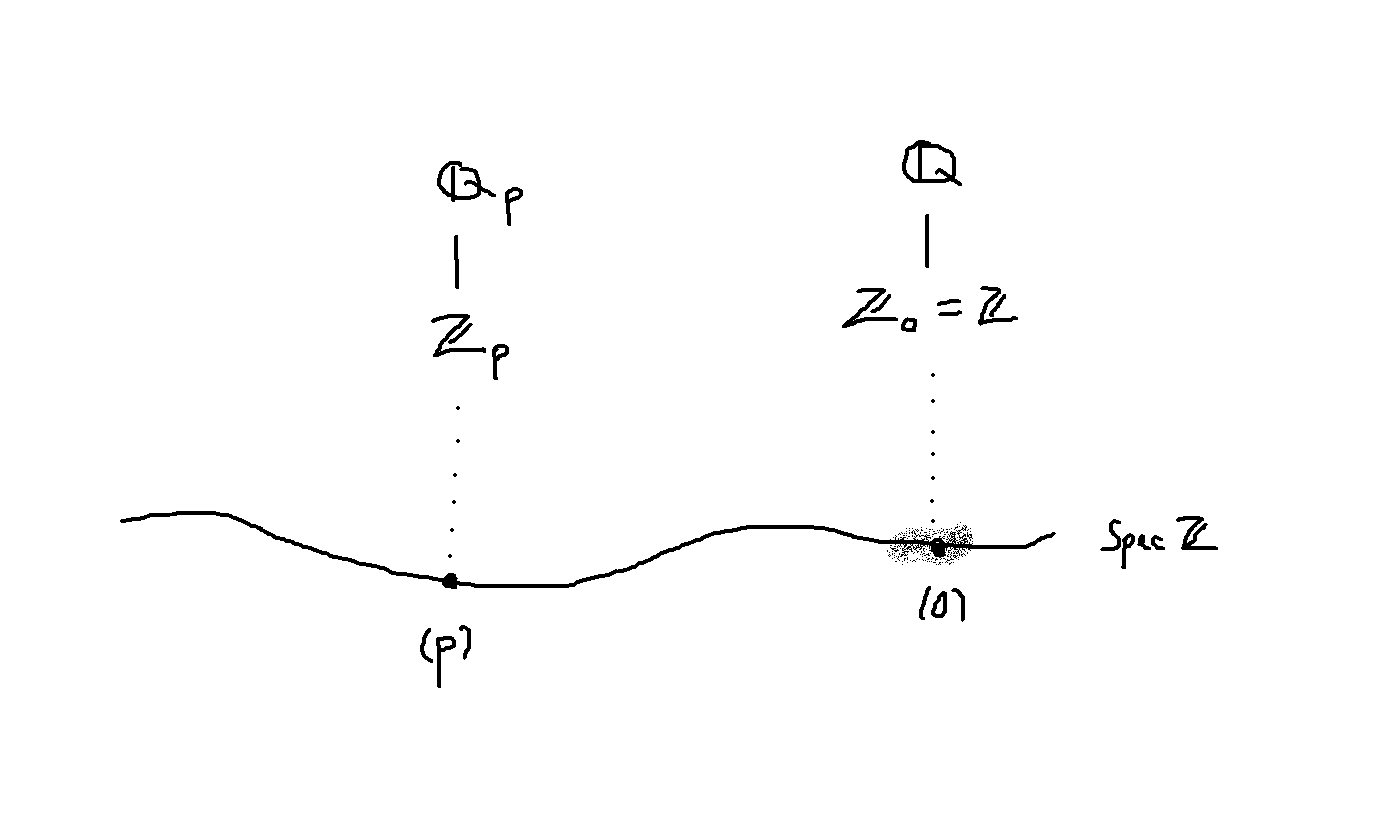
\includegraphics[width=\linewidth,height=\textheight,keepaspectratio]{Figures/places of Spec Z.png}
                        \caption{Places of $\Q$ (note that $(0)$ should be viewed as the generic place-at-infinity).}
                        \label{fig: places_of_Q}
                    \end{figure}
            \end{convention}
            
            \begin{proposition}[Local-global compatibility]
            
            \end{proposition}
                \begin{proof}
                    
                \end{proof}
            
            \begin{example}[Places of ramification of more general arithmetic schemes]
                Below are examples of arithmetic schemes, i.e. schemes over $\Spec \Z$, on which there are primes lying over those of $\Spec \Z$ where ramifications take place.
                    \begin{enumerate}
                        \item \textbf{(The prime spectrum of the ring of integers of a number field):} Consider the following setting:
                            $$
                                \begin{tikzcd}
                                	{\Q(\sqrt{d})} & {\Z[\sqrt{d}]} \\
                                	\Q & \Z
                                	\arrow[no head, from=2-1, to=1-1]
                                	\arrow[no head, from=2-2, to=1-2]
                                	\arrow[no head, from=1-1, to=1-2]
                                	\arrow[no head, from=2-1, to=2-2]
                                \end{tikzcd}
                            $$
                        wherein we are consider the quadratic extension $\Q(\sqrt{d})/\Q$ along with the induced integral extension of Dedekind domains $\Z[\sqrt{d}]/\Z$; particularly, let us pick a prime ideal $\p$ of $\Z$ (i.e. either the zero ideal or an ideal generated by a prime number $p$). Now, do the primes of $\Z[\sqrt{d}]$ indeed lie over those of $\Z$ ? First of all, we will need to see what the prime ideals of $\Z[\sqrt{d}]$ actually look like, and luckily, we can apply corollary \ref{coro: prime_splitting_finite_extensions} to do this:
                            \begin{enumerate}
                                \item Of course, the ideal $(0)\Z[\sqrt{d}]$ is just the zero ideal, and thus admits the trivial factorisation $(0) = (0)$. Because of this, let us only consider non-zero prime ideals of $\Z$ from now on.
                                \item Then, there are three cases, according to corollary \ref{coro: ramification_quadratic_fields}:
                                    \begin{enumerate}
                                        \item 
                                        \item
                                        \item
                                    \end{enumerate}
                            \end{enumerate}
                        \item \textbf{(A conic over $\Spec \Z$):}
                        \item \textbf{(The line with double origin over $\Spec \Z$):}
                    \end{enumerate}
                \end{example}
                
        \subsubsection{Unramfied morphisms}
            \begin{definition}[Unramified morphisms] \label{def: unramified_morphisms}
                A ring map is said to be \textbf{unramified} if it is of finite type and if the corresponding module of K\"ahler differentials is zero. 
            \end{definition}
            \begin{example}
                \noindent
                \begin{itemize}
                    \item \textbf{(\'Etale morphisms):} \'Etale morphisms (cf. definition \ref{def: etale_morphisms}) are trivially unramified. The converse statement is not necessarily true, since there are morphisms of finite type that are not of finite presentation, which is a necessary condition for \'etale-ness (or even just smoothness for that matter).
                    
                    As a concrete example, take any unramified finite extension $E/F$ (cf. definition \ref{def: ramification_indices}), and in the event that these fields have rings of integers (cf. example \ref{example: ring_of_integers}), the induced map:
                        $$\Spec E^{\circ} \to \Spec F^{\circ}$$
                    will also be unramified (in fact, they will be \'etale, since finite extensions come from finite presentations). As a result, for some fixed base scheme $S$, one can think of unramified morphisms $X \to S$ as coming from $S$-schemes $X$ such that preimages of points of $S$ consists merely of a single point. 
                    \item \textbf{(A counter example: non-\'etale smooth morphisms):} A smooth morphism of non-zero relative dimension can not be unramified, since its associated module of K\"ahler differential is not zero. 
                \end{itemize}
            \end{example}
            
            \begin{proposition}[Locality of ramification] \label{prop: locality_of_ramification}
                We say that 
            \end{proposition}
            
        \subsubsection{Extensions of discrete valuation rings}
            
        
        \subsubsection{Galois extensions and ramification}

\section{\'Etale cohomology for schemes: The Chosen One}
    \subsection{\'Etale morphisms} %\label{subsection: etale_morphisms}
        \begin{definition}[\'Etale morphisms] \label{def: etale_morphisms} \index{\'Etale-ness}
            An \'etale ring map is a smooth ring map whose cotangent complex is quasi-isomorphic to the zero complex. Equivalently, a ring homomorphism is \'etale if and only if it is smooth and of relative dimension $0$ (see proposition \ref{prop: smoothness_implies_almost_finiteness_of_cotangent_complex} for an explanation). 
        \end{definition}
        
        \begin{proposition}[The separable extension criterion for \'etale-ness] \label{prop: separable_criterion_for_etaleness} \index{\'Etale-ness! Separability Criterion}
            Let $\pi: F \to B$ be a ring map of finite presentation. Then, the following statements are equivalent:
                \begin{enumerate}
                    \item $\pi$ is \'etale.
                    \item The field extension $\kappa_{\pi^{-1}(\q)}/\kappa_{\q}$ of the residue field at $\pi^{-1}(\q) \in |\Spec k|$ over that at $\q \in |\Spec B|$ is separable (and necessarily finite, as \'etale maps are \textit{a priori} of finite presentation) for all $\q \in |\Spec B|$. Note that the extension $\kappa_{\pi^{-1}(\q)}/\kappa_{\q}$ exists thanks to the fact that the stalk map:
                        $$\calO_{\Spec F, \pi^{-1}(\q)} \to \calO_{\Spec B, \q}$$
                    which is actually just: 
                        $$F_{\pi^{-1}(\q)} \to B_{\q}$$
                    is required to be a local homomorphism between local rings.
                    \item If $F$ is a field, then $B$, when viewed as an $F$-vector space, can be written as a (necessarily finite) direct sum of (necessarily finite) separable extensions of $F$ (of course, this assertion is only equivalent to the other two in the event that they are considered with $F$ a field as well).
                \end{enumerate}
        \end{proposition}
            \begin{proof}
                This is trivial when $\chara \kappa_{\q} = 0$, as every extension in characteristic $0$ is \textit{a priori} separable (for a proof, please consult \cite[\href{https://stacks.math.columbia.edu/tag/030Q}{Tag 030Q}]{stacks} and \cite[\href{https://stacks.math.columbia.edu/tag/030N}{Tag 030N}]{stacks}). Thus, let us assume that:
                    $$\chara \kappa_{\q} = p$$
                for some prime $p$. Also, note that the extension $\kappa_{\pi^{-1}(\q)}/\kappa_{\q}$ decomposes into a separable part $\kappa_{\q}^{\sep}/\kappa_{\q}$ (with $\kappa_{\q}^{\sep}$ is the separable closure of $\kappa_{\q}$ inside $\kappa_{\pi^{-1}(\q)}$) and a purely inseparable part $\kappa_{\pi^{-1}(\q)}/\kappa_{\q}^{\sep}$ in the following manner \cite[\href{https://stacks.math.columbia.edu/tag/030K}{Tag 030K}]{stacks}:
                    $$
                        \begin{tikzcd}
                        	{\kappa_{\pi^{-1}(\q)}} \\
                        	{\kappa_{\q}^{\sep}} \\
                        	{\kappa_{\q}}
                        	\arrow[no head, from=3-1, to=2-1]
                        	\arrow[no head, from=2-1, to=1-1]
                        \end{tikzcd}
                    $$
                \begin{enumerate}
                    \item 
                        \begin{enumerate}
                            \item \textbf{(1 implies 2):} Suppose firstly that \textbf{1} holds, i.e. that $\pi: F \to B$ is \'etale. According to definition \ref{def: etale_morphisms}, this tells us that $B$ is a smooth $F$-algebra that is of relative dimension $0$; in other words, we can write $B$ as $\frac{F[x_1, ..., x_n]}{(f_1, ..., f_n)}$ for some natural number $n$. Now, fix an arbitrary prime ideal $\q \in \left|\Spec \frac{F[x_1, ..., x_n]}{(f_1, ..., f_n)}\right|$, which should be noted to be nothing but a prime of $F[x_1, ..., x_n]$ containing the ideal $(f_1, ..., f_n)$, and note that:
                                $$\left(\frac{F[x_1, ..., x_n]}{(f_1, ..., f_n)}\right)_{\q} \cong \frac{F[x_1, ..., x_n]_{\q}}{(f_1, ..., f_n)}$$
                            thanks to the fact that colimits commute. Now, let us suppose for the sake of deriving a contradiction, that $\kappa_{\pi^{-1}(\q)}/\kappa_{\q}$ is not a (finite) separable extension for our chosen prime $\q$, and observe that according to the preliminary discussion, this is the same as supposing that the purely inseparable extension $\kappa_{\pi^{-1}(\q)}/\kappa_{\q}^{\sep}$ is non-trivial. 
                            \item \textbf{(2 implies 1):} On the other hand, let us use \textbf{2} as our starting point. 
                        \end{enumerate}
                    \item 
                        \begin{enumerate}
                            \item \textbf{(2 implies 3):} Now, suppose that \textbf{2} is true and that $F$ is a field. Immediately, one sees that:
                                $$\kappa_{\pi^{-1}{\q}} \cong \calO_{\Spec F, \pi^{-1}(\q)} \cong F_{\pi^{-1}(\q)} \cong F_{(0)} \cong F$$ 
                            which means that $F/\kappa_{\q}$ is a (finite) separable extension for all primes $\q \in \left|\Spec B\right|$. Also, thanks to the hypothesis whereby $F$ is a field, one can write the finitely presented $F$-algebra $B$ as some finite direct some of copies of $F$ (since algebras are first and foremost modules, and modules over fields are vector spaces, which are \textit{a priori} all free). Thus, the \'etale $F$-algebra $B$, when viewed as a vector space over $F$, can written as a finite direct sum of the finite separable extension $F$ of $\kappa_{\q}$, for all $\q \in |\Spec B|$. In other words, \textbf{2} implies \textbf{3}. 
                            \item \textbf{(3 implies 2):} Conversely, suppose that \textbf{3} is true, specifically that:
                                $$B \cong F^{\oplus d}$$
                            for some natural number $d$, and suppose that the $F$-algebra of finite presentation $B$ is of the form $\frac{F[x_1, ..., x_N]}{(f_1, ..., f_n)}$, for some pair of natural numbers $n, N$. 
                        \end{enumerate}
                    Thus, we have managed to show that \textbf{1} is equivalent to \textbf{2}, and that \textbf{2} is in turn equivalent to \textbf{3}, and thus the three are jointly equivalent. 
                \end{enumerate}
            \end{proof}
        \begin{corollary}[Finite separable extensions are \'etale] \label{coro: finite_separable_extensions_are_etale}
            Let $k$ be a field and let $B$ be a $k$-algebra of finite presentation. According to proposition \ref{prop: separable_criterion_for_etaleness}, $B$ is \'etale over $k$ if and only if when it is viewed as a $k$-vector space, $B$ is a direct sum of copies of some finite separable extension $K$ over $k$. But $K$ itself is a $k$-algebra, and thus every finite and separable field extension is an \'etale ring map. In fact, it is even better: via the adjoint equivalence:
                $$
                    \begin{tikzcd}
                    	{{}^{k/}\Comm\Alg^{\op}} & {\Sch^{\aff}_{/\Spec k}}
                    	\arrow[""{name=0, anchor=center, inner sep=0}, "\Spec"', shift right=2, from=1-1, to=1-2]
                    	\arrow[""{name=1, anchor=center, inner sep=0}, "Gamma"', shift right=2, from=1-2, to=1-1]
                    	\arrow["\dashv"{anchor=center, rotate=-90}, draw=none, from=1, to=0]
                    \end{tikzcd}
                $$
            any non-empty collection of finite separable extension $\{k \to K_{\alpha}\}_{\alpha \in A}$ of some given ground field $k$ corresponds to an \'etale covering sieve $\{\Spec K_{\alpha} \to \Spec k\}_{\alpha}$ (because spectra of fields are singletons, the joint surjection of presheaves:
                $$
                    \begin{tikzcd}
                    	{\left(\coprod_{\alpha \in A} h_{\Spec K_{\alpha}}\right) \x_{h_{\Spec k}} \left(\coprod_{\alpha \in A} h_{\Spec K_{\alpha}}\right)} & {\coprod_{\alpha \in A} h_{\Spec K_{\alpha}}} & {h_{\Spec k}}
                    	\arrow["{\pr_2}"', shift right=2, from=1-1, to=1-2]
                    	\arrow["{\pr_1}", shift left=2, from=1-1, to=1-2]
                    	\arrow[dashed, from=1-2, to=1-3]
                    \end{tikzcd}
                $$
            exists for all non-empty indexing sets $A$). In turn, this implies something remarkable, which is that for all Galois extensions $K/k$ (which are necessarily separable by definition, and hence \'etale) and for all \textit{sheaves} $\calF$ on ${}^{k/}\Comm\Alg^{\op, \petit}_{\et}$ (we refer the reader to paragraph \ref{paragraph: etale_descent} for the descent theory along \'etale morphisms) we have via the fact that finite colimits (in this case, the orbit space ) commute with filtered limits that and the Fundamental Theorem of Galois Theory that:
                $$
                    \begin{aligned}
                        F(\Spec K)/Gal(K/k) & \cong \calF(\Spec E)/\left(\underset{E}{\lim} \Aut(E/k)\right)
                        \\
                        & \cong \underset{E}{\lim} \left(\calF(\Spec E)/\Aut(E/k)\right)
                        \\
                        & \cong \underset{E}{\lim} \left(\calF(\Spec k)/\Aut(E/k)\right)
                    \end{aligned}
                $$
            wherein the limit is the filtered limit taken over the poset of finite separable subextensions $E/k$ of $K/k$; also, note that:
                $$\calF(\Spec E) \cong \calF(\Spec k)$$
            for all finite separable extensions $E/k$ because sheaves satisfy descent, by definition.
        \end{corollary}
        \begin{remark}[Fibres over rational points of \'etale morphisms and inertia of primes] \label{remark: fibres_of_etale_maps_over_points}
            Let $k$ be a field and let $B$ be an \'etale $k$-algebra. From proposition \ref{prop: separable_criterion_for_etaleness}, we know that there exists a natural number $d$ such that:
                $$B \cong K^{\oplus d} \cong (k^{\oplus [K : k]})^{\oplus d} \cong k^{\oplus ([K : k] \cdot d)}$$
            as $k$-vector spaces, where $K/k$ is some finite separable extension. Then, thanks to the fact that direct sums of algebra objects in the category $k\Vect$ of $k$-vector spaces are merely products in the commutative algebra category ${}^{k/}\Comm\Alg$, and by employing the adjoint equivalence:
                $$
                    \begin{tikzcd}
                    	{{}^{k/}\Comm\Alg^{\op}} & {\Sch^{\aff}_{/\Spec k}}
                    	\arrow[""{name=0, anchor=center, inner sep=0}, "\Spec"', shift right=2, from=1-1, to=1-2]
                    	\arrow[""{name=1, anchor=center, inner sep=0}, "Gamma"', shift right=2, from=1-2, to=1-1]
                    	\arrow["\dashv"{anchor=center, rotate=-90}, draw=none, from=1, to=0]
                    \end{tikzcd}
                $$
            one gets:
                $$\Spec B \cong \Spec \prod_{i = 1}^d K \cong \coprod_{i = 1}^d \Spec K$$
            wherein the coproduct is taken in the category of locally ringed spaces over $\Spec k$, but lands in the category of affine schemes (also over $\Spec k$). Lastly, because spectra of fields are singletons, the \'etale $k$-algebra $B$ is nothing but a collection of $d$ disjoint points lying over the single point of $\Spec k$. 
            
            One implication of this is that given any scheme $X$ over $\Spec k$, its fibres over $k$-rational points $x \in X(k)$ are nothing but finite collections of points (even if the fibre is not affine, its affine patches would still necessarily be finite collections of points, as shown above, and thus the whole fibre would be so as well).
        \end{remark}

    \subsection{Galois cohomology}
        \subsubsection{Cohomology of profinite groups}
            Cohomology of profinite groups is nothing but group cohomology but for pro-objects in the category of finite groups (for us, cohomology shall always mean cohomology with abelian coefficients). Because of that, we shall pay less attention to the definition and general properties, and more on the special properties that cohomologies of profinite groups enjoy. By the end of it, we shall apply what we know to Galois groups, which are profinite thanks to the Fundamental Theorem of Galois Theory. 
            
            \paragraph{Group cohomology}
                \begin{convention}
                    \noindent
                    \begin{itemize}
                        \item Throughout, we shall work with a sheaf topos $\E$ in which the category of internal abelian groups $\Ab(\E)$ has enough projectives (for instance, one can consider $\E \cong \Sets$ or the \'etale topos over any qcqs scheme). This essentially just means that we are assuming that the internal logic of $\E$ supports the Axiom of Choice (or more minimally, the Axiom of Presentation). 
                        
                        In particular, fix an abelian group $A \in \Ab(\E)$.
                        \item Additionally, fix a group object $G \in Grp(\E)$. Its group ring shall be denoted by $\Z[G]$ (which is not an abuse of notation, since a natural number object exists in $\E$, allowing us to define an integer object $\Z$ as the group completion of the monoid $\N$; alternatively, one can think of $\Z$ as the monoidal unit of $\Ab(\E)$); recall that this ring object is defined via the following forgetful-free adjunction, whose existence we shall let the reader prove as an exercise\footnote{Recall that $\Ring(\E)$ is the category of monoids internal to the symmetric monoidal category $\Ab(\E)$.}:
                            $$
                                \begin{tikzcd}
                                	{\Ring(\E)} & {\Grp(\E)}
                                	\arrow[""{name=0, anchor=center, inner sep=0}, "\oblv"', shift right=2, from=1-1, to=1-2]
                                	\arrow[""{name=1, anchor=center, inner sep=0}, "{\Z[-]}"', shift right=2, from=1-2, to=1-1]
                                	\arrow["\dashv"{anchor=center, rotate=-90}, draw=none, from=1, to=0]
                                \end{tikzcd}
                            $$
                            
                        We shall also want a $G$-action on $A$, which would make $A$ a $\Z[G]$-module.
                    \end{itemize}
                \end{convention}
                
                \begin{definition}[Group cohomologies] \label{def: group_cohomologies}
                    The $n^{th}$ cohomology group of $G$ with coefficient in $A$ is defined as:
                        $$H^n(G, A) \cong \Ext^n_{\Z[G]}(\Z, A)$$
                    where we view $\Z$ as trivial $G$-representation on the right-hand side. 
                \end{definition}
                \begin{remark}
                    It is not hard to see via induction on the cohomological dimension $n \in \N$ that $H^n(G, A)$ (as in definition \ref{def: group_cohomologies}) actually has a $k$-module structure.
                \end{remark}
                
                Let us now attempt to compute cohomologies of groups in low dimensions (namely, $n = 0, 1, 2$) as well as give meaning to these spaces, which we shall do using free (or at worst, projective) resolutions of the trivial $\Z[G]$-module $\Z$.
                \begin{proposition}[Low-dimensional cohomologies of groups] \label{prop: low_dimensional_cohomologies_of_groups}
                    One has the following interpretations of the low-dimensional cohomologies of $G$ with coeffcients in $A$:
                    \begin{enumerate}
                        \item \textbf{($n = 0$: Invariants):}
                            $$H^0(G, A) \cong A^G$$
                        with $A^G$ denoting the space of $G$-fixed point of $A$.
                        \item \textbf{($n = 1$: Torsors):} 
                        \item \textbf{($n = 2$: Extensions):} 
                            $$H^2(G, A) \cong \{\text{extensions of $G$ by $A$}\}$$
                    \end{enumerate}
                \end{proposition}
                    \begin{proof}
                        \noindent
                        \begin{enumerate}
                            \item \textbf{($n = 0$: Invariants):}
                            \item \textbf{($n = 1$: Torsors):}
                            \item \textbf{($n = 2$: Extensions):}
                        \end{enumerate}
                    \end{proof}
                \begin{example}
                                
                \end{example}
            
            \paragraph{Properties of cohomologies of profinite groups}
        
        \subsubsection{Iwasawa theory}
        
    \subsection{\'Etale fundamental groups}
        \subsubsection{Construction of \'etale fundamental groups}
            \'Etale fundamental groups of schemes as in \cite[Expos\'e V]{SGA1} are constructed using so-called \textbf{finite Galois categories}: in particular, for any fixed scheme $X$, the category of finite \'etale $X$-schemes is an instance of a finite Galois category, for whom the fundamental group is the group of natural automorphisms of the \textbf{fibre functor} based at a geometric point $\bar{x} \in X$:
                $$\Fib_{\bar{x}}: (\Sch_{/X})_{\fet} \to \Fin\Sets$$
                $$Y \mapsto Y(\bar{x})$$
            Below shall be a brief discussion of the construction (remark \ref{remark: finite_etale_schemes}) and key properties of \'etale fundamental groups of schemes (propositions \ref{prop: etale_fundamental_groups_do_not_depend_on_base_points} and \ref{prop: etale_homotopy_exact_sequence}), accompanied by certain relevant examples (cf. examples \ref{example: etale_fundamental_group_of_a_field} and \ref{example: etale_fundamental_group_of_a_curve}). 
            
            We begin with the notion of finite Galois categories. Heuristically speaking, these are categories which are equivalent to $\pi\-\Fin\Sets$, the category of finite sets with actions of some profinite group $\pi$, which as we shall see, serves as the \say{fundamental group} of its associated finite Galois category. Due to this phenomenon, the fundamental group of a Galois category serves the same purpose as the classical fundamental groups of topological spaces, that being as a topological invariant. 
            \begin{definition}[Finite Galois categories] \label{def: finite_galois_categories}
                \noindent
                \begin{itemize}
                    \item \textbf{(Finite Galois categories):} A \textbf{finite Galois category} is defined via the data contained in a pair $(\calG, F)$ consisting of:
                    \begin{itemize}
                        \item a \textit{finitely complete and finitely cocomplete} small category $\calG$, wherein objects can all be written as finite coproducts of \textit{connected} objects\footnote{Objects $Y \in \calG$ such that the copresheaf $h^Y: \calG \to \Sets$ preserves all coproducts.}, and
                        \item a \textit{pro-representable} functor $F: \calG \to \Fin\Sets$, called the \textbf{fibre functor}, which we shall require to be reflect and preserve all finite limits and finite colimits.
                    \end{itemize}
                    \item \textbf{(Galois objects):} An object $Y$ of a finite Galois category $\calG$ is a \textbf{Galois object} if and only if $Y/\Aut(Y)$ is terminal as an object of $\calG$ (which exists as $\calG$ is finitely complete by definition).
                    \item \textbf{(Galois functors):} A \textbf{Galois functor} is an exact functor $\Phi: \calG \to \calG'$ between finite Galois categories $(\calG, F), (\calG', F')$ which preserves connected objects and commute with the fibre functors in the following manner:
                        $$
                            \begin{tikzcd}
                            	\calG && {\calG'} \\
                            	& \Fin\Sets
                            	\arrow["F"', from=1-1, to=2-2]
                            	\arrow["{F'}", from=1-3, to=2-2]
                            	\arrow["\Phi", from=1-1, to=1-3]
                            \end{tikzcd}
                        $$
                \end{itemize}
            \end{definition}
            \begin{remark}
                What we refer to as \say{finite Galois categories} here are simply \say{Galois categories} in both \cite[Expos\'e V]{SGA1} and \cite[\href{https://stacks.math.columbia.edu/tag/0BMQ}{Tag 0BMQ}]{stacks}. We have done this in order to highlight the relationship between our \say{finite Galois categories} and the \say{infinite Galois categories} from \cite[Section 7]{bhatt_scholze_2014_pro_etale} (cf. definition \ref{def: infinite_galois_categories}).
            \end{remark}
            
            \begin{lemma}[Galois covers of connected objects] \label{lemma: galois_covers_of_connected_objects}
                \cite[\href{https://stacks.math.columbia.edu/tag/0BN2}{Tag 0BN2}]{stacks} Let $(\calG, F)$ be a finite Galois category and let $Y$ be a connected object. Then, there exits a Galois object $\tilde{Y}$ and a morphism $\tilde{p}: \tilde{Y} \to Y$.
            \end{lemma} 
            \begin{corollary}[Cofiltered diagrams of Galois objects] \label{coro: cofiltered_diagrams_of_Galois_objects_in_a_finite_Galois_category}
                If $(\calG, F)$ is a finite Galois category then the full subcategory of Galois objects is cofiltered (cf. \cite[\href{https://stacks.math.columbia.edu/tag/00D3}{Tag 00D3}]{stacks}).
            \end{corollary}
            \begin{remark}
                Lemma \ref{lemma: galois_covers_of_connected_objects} ought to be thought of as a vast generalisation of the fact that every separable extension admits a Galois closure (or perhaps more fundamentally, the fact that every subgroup admits a normal closure). Why this is the case can be seen using the Galois Correspondence for fields (or alternatively, the Galois Correspondence for covering spaces; cf. \cite[Theorem 1.38]{hatcher2002algebraic}): if $L/K$ is a Galois extension then subgroups $H \leq \Gal(L/K)$ are normal if and only if the corresponding subextension is normal and likewise, if $Y \to Y' \to X$ is a tower of connected coverings then $\Aut(Y'/X)$ is a normal subgroup of $\Aut(Y/X)$ if and only if $Y' \to X$ is Galois\footnote{We have omitted certain mild technical assumptions here. For a more detailed account, see \cite[Section 1.3]{hatcher2002algebraic}.}. 
            \end{remark}
            \begin{lemma}[Morphisms between connected objects are epic] \label{lemma: morphisms_between_connected_objects_are_epic}
                In any finite Galois category, morphisms between connected objects are epimorphisms and vice versa, the codomain of an epimorphism whose domain is connected is also connected.
            \end{lemma}
                \begin{proof}
                    See \cite[\href{https://stacks.math.columbia.edu/tag/0BN0}{Tag 0BN0}]{stacks} and \cite[Proposition 3.5]{nlab:connected_objects}.
                \end{proof}
            \begin{proposition}[Fibre functors of finite Galois categories are pro-represented by Galois objects] \label{prop: fibre_functors_of_finite_galois_categories_are_pro_represented_by_galois_objects}
                \cite[\href{https://stacks.math.columbia.edu/tag/0BN3}{Tag 0BN3}]{stacks} Let $(\calG, F)$ be a finite Galois category. Then, the fibre functor $F$ is pro-represented by any cofinal diagram in the full subcategory spanned by Galois objects of $\calG$.
            \end{proposition}
            \begin{corollary}[There is only one fibre functor!] \label{coro: only_one_fibre_functor_on_a_finite_galois_category}
                Let $\calG$ be a finite Galois category and let $F, F'$ be fibre functors thereon. Then $F \cong F'$, as they are pro-represented by cofinal pro-object of $\calG$.
            \end{corollary}
            
            \begin{definition}[Fundamental groups of finite Galois categories] \label{def: fundamental_groups_of_finite_galois_categories}
                The \textbf{fundamental group} of a given finite Galois category $(\calG, F)$, denoted by $\pi_1(\calG, F)$, is defined to be $\Aut(F)$.
            \end{definition}
            
            \begin{definition}[Profinite completions of groups] \label{def: profinite_completions_of_groups}
                The \textbf{profinite completion} of a topological group $G$, denoted by $\hat{G}$, is the limit in $\Sets$ of the cofiltered diagram $\{G/N\}_{\text{$N \leq G$ open, normal, finite-index}}$. 
            \end{definition}
            \begin{proposition}[Finite Galois categories of equivariant finite sets] \label{prop: finite_galois_categories_of_equivariant_finite_sets}
                Let $G$ be a topological group and let $\oblv_G: G\-\Fin\Sets \to \Fin\Sets$ denote the forgetful functor going from the category of finite sets with continuous actions of $G$, to that of finite sets. Then there is an isomorphism of profinite groups $\Aut(\oblv_G) \cong \hat{G}$. Furthermore, $G\-\Fin\Sets$ is a finite Galois category if and only if $G$ is a profinite group. 
            \end{proposition}
                \begin{proof}
                    Combine \cite[IV.2.4 et IV.2.7]{sga4} with \cite[\href{https://stacks.math.columbia.edu/tag/0BMU}{Tag 0BMU}]{stacks}.
                \end{proof}
                
            \begin{lemma}[Endomorphisms on Galois objects are automorphisms] \label{lemma: endomorphisms_on_galois_objects_of_finite_galois_categories_are_automorphisms}
                \cite[pp. 100]{SGA1} All endomorphisms on a Galois object of a finite Galois category are automorphisms.
            \end{lemma}
            \begin{proposition}[Fundamental groups of finite Galois categories are profinite] \label{prop: fundamental_groups_of_finite_galois_categories_are_profinite}
                The fundamental group of any finite Galois category is profinite. In fact, given a finite Galois category $(\calG, F)$, its fundamental group arises as the limit of the cofiltered diagram $\{\Aut(F(Y_i))\}_{i \in \calI}$, where $\calI$ is any cofinal diagram of Galois objects in $\calG$.
            \end{proposition}
                \begin{proof}
                    Using proposition \ref{prop: fibre_functors_of_finite_galois_categories_are_pro_represented_by_galois_objects}, suppose that $F \cong \underset{i \in \calI}{\colim} h^{Y_i}$, with $\{Y_i\}_{i \in \calI}$ being a cofinal diagram of Galois objects. From this, and from the fact that all fibre functors on the same finite Galois category are isomorphic (cf. corollary \ref{coro: only_one_fibre_functor_on_a_finite_galois_category}), one sees that:
                        $$\pi_1(\calG, F) \cong \Aut(F) \cong \Nat(F, F) \cong \underset{i \in \calI}{\lim} \Nat(h^{Y_i}, h^{Y_i}) \cong \underset{i \in \calI}{\lim} \calG(Y_i, Y_i)$$
                    Since all endomorphisms on a Galois object of a finite Galois category are automorphisms (cf. lemma \ref{lemma: endomorphisms_on_galois_objects_of_finite_galois_categories_are_automorphisms}), the above tells us that $\pi_1(\calG, F) \cong \underset{i \in \calI}{\lim} \Aut(Y_i)$. Finally, because $F$ reflects isomorphisms by definition, we have an isomorphism $\Aut(Y_i) \cong \Aut(F(Y_i))$ for all $Y_i$; this implies that $\pi_1(\calG, F) \cong \underset{i \in \calI}{\lim} \Aut(F(Y_i))$, which concludes the proof.
                \end{proof}
            \begin{corollary}[Fundamental groups of finite Galois categories act transitively on connected objects] \label{coro: fundamental_groups_of_finite_galois_categories_act_transitively_on_connected_objects}
                Let $(\calG, F)$ be a finite Galois category. Then, $\pi_1(\calG, F)$ acts\footnote{See remark \ref{remark: action_of_fundamental_groups_on_fibres_finite_galois_categories} for an explanation of why such actions even existed in the first place.} transitively and continuously on $F(Y)$ whenever $Y$ is connected. Furthermore, the functor $F$ preserves connectedness of objects. 
            \end{corollary}
            
            \begin{definition}[The compact-open topology] \label{def: the_compact_open_topology}
                Let $X, Y$ be topological spaces and for all $K \subseteq X$ closed (respectively, compact) and all $V \subseteq Y$ open, set $\<K, U\> := \{\varphi \in \Maps(X, Y) \mid \varphi(K) \subseteq U\}$. Then, it can be shown that the collection of sets $\<K, U\>$ as above generates a topology on $\Maps(X, Y)$, which is known as the \textbf{closed-open} (respectively, \textbf{compact-open}) topology.
            \end{definition}
            \begin{lemma}[The compact-open topology on automorphism groups] \label{lemma: the_compact_open_topology_on_automorphism_groups}
                \cite[Theorem 3.5.2 and Corollary 3.5.3]{topological_groups_and_related_structures} Let $X$ be a normal topological space. Then, $\Aut(X)$ will become a topological group if endowed with the subspace topology induced by the closed-open topology on $\Maps(X, X)$. If $X$ is furthermore a compact Hausdorff space then the closed-open and compact-open topologies on $\Aut(X)$ will coincide.
            \end{lemma}
            \begin{example}[The compact-open topology on automorphism groups of sets] \label{example: the_compact_open_topology_on_automorphism_groups_of_sets}
                \noindent
                \begin{itemize}
                    \item \textbf{(Discrete sets):} \cite[\href{https://stacks.math.columbia.edu/tag/0BMC}{Tag 0BMC}]{stacks} If $S$ is a set equipped with the discrete topology, then $\Aut(S)$ shall naturally be a topological group if equipped with either the closed-open topology or the compact-open topology. However, because discrete sets are compact if and only if they are finite, the two topologies can only coincide in that situation.
                    \item \textbf{(Profinite sets):} If $S$ is a profinite set (hence compact and Hausdorff; cf. \cite[\href{https://stacks.math.columbia.edu/tag/08ZY}{Tag 08ZY}]{stacks}) then $\Aut(S)$ shall be the same topological group, regardless of whether it is equipped with the or closed-open topology or the compact-open topology. 
                \end{itemize}
            \end{example}
            \begin{remark}[Action of fundamental groups on fibres] \label{remark: action_of_fundamental_groups_on_fibres_finite_galois_categories}
                Let $(\calG, F)$ be a finite Galois category. First of all, note that because such categories are small and because the category of groups has all (small) products, the product $\prod_{Y \in \Ob(\calG)} \Aut(F(Y))$ is well-defined as a (discrete) group. Now, if we were to endow each $\Aut(F(Y))$ with the subspace topology\footnote{Which is discrete when $F(Y)$ (or rather, $\Aut(F(Y))$) is finite (cf. example \ref{example: the_compact_open_topology_on_automorphism_groups_of_sets}).} inherited from $\Maps(F(X), F(X))$ with the compact-open topology, and then $\pi_1(\calG, F) := \Aut(F)$ with the subspace topology inherited from the product topology on $\prod_{Y \in \Ob(\calG)} \Aut(F(Y))$, then $\pi_1(\calG, F)$ shall act \textit{continuously} on the sets $F(X)$, as seen from the following commutative diagram of topological groups and continuous homomorphisms:
                    $$
                        \begin{tikzcd}
                        	{\pi_1(\calG, F)} & {\prod_{Y \in \Ob(\calG)} \Aut(F(Y))} \\
                        	& {\Aut(F(Y))}
                        	\arrow[tail, from=1-1, to=1-2]
                        	\arrow[two heads, from=1-2, to=2-2]
                        	\arrow[dashed, from=1-1, to=2-2]
                        \end{tikzcd}
                    $$
                As such, the fibre functor $F: \calG \to \Fin\Sets$ factors in the following manner through the category $\pi_1(\calG, F)\-\Fin\Sets$ of finite sets operated on continuously by $\pi_1(\calG, F)$:
                    $$
                        \begin{tikzcd}
                        	\calG && {\pi_1(\calG, F)\-\Fin\Sets} \\
                        	& \Fin\Sets
                        	\arrow[dashed, from=1-1, to=1-3]
                        	\arrow["F"', from=1-1, to=2-2]
                        	\arrow["{\oblv_{\pi_1(\calG, F)}}", from=1-3, to=2-2]
                        \end{tikzcd}
                    $$
                wherein $\oblv_{\pi_1(\calG, F)}: \pi_1(\calG, F)\-\Fin\Sets \to \Fin\Sets$ denotes the forgetful functor. Eventually, we will show that this factorisation is actually a Galois equivalence between $\calG$ and $\pi_1(\calG, F)\-\Fin\Sets$ (see theorem \ref{theorem: finite_categorical_galois_correspondence} below).
            \end{remark}
            \begin{theorem}[The Finite Galois Correspondence] \label{theorem: finite_categorical_galois_correspondence}
                \cite[\href{https://stacks.math.columbia.edu/tag/0BN4}{Tag 0BN4}]{stacks} For any finite Galois category $(\calG, F)$, the functor $F: \calG \to \pi_1(\calG, F)\-\Fin\Sets$ is a Galois equivalence (we equip the latter with the forgetful functor to $\Fin\Sets$).
            \end{theorem}
                \begin{proof}
                    This is essentially the same as the proof of theorem \ref{theorem: infinite_categorical_galois_correspondence}. We shall leave the imposing of the relevant finiteness conditions as in definition \ref{def: finite_galois_categories} up to the reader. 
                \end{proof}
            
            Now, the \'etale fundamental group is literally the fundamental group of a Galois category by construction. Namely, it is the fundamental group of the finite Galois category of pointed schemes that are finite \'etale over a pointed base scheme $(X, \bar{x})$ (cf. remark \ref{remark: finite_etale_schemes}). This, however, is not the only interesting feature that the \'etale fundamental group displays; one of the main reason why Grothendieck's \'etale fundamental group gained attention in the first place is that by taking the \'etale fundamental group of an algebraic variety, one actually obtains the absolute Galois of the global function field of said variety. As such, the \'etale fundamental group is a great tool that we can make use of in order to understand Galois groups; in fact, even the use of finite \'etale morphisms has a very concrete field-theoretic reason (cf. \cite[\href{https://stacks.math.columbia.edu/tag/00U3}{Tag 00U3}]{stacks}).
            
            Let us also note that because any topological space with a generic point is contractible \textit{a priori}, and since most interesting schemes (such as varieties) are integral and hence have generic points\footnote{This is more or less due to the fact that the zero ideal is prime in integral domains. For more details, see \cite[\href{https://stacks.math.columbia.edu/tag/01IS}{Tag 01IS}]{stacks-project}.}, the usual topological fundamental group is very unlikely to be able to distinguish the underlying topological spaces of two different schemes. Furthermore, because schemes are actually determined by their structure sheaves as opposed to their underlying topological spaces (e.g. if $\Nil(R)$ denotes the nilradical of a commutative ring then $\Spec R$ and $\Spec R/\Nil(R)$ will be non-isomorphic schemes whose underlying topological spaces are homeomorphic), we should not expect the topological fundamental group to be able to tell two schemes apart from one another. This is not to mention that in most cases, the underlying topological space of a scheme is not path-connected, so a fundamental group defined as the group of homotopy equivalence class of loops would not have made much sense.
            \begin{remark}[Finite-\'etale schemes] \label{remark: finite_etale_schemes}
                For any given by scheme $X$, the small category $(\Sch_{/X})_{\fet}$ of finite-\'etale $X$-schemes is a category wherein:
                    \begin{itemize}
                        \item all finite limits and all finite colimits exist, and
                        \item all objects can be written as a (possibly empty) finite coproduct of connected objects, which happen to be schemes that are \'etale over $X$.  
                    \end{itemize}
                (for a detailed proof, see \cite[\href{https://stacks.math.columbia.edu/tag/0BN9}{Tag 0BN9}]{stacks}) so should we be able to define a fibre functor $(\Sch_{/X})_{\fet} \to \Fin\Sets$, we will have succeeded in putting a finite Galois category structure on $(\Sch_{/X})_{\fet}$. As a matter of fact, such a well-defined fibre functor has good reasons to exist: it is an easy consequence of \cite[\href{https://stacks.math.columbia.edu/tag/00U3}{Tag 00U3}]{stacks} that for any fixed geometric point $\bar{x} \in X$ (corresponding to an algebraic closure\footnote{Certain sources consider geometric points to correspond to separable closures. For us, however, geometric points are algebraically closed fields $K$ so that $\Spec K$ be a Galois object of $(\Sch_{/\Spec K})_{\fet}$. In practice this choice usually does not matter, since we will mostly work over perfect field, and separable closures of perfect fields are algebraically closed.} $\bar{\kappa}_x$ of the residue field of $x \in X$), one has:
                    $$(\Spec \bar{\kappa}_x)_{\fet} \cong \Fin\Sets$$
                (the forward direct simply involves taking the underlying set, and the inverse functors is given by $I \mapsto \coprod_{i = 1}^{|I|} \Spec \bar{\kappa}_x$) and so for any $k$-scheme $X$, one has the following canonical defined functor:
                    $$(\Sch_{/X})_{\fet} \to (\Sch_{/\Spec \bar{\kappa}_x})$$
                    $$Y \mapsto Y_{\bar{x}}$$
                where $Y_{\bar{x}} \cong Y \x_X \Spec \bar{\kappa}_x$; one can then take the underlying set of $Y_{\bar{x}}$ to get the following trivially left-exact\footnote{... and hence pro-representable (cf. \cite[Proposition 3.1]{grothendieck_fga_2}).} functor:
                    $$\Fib_{\bar{x}}: (\Sch_{/X})_{\fet} \to \Fin\Sets$$
                    $$Y \mapsto |Y_{\bar{x}}|$$
                We should also verify that the sets $|Y_{\bar{x}}|$ are indeed finite. To this end, let us first apply the fact that pullbacks of \'etale morphisms are \'etale to see that if $Y$ is affine over $X$ then $Y_{\bar{x}}$ will have to be the spectrum of an \'etale $\bar{\kappa}_x$-algebra; however, according to \cite[\href{https://stacks.math.columbia.edu/tag/00U3}{Tag 00U3}]{stacks}, this means that $Y_{\bar{x}} \cong \Spec (\bar{\kappa}_x)^{\oplus N}$ for some finite $N$. The locality of \'etale-ness and the finiteness of $Y$ as an $X$-scheme then tells us that in general, $Y_{\bar{x}}$ must be a finite disjoint union of affine schemes of the form $\Spec (\bar{\kappa}_x)^{\oplus N}$, meaning that $Y_{\bar{x}} \cong \Spec (\bar{\kappa}_x)^{\oplus N'}$ for some finite $N'$. The set $|Y_{\bar{x}}|$ is therefore always finite. One also sees that an immediate consequence of this proof is that $\Fib_{\bar{x}}$ necessarily \textit{reflects isomorphisms} and is \textit{right-exact}. 
            \end{remark}
            
            The discussion above allows us to make the following important definition.
            \begin{definition}[\'Etale fundamental groups of schemes] \label{def: etale_fundamental_groups_of_schemes}
                For any scheme $X$ with a fixed geometric point $\bar{x}$, the pair $((\Sch_{/X})_{\fet}, \Fib_{\bar{x}})$ as in remark \ref{remark: finite_etale_schemes} defines a finite Galois category in the sense of definition \ref{def: finite_galois_categories}. Its fundamental group is commonly denoted by $\pi_1(X_{\fet}, \bar{x})$ and called the \textbf{\'etale fundamental group} of $X$ based at $\bar{x}$.
            \end{definition}
            
            We can then apply theorem \ref{theorem: finite_categorical_galois_correspondence} directly to get the following topological characterisation of connected schemes via their \'etale fundamental groups.
            \begin{theorem}[The Geometric Galois Correspondence] \label{theorem: geometric_galois_correspondence}
                For $(X, \bar{x})$ a pointed connected scheme, the functor $\Fib_{\bar{x}}: (\Sch_{/X})_{\fet} \to \Fin\Sets$ as in remark \ref{remark: finite_etale_schemes} above is a Galois equivalence of finite Galois categories. 
            \end{theorem}
            \begin{corollary}
                Should $H$ be a finite-index (hence open, since $\pi_1(X_{\fet}, \bar{x})$ is profinite \textit{a priori}; cf. proposition \ref{prop: fundamental_groups_of_finite_galois_categories_are_profinite}) normal subgroup of $\pi_1(X_{\fet}, \bar{x})$ and $(X^H, \bar{x}^H)$ be the corresponding Galois $X$-scheme with a choice of base point $\bar{x}^H$ lying over $\bar{x}$, then $\pi_1(X^H_{\fet}, \bar{x}^H) \cong H$. In fact, for any connected pointed scheme $(X, \bar{x})$, there is an equivalence of categories:
                    $$\{\text{Finite \'etale $X$-schemes $Y$ with base points $\bar{y}$ lying over $\bar{x}$}\}$$
                    $$\cong$$
                    $$\{\text{Finite-index subgroups of $\pi_1(X_{\fet}, \bar{x})$}\}$$
                which restricts down to:
                    $$\{\text{Finite \'etale Galois $X$-schemes $Y$ with base points $\bar{y}$ lying over $\bar{x}$}\}$$
                    $$\cong$$
                    $$\{\text{Finite-index \textit{normal} subgroups of $\pi_1(X_{\fet}, \bar{x})$}\}$$
            \end{corollary}
            \begin{example}[The \'etale fundamental group of a field] \label{example: etale_fundamental_group_of_a_field}
                As a sanity check, note that if $K$ is a field then finite-\'etale Galois schemes over $\Spec K$ shall be of the form $\Spec L \to \Spec K$, where $L/K$ is a finite Galois extension, and as a consequence, there are the following equivalences of categories\footnote{In fact, these categories are lattices with meets being intersections of fields/subgroups and joins being the constructions of composite fields/subgroups.}, which demonstrate that theorem \ref{theorem: geometric_galois_correspondence} directly generalises the classical Galois Correspondence:
                    $$\{\text{Finite-index normal subgroups of $\pi_1((\Spec K)_{\fet})$}\}$$
                    $$\cong$$
                    $$\{\text{Finite \'etale Galois schemes over $\Spec K$}\}$$
                    $$\cong$$
                    $$\{\text{Finite Galois extensions of $K$}\}^{\op}$$
                    $$\cong$$
                    $$\{\text{Finite-index normal subgroups of $\Gal(\bar{K}/K)$}\}$$
            \end{example}
            \begin{example}[The \'etale fundamental group of a curve] \label{example: etale_fundamental_group_of_a_curve}
                \noindent
                \begin{itemize}
                    \item \textbf{(Projective line):} Let $k$ be a field. If $X$ is a connected non-singular projective curve over $\Spec k$ with function field $K$, then there is a canonical equivalence between the categories of finite Galois extensions of $K$ and finite \'etale Galois $X$-schemes, which are precisely dominant rational maps whose associated function field extensions are Galois thanks to proposition \ref{prop: curves_and_function_fields}. Through this, it is easy to see that:
                        $$\pi_1(X_{\fet}) \cong \Gal(\bar{K}/K)$$
                    For instance, we have:
                        $$\pi_1((\P^1_k)_{\fet}) \cong \Gal(\bar{k}/k)$$
                    (since the function field of $\P^1_k$ is $k(t)$), which tells us that $\P^1_k$ is simply \'etale-connected if and only if $k$ is algebraically closed (since $\Gal(\bar{k}/k)$ is \textit{a fortiori} trivial in that case). 
                    \item \textbf{(Elliptic curves):} Another interesting case that one might wish to consider is that of elliptic curves; for the sake of simplicity, let us work with an elliptic curve $E$ over an algebraically closed field $k$ of characteristic $0$. First of all, because $k$ is algebraically closed, every $k$-rational point $x \in E(k)$ is automatically geometric; therefore, we might as well work with $x = 0$. Now, it can be shown without too much difficulty (cf. \cite[Proposition 5.11]{kundu_etale_fundamental_group_of_elliptic_curves}) that every scheme finite \'etale over an elliptic curve over any field is automatically Galois. Together with the definition of $\pi_1(E_{\fet})$, this implies that for any cofinal diagram $\{Y_i\}_{i \in \calI}$ in $(\Sch_{/E})_{\fet}$, one has:
                        $$\pi_1(E_{\fet}) \cong \underset{i \in \calI}{\lim} \Aut(F_0(Y_i)) \cong \underset{i \in \calI}{\lim} \Aut(|(Y_i)_0|)$$
                    Luckily, there is a canonical choice of such a cofinal diagram, namely $\{E[n]\}_{n \in \N}$ (cf. \cite[Proposition 3.8]{kundu_etale_fundamental_group_of_elliptic_curves}), which are nothing but the fibres over $0 \in E(k)$ (i.e. kernels) of the $n$-torsion maps $[n]: E \to E$ (this is why we chose the base point $x = 0$). It is well-known that $\Aut(|E[n]|) \cong (\Z/n\Z)^{\oplus 2}$, so by taking the limit, one obtains:
                        $$\pi_1(E_{\fet}) \cong \hat{\Z}^{\oplus 2}$$
                    Elliptic curves over (algebraically closed) fields of positive characteristics $p_0$ behave somewhat differently, but it is also difficult to compute their \'etale fundamental groups (provided). If $E$ is supersingular (i.e. if the $p_0$-torsion map $[p_0]: E \to E$ has trivial kernel) then one has the following description of the \'etale fundamental group of $E$ (cf. \cite[Proposition 5.13]{kundu_etale_fundamental_group_of_elliptic_curves}):
                        $$\pi_1(E_{\fet}) \cong \bigoplus_{(p) \in |\Spec \Z| \setminus \{(0), (p_0)\}} \Z_p^{\oplus 2}$$
                    and otherwise, if $E$ is an ordinary elliptic curve, one has the following (cf. \cite[Proposition 5.14]{kundu_etale_fundamental_group_of_elliptic_curves}):
                        $$\pi_1(E_{\fet}) \cong \Z_{p_0} \oplus \bigoplus_{(p) \in |\Spec \Z| \setminus \{(0), (p_0)\}} \Z_p^{\oplus 2}$$
                \end{itemize}
            \end{example}
        
        \subsubsection{Properties of \'etale fundamental groups}
            Now, let us make sure that the \'etale fundamental group $\pi_1(X_{\fet}, \bar{x})$ as defined in definition \ref{def: etale_fundamental_groups_of_schemes} is meaningful as a formal construction. Namely, we would like to know the behaviours of $\pi_1(X_{\fet}, \bar{x})$ when we change the base point and when we base-change (cf. proposition \ref{prop: etale_fundamental_groups_do_not_depend_on_base_points}), as well as whether or not \'etale fibrations induce homotopy exact sequences of fundamental groups (cf. proposition \ref{prop: etale_homotopy_exact_sequence}). 
            \begin{proposition}[\'Etale fundamental group do not depend on base points] \label{prop: etale_fundamental_groups_do_not_depend_on_base_points}
                \cite[\href{https://stacks.math.columbia.edu/tag/0BQA}{Tag 0BQA}]{stacks} Let $f: Y \to X$ be a morphism of connected qcqs\footnote{quasi-compact and quasi-separated} schemes such that the base change functor $X' \mapsto X' \x_X Y$ is an equivalence of Galois categories between $(\Sch_{/X})_{\fet}$ and $(\Sch_{/Y})_{\fet}$. Then, for any choice of geometric points $\bar{x} \in X$ and $\bar{y} \in Y$, one has the following isomorphism of \'etale fundamental groups $\pi_1(X_{\fet}, \bar{x}) \cong \pi_1(Y_{\fet}, \bar{y})$.
            \end{proposition}
            \begin{corollary}[Uniqueness of \'etale fundamental groups] \label{coro: etale_fundamental_group_uniqueness}
                For any connected qcqs scheme $X$ and any pair of possibly distinct geometric points $\bar{x}, \bar{x}' \in X$, one has any isomorphism of \'etale fundamental groups $\pi_1(X_{\fet}, \bar{x}) \cong \pi_1(X_{\fet}, \bar{x}')$, and therefore it makes sense to only speak of \textit{the} fundamental group of $X$, which we shall denote by $\pi_1(X_{\fet})$.
            \end{corollary}
            
            \begin{proposition}[The \'etale homotopy exact sequence] \label{prop: etale_homotopy_exact_sequence}
                \cite[\href{https://stacks.math.columbia.edu/tag/0C0J}{Tag 0C0J}]{stacks} Let $X$ be a connected scheme. If $f: Y \to X$ be a flat proper morphism of finite presentation whose geometric fibres $Y_{\bar{x}}$ are connected and reduced, then for any geometric point $\bar{x} \in X$, there exists a right-exact sequence of groups as follows:
                    $$\pi_1((Y_{\bar{x}})_{\fet}) \to \pi_1(Y_{\fet}) \to \pi_1(X_{\fet}) \to 1$$
            \end{proposition}
    
    \subsection{\texorpdfstring{$\ell$}{}-adic sheaves and Grothendieck's Galois Theory}
        The process of geometrising class field theory begins with the geometrisation of Galois representations, which thanks to a combination of proposition \ref{prop: curves_and_function_fields} and theorem \ref{theorem: geometric_galois_correspondence} are more or less the same as representations of \'etale fundamental groups of schemes. As such, we seek a geometrisation of representations of \'etale fundamental groups and this will be done via establishing a connection between said representations and a certain kind of abelian sheaves - called \textbf{lisse $\bar{\Q}_{\ell}$-adic sheaves} - on \say{the curve of global class field theory} (cf. convention \ref{conv: automorphic_side_conventions}); our efforts shall culminate in theorem \ref{theorem: galois_representations_are_lisse_sheaves}. In addition, we shall be collecting several facts about the algebra of lisse $\bar{\Q}_{\ell}$-adic sheaves for later use. In particular, we want to keep in mind that lisse $\bar{\Q}_{\ell}$-adic sheaves behave well around tensor products as well as pullbacks and pushforwards.  
    
        \subsubsection{Artin-Rees categories and adic sheaves}
            We begin by building our way up to the notion of \textbf{lisse $\bar{\Q}_{\ell}$-adic sheaves}, which are essential for the statement of the main theorem of this section, namely theorem \ref{theorem: galois_representations_are_lisse_sheaves}. For subtle technical reasons, this involves some abstraction in the form of so-called \textbf{Artin-Rees categories}, which are direct generalisations of categories of adically complete modules over Noetherian rings. Our main reference is \cite[Subsection 1.4]{conrad_etale_cohomology} and \cite[Expos\'e V]{sga5}, which was where the constructions below first appeared.
        
            \begin{definition}[Artin-Rees categories] \label{def: artin_rees_categories}
                The \textbf{Artin-Rees category} associated to an abelian category $\calA$ is the full subcategory of $\calA_{\bullet} := \Pro(\calA)$ spanned by cofiltered diagrams $\{M_n\}_{n \in \Z}$; we denote it by $\calA_{\bullet}^{\AR}$. Of particular interest are the so-called \textbf{null systems}, which are objects $\{M_n\}_{n \in \Z} \in \calA_{\bullet}^{\AR}$ such that there exists $\nu \in \N$ so that for all $n \in \Z$ the morphism $M_n \to M_{n + \nu}$ is zero.
            \end{definition}
            
            \begin{proposition}[Artin-Rees categories are linear and abelian] \label{prop: artin_rees_categories_are_linear_and_abelian}
                \cite[Expos\'e V, Propositions 2.2.2 et 2.4.1]{sga5} For any (locally finite) $\Lambda$-linear\footnote{I.e. if hom-sets of $\calA$ are (locally finite) $\Lambda$-modules (e.g. when $\calA \cong \Lambda\mod$).} abelian category $\calA$, the associated Artin-Rees category $\calA_{\bullet}^{\AR}$ is also a (locally finite) $\Lambda$-linear abelian category, with zero objects being the null systems. In fact, the Artin-Rees category $\calA_{\bullet}^{\AR}$ is the localisation\footnote{In the sense of \cite[\href{https://stacks.math.columbia.edu/tag/02MS}{Tag 02MS}]{stacks}.} of $\calA_{\bullet}$ at the thick\footnote{Cf. \cite[\href{https://stacks.math.columbia.edu/tag/02MO}{Tag 02MO}]{stacks}.} subcategory of null systems, meaning that an isomorphism in $\calA_{\bullet}^{\AR}$ (henceforth referred to as an \textbf{AR-isomorphism}) is a morphism in $\calA_{\bullet}$ whose kernel and cokernel are null. 
            \end{proposition}
            
            \begin{convention}[The setting for adic sheaves] \label{conv: l_adic_sheaves_conventions}
                For our purposes, $\calX$ shall be a scheme that is locally of finite type\footnote{Althought $\calX$ might actually be an algebraic stack of finite type over $S$; for details, see \cite{laszlo_olsson_adic_sheaves_on_artin_stacks_1} and \cite{laszlo_olsson_adic_sheaves_on_artin_stacks_2}. It should also be noted that in \cite[Subsection 1.4]{conrad_etale_cohomology}, it was only required that $\calX$ would be Noetherian, which is not sufficient for us, as $\Bun_{\GL_1}(X)$ is merely locally of finite type, and hence only locally Noetherian \textit{a priori}.} over a base scheme $S$ that is affine, regular, Noetherian\footnote{Note that this implies that $\calX$ is locally Noetherian (cf. \cite[\href{https://stacks.math.columbia.edu/tag/01T6}{Tag 01T6}]{stacks}).} and of dimension $\leq 1$, and of characteristic $p \geq 0$; moreoever, we would like to work under the assumption that every finite-type $S$-scheme $T$ is also of finite cohomological dimension. In addition, $\Lambda$ shall be a discrete valuation ring of mixed characteristic $(0, \ell)$ (for some auxiliary prime $\ell \not = p$) with maximal ideal $\m$, and fraction field $E$.
            \end{convention}
            
            \begin{definition}[Torsion objects in tensor categories] \label{def: torsion_objects_in_tensor_categories}
                Let $A$ be a commutative ring, $I$ be an ideal of $A$, and $\calA$ be an $A$-linear category. Then, the subcategory of $\calA$ spanned by $I$-torsion objects is the one wherein the hom-sets are $\Hom_{\calA/I}(M, N) \cong \Hom_\calA(M, N) \tensor_A A/I$.
            \end{definition}
            \begin{definition}[Adic objects and lisse objects of Artin-Rees categories] \label{def: adic_objects_and_lisse_objects_of_artin_rees_categories}
                Consider the Artin-Rees category $\calA_{\bullet}^{\AR}$ associated to a locally finite $\Lambda$-linear abelian category $\calA$. 
                    \begin{enumerate}
                        \item \textbf{(Adic objects):} $\calA_{\bullet}^{\AR}$ admits a full subcategory, denoted by $\calA_{\bullet}^{\ad}$, whose objects $\{M_n\}_{n \in \Z}$ are such that:
                            \begin{itemize}
                                \item $M_n \cong 0$ for all $n < 0$,
                                \item $M_n$ is $\m^{n + 1}$-torsion for all $n \geq 0$, and
                                \item the canonical maps $\Lambda/\m^{n + 2} \tensor_{\Lambda} \Hom_{\calA_{\bullet}^{\AR}}(M_{\bullet}, N_{\bullet}) \to \Hom_{\calA_{\bullet}^{\AR}}(M_{\bullet}, N_{\bullet})/\m^n$ are isomorphisms of $\Lambda/\m^{n + 1}$-modules for all $n \geq 0$.
                            \end{itemize}
                        Objects of this full subcategory are said to be \textbf{$\m$-adic}.
                        \item \textbf{(Lisse objects):} Let $\calA_{\bullet}^{\fin}$ denote the category of Artin-Rees projective systems of objects of $\calA$ which are simultaneously Artinian and Noetherian. Objects of the category\footnote{Here, the intersection is understood to be at both the level of objects and that of morphisms.} $\calA_{\bullet}^{\lisse} := \calA_{\bullet}^{\ad} \cap \calA_{\bullet}^{\fin}$ are then said to be \textbf{lisse}. 
                    \end{enumerate}
            \end{definition}
            \begin{proposition}[Adic categories are linear and abelian] \label{prop: adic_categories_are_linear_and_abelian}
                Let $\calA$ be a locally finite $\Lambda$-linear abelian category. Then, we shall have a tower $\calA_{\bullet}^{\lisse} \subset \calA_{\bullet}^{\ad} \subset \calA_{\bullet}^{\AR}$ of locally finite $\Lambda$-linear abelian categories, wherein the inclusions are fully faithful exact functors.
            \end{proposition}
            \begin{example}[Adic and lisse $\Lambda$-sheaves] \label{example: adic_sheaves}
                Recall first of all that the category of constructible \'etale sheaves of $\Lambda$-modules on a Noetherian scheme - of which the category $\Lambda\mod^{\cons}(\calX_{\et})$ of constructible sheaves of $\Lambda$-modules on $\calX_{\et}$ is a special case - is a locally finite $\Lambda$-linear closed monoidal category (to see why, combine \cite[Propositions 3.20 and 3.22]{behrend_l_adic_sheaves_for_algebraic_stacks}). Then, the category of adic constructible $\m$-adic sheaves on $\calX$ (also called constructible $\Lambda$-sheaves), commonly denoted by $\Shv_{\Lambda}^{\ad}(\calX)$, is nothing but $\Lambda\mod^{\cons}(\calX_{\et})_{\bullet}^{\ad}$, and the category of lisse $\m$-adic sheaves on $\calX$, denoted by $\Shv_{\Lambda}^{\lisse}(\calX)$ is simply $\Lambda\mod^{\cons}(\calX_{\et})_{\bullet}^{\lisse}$.
            \end{example}
            
            \begin{definition}[$E$-objects] \label{def: E_objects}
                Let $\calA$ be a locally finite $\Lambda$-linear abelian category. Then, we can define the associated category of \textbf{$E$-objects} to be the localisation $\calA \tensor_{\Lambda} E$ at $E$-linear morphisms, i.e. we define:
                    $$\Hom_{\calA \tensor_{\Lambda} E}(M, N) \cong \Hom_{\calA}(M, N) \tensor_{\Lambda} E$$
                It can be easily verified that $\calA \tensor_{\Lambda} E$ is locally finite $E$-linear and abelian.
            \end{definition}
            \begin{definition}[$\bar{E}$-objects] \label{def: bar_E_objects}
                Let $\calA$ be a locally finite $\Lambda$-linear abelian category. We define the associated category $\calA \tensor_{\Lambda} \bar{E}$ of \textbf{$\bar{E}$-objects} via:
                    $$\Hom_{\calA \tensor_{\Lambda} \bar{E}}(M, N) \cong \underset{\text{$E'/E$ finite extensions}}{\colim} \Hom_{\calA}(M, N) \tensor_{\Lambda} E'$$
                Using the fact that associated categories of $E$-objects are abelian and $E$-linear, one can show that associated categories of $\bar{E}$-objects are abelian and $\bar{E}$-linear\footnote{The one technicality to keep in mind is that for finite-dimensional vector spaces, filtered colimits commute with kernels.}. 
            \end{definition}
            \begin{example}[Adic and lisse $E$-sheaves and $\bar{E}$-sheaves] \label{example: E_sheaves}
                Because $\Shv_{\Lambda}^{\ad}(\calX)$ and $\Shv_{\Lambda}^{\lisse}(\calX)$ are locally finite $\Lambda$-linear and abelian (cf. proposition \ref{prop: adic_categories_are_linear_and_abelian}), one can define the categories of constructible adic $E$-sheaves and that of lisse $E$-sheaves on $\calX$ to be $\Shv_E^{\ad}(\calX) \cong \Shv_{\Lambda}^{\ad}(\calX) \tensor_{\Lambda} E$ and $\Shv_E^{\lisse}(\calX) \cong \Shv_{\Lambda}^{\lisse}(\calX) \tensor_{\Lambda} E$. Adic and lisse $\bar{E}$-sheaves can thus also be defined.
            \end{example}
            
        \subsubsection{Operations with adic sheaves}
            The following results shall be used throughout the rest of the paper without any explicit mention (that is, with the notable exception of theorem \ref{theorem: galois_representations_are_lisse_sheaves}). For details, we refer the reader to \cite[Sections 6-8]{laszlo_olsson_adic_sheaves_on_artin_stacks_2} (which is a sequel to \cite{laszlo_olsson_adic_sheaves_on_artin_stacks_1}) and \cite[Sections II.7-II.10]{kiehl_weissauer_weil_conjecture_perverse_sheaves_and_l_adic_fourier_transform}.
            
            \begin{proposition}[Tensor products of constructible adic objects] \label{prop: tensor_products_of_constructible_adic_objects}
                \noindent
                \begin{enumerate}
                    \item \cite[Proposition 6.1]{laszlo_olsson_adic_sheaves_on_artin_stacks_2} For any locally finite $\Lambda$-linear closed monoidal abelian category $(\calA, \tensor, \1)$, the associated categories $\calA_{\bullet}^{\ad}$ and $\calA_{\bullet}^{\lisse}$ of adic and lisse systems are monoidal with respect to term-wise tensor products $M_{\bullet} \tensor N_{\bullet} \cong \{M_n \tensor N_n\}_{n \in \Z}$. In fact, they both embed via fully faithful monoidal exact $\Lambda$-linear functors into $\calA_{\bullet}^{\AR}$, which is also monoidal with respect to term-wise tensor products. 
                    \item \cite[Theorem III.12.2 and Appendix A]{kiehl_weissauer_weil_conjecture_perverse_sheaves_and_l_adic_fourier_transform} Furthermore, $\calA_{\bullet}^{\ad}$ and $\calA_{\bullet}^{\lisse}$ (respectively, $\calA_{\bullet}^{\ad} \tensor_{\Lambda} \bar{E}$ and $\calA_{\bullet}^{\lisse} \tensor_{\Lambda} \bar{E}$ for any choice of algebraic closure $\bar{E}/E$) are closed monoidal categories with respect to these tensor products.
                \end{enumerate}
            \end{proposition}
            \begin{example}[Tensor products of constructible adic sheaves] \label{def: tensor_products_of_constructible_adic_sheaves}
                $\Lambda\mod^{\cons}(\calX_{\et})$ is a locally finite closed monoidal category with respect to tensor products over the constant sheaf $\underline{\Lambda}$ (cf. \cite[\href{https://stacks.math.columbia.edu/tag/093P}{Tag 093P}]{stacks}), so by proposition \ref{prop: tensor_products_of_constructible_adic_objects}, the category $\Shv_{\bar{\Q}_{\ell}}^{\lisse}(\calX)$ of lisse $\bar{\Q}_{\ell}$ sheaves on $\calX$ shall be closed monoidal with respect to the constant sheaf $\underline{\bar{\Q}_{\ell}}$.
            \end{example}
            
            \begin{proposition}[$*$-pullbacks and $*$-pushforwards] \label{prop: *_pullbacks_and_pushforwards_of_l_adic_sheaves}
                For $f: \calX \to \calY$ a morphism of finite type between $S$-schemes that are locally of finite type (with $S$ as in convention \ref{conv: l_adic_sheaves_conventions}), there is an adjoint equivalence whose components $f^*$ and $f_*$ are computed term-wise as in \cite[\href{https://stacks.math.columbia.edu/tag/03PZ}{Tag 03PZ}]{stacks} and  \cite[\href{https://stacks.math.columbia.edu/tag/03PV}{Tag 03PV}]{stacks} respectively:
                    $$
                        \begin{tikzcd}
                        	{\Shv_{\bar{\Q}_{\ell}}^{\lisse}(\calX)} & {\Shv_{\bar{\Q}_{\ell}}^{\lisse}(\calY)}
                        	\arrow[""{name=0, anchor=center, inner sep=0}, "{f_*}"', bend right, from=1-1, to=1-2]
                        	\arrow[""{name=1, anchor=center, inner sep=0}, "{f^*}"', bend right, from=1-2, to=1-1]
                        	\arrow["\dashv"{anchor=center, rotate=-90}, draw=none, from=1, to=0]
                        \end{tikzcd}
                    $$
                Furthermore, the funcotrs $f^*$ and $f_*$ both commute with (external) tensor products of lisse $\bar{\Q}_{\ell}$-sheaves.
            \end{proposition}
                \begin{proof}
                    Combine \cite[Proposition 8.3]{laszlo_olsson_adic_sheaves_on_artin_stacks_2} with \cite[Theorem II.7.1]{kiehl_weissauer_weil_conjecture_perverse_sheaves_and_l_adic_fourier_transform}
                \end{proof}
            
            \begin{definition}[Stalks of constructible adic sheaves] \label{def: stalks_of_constructible_adic_sheaves}
                \cite[Definition 1.4.4.3]{conrad_etale_cohomology} Let $\bar{x} \in \calX$ be a geometric point and $\calF_{\bullet} \in \Shv_{\bar{\Q}_{\ell}}^{\ad}(\calX)$ be a constructible $\bar{\Q}_{\ell}$-sheaf on $\calX$. Then, the \textbf{stalk} at $\bar{x}$ shall be given by $\underset{n \in \N}{\lim} (\calF_n)_{\bar{x}}$, with each term $(\calF_n)_{\bar{x}}$ being computed as stalks of \'etale sheaves (cf. \cite[\href{https://stacks.math.columbia.edu/tag/040R}{Tag 040R}]{stacks}).
            \end{definition}
            \begin{remark}
                As tensor products and $*$-pullbacks/pushforwards of lisse $\bar{\Q}_{\ell}$ are computed term-wise, taking stalks of lisse $\bar{\Q}_{\ell}$-sheaves commutes with those operations.
            \end{remark}
            
            \begin{convention}[Continuous linear representations] \label{conv: continuous_linear_representations}
                From now on, if $G$ is a topological group and $E$ is a topological field then we will be writing $\Rep_E(G)$ for the category of \textit{continuous} $E$-linear representations of $G$. In fact, all representations shall be implicitly assumed to be continuous. Also, for all $n \geq 1$, $\Rep_E^n(G)$ shall be used to denote the subcategory of $n$-dimensional $E$-linear representations of $G$.
            \end{convention}
            \begin{theorem}[Galois representations are lisse $\bar{\Q}_{\ell}$-sheaves] \label{theorem: galois_representations_are_lisse_sheaves}
                \cite[Theorem 1.4.5.7]{conrad_etale_cohomology} Let $\calX$ be a connected Noetherian scheme and fix a geometric point $\bar{x} \in \calX$. Then, there exists a monoidal equivalence given by $\calF \mapsto \calF_{\bar{x}}$, from the symmetric monoidal category $\Shv_{\bar{\Q}_{\ell}}^{\lisse}(\calX)$ of lisse $\bar{\Q}_{\ell}$-sheaves to the symmetric monoidal category $\Rep_{\bar{\Q}_{\ell}}^{\fin}(\pi_1(\calX_{\fet}))$ of finite-dimensional continuous $\bar{\Q}_{\ell}$-linear representations of $\pi_1(X_{\fet})$.
            \end{theorem}

    \subsection{\texorpdfstring{$\ell$}{}-adic cohomology}
        \subsubsection{\texorpdfstring{$\ell$}{}-adic cohomology for schemes: "This is where the fun begins!"}
            Let $X$ be a smooth projective scheme over a base field that is possibly of some prime characteristic $p$. Let $\ell$ be a prime different from $p$. By \say{$\ell$-adic cohomology}, we shall mean the cohomology theory whose cohomology groups are given by:
                $$H^i_{\Q_{\ell}}(X) \cong \underset{n \in \N}{\lim} H_{\et}^i(X, \Z/\ell^{n + 1}\Z) \tensor_{\Z_{\ell}} \Q_{\ell}$$
            This means, among other things, that $\ell$-adic cohomology is effectively a \say{singular cohomology theory} for (smooth projective) schemes. This, however, is not the only amazing property that $\ell$-adic cohomology enjoys: it is also a Weil cohomology theory (see definition \ref{def: weil_cohomology_theories} for a description of what this means). At surface level, this might seem odd, since only \'etale cohomology with torsion coefficients gives satisfactory results. However, this is precisely why we take the limit over the torsion rings $\Z/\ell^{n + 1}\Z$ and then base change to $\Q_{\ell}$: $\Q_{\ell}$ is a field of characteristic $0$, and hence can serve as the field of a coefficients of a Weil cohomology theory (cf. definition \ref{def: weil_cohomology_theories}). 
            
            To check that $\ell$-adic cohomology is indeed a Weil cohomology theory, let us \say{simply} go through the axioms laid out in definition \ref{def: weil_cohomology_theories}. Before we can do that, however, we will first need to actually set up the theory of \'etale $\ell$-adic cohomology.
            
            Now, we are finally ready to verify that \'etale $\ell$-adic cohomology is a Weil cohomology theory.
            \paragraph{Finiteness}
        
            \paragraph{The K\"unneth Formula}
            
            \paragraph{Poincar\'e Duality}
        
            \paragraph{The Lefschetz Conditions}
    
        \subsubsection{The Artin comparison theorem: an \'etale GAGA theorem}
        
        \subsubsection{\texorpdfstring{$\ell$}{}-adic cohomology for algebraic stacks: "Another happy landing!"}
            \paragraph{Finiteness}
        
            \paragraph{The K\"unneth Formula}
            
            \paragraph{Poincar\'e Duality}
        
            \paragraph{The Lefschetz Conditions}
            
\section{Pro-\'etale cohomology for schemes: "Another fine cohomology theory to add to my collection"}
    Despite its successes - particularly its involvement in the proofs of the Weil Conjectures - \'etale cohomology has its shortcomings. For one, \'etale cohomology modules are not actually computed over \'etale sites, but rather, as scalar extensions (to $\overline{\Q_{\ell}}$ in the case of $\ell$-adic cohomology for instance) of the actually \'etale cohomology modules over \'etale sites. Pro-\'etale cohomology theories exist so that such issues could be rectified. 
    
    \begin{remark}[What is the pro-\'etale topology ?]
        For now, we refer the reader to \cite[Definition 4.1.1 and Remark 4.1.3]{bhatt_scholze_2014_pro_etale}.
    \end{remark}
    
    \subsection{The pro-\'etale topology for schemes}
    
    \subsection{Infinite Galois categories and pro-\'etale fundamental groups}
        \subsubsection{The abstract framework}
            \begin{definition}[Infinite Galois categories] \label{def: infinite_galois_categories}
                \noindent
                \begin{itemize}
                    \item \textbf{(Infinite Galois categories):} An \textbf{infinite Galois category} is defined via the data contained in a pair $(\calG, F)$ consisting of:
                    \begin{itemize}
                        \item a \textit{cocomplete and \textit{finitely} complete} small category $\calG$, wherein objects can all be written as a coproduct of connected objects, and
                        \item a functor $F: \calG \to \Sets$, called the \textbf{fibre functor}, which we shall require to reflect and preserve all colimits and all finite limits\footnote{In \cite[Definition 7.2.1]{bhatt_scholze_2014_pro_etale}, it is furthermore required that the fibre functor would be faithful. However, because any functor that preserves and reflect monomorphisms must also be faithful, we need not make this requirement.}.
                    \end{itemize}
                    \item \textbf{(Galois objects):} An object $Y$ of an infinite Galois category $\calG$ is a \textbf{Galois object} if and only if $Y/\Aut(Y)$ is terminal as an object of $\calG$ (which exists as $\calG$ is finitely complete by definition).
                    \item \textbf{(Galois functors):} A \textbf{Galois functor} is a functor $\Phi: \calG \to \calG'$ between infinite Galois categories $(\calG, F), (\calG', F')$ which preserves connected objects, colimits, finite limits, and commute with the fibre functors in the following manner:
                        $$
                            \begin{tikzcd}
                            	\calG && {\calG'} \\
                            	& \Sets
                            	\arrow["F"', from=1-1, to=2-2]
                            	\arrow["{F'}", from=1-3, to=2-2]
                            	\arrow["\Phi", from=1-1, to=1-3]
                            \end{tikzcd}
                        $$
                \end{itemize}
            \end{definition}    
            \begin{definition}[Fundamental groups of infinite Galois categories] \label{def: fundamental_groups_of_infinite_galois_categories}
                The \textbf{fundamental group} of a given infinite Galois category $(\calG, F)$, denoted by $\pi_1(\calG, F)$, is defined to be the automorphism group $\Aut(F)$\footnote{Compare this to definition \ref{def: fundamental_groups_of_finite_galois_categories} and note the lack of profinite completion the current situation.}.
            \end{definition}
            Arbitrary infinite Galois categories turn out to be rather pathological, so we shall introduce a more refined notion, namely that of infinite Galois categories which are \textbf{tame}.  
            \begin{definition}[Tame infinite Galois categories] \label{def: tame_infinite_galois_categories}
                \footnote{Note that this is slightly different from \cite[Definition 7.2.4]{bhatt_scholze_2014_pro_etale}, in that we require furthermore that the fibre functor preserves connectedness instead of merely that $\pi_1(\calG, F)$ acts transitively on $F(X)$ whenever $X$ is connected.} One says that an infinite Galois category $(\calG, F)$ is \textbf{tame}\footnote{The terminology comes from the fact given any Galois extension $L/K$, the corresponding Galois group $\Gal(L/K)$ acts transitively on $L$ (cf. \cite[Proposition I.9.1]{neukirch_2010_algebraic_number_theory}).} whenever the fibre functor $F: \calG \to \Sets$ preserves connectedness\footnote{Compare this to corollary \ref{coro: fundamental_groups_of_finite_galois_categories_act_transitively_on_connected_objects}.} and $\pi_1(\calG, F)$ acts transitively on $F(X)$ for all $X$ connected.
            \end{definition}
            
            Let us now introduce the notion of Noohi groups, which shall serve in this new theory of infinite Galois categories as replacements for the more restrictive notion of profinite groups. The idea is that, similar to how fundamental groups of finite Galois categories, the fundamental group of a \textit{tame} infinite Galois category is Noohi. We shall also see that the notion of Noohi groups subsumes the notion of profinite groups and as such, so too does the notion of tame infinite Galois categories subsume that of finite Galois categories.
            \begin{definition}[Noohi groups] \label{def: noohi_groups}
                \cite[Defintion 7.1.1]{bhatt_scholze_2014_pro_etale} A \textbf{Noohi group} is a Hausdorff topological group $G$ such that $G \cong \Aut(\oblv_G)$ \textit{as topological groups} (here, $\Aut(\oblv_G)$ carries the compact-open topology), with $\oblv_G: G\-\Sets \to \Sets$ being the forgetful functor from the category of sets with continuous $G$-actions into the category of sets. In addition, an (in)finite Galois category that is Galois-equivalent to $G\-\Sets$ for some Noohi group $G$ shall be called a \textbf{Noohi category}.
            \end{definition}
            \begin{remark}[Completions of topological groups] \label{remark: completions_of_topological_groups}
                If $X$ is a topological space then we shall denote its Cauchy completion by $X^+$ (i.e. $X^+$ is the minimal topological space containing $X$, in which all Cauchy filters converge). 
                    \begin{itemize}
                        \item By \cite[Theorem 3.6.10]{topological_groups_and_related_structures}, we know that such a completion exists and is unique for all topological groups; furthermore, every topological group is continuously isomorphic to a dense subgroup of its Cauchy completion. 
                        \item \cite[Theorem 3.6.22]{topological_groups_and_related_structures} Any small product of complete topological groups is also a complete topological group.
                        \item Any closed subgroup of a complete topological group is complete.
                    \end{itemize}
            \end{remark}
            \begin{proposition}[Noohi groups are complete] \label{prop: noohi_groups_are_complete}
                \cite[Proposition 7.1.5]{bhatt_scholze_2014_pro_etale} Let $G$ be a Hausdorff topological group with a basis generated by open subsets. Then, there is an homeomorphic group isomorphism $\psi: \Aut(\oblv_G) \to G^+$. In fact, a Hausdorff topological group is a Noohi group if and only if it is complete and has a basis generated by open subgroups.
            \end{proposition}
            \begin{lemma}[Fundamental groups of infinite Galois categories are Noohi] \label{lemma: fundamental_groups_of_infinite_galois_categories_are_noohi}
                A topological group is Noohi if and only if it is the fundamental group of an infinite Galois category.
            \end{lemma}
                \begin{proof}
                    If $G$ is a Noohi group then by definition $\Aut(\oblv_G) \cong G$. Thus, it shall suffice to demonstrate that the pair $(G\-\Sets, \oblv_G)$ is an infinite Galois category; this is routine (cf. \cite[Section 3]{nlab:category_of_G_sets}), so we shall leave it up to our readers as an exercise.
                
                    Conversely, if $(\calG, F)$ is an infinite Galois category then it shall suffice to show that $\pi_1(\calG, F)$ will be a closed subgroup of $\prod_{Y \in \Ob(\calG)} \Aut(F(Y))$ (which is a well-defined group since it is a small product of groups), as we can demonstrated this product group to be Noohi. For this, we use the fact that $\Aut(S)$ for any set $S$ is complete in the compact-open topology (cf. \cite[Lemma 7.1.4]{bhatt_scholze_2014_pro_etale}), and that $\Aut(S)$ admits a basis generated by open subgroups (cf. \cite[\href{https://stacks.math.columbia.edu/tag/0BMC}{Tag 0BMC}]{stacks}): by combining this with the fact that products of complete groups are complete (cf. remark \ref{remark: completions_of_topological_groups}), one infers that $\prod_{Y \in \Ob(\calG)} \Aut(F(Y))$ endowed with the product topology is complete and admits a basis generated by open subgroups, meaning that it is Noohi (cf. proposition \ref{prop: noohi_groups_are_complete}). Then, to show that $\pi_1(\calG, F)$ is a closed subgroup of $\prod_{Y \in \Ob(\calG)} \Aut(F(Y))$, we shall show that it is complete (see remark \ref{remark: completions_of_topological_groups}). For this, see \cite[\href{https://stacks.math.columbia.edu/tag/0BMR}{Tag 0BMR}]{stacks}.
                \end{proof}
            \begin{corollary}[Noohi categories are tame] \label{coro: noohi_categories_are_tame}
                Noohi categories, as in definition \ref{def: noohi_groups}, are tame infinite Galois categories. 
            \end{corollary}
                
            \begin{remark}[Action of fundamental groups on fibres] \label{remark: action_of_fundamental_groups_on_fibres_infinite_galois_categories}
                By arguing as in remark \ref{remark: action_of_fundamental_groups_on_fibres_finite_galois_categories}, one sees that the fibre functor $F: \calG \to \Sets$ of any infinite Galois category $(\calG, F)$ must factor through $\pi_1(\calG, F)\-\Sets$ in the following manner:
                    $$
                        \begin{tikzcd}
                        	\calG && {\pi_1(\calG, F)\-\Sets} \\
                        	& \Sets
                        	\arrow[dashed, from=1-1, to=1-3]
                        	\arrow["F"', from=1-1, to=2-2]
                        	\arrow["{\oblv_{\pi_1(\calG, F)}}", from=1-3, to=2-2]
                        \end{tikzcd}
                    $$
                As a consequence, functions $F(X) \to F(Y)$ coming from morphisms $X \to Y$ in $\calG$ are automatically $\pi_1(\calG, F)$-equivariant. 
            \end{remark}
            \begin{theorem}[The Infinite Galois Correspondence] \label{theorem: infinite_categorical_galois_correspondence}
                \cite[Theorem 7.2.5(3)]{bhatt_scholze_2014_pro_etale} Any tame infinite Galois categories $(\calG, F)$, the functor $F: \calG \to \pi_1(\calG, F)\-\Sets$ is a Galois equivalence\footnote{As such, every tame infinite Galois category is Noohi.} (we equip $\pi_1(\calG, F)\-\Sets$ with the forgetful functor to $\Sets$ to make it a Noohi category; cf. corollary \ref{coro: noohi_categories_are_tame}).
            \end{theorem}
                \begin{proof}
                    Because $F$ reflects monomorphisms (or more generally, all finite limits, as it is an isomorphism-reflecting left-exact functor; cf. definition \ref{def: infinite_galois_categories}) and because any function $f: S \to T$ can be viewed as a unique monomorphism $\Gamma_f: S \to S \x T$ such that $\pr_1 \circ \Gamma_f = \id_S$, any morphism $p: X \to Y$ in $\calG$ can be viewed as a unique monomorphism $\Gamma_p: X \to X \x Y$ such that $\pr_1 \circ \Gamma_p = \id_X$, which comes from. By combining this with the fact that $F$ commutes with finite limits, and that functions $F(X) \to F(Y)$ coming from morphisms $X \to Y$ in $\calG$ are automatically $\pi_1(\calG, F)$-equivariant (cf. remark \ref{remark: action_of_fundamental_groups_on_fibres_infinite_galois_categories}), we obtain the following bijections, which proves that $F: \calG \to \pi_1(\calG, F)\-\Sets$ is fully faithful:
                        $$
                            \begin{aligned}
                                \calG(X, Y) & \cong \{\text{Monomorphisms $\Gamma_p: X \to X \x Y$ such that $\pr_1 \circ \Gamma_p = \id_X$}\}
                                \\
                                & \cong \{\text{Monomorphisms $\Gamma_f: F(X) \to F(X) \x F(Y)$ such that $\pr_1 \circ \Gamma_f = \id_{F(X)}$}\} 
                                \\
                                & \cong \pi_1(\calG, F)\-\Sets(F(X), F(Y))
                            \end{aligned}
                        $$
                    As $\pi_1(\calG, F)\-\Sets$ is an infinite Galois category, every object $S \in \pi_1(\calG, F)\-\Sets$ admits a decomposition $S \cong \coprod_{i \in I_S} S_i$ into connected objects $S_i \in \pi_1(\calG, F)\-\Sets$. But the functor $F: \calG \to \pi_1(\calG, F)\-\Sets$ reflects colimits by definition, so such a coproduct gives rise to a corresponding coproduct $Y_S := \coprod_{i \in I_S} Y_i$ in $\calG$, and since $\calG$ has all colimits, $Y_S$ is an object thereof. As such, for any $S \in \pi_1(\calG, F)\-\Sets$, there exists a corresponding object $Y_S \in \calG$ such that $F(Y_S) \cong S$. This implies that the functor $F: \calG \to \pi_1(\calG, F)\-\Sets$ is essentially surjective, which when combined with the fact that it is fully faithful (as shown above), implies that this functor is an equivalence of categories. 
                    
                    It remains to show that this equivalence of categories between $\calG$ and $\pi_1(\calG, F)\-\Sets$ is a Galois equivalence between Noohi categories. For this, observe that because $\pi_1(\calG, F)$ is a Noohi group (cf. lemma \ref{lemma: fundamental_groups_of_infinite_galois_categories_are_noohi}), and because $G\-\Sets$ is a Noohi category for all Noohi groups $G$ (cf. corollary \ref{coro: noohi_categories_are_tame}), $F: \calG \to \pi_1(\calG, F)\-\Sets$ is a Galois functor, by virtue of being a functor between (tame) infinite Galois categories that preserves colimits, finite limits, and connected objects.
                \end{proof}
            
        \subsubsection{Pro-\'etale fundamental groups}
    
    \section{The trace formula}
    \subsection{The functional equation via Frobenii}
        \subsubsection{L-functions}
            Let us start the discussion by defining so-called $L$-functions  and examine some of the relevant properties that they exhibit. 
                
            \begin{definition}[Selberg $L$-functions] \label{def: selberg_L_functions} \index{L-functions}
                A \textbf{Selberg $L$-function} or simply, an \textbf{$L$-function} is a \textit{\href{https://en.wikipedia.org/wiki/Analytic_continuation}{\underline{meromorphic continuation}}} $F(s)$ to the entire complex plane (minus poles, of course) of a complex series of the form:
                    $$l(s) = \sum_{n = 1}^{+\infty} \frac{a_n}{s^n}$$
                which is \textit{absolutely convergent} on the half-plane $\{s \in \bbC \mid \Re(s) > 1 \}$ and satisfies the following list of properties:
                    \begin{enumerate}
                        \item \textbf{(Meromorphy):} $F(s)$ should have at most one pole, and in the event that it does, the only pole should be $s = 1$. In other words, $F(s)$ should admit analytic continuations to $\bbC \setminus \{1\}$.
                        \item \textbf{(Ramanujan conjecture):} For all $\e > 0$, it should (conjecturally) be the case that:
                            $$a_1 = 1$$
                        and:
                            $$a_n \ll n^{\e}$$
                        for all $n > 1$. 
                        \item \textbf{(Functional equation):} Let $\Gamma(z)$ be the \href{https://en.wikipedia.org/wiki/Gamma_function}{\underline{Gamma function}} and let us require that every $L$-function $F(s)$ admit a so-called \textbf{gamma factor} $\gamma(s)$:
                            $$\gamma(s) := Q^s \prod_{j = 1}^N \Gamma(\omega_j s + \mu_j)$$
                        wherein $Q, \omega_j > 0$ and $\mu_j \in \{z \in \bbC \mid \Re(z) \geq 0\}$, along with a so-called \textbf{root number} $\alpha$ on the unit circle (i.e. a rotational factor) such that there exists a functional $\Phi \in \Func\left(\calM^1(\bbC, \{1\}), \bbC\right)$ (with $\calM^1(\bbC, \{1\})$ the set of all meromorphic functions with the only \textit{possible} pole at $1$) satisfying the following equation for all $s \in \bbC \setminus \{1\}$:
                            $$\Phi[F](s) = \alpha \overline{\Phi[F](1 - \overline{s})}$$
                        This can be thought of as a sort of symmetry/harmonicity condition imposed upon $L$-function.
                        \item \textbf{(Euler factorisation):} Over the half-plane $\{s \in \bbC \mid \Re(s) > 1 \}$, the $L$-function $F(s)$ (now simply the series $l(s)$) should also be factorisable into the following factors indexed by a certain set of prime numbers:
                            $$l(s) = \prod_{\text{$p$ prime}} l_p(s) = \prod_{\text{$p$ prime}} \exp\left( \sum_{n = 1}^{+\infty} \frac{b_{p^n}}{p^{n s}} \right)$$
                        wherein $b_{p^n} = O(p^{n\theta})$ for some $\theta < \frac12$. This factorisation is known as the \textbf{Euler factorisation}, and is the crucial bridge between complex analysis and number theory.
                    \end{enumerate}
            \end{definition}
            \begin{example}
                Let $\h_{> 1}$ denote the half-place $\{s \in \bbC \mid \Re(s) > 1\}$. Also, a warning: \textit{$L$-functions are in no way, shape, or form simple creatures!}
                \begin{enumerate}
                    \item \textbf{(Dirichlet series):} \index{L-functions! Dirichlet series} Every partial $L$-function, or in other words, every \href{https://en.wikipedia.org/wiki/Dirichlet_series}{\underline{Dirichlet series}} that is absolutely convergent on the half plane $\h_{> 1}$, is tautologically an $L$-function. 
                    \item \textbf{(The Riemann zeta functions):} \index{L-functions! Zeta functions} The (in)famous Riemann zeta function, which is the analytic continuation of the Dirichlet series:
                        $$\zeta(s) := \sum_{n = 1}^{+\infty} \frac{1}{n^s}$$
                    The perceptive reader might have noticed that we have not specified the domain of analytic continuation, and they should have. The only reason that we have not done as we ought to, is because we would like to give our dear readers a chance to attempt the famous exercise commonly referred to as \say{The Riemann Hypothesis}, which ask whether or not the only poles of the Riemann zeta function are the negative even integers and complex numbers with real part $\frac12$. Also, unlike most homework problems which would only earn the student a measly grade, this one actually has a rather sweet small prize of $1$ million dollars attached to it. That's \textit{the} way to earn enough money to buy a house doing maths research if you ask me.
                    
                    Let us actually try to show that the meromorphic continuation of the infinite series $\zeta(s)$ is in fact, an $L$-function.
                        \begin{enumerate}
                            \item \textbf{(Absolute convergence on $\h_{> 1}$):} Set $s = x + iy$ and consider the following:
                                $$\sum_{n = 1}^{+\infty} \left|\frac{1}{n^s}\right| = \sum_{n = 1}^{+\infty} |e^{- \log(n) s}| = \sum_{n = 1}^{+\infty} |e^{- \log(n) (x + iy)}|  = \sum_{n = 1}^{+\infty} \left|\frac{1}{n^x} e^{- i \log(n) y}\right| = \sum_{n = 1}^{+\infty} \frac{1}{n^x}$$
                            Clearly, the series $\sum_{n = 1}^{+\infty} \frac{1}{n^x}$ converges if and only if $x > 1$, i.e. if and only if $\Re(s) > 1$. This proves that $\zeta(s)$ converges absolutely on $\h_{> 1}$.
                            \item \textbf{(Meromorphy):}
                                \begin{enumerate}
                                    \item \textbf{(Holomorphy on $\h_{> 1}$):}
                                    \item \textbf{(Poles):} Let $\e > 0$ be arbitrary and let $s_0$ be a complex number such that:
                                        $$\Re(s_0) = 1 + \e$$
                                    At such a point in the half-plane $\h_{> 1}$ (which we note to be open in $\bbC$), we can evaluate the holomorphic function $\zeta(s)$ by evaluating Cauchy's integral formula around a contour $\gamma(\theta) = s_0 + \delta e^{i\theta}$ where $\delta > 0$:
                                        $$
                                            \begin{aligned}
                                                \zeta(s_0) & = \frac{1}{2\pi i} \oint_{\gamma} \frac{\zeta(s)}{s - s_0} ds
                                                \\
                                                & = \frac{1}{2\pi i} \oint_{\gamma} \frac{\sum_{n = 1}^{+\infty} \frac{1}{n^s}}{s - s_0} ds
                                                \\
                                                & = \frac{1}{2\pi i} \sum_{n = 1}^{+\infty} \oint_{\gamma} \frac{e^{- \log(n) s}}{s - s_0} ds
                                                \\
                                                & = \frac{1}{2\pi i} \sum_{n = 1}^{+\infty} \int_0^{2\pi} \frac{e^{-\log(n) (s_0 + \delta e^{i\theta})}}{(s_0 + \delta e^{i\theta}) - s_0} ie^{i\theta} d\theta 
                                                \\
                                                & = \frac{1}{2\pi i} \sum_{n = 1}^{+\infty} \int_0^{2\pi} \frac{e^{-\log(n) (s_0 + \delta e^{i\theta})}}{\delta e^{i\theta}} ie^{i\theta} d\theta
                                                \\
                                                & = \frac{1}{2\pi \delta} \sum_{n = 1}^{+\infty} \int_0^{2\pi} e^{-\log(n) (s_0 + \delta e^{i\theta})} d\theta
                                            \end{aligned}
                                        $$
                                \end{enumerate}
                            \item \textbf{(Ramanujan conjecture):}
                            \item \textbf{(Functional equation):}
                            \item \textbf{(Euler factorisation):}
                        \end{enumerate}
                \end{enumerate} 
            \end{example}

\section{Rationality of the zeta functions}
    
\section{The Riemann Hypothesis over finite fields}
    
    \section{Finiteness of \'etale cohomology for smooth proper rigid-analytic varieties}
    
\section{Interlude: Condensed mathematics} \label{section: condensed_mathematics}
    \begin{remark}[Strong limit cardinals]
        We will be using the notion of strong limit cardinals often. For details on the notion, see definition \ref{def: limit_cardinal}.
    \end{remark}

    \subsection{Basics of condensed mathematics}
        \subsubsection{Condensed sets}
            \begin{definition}[Condensation] \label{def: condensation}
                Let $\kappa$ be a fixed strong limit cardinal and let $\C$ be a hypercomplete $\infty$-category with enough $\kappa$-small limits and enough $\kappa$-small filtered colimits. We then define so-called \textbf{condensed objects} of $\C$ to be $\C$-valued sheaves over the $\kappa$-small pro-\'etale site of a point (i.e. the pro-\'etale site of the spectrum of a field). 
                
                Clearly condensed objects of a given $\infty$-category $\C$ satisfying the above conditions form a category. We shall denote it by $\C^{\cond}$.
            \end{definition}
            \begin{remark}
                For now, we refer the reader to \cite[Definition 4.1.1 and Remark 4.1.3]{bhatt_scholze_2014_pro_etale} for the definition of pro-\'etale coverages. In particular, recall that the $\kappa$-small pro-\'etale site of a point is equivalent to the site $\Pro_{\kappa}(\Sets^{\fin})$ of $\kappa$-small profinite sets (\textit{viewed as totally disconnected $\kappa$-small compact Hausdorff spaces}), whose coverage is generated by jointly surjective families. 
            \end{remark}
            \begin{example}
                \noindent
                \begin{itemize}
                    \item \textbf{(\textit{Small} condensed sets):} The pro-\'etale topos $\Sh(*_{\kappa\-\proet})$ over a point is, by definition, the category of sheaves of sets on the pro-\'etale site of a point. Therefore, this topos is the category of \textbf{$\kappa$-small condensed sets}. Whenenver we wish to put emphasis on the fact that $\Sh(*_{\kappa\-\proet})$ is actually the category of $\kappa$-small condensed sets, we will write $(\Sets^{\cond})^{< \kappa}$ instead.
                    \item \textbf{(Condensed abelian groups and modules):} If $R$ is a condensed commutative ring, then the category $R\mod^{\cond}$ of condensed $R$-modules is a \href{https://ncatlab.org/nlab/show/Grothendieck+category}{\underline{Grothendieck category}}; on the other hand, topological abelian groups even fails to form an abelian category, and as we well know: no abelian categories means no homological algebra. This is a biggy, so we shall bestow upon it the dignity of theorem-hood (see theorem \ref{theorem: abelian_categories_of_condensed_modules}).
                \end{itemize}
            \end{example}
            \begin{remark}[Condensation and profiniteness] \label{remark: condensation_and_profiniteness}
                \noindent
                \begin{enumerate}
                    \item Fix a strong limit cardinal $\kappa$. The $\kappa$-pro-\'etale site of a point is equivalent to the category $\Pro_{\kappa}(\Sets^{\fin})$ of $\kappa$-small profinite sets equipped with the coverage generated by jointly surjective finite families of surjective functions. One can show this using the fact that the pro-\'etale site of a point is the same as the pro-\'etale site of the spectrum of a field, and subsequently, the Fundamental Theorem of Galois Theory, namely the fact that the Galois group of any Galois extension $L/K$ is the filtered limit over the galois groups $\Gal(E/K)$ over all \textit{finite} Galois subextensions $E/K$.
                    \item One important fact to keep in mind is that profinite sets are compact and Hausdorff. This will be used in lemma \ref{lemma: sheaves_over_compact_hausdorff_spaces} to show that the sheaf tops over the category of small compact Hausdorff spaces is the same as the sheaf topos of $\kappa$-small condensed sets.
                \end{enumerate}
            \end{remark}
            \begin{remark}[Set-theoretic technicalities] \label{remark: condensed_sets_set_theoretic_issues}
                It might seem as though the fixture of a strong limit cardinal $\kappa$ is an unnecessary gimmick and that the issues that one might run into when removing this cardinal bound are purely philosophical. However, because the unbounded pro-\'etale site $*_{\proet}$ (or for that matter, the category of all profinite sets) is large and sheaves on large sites may not form topoi, and because we rely crucially on the premise that the category of condensed sets would be a sheaf topos, we really do need to take these set-theoretic issues seriously and pre-suppose that we are only working over the $\kappa$-small pro-\'etale site of a point.
            \end{remark}
            
            \begin{lemma}[Sheaves over compact Hausdorff spaces] \label{lemma: sheaves_over_compact_hausdorff_spaces}
                Fix a strong limit cardinal $\kappa$ and denote by $\Sh(\Comp^{< \kappa})$ the sheaf topos over the site of $\kappa$-small compact Hausdorff topological spaces\footnote{This is sometimes referred to as the topos of $\kappa$-small pyknotic sets.} (with coverage given by jointly surjective families of continuous functions). Then, one has the following equivalence of topoi:
                    $$\Sh(\Comp^{< \kappa}) \cong (\Sets^{\cond})^{< \kappa}$$
                between the aforementioned sheaf topos and the topos of $\kappa$-small condensed sets.
            \end{lemma}
                \begin{proof}
                    We can make use of the fact that the $\kappa$-small pro-\'etale site of a point is equivalent to the category of $\kappa$-small profinite sets to see that there exist a functor:
                        $$\beta: *_{\kappa\-\proet} \to \Comp^{< \kappa}$$
                    that is naturally isomorphic to the Stone-\v{C}ech Compactification functor restricted from $\Top^{< \kappa}$ down to $\Pro_{\kappa}(\Sets^{\fin})$. 
                \end{proof}
            
            \begin{definition}[Extremally disconnected sets] \label{def: extrememly_disconnected_sets}
                Extremally disconnected compact Hausdorff spaces are projective objects (cf. definition \ref{def: projective_and_injective_objects} and proposition \ref{prop: projectives_and_injectives_lifting_property}) in the category of compact Hausdorff spaces.
            \end{definition}
            \begin{example}
                \noindent
                \begin{enumerate}
                    \item \textbf{(Stone-\v{C}ech compactifications):}
                    \item \textbf{(A counter-example: the $p$-adics):} For a fixed prime $p$, the $p$-adic rationals $\Q_p$ is only totally disconnected, not extremally disconnected. 
                \end{enumerate}
            \end{example}
            
            \begin{lemma}[Small condensed sets and extremally disconnected sets] \label{lemma: small_condensed_sets_and_extremally_disconnected_sets}
                Fix a strong limit cardinal $\kappa$ and denote the topos of sheaves of sets on the site of $\kappa$-small extremally disconnected sets with coverage given by \textit{finite} jointly surjective families by $\Sh(\sfExt^{< \kappa})$. Then, one has the following equivalence of topoi:
                    $$\Sh(\sfExt^{< \kappa}) \cong (\Sets^{\cond})^{< \kappa}$$
                between the aforementioned sheaf topos and the topos of $\kappa$-small condensed sets.
            \end{lemma}
                \begin{proof}
                    
                \end{proof}
                
            \begin{lemma}[Enlargements of condensed sets] \label{lemma: large_condensed_sets}
                Fix strong limit cardinals $\kappa < \lambda$ (cf. definition \ref{def: limit_cardinal}). The natural embedding of $(\Sets^{\cond})^{< \kappa}$ into $(\Sets^{\cond})^{< \lambda}$ is compatible with pro-\'etale sheafification. This is to say, the following diagram of topoi commutes:
                    $$
                        \begin{tikzcd}
                        	{(\Sets^{\cond})^{< \kappa}} & {\Psh(*_{\kappa\-\proet})} \\
                        	{(\Sets^{\cond})^{< \lambda}} & {\Psh(*_{\lambda\-\proet})}
                        	\arrow[hook, from=1-1, to=2-1]
                        	\arrow[hook, from=1-2, to=2-2]
                        	\arrow["{{}^{\sh}(-)}"', from=1-2, to=1-1]
                        	\arrow["{{}^{\sh}(-)}"', from=2-2, to=2-1]
                        \end{tikzcd}
                    $$
            \end{lemma}
                \begin{proof}
                    
                \end{proof}
            
        \subsubsection{Abelian categories of condensed objects}
            \begin{theorem}[Abelian categories of condensed modules] \label{theorem: abelian_categories_of_condensed_modules}
                Fix a regular cardinal $\kappa$. Categories of modules $R\mod^{\cond}$ over $\kappa$-condensed commutative rings $R$ satisfy the following Grothendieck homological axioms:
                    \begin{enumerate}
                        \item They are abelian categories.
                        \item \textbf{($AB3$ \& $AB3^*$):} They are $\kappa$-small complete and $\kappa$-small cocomplete.
                        \item \textbf{($AB3$ \& $AB4^*$):} Coproducts of monics remain monic, and dually, products of epics remain epic.
                        \item \textbf{($AB5$):} Filtered colimits of exact sequences remain exact. Furthermore, categories of condensed modules are compactly generated: this is to say, its generator, call it $\Lambda$ is a compact object (i.e. the copresheaf $R\mod^{\cond}(\Lambda, -)$ preserves filtered colimits).
                        \item \textbf{($AB6$):} $\kappa$-small products commute with $\kappa$-small filtered colimits.
                    \end{enumerate}
            \end{theorem}
                \begin{proof}
                    \noindent
                    \begin{enumerate}
                        \item Categories of condensed modules are categories of internal modules - specifically to the pro-\'etale topos over a point - and so are trivially abelian. 
                        \item \textbf{($AB3$ \& $AB3^*$):} Again, condensed modules are internal modules, and thus the categories they form are \textit{a priori} $AB5$, and hence $AB3$.
                        \item \textbf{($AB4$ \& $AB4^*$):} 
                        \item \textbf{($AB5$):} We have already shown that categories of condensed modules are $AB5$, so it remains to show that the generator of $R\mod^{\cond}$ is compact.
                        \item \textbf{($AB6$):} 
                    \end{enumerate}
                \end{proof}
            \begin{corollary}[Properties of categories of condensed modules] \label{coro: condensed_modules_properties}
                By virtue of being a Grothendieck category (i.e. an $AB5$-category with a generator), any condensed module category $R\mod^{\cond}$ enjoy the following properties:
                    \begin{enumerate}
                        \item 
                            \begin{enumerate}
                                \item If a presheaf $F: (R\mod^{\cond})^{\op} \to \Sets$ preserves $\kappa$-small limits, then it is representable (i.e. the Yoneda embedding on $R\mod^{\cond}$ preserves all $\kappa$-small limits, not just the finite ones).
                                \item If a presheaf $F: (R\mod^{\cond})^{\op} \to \Sets$ commutes with all $\kappa$-small colimits, then it possesses a right-adjoint. 
                            \end{enumerate}
                        \item By the \href{https://ncatlab.org/nlab/show/Gabriel-Popescu+theorem}{\underline{Gabriel-Popescu Theorem}}, we can realise $R\mod^{\cond}$ as a reflective localisation of some category of modules over a commutative ring. 
                        \item $R\mod^{\cond}$ is presentable. 
                    \end{enumerate}
            \end{corollary}
            
        \subsubsection{Cohomology of condensed modules}
        
    \subsection{Symmetric monoidal structures; solidity}
        \begin{convention}[Condensed local systems]
            From now on, if $L \in \Sets$ is a set then the corresponding condensed local system (i.e. pro-\'etale local system over a point) shall be suggestively denoted by $L^{\cond}$.
        \end{convention}
    
        First of all, let us clarify that it is not that tensor products of condensed modules do not exist. However, such tensor products will usually end up being topologically pathological or just outright nonsensical. Take for instance, the local system $\Z_p^{\cond} \in \Sets^{\cond}$. Its tensor product with other non-archimedean local systems can be easily topologised via formal completion, but if we were to consider say, $\Z_p^{\cond} \tensor \R^{\cond}$ or $\Z_p^{\cond} \tensor \Z_{\ell}^{\cond}$ (where $\ell \not = p$ is another prime), then it is not very clear what the corresponding topological completion should be.  
        
    \subsection{Analyticity}

\section{\'Etale cohomology of diamonds}

\section{Cohomology of solid pro-\'etale sheaves}
    
\section{\texorpdfstring{$p$}{}-adic monodromy}
    \subsection{The Weight-Monodromy Conjecture}
        \subsubsection{Toric varieties}
        
        \subsubsection{The Weight-Monodromy Conjecture}
        
    \subsection{Around \texorpdfstring{$p$}{}-adic differential equations}
	    
	    \chapter{Crystals and arithmetic differential geometry} \label{chapter: crystals}
    \begin{abstract}
        In this chapter, we introduce firstly the notion of divided power algebras over general commutative rings (also know in French circles as pd-algebras, with \say{pd} standing for \say{puissances-divis\'ees}), which shall subsequently be employed in discussions regarding topics, notable among which is crystalline cohomology, a sort of analogue of the theory of vector bundles with flat connections in prime characteristics. These machineries play fundamental roles in the construction of crystalline cohomology, an arithmetic analogue of de Rham cohomology. 
    \end{abstract}
    
    \minitoc
    
    \section{Crystalline cohomology}
    \subsection{pd-structures}
        \subsubsection{Divided powers}
            \begin{remark}
                Before we begin, let us note that the notion of pd-structures is well-defined even for noncommutative rings, but we focus on the commutative case in order to be able to establish geometric properties in terms of schemes later on. 
            \end{remark}
            \begin{definition}[Divided power (pd) structures] \label{def: pd_structures}
                Let $R$ be a commutative ring and fix some $R$-ideal $I$. Then, a pd-structure on $R$ is give by a family of maps $\{\gamma_n: I \to I\}_{n \in \N}$ satisfying the following properties, for all $m \in \N$, $x, y \in I$, and $a \in R$
                    \begin{enumerate}
                        \item \textbf{(Raising to the zeroth power):} $\gamma_0(x) = 1$.
                        \item \textbf{(Raising to the first power):} $\gamma_1(x) = x$.
                        \item \textbf{(Addition of exponents):} $\gamma_m(x)\gamma_n(x) = \frac{(m + n)!}{m!n!} \gamma_{m + n}(x)$.
                        \item \textbf{(Multiplication of exponents):} $(\gamma_n \circ \gamma_m)(x) = \frac{(mn)!}{(m!)^n n!} \gamma_{mn}(x)$
                        \item \textbf{(Powers of multiples):} $\gamma_n(ax) = a^n\gamma_n(x)$.
                        \item \textbf{(Binomial expansion):} $\gamma_n(x + y) = \sum_{i=0}^n \gamma_i(x)\gamma_{n - i}(y)$
                    \end{enumerate}
                A ring $R$ equipped with pd-structure $\left(I, \gamma := \{\gamma_n\}_{n \in \N}\right)$ is called a \textbf{pd-ring}. 
            \end{definition}
            \begin{remark}[Well-definiteness of pd-structures]
                Note that all of the expressions are well-defined, since the fractions $\frac{(m + n)!}{m!n!}$ and $\frac{(mn)!}{(m!)^n n!}$ are in fact integers: to show that they are indeed integers, note, respectively, that:
                    $$\frac{(m + n)!}{m!n!} = \binom{m + n}{n} = \binom{m + n}{m}$$
                (which implies that $(m + n)!$ is divisible by $m!n!$) and that:
                    $$\frac{(mn)!}{(m!)^n n!} = \binom{mn}{n}$$
            \end{remark}
            
            \begin{proposition}[Properties of pd-structures]
                Let $(A, I, \gamma)$ be a triple consisting of a $\Z$-torsion-free ring $R$, an ideal $I$ of said ring, and a collection $\gamma := \{\gamma_n\}_{n \in \N}$ of endofunctions $\gamma_n: I \to I$. Then, we have the following for all $x \in I$ and all $n \in \N$:
                    \begin{enumerate}
                        \item If $(I, \gamma)$ is a pd-structure then $n! \gamma_n(x) = x^n$.
                        \item $(I, \gamma)$ is unique as a pd-structure on $R$.
                        \item $(I, \gamma)$ is a pd-structure if and only if $n! \gamma_n(x) = x^n$. 
                        \item $(I, \gamma)$ is a pd-structure on $R$ if and only if there exists a set of generators $x_{\alpha}$ of $I$ such that $x_{\alpha}^n \in n! I$. 
                    \end{enumerate}
            \end{proposition}
                \begin{proof}
                    \noindent
                    \begin{enumerate}
                        \item Clearly:
                            $$0! \gamma_0(x) = 1 = x^0$$
                            $$1! \gamma_1(x) = x = x^1$$
                        and these form our inductive base case. Then, assume that $k! \gamma_k(x) = x^k$ for some $k \in \N$ (which we can do thanks to the established base case and the assumption that $R$ is $\Z$-torsion-free) and note that by the definition of pd-structures, we have the following:
                            $$x^{k + 1} = x^k \cdot x = k!\gamma_k(x) \cdot 1!\gamma_1(x) = k!\frac{(k + 1)!}{k! 1!} \gamma_{k + 1}(x) = (k + 1)!\gamma_{k + 1}(x)$$
                        Thus, we have completed the inductive step, and hence have shown that $n!\gamma_n(x) = x^n$ for all $x \in I$ and all $n \in \N$.
                        \item Suppose that to a fixed $R$-ideal $I$, one can associate two distinct pd-structures $\gamma := \{\gamma_n\}_{n \in \N}$ and $\theta := \{\theta_n\}_{n \in \N}$. Then, according to \textbf{1}, one has the following for all $x \in I$ and all $n \in \N$:
                            $$x^n = n!\gamma_n(x) = n!\theta_n(x)$$
                        which implies that $\gamma_n = \theta_n$ for all $n \in \N$, since $R$ is $\Z$-torsion-free.
                        \item We have already shown in \textbf{1} that $(I, \gamma)$ being a pd-structure implies that $x^n = n!\gamma_n(x)$ for all $n \in \N$ and all $x \in I$. Thus, it suffices to demonstrate that if $x^n = n!\gamma_n(x)$ for all $n \in \N$ and all $x \in I$ then $\gamma := \{\gamma_n\}_{n \in \N}$ is a pd-structure. Let us do this by checking the axioms defining pd-structures one by one.
                            \begin{enumerate}
                                \item \textbf{(Raising to the zeroth power):} $1 = x^0 = 0! \gamma_0(x)$.
                                \item \textbf{(Raising to the first power):} $x = x^1 = 1! \gamma_1(x)$.
                                \item \textbf{(Addition of exponents):} Note that we have the following for all $m, n \in \N$ and all $x \in I$:
                                    $$m!\gamma_m(x) \cdot n!\gamma_n(x) = x^m \cdot x^n = x^{m + n} = (m + n)!\gamma_{m + n}(x)$$
                                and as established above, the fraction $\frac{(m + n)!}{m!n!}$ is actually an integer for all $m, n \in \N$, and thus this implies that:
                                    $$\gamma_m(x)\gamma_n(x) = \frac{(m + n)!}{m!n!}\gamma_{m + n}(x)$$
                                \item \textbf{(Multiplication of exponents):} Consider the following:
                                    $$
                                        \begin{aligned}
                                            \frac{(mn)!}{(m!)^n n!}\gamma_{mn}(x) & = \frac{1}{(m!)^n n!} x^{mn}
                                            \\
                                            & = \frac{1}{(m!)^n n!} \left((-)^n \circ (-)^m\right)(x)
                                            \\
                                            & = \left(\frac{1}{n!}(-)^n \circ \frac{1}{m!}(-)^m\right)(x)
                                            \\
                                            & = (\gamma_n \circ \gamma_n)(x)
                                        \end{aligned}
                                    $$
                                Again, note that everything is well-defined here, since $\frac{(mn)!}{(m!)^n n!}$ is actually an integer.
                                \item \textbf{(Powers of multiples):} This is rather straightforward:
                                    $$(ax)^n = a^n x^n = a^n n! \gamma(ax) = n!\gamma(ax)$$
                                \item \textbf{(Binomial expansion):} Let $x, y$ be elements of $I$ and consider the following for all powers $n \in \N$:
                                    $$
                                        \begin{aligned}
                                            n!\gamma_n(x + y) & = (x + y)^n
                                            \\
                                            & = \sum_{i=0}^n \binom{n}{i} x^i y^{n - i}
                                            \\
                                            & = \sum_{i=0}^n \frac{n!}{(n - i)! i!} x^i y^{n - i}
                                            \\
                                            & = n!\sum_{i=0}^n \gamma_i(x)\gamma_{n - i}(y)
                                        \end{aligned}
                                    $$
                                Thus:
                                    $$\gamma_n(x + y) = \sum_{i=0}^n \gamma_i(x)\gamma_{n - i}(y)$$
                                for all $n \in \N$ and all $x, y \in I$. 
                            \end{enumerate}
                        \item 
                    \end{enumerate}
                \end{proof}
                
            \begin{example}
                \noindent
                \begin{enumerate}
                    \item \textbf{(The trivial pd-structure):} On the zero ideal of any (not even necessary commutative) ring, there exists an obviously trivial pd-structure given by the zero morphism in the abelian category of rings. 
                    \item \textbf{(Divided power structures on $\Z_{(p)}$-algebras):} Let $p$ be a prime and let $R$ be a $\Z_{(p)}$-algebra, i.e. a commutative ring in which all integers not divisible by $p$ are declared to be invertible, and consider the ideal $I := pR$. One can then endow this ideal with a pd-structure $\gamma = \{\gamma_n\}_{n \in \N}$ whose components $\gamma_n$ are given by:
                        $$\forall x \in I: \forall n \in \N: \gamma_n(x) := \frac{1}{n!}x^n$$
                    (which we note, first and foremost, to be well-defined, since every integer not divisible by $p$ is invertible in $R$, and in the event that $n$ is divisible by $p$, the fraction $\frac{x^n}{n!} = \frac{(pa)^n}{n!}$ would still be an integer; one may show this, for instance, by using the fact that within the prime factorisation of $n!$, the exponent of $p$ is $\sum_{r=1}^{+\infty} \left\lfloor \frac{n}{p^r} \right\rfloor$); we leave the verification of the axioms defining pd-structures to the readers (alternatively, one can simply notice that for all $x \in I$ and all $n \in \N$, one has that $x^n = n!\gamma_n(x)$, which we know implies that $\gamma$ is a pd-structure on $I$).
                    \item \textbf{(Divided power structures on $\Q$-algebras):} Given any $\Q$-algebra $R$ and any $R$-ideal $I$, there is an obvious pd-structure $\gamma := \{\gamma_n\}_{n \in \N}$ on $I$ given by:
                        $$\gamma_n(x) := \frac{1}{n!} x^n$$
                \end{enumerate}
            \end{example}
            
            \begin{proposition}
                Let $R$ be a ring and let $(I, \gamma), (J, \delta)$ be a pd-structures on $R$-ideals $I$ and $J$. Then:
                    \begin{enumerate}
                        \item The pd-structures $\gamma$ and $\delta$ agree on $IJ$. In other words, one has a (unique) pd-structure $(IJ, \theta)$ given by:
                            $$(IJ, \theta) = (IJ, \gamma) = (IJ, \delta)$$
                        \item If $\gamma$ and $\delta$ agree on $I \cap J$ then they coincide with the restriction of a (unique) pd-structure $\e$ on $I + J$ down onto $I \cap J$.
                    \end{enumerate}
            \end{proposition}
                \begin{proof}
                    For the sake of reference, let us recall first of all that for any commutative ring $R$ and all $R$-ideals $I$ and $J$, we have the following definitions:
                        $$IJ := \left\{\sum_{1 \leq i, j \leq N} x_iy_j \: \bigg| \: x \in I, y \in y, N \in \N \right\}$$
                        $$I + J := \{x + y \mid x \in I, y \in J\}$$
                        $$I \cap J := \{x \in R \mid (x \in I) \wedge (x \in J)\}$$
                    \begin{enumerate}
                        \item Let $x$ and $y$, respectively, be two arbitrary elements of $I$ and $J$ and consider the following, wherein $n$ is an arbitrary natural number:
                            $$\delta_n(xy) = x^n\delta_n(y) = n!\gamma_n(x) \frac{1}{n!}y^n = \gamma_n(x)y^n = \gamma_n(xy)$$
                        This shows that $\delta$ and $\gamma$ coincide on products of elements of $I$ and $J$. Now, because elements of $IJ$ are finite sums of such products, let us simply consider a sum of two such products:
                            $$\delta_n(xy + x'y') = \sum_{i = 0}^n \delta_i(xy)\delta_{n - i}(x'y') = \sum_{i = 0}^n \gamma_i(xy)\gamma_{n - i}(x'y') = \gamma_n(xy + x'y')$$
                        Thus, $\delta$ and $\gamma$ indeed coincide on finite sums of products of $I$ and of $J$, i.e. on all elements of $IJ$. In other words, they coincide on $IJ$. One can then let $\theta$ be the restriction of $\delta$ (or equivalently, of $\gamma$) down onto $IJ$ (which we note to be a sub-ideal of both $I$ and $J$), and it is necessarily unique by virtue of being a pd-structure.
                        \item Assume firstly that $\gamma$ and $\delta$ conincide with the restriction of a pd-structure $\e$ on $I + J$ down onto $I \cap J$. 
                    \end{enumerate}
                \end{proof}
                
            \begin{proposition}[$p$-powers in pd-rings] \label{prop: p_powers_in_pd_rings}
                Let $p$ be a prime and let $(R, I , \gamma)$ be a pd-ring. Also, assume that $p$ is nilpotent in $R/I$. Then, the ideal $I$ is locally nilpotent if and only if $p$ is nilpotent in $R$. 
            \end{proposition}
                \begin{proof}
                    Suppose first of all, that the ideal $I$ is locally nilpotent, i.e. that for all elements $x \in I$, there exists a natural number $N_x$ such that $x^{N_x} = 0$. Then, we can use the fact that $\gamma$ is a pd-structure on $I$ if and only if $x^n = n!\gamma_n(x)$ for all $x \in I$ and all $n \in \N$; in combination with the local nilpotency hypothesis, this implies that for all $x \in I$, there exists $N_x \in \N$ such that:
                        $$0 = x^{N_x} = N_x!\gamma_{N_x}(x)$$
                \end{proof}
                
        \subsubsection{pd-homomorphisms}
            \begin{definition}[pd-homomorphisms] \label{def: pd_homomorphisms}
                Let $(A, I , \gamma)$ and $(B, J, \delta)$ be two pd-rings and let $\phi: A \to B$ be a ring homomorphism. Then, $\phi$ is a homomorphism of pd-rings if and only if $\phi(I) \subseteq J$ and or all natural numbers $n$, one has the following commutative diagrams:
                    $$
                        \begin{tikzcd}
                        	{I} & {I} \\
                        	{J} & {J}
                        	\arrow["{\phi}"', from=1-1, to=2-1]
                        	\arrow["{\phi}", from=1-2, to=2-2]
                        	\arrow["{\delta}", from=2-1, to=2-2]
                        	\arrow["{\gamma}", from=1-1, to=1-2]
                        \end{tikzcd}
                    $$
                Often, given a pd-homomorphism $\phi: (A, I, \gamma) \to (B, J, \delta)$, one says that $B$ is a pd-algebra over $A$. 
            \end{definition}
            \begin{remark}[Categories pd-algebras]
                Via this definition of pd-homomorphism, for each $\Z_{(p)}$-algebra $A$ (we are consider $\Z_{(p)}$-algebras first because they have been shown to come equipped with canonical pd-sturctures), one gets directly the category of pd-algebras over $A$, denoted by ${}^{A/}\pd\Comm\Alg$. It is a subcategory of ${}^{A/}\Comm\Alg$ that is \textbf{not full}, as not all homomorphisms of (commutative) $A$-algebras are pd-homomorphisms. Note that $\Q$-algebras are $\Z_{(p)}$-algebra (as $\Q \cong \Z_{(p)}[1/p]$), and so categories of pd-algebras over $\Q$-algebras exist in a similar fashion.
                \\
                Note that it is not the case that only pd-algebras over $\Z_{(p)}$ (for some prime $p$) form categories. However, if the base pd-ring is not a $\Z_{(p)}$-algebra, then there need not exist a terminal pd-ring (and as a consequence, no \say{absolute} category of pd-rings like ${}^{\Z_{(p)}/}\Comm\Alg$ or ${}^{\Q/}\Comm\Alg$), as there is no canonical way to associate pd-structures to ideals of general commutative rings.  
            \end{remark}
            
            \begin{proposition}[Completeness of pd-algebra categories]
                Let $p$ be a prime. For any $\Z_{(p)}$-algebra $A$, the category of pd-algebras over $A$ is both complete and cocomplete. Moreover, limits of pd-$A$-algebras agree with those of their underlying commutative $A$-algebras.
            \end{proposition}
                \begin{proof}
                    Because limits can be built out of products and equalisers (see \cite{maclane}, theorem V.2.1), it will suffice to show that ${}^{A/}\pd\Comm\Alg$ has all products and all equalisers.
                    
                    First, let us show that ${}^{A/}\pd\Comm\Alg$ has all products, and to that end, let:
                        $$\left\{\left(B^{(i)}, \b^{(i)}, \gamma^{(i)}\right)\right\}_{i \in I}$$
                    be a small discrete diagram of pd-algebras over $A$ (understood to be equipped with the canonical pd-structure on $\Z_{(p)}$-algebras). Now, consider the ideal $\prod_{i \in I} \b^{(i)}$ of the ring $\prod_{i \in I} B^{(i)}$, and note that because addition and multiplication on products of rings are determined component-wise, there is a natural pd-structure given by:
                        $$\prod_{i \in I} \gamma^{(i)} = \left\{\prod_{i \in I} \gamma_n^{(i)}\right\}_{n \in \N}$$
                    Thus, the category ${}^{A/}\pd\Comm\Alg$ has arbitrary products. 
                    
                    Now, let us prove that ${}^{A/}\pd\Comm\Alg$ has all equalisers, which we can do by checking if any diagram consisting of a pair of parallel pd-homomorphisms of pd-$A$-algebras $\phi, \psi: B \toto C$ has a limit that is also a pd-$A$-algebra.  
                \end{proof}
            \begin{corollary}[Free pd-algebras] \label{coro: free_pd_algebras}
                Let $p$ be a prime and let $A$ be any $\Z_{(p)}$-algebra. The forgetful functor:
                    $$\oblv: {}^{A/}\pd\Comm\Alg \to {}^{A/}\Comm\Alg$$
                does not preserve colimits in general (finite or otherwise), but it does admit a left-adjoint.
            \end{corollary}
                \begin{proof}
                    Let $I$ be the shape of some diagram of pd-algebras over $A$ (again, understood to be equipped with the canonical pd-structure on $\Z_{(p)}$-algebras). As shown above, the colimit taken in ${}^{A/}\pd\Comm\Alg$ over $I$ need not coincide with that taken in ${}^{A/}\Comm\Alg$, and thus the forgetful functor from ${}^{A/}\pd\Comm\Alg$ to ${}^{A/}\Comm\Alg$ need not preserve colimits in general. The rest follows directly. 
                    
                    Now, because limits of pd-algebras are just limits of the underlying commutative algebras, the forgetful functor:
                        $$\oblv: {}^{A/}\pd\Comm\Alg \to {}^{A/}\Comm\Alg$$
                    must preserve limits, and because ${}^{A/}\pd\Comm\Alg$ is locally small (by virtue of being a subcategory of the locally small category ${}^{A/}\Comm\Alg$), complete, and cocomplete (which implies that ${}^{A/}\pd\Comm\Alg$ is presentable), it therefore admits a left-adjoint by the Special Adjoint Functor Theorem \cite[Theorem V.8.2]{maclane}: in essence, we have a well-defined notion of free pd-algebras over a given base commutative ring.
                \end{proof}
                
            \begin{definition}[pd-envelopes] \label{def: pd_envelopes}
                Let $p$ be a prime and fix a $\Z_{(p)}$-algebra. Then, the construction of free pd-$A$-algebras that is left-adjoint to the forgetful functor $\oblv: {}^{A/}\pd\Comm\Alg \to {}^{A/}\Comm\Alg$ (cf. corollary \ref{coro: free_pd_algebras}) shall be called the \textbf{pd-enveloping functor} over $A$; we denote it by:
                    $$\pd: {}^{A/}\Comm\Alg \to {}^{A/}\pd\Comm\Alg$$
                or $\pd_A$ when the base ring $A$ needs emphasis.
            \end{definition}
            
            \begin{definition}[Induced pd-structures]
                Let $(A, I, \gamma)$ be a pd-ring and let $B$ be an $A$-algebra. Then, we say that the pd-structure $\gamma$ extends to a pd-structure $\overline{\gamma}$ on the ideal $IB$ of $B$ if there exists a homomorphism of pd-rings from $(A, I, \gamma)$ to $(B, IB, \overline{\gamma})$. Sometimes, we might refer to pd-structures such as $\overline{\gamma}$ above as induced pd-stuctures. 
            \end{definition}
            
            \begin{proposition}[Existence and uniqueness of induced pd-structures] \label{prop: induced_pd_structures_existence_and_uniqueness}
                Let $(A, I, \gamma)$ be a pd-ring and let $B$ be an $A$-algebra. Then, $\gamma$ extends to a pd-structure if at least one of the following conditions is satisfied:
                    \begin{enumerate}
                        \item $IB = 0$.
                        \item $I$ is a principal ideal.
                        \item $B$ is flat as an $A$-module.
                    \end{enumerate}
                Furthermore, if $\gamma$ does indeed extend to a pd-structure on $IB$, then said induced pd-structure will be unique.
            \end{proposition}
                \begin{proof}
                    \noindent
                    \begin{enumerate}
                        \item \textbf{(Existence):} 
                            \noindent
                            \begin{enumerate}
                                \item We have already seen that the zero ideal of any ring possesses a canonical pd-structure, so if $IB = 0$ then $\gamma$ trivially extends to a (unique) pd-structure on $IB$.
                                \item Now, suppose that $I$ is a principal ideal, say, generated by some element $a \in A$. Suppose also, that $B$ is given by the ring homomorphism $\phi: A \to B$.
                                \item Consider the following short exact sequence of $A$-modules:
                                    $$0 \to I \to A \to A/I \to 0$$
                                Applying the functor $- \tensor_A B$ then gives the following commutative diagram of short sequences of $B$-modules, which we note to both be exact due to the assumption that $B$ is flat over $A$ (and less significantly, due to the fact that the left-adjoint $- \tensor_A B$ preserves finite colimits):
                                    $$
                                        \begin{tikzcd}
                                        	{0} & {I \tensor_A B} & {B} & {A/I \tensor_A B} & {0} \\
                                        	{0} & {IB} & {B} & {B/I} & {0}
                                        	\arrow["{\cong}", from=1-2, to=2-2]
                                        	\arrow[Rightarrow, from=1-3, to=2-3, no head]
                                        	\arrow["{\cong}", from=1-4, to=2-4]
                                        	\arrow[from=1-2, to=1-3]
                                        	\arrow[from=1-3, to=1-4]
                                        	\arrow[from=2-2, to=2-3]
                                        	\arrow[from=2-3, to=2-4]
                                        	\arrow[from=2-4, to=2-5]
                                        	\arrow[from=1-4, to=1-5]
                                        	\arrow[from=1-1, to=1-2]
                                        	\arrow[from=2-1, to=2-2]
                                        \end{tikzcd}
                                    $$
                                
                            \end{enumerate}
                        \item \textbf{(Uniqueness):} Assume that at least one of the conditions guaranteeing that an induced pd-structure $\overline{\gamma}$ exists is satisfied, and suppose to the contrary that there exist two distinct induced pd-structures on $IB$, say $\overline{\gamma}$ and $\tilde{\gamma}$.
                    \end{enumerate}
                \end{proof}
                
        \subsubsection{Quasi-coherent pd-structures}
            \begin{definition}[Quasi-coherent pd-structures] \label{def: quasi_coherent_pd_structures}
                Let $(\calX, \calO)$ be a (small) ringed topos. A \textbf{(quasi-coherent) pd-structure} on a (quasi-coherent) ideal sheaf $\calI \subset \calO$ is thus a family of maps $\{\gamma_n: \calI \to \calI\}_{n \in \N}$ such that $(\calI(U), \gamma_n(U))$ is a pd-structure on $\calO(U)$ in the sense of definition \ref{def: pd_structures}. 
            \end{definition}
                
    \subsection{pd-thickenings}
        \subsubsection{Crystalline sites and topoi}
        
        \subsubsection{Crystals in modules and connections}
            
    \subsection{Drinfeld's stacky approach to crystals}
        \begin{convention}
            Throughout, we fix a perfect field $k$ of characteristic $p > 0$.
        \end{convention}
        
        Let $X$ be a smooth scheme over $\Spec k$, let $X^{\flat}$ denote its tilt, and let $\Witt(X^{\flat})$ be the $p$-adic formal scheme whose underlying topological space is $|\Witt(X^{\flat})| \cong |X^{\flat}|$ and whose structure sheaf is $\Witt(\calO_{X^{\flat}})$. 
    
    \subsection{The de Rham-Witt complex and crystalline cohomology}
    
    \subsection{Derived crystals}
        In section \ref{section: D_modules_over_characteristic_0}, we have seen how the theory of D-modules on a suitably nice prestack $\calX$ of characteristic $0$ is best thought of as the theory of quasi-coherent sheaves over its associated \say{de Rham space} $\calX_{\dR}$ (cf. definition \ref{def: de_rham_prestacks}), which roughly speaking is the quotient of $\calX$ by the equivalence relation of infinitesimality. This begs the following natural question: what about arithmetic D-modules over positive characteristics ? do they too admit a functorial description in terms of quasi-coherent sheaves over a certain well-behaved arithmetic analogue of the notion of de Rham spaces ? Lucky for us, the answer is yes.
            
        \begin{convention}
            Henceforth we work within the context of derived algebraic geometry. In particular, all algebro-geometric objects shall be implicitly assumed to be derived.
        \end{convention}
        
        We begin with the following construction, analogous to that of the de Rham space associated to a prestack.
        \begin{definition}[Crystalline space] \label{def: crystalline_space}
            We define the \textbf{associated crystalline space} of a prestack $\calX$ to be the functor $\calX_{\crys}: \Comm\Alg \to \infty\-\Grpd$ given by:
                $$\calX_{\crys}(R) \cong \underset{\text{nilpotent pd-structures $(I, \gamma)$}}{\colim} \calX(\pi_0(R)/I)$$
        \end{definition}
    



    
\section{Prismatic cohomology and prismatisation}
    \subsection{Delta-rings}
        \begin{definition}[$p$-derivations] \label{def: p_derivations}
            \noindent
            \begin{enumerate}
                \item A set-map $\delta_p: B \to B$ is called an \textbf{absolute $p$-derivation} if for all $b, b' \in B$ and all $a \in \Z$, we have:
                    $$\delta_p(a) = 0$$
                    $$\delta_p(b + b') = \delta_p(b) + \delta_p(b') + \left(-\frac1p\sum_{i=0}^{p-1} \binom{p}{i} b^ib'^{p-i}\right)$$
                    $$\delta_p(bb') = b^p\delta_p(b') + \delta_p(b)b'^p + p\delta_p(b)\delta_p(b')$$
                Note that in order for the binomial coefficients $\binom{p}{i} = \frac{p!}{i! (p - i)!}$ (or even $\frac1p \binom{p}{i} = \frac{(p - 1)!}{i! (p - i)!}$ for that matter) to always be well-defined, we will usually want to require $B$ to be a commutative algebra over $\Z_{(p)}$ instead of simply being any commutative ring. 
                \item Let $A$ be a $\Z_{(p)}$-algebra and suppose that $B$ is an $A$-algebra. Then, a \textbf{$p$-derivation on $B$ with coefficients in $A$} is a set-map:
                    $$\delta_p: B \to B$$
                satisfying
                    $$\delta_p(a) = 0$$
                    $$\delta_p(b + b') = \delta_p(b) + \delta_p(b') + \left(-\frac1p\sum_{i=0}^{p-1} \binom{p}{i} b^ib'^{p-i}\right)$$
                    $$\delta_p(bb') = b^p\delta_p(b') + \delta_p(b)b'^p + p\delta_p(b)\delta_p(b')$$
                for all $a \in A$ and $b, b' \in B$.
            \end{enumerate}
        \end{definition}
        \begin{convention}
            For the sake of convenience, let us from now on say that $p$-derivations satisfy $p$-linearity and the $p$-Leibniz rule.
        \end{convention}
        
        \begin{proposition}[$p$-derivations and Frobenius lifts] \label{prop: p_derivations_and_frobenius_lifts}
            This is \cite[Remark 2.2]{bhatt_scholze_prisms}.
            
            If $\delta_p: B \to B$ is a $p$-derivation, then the endomorphism:
                $$\phi^p: B \to B: b \mapsto b^p + p\delta_p(b)$$
            will be a Frobenius lift on $B$. Conversely, if we have any Frobenius lift $\phi^p: B \to B$, and if the ring $B$ is $p$-torsion-free (i.e. $p$ is not a zero-divisor in $B$), then we will get a $p$-derivation $\delta_p$ on $B$:
                $$\delta_p: B \to B: b \mapsto \frac{\phi^p(b) - b^p}{p}$$
            We say that the $p$-derivation $\delta_p$ and the lift of Frobenius $\phi^p$ are attached to one another.
        \end{proposition}
            \begin{proof}
                Firstly, suppose that $\delta_p$ is a $p$-derivation on $B$. Reducing modulo $p$ the map:
                    $$\phi^p: B \to B: b \mapsto b^p + p\delta_p(b)$$
                clearly gives the $p^{th}$-power Frobenius, and so $\phi^p$ is a Frobenius lift. 
                \\
                Conversely, suppose that $\phi^p: B \to B$ is a Frobenius lift, and that $B$ is $p$-torsion-free. Then, it is simply a matter of manually checking the axioms defining a $p$-derivation $\delta_p$ on $B$. Note that we require $B$ to be $p$-torsion-free so that the expression for $\delta_p$ would be well-defined in $B$.
            \end{proof}
        \begin{example}[Examples of $p$-derivations] \label{example: p_derivations}
            \noindent
            \begin{enumerate}
                \item A prototypical example of a $p$-derivation is the Fermat quoient $\del_p$ on $\Z$. This is the set-map given by:
                    $$\del_p z := \frac{z - z^p}{p}$$
                for all $z \in \Z$. We can see that it is attached to the Frobenius lift:
                    $$\phi^p(z) := z^p + p \frac{z - z^p}{p} = z$$
                i.e. $\phi^p = \id_{\Z}$. Note that $\del_p z$ is indeed an integer for any $z \in \Z$, as Fermat's little theorem tells us that:
                    $$z^p \equiv z \pmod{p}$$
                \item One could also extend the definition of the Fermat quotient to any $p$-torsion-free commutative ring $A$ (and especially, any $\Q$-algebra $A$; note that $\Q = \Z_{(p)}[1/p]$), which we will denote by $\del_{p,A}$. For any element $a \in A$, we have:
                    $$\del_{p,A}a = \frac{a - a^p}{p}$$
                and the lift of Frobenius is $\id_A$.
            \end{enumerate}
        \end{example}
            
        \begin{proposition}
            Let $\delta_p$ be a $p$-derivation on some ring $B$, and let $I$ be an ideal of $B$ such that:
                $$\delta_p(I) \subseteq I$$
            Then $\delta_p(I^n) \subseteq I^n$ for all $n \in \N$. 
        \end{proposition}
            \begin{proof}
                This is an immediate consequence of the definition of $p$-derivations.
            \end{proof}
            
        \begin{definition}[$\delta$-rings] \label{def: delta_rings}
            This is \cite[Definition 2.1]{bhatt_scholze_prisms}.
            \begin{enumerate}
                \item A ring equipped with a $p$-derivation is called a \textbf{$\delta$-ring}, or when $p$ is not fixed, a $\delta_p$-ring. A morphism of $\delta$-rings is a homomorphism $B \to B'$ of rings that commute with the $p$-derivations $\delta_p$ and $\delta'_p$ on them, i.e. one gets the following commutative diagram in $\Sets$:
                    $$
                        \begin{tikzcd}
                            B' \arrow[r, "\delta_p'"]         & B'          \\
                            B \arrow[u] \arrow[r, "\delta_p"] & B \arrow[u]
                        \end{tikzcd}
                    $$
                \item Relatively, one could define \textbf{$A$-$\delta$-algebras} as ring homomorphisms $A \to B$, with $A$ a $\Z_{(p)}$-algebra, equipped with $p$-derivations $\delta_p: B \to B$ on $B$ with coefficients in $A$. In other words, $A$-$\delta$-algebras are commutative diagrams in $\Sets$ as follows:
                    $$
                        \begin{tikzcd}
                            B \arrow[r, "\delta_p"]               & B           \\
                            A \arrow[u] \arrow[r, "{\del_{p,A}}"] & A \arrow[u]
                        \end{tikzcd}
                    $$
                A morphism of $A$-$\delta$-algebras are commutative diagrams in $\Sets$ of the following form:
                    $$
                        \begin{tikzcd}
                            B' \arrow[r, "\delta_p'"]         & B'          \\
                            B \arrow[u] \arrow[r, "\delta_p"] & B \arrow[u] \\
                            A \arrow[u] \arrow[r, "\del_{p, A}"]             & A \arrow[u]
                        \end{tikzcd}
                    $$
                \item $\delta$-rings form a category, which we will denote by $\delta\Cring$, or when the prime $p$ is not clear from the context, $\delta_p\Cring$, whose objects are $p$-derivations:
                    $$\delta_p: B \to B$$
                and whose morphisms are commutative diagrams in $\Sets$:
                    $$
                        \begin{tikzcd}
                            B' \arrow[r, "\delta_p'"]         & B'          \\
                            B \arrow[u] \arrow[r, "\delta_p"] & B \arrow[u]
                        \end{tikzcd}
                    $$
            \end{enumerate}
        \end{definition}
        
        \begin{remark}[Arithmetic and algebraic derivations] \label{remark: arithmetic_and_algebraic_derivations}
            \noindent
            \begin{enumerate}
                \item Note that when $\chara B \not = p$, $p$-derivations are not derivations in the usual sense. In characteristic $p$, we could use Fermat's little theorem to see that:
                $$\delta_p(b + b') = \delta_p(b) + \delta_p(b')$$
                $$\delta_p(bb') = b^p\delta_p(b') + \delta_p(b)b'^p \equiv b\delta_p(b') + \delta_p(b)b' \pmod{p}$$
                The first equation also implies that $\delta_p$ is $\Z$-linear in characteristic $p$. Thus, when $\chara B = p$, $p$-derivations are actually derivations, or $\Z$-derivations for that matter, in the usual sense.
                \item More generally, if $B$ is an $A$-algebra (for some commutative $\Q$-algebra $A$), then $p$-derivations on $B$ with coefficients in $A$ are derivations in the usual sense if and only if $\chara B = p$.
                \item More functorially, we recognise that a $\delta_p$-ring $B$ in characteristic $p$ is simply an $\F_p$-algebra, and so $p$-derivations on $\F_p$-algebras are just derivations in the usual sense. Furthermore, this is not just a $\Z$-derivation, but an $\F_p$-derivation. Relatively, a $p$-derivation $\delta_p$ on $B$ with coefficients in some $\Z\left[\frac1p\right] \tensor_{\Z} \F_p$-algebra $A$ is just an $A$-derivation in the usual sense. Note furthermore that $\Z\left[\frac1p\right] \tensor_{\Z} \F_p \cong \F_p[\frac1p]$. This is due to the fact that the free functor:
                    $$\Z[-]: \Sets \to \Cring$$
                as the left-adjoint of the forgetful functor $\Cring \to \Sets$, commutes with colimits, $-\tensor_{\Z} \F_p$ in this instance; that is to say, we have the following natural isomorphisms:
                    $$\Z[-] \tensor_{\Z} \F_p \cong (\F_p \tensor_{\Z} \Z)[-] \cong \F_p[-]$$
            \end{enumerate}
        \end{remark}
        \begin{example}[$p$-derivations that are (not) actually derivations] \label{example: p_derivations_and_derivations}
            \noindent
            \begin{enumerate}
                \item Consider the algebra $B := \F_p[t]$, with $t \not \in p\Z$. There, $\del_{p, \F_p}$ is defined by:
                    $$\del_{p, \F_p}a = 0$$
                    $$\del_{p, \F_p}(af + a'f') = a\del_{p, \F_p}f + a'\del_{p, \F_p}f'$$
                    $$\del_{p, \F_p}(ff') = f\del_{p, \F_p}f' + (\del_{p, \F_p}f) f'$$
                for all $a, a' \in A$ and $f, f' \in \F_p[t]$.
                \item $p$-derivations on neither $\Z_p$ nor $\Q_p$ are actual derivations, as these rings are of characteristic $0$ 
            \end{enumerate}
        \end{example}
         
        \begin{proposition}[Properties of $\delta\Cring$] \label{prop: (co)limits_of_delta_rings}
            Let $p$ be any prime number. The following statements come from example 2.6 and remark 2.7 in \cite{bhatt_scholze_prisms}.
            \begin{enumerate}
                \item $\delta_p\Cring$ has $(\Z, \del_p)$ as the initial object, with $\del_p$ the Fermat quotient. Due to this, one could define the coslice category ${}^{(A, \del_{p,A})/}\delta_p\Comm\Alg$ for any $\Z_{(p)}$-algebra $A$. 
                \item The category $\delta_p\Cring$ is both complete and cocomplete. Furthermore, said (co)limits commute with the forgetful functor:
                    $$\oblv_p: \delta_p\Cring \to \Cring$$
                \item The forgetful functor:
                    $$\oblv_p: \delta_p\Cring \to \Cring$$
                has both left and right-adjoints. The left-adjoint is of course the free construction, and the right-adjoint is the Witt vector functor $\Witt$; the latter point implies that rings of Witt vectors are naturally $\delta$-rings.
            \end{enumerate}
        \end{proposition}

        \begin{definition}[$p$-(pre)derivations and $p$-Leibniz algebras] \label{def: arithmetic_leibniz_algebras}
            Let $k$ be a \textbf{$p$-torsion-free} ring and let $(\V, \tensor, 1)$ be a monoidal $k$-linear category. 
                \begin{enumerate}
                    \item A left/right-$p$-prederivation on an (not necessarily commutative and unital) algebra $\left(\g, \nabla\right)$ internal to $\V$ is a morphism of objects in $\V$:
                        $$\delta: \g \to \g$$
                    that turns the triple $\left(\g, \nabla, \delta\right)$ into an \textbf{$p$-additive} left/right-$p$-Leibniz algebra. That is to say, we require the following diagram to commute in $\V$:
                        $$
                            \begin{tikzcd}
                            	{\g \tensor \g} & {\g} \\
                            	{\g \tensor \g} & {\g}
                            	\arrow["{\delta}", from=1-2, to=2-2]
                            	\arrow["{\nabla}", from=2-1, to=2-2]
                            	\arrow["{\nabla}", from=1-1, to=1-2]
                            	\arrow["{\delta \tensor \Frob_{\g} + \Frob_{\g} \tensor \delta + p \cdot \delta \tensor \delta}"', from=1-1, to=2-1]
                            \end{tikzcd}
                        $$
                    wherein $\Frob_{\g}$ is the usual $p^{th}$-power map.
                    \item If $\g$ also happens to be a unital algebra (with unit map $\eta: 1 \to \g$), then we require that the following diagram commutes:
                        $$
                            \begin{tikzcd}
                            	{1} & {\g} \\
                            	& {\g}
                            	\arrow["{\delta}", from=1-2, to=2-2]
                            	\arrow["{\eta}", from=1-1, to=1-2]
                            	\arrow["{0}"', from=1-1, to=2-2]
                            \end{tikzcd}
                        $$
                    whererin $0$ is understood to be the additive identity in the $k$-module $\V(1, \g)$. In this situation, we call the quadruple $(\g, \nabla, \delta, \eta)$ a \textbf{$p$-linear} $p$-Leibniz algebra, and specifically, the $p$-prederivation $D$ will be referred to simply as a $p$-derivation.
                \end{enumerate}
        \end{definition}
        \begin{example}
            Let us keep notations as in definition \ref{def: arithmetic_leibniz_algebras}.
            \begin{enumerate}
                \item \textbf{($\delta$-rings)} If we take $k$ to be commutative and $\V$ to be the category of $k$-modules, then we can see that $p$-linear $p$-Leibniz algebras internal to $k\mod$ are just $\delta$-rings (cf. definition \ref{def: delta_rings}).  
                \item \textbf{($p$-Lie algebras)} A $p$-Lie algebra is just a (non-unital and non-associative) $p$-additive $p$-Leibniz algebra internal to a braided symmetric monoidal $k$-linear category whose multiplication is a Lie bracket.
            \end{enumerate}
        \end{example}
        
        \begin{claim}[$p$-Leibniz algebras form categories]
            Let $k$ be a $p$-torsion-free ring and let $(\V, \tensor, 1)$ be a monoidal $k$-linear category. Then, $p$-additive $p$-Leibniz algebras internal to $\V$ form a subcategory that admits that of $p$-linear $p$-Leibniz algebras as a subcategory of its own. We shall denote these two categories, repsectively, by $\delta_p\Alg(\V)$ and $\delta_p\Assoc\Alg(\V)$.
        \end{claim}
            \begin{proof}
                Let $(\g, \nabla, \delta)$ and $(\g', \nabla', \delta')$ be two $p$-additive $p$-Leibniz algebras. Then, let us declare that a morphism of $p$-Leibniz algebras internal to $\V$ is an algebra homomorphism $\phi: \g \to \g'$ (i.e. a morphism satisfying $\phi \circ \nabla = \nabla\ \circ (\phi \tensor \phi)$) such that:
                    $$\phi \circ \delta = \delta' \circ \phi$$
                Then, it will suffice to show that the following diagram commutes:
                    $$
                        \begin{tikzcd}
                        	& {\g' \tensor \g'} & {\g'} \\
                        	& {\g' \tensor \g'} & {\g'} \\
                        	{\g \tensor \g} & {\g} \\
                        	{\g \tensor \g} & {\g}
                        	\arrow["{\phi \tensor \phi}", from=3-1, to=1-2]
                        	\arrow["{\phi}", from=3-2, to=1-3]
                        	\arrow["{\phi}", from=4-2, to=2-3]
                        	\arrow["{\delta'}", from=1-3, to=2-3]
                        	\arrow["{\nabla'}", from=1-2, to=1-3]
                        	\arrow["{\delta' \tensor \Frob_{\g'} + \Frob_{\g'} \tensor \delta' + p \cdot \delta' \tensor \delta'}"', from=1-2, to=2-2]
                        	\arrow["{\nabla'}", from=2-2, to=2-3]
                        	\arrow["{\delta}", from=3-2, to=4-2]
                        	\arrow["{\delta \tensor \Frob_{\g} + \Frob_{\g} \tensor \delta + p \cdot \delta \tensor \delta}"', from=3-1, to=4-1]
                        	\arrow["{\nabla}"', from=4-1, to=4-2]
                        	\arrow["{\nabla}"', from=3-1, to=3-2]
                        	\arrow["{\phi \tensor \phi}", from=4-1, to=2-2]
                        \end{tikzcd}
                    $$
                if we are simply trying to show that additive Leibniz algebras form a subcategory of $\V$. For the second assertion, we will, in addition, need to prove that the following diagram, wherein $\eta$ and $\eta'$ are the unit maps, commutes:
                    $$
                        \begin{tikzcd}
                        	&& {1} & {\g'} \\
                        	{1} & {\g} && {\g'} \\
                        	& {\g}
                        	\arrow["{\phi}", from=2-2, to=1-4]
                        	\arrow["{\phi}", from=3-2, to=2-4]
                        	\arrow["{\eta}" description, from=2-1, to=2-2]
                        	\arrow["{\delta}", from=2-2, to=3-2]
                        	\arrow["{\delta'}", from=1-4, to=2-4]
                        	\arrow["{\eta'}" description, from=1-3, to=1-4]
                        	\arrow[Rightarrow, from=2-1, to=1-3, no head]
                        	\arrow["{0}"', from=2-1, to=3-2]
                        	\arrow["{0}"', from=1-3, to=2-4]
                        \end{tikzcd}
                    $$
                To these ends, consider the following:
                    $$
                        \begin{aligned}
                            \phi \circ \delta \circ \nabla & = \phi \circ \nabla \circ \left(\delta \tensor \Frob_{\g} + \Frob_{\g} \tensor \delta + p \cdot \delta \tensor \delta\right)
                            \\
                            & = \nabla' \circ (\phi \tensor \phi) \circ \left(\delta \tensor \Frob_{\g} + \Frob_{\g} \tensor \delta + p \cdot \delta \tensor \delta\right)
                            \\
                            & = \nabla' \circ \left((\phi \circ \delta) \tensor \phi + \phi \tensor (\phi \circ \delta) + p \cdot (\phi \circ \delta) \tensor (\phi \circ \delta)\right)
                            \\
                            & = \nabla' \circ \left((\delta' \circ \phi) \tensor \phi + \phi \tensor (\delta' \circ \phi) + p \cdot (\delta' \circ \phi) \tensor (\delta' \circ \phi)\right)
                            \\
                            & = \nabla' \circ \left(\delta' \tensor \Frob_{\g'} + \Frob_{\g'} \tensor \delta' + p \cdot \delta' \tensor \delta'\right) \circ (\phi \tensor \phi)
                            \\
                            & = \delta' \circ \nabla' \circ (\phi \tensor \phi)
                        \end{aligned}
                    $$
                and in the unital case, also the following:
                    $$
                        \begin{aligned}
                            \delta' \circ \phi \circ \eta & = \delta' \circ \eta'
                            \\
                            & = \delta' \circ 0
                            \\
                            & = 0
                            \\
                            & = \phi \circ 0
                            \\
                            & = \phi \circ \delta \circ \eta
                        \end{aligned}
                    $$
                By matching the terms in these equations with composition of arrows in the preceding two diagrams, we can see that the diagrams indeed commute.
            \end{proof}
    
        \begin{proposition}[Properties of categories of Leibniz algebras]
            Let $k$ be a $p$-torsion-free ring and let $(\V, \tensor, 1)$ be a monoidal $k$-linear category. Also, we shall be writing $\delta_p\Assoc\Alg(\V)$ for the category of associative (and unital) $p$-linear $p$-Leibniz algebras internal to $\V$. 
                \begin{enumerate}
                    \item $\delta_p\Assoc\Alg(\V)$ has $(k, \del_p)$ as the initial object, with $\del_p$ the Fermat quotient. Due to this, one could define the coslice category $\delta_p\Assoc\Alg(\V)_A$ for any $k$-algebra $A$. Then, obviously, $(A, \del_{p,A})$ is initial as an object of $\delta_p\Assoc\Alg(\V)_A$.
                    \item The category $\delta_p\Assoc\Alg(\V)$ is both complete and cocomplete. Furthermore, said (co)limits commute with the forgetful functor:
                        $$U_p: \delta_p\Assoc\Alg(\V) \to \Assoc\Alg(\V)$$
                    \item The forgetful functor:
                        $$U_p: \delta_p\Assoc\Alg(\V) \to \Assoc\Alg(\V)$$
                    has a left-adjoint, namely the free construction.
                \end{enumerate}
        \end{proposition}
        
    \subsection{Prisms and prismatic sites}
        
    \subsection{Prismatisation}
    
    \input{Arithmetic/Arithmetic differential geometry/arithmetic D-modules}
    
    \input{Arithmetic/Arithmetic differential geometry/rigid cohomology}
    
    \input{Arithmetic/Arithmetic differential geometry/prismatic cohomology}
	    
	    \chapter{Non-archimedean analytic geometry} \label{chapter: valuations} 
    \begin{abstract}
        Let's do some functional analysis!
    \end{abstract}
    
    \minitoc
    
    
    
    \section{Adic rings}
        \subsection{Valuations}
            \subsubsection{Valuation rings}
                \begin{definition}[Valuation rings] \label{def: valuation_rings}
                    \noindent
                    \begin{enumerate}
                        \item \textbf{(Domination):} Let $K$ be a field, let $(B, \m_B)$ be \textit{local} subrings of $K$, and let $(A, \m_A)$ be a \textit{local} subring of $B$. Within such a setup, we say that \textbf{$B$ dominates $A$} if and only if:
                            $$\m_A = \m_B \cap A$$
                        Note that within every field, local subrings form a (possibly empty and possibly uncountable) poset of dominations, which can be roughly depicted by the following tower:
                            $$
                                \begin{tikzcd}
                                	K \\
                                	\vdots \\
                                	{(B, \m)} \\
                                	{(B_1, \m_1)} \\
                                	\vdots \\
                                	{(B_n, \m_n)} \\
                                	\vdots
                                	\arrow[no head, from=5-1, to=4-1]
                                	\arrow[no head, from=6-1, to=5-1]
                                	\arrow[no head, from=7-1, to=6-1]
                                	\arrow[no head, from=3-1, to=2-1]
                                	\arrow[no head, from=2-1, to=1-1]
                                	\arrow[no head, from=4-1, to=3-1]
                                \end{tikzcd}
                            $$
                        Observe that for all fixed local subring $(B, \m)$ and any local subring $(B_n, \m_n)$ dominated by $(B, \m)$, it is inductively true that:
                            $$\m_n = \m \cap \bigcap_{j \leq n} B_j$$
                        \item \textbf{(Valuation rings):} A local integral domain $(\scrV, \m)$ is called a \textbf{valuation ring} if and only if it is maximal among the poset of dominations between local subrings of its field of fractions (should such a maximal element even exist). Note that there is no mention of uniqueness nor universality of valuation rings as a maximal local subring of its field of fractions.
                        \item \textbf{(Centering):} A valuation ring $(\scrV, \m)$ is \textbf{centered} if and only if there are \textit{proper} subrings $B$ of its field of fractions containing $(\scrV, \m)$. In cruder terms, a valuation ring is centered if one can manage to \say{squeeze} rings in between it and its field of fractions.
                    \end{enumerate}
                \end{definition}
                
                Alright, we will admit it: it is entirely unclear how valuation rings as deifned in definition \ref{def: valuation_rings} might have anything to do with valuations (i.e. \say{generalised absolute values}) whatsoever. Worry not, as these notions are intimately related, as their names suggest. However, establishing this link is not so much of a trivial process, which we shall subdivide into a few steps.
                
                Let us start with the existence and uniqueness of valuation rings within fields. 
                \begin{lemma}[Existence and uniqueness of valuation rings] \label{lemma: valuation_rings_existence_and_uniqueness}
                    \noindent
                    \begin{enumerate}
                        \item \textbf{(Existence):} Let $K$ be a field and let $(A, \m_A)$ be a local subring. Then, there exists a valuation ring $(\scrV, \m)$ with fraction field $K$ that dominates $(A, \m_A)$.
                        \item \textbf{(Uniqueness):} Let $(\scrV, \m)$ be a valuation ring with field of fractions $K$. Then, given any $x \in K$, then:
                            $$\forall x \in K: (x \in \scrV) \vee (x^{-1} \in \scrV)$$
                        Conversely, given any local subring $(A, \m)$ of a field $K$ such that:
                            $$\forall x \in K: (x \in A) \vee (x^{-1} \in A)$$
                        then such a local subring is a valuation ring. This is to say, that the uniqueness of valuation rings within their field of fractions is up to the above condition.
                    \end{enumerate}
                \end{lemma}
                    \begin{proof}
                        \noindent
                        \begin{enumerate}
                            \item \textbf{(Existence):} Suppose for the sake of deriving a contradiction, that there exists a field $K$ whose poset of local subrings is non-empty and without maximal elements, and not that by definition, this is the same as suppose that our field $K$ does not contain a local subring that is a valuation ring (such a valuation ring, should it exist, would always dominate other local subrings of $K$; cf. definition \ref{def: valuation_rings}). Now, when we view the poset of local subrings of $K$ as a diagram category, we shall see that the morphisms therein are nothing but monomorphisms of commutative rings (which are local \textit{a priori}). Because of this, the union taken over this diagram (i.e. the filtered colimit of local subrings of $K$) must also be a local subring of $K$, owing to the fact that finite limits commute with filtered colimits. But hold on a minute, we have just built $K$ to not contain a maximal local strict subring, so now, it shall suffice to show that the above union of local subrings of $K$ is not $K$ itself.
                            \item \textbf{(Uniqueness):}
                        \end{enumerate}
                    \end{proof}
                    
                \begin{example}[Some obvious valuation rings] \label{example: valuation_rings}
                    \noindent
                    \begin{enumerate}
                        \item \textbf{($p$-adic integers):}
                        \item \textbf{($p$-torsion-free rings):}
                        \item \textbf{(Related: Pr\"ufer domains):}
                        \item \textbf{(Fields):} Fields are trivially valuation rings. 
                    \end{enumerate}
                \end{example}
                
                \begin{proposition}[Colimits of valuation rings] \label{prop: colimits_of_valuation_rings}
                    \noindent
                    \begin{enumerate}
                        \item A filtered colimit of valuation ring is itself a valuation ring.
                        \item Localisations and quotients of valuation rings at primes are again valuation rings. 
                    \end{enumerate}
                \end{proposition}
                    \begin{proof}
                        
                    \end{proof}
                    
                \begin{proposition}[Extensions of valuation rings] \label{prop: extensions of valuation rings}
                    Let $(\scrV', \m_{\scrV'})$ be a valuation with fraction field $K'$, and let $K$ be an arbitrary subfield of $K'$. Then, the valuation ring $(\scrV', \m_{\scrV'})$ extends down to a (necessarily unqiue) valuation ring $(\scrV, \m_{\scrV})$ of $K$, which is given by:
                        $$\scrV = \scrV' \cap K$$
                \end{proposition}
            
            \subsubsection{Value groups}
                \begin{definition}[Valuations] \label{def: valuations}
                    Let $\scrV$ be a valuation ring with field of fractions $K$. Then, a \textbf{valuation} on $K$ is an \textit{injective} group homomorphism:
                        $$\nu: K^{\x} \to \Gamma$$
                    into a \textit{totally ordered} abelian group $(\Gamma, \leq)$ (like $\Z$ or $\R$, for instance) such that:
                        $$\nu(x + y) \geq \min(\nu(x), \nu(y))$$
                    for all $x, y \in K^{\x}$. So-called \textbf{discrete valuations} are those taking values in $\Z$. 
                \end{definition}
                
                \begin{lemma}[Valuations attached to valuation rings]
                    Attached to every valuation ring is a valuation, which needs not be unique ($\Q$ for instance, has many associated valuations). 
                \end{lemma}
                    \begin{proof}
                        
                    \end{proof}
                \begin{theorem}[\textcolor{red}{\underline{IMPORTANT}} Principality and locality of valuation rings] \label{theorem: principality_and_locality_of_valuation rings}
                    A commutative ring $\scrV$ is a valuation ring if and only if it is a local domain wherein every finitely generated ideal is principal.
                \end{theorem}
                    \begin{proof}
                        \noindent
                        \begin{enumerate}
                            \item  
                            \item 
                        \end{enumerate}
                    \end{proof}
                    
            \subsubsection{Valuative spectra}
                \begin{definition}[Valuative spectra] \label{def: valuative_spectra}
                    The \textbf{valuative spectrum} of a commutative ring $A$, denoted by $\Spv A$ is the set of all equivalence classes of (continuous) valuations on $A$. We should note that by \say{valuations}, we actually mean the corresponding ultranorms, but these are uniquely determined via some fixed choice of exponentiation anyway.
                \end{definition}
                
                \begin{proposition}[The valuative topology] \label{prop: the_valuative_topology}
                    Fix a commutative ring $A$. Then, we can equip $\Spv A$ with a so-called \textbf{valuative topology} generated by open subsets of the form:
                        $$D_{\Spv A}(f/g) := \{\nu: \Spv A \mid \left(\nu(f) \leq \nu(g)\right) \wedge (\nu(g) \not = 0)\}$$
                    Note that the \say{quotient} $f/g$ is purely symbolic.
                \end{proposition}
                    \begin{proof}
                        To prove that a certain collection of subsets form a topology, we shall need to verify that the empty set and the whole space are open, that arbitrary unions are open, and that finite intersections are open.
                            \begin{enumerate}
                                \item \textbf{(Empty set and whole space are open):} 
                                    \begin{enumerate}
                                        \item \textbf{(Whole space):} Any subset of $\Spv A$ that is of the form $D_{\Spv A}(0/g)$ is the same as the whole space, since:
                                            $$0 = \nu(0) \leq \nu(g)$$
                                        for all $g \in A$ such that $\nu(g) \not = 0$. Thus, the whole space $\Spv A$ is open. 
                                        \item \textbf{(Empty set):} The empty set is the complement of the whole space, which tells us that:
                                            $$
                                                \begin{aligned}
                                                    & \nu' \in \varnothing 
                                                    \\
                                                    \iff & \nu' \in \Spv A \setminus \Spv A
                                                    \\
                                                    \iff & \neg \bigvee_{g \in A} \left(\nu' \in D_{\Spv A}(0/g)\right)
                                                    \\
                                                    \iff & \bigwedge_{g \in A} \neg \left(\nu' \in D_{\Spv A}(0/g)\right)
                                                    \\
                                                    \iff & \bigwedge_{f \in A} \left(\nu' \in D_{\Spv A}(f/0)\right)
                                                    \\
                                                    \iff & \nu' \in \bigcap_{f \in A} D_{\Spv A}(f/0)
                                                    \\
                                                    \iff & \nu' \in \bigcap_{f \in A} \varnothing
                                                    \\
                                                    \iff & \nu' \in \varnothing
                                                \end{aligned}
                                            $$
                                        Hence, the empty set is also open.
                                    \end{enumerate}
                                \item \textbf{(Unions are open):} Let $\calF$ and $\calG$ be two \textit{arbitrary} subsets of $A$ and consider the following:
                                    $$
                                        \begin{aligned}
                                            & \nu' \in \bigcup_{f \in \calF} \bigcup_{g \in \calG} D_{\Spv A}(f/g)
                                            \\
                                            \iff & \bigvee_{f \in \calF} \bigvee_{g \in \calG} (\nu' \in D_{\Spv A}(f/g))
                                            \\
                                            \iff & \bigvee_{f \in \calF} \bigvee_{g \in \calG} \left((\nu'(f) \leq \nu'(g)) \wedge (\nu'(g) \not = 0)\right)
                                            \\
                                            \iff & \bigvee_{f \in \calF} \bigvee_{g \in \calG} \left(\neg(\nu'(f) \geq \nu'(g)) \wedge \neg(\nu'(g) = 0)\right)
                                            \\
                                            \iff & \bigvee_{f \in \calF} \bigvee_{g \in \calG} \neg \left((\nu'(f) \geq \nu'(g)) \vee (\nu'(g) = 0)\right)
                                            \\
                                            \iff & \neg \bigwedge_{f \in \calF} \bigwedge_{g \in \calG} \left((\nu'(f) \geq \nu'(g)) \vee (\nu'(g) = 0)\right)
                                        \end{aligned}
                                    $$
                                \item \textbf{(Finite intersections are open):}
                            \end{enumerate}
                    \end{proof}
                \begin{remark}[Comparison with the Zariski topology] \label{remark: valuative_vs_zariski_topologies}
                    
                \end{remark}
                
        \subsection{Linearly topologised rings and modules}
            \subsubsection{Formal completions}
                \begin{remark}
                    For a derived version of the material below, one can use the notion of ideals of commutative monoids internal to general symmetric monoidal categories as in definition \ref{def: ideals_in_symmetric_monoidal_categories}.
                \end{remark}
            
                \begin{definition}[Adic modules] \label{def: adic_modules}
                    Let $A$ be a commutative ring and let $\m$ be an ideal thereof, which henceforth shall be referred to as the \textbf{ideal of definition} of $A$.
                        \begin{enumerate}
                            \item \textbf{(Adic rings):} 
                                \begin{enumerate}
                                    \item \textbf{(Adic topologies):} Let $M$ be an $A$-module. Then, one can equip $M$ with the so-called \textbf{$\m$-adic topology} if and only if the sequence $\{\m^nM\}_{n \in \N}$ forms a system of open neighbourhoods inside $M$. The $A$-module $M$, in such a situation and when viewed as a topological module, shall be known as an \textbf{$\m$-adic module}.
                                    \item \textbf{(Adic rings):} To avoid terminology confusions that might arise from the somewhat liberal use of the word \say{adic} in various differing contexts, let us declare an \textbf{adic ring} to be a commutative ring $A$, viewed as a module over itself, that carries an $\m$-adic topology, with $\m$ an ideal thereof. 
                                \end{enumerate}
                            \item \textbf{(Formal completions):} The \textbf{$\m$-adic formal completion} of an $A$-module $M$ is nothing but the limit:
                                $$(M, \m)^{\wedge} \cong \underset{n \in \N}{\lim} M/\m^{n + 1}M$$
                        \end{enumerate}
                \end{definition}
                \begin{example}
                    The archetypal examples of adic rings are $\Z_p$ and $\F_p[\![t]\!]$ (for some prime $p$); these are complete with respect to the obvious $p$-adic and $t$-adic topologies respectively.
                \end{example}
                \begin{remark}
                    Our \say{adic rings} are also commonly known throughout the literature as \say{(adic) formal completions}, but we would like to avoid this terminology unless:
                        \begin{itemize}
                            \item either the ring in question is actually topologically complete, or
                            \item we are working purely algebraically and do not have to worry about topologies.
                        \end{itemize}
                \end{remark}
                
                \begin{remark}[Basic properties of formal completions] \label{remark: basic_properties_of_formal_completions}
                    Fix a commutative ring $A$ and an ideal of definition $\m$. The following properties are entirely categorical, and for the most part come from the fact that filtered limits commute with other limits and finite colimits \textit{a priori}:
                        \begin{itemize}
                            \item Let $\{M_i\}_{i \in I}$ be a \textit{discrete} diagram of $A$-modules. Then, the process of taking its coproduct both commute with the process of formally $\m$-adically completing the factors $M_i$, i.e.:
                                $$\coprod_{i \in I} M_i^{\wedge} \cong \left(\coprod_{i \in I} M_i\right)^{\wedge}$$
                            Furthermore, if the index category $I$ is a finite set, then:
                                $$\prod_{i \in I} M_i^{\wedge} \cong \left(\prod_{i \in I} M_i\right)^{\wedge}$$
                            and in fact:
                                $$\bigoplus_{i \in I} M_i^{\wedge} \cong \left(\bigoplus_{i \in I} M_i\right)^{\wedge}$$  
                            \item Let $M \to N$ either be a monomorphism or epimorphism of $A$-modules. Its formal $\m$-adic completion will also either be a monomorphism or an epimorphism, respectively.
                            \item The $\m$-adic formal completion of the zero module is still the zero module.
                            \item If $\{M_i\}_{i \in I}$ is any diagram of $A$-modules, then:
                                $$\underset{i \in I}{\colim} M_i^{\wedge} \cong \left(\underset{i \in I}{\colim} M_i\right)^{\wedge}$$
                            \item By the tensor-hom adjunction and the fact that left-adjoints preserve colimits, one has:
                                $$(M \tensor N)^{\wedge} \cong M^{\wedge} \tensor N^{\wedge}$$
                            for all $A$-modules $M$ and $N$. This is actually a rather ubiquitous fact in the theory of adic modules, and hence has been graced with a special notation: $(M \tensor N)^{\wedge} \cong M \hat{\tensor} N$, the so-called \textbf{completed tensor product}.
                            
                            Furthermore, thanks to the fact that internal hom-functors preserve limits in their second entries and are contravariant in their first entries, one has:
                                $$[M^{\wedge}, N^{\wedge}] \cong [M, N]^{\wedge}$$
                            and again, for all $M, N \in {}_A\Mod$.
                        \end{itemize}
                \end{remark}
                
                \begin{proposition}[Formal completions along annihilating ideals] \label{prop: formal_completions_along_annihilating_ideals}
                    Let $A$ be a commutative ring and let $\m$ be an $A$-ideal such that there exists a power $I^n$ that annhilates some $A$-module $Q$, and suppose that $Q$ fits into the following short exact sequence of $A$-modules:
                        $$0 \to N \to M \to Q \to 0$$
                    The formal $\m$-adic completion of this short exact sequence shall be the following short exact sequence:
                        $$0 \to M^{\wedge} \to N^{\wedge} \to Q \to 0$$
                \end{proposition}
                    \begin{proof}
                        This is entirely categorical.
                    \end{proof}
            
            \subsubsection{Topologically complete adic modules}
                Formally complete adic modules need not be legitimately complete, as eluded to above, but we can impose conditions upon the ideal of definition to guarantee topological completeness. In essence, one is applying the \textbf{Urysohn Metrisation Theorem}, which asserts that every second-countable regular Hausdorff space is (ultra-)metrisable; we will then construct an explicit metric on adic completions, with which we will be able to check the convergence of Cauchy sequences.
                
                Let us first recall the aforementioned topological notions:
                \begin{definition}
                    Let $(X, \T_X)$ be a topological space.
                        \begin{itemize}
                            \item \textbf{(Second-countability):} $(X, \T_X)$ is said to be \textbf{second-countable} if and only if its topology $\T_X$ has a \textit{countable} basis.
                            \item \textbf{(Regularity):} $(X, \T_X)$ is regular if for all $x \in X$ and all closed subset $Z \not \ni x$ of $X$, there exists an open neighbourhood $U \ni x$ and another $W \supseteq Z$ such that $U \cap W = \varnothing$.
                            \item \textbf{(Metrisability)} $(X, \T_X)$ is said to be \textbf{(ultra-)metrisable} if and only if one can construct a(n) (ultra-)metric on it.
                        \end{itemize}
                \end{definition}
                \begin{theorem}[The Urysohn Metrisation Theorem] \label{theorem: urysohn_metrisation_theorem}
                    Every second-countable regular Hausdorff space is (ultra-)metrisable.
                \end{theorem}
                    \begin{proof}
                        
                    \end{proof}
                
                Let us now apply the Urysohn Metrisation Theorem via the following lemma:
                \begin{lemma}
                    Let $A$ be a commutative ring, let $\m$ be an ideal thereof, and let $M$ be an $A$-module. Then:
                        \begin{enumerate}
                            \item the formal $\m$-adic completion $(M, \m)^{\wedge}$ carries the $\m$-adic topology,
                            \item $(M, \m)^{\wedge}$ is second-countable, 
                            \item $(M, \m)^{\wedge}$ is furthermore regular, and
                            \item $(M, \m)^{\wedge}$ is Hausdorff.
                        \end{enumerate}
                \end{lemma}
                    \begin{proof}
                        \noindent
                        \begin{enumerate}
                            \item 
                            \item 
                            \item 
                            \item 
                        \end{enumerate}
                    \end{proof}
                \begin{corollary}
                    Let $A$ be a commutative ring, let $\m$ be an ideal thereof, and let $M$ be an $A$-module. Then $(M, \m)^{\wedge}$ is ultra-metrisable.
                \end{corollary}
                \begin{proposition}[Topological completeness of adic modules] \label{prop: topologically_complete_adic_modules}
                    Let $A$ be a commutative ring, let $\m$ be an ideal thereof, and let $M$ be an $A$-module. Then:
                        \begin{enumerate}
                            \item \textbf{(Topological completeness):} The formal $\m$-adic completion $(M, \m)^{\wedge}$ is topologically complete if $\m$ is finitely generated over $A$.
                            \item \textbf{(The fundamental system of neighbourhoods):} For every point $x \in M$, sequence of cosets $\{x + \m^nM\}_{n \in \N}$ forms a system of open neighbourhoods of $x$.
                        \end{enumerate}
                \end{proposition}
                    \begin{proof}
                        \noindent
                        \begin{enumerate}
                            \item \textbf{(Topological completeness):}
                            \item \textbf{(The fundamental system of neighbourhoods):} It will suffice to show the assertion for $x = 0$.
                        \end{enumerate}
                    \end{proof}
        
    \section{Adic spaces}
        \subsection{The definition of adic spaces}
            \subsubsection{Huber rings}
                \begin{definition}[Huber rings and Tate rings] \label{def: huber_rings_and_tate_rings}
                    \noindent
                    \begin{enumerate}
                        \item \textbf{(Huber rings):} A topological commutative ring $A$ is said to be a \textbf{Huber ring} if and only if there exists a \textit{finitely generated} $A$-ideal $I_0$ along with an $I_0$-adic open subring $A_0 \subset A$. The ring $A_0$ is called the \textbf{subring of definition} and the $A_0$-ideal $I_0$ is called the \textbf{ideal of definition}.
                        \item \textbf{(Tate rings):} A so-called \textbf{Tate ring} is a Huber ring with a topologically nilpotent unit, commonly called a \textbf{pseudo-uniformiser}. 
                    \end{enumerate}
                \end{definition}
                \begin{proposition}[The categories of Huber and Tate rings] \label{prop: morphisms_of_huber_rings}
                    There exists a category of Huber rings. It admits the category of Tate, as a full subcategory.
                \end{proposition}
                    \begin{proof}
                        It is not hard to see that a morphism from a Huber ring $(A, A_0)$ to another $(B, B_0)$ is simply a continuous ring homomorphism $f: A \to B$ such that $f(A_0)$ is contained inside $B_0$. 
                        
                        Now, we claim that a morphism of Tate rings $(f, f_0): (A_0, I, \varpi) \to (B_0, J, \pi)$ is the same as a morphism of Huber rings, i.e. it is adic. To see why this is true, consider the following:
                            $$f\left(\underset{n \to +\infty}{\lim} \varpi^n \right) = \underset{n \to +\infty}{\lim} (f(\varpi))^n$$
                        which holds due to the fact that $f$ is continuous and is a homomorphism of rings. Additionally, one has that $\varpi$ is topologically nilpotent by assumption. Thus:
                            $$f\left(\underset{n \to +\infty}{\lim} \varpi^n \right) = f(0) = 0 = \underset{n \to +\infty}{\lim} (f(\varpi))^n$$
                        which holds again because $f$ is a ring homomorphism, and which implies that we can have:
                            $$\pi = f(\varpi)$$
                        Clearly, morphisms of Tate rings can be composed associatively, and there is an identity morphism for each Tate ring. Thus, one can embed Tate rings fully faithfully into Huber rings.
                    \end{proof}
                
                \begin{definition}[Adic morphisms between Huber rings] \label{def: adic_morphisms}
                    An \textbf{adic} morphism between Huber rings $(A, A_0, I) \to (B, B_0, J)$ is a morphism (as in proposition \ref{prop: morphisms_of_huber_rings}) such that $f(I)B_0 \subset J$, i.e. one that is adic at the level of subrings of definitions.
                \end{definition}
                
                \begin{definition}[Power-bounded elements] \label{def: power_bounded_elements}
                    \noindent
                    \begin{enumerate}
                        \item \textbf{(Power-boundedness):} 
                            \begin{enumerate}
                                \item \textbf{(Boundedness):} A subset $S$ of a topological ring $R$ is said to be bounded if and only if for all open neighbourhoods $U \ni 0$, there exists another open neighbourhood $V \ni 0$ such that:
                                    $$VS \subseteq U$$
                                where $VS = \{v s \mid (v \in V) \wedge (s \in S)\}$. Note that per this definition, the ideal of definition of any adic ring (or for that matter, any finite power thereof) is trivially bounded. 
                                \item \textbf{(Power-bounded elements):} An element $x$ of a topological ring $R$ is said to be power-bounded if and only if the sequence $\{x^n\}_{n \in \N}$ is bounded as a subset of $R$.
                                \item \textbf{(Uniform Huber rings):} Any Huber ring whose subset of power-bounded elements is bounded is known as being \textbf{uniform}.
                            \end{enumerate}
                        \item \textbf{(Linear topologies):} 
                            \begin{itemize}
                                \item Let $R$ be a topological ring. If its subset of power-bounded elements $R^{\circ}$ is a subring instead of simply being a subset (such as the case of $\Z_p \subset \Q_p$), then we shall say that $R$ is \textbf{linearly topologised}. 
                                \item Every adic ring is trivially linearly topologised (in fact some older literatures refer to adic rings as \say{linearly topologised rings}). Furthermore, if $(A, \a)$ is an $\a$-adic ring then every subset $S$ of the subring $A^{\circ}$ of power-bounded elements is bounded, since:
                                    $$\a^n S \subseteq \a^n$$
                                and $\a^n$ is a neighbourhood of $0$ for every $n \in \N$. 
                            \end{itemize}
                    \end{enumerate}
                \end{definition}
                
                \begin{example} \label{example: huber_rings}
                    \noindent
                    \begin{enumerate}
                        \item \textbf{(A few more adic rings and some basic properties):} Fix a prime $p$.
                            \begin{itemize}
                                \item The ring $\Z_p[\![T]\!]$ is complete with respect to the $(p, T)$-adic topology, and hence \textit{a fortiori} $(p, T)$-adic. 
                                \item For all fields $k$, the power series ring $k[\![x_1, ..., x_n]\!]$ is complete with respect to the $(x_1, ..., x_n)$-adic topology.
                                \item If $E/\Q_p$ is a finite extension, then the ring of integers $E^{\circ}$ is $p$-adically complete. 
                                \item Every ring that is adic with respect to a \textit{finitely generated ideal} could be turned into a Huber ring if we were to take the subring of definition to be the whole ring, and the ideal of definition to be the ideal of definition of that adic ring. In fact, any commutative ring, if viewed as being $0$-adically complete, is a Huber ring. This fact will become useful when we wish to speak of Zariski-closed subsets of adic spectra.
                                \item Let $A$ be any commutative ring and let $\a$ be an arbitrary $A$-ideal. Then, any quotient of the form $A/\a^n$ is $\a$-adic. In fact, they correspond to quasi-compact subsets $|\Spec A/\a^n|$ of $|\Spf (A, \a)^{\wedge}|$ (recall how there is a canonical descending filtration $|\Spf (A, \a)^{\wedge}| \cong |\Spec A/\a| \supseteq |\Spec A/\a^2| \supseteq ...$).
                                
                                For instance, $\F_p$ is a $p$-adic ring (even though it is a field, we shall not refer to it as a $p$-adic field, as that terminology is reserved for finite extensions of $\Q_p$) whose $p$-adic completion is also $\F_p$. Another example is $k[T]/T^n$, for any field $k$: it is $T$-adic and its $T$-adic completion is also itself, as it is the case with $\F_p$. 
                                
                                In fact, \textit{all adic rings are complete with respect to their associated adic topologies}, thanks to the fact that completions, by virtue of being filtered limits, commute with quotients and localisations at finitely many variables, which are finite colimits. This is an algebraic version of the fact that every compact metric space is complete.  
                                \item Finite tensor products of adic rings are also adic rings. In particular, if $(A, \a)$ and $(B, \b)$ are adic algebras over some base commutative ring $k$, then the tensor product $A \tensor_k B$ is an $(\a + \b)$-adic ring: for instance, $\Z_p \tensor_{\Z} \Z[\![T]\!]$ is $(p, T)$-adic (in fact, this tensor product is $\Z_p[\![T]\!]$). More generally, if $M$ is an $(A, \a)$-adic module and $N$ is a $(B, \b)$-adic module, for $(A, \a), (B, \b)$ adic $k$-algebras, then the tensor product $M \tensor_k N$ will be $(\a + \b)$-adic; this follows from the fact that every module admits a presentation and again, the fact that filtered limits commute with finite colimits. 
                                
                                Sometimes we might write $M \hat{\tensor}_k N$ to emphasise the adic completeness, although this is unnecessary in the algebraic context (it is necessary, however, for say, general locally convex vector spaces). 
                            \end{itemize}
                        \item \textbf{(Non-trivial Huber rings from adic rings):}
                            \begin{itemize}
                                \item If $B$ is a \textit{perfect} $\F_q$-domain (for some power $q$ of a prime $p$) with field of fractions $K$, then we have the following natural characterisation of the ring of $p$-typical Witt vectors over $K$ (which we note to be trivially perfect as an $\F_q$-algebra):
                                    $$(\W(B)_{(p)})^{\wedge} \cong \W(K)$$
                                which implies, in particular, that $\W(K)$ is a Huber ring in the trivial manner. We refer the reader to \cite[Proposition 5.2]{shimomoto2014witt} for a proof. 
                                \item \textbf{(Counter-examples):} Constructing non-trivial Huber rings out of adic rings turns out to be somewhat non-trivial (\textit{badum tsss!}). For instance, $\Q_p[\![T]\!]$ will not be a Huber ring when the subring of definition is $\Z_p[\![t]\!]$ and ideal of definition $(p, T)$, as $\Z_p[\![t]\!]$ is not open in $\Q_p[\![T]\!]$ (one can use the Gauss norm induced by the $p$-adic valuation on $\Q_p$ to show that this is the case). A similar analysis applies to rings such as $\F_p(\!(x)\!)[\![y]\!]$: indeed, $\F_p[\![x, y]\!]$ is a closed subring. 
                                \item \textbf{(A non-uniform Huber ring):} Consider the ring $\Q_p[T]/T^2$ equipped with the $(p, T)$-adic topology. \todo{Finish the example}
                            \end{itemize}
                        \item \textbf{(Tate rings):} 
                            \begin{itemize}
                                \item For more or less trivial reasons, all complete non-archimedean fields are Tate rings where the subring of definition is the subring of power-bounded elements. This means that fields such as $\Q_p$ or $\F_p(\!(t)\!)$ are Tate.
                                \item Let $(K, |\cdot|)$ be a complete non-archimedean field, let $\varpi \in K^{\circ \circ}$ be a pseudo-uniformiser, and let $T_1, ..., T_n$ be finitely many variables which are transcendental over $K$. Then, the ring $K\<T_1, ..., T_n\>$ of convergent power series in these $n$ variables and with coefficients in $K$ is a Tate ring. Its subring of definition is the subring $K^{\circ}\<T_1, ..., T_n\>$ consisting of convergent power series with power-bounded coefficients (with respect to $|\cdot|$ of course), and via the Gauss norm:
                                    $$\left\|\sum_{k = -\infty}^{+\infty} \left(a_k \prod_{j = 1}^n T_j^{d_{j, k}}\right)\right\| = \sup_{k \in \Z} |a_k|$$
                                this subring is complete with respect to the adic topology induced by the ideal $(\varpi, T_1, ..., T_n)$; in fact:
                                    $$K^{\circ}\<T_1, ..., T_n\> \cong K^{\circ}[\![T_1, ..., T_n]\!]$$
                                (also, it is clear that the pseudo-uniformiser of $K\<T_1, ..., T_n\>$ is $\varpi$).
                                
                                By performing a similar analysis as above, we can also see that the usual power series ring $(K[\![T_1, ..., T_n]\!], \|\cdot\|)$, where $\|\cdot\|$ is the Gauss norm, is also Tate. Its subring of definition is also $K^{\circ}[\![T_1, ..., T_n]\!]$ (which is complete with respect to the $(\varpi, T_1, ..., T_n)$-topology), and its pseudo-uniformiser is also $\varpi$.         
                            \end{itemize}
                        \item \textbf{(Huber rings that are not Tate):} Equip an arbitrary \textit{non-zero} commutative ring $R$ with the trivial (\textit{a priori} discrete) valuation. Then, even though $R[\![t]\!]$ is Huber, it is not Tate, as there exist no non-zero pseudo-uniformiser in non-zero discrete rings.  
                    \end{enumerate}
                \end{example}
                \begin{remark}[A canonical norm for complete Tate rings] \label{remark: canonical_norm_for_tate_rings}
                    The norm that we shall define is a bit \textit{ad hoc}, so we will need to motivate its definition a bit first.
                    \begin{enumerate}
                        \item Let $R$ be any commutative ring, let $f$ be a a non-zero-divisor, and consider the adic completion $(R, (f))^{\wedge}$. It is then not hard to see that $\left((R, (f))^{\wedge}[1/f], (R, (f))^{\wedge}\right)$ is the data of a Huber ring. In fact, $f$ is topologically nilpotent and this data hence defines a Tate ring. 
                        \item Let $(A, (A_0, \a), \varpi)$ be the data of a \textit{complete} Tate ring. Then, we can put the following canonical \textit{continuous} valuation onto $A$ to turn it into a commutative Banach ring:
                            $$\nu: A \to \R: x \mapsto \sup\{n \in \N \mid \varpi^n x \in A_0\}$$
                    
                    \end{enumerate}
                \end{remark}
                
                \begin{proposition}[A criteria for Huber rings] \label{prop: huber_criteria}
                    A topological ring is Huber if and and only if it has an open and bounded subring. 
                \end{proposition}
                    \begin{proof}
                        \noindent
                        \begin{enumerate}
                            \item If $A$ is a Huber ring with $(A_0, \a)$ the adic subring of definition, then the implication is easy, as $(A_0, \a)$ is \textit{a priori} bounded (cf. definition \ref{def: power_bounded_elements}), and it is open by definition. 
                            \item Conversely, suppose that $A$ has an open and bounded subring $A_0$. 
                                \begin{enumerate}
                                    \item \textbf{(Step 1: Open and bounded imply linearly topologised):}
                                    \item \textbf{(Step 2: Open and linearly topologised imply adic):}
                                \end{enumerate}
                        \end{enumerate}
                    \end{proof}
                \begin{corollary}[A uniformity criterion] \label{coro: uniformity_criterion}
                    A Huber ring is uniform (cf. definition \ref{def: power_bounded_elements}) if and only if it admits its subset of power-bounded elements as a ring of definition (i.e. it is linearly topologised). 
                \end{corollary}
                    \begin{proof}
                        
                    \end{proof}
                    
            \subsubsection{Adic spectra and adic spaces}
                \paragraph{The definition of an adic space}
                    \begin{definition}[\textcolor{red}{\underline{IMPORTANT}} Adic spectra] \label{def: adic_spectra}
                        \noindent
                        \begin{enumerate}
                            \item \textbf{(Huber pairs):} A Huber pair is a Huber ring $(A, A^+)$ whose subring of definition is an integrally closed open subring $A^+$ of $A^{\circ}$, called the \textbf{ring of integral elements} of $A$.
                            \item \textbf{(Adic spectra):} The \textbf{adic spectrum} of a Huber pair $(A, A^+)$, denoted by $\Spa (A, A^+)$, is the set of equivalence classes of continuous valuations on $\nu: A \to \Gamma \cup \{\infty\}$ such that for all $f \in A^+$, we are guaranteed that:
                                $$\nu(f) \leq 1$$
                            (with $1$ denoting the unit of the multiplicative totally ordered abelian group $(\Gamma, \leq)$). More generally, one might define the adic spectrum of any pair $(A, \Sigma)$ (which we shall call \textbf{pre-Huber pairs}) where $\Sigma$ is merely some subset of $A$ such that $\nu(f) \leq 1$ for all $f \in \Sigma$. 
                        \end{enumerate}
                    \end{definition}
                    \begin{example}[Affinoid fields] \label{example: affinoid_fields}
                        Let $K$ be a non-archimedean field. Then $\Spa(K, K^{\circ})$ will be the one-point space: namely, the only valuation on $K$ such that $||K^{\circ}| \leq 1$ is the very valuation from which one gets the topology on $K$, and this is due entirely to the definition of $K^{\circ}$ as the subset of power-bounded elements of $K$. This is also the case for any so-called \textbf{affinoid field} $(K, K^+)$, i.e. for all intergrally closed open subring $K^+ \subset K^{\circ}$, $\Spa(K, K^+)$ is a one-point space.
                    \end{example}
                    \begin{remark}[Category of Huber pairs]
                        It is not hard to see, from proposition \ref{prop: morphisms_of_huber_rings} and definition \ref{def: adic_spectra}, that there exists a category of all Huber pairs, for which we shall write $\Huber$. The morphisms therein are just morphisms of Huber rings, i.e. adic morphisms (cf. proposition \ref{prop: morphisms_of_huber_rings}).
                        
                        The full subcategory of $\Huber$ spanend by Tate pairs shall be denoted by $\Tate$.
                    \end{remark}
                    
                    \begin{convention}
                        Henceforth, for all adic spectra $X := \Spa(A, A^+)$, all points $x \in X$, and all elements $f \in A$, we shall write $|f(x)|$ instead of $x(f)$.
                    \end{convention}
                    \begin{proposition}[The rational topology] \label{prop: the_rational_topology}
                        Let $X := \Spa(A, A^+)$ be an adic spectrum, in the sense of definition \ref{def: adic_spectra}. Then, there exists a topology on $X$ wherein sets of the following are open:
                            $$D_g(\a) := \{x \in X \mid \forall f \in \a: |f(x)| \leq |g(x)|\}$$
                        with $g$ any choice of an element of $A$, called \textbf{rational subsets}; they might be thought of as subsets of $X$ on which $g$ dominates any $f \in \a$ as a functional on $A$.
                    \end{proposition}
                        \begin{proof}
                            We shall simply verify the axioms defining a topology on a set:
                                \begin{enumerate}
                                    \item \textbf{(Empty set and whole set are rational):} 
                                        \begin{itemize}
                                            \item It is not hard to see that for all $g \in A$, $D_g((0)) = X$. This tells us that the entire space $X$ is rational.
                                            \item It is also a rather trivial fact that for all non-trivial finitely generated open ideals $\a$, $D_0(\a) = \varnothing$. The empty set is thus also rational.
                                        \end{itemize}
                                    \item \textbf{(Finite intersections are rational):} Consider the following, for any positive integer $N$ and a fixed finitely generated open ideal $\a$:
                                        $$
                                            \begin{aligned}
                                                & x \in \bigcap_{i = 1}^N D_{g_i}(\a)
                                                \\
                                                \iff & \bigwedge_{i = 1}^N \left(x \in D_{g_i}(\a)\right)
                                                \\
                                                \iff & \bigwedge_{i = 1}^N \left(x \in \{y \in X \mid \forall f \in \a: |f(y)| \leq |g_i(y)|\}\right)
                                                \\
                                                \iff & \bigwedge_{i = 1}^N \bigwedge_{f \in \a} \left(|f(x)| \leq |g_i(x)|\right)
                                                \\
                                                \iff & \bigwedge_{f \in \a} \left(|f(x)| \leq \inf_{1 \leq i \leq N} |g_i(x)|\right)
                                                \\
                                                \iff & x \in \left\{y \in X \mid \forall f \in \a: |f(y)| \leq |g_{\min}(y)|\right\}
                                                \\
                                                \iff & x \in D_{g_{\min}}(\a)
                                            \end{aligned}
                                        $$
                                    wherein $g_{\min}$ denotes the element of the finite family $\{g_1, ..., g_N\}$ whose norm at $x$ is the smallest. This clearly shows that the intersection of any finite number of rational subsets is again rational. 
                                    \item \textbf{(Arbitrary unions are rational):} 
                                \end{enumerate}
                        \end{proof}
                    \begin{corollary}[Quasi-compactness of adic spectra] \label{coro: adic_spectra_are_quasi_compact}
                        Any adic spectrum is quasi-compact in the rational topology.
                    \end{corollary}
                        \begin{proof}
                            
                        \end{proof}
                    
                    The following is the usual route one would take in order to reach adic spaces at the end. We shall guide you through, although at the end, we shall discuss its shortcomings and subsequently, reasons why the more general so-called \textbf{preadic spaces} are of interest to us (spoiler: \textit{one can obtain an adic space via sheafifying a preadic space}).
                    
                    This first lemma will help us justify only stating proposition \ref{prop: structure_presheaves_of_adic_spectra} for complete Huber pairs.
                    \begin{lemma}[Incomplete Huber pairs are enough] \label{lemma: adic_spectra_of_complete_huber_pairs}
                        Let $(A, A^+)$ be a Huber pair and let $(A, A^+)^{\wedge} := (\hat{A}, \hat{A}^+)$ be its topological completion. Then, there is a homeomorphism between $X := \Spa(A, A^+)$ and $X^{\wedge} := \Spa(A, A^+)^{\wedge}$.
                    \end{lemma}
                        \begin{proof}
                            
                        \end{proof}
                    
                    \begin{proposition}[Structure presheaves on adic spectra] \label{prop: structure_presheaves_of_adic_spectra}
                        Let $X$ be an adic spectrum $\Spa(A, A^+)$ of a \textit{complete} Huber pair $(A, A^+)$ and denote the site induced by the rational topology on $X$ by $\Ouv(X)$. 
                            \begin{enumerate}
                                \item \textbf{(Existence and uniqueness):} There is a distinguished presheaf of Huber pairs:
                                    $$(\calO_X, \calO_X^+): \Ouv(X)^{\op} \to \Huber$$
                                such that for all $U \in \Ouv(X)$, there is a homeomorphism:
                                    $$U \cong \Spa(\calO_X(U), \calO_X^+(U))$$
                                \item \textbf{(Completeness):} For all $U \in \Ouv(X)$, the Huber pair $(\calO_X(U), \calO_X^+(U))$ is complete.
                            \end{enumerate}
                    \end{proposition} 
                        \begin{proof}
                            \noindent
                            \begin{enumerate}
                                \item \textbf{(Existence and uniqueness):}
                                \item \textbf{(Completeness):}
                            \end{enumerate}
                        \end{proof}
                    \begin{convention}[Structure sheaf of Huber pair ?]
                        For $X$ an adic spectrum, we shall always be referring to the pair $(\calO_X, \calO_X^+)$ whenever we talk about its structure presheaf, as opposed to merely $\calO_X$. This is because in specifying a Huber pair $(A, A^+)$, it is equally important to identify the ambient Huber ring $A$ as well as the integrally closed open subring $A^+ \subset A^{\circ}$.
                    \end{convention}
                    \begin{definition}[Sheafiness] \label{def: sheafiness}
                        A \textit{complete} Huber pair $(A, A^+)$ defining an adic spectrum $X := \Spa(A, A^+)$ is called \textbf{sheafy} if and only if its structure presheaf $(\calO_X, \calO_X^+)$ is a sheaf in the rational topology.
                    \end{definition}
                    
                    \begin{definition}[Adic spaces] \label{def: adic_spaces}
                        \noindent
                        \begin{enumerate}
                            \item \textbf{(Affinoid adic spaces):} An \textbf{affinoid adic space} is a triple $(X, \calO_X, \calO_X^+)$ wherein:
                                \begin{itemize}
                                    \item $X$ (sometimes denoted $|X|$ for emphasis) is the underlying topological space, which shall be taken to be homeomorphic to some adic spectrum $\Spa(A, A^+)$ of a \textit{sheafy} Huber pair $(A, A^+)$, \textit{which need not be complete},
                                    \item $(\calO_X, \calO_X^+)$ is the structure sheaf as in proposition \ref{prop: structure_presheaves_of_adic_spectra}.
                                \end{itemize}
                            \item \textbf{(Adic spaces):} An adic space is a topologically ringed space that is locally isomorphic to an affinoid adic space.
                        \end{enumerate}
                    \end{definition}
                    \begin{remark}[Adic spaces are necessarily locally topologically ringed] \label{remark: adic_spaces_are_locally_ringed}
                        Every adic space $X$ is necessarily a locally topologically ringed space, because for each point $x \in |X|$, there is an associated (equivalence class of) valuation $\nu_x$ (cf. definition \ref{def: adic_spectra}). Then, via theorem \ref{theorem: principality_and_locality_of_valuation rings}, one can show that the stalk $\calO_{X, x}$ must be a local ring. This also gives us an alternative definition, which is that an adic space is a topologically ringed space $(X, \calO_X)$ whose structure sheaf $\calO_X$ is a sheaf of complete topological rings such that each stalk $\calO_{X, x}$ carries a unique equivalence class of valuations; technically, one should require $\calO_X$ to be a sheaf of complete Huber rings, but one can rather easily demonstrate that this is redundant. 
                    \end{remark}
                    \begin{definition}[Morphisms of adic spaces]
                        If $(X, \calO_X, \calO_X^+)$ and $(Y, \calO_Y, \calO_Y^+)$ are adic spaces, then a morphism between them shall be a pair $(f, f^{\sharp})$ wherein:
                            \begin{itemize}
                                \item $f: X \to Y$ is a continuous function between the underlying topological spaces, and
                                \item $f^{\sharp}: \calO_Y \to f_*\calO_X$ is the associated comorphism of structure sheaves, which we shall require to be continuous; we shall also require that its stalks $f^{\sharp}_x: \calO_{Y, f(x)} \to \calO_{X, x}$ are local adic homomorphisms, or simply local continuous homomorphisms, since there is only one valuation on $\calO_{X, x}$ and one other on $\calO_{Y, f(x)}$; incidentally, this last point implies that the category of adic spaces is a full subcategory of the category of locally topologically ringed spaces.
                            \end{itemize}
                    \end{definition}
                    \begin{example}[Examples of adic spaces] \label{example: adic_spaces}
                        \noindent
                        \begin{itemize}
                            \item \textbf{(Affinoid fields):} See example \ref{example: affinoid_fields} for an explanation of why the underlying topological space of the adic spectrum is the one-point space. In essence, these are adic points; for instance, if $X$ is an adic space and $x \in |X|$ is a point thereof, then one can define the so-called \textbf{adic residue field}, denoted by $K_{X, x}$ or simply $K_x$, to be the field of fractions of the stalk $\calO_{X, x}$; we are not using the usual residue field $\kappa_{X, x}$ as it does not carry a non-discrete topology \textit{a priori}; the topology on $K_{X, x}$ is taken to be that induced by the valuation $\nu_x$ on $\calO_{X, x}$. The point $x \in |X|$ can then be identified with a morphism:
                                $$x: \Spa(K_{X, x}, K_{X, x}^{\circ}) \to X$$
                            \item \textbf{(The adic closed disc):} Let $K$ be a complete non-archimedean field. Then, the adic closed disc over $K$, denoted by $\bbD_K^{\ad}$, shall be the rigid unit disc $\Spm K\<t\>$. Note that due to lemma \ref{lemma: adic_spectra_of_complete_huber_pairs}, one can also write $\Spa(K\<t\>, K^{\circ}\<t\>)$ for this adic space.
                            \item \textbf{(The adic open disc):} Let $K$ be a complete non-archimedean field and let $\B^{\ad}_{K^{\circ}} := \Spf K^{\circ}[\![t]\!]$. This is the open adic space over $K$.
                        \end{itemize}
                    \end{example}
                    
                    \begin{theorem}[Schemes, formal schemes, rigid spaces, and adic spaces] \label{theorem: schemes_formal_schemes_rigid_spaces_and_adic_spaces}
                        The category of adic spaces admits the following categories as full subcategories:
                            \begin{enumerate}
                                \item \textbf{(Schemes):} Schemes; the embedding is given by:
                                    $$\Spec A \mapsto \Spa(A, A)$$
                                \item \textbf{(Formal schemes):} Noetherian formal schemes; the embedding is given by:
                                    $$\Spf A \mapsto \Spa(A, A)$$
                                \item \textbf{(Rigid spaces):} If $K$ is a (complete) non-archimedean field and $\scrV$ is a strongly Noetherian Tate $K$-algebra, then the category of rigid spaces over $\Spm \scrV$ (in the sense of Tate) will embed fully faithfully into that of adic spaces over $\Spa(\scrV, \scrV^{\circ})$; the embedding is given by:
                                    $$\Spm A \mapsto \Spa(A, A^{\circ})$$
                            \end{enumerate}
                    \end{theorem}
                        \begin{proof}
                            Since the construction of adic spaces is local in nature, it will suffice to only prove the assertions for affinoids.
                            \begin{enumerate}
                                \item \textbf{(Schemes):}
                                \item \textbf{(Formal schemes):}
                                \item \textbf{(Rigid spaces):}
                            \end{enumerate}
                        \end{proof}
                
                \paragraph{Limits of adic spaces; adification}
                    \begin{proposition}[The terminal adic space] \label{prop: terminal_adic_space}
                        The category of adic spaces also admits a terminal object, namely $\Spa(\Z, \Z)$, where $\Z$ is equipped with the discrete topology.
                    \end{proposition}
                        \begin{proof}
                            It is well-known that the forgetful functor $\oblv: \Top \to \Sets$ that sends a topological space to its underlying set has a left-adjoint, namely the functor that associates the discrete topology to sets. By the universal property of adjoint pairs, this implies that should $X$ be any set, and should $\tau$ be any possibly non-discrete topology on $X$, then there would exist a canonical map $(X, \discrete) \to (X, \tau)$; this in turn, together with the fact that $\Z$ is the initial object of the category of commutative rings, implies that the initial object in the category of topological commutative rings ought to $(\Z, \discrete)$. One can then apply theorem \ref{theorem: schemes_formal_schemes_rigid_spaces_and_adic_spaces} to show that $\Spa(\Z, \Z)$ is necessarily the terminal object in the category of adic spaces. 
                        \end{proof}
                
                    \begin{proposition}[Pullbacks affinoid adic spaces along adic morphisms] \label{prop: pullbacks_of_affinoid_adic_spaces_along_adic_morphisms}
                        Finite pullbacks exist in the category of affinoid adic spaces and \textit{adic} morphisms between them.
                    \end{proposition}
                        \begin{proof}
                            Combine the following:
                                \begin{itemize}
                                    \item the fact that affinoid adic spaces form a full subcategory of the category of locally topologically ringed spaces,
                                    \item that pushouts in the category of complete Huber rings are simply completed tensor products,
                                    \item and that the topological spaces $|\Spa(A, A^+)|$ and $|\Spa(A, A^+)^{\wedge}|$ are the same (cf. lemma \ref{lemma: adic_spectra_of_complete_huber_pairs}).
                                \end{itemize}
                            This is to say, one has the following local identity:
                                $$\Spa(B, B^+) \x_{\Spa(A, A^+)} \Spa(C, C^+) \cong \Spa\left(B \tensor_A C, B^+ \tensor_{A^+} C^+\right)^{\wedge}$$
                        \end{proof}
                    \begin{remark}[What about infinite products and pullbacks ?]
                        Infinite (fibred) products of affinoid adic spaces are not guaranteed to exist. Consider, for instance, the product:
                            $$\prod_{i \in I} \Spa(A_i, A_i^+)$$
                        where $I$ is a countably infinite set of indices, taken in the category of locally topologically ringed spaces. Its global section is given by the completed tensor product:
                            $$\widehat{\bigotimes_{i \in I}} (A_i, A_i^+)$$
                        which might not even be a Huber ring, let alone a Huber pair, as the ideal of definition might very well fail to be finitely generated (cf. definition \ref{def: huber_rings_and_tate_rings}).  
                    \end{remark}
                    \begin{example}[Generic fibre of the adic open disc]
                        See example \ref{example: adic_spaces} for the construction of the adic open disc $\B^{\ad}_{K^{\circ}}$ over $\Spf K^{\circ}$, where $K$ is some fixed complete non-archimedean field.
                    
                        Consider the generic fibre of the structural morphism $\B^{\ad}_{K^{\circ}} \to \Spf K^{\circ}$:
                            $$
                                \begin{tikzcd}
                                	{\B^{\ad}_{K^{\circ}, \eta}} & {\B^{\ad}_{K^{\circ}}} \\
                                	{\Spa(K, K^{\circ})} & {\Spf K^{\circ}}
                                	\arrow["\eta", from=2-1, to=2-2]
                                	\arrow[from=1-1, to=2-1]
                                	\arrow[from=1-1, to=1-2]
                                	\arrow["\lrcorner"{anchor=center, pos=0.125}, draw=none, from=1-1, to=2-2]
                                	\arrow[from=1-2, to=2-2]
                                \end{tikzcd}
                            $$
                        (which exists thanks to proposition \ref{prop: pullbacks_of_affinoid_adic_spaces_along_adic_morphisms}). The claim is that the generic fibre $\B^{\ad}_{K^{\circ}, \eta}$ is not quasi-compact. To show that this is the case, fix a point $x \in \B^{\ad}_{K^{\circ}, \eta}$, a formal power series $f \in K^{\circ}[\![t]\!]$, and a pseudo-uniformiser $\varpi \in K^{\circ \circ}$.
                    \end{example}
                    
                    \begin{remark}[Finite pullbacks along non-adic morphisms] \label{remark: finite_pullbacks_along_non_adic_morphisms}
                        
                    \end{remark}
                    
                    \begin{remark}[Finite pullbacks of non-affinoids] \label{remark: finite_pullbacks_of_non_affinoids}
                        
                    \end{remark}
                    
                    \begin{definition}[Adification] \label{def: adification}
                        Let $Y$ be a formal scheme \textit{locally of finite type} (this finiteness hypothesis is here to ensure that completed tensor products will be well-defined) over a complete non-archimedean field $K$, or a rigi space over a strongly Noetherian $K$-algebra. Then, the \textbf{adification} of $Y$ shall precisely be the following canonical pullback of adic spaces, which exists thanks to proposition \ref{prop: pullbacks_of_affinoid_adic_spaces_along_adic_morphisms}:
                            $$
                                \begin{tikzcd}
                                	{Y^{\ad}} & Y \\
                                	{\Spa(K, K^{\circ})} & {\Spec K}
                                	\arrow[from=2-1, to=2-2]
                                	\arrow[from=1-1, to=2-1]
                                	\arrow[from=1-1, to=1-2]
                                	\arrow["\lrcorner"{anchor=center, pos=0.125}, draw=none, from=1-1, to=2-2]
                                	\arrow[from=1-2, to=2-2]
                                \end{tikzcd}
                            $$
                    \end{definition}
                    \begin{example}[Adic spaces arising through adification] \label{example: adification}
                        In what follows, let $K$ be a complete non-archimedean ring.
                        \begin{itemize}
                            \item \textbf{(The adic affine line):} The adic affine line, denoted by $(\A^1_K)^{\ad}$, is nothing but the adification of the usual schematic affine line $\A^1_K \cong \Spec K[t]$. Now, this is all well and good, but let us take it a bit further and actually compute $(\A^1_K)^{\ad}$ in explicit details. 
                            \item \textbf{(The adic projective line):}
                        \end{itemize}
                    \end{example}
                
            \subsubsection{Preadic spaces}
                \paragraph{Preadic spaces}
                    Adic spaces are supposed to be non-archimedean version of complex analytic manifolds. This means that we would like to set them up in a way such that so-called affinoid spaces are not only the basic building blocks, but should also come directly from (complete) Huber pairs, similar to how affine schemes are representable presheaves on $\Cring^{\op}$ (cf. definition \ref{def: zariski_topoi}). For this, let us start with the following definition:
                    \begin{definition}[Preadic spaces] \label{def: pre_adic_spaces}
                        An \textbf{affinoid preadic space} is a representable presheaf on $\widehat{\Huber}$, the category of complete Huber pairs. 
                    \end{definition}
                    
                    \begin{remark}[Rational sites of affinoids]
                        Before we state the following result, let us note that the opposite $\widehat{\Pre\Ad\Spc}^{\affd} := \widehat{\Huber}^{\op}$ of the category of Huber pairs canonically admits a coverage whose covering sieves are covers in the rational topology (cf. proposition \ref{prop: the_rational_topology}). We leave it to the reader to show that for any adic spectrum $X$, the maximal small site of the large site $\widehat{\Pre\Ad\Spc}^{\affd}_{/X}$ is nothing but $\Ouv(X)$.
                    \end{remark}
                    \begin{theorem}[Sheafifying to get adic spaces] \label{theorem: sheafifying_pre_adic_spaces}
                        The sheafification of any affinoid preadic space in the rational coverage on $\widehat{\Pre\Ad\Spc}^{\affd}$ is an affinoid adic space, in the sense of definition \ref{def: adic_spaces}. To make the distinction between an affinoid preadic space and its sheafification, we shall write $\Spa^{\flat}(A, A^+)$ for the affinoid preadic space (co)represented by $(A, A^+) \in \widehat{\Huber}$.
                    \end{theorem}
                        \begin{proof}
                            First of all, let us mention that the sheafification of a given presheaf:
                                $$F: (\widehat{\Pre\Ad\Spc}^{\affd})^{\op} \to \Sets$$
                            is computed in the same way how one would compute sheafifications over a topological space (which should not ring any bells, since the coverage on $\widehat{\Pre\Ad\Spc}^{\affd}$ is locally generated by those on the topological spaces $|\Spa^{\flat}(A, A^+)|$); also, let us denote the sheafifcation of a given presheaf $F$ by $F^{\sharp}$. Now, fix an arbitrary preadic space $X := \Spa^{\flat}(A, A^+)$; we will then need to show that there exists a \textit{unique} sheaf of complete Huber pairs:
                                $$(\calO_{X^{\sharp}}, \calO_{X^{\sharp}}^+): \Ouv(X^{\sharp})^{\op} \to \widehat{\Huber}$$
                            as in proposition \ref{prop: structure_presheaves_of_adic_spectra}. 
                        \end{proof}
                    \begin{example}[The rational topology is \textit{not} subcanonical!]
                        
                    \end{example}
                
                \paragraph{Immersions and colimits}
                    \begin{definition}[Immersions of topologically ringed spaces] \label{def: immersions_of_topologically_ringed_spaces}
                        \noindent
                        \begin{enumerate}
                            \item \textbf{(Immersions):} An \textbf{immersion} $j: X \hookrightarrow Y$ of (locally) topologically ringed spaces is a morphism such that the underlying map of topological spaces $|j|: |X| \to |Y|$ is injective. 
                            \item \textbf{(Open immersions):} An immersion $j: X \hookrightarrow Y$ of (locally) topologically ringed spaces will be an \textbf{open immersion} if and only if:
                                $$j^*\calO_Y \cong \calO_X$$
                        \end{enumerate}
                    \end{definition}
                    
                    \begin{definition}[Adic-spectral spaces] \label{def: adic_spectral_spaces}
                        A topological space is said to be (locally) \textbf{adic-spectral} if and only if it is (locally) homeomorphic to an adic spectrum. Such a space comes pre-equipped with the rational topology, which shall be taken to be the canonical topology.
                    \end{definition}
                    \begin{remark}[Open immersions of adic spaces] \label{remark: open_immersions_of_adic_spaces}
                        Definition \ref{def: adic_spectral_spaces} gives us the vocabulary to talk about open immersions of adic spaces in further details. Let $j: X \hookrightarrow Y$ be an open immersion of locally adic-spectral topologically ringed spaces. By definition, this means that one has:
                            $$j^* \calO_Y \cong \calO_X$$
                        i.e. for all $U \in \Ouv(X)$, one has:
                            $$\calO_Y(j(U)) \cong \underset{W \supseteq j(U)}{\colim} \calO_X(W)$$
                    \end{remark}
                    
                    \begin{remark}[What about closed immersions ?] \label{remark: closed_immersions_of_adic_spaces}
                        
                    \end{remark}
                    
                    In addition to finite products and pullbacks (cf. proposition \ref{prop: pullbacks_of_affinoid_adic_spaces_along_adic_morphisms}), one can also construct certain filtered colimits of adic spaces and be sure that they would remain inside the category of adic spaces. For that, let us note first of all that because the category of adic spaces is a \textit{full} subcategory of the category of locally topologically ringed spaces, an \textbf{(open/closed) immersion} of adic spaces is nothing but an (open/closed) immersion of locally topologically ringed spaces. 
                    
                    We will also need a definition:
                    \begin{definition}[Affinoid-spatial morphisms] \label{def: affinoid_spatial_morphisms}
                        A morphism $X \to Y$ of adic spaces is affinoid-spatial if and only if it is representable by affinoid adic spaces, which is to say, for all morphisms $\Spa(B, B^+) \to Y$, the pullback $\Spa(B, B^+) \x_Y X$ will also be an affinoid adic space. 
                    \end{definition}
                    
                    \begin{proposition}[Increasing unions of adic spaces] \label{prop: increasing_unions_of_adic_spaces}
                        Let:
                            $$X_0 \hookrightarrow X_1 \hookrightarrow ...$$
                        be a countable filtered diagram of adic spaces $X_i$ wherein the transition maps $X_i \hookrightarrow X_{i + 1}$ are affinoid-spatial and either open immersions or closed immersions. Its colimit thus exists inside the category of adic spaces.
                    \end{proposition}
                        \begin{proof}
                            
                        \end{proof}
                
            \subsubsection{Criteria for sheafiness}
                \paragraph{Stably uniform Huber pairs are sheafy}
                
                \paragraph{Condensed sheafiness criteria}
        
        \subsection{Morphisms of adic spaces}
            \subsubsection{Morphisms of finite type and (quasi-)finite morphisms}
                \begin{definition}[A gazillion finite types] \label{def: finite_type_morphisms_between_adic_spaces} \index{Morphism between adic spaces! of weak finite type} \index{Morphism between adic spaces! of integrally weak finite type} \index{Morphism between adic spaces! of finite type} \index{Morphism between adic spaces! of finite presentation}
                    Let $f: X \to Y$ be an adic morphism of adic spaces. We have the following hierachy of morphisms of finite type:
                        \begin{enumerate}
                            \item \textbf{(Weak finite types):} The given morphism $f: X \to Y$ is said to be \textbf{locally of weak finite type} if for all $x \in |X|$, there exists an affinoid open neighbourhood $U \ni x$ around $x$ along with an affinoid open subspace $V \subseteq Y$ such that $f(U)$ immerses into $V$ (which exists thanks to the adic assumption on $f$) and such that the corresponding comorphism of Huber rings:
                                $$f^{\sharp}: \calO_Y(V) \to \calO_X(U)$$
                            is \textit{topologically of finite type} (cf. \cite[\href{https://stacks.math.columbia.edu/tag/0ANS}{Tag 0ANS}]{stacks}) (note that because $f(U)$ immerses into $V$, we have that $f^{-1}(V) \cong U$ and hence $f_*\calO_X(V) \cong \calO_X(U)$). 
                            \item \textbf{(Integrally weak finite types):} If $f: X \to Y$ is already \textit{locally of weak finite type} then it is furthermore \textbf{locally of integrally weak finite type} if for any choice of integral structure subsheaves $\calO_X^+$ and $\calO_Y^+$, and for all $x \in |X|$ and all affinoid open neighbourhood $U \ni x$ and all affinoid open subspace $V \subseteq Y$ into which $f(U)$ immerses itself, there exists a \textit{finite} set $E$ which contains the image of $\calO_Y^+(V)$ under $f^{\sharp}: \calO_Y(V) \to \calO_X(U)$. 
                            \item \textbf{(Finite types and integrally finite types):} 
                                \begin{enumerate}
                                    \item If $f: X \to Y$ is already locally of (integrally) \textit{weak} finite type then it is \textbf{locally of (integrally) finite type} if for all $x \in |X|$, there exists an affinoid open neighbourhood $U \ni x$ around $x$ along with an affinoid open subspace $V \subseteq Y$ such that $f(U)$ immerses into $V$ and such that the corresponding comorphism of integral subrings:
                                        $$f^{\sharp +}: \calO_Y^+(V) \to \calO_X^+(U)$$
                                    is topologically of finite type. Because morphisms locally of (integrally) finite types are \textit{a priori} locally of \textit{weak} finite type, the last statement is equivalent to us saying that the morphism of Huber pairs:
                                        $$(f^{\sharp}, f^{\sharp +}): \left(\calO_Y(V), \calO_Y^+(V)\right) \to \left(\calO_X(U), \calO_X^+(U)\right)$$
                                    is topologically of finite type. Also, note that the comorphism is well-defined at the level of integral structure subsheaves $\calO_Y^+, \calO_X^+$ because any choice of integral structure subpresheaf of a given structure sheaf of an adic space is \textit{a priori} a sheaf (in other words, Huber subpairs of sheaf Huber pairs are sheafy themselves). 
                                    \item Suppose now that $f: X \to Y$ is \textit{locally} of (integrally) finite type. Then, it is \textbf{(integrally) of finite type} if and only if it is \textit{quasi-compact} in addition.
                                \end{enumerate}
                            \item \textbf{(Finite presentations):} A morphism of (integrally) finite type is \textbf{(integrally) finite presentation} if the corresponding comorphism of Huber pairs is topologically of finite presentation.
                        \end{enumerate}
                \end{definition}
            
            \subsubsection{Separatedness and properness}
            
            \subsubsection{Ramification, smoothness, and \'etaleness}
                \paragraph{Smooth morphisms}
                
                \paragraph{Unramifield morphisms}
            
                \paragraph{\'Etale morphisms}
                    \begin{definition}[(Finite) \'etale morphisms] \label{def: etale_morphisms_of_adic_spaces}
                        \noindent
                        \begin{enumerate}
                            \item \textbf{(Finite \'etale adic spaces):} 
                                \begin{enumerate}
                                    \item A morphism of affinoid adic spaces:
                                        $$\Spa(S, S^+) \to \Spa(R, R^+)$$
                                    is said to be \textbf{finite \'etale} if and only if $S$ is finite \'etale over $R$ (literally \say{\'etale and finite}, in the sense of being finitely generated as an $R$-module), and $S^+$ is the intergral closure (cf, definition \ref{def: integral_extensions}) of $R^+$ inside $S$.
                                    \item A morphism of adic spaces is \textbf{finite \'etale} if and only if it is affinoid (i.e. the preimage of any affinoid under such a map is once more an affinoid) and locally finite \'etale.
                                \end{enumerate}
                            \item \textbf{(\'Etale adic spaces):} 
                                \begin{enumerate}
                                    \item A morphism of affinoid adic spaces:
                                        $$\Spa(S, S^+) \to \Spa(R, R^+)$$
                                    is said to be \textbf{\'etale} if and only if $S$ is \'etale over $R$ and $S^+$ is the intergral closure of $R^+$ inside $S$.
                                    \item A morphism of adic spaces is \textbf{\'etale} if and only if it is affinoid (i.e. the preimage of any affinoid under such a map is once more an affinoid) and locally \'etale.
                                \end{enumerate}
                        \end{enumerate}
                    \end{definition}
                    \begin{remark}[Finite \'etale implies \'etale] \label{remark: finite_etale_implies_etale}
                        Because \'etale ring maps (cf. definition \ref{def: etale_morphisms}) are of finite presentations (which in particular, means that they are of finite type), they can fail to be finite ($\A^1_k$ is of finite type over $\Spec k$, but does not even come close to being finite over the same base). The converse is always true, however: a finite morphism will automatically be of finite type. This means that finite \'etale morphisms are always \'etale, but the other way around is not necessarily the case. The example below should shed some light on this matter.
                    \end{remark}
                    \begin{example}[Adic spaces \'etale over affinoid fields] \label{example: adic_space_etale_over_affinoid_fields}
                        It is not hard to see (from the definition of the functor $|\Spa|: \Huber \to \Top$; cf. definition \ref{def: adic_spectra}) that for any affinoid field $(K, K^+)$ (i.e. a pair $(K, K^+)$ wherein $K$ is some non-archimedean field and $K^+$ is an integrally closed open subring of $K^{\circ}$), the underlying topological space of $\Spa(K, K^+)$ is a one-point space. Then, one can use definition \ref{def: etale_morphisms_of_adic_spaces} to show that an affinoid adic space over $\Spa(K, K^+)$ is \'etale if and only if it is a \textit{finite} coproduct of finite extensions $(L_i, L_i^+)$ of $(K, K^+)$. From this, we can deduce that a \textit{quasi-compact} adic space $X$ over $\Spa(K, K^+)$ is \'etale if and only if it is finite \'etale; one thing to note is that relaxing the quasi-compactness assumption to Noetherianity will break this assertion in general, since $X$ could be disconnected with infinitely many components; the quasi-compactness assumption ensures that there would only be finitely many components.
                    \end{example}
                    
                    \begin{proposition}[Factorisations of \'etale morphisms] \label{prop: factorisations_of_etale_morphisms_of_adic_spaces}
                        An \'etale morphism of adic spaces $f: X \to Y$ is always locally decomposable into the composition of an open immersion followed by a finite \'etale morphism. This is to say, $f: X \to Y$ is \'etale if and only if for all $x \in |X|$, there exists an open immersion of an open neighbourhood $U \ni x$ into an adic space $V'$ finite \'etale over an open neighbourhood $V \ni f(x)$.
                    \end{proposition}
                        \begin{proof}
                            Because \'etale-ness is a local notion, we can assume without loss of generality that $X$ and $Y$ are affinoid.
                        \end{proof}
                    
                    \begin{definition}[Strongly (finite) \'etale] \label{def: strongly_finite_etale_morphisms_of_adic_spaces}
                        Let $K$ be a perfectoid field.
                            \begin{enumerate}
                                \item \textbf{(Strongly finite \'etale morphisms):} 
                                \item \textbf{(Strongly \'etale morphisms):}
                            \end{enumerate}
                    \end{definition}
            
            \subsubsection{Dimension theory for adic spaces}
            
    \section{Non-archimedean GAGA theorems}
    
    \section{Condensed mathematics} \label{section: condensed_mathematics}
        \begin{remark}[Regular cardinals]
            We will be using the notion of regular cardinals often. For details on the notion, see definition \ref{def: limit_cardinal}.
        \end{remark}
    
        \subsection{Basics of condensed mathematics}
            \subsubsection{Condensed sets}
                \begin{definition}[Condensation] \label{def: condensation}
                    Let $\kappa$ be a fixed regular cardinal and let $\C$ be a hypercomplete $\infty$-category with enough $\kappa$-small limits and enough $\kappa$-small filtered colimits. We then define so-called \textbf{condensed objects} of $\C$ to be $\C$-valued sheaves over the $\kappa$-small pro-\'etale site of a point (i.e. the pro-\'etale site of the spectrum of a field). 
                    
                    Clearly condensed objects of a given $\infty$-category $\C$ satisfying the above conditions form a category. We shall denote it by $\C^{\cond}$.
                \end{definition}
                \begin{remark}
                    For now, we refer the reader to \cite[Definition 4.1.1 and Remark 4.1.3]{bhatt_scholze_2014_pro_etale} for the definition of pro-\'etale coverages. In particular, recall that the $\kappa$-small pro-\'etale site of a point is equivalent to the site $\Pro_{\kappa}(\Sets^{\fin})$ of $\kappa$-small profinite sets (\textit{viewed as totally disconnected $\kappa$-small compact Hausdorff spaces}), whose coverage is generated by jointly surjective families. 
                \end{remark}
                \begin{example}
                    \noindent
                    \begin{itemize}
                        \item \textbf{(\textit{Small} condensed sets):} The pro-\'etale topos $\Sh(*_{\proet}^{< \kappa})$ over a point is, by definition, the category of sheaves of sets on the pro-\'etale site of a point. Therefore, this topos is the category of \textbf{$\kappa$-small condensed sets}. Whenenver we wish to put emphasis on the fact that $\Sh(*_{\proet}^{< \kappa})$ is actually the category of $\kappa$-small condensed sets, we will write $\Sets^{\cond, < \kappa}$ instead.
                        \item \textbf{(Condensed abelian groups and modules):} If $R$ is a condensed commutative ring, then the category ${}_R\Mod^{\cond}$ of condensed $R$-modules is a \href{https://ncatlab.org/nlab/show/Grothendieck+category}{\underline{Grothendieck category}}; on the other hand, topological abelian groups even fails to form an abelian category, and as we well know: no abelian categories means no homological algebra. This is a biggy, so we shall bestow upon it the dignity of theorem-hood (see theorem \ref{theorem: abelian_categories_of_condensed_modules}).
                    \end{itemize}
                \end{example}
                \begin{remark}[Condensation and profiniteness] \label{remark: condensation_and_profiniteness}
                    \noindent
                    \begin{enumerate}
                        \item Fix a regular cardinal $\kappa$. The $\kappa$-pro-\'etale site of a point is equivalent to the category $\Pro_{\kappa}(\Sets^{\fin})$ of $\kappa$-small profinite sets equipped with the coverage generated by jointly surjective finite families of surjective functions. One can show this using the fact that the pro-\'etale site of a point is the same as the pro-\'etale site of the spectrum of a field, and subsequently, the Fundamental Theorem of Galois Theory, namely the fact that the Galois group of any Galois extension $L/K$ is the filtered limit over the galois groups $\Gal(E/K)$ over all \textit{finite} Galois subextensions $E/K$.
                        \item One important fact to keep in mind is that profinite sets are compact and Hausdorff. This will be used in lemma \ref{lemma: sheaves_over_compact_hausdorff_spaces} to show that the sheaf tops over the category of small compact Hausdorff spaces is the same as the sheaf topos of $\kappa$-small condensed sets.
                    \end{enumerate}
                \end{remark}
                
                \begin{lemma}[Sheaves over compact Hausdorff spaces] \label{lemma: sheaves_over_compact_hausdorff_spaces}
                    Fix a regular cardinal $\kappa$ and denote by $\Sh(\Comp^{\kappa})$ the sheaf topos over the site of $\kappa$-small compact Hausdorff topological spaces (with coverage given by jointly surjective families). Then, one has the following equivalence of topoi:
                        $$\Sh(\Comp^{< \kappa}) \cong \Sh(*_{\proet}^{< \kappa})$$
                    between the aforementioned sheaf topos and the topos of $\kappa$-small condensed sets.
                \end{lemma}
                    \begin{proof}
                        \noindent
                        \begin{enumerate}
                            \item \textbf{(Sheaves over Stone spaces):} A $\kappa$-small Stone spaces is a totally disconnected $\kappa$-small compact Hausdorff topological space; it is not hard to see that such a space would admit a (finite) covering by profinite sets. 
                            \item \textbf{(Sheaves over compact Hausdorff spaces):}
                        \end{enumerate}
                    \end{proof}
                
                \begin{definition}[Extremally disconnected sets] \label{def: extrememly_disconnected_sets}
                    A compact Hausdorff space $S$ is extremally disconnected if and only if any epimorphism $e: S' \to S$ splits.
                \end{definition}
                \begin{example}
                    \noindent
                    \begin{enumerate}
                        \item \textbf{(Stone-\v{C}ech compactifications):}
                        \item \textbf{(A counter-example: the $p$-adics):} For a fixed prime $p$, the $p$-adic rationals $\Q_p$ is only totally disconnected, not extremally disconnected. 
                    \end{enumerate}
                \end{example}
                
                \begin{lemma}[Small condensed sets and extremally disconnected sets] \label{lemma: small_condensed_sets_and_extremally_disconnected_sets}
                    Fix a regular cardinal $\kappa$ and denote the topos of sheaves of sets on the site of $\kappa$-small extremally disconnected sets with coverage given by \textit{finite} jointly surjective families by $\Sh(\sfExt^{< \kappa})$. Then, one has the following equivalence of topoi:
                        $$\Sh(\sfExt^{< \kappa}) \cong \Sh(*_{\proet}^{< \kappa})$$
                    between the aforementioned sheaf topos and the topos of $\kappa$-small condensed sets.
                \end{lemma}
                    \begin{proof}
                        
                    \end{proof}
                    
                \begin{lemma}[Enlargements of condensed sets] \label{lemma: large_condensed_sets}
                    Let $\kappa$ be a regular cardinal and let $\lambda > \kappa$ be a possibly uncountable, possibly strong limit cardinal (cf. definition \ref{def: limit_cardinal}). The natural embedding of $\Sets^{\cond, < \kappa}$ into $\Sets^{\cond, < \lambda}$ is compatible with pro-\'etale sheafification. This is to say, the following diagram of topoi commutes:
                        $$
                            \begin{tikzcd}
                            	{\Sh(*_{\proet}^{< \kappa})} & {\Psh(*_{\proet}^{< \kappa})} \\
                            	{\Sh(*_{\proet}^{< \lambda})} & {\Psh(*_{\proet}^{< \lambda})}
                            	\arrow[hook, from=1-1, to=2-1]
                            	\arrow[hook, from=1-2, to=2-2]
                            	\arrow["{{}^{\sh}(-)}"', from=1-2, to=1-1]
                            	\arrow["{{}^{\sh}(-)}"', from=2-2, to=2-1]
                            \end{tikzcd}
                        $$
                \end{lemma}
                    \begin{proof}
                        
                    \end{proof}
                
            \subsubsection{Abelian categories of condensed objects}
                \begin{theorem}[Abelian categories of condensed modules] \label{theorem: abelian_categories_of_condensed_modules}
                    Fix a regular cardinal $\kappa$. Categories of modules ${}_R\Mod^{\cond}$ over $\kappa$-condensed commutative rings $R$ satisfy the following Grothendieck homological axioms:
                        \begin{enumerate}
                            \item They are abelian categories.
                            \item \textbf{($AB3$ \& $AB3^*$):} They are $\kappa$-small complete and $\kappa$-small cocomplete.
                            \item \textbf{($AB3$ \& $AB4^*$):} Coproducts of monics remain monic, and dually, products of epics remain epic.
                            \item \textbf{($AB5$):} Filtered colimits of exact sequences remain exact. Furthermore, categories of condensed modules are compactly generated: this is to say, its generator, call it $\Lambda$ is a compact object (i.e. the copresheaf ${}_R\Mod^{\cond}(\Lambda, -)$ preserves filtered colimits).
                            \item \textbf{($AB6$):} $\kappa$-small products commute with $\kappa$-small filtered colimits.
                        \end{enumerate}
                \end{theorem}
                    \begin{proof}
                        \noindent
                        \begin{enumerate}
                            \item Categories of condensed modules are categories of internal modules - specifically to the pro-\'etale topos over a point - and so are trivially abelian. 
                            \item \textbf{($AB3$ \& $AB3^*$):} Again, condensed modules are internal modules, and thus the categories they form are \textit{a priori} $AB5$, and hence $AB3$.
                            \item \textbf{($AB4$ \& $AB4^*$):} 
                            \item \textbf{($AB5$):} We have already shown that categories of condensed modules are $AB5$, so it remains to show that the generator of ${}_R\Mod^{\cond}$ is compact.
                            \item \textbf{($AB6$):} 
                        \end{enumerate}
                    \end{proof}
                \begin{corollary}[Properties of categories of condensed modules] \label{coro: condensed_modules_properties}
                    By virtue of being a Grothendieck category (i.e. an $AB5$-category with a generator), any condensed module category ${}_R\Mod^{\cond}$ enjoy the following properties:
                        \begin{enumerate}
                            \item 
                                \begin{enumerate}
                                    \item If a presheaf $F: ({}_R\Mod^{\cond})^{\op} \to \Sets$ preserves $\kappa$-small limits, then it is representable (i.e. the Yoneda embedding on ${}_R\Mod^{\cond}$ preserves all $\kappa$-small limits, not just the finite ones).
                                    \item If a presheaf $({}_R\Mod^{\cond})^{\op} \to \Sets$ commutes with all $\kappa$-small colimits, then it possesses a right-adjoint. 
                                \end{enumerate}
                            \item By the \href{https://ncatlab.org/nlab/show/Gabriel-Popescu+theorem}{\underline{Gabriel-Popescu Theorem}}, we can realise ${}_R\Mod^{\cond}$ as a reflective localisation of some category of modules over a commutative ring. 
                            \item ${}_R\Mod^{\cond}$ is presentable. 
                        \end{enumerate}
                \end{corollary}
                
            \subsubsection{Cohomology of condensed modules}
            
        \subsection{Symmetric monoidal structures; solidity}
            \begin{convention}[Condensed local systems]
                From now on, if $L \in \Sets$ is a set then the corresponding condensed local system (i.e. pro-\'etale local system over a point) shall be suggestively denoted by $L^{\cond}$.
            \end{convention}
        
            First of all, let us clarify that it is not that tensor products of condensed modules do not exist. However, such tensor products will usually end up being topologically pathological or just outright nonsensical. Take for instance, the local system $\Z_p^{\cond} \in \Sets^{\cond}$. Its tensor product with other non-archimedean local systems can be easily topologised via formal completion, but if we were to consider say, $\Z_p^{\cond} \tensor \R^{\cond}$ or $\Z_p^{\cond} \tensor \Z_{\ell}^{\cond}$ (where $\ell \not = p$ is another prime), then it is not very clear what the corresponding topological completion should be.  
            
            
        
        \subsection{Analyticity}
	    
	    \chapter{Perfectoid spaces}
    \begin{abstract}
        
    \end{abstract}
    
    \section{"The perfect(oid) space doesn't exi-"} \label{section: perfectoid_spaces}
        \subsection{Perfectoid spaces}
            \subsubsection{Some almost-ring theory}
                \paragraph{Almost modules}
                    To be able to understand the consequences of perfectoid fields being deeply ramified, we will be needing the language of almost-ring theory. Our main reference shall be \cite[Chapter 14]{gabber_ramero_almost_ring_theory}.
                    
                    \begin{convention}[\say{Basic setups}] \label{conv: basic_setups}
                        A \textbf{basic setup} for us shall always be a pair $(\scrV, \m)$ consisting of a commutative ring $\scrV$ along with an idempotent ideal $\m$ (i.e. one such that $\m^2 = \m$; note that this ideal need not be maximal, despite what our notation might suggest). One often speaks also of \textbf{flat basic setups}, which are basic setups $(\scrV, \m)$ such that $\m$ is flat over $\scrV$; such a specification can be made to ensure that the functor $- \tensor_{\scrV} \m$ is exact.
                    \end{convention}
                    
                    \begin{definition}[Almost-zero modules] \label{def: almost_zero_modules}
                        Let $(\scrV, \m)$ be a basic setup (cf. convention \ref{conv: basic_setups}) and fix a $\scrV$-algebra. Then, a $\scrV$-module $M$ (or should the situation calls for speification, a $(\scrV, \m)$-module $M$) is said to be \textbf{almost-zero} if and only if it is annihilated by $\m$, i.e.:
                            $$\m M = 0$$
                    \end{definition}
                    \begin{lemma} \label{lemma: tensor_powers_of_flat_modules}
                        Let $R$ be a commutative ring and let $N$ be a flat $R$-module. Then, $N \tensor_R N$ is also flat. Also, for all $R$-ideals $\m$, one has:
                            $$\m \tensor_R M \cong \m M$$
                    \end{lemma}
                        \begin{proof}
                            If $N$ is flat over $R$ then the functor $- \tensor_R N$ will be left-exact. The composition of two left-exact is again left-exact for trivial reasons. Thus $N \tensor_R N$ is flat over $R$.
                            
                            As for the assertion that $\m \tensor_R M \cong \m M$ whenever $\m$ is flat, we can rely on homological algebra. Specifically, because $\m$ is flat, we have:
                                $$\m M \cong \Tor_R^1(\m, M) \cong 0$$
                        \end{proof}
                    \begin{proposition}[Another definition of almost-zero modules] \label{prop: almost_zero_module_alt_def}
                        Let $(\scrV, \m)$ be a \textit{flat} basic setup (cf. convention \ref{conv: basic_setups}) and fix a $\scrV$-algebra. Then, a $\scrV$-module $M$ is said to be \textbf{almost-zero} if and only if:
                            $$\m \tensor_{\scrV} M  \cong0$$
                    \end{proposition}
                        \begin{proof}
                            \noindent
                            \begin{enumerate}
                                \item Suppose first of all that $M$ is \textit{non-zero} and almost-zero, i.e. that $\m M \cong 0$. Then, a direct application of lemma \ref{lemma: tensor_powers_of_flat_modules} (which is appropriate because $\m$ is flat over $\scrV$) tells us that:
                                    $$0 \cong \m M \cong \m \tensor_{\scrV} M$$
                                \item Conversely, suppose that $\m \tensor_{\scrV} M \cong 0$. Because $\m$ is flat over $\scrV$, this tells us that there exists the following short exact sequence:
                                    $$0 \to \m \tensor_{\scrV} \m M \to 0 \to M/\m M \tensor_{\scrV} \m \to 0$$
                                Using some abstract nonsense, we can then see that:
                                    $$\m \tensor_{\scrV} \m M \cong 0$$
                                We can apply the flatness assumption on $\m$ again, which gives:
                                    $$0 \cong \m \tensor_{\scrV} \m M \cong (\m \tensor_{\scrV} \m) M \cong \m^2 M$$
                                Lastly, because $\m$ is idempotent, the above implies that:
                                    $$0 \cong \m^2 M = \m M$$
                                i.e. $M$ is almost-zero as a $\scrV$-module.
                            \end{enumerate}
                        \end{proof}
                        
                    \begin{proposition}[Thick subcategories of almost-zero modules] \label{prop: thick_subcategories_of_almost_zero_modules}
                        Let $(\scrV, \m)$ be a flat basic setup. Then, almost-zero $\scrV$-modules form a thick subcategory of $\scrV\mod$, which we shall denote by $(\scrV, \m)\mod^0$.
                    \end{proposition}
                        \begin{proof}
                            \noindent
                            \begin{enumerate}
                                \item \textbf{(Full subcategories of almost-zero modules):} Let $M, N$ be two almost-zero $(\scrV, \m)$-modules. Then, because:
                                    $$\m M \cong \m N \cong 0$$
                                we have:
                                    $$M \cong M/\m M, N \cong N/\m N$$
                                and so any diagram of the following form, wherein the rows are short exact sequences, would commute:
                                    $$
                                        \begin{tikzcd}
                                        	0 & {\m M} & M & {M/\m M} & 0 \\
                                        	0 & {\m N} & N & {N/ \m N} & 0
                                        	\arrow[from=1-1, to=1-2]
                                        	\arrow[from=1-2, to=1-3]
                                        	\arrow[from=1-3, to=1-4]
                                        	\arrow[from=1-4, to=1-5]
                                        	\arrow[from=2-1, to=2-2]
                                        	\arrow[from=2-2, to=2-3]
                                        	\arrow[from=2-3, to=2-4]
                                        	\arrow[from=2-4, to=2-5]
                                        	\arrow[from=1-2, to=2-2]
                                        	\arrow[from=1-3, to=2-3]
                                        	\arrow[from=1-4, to=2-4]
                                        \end{tikzcd}
                                    $$
                                From this, we can infer that morphisms of almost-zero module are just module homomorphisms, which means that there exists a full subcategory $(\scrV, \m)\mod^0$ of $\scrV\mod$ spanned by almost-zero $(\scrV, \m)$-modules.
                                \item \textbf{(Thickness):} A \textit{full} subcategory $\S$ of a triangulated category $\T$ (cf. definition \ref{def: triangulated_infinity_categories}; our triangulated category is $\scrV\mod$) is said to be \textbf{thick} whenever it is closed under extensions, which is to say, for all short exact sequences:
                                    $$0 \to M' \to M \to M'' \to 0$$
                                should $M$ be an object of $\S$, then so must $M'$ and $M''$ too, and vice versa (one might also think of a thick subcategory as the homotopy category of a stable full $\infty$-subcategory of a triangulated $\infty$-category; cf. remark \ref{remark: elementary_properties_of_triangulated_categories}). We already have fullness, so it remains to show that $(\scrV, \m)\mod^0$ is closed under extensions. To this end, consider a short exact sequence of $\scrV$-modules, such as the following:
                                    $$0 \to M' \to M \to M'' \to 0$$
                                wherein $M$ is almost-zero. Then, because binary direct sums of modules are biproducts and because $\m$ is flat over $\scrV$, one can construct the following diagram with short exact rows out of the short exact sequence above:
                                    $$
                                        \begin{tikzcd}
                                        	0 & {\m \tensor_{\scrV} M'} & {\m \tensor_{\scrV} (M' \oplus M'')} & {\m \tensor_{\scrV} M''} & 0 \\
                                        	0 & {\m \tensor_{\scrV} M'} & {\m \tensor_{\scrV} M} & {\m \tensor_{\scrV} M''} & 0 \\
                                        	0 & {\m \tensor_{\scrV} M'} & {\m \tensor_{\scrV} (M' \oplus M'')} & {\m \tensor_{\scrV} M''} & 0
                                        	\arrow[from=1-1, to=1-2]
                                        	\arrow[from=1-2, to=1-3]
                                        	\arrow[from=1-3, to=1-4]
                                        	\arrow[from=1-4, to=1-5]
                                        	\arrow[from=2-1, to=2-2]
                                        	\arrow[from=2-2, to=2-3]
                                        	\arrow[from=2-3, to=2-4]
                                        	\arrow[from=2-4, to=2-5]
                                        	\arrow[from=3-1, to=3-2]
                                        	\arrow[from=3-2, to=3-3]
                                        	\arrow[from=3-3, to=3-4]
                                        	\arrow[from=3-4, to=3-5]
                                        	\arrow["{=}"{description}, from=2-2, to=3-2]
                                        	\arrow[dashed, tail, from=1-3, to=2-3]
                                        	\arrow[dashed, two heads, from=2-3, to=3-3]
                                        	\arrow["{=}"{description}, from=1-4, to=2-4]
                                        	\arrow["{=}"{description}, from=2-4, to=3-4]
                                        	\arrow["{=}"{description}, from=1-2, to=2-2]
                                        \end{tikzcd}
                                    $$
                                We can reuse the flatness assumption on $\m$ again (specifically, lemma \ref{lemma: tensor_powers_of_flat_modules}, which implies that $\m \tensor_{\scrV} M' \cong \m M'$ and $\m \tensor_{\scrV} M'' \cong \m M''$) as well as the assumption that $M'$ and $M''$ are almost-zero, and the fact that tensor products commute with finite direct sums, to condense the above diagram into:
                                    $$
                                        \begin{tikzcd}
                                        	0 & 0 & 0 & 0 & 0 \\
                                        	0 & 0 & {\m M} & 0 & 0 \\
                                        	0 & 0 & 0 & 0 & 0
                                        	\arrow[from=1-1, to=1-2]
                                        	\arrow[from=1-2, to=1-3]
                                        	\arrow[from=2-1, to=2-2]
                                        	\arrow[from=2-2, to=2-3]
                                        	\arrow[dashed, tail, from=1-3, to=2-3]
                                        	\arrow[dashed, two heads, from=2-3, to=3-3]
                                        	\arrow[from=1-2, to=2-2]
                                        	\arrow[from=2-2, to=3-2]
                                        	\arrow[from=3-1, to=3-2]
                                        	\arrow[from=3-2, to=3-3]
                                        	\arrow[from=1-3, to=1-4]
                                        	\arrow[from=1-4, to=1-5]
                                        	\arrow[from=2-3, to=2-4]
                                        	\arrow[from=2-4, to=2-5]
                                        	\arrow[from=1-4, to=2-4]
                                        	\arrow[from=2-4, to=3-4]
                                        	\arrow[from=3-3, to=3-4]
                                        	\arrow[from=3-4, to=3-5]
                                        \end{tikzcd}
                                    $$
                                We can now easily deduce that $\m M \cong 0$, i.e. that $M$ is almost-zero. This tells us that the full subcategory $(\scrV, \m)\mod^0$ is closed under extensions, and thus thick by definition.
                            \end{enumerate}
                        \end{proof}
                    \begin{remark}[Almost-zero modules over non-flat basic setups] \label{remark: almost_zero_modules_over_non_flat_basic_setups}
                        \noindent
                        \begin{itemize}
                            \item \textbf{(Removing the flatness assumption):} Proposition \ref{prop: thick_subcategories_of_almost_zero_modules} allows us to pull off quite a stunt, and for that matter, not even with much difficulty: the flatness assumption on $\m$ can be completely removed! Of course, the trade-off is that now, only the $\infty$-categorical version of proposition \ref{prop: thick_subcategories_of_almost_zero_modules} would hold: via the Dold-Kan Correspondence, one has that for $(\scrV, \m)$ a basic setup, $\scrV$-modules annihilated by $\m$ span a stable full $\infty$-subcategory $(\scrV, \m)\mod^0$ (or perhaps ${}^{\leq 0}_{(\scrV, \m)}\mod^0$) of the triangulated $\infty$-category ${}^{\leq 0}_{\scrV}\mod$ of projective resolutions of $\scrV$-modules. This descends naturally down to the level of derived categories. One can thus generalise proposition \ref{prop: almost_zero_module_alt_def} too: a $\scrV$-module is almost-zero if and only if:
                                $$\m \tensor_{\scrV}^{\L} M \cong_{\qis} 0$$
                            (i.e. the chain complex $\Tor_{\scrV}^*(\m, M)$ is homotopic to $0$).
                            \item \textbf{(Abelian categories of almost-zero modules):} If we extract the hearts of the t-structures out of ${}^{\leq 0}_{(\scrV, \m)}\mod^0$ and ${}^{\leq 0}_{\scrV}\mod$, we will be able to establish ${}^{\leq 0}_{(\scrV, \m)}\mod^{\almost, \heart}$ as a Serre subcategory of ${}^{\leq 0}_{\scrV}\mod^{\heart}$, and since hearts of t-structure are spanned by objects concentrated in degree $0$, one can furthurmore recognise ${}^{\leq 0}_{(\scrV, \m)}\mod^0$ as a Serre subcategory of $\scrV\mod$ whenever the basic setup $(\scrV, \m)$ is \textit{flat}. In particular, we have that the thick subcategories of almost-zero modules are \textit{abelian}.
                        \end{itemize}
                    \end{remark}
                    
                    \begin{definition}[Almost modules] \label{def: almost_modules}
                        Let $(\scrV, \m)$ be a basic setup. Then, the essential image of the functor:
                            $$\m \tensor_{\scrV}^{\L} -: {\scrV}^{\leq 0}\mod \to {\scrV}^{\leq 0}\mod$$
                        (i.e. the category spanned by objects of the form $\m \tensor_{\scrV}^{\L} M$, where $M$ is a $\scrV$-module) shall be called the category of \textbf{almost modules}. We shall denote this category by ${(\scrV, \m)}^{\leq 0}\mod^{\almost}$.
                    \end{definition}
                    \begin{remark}[Categories of almost-zero modules are kernels] \label{remark: categories_of_almost_zero_modules_are_kernels}
                        It is not hard to see that for $(\scrV, \m)$ a basic setup, the category ${(\scrV, \m)}^{\leq 0}\mod^0$ of almost-zero $(\scrV, \m)$-modules is the kernel or the essentially surjective functor:
                            $$\m \tensor_{\scrV}^{\L} -: {\scrV}^{\leq 0}\mod \to {(\scrV, \m)}^{\leq 0}\mod^{\almost}$$
                        Note that this kernel is well-defined because $\m \tensor_{\scrV}^{\L} -$ is an idempotent functor (cf. remark \ref{remark: almost_zero_modules_over_non_flat_basic_setups}).
                    \end{remark}
                    
                    \begin{proposition}[Localising at almost modules] \label{prop: localising_at_almost_modules}
                        Let $(\scrV, \m)$ be a basic setup (which need not be flat). Then, the tensor-hom adjunction establishes ${(\scrV, \m)}^{\leq 0}\mod^{\almost}$ as a localisation. This is to say, there exists the following $\infty$-adjunction:
                            $$
                                \begin{tikzcd}
                                	{{(\scrV, \m)}^{\leq 0}\mod^{\almost}} & {{\scrV}^{\leq 0}\mod}
                                	\arrow[""{name=0, anchor=center, inner sep=0}, "{j_*}"', shift right=2, hook, from=1-1, to=1-2]
                                	\arrow[""{name=1, anchor=center, inner sep=0}, "{j^*}"', shift right=2, from=1-2, to=1-1]
                                	\arrow["\dashv"{anchor=center, rotate=-90}, draw=none, from=1, to=0]
                                \end{tikzcd}
                            $$
                        wherein $j^* \cong \m \tensor_{\scrV}^{\L} -$ and $j_*(-) \cong \R\Hom_{\scrV}(\m, -)$.
                    \end{proposition}
                        \begin{proof}
                            The only thing to prove here is that $j_*$ ought to be fully faithful, which we can do via showing that the counit of the adjunction is naturally isomorphic to the identity; explicitly, this means showing that for all almost-zero $(\scrV, \m)$-modules $M$, one has the following isomorphism:
                                $$j^* j_* M \cong M$$
                            However, this is an automatic consequence of the fact that ${(\scrV, \m)}^{\leq 0}\mod^{\almost}$ is the essential image of $j^*: {\scrV}^{\leq}\mod \to {\scrV}^{\leq}\mod$.
                        \end{proof}
                    
                    \begin{theorem}[Four functors for almost modules] \label{theorem: four_functors_for_almost_modules}
                        Let $(\scrV, \m)$ be a \textit{flat} basic setup. Then, the usual four-functor pull-push yoga is applicable to almost modules over \textit{flat} basic setups, in the sense that one has the following adjunction quadruple:
                            $$
                                \begin{tikzcd}
                                	{{\scrV}^{\leq 0}\mod} & {{(\scrV, \m)}^{\leq 0}\mod^{\almost}}
                                	\arrow[""{name=0, anchor=center, inner sep=0}, "{j_! \ladjoint j^* \ladjoint j_* \ladjoint j^!}"', shift right=5, from=1-2, to=1-1]
                                	\arrow[""{name=1, anchor=center, inner sep=0}, shift right=5, from=1-1, to=1-2]
                                	\arrow[""{name=2, anchor=center, inner sep=0}, shift left=2, from=1-2, to=1-1]
                                	\arrow[""{name=3, anchor=center, inner sep=0}, shift left=2, from=1-1, to=1-2]
                                	\arrow["\dashv"{anchor=center, rotate=-90}, draw=none, from=0, to=3]
                                	\arrow["\dashv"{anchor=center, rotate=-90}, draw=none, from=3, to=2]
                                	\arrow["\dashv"{anchor=center, rotate=-90}, draw=none, from=2, to=1]
                                \end{tikzcd}
                            $$
                        wherein $j^* \cong \m \tensor_{\scrV}^{\L} -$ and $j_*(-) \cong \R\Hom_{\scrV}(\m, -)$.
                    \end{theorem}
                        \begin{proof}
                            We have already been provided with the middle adjunction $j^* \ladjoint j_*$, so let us just prove that the $!$-pushforwards and $!$-pullbacks exist and fit into the following adjunctions:
                                $$j_! \ladjoint j^*$$
                                $$j_* \ladjoint j^!$$
                            Although, we should note that we can have $j^* \cong \m \tensor_{\scrV}^{\L} -$ and $j_*(-) \cong \R\Hom_{\scrV}(\m, -)$ as two of the basic \href{https://ncatlab.org/nlab/show/six+operations}{\underline{four operations}} because ${(\scrV, \m)}^{\leq 0}\mod^{\almost}$ is the essential image of a functor out of ${\scrV}^{\leq 0}\mod$ (cf. proposition \ref{prop: localising_at_almost_modules}). 
                                \begin{enumerate}
                                    \item \textbf{($!$-pushforward):} To show that the further left-adjoint $j^!$ exists, we will be using Lurie's Adjoint Functor Theorem \cite[Corollary 5.5.2.9]{HTT}, which states that should $\C$ and $\D$ be presentable $\infty$-categories and $R: \C \to \D$ be a functor between them, then there exists an adjunction $L \ladjoint R$ if and only if $R$ is accessible (i.e. $R$ preserves all filtered colimits) and left-exact. For this, we will first need to show that ${(\scrV, \m)}^{\leq 0}\mod^{\almost}$ is a presentable $\infty$-category (it is well-known that module categories like ${\scrV}^{\leq 0}\mod$ are presentable, so we will not be providing a proof).
                                        \begin{enumerate}
                                            \item \textbf{(${(\scrV, \m)}^{\leq 0}\mod^{\almost}$ is presentable):} Recall that a presentable stable $\infty$-category is the same as an $\infty$-category that is:
                                                \begin{itemize}
                                                    \item accessible (cf. proposition \ref{prop: accessible_stable_infinity_categories}; accessible $\infty$-category is simply one that is its own ind-completion) and
                                                    \item equivalent to a left-exact localisation (i.e a left-exact functor with a full faithful right-adjoint) of a stable $\infty$-category.
                                                \end{itemize}  
                                                
                                            The second condition is an automatic consequence of proposition \ref{prop: localising_at_almost_modules} and the assumption that $\m$ is flat (which means, by definition, that $j^*(-) \cong \m \tensor_{\scrV} -$ is a left-exact functor), and so it remains to prove the first      condition. 
                                            
                                            For this, consider a filtered colimit:
                                                $$\underset{i \in I}{\colim} (\m \tensor_{\scrV}^{\L} M_i)$$
                                            of almost $(\scrV, \m)$-modules $\m \tensor_{\scrV}^{\L} M_i$ (see proposition \ref{prop: localising_at_almost_modules} for why almost modules are of this form). We can then apply the fact that $\m \tensor_{\scrV}^{\L} -$ commutes with all colimits to get:
                                                $$\m \tensor_{\scrV}^{\L} \underset{i \in I}{\colim} (\m \tensor_{\scrV}^{\L} M_i) \cong \m \tensor_{\scrV}^{\L} \underset{i \in I}{\colim} M_i$$
                                            Because ${\scrV}^{\leq 0}\mod$ is a cocomplete category (which implies, in particular, that $\underset{i \in I}{\colim} M_i$ is a $\scrV$-module), this tells us that ${(\scrV, \m)}^{\leq 0}\mod^{\almost}$ is closed under filtered colimits. 
                                            
                                            The category ${(\scrV, \m)}^{\leq 0}\mod^{\almost}$ is thus accessible by definition, and we have therefore shown that ${(\scrV, \m)}^{\leq 0}\mod^{\almost}$ is presentable as an $\infty$-category.
                                            \item \textbf{($j^*$ is accessible):} Because tensor products commute with all colimits, $j^*$ is trivially accessible by virtue of being naturally isomorphic to $\m \tensor_{\scrV}^{\L} -$. 
                                            \item \textbf{($j^*$ is left-exact):} This is an automatic consequence of the flatness assumption on $\m$.
                                        \end{enumerate}
                                    \item \textbf{($!$-pullback):} We have already shown that ${(\scrV, \m)}^{\leq 0}\mod^{\almost}$ is a presentable $\infty$-category, so we can apply Lurie's Adjoint Functor Theorem again, which tells us that we will only need to show that $j_*$ is right-exact. However, because corepresentable functors preserve colimits \textit{a priori} (cf. \cite{nlab:hom-functor_preserves_limits}), the functor:
                                        $$j_* \cong \R\Hom_{\scrV}(\m, -)$$
                                    is trivially right-exact.
                                \end{enumerate}
                        \end{proof}
                        
                    \begin{proposition}[Tensor products of almost modules] \label{prop: tensor_products_of_almost_modules}
                        Let $(\scrV, \m)$ be a basic setup. Then, ${(\scrV, \m)}^{\leq 0}\mod^{\almost}$ is a rigid monoidal category; in particular, there is a compatibility of tensor products in the following manner for all $\scrV$-modules $M$ and $N$:
                            $$j^*M \tensor^{\L}_{\scrV} j^*N \cong j^*(M \tensor^{\L}_{\scrV} N)$$
                        where $j^*$ is as in proposition \ref{prop: localising_at_almost_modules} and theorem \ref{theorem: four_functors_for_almost_modules}; the monoidal unit is $\m$.
                    \end{proposition}
                        \begin{proof}
                            
                        \end{proof}
                    \begin{convention}[Almost tensor products] \label{conv: almost_tensor_products}
                        Let $(\scrV, \m)$ be a basic setup. Then for all $M, N \in {\scrV}^{\leq 0}\mod$, let us abbreviate the quasi-isomorphism:
                            $$j^*M \tensor^{\L}_{\scrV} j^*N \cong j^*(M \tensor^{\L}_{\scrV} N)$$
                        by:
                            $$M^{\almost} \tensor^{\L}_{\scrV} N^{\almost} \cong (M \tensor^{\L}_{\scrV} N)^{\almost}$$
                        whenever the underlying basic setup $(\scrV, \m)$ is understood.
                    \end{convention}
                    \begin{remark}[(In)compatibility of monoidal structures] \label{remark: incompatible_monoidal_structures_almost_modules}
                        Let $(\scrV, \m)$ be a basic setup, which is possible non-flat.
                        \begin{itemize}
                            \item \textbf{(Tensor products of almost modules):} ${\scrV}^{\leq 0}\mod$ does \textit{not} admit ${(\scrV, \m)}^{\leq 0}\mod^{\almost}$ as a \textit{monoidal} subcategory, as the monoidal structures thereon are formed differently; in particular, their monoidal units ($\scrV$ and $\m$ respectively) do not coincide.
                            \item \textbf{(Tensor products of almost-zero modules):} The story is not quite the same for almost-zero modules, which form a subcategory of ${\scrV}^{\leq 0}\mod$. Thanks to the assumption that $\m$ is idempotent (in the sense that $\m \tensor_{\scrV}^{\L} \m \cong \m$; cf. convention \ref{conv: basic_setups} and remark \ref{remark: almost_zero_modules_over_non_flat_basic_setups}), one has the following for all almost-zero modules $M, N$:
                                $$\m \tensor_{\scrV}^{\L} (M \tensor_{\scrV}^{\L} N) \cong (\m \tensor_{\scrV}^{\L} \m) \tensor_{\scrV}^{\L} (M \tensor_{\scrV}^{\L} N) \cong (\m \tensor_{\scrV}^{\L} M) \tensor_{\scrV}^{\L} (\m \tensor_{\scrV}^{\L} N) = 0 \tensor_{\scrV}^{\L} 0 \cong 0$$
                            which proves that ${(\scrV, \m)}^{\leq 0}\mod^0$ is a monoidal subcategory of ${\scrV}^{\leq 0}\mod$. 
                        \end{itemize}
                    \end{remark}
                    
                    \begin{definition}[Almost flatness] \label{def: almost_flatness}
                    
                    \end{definition}
                
                \paragraph{Deep ramifications}
        
            \subsubsection{Perfectoid fields and rings}
                We begin by introducing the notion of perfectoid rings and affinoid perfectoid (pre)adic spaces.
            
                \begin{definition}[Perfectoid fields and perfectoid algebras over them] \label{def: perfectoid_fields}
                    A \textit{complete} Tate ring $R$ is \textbf{perfectoid} if and only if:
                        \begin{itemize}
                            \item \textbf{(Uniformity):} The subring of topologically bounded elements $R^{\circ}$ is itself bounded (in the sense that for all open neighbourhoods $U$ of $0$, there exist another open neighbourhood $V$ of $0$ such that $VR^{\circ} \subseteq U$), and 
                            \item \textbf{(Surjectivity of Frobenius):} There exists a pseudo-uniformiser $\varphi \in R^{\circ \circ}$ such that $\varphi^p \mid p$ and that the Frobenius on $R^{\circ}/\varphi$ is \textit{surjective}.
                        \end{itemize}
                \end{definition}
                \begin{remark}[Perfectoid fields contain all $p$-power roots] \label{remark: perfectoid_fields_have_p_power_roots}
                    The requirement that residual Frobenii are surjective is an especially important one for perfectoid spaces. There is a myriad of facts that it implies, but they are all further consequences of one: that perfectoid fields contain lots of $p^{th}$ power roots. Interestingly, this is a straightforward consequence of the definition of surjectivity, which tells us that for all perfectoid fields $K$, one has:
                        $$\forall x \in K^{\circ}/p: \exists y \in K^{\circ}/p: y^p = x$$
                    which is the same as:
                        $$\forall x \in K^{\circ}/p: \exists y \in K^{\circ}/p: y = x^{\frac1p}$$
                    and from this one gets the existence of roots of higher powers $x^{\frac{1}{p^n}}$. 
                    
                    This detail will be very important when we try to construct examples of perfectoid fields, as well as in lemma \ref{lemma: perfectoid_tilts_are_perfect} where we establish the fact that tilts of perfectoid fields are perfect (thereby justifying the name \say{perfectoid}).
                \end{remark}
                \begin{example}[Perfectoid rings and fields] \label{example: perfectoid_rings_and_fields}
                    Standard examples of perfectoid fields are the topological completions of $\Q_p(p^{1/p^{\infty}}), \Q_p(\mu_{p^{\infty}}), \Q_p^{\alg}$, and $\F_p(\!(t^{1/p^{\infty}})\!)$.
                \end{example}
                
                \begin{definition}[Tilts] \label{def: perfectoid_tilts}
                    Let $R$ be a perfectoid ring and let $\varpi \in R^{\circ \circ}$ be some pseudo-uniformiser. Then, first of all, one defines its multiplicative tilt $R^{\flat}$, where one takes the limit in the category of commutative monoids. Next, one gives $R^{\flat}$ the structure of a ring via:
                        $$R^{\flat} \cong (R^{\circ}/\varpi)^{\flat}[1/\varpi^{\flat}]$$
                \end{definition}
                \begin{example}
                    Different perfectoid fields can have isomorphic tilts, e.g. the tilts of both $\Q_p(p^{1/p^{\infty}})$ and $\Q_p(\mu_{p^{\infty}})$ are both isomorphic to $\F_p(\!(t^{1/p^{\infty}})\!)$. Later on, we will see that this gives rise to the moduli space of untilts (i.e. the Fargues-Fontaine Curve).
                \end{example}
                
                \begin{lemma}[Tilts are perfectoid] \label{lemma: perfectoid_tilts_are_perfect}
                    \noindent
                    \begin{enumerate}
                        \item The tilt of any perfectoid ring of residue characteristic $p > 0$ is a perfectoid ring of characteristic $p$. 
                        \item A complete Tate ring of prime characteristic $p$ is perfectoid if and only if it is perfect. 
                    \end{enumerate}
                \end{lemma}
                    \begin{proof}
                        
                    \end{proof}
                \begin{corollary}[Tilts are perfect] \label{coro: perfectoid_tilts_are_perfect}
                    The tilt of a perfectoid ring is a perfectoid ring that is perfect.
                \end{corollary}
                
                \begin{lemma}[Algebraic extensions of perfectoid fields]
                    Finite extensions and algebraic closures of perfectoid fields are also perfectoid.  
                \end{lemma}
                    \begin{proof}
                        
                    \end{proof}
                \begin{theorem}[The Tilting Equivalence for perfectoid fields] \label{theorem: tilting_equivalence_for_perfectoid_fields}
                    For any perfectoid field $K$, there exists a canoncial adjoint-equivalence of \href{https://stacks.math.columbia.edu/tag/0BMQ}{\underline{Galois categories}}\footnote{Recall that the category of finite extensions of any field $k$ is precisely $\Sch_{/\Spec k}^{\fet}$ (which also happens to be $\Sch_{/\Spec k}^{\aff, \fet}$, since fields are of relative dimension $0$ over one another), the category of schemes finite \'etale over $\Spec k$ (see \cite[\href{https://stacks.math.columbia.edu/tag/0BL6}{Tag 0BL6}]{stacks} and \cite[\href{https://stacks.math.columbia.edu/tag/00U3}{Tag 00U3}]{stacks}).} as follows:
                        $$
                            \begin{tikzcd}
                            	{\{\text{Finite extensions of $K$}\}} & {\{\text{Finite extensions of $K^{\flat}$}\}}
                            	\arrow[""{name=0, anchor=center, inner sep=0}, "{(-)^{\flat}}"', shift right=2, from=1-1, to=1-2]
                            	\arrow[""{name=1, anchor=center, inner sep=0}, "\W"', shift right=2, from=1-2, to=1-1]
                            	\arrow["\dashv"{anchor=center, rotate=-90}, draw=none, from=1, to=0]
                            \end{tikzcd}
                        $$
                    wherein $\W$ denotes the Witt vector functor.
                \end{theorem}
                    \begin{proof}
                        
                    \end{proof}
                \begin{corollary}[Fontaine-Wintenberger for perfectoid fields]
                    The absolute Galois groups of any perfectoid fields is \textit{canonically} isomorphic to that of its tilt.
                \end{corollary}
                \begin{example}
                    The classical version of theorem \ref{theorem: tilting_equivalence_for_perfectoid_fields} (due to Fontaine and Wintenberger) asserts that there is a canonical isomorphism $\bfG_{ \Q_p(p^{1/p^{\infty}})^{\wedge} } \cong \bfG_{ \F_p(\!(t^{1/p^{\infty}})\!)^{\wedge} }$.
                \end{example}
                
            \subsubsection{Perfectoid spaces}
                \begin{definition}[Perfectoid Huber pairs] \label{def: perfectoid_huber_pairs}
                    A Huber pair $(R, R^+)$ is \textbf{perfectoid} if and only if $R$ is a perfectoid ring. 
                \end{definition}
                
                \begin{lemma}[Perfectoid Huber pairs are sheafy] \label{lemma: perfectoid_huber_pairs_are_sheafy}
                    Any perfectoid Huber pair $(R, R^+)$ is sheafy.
                \end{lemma}
                    \begin{proof}
                        
                    \end{proof}
                \begin{definition}[Perfectoid spaces] \label{def: perfectoid_spaces}
                    A \textbf{perfectoid space} is an adic space that is locally isomorphic to affinoid perfectoid spaces $\Spa(R, R^+)$. 
                    
                    The category of perfectoid spaces is denoted by $\Perfd$.
                \end{definition}
                \begin{proposition}[Pullbacks and products of perfectoid spaces] \label{prop: pullbacks_products_of_perfectoid_spaces}
                    Finite pullbacks and finite products exist in $\Perfd$, but there are no terminal objects (which means that products are not pullbacks). 
                \end{proposition}
                    \begin{proof}
                        
                    \end{proof}
                
                \begin{lemma}[Tilts of perfectoid Huber pairs] \label{lemma: tilts_of_perfectoid_huber_pairs}
                    Let $(R, R^+)$ be a perfectoid Huber pair and let $\varpi \in R^{\circ \circ}$ be a choice of pseudo-uniformiser. Then, $(R^+)^{\flat} \cong (R^+/\varpi)^{\flat}$. Furtheremore $R^{\circ \flat} \cong R^{\flat \circ}$.
                \end{lemma}
                    \begin{proof}
                        
                    \end{proof}
                \begin{convention}
                    Usually, one writes $R^{\flat +}$ in place of $(R^+)^{\flat}$.
                \end{convention}
                \begin{proposition}[Functoriality of tilting] \label{prop: tilting_functoriality}
                    \noindent
                    \begin{enumerate}
                        \item \textbf{(Relative affinoid tilting functors)} Fix an affinoid perfectoid space $S$. Then, there exists a functor $(-)^{\flat, \affd}_{/S}: \Perfd_{/S}^{\affd} \to \Perfd_{/S^{\flat}}^{\affd}$. This functor admits a left-adjoint, that being the relative Witt vector functor over $S$. 
                        \item \textbf{(The absolute affinoid tilting functor):} There also exists a functor $(-)^{\flat, \affd}: \Perfd^{\affd} \to \Perfd^{\affd}$.
                    \end{enumerate}
                \end{proposition}
                    \begin{proof}
                        
                    \end{proof}
                    
                \begin{lemma}[The Affinoid Tilting Equivalence] \label{lemma: the_affinoid_tilting_equivalence}
                    Let $S$ be an affinoid perfectoid space. Then, one has an equivalence:
                        $$\Perfd^{\affd, \fet}_{/S} \cong \Perfd^{\affd, \fet}_{/S^{\flat}}$$
                    (via the tilting functor of proposition \ref{prop: tilting_functoriality}) of \'etale sites fibred over the absolute \'etale site $\Perfd^{\affd, \fet}$ of affinoid perfectoid spaces and finite \'etale morphisms between them.
                \end{lemma}
                    \begin{proof}
                        
                    \end{proof}
                \begin{theorem}[The Tilting Equivalence] \label{theorem: the_tilting_equivalence}
                    Let $X$ be a perfectoid space. Then, one has an equivalence:
                        $$(\Perfd_{/X})_{\et} \cong (\Perfd_{/X^{\flat}})_{\et}$$
                    (via the tilting functor of proposition \ref{prop: tilting_functoriality}) of \textit{small} \'etale sites fibred over the absolute \'etale site $\Perfd_{\et}$.
                \end{theorem}
                    \begin{proof}
                        
                    \end{proof}
                \begin{corollary}[The Tilting Equivalence for fibred \'etale topoi]
                    Let $X$ be a perfectoid space. Then, one has an equivalence:
                        $$X_{\et} \cong X^{\flat}_{\et}$$
                    (via the tilting functor of proposition \ref{prop: tilting_functoriality}) of \textit{small} \'etale topoi fibred over the absolute \'etale site $\Perfd_{\et}$. 
                \end{corollary}
                    
        \subsection{Perfectoid spaces arising from arithemtic jet spaces}
                
            \subsubsection{Attaching perfectoid spaces to smooth schemes}
                
            \subsubsection{Attaching perfectoid spaces to formal schemes}
        
    \section{Diamonds} \label{section: diamonds}
        \subsection{Stacks on perfectoid spaces}        
            \subsubsection{Diamonds}
                \begin{definition}[Diamonds] \label{def: diamonds}
                    Let $p$ be a prime and let $X$ be a base perfectoid space of characteristic $p$. Also, let $\kappa$ be a regular cardinal. A ($\kappa$-small) \textbf{diamond} is thus a quotient stack $[Y/R]$ internal to $X_{\proet}^{< \kappa}$ (see definition \ref{def: quotient_stacks} for what this means), where $Y$ is representable.
                \end{definition}
                
                \begin{proposition}[Categories of diamonds] \label{prop: categories_of_diamonds}
                    Let $p$ be a prime and let $X$ be a base perfectoid space of characteristic $p$. Also, let $\kappa$ be a regular cardinal.
                        \begin{enumerate}
                            \item \textbf{(Morphisms of diamonds):} A morphism of diamonds on $X$ is simply a morphism of groupoids internal to $X_{\proet}^{< \kappa}$. A full subcategory of $X_{\proet}^{< \kappa}$ spanned by ($\kappa$-small) diamonds on $X$ thus naturally exists, and we shall denote it by $\Dia_{/X}^{< \kappa}$. 
                            \item \textbf{(Limits and colimits of diamonds):}
                                \begin{enumerate}
                                    \item \textbf{(Limits):} Finite products and finite pullbacks exist in $\Dia_{/X}^{< \kappa}$. These limts are taken as limits of pro-\'etale sheaves on $X$. 
                                    \item \textbf{(Colimits):} 
                                \end{enumerate}
                        \end{enumerate}
                \end{proposition}
                    \begin{proof}
                        \noindent
                        \begin{enumerate}
                            \item \textbf{(Morphisms of diamonds):}
                            \item \textbf{(Limits and colimits of diamonds):}
                                \begin{enumerate}
                                    \item \textbf{(Limits):}
                                    \item \textbf{(Colimits):}
                                \end{enumerate}
                        \end{enumerate}
                    \end{proof}
            
            \subsubsection{Perfectoid Artin stacks}
                \begin{definition}[Perfectoid Artin stacks] \label{def: perfectoid_artin_stacks} \index{Perfectoid Artin stacks}
                    Let $p$ be a prime and let $X$ be a perfectoid space of characteristic $p$. A \textbf{perfectoid Artin v-stack} (or simply an \textbf{Artin v-stack}, since we have only defined the v-topology for perfectoid spaces) is thus a 
                \end{definition}
                
            \subsubsection{An example: \texorpdfstring{$\Bun_G$}{}}
            
        \subsection{Universally locally acyclic (ULA) sheaves}
        
        \subsection{Smoothness of diamonds}
            \subsubsection{Formal smoothness}
            
            \subsubsection{A Jacobian criterion}
            
    \section{The Fargues-Fontaine Curve}
        \subsection{Construction of The Fargues-Fontaine Curve}
        
        \subsection{A GAGA theorem for The Fargues-Fontaine Curve}
	    
	    \chapter{Purity and perfectoid spaces}
    \begin{abstract}
        
    \end{abstract}
    
    \minitoc
    
    \section{Zariski-Nagata purity}
        \subsection{Local purity}
            \begin{definition}[Galois covers] \label{def: galois_covers}
                \noindent
                \begin{enumerate}
                    \item \textbf{(Degree of a morphism):} An \textit{affine} morphism $f: Y \to X$ is said to be \textbf{finite locally free of degree $d$} if:
                        $$f^{\sharp}: \calO_X \to f_*\calO_Y$$
                    identifies $f_*\calO_Y$ as a finite locally free $\calO_X$-module that is of rank $d$; in such a situation one writes:
                        $$\deg f = d$$
                    \item \textbf{(Galois covers):} Let $X$ be a connected base scheme and let $f: Y \to X$ be a finite \'etale morphism (i.e. an object of $\Sch_{/X}^{\fet}$) from a \textit{connected} scheme $Y$. Then, $Y$ is a \textbf{Galois cover} of $X$ if and only if:
                        $$|\Aut_X(Y)| = \deg f$$
                    (note that the notion of degree here makes sense because finite \'etale morphisms are \textit{a priori} finite locally free).
                \end{enumerate}
            \end{definition}
        
        \subsection{Purity of ramification loci}
    
    \section{Falting's almost purity}
    
    \section{"The perfect(oid) space doesn't exi-"} \label{section: perfectoid_spaces}
        \subsection{Perfectoid spaces}
            \subsubsection{Perfectoid fields and perfectoid algebras over them}
                \paragraph{The geometry of perfectoid algebras}
                    We begin by introducing the notion of perfectoid fields and affinoid perfectoid (pre)adic spaces.
                
                    \begin{definition}[Perfectoid fields and perfectoid algebras over them] \label{def: perfectoid_fields}
                        \noindent
                        \begin{enumerate}
                            \item \textbf{(Perfectoid fields):} \cite[Definition 3.1]{scholze2011perfectoid} A \textbf{perfectoid field} is a complete non-archimedean field $K$ of prime residue characteristic $p$ such that:
                                \begin{enumerate}
                                    \item the associated rank-$1$ valuation is non-discrete, and
                                    \item the $p^{th}$ power Frobenius is surjective on $K^{\circ}/p$.
                                \end{enumerate}
                            Note that to each perfectoid field, one can associate a canonical Huber pair $(K, K^{\circ})$, which we shall also call prefectoid. Also, perfectoid fields are not local fields, since valuations on non-archimedean local fields are discrete by definition.
                            \item \textbf{(Perfectoid algebras):} \cite[Definition 5.2]{scholze2011perfectoid} A \textbf{perfectoid algebra over some given perfectoid field} $K$ is a commutative Banach $K$-algebra $R$ (i.e. a Banach vector space over $K$ with respect to an ultrametric, equipped with a unital, associative, and commutative multiplication) such that:
                                \begin{enumerate}
                                    \item its subset $R^{\circ}$ of power-bounded elements (with respect to $|\cdot|$, of course) is open and bounded in the topology on $R$ induced by $|\cdot|$.
                                    \item the $p^{th}$ power Frobenius is surjective on $R^+/p$.
                                \end{enumerate}
                        \end{enumerate}
                        Morphisms between perfectoid algebras (and hence between perfectoid fields) are simply continuous algebra homomorphisms. One thus obtains, for any perfectoid base field $K$, a corresponding category ${}^{K/}\Comm\Alg^{\perfd}$ of perfectoid $K$-algebras, which is a \textit{non-full} subcategory of ${}^{K/}\Comm\Alg$. 
                    \end{definition}
                    \begin{remark}[\textcolor{red}{\underline{\textbf{IMPORTANT}}} Perfectoid fields contain all $p$-power roots] \label{remark: perfectoid_fields_have_p_power_roots}
                        The requirement that residual Frobenii are surjective is an especially important one for perfectoid spaces. There is a myriad of facts that it implies, but they are all further consequences of one: that perfectoid fields contain lots of $p^{th}$ power roots. Interestingly, this is a straightforward consequence of the definition of surjectivity, which tells us that for all perfectoid fields $K$, one has:
                            $$\forall x \in K^{\circ}/p: \exists y \in K^{\circ}/p: y^p = x$$
                        which is the same as:
                            $$\forall x \in K^{\circ}/p: \exists y \in K^{\circ}/p: y = x^{\frac1p}$$
                        and from this one gets the existence of roots of higher powers $x^{\frac{1}{p^n}}$. 
                        
                        This detail will be very important when we try to construct examples of perfectoid fields, as well as in lemma \ref{lemma: tilted_perfectoid_fields_are_perfect} (actually, lemma \ref{lemma: tilts_are_perfect}) where we establish the fact that tilts of perfectoid fields are perfect (thereby justifying the name \say{perfectoid}).
                    \end{remark}
                    \begin{example}[Examples of perfectoid fields] \label{example: perfectoid_fields}
                        We shall leave the proofs of the following assertions to our dear readers as exercises:
                            \begin{enumerate}
                                \item One would often see in sets of note on perfectoid spaces by people much more knowledgeable than yours truly the following example:
                                    $$\Q_p(p^{\frac{1}{p^{\infty}}})^{\wedge}$$
                                when discussing instances of perfectoid fields, so we thought we would include it. Its $p$-tilt is:
                                    $$\F_p(\!(t^{\frac{1}{p^{\infty}}})\!)$$
                                \item Another example of a perfectoid field is the field:
                                    $$\Q_p(\mu_{p^{\infty}})^{\wedge}$$
                                in which one has adjoined all the $p^{th}$ power roots of unity to $\Q_p$, i.e. roots of polynomials of the form:
                                    $$x^{p^n} - 1$$
                                where $n$ runs over all the natural numbers. 
                                \item $\Q_p$ is \textit{not} perfectoid, even though the Frobenius on $\Q_p^{\circ}/p \cong \Z_p/p \cong \F_p$ is surjective and despite the field being topologically complete (by its very definition), because its valuation is discrete.
                                \item Despite being perfect, $\F_p$ is also \textit{not} perfectoid, as the only valuation on $\F_p$ is the trivial one, which is discrete.
                            \end{enumerate}
                        As for how one might be able to build one's very own perfectoid field and perfectoid algebras over them, it might be useful to first realise that perfectoid fields are \href{https://blog.jpolak.org/?p=1726#:~:text=OF\%3D0.-,Theorem,perfectoid\%20field\%20is\%20deeply\%20ramified.&text=Since\%20perfectoid\%20fields\%20are\%20either,L\%2FOF\%3D0.}{\underline{deeply ramified}}. Remark \ref{remark: perfectoid_fields_have_p_power_roots} is of course massively useful as well.
                    \end{example}
                    \begin{remark}[Extensions of perfectoid algebras] \label{remark: extensions_of_perfectoid_algebras}
                        Every finite extension of a perfectoid field is itself perfectoid and more generally, any finite integral extension of a perfectoid algebra is once more a perfectoid algebra.
                    \end{remark}
                    \begin{remark}[Affinoid perfectoid spaces] \label{remark: perfectoid_affinoids}
                        \noindent
                        \begin{enumerate}
                            \item \textbf{A caution}: \textit{the category of perfectoid algebras over a given base perfectoid field $K$ is not equivalent to the category of affinoid perfectoid spaces over $\Spa(K, K^{\circ})$}. This is because one can associate many perfectoid Huber pairs to a given perfectoid algebra. For this reason, we shall have to be careful with how we denote these categories; the category of perfectoid algebras over a perfectoid field $K$ shall be written:
                                $${}^{K/}\Comm\Alg^{\perfd}$$
                            whereas the category of affinoid perfectoid spaces over $\Spa(K, K^{\circ})$ shall be denoted by:
                                $$\Perfd^{\affd}_{/\Spa(K, K^{\circ})}$$
                            Also, note that ${}^{K/}\Comm\Alg^{\perfd, \op}$ embeds fully faithfully into $\Perfd^{\affd}_{/\Spa(K, K^{\circ})}$ due to the fact that ordinary ring homomorphisms $R \to S$ can be seen as morphisms between Huber pairs that are of the form $(R, R) \to (S, S)$.
                            \item Let $R$ be a perfectoid algebra over a perfectoid field $K$. Then, any perfectoid Huber pair $(R, R^+)$ over $(K, K^{\circ})$ is sheafy \cite[Theorem 6.3]{scholze2011perfectoid}.
                        \end{enumerate}
                    \end{remark}
                    
                \paragraph{Some supplementary almost-ring theory}
                    To be able to understand the consequences of perfectoid fields being deeply ramified, we will be needing the language of almost-ring theory. Our main reference shall be \cite[Chapter 14]{gabber_ramero_almost_ring_theory}.
                    
                    \begin{convention}[\say{Basic setups}] \label{conv: basic_setups}
                        A \textbf{basic setup} for us shall always be a pair $(\scrV, \m)$ consisting of a commutative ring $\scrV$ along with an idempotent ideal $\m$ (i.e. one such that $\m^2 = \m$; note that this ideal need not be maximal, despite what our notation might suggest). One often speaks also of \textbf{flat basic setups}, which are basic setups $(\scrV, \m)$ such that $\m$ is flat over $\scrV$; such a specification can be made to ensure that the functor $- \tensor_{\scrV} \m$ is exact.
                    \end{convention}
                    
                    \begin{definition}[Almost-zero modules] \label{def: almost_zero_modules}
                        Let $(\scrV, \m)$ be a basic setup (cf. convention \ref{conv: basic_setups}) and fix a $\scrV$-algebra. Then, a $\scrV$-module $M$ (or should the situation calls for speification, a $(\scrV, \m)$-module $M$) is said to be \textbf{almost-zero} if and only if it is annihilated by $\m$, i.e.:
                            $$\m M = 0$$
                    \end{definition}
                    \begin{lemma} \label{lemma: tensor_powers_of_flat_modules}
                        Let $R$ be a commutative ring and let $N$ be a flat $R$-module. Then, $N \tensor_R N$ is also flat. Also, for all $R$-ideals $\m$, one has:
                            $$\m \tensor_R M \cong \m M$$
                    \end{lemma}
                        \begin{proof}
                            If $N$ is flat over $R$ then the functor $- \tensor_R N$ will be left-exact. The composition of two left-exact is again left-exact for trivial reasons. Thus $N \tensor_R N$ is flat over $R$.
                            
                            As for the assertion that $\m \tensor_R M \cong \m M$ whenever $\m$ is flat, we can rely on homological algebra. Specifically, because $\m$ is flat, we have:
                                $$\m M \cong \Tor_R^1(\m, M) \cong 0$$
                        \end{proof}
                    \begin{proposition}[Another definition of almost-zero modules] \label{prop: almost_zero_module_alt_def}
                        Let $(\scrV, \m)$ be a \textit{flat} basic setup (cf. convention \ref{conv: basic_setups}) and fix a $\scrV$-algebra. Then, a $\scrV$-module $M$ is said to be \textbf{almost-zero} if and only if:
                            $$\m \tensor_{\scrV} M  \cong0$$
                    \end{proposition}
                        \begin{proof}
                            \noindent
                            \begin{enumerate}
                                \item Suppose first of all that $M$ is \textit{non-zero} and almost-zero, i.e. that $\m M \cong 0$. Then, a direct application of lemma \ref{lemma: tensor_powers_of_flat_modules} (which is appropriate because $\m$ is flat over $\scrV$) tells us that:
                                    $$0 \cong \m M \cong \m \tensor_{\scrV} M$$
                                \item Conversely, suppose that $\m \tensor_{\scrV} M \cong 0$. Because $\m$ is flat over $\scrV$, this tells us that there exists the following short exact sequence:
                                    $$0 \to \m \tensor_{\scrV} \m M \to 0 \to M/\m M \tensor_{\scrV} \m \to 0$$
                                Using some abstract nonsense, we can then see that:
                                    $$\m \tensor_{\scrV} \m M \cong 0$$
                                We can apply the flatness assumption on $\m$ again, which gives:
                                    $$0 \cong \m \tensor_{\scrV} \m M \cong (\m \tensor_{\scrV} \m) M \cong \m^2 M$$
                                Lastly, because $\m$ is idempotent, the above implies that:
                                    $$0 \cong \m^2 M = \m M$$
                                i.e. $M$ is almost-zero as a $\scrV$-module.
                            \end{enumerate}
                        \end{proof}
                        
                    \begin{proposition}[Thick subcategories of almost-zero modules] \label{prop: thick_subcategories_of_almost_zero_modules}
                        Let $(\scrV, \m)$ be a flat basic setup. Then, almost-zero $\scrV$-modules form a thick subcategory of ${}_{\scrV}\Mod$, which we shall denote by ${}_{(\scrV, \m)}\Mod^0$.
                    \end{proposition}
                        \begin{proof}
                            \noindent
                            \begin{enumerate}
                                \item \textbf{(Full subcategories of almost-zero modules):} Let $M, N$ be two almost-zero $(\scrV, \m)$-modules. Then, because:
                                    $$\m M \cong \m N \cong 0$$
                                we have:
                                    $$M \cong M/\m M, N \cong N/\m N$$
                                and so any diagram of the following form, wherein the rows are short exact sequences, would commute:
                                    $$
                                        \begin{tikzcd}
                                        	0 & {\m M} & M & {M/\m M} & 0 \\
                                        	0 & {\m N} & N & {N/ \m N} & 0
                                        	\arrow[from=1-1, to=1-2]
                                        	\arrow[from=1-2, to=1-3]
                                        	\arrow[from=1-3, to=1-4]
                                        	\arrow[from=1-4, to=1-5]
                                        	\arrow[from=2-1, to=2-2]
                                        	\arrow[from=2-2, to=2-3]
                                        	\arrow[from=2-3, to=2-4]
                                        	\arrow[from=2-4, to=2-5]
                                        	\arrow[from=1-2, to=2-2]
                                        	\arrow[from=1-3, to=2-3]
                                        	\arrow[from=1-4, to=2-4]
                                        \end{tikzcd}
                                    $$
                                From this, we can infer that morphisms of almost-zero module are just module homomorphisms, which means that there exists a full subcategory ${}_{(\scrV, \m)}\Mod^0$ of ${}_{\scrV}\Mod$ spanned by almost-zero $(\scrV, \m)$-modules.
                                \item \textbf{(Thickness):} A \textit{full} subcategory $\S$ of a triangulated category $\T$ (cf. definition \ref{def: triangulated_infinity_categories}; our triangulated category is ${}_{\scrV}\Mod$) is said to be \textbf{thick} whenever it is closed under extensions, which is to say, for all short exact sequences:
                                    $$0 \to M' \to M \to M'' \to 0$$
                                should $M$ be an object of $\S$, then so must $M'$ and $M''$ too, and vice versa (one might also think of a thick subcategory as the homotopy category of a stable full $\infty$-subcategory of a triangulated $\infty$-category; cf. remark \ref{remark: elementary_properties_of_triangulated_categories}). We already have fullness, so it remains to show that ${}_{(\scrV, \m)}\Mod^0$ is closed under extensions. To this end, consider a short exact sequence of $\scrV$-modules, such as the following:
                                    $$0 \to M' \to M \to M'' \to 0$$
                                wherein $M$ is almost-zero. Then, because binary direct sums of modules are biproducts and because $\m$ is flat over $\scrV$, one can construct the following diagram with short exact rows out of the short exact sequence above:
                                    $$
                                        \begin{tikzcd}
                                        	0 & {\m \tensor_{\scrV} M'} & {\m \tensor_{\scrV} (M' \oplus M'')} & {\m \tensor_{\scrV} M''} & 0 \\
                                        	0 & {\m \tensor_{\scrV} M'} & {\m \tensor_{\scrV} M} & {\m \tensor_{\scrV} M''} & 0 \\
                                        	0 & {\m \tensor_{\scrV} M'} & {\m \tensor_{\scrV} (M' \oplus M'')} & {\m \tensor_{\scrV} M''} & 0
                                        	\arrow[from=1-1, to=1-2]
                                        	\arrow[from=1-2, to=1-3]
                                        	\arrow[from=1-3, to=1-4]
                                        	\arrow[from=1-4, to=1-5]
                                        	\arrow[from=2-1, to=2-2]
                                        	\arrow[from=2-2, to=2-3]
                                        	\arrow[from=2-3, to=2-4]
                                        	\arrow[from=2-4, to=2-5]
                                        	\arrow[from=3-1, to=3-2]
                                        	\arrow[from=3-2, to=3-3]
                                        	\arrow[from=3-3, to=3-4]
                                        	\arrow[from=3-4, to=3-5]
                                        	\arrow["{=}"{description}, from=2-2, to=3-2]
                                        	\arrow[dashed, tail, from=1-3, to=2-3]
                                        	\arrow[dashed, two heads, from=2-3, to=3-3]
                                        	\arrow["{=}"{description}, from=1-4, to=2-4]
                                        	\arrow["{=}"{description}, from=2-4, to=3-4]
                                        	\arrow["{=}"{description}, from=1-2, to=2-2]
                                        \end{tikzcd}
                                    $$
                                We can reuse the flatness assumption on $\m$ again (specifically, lemma \ref{lemma: tensor_powers_of_flat_modules}, which implies that $\m \tensor_{\scrV} M' \cong \m M'$ and $\m \tensor_{\scrV} M'' \cong \m M''$) as well as the assumption that $M'$ and $M''$ are almost-zero, and the fact that tensor products commute with finite direct sums, to condense the above diagram into:
                                    $$
                                        \begin{tikzcd}
                                        	0 & 0 & 0 & 0 & 0 \\
                                        	0 & 0 & {\m M} & 0 & 0 \\
                                        	0 & 0 & 0 & 0 & 0
                                        	\arrow[from=1-1, to=1-2]
                                        	\arrow[from=1-2, to=1-3]
                                        	\arrow[from=2-1, to=2-2]
                                        	\arrow[from=2-2, to=2-3]
                                        	\arrow[dashed, tail, from=1-3, to=2-3]
                                        	\arrow[dashed, two heads, from=2-3, to=3-3]
                                        	\arrow[from=1-2, to=2-2]
                                        	\arrow[from=2-2, to=3-2]
                                        	\arrow[from=3-1, to=3-2]
                                        	\arrow[from=3-2, to=3-3]
                                        	\arrow[from=1-3, to=1-4]
                                        	\arrow[from=1-4, to=1-5]
                                        	\arrow[from=2-3, to=2-4]
                                        	\arrow[from=2-4, to=2-5]
                                        	\arrow[from=1-4, to=2-4]
                                        	\arrow[from=2-4, to=3-4]
                                        	\arrow[from=3-3, to=3-4]
                                        	\arrow[from=3-4, to=3-5]
                                        \end{tikzcd}
                                    $$
                                We can now easily deduce that $\m M \cong 0$, i.e. that $M$ is almost-zero. This tells us that the full subcategory ${}_{(\scrV, \m)}\Mod^0$ is closed under extensions, and thus thick by definition.
                            \end{enumerate}
                        \end{proof}
                    \begin{remark}[Almost-zero modules over non-flat basic setups] \label{remark: almost_zero_modules_over_non_flat_basic_setups}
                        \noindent
                        \begin{itemize}
                            \item \textbf{(Removing the flatness assumption):} Proposition \ref{prop: thick_subcategories_of_almost_zero_modules} allows us to pull off quite a stunt, and for that matter, not even with much difficulty: the flatness assumption on $\m$ can be completely removed! Of course, the trade-off is that now, only the $\infty$-categorical version of proposition \ref{prop: thick_subcategories_of_almost_zero_modules} would hold: via the Dold-Kan Correspondence, one has that for $(\scrV, \m)$ a basic setup, $\scrV$-modules annihilated by $\m$ span a stable full $\infty$-subcategory ${}_{(\scrV, \m)}\Mod^0$ (or perhaps ${}^{\leq 0}_{(\scrV, \m)}\Mod^0$) of the triangulated $\infty$-category ${}^{\leq 0}_{\scrV}\Mod$ of projective resolutions of $\scrV$-modules. This descends naturally down to the level of derived categories. One can thus generalise proposition \ref{prop: almost_zero_module_alt_def} too: a $\scrV$-module is almost-zero if and only if:
                                $$\m \tensor_{\scrV}^{\L} M \cong_{\qis} 0$$
                            (i.e. the chain complex $\Tor_{\scrV}^*(\m, M)$ is homotopic to $0$).
                            \item \textbf{(Abelian categories of almost-zero modules):} If we extract the hearts of the t-structures out of ${}^{\leq 0}_{(\scrV, \m)}\Mod^0$ and ${}^{\leq 0}_{\scrV}\Mod$, we will be able to establish ${}^{\leq 0}_{(\scrV, \m)}\Mod^{\almost, \heart}$ as a Serre subcategory of ${}^{\leq 0}_{\scrV}\Mod^{\heart}$, and since hearts of t-structure are spanned by objects concentrated in degree $0$, one can furthurmore recognise ${}^{\leq 0}_{(\scrV, \m)}\Mod^0$ as a Serre subcategory of ${}_{\scrV}\Mod$ whenever the basic setup $(\scrV, \m)$ is \textit{flat}. In particular, we have that the thick subcategories of almost-zero modules are \textit{abelian}.
                        \end{itemize}
                    \end{remark}
                    
                    \begin{definition}[Almost modules] \label{def: almost_modules}
                        Let $(\scrV, \m)$ be a basic setup. Then, the essential image of the functor:
                            $$\m \tensor_{\scrV}^{\L} -: {}_{\scrV}^{\leq 0}\Mod \to {}_{\scrV}^{\leq 0}\Mod$$
                        (i.e. the category spanned by objects of the form $\m \tensor_{\scrV}^{\L} M$, where $M$ is a $\scrV$-module) shall be called the category of \textbf{almost modules}. We shall denote this category by ${}_{(\scrV, \m)}^{\leq 0}\Mod^{\almost}$.
                    \end{definition}
                    \begin{remark}[Categories of almost-zero modules are kernels] \label{remark: categories_of_almost_zero_modules_are_kernels}
                        It is not hard to see that for $(\scrV, \m)$ a basic setup, the category ${}_{(\scrV, \m)}^{\leq 0}\Mod^0$ of almost-zero $(\scrV, \m)$-modules is the kernel or the essentially surjective functor:
                            $$\m \tensor_{\scrV}^{\L} -: {}_{\scrV}^{\leq 0}\Mod \to {}_{(\scrV, \m)}^{\leq 0}\Mod^{\almost}$$
                        Note that this kernel is well-defined because $\m \tensor_{\scrV}^{\L} -$ is an idempotent functor (cf. remark \ref{remark: almost_zero_modules_over_non_flat_basic_setups}).
                    \end{remark}
                    
                    \begin{proposition}[Localising at almost modules] \label{prop: localising_at_almost_modules}
                        Let $(\scrV, \m)$ be a basic setup (which need not be flat). Then, the tensor-hom adjunction establishes ${}_{(\scrV, \m)}^{\leq 0}\Mod^{\almost}$ as a localisation. This is to say, there exists the following $\infty$-adjunction:
                            $$
                                \begin{tikzcd}
                                	{{}_{(\scrV, \m)}^{\leq 0}\Mod^{\almost}} & {{}_{\scrV}^{\leq 0}\Mod}
                                	\arrow[""{name=0, anchor=center, inner sep=0}, "{j_*}"', shift right=2, hook, from=1-1, to=1-2]
                                	\arrow[""{name=1, anchor=center, inner sep=0}, "{j^*}"', shift right=2, from=1-2, to=1-1]
                                	\arrow["\dashv"{anchor=center, rotate=-90}, draw=none, from=1, to=0]
                                \end{tikzcd}
                            $$
                        wherein $j^* \cong \m \tensor_{\scrV}^{\L} -$ and $j_*(-) \cong \R\Hom_{\scrV}(\m, -)$.
                    \end{proposition}
                        \begin{proof}
                            The only thing to prove here is that $j_*$ ought to be fully faithful, which we can do via showing that the counit of the adjunction is naturally isomorphic to the identity; explicitly, this means showing that for all almost-zero $(\scrV, \m)$-modules $M$, one has the following isomorphism:
                                $$j^* j_* M \cong M$$
                            However, this is an automatic consequence of the fact that ${}_{(\scrV, \m)}^{\leq 0}\Mod^{\almost}$ is the essential image of $j^*: {}_{\scrV}^{\leq}\Mod \to {}_{\scrV}^{\leq}\Mod$.
                        \end{proof}
                    
                    \begin{theorem}[Four functors for almost modules] \label{theorem: four_functors_for_almost_modules}
                        Let $(\scrV, \m)$ be a \textit{flat} basic setup. Then, the usual four-functor pull-push yoga is applicable to almost modules over \textit{flat} basic setups, in the sense that one has the following adjunction quadruple:
                            $$
                                \begin{tikzcd}
                                	{{}_{\scrV}^{\leq 0}\Mod} & {{}_{(\scrV, \m)}^{\leq 0}\Mod^{\almost}}
                                	\arrow[""{name=0, anchor=center, inner sep=0}, "{j_! \ladjoint j^* \ladjoint j_* \ladjoint j^!}"', shift right=5, from=1-2, to=1-1]
                                	\arrow[""{name=1, anchor=center, inner sep=0}, shift right=5, from=1-1, to=1-2]
                                	\arrow[""{name=2, anchor=center, inner sep=0}, shift left=2, from=1-2, to=1-1]
                                	\arrow[""{name=3, anchor=center, inner sep=0}, shift left=2, from=1-1, to=1-2]
                                	\arrow["\dashv"{anchor=center, rotate=-90}, draw=none, from=0, to=3]
                                	\arrow["\dashv"{anchor=center, rotate=-90}, draw=none, from=3, to=2]
                                	\arrow["\dashv"{anchor=center, rotate=-90}, draw=none, from=2, to=1]
                                \end{tikzcd}
                            $$
                        wherein $j^* \cong \m \tensor_{\scrV}^{\L} -$ and $j_*(-) \cong \R\Hom_{\scrV}(\m, -)$.
                    \end{theorem}
                        \begin{proof}
                            We have already been provided with the middle adjunction $j^* \ladjoint j_*$, so let us just prove that the $!$-pushforwards and $!$-pullbacks exist and fit into the following adjunctions:
                                $$j_! \ladjoint j^*$$
                                $$j_* \ladjoint j^!$$
                            Although, we should note that we can have $j^* \cong \m \tensor_{\scrV}^{\L} -$ and $j_*(-) \cong \R\Hom_{\scrV}(\m, -)$ as two of the basic \href{https://ncatlab.org/nlab/show/six+operations}{\underline{four operations}} because ${}_{(\scrV, \m)}^{\leq 0}\Mod^{\almost}$ is the essential image of a functor out of ${}_{\scrV}^{\leq 0}\Mod$ (cf. proposition \ref{prop: localising_at_almost_modules}). 
                                \begin{enumerate}
                                    \item \textbf{($!$-pushforward):} To show that the further left-adjoint $j^!$ exists, we will be using Lurie's Adjoint Functor Theorem \cite[Corollary 5.5.2.9]{HTT}, which states that should $\C$ and $\D$ be presentable $\infty$-categories and $R: \C \to \D$ be a functor between them, then there exists an adjunction $L \ladjoint R$ if and only if $R$ is accessible (i.e. $R$ preserves all filtered colimits) and left-exact. For this, we will first need to show that ${}_{(\scrV, \m)}^{\leq 0}\Mod^{\almost}$ is a presentable $\infty$-category (it is well-known that module categories like ${}_{\scrV}^{\leq 0}\Mod$ are presentable, so we will not be providing a proof).
                                        \begin{enumerate}
                                            \item \textbf{(${}_{(\scrV, \m)}^{\leq 0}\Mod^{\almost}$ is presentable):} Recall that a presentable stable $\infty$-category is the same as an $\infty$-category that is:
                                                \begin{itemize}
                                                    \item accessible (cf. proposition \ref{prop: accessible_stable_infinity_categories}; accessible $\infty$-category is simply one that is its own ind-completion) and
                                                    \item equivalent to a left-exact localisation (i.e a left-exact functor with a full faithful right-adjoint) of a stable $\infty$-category.
                                                \end{itemize}  
                                                
                                            The second condition is an automatic consequence of proposition \ref{prop: localising_at_almost_modules} and the assumption that $\m$ is flat (which means, by definition, that $j^*(-) \cong \m \tensor_{\scrV} -$ is a left-exact functor), and so it remains to prove the first      condition. 
                                            
                                            For this, consider a filtered colimit:
                                                $$\underset{i \in I}{\colim} (\m \tensor_{\scrV}^{\L} M_i)$$
                                            of almost $(\scrV, \m)$-modules $\m \tensor_{\scrV}^{\L} M_i$ (see proposition \ref{prop: localising_at_almost_modules} for why almost modules are of this form). We can then apply the fact that $\m \tensor_{\scrV}^{\L} -$ commutes with all colimits to get:
                                                $$\m \tensor_{\scrV}^{\L} \underset{i \in I}{\colim} (\m \tensor_{\scrV}^{\L} M_i) \cong \m \tensor_{\scrV}^{\L} \underset{i \in I}{\colim} M_i$$
                                            Because ${}_{\scrV}^{\leq 0}\Mod$ is a cocomplete category (which implies, in particular, that $\underset{i \in I}{\colim} M_i$ is a $\scrV$-module), this tells us that ${}_{(\scrV, \m)}^{\leq 0}\Mod^{\almost}$ is closed under filtered colimits. 
                                            
                                            The category ${}_{(\scrV, \m)}^{\leq 0}\Mod^{\almost}$ is thus accessible by definition, and we have therefore shown that ${}_{(\scrV, \m)}^{\leq 0}\Mod^{\almost}$ is presentable as an $\infty$-category.
                                            \item \textbf{($j^*$ is accessible):} Because tensor products commute with all colimits, $j^*$ is trivially accessible by virtue of being naturally isomorphic to $\m \tensor_{\scrV}^{\L} -$. 
                                            \item \textbf{($j^*$ is left-exact):} This is an automatic consequence of the flatness assumption on $\m$.
                                        \end{enumerate}
                                    \item \textbf{($!$-pullback):} We have already shown that ${}_{(\scrV, \m)}^{\leq 0}\Mod^{\almost}$ is a presentable $\infty$-category, so we can apply Lurie's Adjoint Functor Theorem again, which tells us that we will only need to show that $j_*$ is right-exact. However, because corepresentable functors preserve colimits \textit{a priori} (cf. \cite{nlab:hom-functor_preserves_limits}), the functor:
                                        $$j_* \cong \R\Hom_{\scrV}(\m, -)$$
                                    is trivially right-exact.
                                \end{enumerate}
                        \end{proof}
                        
                    \begin{proposition}[Tensor products of almost modules] \label{prop: tensor_products_of_almost_modules}
                        Let $(\scrV, \m)$ be a basic setup. Then, ${}_{(\scrV, \m)}^{\leq 0}\Mod^{\almost}$ is a rigid monoidal category; in particular, there is a compatibility of tensor products in the following manner for all $\scrV$-modules $M$ and $N$:
                            $$j^*M \tensor^{\L}_{\scrV} j^*N \cong j^*(M \tensor^{\L}_{\scrV} N)$$
                        where $j^*$ is as in proposition \ref{prop: localising_at_almost_modules} and theorem \ref{theorem: four_functors_for_almost_modules}; the monoidal unit is $\m$.
                    \end{proposition}
                        \begin{proof}
                            
                        \end{proof}
                    \begin{convention}[Almost tensor products] \label{conv: almost_tensor_products}
                        Let $(\scrV, \m)$ be a basic setup. Then for all $M, N \in {}_{\scrV}^{\leq 0}\Mod$, let us abbreviate the quasi-isomorphism:
                            $$j^*M \tensor^{\L}_{\scrV} j^*N \cong j^*(M \tensor^{\L}_{\scrV} N)$$
                        by:
                            $$M^{\almost} \tensor^{\L}_{\scrV} N^{\almost} \cong (M \tensor^{\L}_{\scrV} N)^{\almost}$$
                        whenever the underlying basic setup $(\scrV, \m)$ is understood.
                    \end{convention}
                    \begin{remark}[(In)compatibility of monoidal structures] \label{remark: incompatible_monoidal_structures_almost_modules}
                        Let $(\scrV, \m)$ be a basic setup, which is possible non-flat.
                        \begin{itemize}
                            \item \textbf{(Tensor products of almost modules):} ${}_{\scrV}^{\leq 0}\Mod$ does \textit{not} admit ${}_{(\scrV, \m)}^{\leq 0}\Mod^{\almost}$ as a \textit{monoidal} subcategory, as the monoidal structures thereon are formed differently; in particular, their monoidal units ($\scrV$ and $\m$ respectively) do not coincide.
                            \item \textbf{(Tensor products of almost-zero modules):} The story is not quite the same for almost-zero modules, which form a subcategory of ${}_{\scrV}^{\leq 0}\Mod$. Thanks to the assumption that $\m$ is idempotent (in the sense that $\m \tensor_{\scrV}^{\L} \m \cong \m$; cf. convention \ref{conv: basic_setups} and remark \ref{remark: almost_zero_modules_over_non_flat_basic_setups}), one has the following for all almost-zero modules $M, N$:
                                $$\m \tensor_{\scrV}^{\L} (M \tensor_{\scrV}^{\L} N) \cong (\m \tensor_{\scrV}^{\L} \m) \tensor_{\scrV}^{\L} (M \tensor_{\scrV}^{\L} N) \cong (\m \tensor_{\scrV}^{\L} M) \tensor_{\scrV}^{\L} (\m \tensor_{\scrV}^{\L} N) = 0 \tensor_{\scrV}^{\L} 0 \cong 0$$
                            which proves that ${}_{(\scrV, \m)}^{\leq 0}\Mod^0$ is a monoidal subcategory of ${}_{\scrV}^{\leq 0}\Mod$. 
                        \end{itemize}
                    \end{remark}
                    
                    \begin{definition}[Almost flatness] \label{def: almost_flatness}
                    
                    \end{definition}
                
                \paragraph{Deep ramifications}
                
            \subsubsection{The tilting operation}
                \begin{lemma}[Tilted perfectoid fields are perfect] \label{lemma: tilted_perfectoid_fields_are_perfect}
                    Let $K$ be an arbitrary perfectoid field of residue characteristic $p$. Then $K^{\flat, \perfd} := \Frac (K^{\circ}/p)^{\flat}$ is another perfectoid field, but this time of characteristic $p$. Furthremore, this new perfectoid field is perfect (i.e. the Frobenius thereon is invertible).
                \end{lemma}
                    \begin{proof}
                        It is completely trivial that $\chara K^{\flat, \perfd} = p$, so let us focus on showing that this newly constructed field is perfectoid and perfect. 
                            \begin{itemize}
                                \item Let us start with perfectness, as it is easier to show. Since we have already got lemma \ref{lemma: tilts_are_perfect}, we know that $(K^{\circ}/p)^{\flat}$ has got to be perfect. We can then make the observation that perfect rings contain all $p^{th}$ power roots, and hence passing to the field of fractions is an operation that would preserve perfectness. More rigorously, because:
                                    $$\forall x \in (K^{\circ}/p)^{\flat}: \exists! y \in (K^{\circ}/p)^{\flat}: x = y^p$$
                                we would have the following inside $K^{\flat, \perfd} = \Frac (K^{\circ}/p)^{\flat}$:
                                    $$\forall x \in (K^{\flat, \perfd})^{\x}: \exists! x', y \in (K^{\flat, \perfd})^{\x}: x x' = y^p x' = 1$$
                                and since $y$ is invertible, the above is actually equivalent to:
                                    $$\forall x \in (K^{\flat, \perfd})^{\x}: \exists! x', y \in (K^{\flat, \perfd})^{\x}: x'^{\frac1p} = \frac1y$$
                                which tells us that $x'$ too has a unique $p^{th}$ root. From this, we can easily deduce that the Frobenius on $K^{\flat, \perfd}$ is an automorphism, and the field is thus perfect.
                                \item One topologically completes rings via taking filtered colimits of neighbourhoods that are powers of certain ideals, which means that reducing modulo $p$ a topologically complete ring such as $K^{\circ}$ will return another topologically complete ring, namely $K^{\circ}/p$. Tilting is also a filtered colimit, and so $(K^{\circ}/p)^{\flat}$ is also topologically complete. At this point, one can perform some standard non-archimedean ninjutsu to see how the fraction field $K^{\flat, \perfd}$ is necessarily topologically complete too. These procedures, along with the fact that $(K^{\flat, \perfd})^{\circ} = (K^{\circ}/p)^{\flat}$ is perfect will also help us show that for any $\varpi \in (K^{\flat, \perfd})^{\circ \circ}$ such that:
                                    $$|p| \leq |\varpi| < 1$$
                                the Frobenius on the residue algebra $(K^{\flat, \perfd})^{\circ}/\varpi$ is surjective. By putting everything together, we will see that $K^{\flat, \perfd}$ must be perfectoid.
                            \end{itemize}
                    \end{proof}
            
                \begin{definition}[Tilts of perfectoid algebras] \label{def: perfectoid_tilting}
                    Let $K$ be an arbitrary perfectoid field of residue characteristic $p$. Perfectoid $p$-tilting is thus a functor:
                        $$(-)^{\flat, \perfd}: {}^{K/}\Comm\Alg^{\perfd} \to {}^{(K^{\circ}/p)^{\flat}/}\Comm\Alg$$
                    given by:
                        $$R^{\flat, \perfd} \cong $$
                \end{definition}
                \begin{convention}[Notation for tilts] \label{conv: tilted_perfectoids_notations}
                    When necessary, the tilt of a perfectoid algebra $R$ shall be denoted by $R^{\flat, \perfd}$ instead of simply $R^{\flat}$, so we can distinguish it from the schematic tilt introduced in definition \ref{def: tilting_schemes}. This is to put emphasis on the fact that the tilting functor for perfectoid spaces (which we will eventually arrive at) is substantially different from the one for schemes over certain rings of characteristic $p$. 
                \end{convention}
                \begin{proposition}[Tilted perfectoid algebras are perfect] \label{prop: tilted_perfectoid_algebras_are_perfect}
                    Let $K$ be an arbitrary perfectoid field of residue characteristic $p$ and let $R$ be a perfectoid $K$-algebra. Then, the perfectoid algebra $R^{\flat, \perfd}$ is perfectoid and perfect.
                \end{proposition}
                    \begin{proof}
                        
                    \end{proof}
                \begin{proposition}[Perfectness implies perfectoidness] \label{prop: witt_tilt_adjunction}
                    Let $K$ be an arbitrary perfectoid field of residue characteristic $p$. Then, the perfetoid tilting functor $(-)^{\flat, \perfd}: {}^{K/}\Comm\Alg^{\perfd} \to {}^{(K^{\circ}/p)^{\flat}/}\Comm\Alg$ fits into the following adjunction:
                        $$
                            \begin{tikzcd}
                            	{{}^{K/}\Comm\Alg^{\perfd}} & {{}^{K^{\flat, \perfd}/}\Comm\Alg^{\perfd}}
                            	\arrow[""{name=0, anchor=center, inner sep=0}, "{(-)^{\flat, \perfd}}"', shift right=2, from=1-1, to=1-2]
                            	\arrow[""{name=1, anchor=center, inner sep=0}, "\W"', shift right=2, from=1-2, to=1-1]
                            	\arrow["\dashv"{anchor=center, rotate=-90}, draw=none, from=1, to=0]
                            \end{tikzcd}
                        $$
                    where $\W$ denotes the Witt vector functor.
                \end{proposition}
                    \begin{proof}
                        
                    \end{proof}
                    
            \subsubsection{The geometry of perfectoid spaces}
                Perfectoid spaces serve not just arithmetic purposes, but they are also geometrically interesting. Broadly speaking, perfectoid spaces are adic spaces which behave the most like (perfect) schemes.
                
                First of all is a theorem by Bhatt, which states that closed immersions come from quotient maps:
                    
        \subsection{Perfectoid spaces arising from arithemtic jet spaces}
                
            \subsubsection{Attaching perfectoid spaces to smooth schemes}
                
            \subsubsection{Attaching perfectoid spaces to formal schemes}
            
        \subsection{Prisms and prismatic cohomology}
        
    \section{Diamonds} \label{section: diamonds}
        \subsection{More topologies on perfectoid spaces}
            We introduce the v-topology (v for \say{valuation}) and the pro-\'etale topology on categories of perfectoid spaces in this subsection.
        
            \subsubsection{v-sites of perfectoid spaces}
                \begin{definition}[The v-topology] \label{def: v_topology} \index{v-topology}
                    Let $p$ be a prime and let $X$ be a perfectoid space of characteristic $p$. We can then define a so-called \textbf{v-topology}, which is a Grothendieck topology on the category $\Perfd_{/X}$ of perfectoid spaces (necessarily of characteristic $p$ also) over $X$, whose coverage is generated by covering sieves $\{f_i: X_i \to X\}_{i \in I}$ such that for any \textit{quasi-compact} open subspace $U \subset X$ and finitely many indices $i \in I$, there exist open subspaces $U_i \subset X_i$ generating a covering sieve $\{U_i \to U\}$ of $U$. 
                \end{definition}
                \begin{remark}
                    Since $\Perfd_{/X}$ has all finite pullbacks and finite limits commute with filtered colimits, we can summarise the definition above into the following pullback square:
                        $$
                            \begin{tikzcd}
                            	{\bigcup_{i \in I_U} U_i} & {\bigcup_{i \in I} X_i} \\
                            	U & X
                            	\arrow[from=1-2, to=2-2]
                            	\arrow[from=1-1, to=2-1]
                            	\arrow["\qc", hook, from=2-1, to=2-2]
                            	\arrow[hook, from=1-1, to=1-2]
                            	\arrow["\lrcorner"{anchor=center, pos=0.125}, draw=none, from=1-1, to=2-2]
                            \end{tikzcd}
                        $$
                    It tells us that a family $\{X_i \to X\}_{i \in I}$ is a covering sieve in the v-topology if and only if:
                        \begin{itemize}
                            \item any pullback of $\bigcup_{i \in I} X_i \to X$ along a quasi-compact open immersion $U \hookrightarrow X$ is a \textit{finite} covering sieve $\bigcup_{i \in I_U} U_i \to U$, where $I_U$ is a finite subset of $I$, and
                            \item the canonical projection $\bigcup_{i \in I_U} U_i \to \bigcup_{i \in I} U_i \hookrightarrow X_i$ is also a quasi-compact open immersion (note that the only thing that one does not get \textit{a priori} is openness: the finiteness condition ensures that $\bigcup_{i \in I_U} U_i \hookrightarrow \bigcup_{i \in I} X_i$ is quasi-compact if and only if each $U_i \hookrightarrow X_i$ is quasi-compact).
                        \end{itemize}
                \end{remark}
                
                \begin{proposition}[Properties of the v-topology] \label{prop: properties_of_the_v_topology} \index{v-topology! properties}
                    Let $p$ be a prime and let $X$ be a perfectoid space of characteristic $p$. 
                        \begin{enumerate}
                            \item \textbf{(Subcanonicity):} $\Perfd_{/X, v}$ is a subcanonical site.
                            \item \textbf{(An affinoid criterion \textit{\`a la} Serre):} For all affinoid perfectoid spaces $\Spa(R, R^+) \in \Perfd_{/X, v}$, one has the following crierion for affinoidity:
                                \begin{enumerate}
                                    \item \textbf{(Global sections):} 
                                        $$H^0_v(\Spa(R, R^+), \calO_{\Spa(R, R^+)}) \cong R$$
                                        $$H^0_v(\Spa(R, R^+), \calO^+_{\Spa(R, R^+)}) \cong R^+$$
                                    \item \textbf{(Vanishing of higher cohomologies):}
                                        $$\forall i > 0: H^i_v(\Spa(R, R^+), \calO_{\Spa(R, R^+)}) \cong 0$$
                                        $$\forall i > 0: \forall n \in \N: \varpi^{\frac{1}{p^n}} H^i_v(\Spa(R, R^+), \calO^+_{\Spa(R, R^+)}) \cong 0$$
                                    where $\varpi \in R^{\circ \circ}$ is a pseudo-uniformiser of $R$ such that $\varpi \mid p$, which is to say, $H^i_v(\Spa(R, R^+), \calO^+_{\Spa(R, R^+)})$ is almost-zero for all $i > 0$.
                                \end{enumerate}
                        \end{enumerate}
                \end{proposition}
                    \begin{proof}
                        \noindent
                        \begin{enumerate}
                            \item \textbf{(Subcanonicity):}
                            \item \textbf{(An affinoid criterion \textit{\`a la} Serre):} 
                                \begin{enumerate}
                                    \item \textbf{(Global sections):} 
                                    \item \textbf{(Vanishing of higher cohomologies):}
                                \end{enumerate}
                        \end{enumerate} 
                    \end{proof}
                    
            \subsubsection{Interlude: Pro-\'etale topoi of perfect schemes} \label{subsection: pro_etale_topology_for_schemes}
                \paragraph{Tilting schemes of characteristic \texorpdfstring{$p$}{}}
                    \begin{definition}[Tilting and untilting in characteristic $p$] \label{def: tilting_schemes}
                        Fix a commutative ring $k$ of some prime characteristic $p$ on which the $p^{th}$ power Frobenius is either \textit{surjective} or \textit{injective}, along with an affine scheme $\Spec R$ over $\Spec k$. Let us then define the \textbf{$p$-tilt} of $\Spec R$ to be the following filtered limit in $\Sch^{\aff}_{/\Spec k}$:
                            $$\Spec R^{\flat} \cong \underset{n \in \N}{\lim} \Spec R^{(n)}$$
                        wherein $R^{(n)}$ is the $n$-fold pushout of the structural morphism $k \to R$ along the $p^{th}$ power Frobenius $\Frob_k^p: k \to k$. It is not hard to see that $p$-tilting is a functorial process: in fact, there exists a so-called \textbf{$p$-tilting functor}:
                            $$(-)^{\flat}: \Sch^{\aff}_{/\Spec k} \to \Sch^{\aff}_{/\Spec k^{\flat}}$$
                        which is trivially left-exact due to the fact that limits commute; by The Special Adjoint Functor Theorem \cite[Theorem V.8.2]{maclane} this functor thus admits a left-adjoint, which can be be seen to be the constant functor from the conical definition of limits (cf. \cite[Section 3]{nlab:limit}), which shall however be denoted by $(-)^{\sharp}$ and called the \textbf{$p$-untilting functor} so as to be suggestive:
                            $$(-)^{\sharp}: \Sch^{\aff}_{/\Spec k^{\flat}} \to \Sch^{\aff}_{/\Spec k}$$
                    \end{definition}
                    \begin{remark}[On surjectivity of Frobenii] \label{remark: surjective_frobenii}
                        Without the assumption that the Frobenius on our base commutative ring $k$ of characteristic $p$ are surjective, we would run into categorical issues such as pushouts along $\Frob^p_k$ not even existing as a commutative ring. Additionally, note that surjectivity of Frobenii does not immediately imply invertibility, since it is only on reduced rings of positive characteristics are Frobenii injective; when $k$ is a field, however, it is true that a surjective Frobenius would automatically be an automorphism (since fields are reduced), thereby making $k$ a perfect field of characteristic $p$. 
                        
                        This is not to say that one can only meaningfully tilt rings of characteristic $p$ whose Frobenii are surjective. Thanks to the fact that finite limits commute with filtered colimits, we can tilt rings whose Frobenii are injective (i.e. reduced rings of characteristic $p$) too. However, it should be said that in practice, most of these rings will actually just be perfect fields. 
                    \end{remark}
                    
                    \begin{lemma}[Tilts are perfect] \label{lemma: tilts_are_perfect}
                        The $p$-tilt of any commutative ring of characteristic $p$ where the $p^{th}$ power Frobenius is \textit{surjective} is perfect, in the sense that the Frobenius becomes an automorphism. 
                    \end{lemma}
                        \begin{proof}
                            \noindent
                            \begin{itemize}
                                \item \textbf{(There are many $p^{th}$ power roots):} Let $R$ be a commutative $\F_p$-algebra on which the Frobenius is surjective; by the definition of surjectivity, this means that:
                                    $$\forall x \in R: \exists y \in R: y^p = x$$
                                i.e.:
                                    $$\forall x \in R: \exists y \in R: y = x^{\frac1p}$$
                                which tells us that any $x \in R$ has a (perhaps non-unique) $p^{th}$ root $y = x^{\frac1p}$ that is also in $R$.
                                
                                Another thing that one can infer from the surjectivity of the Frobenius on $R$ is that:
                                    $$\ker \Frob_R = \{0, p^{\frac1p}\}$$
                                (one gets this from a straightforward application of the First Isomorphism Theorem). By repeating the process, we obtain the following for all natural numbers $n$:
                                    $$\ker \Frob_R^n = \{0, p^{\frac1p}, ..., p^{\frac{1}{p^n}}\}$$
                                From this, we get that:
                                    $$\ker \Frob_{R^{(n)}} = \{p^{\frac{1}{p^n}}\}$$
                                as $R^{(n)}$ is the image of $R^{(n - 1)}$ under $\Frob_R$, or in other words, the image of $R$ under $\Frob_R^n$.
                                \item \textbf{(Perfectness of tilts):} First of all, because:
                                    $$R^{\flat} \cong \underset{n \in \N}{\colim} R^{(n)}$$
                                and because colimits commute, the Frobenius on $R^{\flat}$ is trivially surjective; this means that we shall only need to prove that it is injective on $R^{\flat}$, which we will do via showing that the kernel is trivial. To this end, let us make the observation that:
                                    $$\ker \Frob_{R^{\flat}} \cong \ker \underset{n \in \N}{\colim} \Frob_{R^{(n)}} \cong \underset{n \in \N}{\colim} \ker \Frob_{R^{(n)}}$$
                                which holds thanks to the fact that filtered colimits commute with finite limits. From this, we get:
                                    $$\ker \Frob_{R^{\flat}} \cong \underset{n \in \N}{\colim} \{p^{\frac{1}{p^n}}\} = \{p^{\frac{1}{p^0}}\} = \{0\}$$
                                where the filtered colimit is as above and is taken in the category of $R$-modules; also the last equality holds because we are in characteristic $p$.
                            \end{itemize}
                        \end{proof}
                    
                    \begin{lemma}[Perfect fpqc sites] \label{lemma: perfect_fpqc_sites}
                        Let $k$ be a commutative ring of some prime characteristic $p$ on which the $p^{th}$ power Frobenius is \textit{surjective}.
                            \begin{enumerate}
                                \item \textbf{(Essential images of tilting functors):} The essential image of the $p$-tilting functor:
                                    $$(-)^{\flat}: \Sch^{\aff}_{/\Spec k} \to \Sch^{\aff}_{/\Spec k^{\flat}}$$
                                is equivalent to the full subcategory $\Sch^{\aff, \perf}_{/\Spec k^{\flat}}$ of $\Sch^{\aff}_{/\Spec k^{\flat}}$ spanned by perfect affine schemes over $\Spec k^{\flat}$ (note that this category is well-defined thanks to $k^{\flat}$ being perfect; cf. lemma \ref{lemma: tilts_are_perfect}).
                                \item \textbf{(Perfect fpqc sites):} The essential image $\Sch^{\aff, \perf}_{/\Spec k^{\flat}}$ of $(-)^{\flat}$ can be endowed with the fpqc coverage. Doing so turns it into the so-called \textbf{perfect fpqc site} of $\Spec k^{\flat}$; we shall denote this site by $\Sch^{\aff, \perf}_{/\Spec k^{\flat}, \fpqc}$. There is also a morphism of site from the usual fpqc site $\Sch^{\aff}_{/\Spec k^{\flat}. \fpqc}$ to the new perfect fpqc site $\Sch^{\aff, \perf}_{/\Spec k^{\flat}, \fpqc}$, which essentially helps us restrict the fpqc coverage on the former down onto the latter; interestingly, this morphism of sites turns out to be a $p$-tilting functor, with the only caveat being this time, its domain is $\Sch^{\aff}_{/\Spec k^{\flat}}$ instead of $\Sch^{\aff}_{/\Spec k}$ (note that now, the base ring is $k^{\flat}$, which is perfect):
                                    $$(-)^{\flat}|_{\Sch^{\aff}_{/\Spec k^{\flat}}}: \Sch^{\aff}_{/\Spec k^{\flat}, \fpqc} \to \Sch^{\aff, \perf}_{/\Spec k^{\flat}, \fpqc}$$
                                In essence, we are obtaining perfect fpqc sites via tilting everything in fpqc sites over a perfect ring of characteristic $p$.
                            \end{enumerate}
                    \end{lemma}
                        \begin{proof}
                            \noindent
                            \begin{enumerate}
                                \item \textbf{(Essential images of tilting functors):} Because the $p$-tilt of any field of characteristic $p$ is perfect (so $k^{\flat}$ in particular is perfect) and because $p$-tilts of $k$-algebras are defined via pushouts along the $p^{th}$ power Frobenius $\Frob_k^p: k \to k$, the relative $p^{th}$ power Frobenius $\Frob^p_{R^{\flat}/k^{\flat}}: R^{\flat} \to R^{\flat}$ must be an automorphism too, since the pushout of an automorphism along any other arrow is necessarily an automorphism itself (for abstract nonsensical reasons). Also, because morphisms between perfect rings of characteristic $p$ are just ring homomorphisms, the subcategory of ${}^{k^{\flat}/}\Comm\Alg$ spanned by perfect $k^{\flat}$-algebras is full. Thus, the essential image of the $p$-tilting functor:
                                    $$(-)^{\flat}: \Sch^{\aff}_{/\Spec k} \to \Sch^{\aff}_{/\Spec k^{\flat}}$$
                                is nothing but $\Sch^{\aff, \perf}_{/\Spec k^{\flat}}$.
                                \item \textbf{(Perfect fpqc sites):} Since $\Sch^{\aff, \perf}_{/\Spec k^{\flat}}$ is a full subcategory of $\Sch^{\aff}_{/\Spec k^{\flat}}$, it shall suffice to check the fpqc coverage on the ambient category $\Sch^{\aff}_{/\Spec k^{\flat}}$ can simply be restricted down to a coverage on $\Sch^{\aff, \perf}_{/\Spec k^{\flat}}$ that is only by sieves of fpqc perfect $k^{\flat}$-algebras. To that end, let $\U_{/U}$ be an fpqc sieve that covers some \textit{perfect} affine scheme $U$ in $\Sch^{\aff}_{/\Spec k^{\flat}}$ and let us try to show that there is another fpqc covering sieve $\U_{/U}^{\perf}$ by \textit{perfect} affine schemes on $U$ fitting into the following factorisation:
                                    $$
                                        \begin{tikzcd}
                                        	\U_{/U} && {\U^{\perf}_{/U}} \\
                                        	& h_U
                                        	\arrow[from=1-1, to=2-2]
                                        	\arrow[from=1-3, to=2-2]
                                        	\arrow[dashed, from=1-1, to=1-3]
                                        \end{tikzcd}
                                    $$
                                We know every presheaf can be written as the colimit of representable presheaves mapping into it \cite[Section 4]{nlab:presheaf}, so by supposing that:
                                    $$\U_{/U} \cong \underset{ h_V \in \left( \Sch^{\aff}_{/\Spec k^{\flat}} \right)_{/\U_{/U}} }{\colim} h_V$$
                                we can tilt of the presheaf $\U_{/U}$ via locally tilting the affine schemes $V$ individually. It then remains to show that:
                                    $$\U_{/U}^{\perf} \cong \underset{ h_V \in \left( \Sch^{\aff}_{/\Spec k^{\flat}} \right)_{/\U_{/U}} }{\colim} h_{V^{\flat}}$$
                                is indeed an fpqc sieve that covers $U$. 
                            \end{enumerate}
                        \end{proof}
                        
                    \begin{remark}[Regular cardinals]
                        From now on we will be using the notion of regular cardinals often. For details on the notion, see definition \ref{def: limit_cardinal}.
                    \end{remark}
                    
                    \begin{proposition}[Perfect pro-\'etale sites] \label{prop: perfect_pro_etale_sites}
                        See \cite[\href{https://stacks.math.columbia.edu/tag/094N}{Tag 094N}]{stacks} for a discussion on weakly \'etale ring maps.
                        \begin{enumerate}
                            \item \textbf{(Pro-\'etale perfect schemes):} Let $\kappa$ be a fixed regular cardinal and let $k$ be a commutative ring of some prime characteristic $p$ such that the Frobenius $\Frob^p_k$ on $k$ is \textit{surjective}. Then, the category $\Sch^{\aff, \perf}_{/\Spec k^{\flat}}$ contains all perfect affine schemes \'etale over $\Spec k^{\flat}$ as well as $\kappa$-small filtered limits thereof. As a consequence, there exists a \textit{$\kappa$-small} full-subcategory $\Sch^{\aff, \perf}_{/\Spec k^{\flat}, \proet}$ of the $\kappa$-large category $\Sch^{\aff, \perf}_{/\Spec k^{\flat}}$; this $\kappa$-small category is spanned by affine schemes that are \textbf{pro-\'etale} over $\Spec k^{\flat}$.
                            \item \textbf{(Perfect pro-\'etale sites):} The full subcategory $\Sch^{\aff, \perf}_{/\Spec k^{\flat}, \proet}$ of $\Sch^{\aff, \perf}_{/\Spec k^{\flat}}$ can also be endowed with the fpqc coverage, making it a small full subsite of the (large) perfect fpqc site $\Sch^{\aff, \perf}_{/\Spec k^{\flat}, \fpqc}$. This, along with the fact that morphisms between affine schemes are pro-\'etale if and only if they are weakly \'etale \cite[Theorem 1.3]{bhatt_scholze_2014_pro_etale}, implies that $\Sch^{\aff, \perf}_{/\Spec k^{\flat}, \proet}$ can have the structure of a $\kappa$-small pro-\'etale site.
                            \item \textbf{(Perfect pro-\'etale topoi):} Let us denote the perfect pro-\'etale topos of $\Spec k^{\flat}$ by:
                                $$(\Spec k^{\flat})^{\perf}_{\proet}$$
                            (which we note to be well-defined thanks to the $\kappa$-smallness of the underlying pro-\'etale site). Then, via domain restriction of the morphism between fpqc sites:
                                $$(-)^{\flat}|_{\Sch^{\aff}_{/\Spec k^{\flat}}}: \Sch^{\aff}_{/\Spec k^{\flat}, \fpqc} \to \Sch^{\aff, \perf}_{/\Spec k^{\flat}, \fpqc}$$
                            down to the full subcategory of pro-\'etale affine schemes over $\Spec k^{\flat}$, which gives us the following morphism between perfect pro-\'etale sites:
                                $$(-)^{\flat}|_{\Sch^{\aff}_{/\Spec k^{\flat}, \proet}}: \Sch^{\aff}_{/\Spec k^{\flat}, \fpqc} \to \Sch^{\aff, \perf}_{/\Spec k^{\flat}, \fpqc}$$
                            This morphism of sites then induces a geometric morphisms from the perfect pro-\'etale topos $(\Spec k^{\flat})^{\perf}_{\proet}$ into the usual pro-\'etale topos $(\Spec k^{\flat})_{\proet}$ (cf. remark \ref{remark: non_perfect_pro_etale_sites}) whose left-adjoint component (i.e. the pullback) is fully faithful.
                        \end{enumerate}
                    \end{proposition}
                        \begin{proof}
                            \noindent
                            \begin{enumerate}
                                \item \textbf{(Pro-\'etale perfect schemes):}
                                    \begin{enumerate}
                                        \item \textbf{(Pro-\'etale affine schemes):} 
                                        \item \textbf{($\kappa$-smallness):}
                                    \end{enumerate}
                                \item \textbf{(Perfect pro-\'etale sites):}
                                \item \textbf{(Perfect pro-\'etale topoi):}
                            \end{enumerate}
                        \end{proof}
                    \begin{corollary}[Enter condensed mathematics] \label{coro: pro_etale_topoi}
                        Since there exists a small pro-\'etale site of perfect schemes over the $p$-tilt of any suitable commutative ring of characteristic $p$, a corresponding sheaf topos can be formed thereon. Such a topos shall be called, naturally, a \textbf{perfect pro-\'etale topos}, and its objects shall be referred to as being \textbf{condensed}; see section \ref{section: condensed_mathematics} for more. 
                    \end{corollary}
                    \begin{remark}[Non-affine perfect pro-\'etale sites] \label{remark: non_affine_perfect_pro_etale_sites}
                        Due to weakly \'etale morphisms of schemes that are not affine-schematic not necessarily being pro-\'etale, we should be careful before putting the pro-\'etale topology on non-affine schemes. Let $X$ be a \textit{perfect} scheme in some prime characteristic $p$, which need not be affine. Then, let us firstly define the \textbf{\textit{small} perfect pro-\'etale site $\Sch_{/X, \proet}^{\perf}$} of $X$ to be the full subcategory of $\Sch_{/X}^{\perf}$ wherein:
                            \begin{itemize}
                                \item the objects are perfect schemes which are weakly \'etale over $X$,
                                \item the morphisms are simply morphisms of schemes, and
                                \item the coverage is the usual fpqc coverage.
                            \end{itemize}
                        The corresponding sheaf topos, called the pro-\'etale topos of $X$ and denoted by $X^{\perf}_{\proet}$, is the topos of sheaves of sets on $\Sch_{/X, \proet}^{\perf}$; its objects shall also be referred to as being \say{condensed}. Interestingly, there is a \textit{full} \href{https://ncatlab.org/nlab/show/dense+sub-site}{\underline{dense}} subsite $\Sch_{/X, \proet}^{\perf}$ spanned by so-called \textbf{w-contractible} affine schemes (cf. \cite[\href{https://stacks.math.columbia.edu/tag/0980}{Tag 0980}]{stacks}), due to the fact that every object of $\Sch_{/X, \proet}^{\perf}$ admits a Zariski covering sieve by these w-contractible affine schemes \cite[Theorem 1.5]{bhatt_scholze_2014_pro_etale}; the sheaf topoi are the same, by the very definition of what it means for a subsite to be dense, and let us write $\Sch_{/X, \proet}^{\aff, w, \perf}$ for this subsite (with any luck, we won't have to do this too frequently).
                    \end{remark}
                    
                    \begin{remark}[Pro-\'etale sites of non-perfect schemes] \label{remark: non_perfect_pro_etale_sites}
                        As it turns out, perfect pro-\'etale sites as constructed in proposition \ref{prop: perfect_pro_etale_sites} and remark \ref{remark: non_affine_perfect_pro_etale_sites} need not be spanned only by perfect schemes, nor do they need to remain in positive characteristics. Given \textit{any} base scheme $X$, one can constructs corresponding pro-\'etale sites $\Sch_{/X, \proet}$ and $\Sch^{\aff, w}_{/X, \proet}$ as above, with the only difference being that now, the objects need not be perfect schemes over $X$; for a more detailed discussion, we refer the reader to \cite[Section 4]{bhatt_scholze_2014_pro_etale} and \cite[\href{https://stacks.math.columbia.edu/tag/0988}{Tag 0988}]{stacks}; for the most part, these constructions are possible thanks to the fact that fpqc coverages, weakly \'etale morphisms, and w-contractible affine schemes are notions that make sense independently of characteristic and perfectness. 
                    \end{remark}
                    
                    \begin{proposition}[Tilting non-affine schemes] \label{prop: tilting_non_affine_schemes}
                        Let $p$ be a prime number, let $k$ be a commutative $\F_p$-algebra on which the absolute $p^{th}$ power Frobenius is either \textit{surjective} or \textit{injective}, and let $X$ be a non-affine scheme over $\Spec k$. Then, its $p$-tilt $X^{\flat}$, defined as:
                            $$X^{\flat} \cong \underset{n \in \N}{\lim} X^{(n)}$$
                        wherein $X^{(n)}$ is the $n$-fold pullback of the structural morphism of $X$ along the absolute Frobenius on $\Spec k$ (which we note to be monic for trivial reasons) exists as a perfect affine scheme over $\Spec k^{\flat}$ (i.e. as an object of $\Sch^{\aff, \perf}_{/\Spec k^{\flat}}$).  
                    \end{proposition}
                        \begin{proof}
                            
                        \end{proof}
                    \begin{corollary}[Expanding perfect affine pro-\'etale sites]
                        
                    \end{corollary}
                    
                \paragraph{A profinite Galois theory}
                    Ultimately, our interest is the representation theory of absolute Galois groups of certain non-archimedean fields, and so we shall need to link the pro-\'etale machineries that have just been developed to something else with a more intimate connection with Galois representations, i.e. a system of linear-algebraic objects upon which Galois groups act. Thankfully, such entities do exist, and they go by the name \say{\'etale cohomologies}. Making the aforementioned connection shall therefore involve establishing some sort of passage between the \'etale and pro-\'etale topologies. More specifically, we shall want a notion of \textbf{pro-\'etale fundamental groups} that hopefully can be obtained somehow from the classical \'etale fundamental groups. 
                    
                    \begin{remark}[Comparing the \'etale and pro-\'etale topologies] \label{remark: etale_comparison_site_morphism}
                        Let $k$ be an arbitrary base commutative ring. Because \'etale morphisms are evidently pro-\'etale, objects of $\Sch^{\aff}_{/\Spec k, \et}$ (which we shall take to be the $\kappa$-small \'etale site) are necessarily objects of $\Sch^{\aff}_{/\Spec k, \proet}$; in fact, $\Sch^{\aff}_{/\Spec k, \proet}$ admits $\Sch^{\aff}_{/\Spec k, \et}$ as a full subcategory via say, the following full faithful embedding:
                            $$\Sch^{\aff}_{/\Spec k, \et} \hookrightarrow \Sch^{\aff}_{/\Spec k, \proet}$$
                        which let us note to not yet be a morphism of sites. To get a morphism of site out of the above embedding of categories, let us note that both $\Sch^{\aff}_{/\Spec k, \proet}$ and $\Sch^{\aff}_{/\Spec k, \et}$ are categories wherein $\Spec k$ is the terminal object and where pullbacks exist, and also that covering sieves on $\Sch^{\aff}_{/\Spec k, \proet}$ are \textit{a priori} coverings sieves on $\Sch^{\aff}_{/\Spec k, \et}$, since the fpqc topology on $\Sch^{\aff}_{/\Spec k, \proet}$ is finer than the \'etale topology on $\Sch^{\aff}_{/\Spec k, \et}$. We thus obtain the following morphism of sites:
                            $$\nu: \Sch^{\aff}_{/\Spec k, \proet} \to \Sch^{\aff}_{/\Spec k, \et}$$
                        along with an induced geometric morphism:
                            $$
                                \begin{tikzcd}
                                	{(\Spec k)_{\proet}} & {(\Spec k)_{\et}}
                                	\arrow[""{name=0, anchor=center, inner sep=0}, "{\nu_*}"', shift right=2, from=1-1, to=1-2]
                                	\arrow[""{name=1, anchor=center, inner sep=0}, "{\nu^*}"', shift right=2, from=1-2, to=1-1]
                                	\arrow["\dashv"{anchor=center, rotate=-90}, draw=none, from=1, to=0]
                                \end{tikzcd}
                            $$
                    \end{remark}
                    
                    \begin{proposition}
                        Let $k$ be a commutative ring, let $\kappa$ be a fixed regular cardinal, and let the pro-\'etale topos $(\Spec k)_{\proet}$ be the sheaf topos over the small full subsite of $\Sch^{\aff}_{/\Spec k, \fpqc}$ spanned by affine schemes that are $\kappa$-pro-\'etale over $\Spec k$. The pullback functor:
                            $$\nu^*: (\Spec k)_{\et} \to (\Spec k)_{\proet}$$
                        as in remark \ref{remark: etale_comparison_site_morphism} is fully faithful. Its essential image is spanned by objects of $(\Spec k)_{\proet}$ that preserve (necessarily $\kappa$-small) filtered limits in $\Sch^{\aff}_{/\Spec k, \proet}$, i.e. pro-\'etale sheaves $\calF$ such that:
                            $$\calF(U) \cong \underset{i \in I}{\colim} \calF(U_i)$$
                        for all small diagrams:
                            $$I^{\op} \to \Sch^{\aff}_{/\Spec k, \proet}: i \mapsto U_i$$
                        whose limit exists in $\Sch^{\aff}_{/\Spec k, \proet}$. 
                    \end{proposition}
                        \begin{proof}
                            
                        \end{proof}
                    \begin{corollary}[Reintroducing tilts]
                        Suppose now that $k$ is a commutative ring of some prime characteristic $p$ such that the $p^{th}$ power Frobenius thereon is either \textit{surjective} or \textit{injective}. Then, the fully faithful pullback:
                            $$\nu^*: (\Spec k^{\flat})_{\et} \hookrightarrow (\Spec k^{\flat})_{\proet}$$
                        restricts down to the sheaf topoi over the respective full subsites of perfect affine schemes (cf. proposition \ref{prop: perfect_pro_etale_sites}), i.e. there is the following fully faithful induced pullback:
                            $$\nu^*|_{\Sch^{\aff, \perf}_{/\Spec k^{\flat}}}: (\Spec k^{\flat})^{\perf}_{\et} \hookrightarrow (\Spec k^{\flat})^{\perf}_{\proet}$$
                    \end{corollary}
                        \begin{proof}
                            
                        \end{proof}
                    
                    Let us now try to formulate a pro-finite analogue of Grothendieck's Galois Theory (cf. subsection \ref{subsection: grothendieck_galois_theory}) that should hopefully help us capture the intricacies of Galois representations in the end.
                    
                    First of all, a notion of \say{profinite Galois categories} is needed.
                    \begin{definition}[Profinite Galois categories] \label{def: profinite_galois_theories}
                        Let $\aleph$ be a regular cardinal. A \textbf{$\aleph$-profinite Galois category} is determined by a pair $(\calG, F)$ of a limit-and-colimit-preserving functor (note that this condition is stronger than being exact, since exact functors merely preserve finite limits and finite colimits):
                            $$F: \calG \to \Pro_{\aleph}(\Sets^{\fin})$$
                        into the category of $\aleph$-profinite set, along with an underlying category $\calG$ which:
                            \begin{itemize}
                                \item is both $\aleph$-small complete and $\aleph$-small cocomplete,
                                \item is a category wherein every object is can be written as a (possibly empty and possibly infinite, but necessarily $\aleph$-small) coproduct of connected objects, and
                                \item is an $\aleph$-presentable category (i.e. $\calG$ is generated by colimits of diagrams whose vertices are elements of an $\aleph$-small set of \textit{connected} objects).
                            \end{itemize}
                        Each such profinite Galois category is also equipped with a Noohi group, which is still defined as $\Aut(F)$.
                    \end{definition}
                    \begin{remark}[Finite and profinite Galois categories]
                        A finite Galois category need not be a profinite Galois category, unless it is a finite category. 
                    \end{remark}
                        
                    \begin{definition}[Fundamental group(oid)s] \label{def: fundamental_groupoids}
                        \noindent
                        \begin{enumerate}
                            \item \textbf{(Local systems):} Let $\E$ be any sheaf topos and let:
                                $$\Gamma: \E \to \Sets$$
                            denote the global section functor. It is well-known that this functor is actually the right-adjoint component of the terminal geometric morphism into the terminal objects $\Sets$ in the category $\Sh\Topos$ of sheaf topoi and geometric morphisms (one can check this using Freyd's Adjoint Functor Theorem \cite[Theorem V.6.2]{maclane}), and let us call its left-adjoint the \textbf{local system functor} and denote it by:
                                $$\const: \Sets \to \E$$
                            It sends sets to locally constant sheaves (i.e. local systems) with values in those very sets.
                            \item \textbf{(Fundamental $0$-groupoids):} If $\E$ happens to be a locally connected topos, i.e. when it is a (pro)finite Galois category, the local system functor $\const: \Sets \to \E$ also admits a left-adjoint of its own \todo{Check this}:
                                $$\Pi_0: \E \to \Sets$$
                            which returns the sets of connected components of objects of $\E$ (which is well-define thanks to $\E$ being a (pro)finite Galois category), commonly known as the \textbf{$0^{th}$ fundamental groupoids}; note that the adjunction $(\Pi_0 \ladjoint \const)$ is in fact a geometric morphism; we leave this proof to our dear readers as an exercise. 
                        \end{enumerate} 
                    \end{definition}
                    
                    \begin{lemma}[Pro-\'etale sites are \say{locally contractible}] \label{lemma: pro_etale_locally_contractible}
                        Let $X$ be a base scheme, fix a regular cardinal $\aleph$, and let:
                            $$\Pi_0^{\proet}: X_{\proet} \to \Sets$$
                        be the $\aleph$-pro-\'etale fundamental $0$-groupoid functor (in the sense of definition \ref{def: fundamental_groupoids}). Also, let $\Spec R$ be a w-contractible affine scheme over $X$. Then:
                            $$\Pi_0^{\proet}(\Spec R) \cong *$$
                        In other words, locally w-contractible schemes become contractible in the homotopical sense in the pro-\'etale topology. 
                    \end{lemma}
                        \begin{proof}
                            
                        \end{proof}
                    \begin{corollary}[Pro-\'etale fibres over geometric points] \label{coro: pro_etale_fibres}
                        Let $X$ be a base scheme, let $\aleph$ be a regular cardinal, and let $\calY$ be a \textit{geometric} stack internal to the $\aleph$-pro-\'etale topos $X_{\proet}$ that is \textit{pro-\'etale over $X$} via:
                            $$f: \calY \to X$$
                        Also, let:
                            $$\overline{x}: \Spec \overline{\kappa_x} \to X$$
                        be a geometric point of $X$. Then, the fibre $|\calY \x_{f, X, \overline{x}} \Spec \overline{\kappa_x}|$ is an $\aleph$-profinite set.
                    \end{corollary}
                    
                    \begin{theorem}[\textcolor{red}{\underline{IMPORTANT}} A profinite Galois theory] \label{theorem: profinite_galois_theories}
                        Let $X$ be a base scheme, let $\aleph$ be a fixed regular cardinal, and let:
                            $$\Pi_0^{\proet}: X_{\proet} \to \Sets$$
                        be the $\aleph$-pro-\'etale fundamental $0$-groupoid functor (in the sense of definition \ref{def: fundamental_groupoids}). Then, the pair $(X_{\proet}, \Pi_0^{\proet})$ contains all the data necessary for the definition of a $\aleph$-profinite Galois category.
                    \end{theorem}
                        \begin{proof}
                            Grothendieck topoi are \textit{a priori} complete and cocomplete as well as $\aleph$-presentable (if viewed as sheaf topoi over $\aleph$-small sites), so we will only need to check if $X_{\proet}$ is locally connected, $\aleph$-presentable by a $\aleph$-small set of \textit{connected} objects, as well as the two fibre functor axioms (cf. definition \ref{def: profinite_galois_theories}):
                                \begin{enumerate}
                                    \item \textbf{(Galois category axioms):}
                                        \begin{enumerate}
                                            \item \textbf{(Connectedness):}
                                            \item \textbf{(Presentability):}
                                        \end{enumerate}
                                    \item \textbf{(Fibre functor axioms):}
                                        \begin{enumerate}
                                            \item \textbf{(Essential image of $\Pi_0^{\proet}$):} 
                                            \item \textbf{($\Pi_0^{\proet}$ and (co)limits):}
                                        \end{enumerate}
                                \end{enumerate}
                        \end{proof}
                        
                    \begin{lemma}[Profiniteness of Noohi groups: reprised] \label{lemma: profiniteness_of_noohi_groups_reprised}
                        Similar to Noohi groups of finite Galois categories, Noohi groups of profinite Galois categories are also profinite; should one wish to be careful with size issues, then one can specify that the Noohi group of an $\aleph$-profinite Galois category is $\aleph$-profinite, where $\aleph$ is some regular cardinal. This is not all there is to say about these groups, however: they are also topologically complete, or in other words, they are their own $\aleph$-profinite completions.
                    \end{lemma}
                        \begin{proof}
                            
                        \end{proof}
                        
                    \begin{proposition}[Galois groups and Noohi groups] \label{prop: pro_etale_galois_groups}
                        
                    \end{proposition}
                    
            \subsubsection{Pro-\'etale sites of perfectoid spaces} \label{subsubsection: pro_etale_sites_of_perfectoid_spaces}
                \begin{convention}[Maximal small subcategories]
                    If $\kappa$ is a regular cardinal (cf. definition \ref{def: limit_cardinal}) and $\C$ is a category then the maximal $\kappa$-small full subcategory of $\C$ (i.e. the largest subcategory whose classes of objects and morphisms are both $\kappa$-small sets) shall be denoted by $\C^{< \kappa}$. Such a subcategory always exists thanks to power sets being partially ordered, which means that Zorn's lemma can be applied.
                \end{convention}
                
                \begin{definition}[The pro-\'etale topology on adic spaces] \label{def: pro_etale_topology_on_adic_spaces}
                    Fix a regular cardinal $\kappa$.
                        \begin{enumerate}
                            \item \textbf{(Pro-\'etale morphisms):} 
                                \begin{enumerate}
                                    \item A morphism of affinoid adic spaces:
                                        $$\Spa(S, S^+) \to \Spa(R, R^+)$$
                                    is called \textbf{pro-\'etale} if and only if it exists within $\Ad\Spc^{\affd}$ as the limit of a $\kappa$-small filtered diagram $\{\Spa(S_i, S_i^+) \to \Spa(R, R^+)\}_{i \in I}$ of \'etale maps (cf. definition \ref{def: etale_morphisms_of_adic_spaces}). 
                                    \item A morphism of adic spaces is is \textbf{pro-\'etale} if and only if it is affinoid (i.e. the preimage of any affinoid is again an affinoid) and locally pro-\'etale.
                                \end{enumerate}
                            \item \textbf{(Pro-\'etale sites of adic spaces):} Let $X$ be an adic space and consider the category $\Ad\Spc^{\affd, < \kappa}_{/X}$ be the maximal $\kappa$-small subcategory of $\Ad\Spc_{/X}$ of adic spaces over $X$.
                        \end{enumerate}
                \end{definition}
                \begin{remark}[Adic spectra of ind-\'etale pairs]
                    It is not hard to see that in such a case, one would have the following isomorphism of adic spaces over $\Spa(R, R^+)$:
                        $$\Spa(S, S^+) \cong \Spa\left( \underset{i \in I}{\colim} (S_i, S_i^+) \right) \cong \Spa \left(\underset{i \in I}{\colim} S_i, \underset{i \in I}{\colim} S_i^+\right)$$
                    To see why this is the case, recall first of all that by proposition \ref{prop: factorisations_of_etale_morphisms_of_adic_spaces}, any \'etale morphism:
                        $$\Spa(S_i, S_i^+) \to \Spa(R, R^+)$$
                    can be factored into an open immersion $j_i: \Spa(S_i, S_i^+) \hookrightarrow \Spa(T_i, T_i^+)$ followed by a finite \'etale morphism $\pi_i: \Spa(T_i, T_i^+) \to \Spa(S, S^+)$. We can then use the fact that colimits commute with other colimits and finite limits too show that there must exist an affinoid $\Spa(T, T^+)$ that is finite \'etale over $\Spa(R, R^+)$ such that $\Spa(S, S^+)$ is an open subspace therein.
                \end{remark}
                
                \begin{claim} 
                    Let $K$ be a perfectoid field of prime characteristic $p$. Then, there is the following free-forgetful adjunction betwen the big category $\Perfd_{/\Spa(K, K^{\circ})}$ of perfectoid spaces over $\Spa(K, K^{\circ})$ and the category $\Sch^{\perf}_{/\Spec K}$ of perfect schemes over $\Spec K$ (which is perfect itself by \ref{lemma: tilted_perfectoid_fields_are_perfect}):
                        $$
                            \begin{tikzcd}
                            	{\Perfd_{/\Spa(K, K^{\circ})}} & {\Sch^{\perfd}_{/\Spec K}}
                            	\arrow[""{name=0, anchor=center, inner sep=0}, "(-)^{\sch}"', shift right=2, from=1-1, to=1-2]
                            	\arrow[""{name=1, anchor=center, inner sep=0}, "{(-)^{\Ad\Spc}}"', shift right=2, from=1-2, to=1-1]
                            	\arrow["\dashv"{anchor=center, rotate=-90}, draw=none, from=1, to=0]
                            \end{tikzcd}
                        $$
                    wherein one has:
                        $$(\Spa(R, R^+))^{\sch} \cong \Spec R$$
                        $$(\Spec R)^{\Ad\Spc} \cong \Spa(R, R^{\circ})$$
                    Furthermore, the free construction $(-)^{\Ad\Spc}$ is fully faithful.
                \end{claim}
                    \begin{proof}
                        One can simply apply the Special Adjoint Functor Theorem directly.        
                    \end{proof}
                \begin{remark}
                    It is not hard to show that one can replace $\Spa(K, K^{\circ})$ with any perfectoid space $X$ of characteristic $p$. If we let $X$ be covered by $\bigcup_{i \in I} \Spa(R_i, R_i^+)$ the scheme $X^{\sch}$ will then simply admit the obvious Zariski cover $\bigcup_{i \in I} \Spec R_i \to X^{\sch}$ (this arrow is indeed surjective, because right-adjoints - such as $(-)^{\sch}$ - preserve colimits \textit{a priori}). 
                \end{remark}
                
                \begin{definition}[The pro-\'etale topology on perfectoid spaces] \label{def: pro_etale_topology_on_perfectoid_spaces}
                    Let $p$ be a prime and let $X$ be a base perfectoid space of characteristic $p$. Next, let $\kappa$ be a regular cardinal and consider the maximal $\kappa$-small category $\Perfd_{/X, \proet}^{< \kappa}$ of perfectoid spaces $\kappa$-pro-\'etale over $X$. Then, a \textbf{$\kappa$-pro-\'etale coverage} on $X$ is a family of pro-\'etale morphisms $\{X_i \to X\}_{i \in I}$ such that $\{X_i^{\sch} \to X^{\sch}\}_{i \in I}$ is locally an fpqc covering sieve \footnote{See proposition \ref{prop: perfect_pro_etale_sites} for an explanation of what the fpqc topology has any business being here}. This is to say, for all quasi-compact subspace $U \subset X$, there exist open subspaces $U_i \subset X_i$ such that $\{U_i \to U\}_{i \in I}$ is an fpqc covering sieve (which we note, is necessarily a finite set).
                \end{definition}
                \begin{convention}[Pro-\'etale topoi]
                    Let $p$ be a prime and let $X$ be a base perfectoid space of characteristic $p$. Next, let $\kappa$ be a regular cardinal. Then, the sheaf topos over the pro-\'etale site $\Perfd_{/X, \proet}^{< \kappa}$ shall be denoted simply by $X_{\proet}^{< \kappa}$.
                \end{convention}
                
                \begin{proposition}[Subcanonicity of the pro-\'etale topology]
                    Let $p$ be a prime and let $X$ be a base perfectoid space of characteristic $p$. Also, let $\kappa$ be a regular cardinal. Then, the pro-\'etale topology on $\Perfd_{/X, \proet}^{< \kappa}$ is subcanonical.
                \end{proposition}
                    \begin{proof}
                        This is a direct consequence of the fact that the fpqc topology on $\Sch^{\perf}_{/X, \proet}$ is subcanonical.
                    \end{proof}
            
        \subsection{Stacks on perfectoid spaces}        
            \subsubsection{The category of diamonds}
                \begin{definition}[Diamonds] \label{def: diamonds}
                    Let $p$ be a prime and let $X$ be a base perfectoid space of characteristic $p$. Also, let $\kappa$ be a regular cardinal. A ($\kappa$-small) \textbf{diamond} is thus a quotient stack $[Y/R]$ internal to $X_{\proet}^{< \kappa}$ (see definition \ref{def: quotient_stacks} for what this means), where $Y$ is representable.
                \end{definition}
                
                \begin{proposition}[Categories of diamonds] \label{prop: categories_of_diamonds}
                    Let $p$ be a prime and let $X$ be a base perfectoid space of characteristic $p$. Also, let $\kappa$ be a regular cardinal.
                        \begin{enumerate}
                            \item \textbf{(Morphisms of diamonds):} A morphism of diamonds on $X$ is simply a morphism of groupoids internal to $X_{\proet}^{< \kappa}$. A full subcategory of $X_{\proet}^{< \kappa}$ spanned by ($\kappa$-small) diamonds on $X$ thus naturally exists, and we shall denote it by $\Dia_{/X}^{< \kappa}$. 
                            \item \textbf{(Limits and colimits of diamonds):}
                                \begin{enumerate}
                                    \item \textbf{(Limits):} Finite products and finite pullbacks exist in $\Dia_{/X}^{< \kappa}$. These limts are taken as limits of pro-\'etale sheaves on $X$. 
                                    \item \textbf{(Colimits):} 
                                \end{enumerate}
                        \end{enumerate}
                \end{proposition}
                    \begin{proof}
                        \noindent
                        \begin{enumerate}
                            \item \textbf{(Morphisms of diamonds):}
                            \item \textbf{(Limits and colimits of diamonds):}
                                \begin{enumerate}
                                    \item \textbf{(Limits):}
                                    \item \textbf{(Colimits):}
                                \end{enumerate}
                        \end{enumerate}
                    \end{proof}
            
            \subsubsection{Perfectoid Artin stacks}
                \begin{definition}[Perfectoid Artin stacks] \label{def: perfectoid_artin_stacks} \index{Perfectoid Artin stacks}
                    Let $p$ be a prime and let $X$ be a perfectoid space of characteristic $p$. A \textbf{perfectoid Artin v-stack} (or simply an \textbf{Artin v-stack}, since we have only defined the v-topology for perfectoid spaces) is thus a 
                \end{definition}
                
            \subsubsection{An example: \texorpdfstring{$\Bun_G$}{}}
            
        \subsection{Universally locally acyclic (ULA) sheaves}
        
        \subsection{Smoothness of diamonds}
            \subsubsection{Formal smoothness}
            
            \subsubsection{A Jacobian criterion}
	    
	    \chapter{\texorpdfstring{$p$}{}-adic Hodge theory}
    \begin{abstract}
        
    \end{abstract}
    
    \minitoc
    
    \section{Robba rings and \texorpdfstring{$\varphi$}{}-modules}
        \subsection{Robba rings}
            \subsubsection{Slopes over Robba rings}
                
            \subsection{Slopes and Witt vectors}
            
            \subsection{Comparing the various slope theories}
        
        \subsection{\texorpdfstring{$\varphi$}{}-modules}
        
    \section{Slopes in families}
    
    \section{\texorpdfstring{$(\varphi, \Gamma)$}{}-modules}
    
    \section{Perfect period sheaves}
    
    \section{Imperfect period rings}
    
    \section{Towers}
	    
    \part{The Categorical and Quantum Langlands Correspondences}
        \chapter{Introduction}
    \begin{abstract}
        
    \end{abstract}
    
    \minitoc
    
    \section{The Global Correspondence}
        Let $X$ be a curve that is smooth, proper, and geometrically connected algebraic curve (for instance, we can take $X$ be an elliptic curve or $\P^1$) and suppose that $G$ is a reductive group (think $\GL_n$ or $\SL_n$, or more concretely, $\GL_1$, or groups of diagonal matrices); both shall be over a field $k$ of characteristic $0$. Additionally, denote the function field of our curve $X$ by $K_X$, the completions of said field at (closed) points $x \in |X|$ by $K_{X, x}$, and we shall write $\scrO_{X, x}$ for the associated rings of integers (note how they coincide with the adic completions $\calO_{X, x}^{\wedge}$).
            
        The end goal for us, shall be to construct some semblance of an equivalence of derived/abelian/stable $\infty$-categories:
            $$\Dmod\left(\Bun_G(X)\right) \cong \Ind\Coh\left(F\-\LocSys_{\check{G}}(X)\right)$$
        between:
            \begin{itemize}
                \item the category $\Dmod\left(\Bun_G(X)\right)$ of D-modules on the moduli stack $\Bun_G(X)$ of $G$-bundles on $X$, and
                \item the category $\Ind\Coh\left(F\-\LocSys_{\check{G}}(X)\right)$ of ind-coehrent sheaves (cf. section \ref{section: indcoh}) on the moduli stack of $\check{G}$-equivariant local systems on $X$ with coefficients in some implicitly understood suitable field $F$. 
            \end{itemize}
        When $G$ is a torus - i.e. when it is abelian - the above correspondence is a bit simpler:
            $$\Dmod\left(\Bun_G(X)\right) \cong \QCoh\left(F\-\LocSys_{\check{G}}(X)\right)$$
        (notice how now, we can work with the entire category of quasi-coherent sheaves instead of having to restrict ourselves to ind-coherent sheaves). One thing that needs to be made clear right away, however, is that aside from a few very special cases such as $G = \GL_1$ and $G = \SL_2$, this equivalence is \textit{entirely conjectural}. Nevertheless, we do have a rough idea of how to eventually obtain a proper theorem from this vision:
            \begin{enumerate}
                \item The very first thing to do is to understand the construction of D-modules on (pre)stacks locally of finite type, and we can do this by learning about crystals (in the sense of Grothendieck) and their infinitesimal/crystalline cohomology over base fields of characteristic $0$ (crystalline cohomology over base fields of positive characteristics and the accompanying theory of arithmetic D-modules is significantly more complicated than their characteristic $0$ counterparts, which incidentally is why we have required that $\chara k = 0$).
                \item Then, we must know what $\check{G}$ actually is, i.e. we must understand Langlands duals. There is a tool for this, which is the Geometric Satake Equivalence. However, we are going to have to go through two substeps:
                    \begin{enumerate}
                        \item To begin, we shall need to understand what the affine Grassmannian is and its roles in the representation theory of algebraic groups.
                        \item We shall also have to know what it means to have a group act upon a (nice enough) category so as to be able to define the category of so-called \textbf{spherical D-modules}, which are certain kinds of equivariant D-modules.
                        \item We shall then establish the Geometric Satake Correspondence to be a Tannakian equivalence:
                            $$\Rep^{\heart}_F(\check{G}_{K_{X, x}}) \cong \Sph^{\heart}_{G, X, x}$$
                        between the hearts of the t-structures of the rigid monoidal derived categories of $F$-linear representations of the $K_{X, x}$-points of the Langlands dual group $\check{G}$ and of $G(\scrO_{X, x})$-equivariant/spherical D-modules over the local affine Grassmannian $\Gr_{G, X, x}$.
                    \end{enumerate}
                \item Lastly, we shall seek to understand the subtle technical differences between quasi-coherent sheaves and ind-coherent sheaves, and why restricting ourselves to the case of tori allows us to forego the ind-coherent sheaf machinery. 
            \end{enumerate}
        Of course, before embarking on this journey, we might also want to learn some (derived) algebraic geometry, which will help us understand $\Bun_G(X)$ and $F\-\LocSys_{\check{G}}(X)$, what these categories have to do with the theory of Galois representations (because at the end of the day, the Langlands Programme is all about understanding higher reciprocity laws), or even simply why we have required that our curve $X$ is smooth (spoiler: smoothness helps us identify $\QCoh(X)$ with the category $\QCoh(X)^{\perf}$ of perfect complexes on $X$), proper, and geometrically connected, beyond wanting our machineries to be applicable to important classes of examples such as elliptic curves and abelian varieties. For details, see chapters \ref{chapter: schemes} and \ref{chapter: cohomology_and_derived_schemes}.
        
        We should also make some remarks about the above equivalence of categories as well. Thanks to Grothendieck's Galois theory, the left-hand side can be thought of as the \say{\textbf{Automorphic Side}} of the Langlands Correspondence, which holds information about Galois representations. Drawing inspiration from another one of Grothendieck's major contributions, $\ell$-adic \'etale cohomology, the right-hand side in turn can be thought of as the \say{\textbf{Spectral Side}}, which tells interesting stories\footnote{Fairy tales, really...} through harmonic analysis.
    
        \subsection{The Categorical-Geometric Langlands Correspondence for algebraic tori}
            This section, as the title suggests, shall be dedicated to outlining our hopes and dreams (or the lack thereof) for a Categorical-Geometric Langlands Correspondence for algebraic tori; specifically, we would like to present of a list of key results known to be involved in a proof of the Correspondence. We will also give run-down of the various technical tools used for establishing said key results. 
            
            \subsubsection{Equivariant local systems}
        
            \subsubsection{The Fourier-Muka\"i-Laumon Transform}
            
            \subsubsection{Factor-wise Langlands duality}
            
        \subsection{The Conjecture for non-abelian groups}
        
        \subsection{Outline of the proof for the case of \texorpdfstring{$G = \GL_2$}{}}
        
    \section{The Local Correspondence for complex loop groups}
        \subsection{The appearance of Langlands parameters}
            Consider the formal loop group $G(\!(t)\!)$ associated to some chosen connected complex reductive group $G$. 
            
            Let us start by describing the absolute Galois group of the field $\bbC(\!(t)\!)$. First of all, notice that:
                $$\Gal(\bbC(\!(t^{\frac1n})\!)/\bbC(\!(t)\!)) \cong \Z/n\Z$$
            and so:
                $$\Gal(\overline{\bbC(\!(t)\!)}/\bbC(\!(t)\!)) \cong \hat{\Z}$$
            which is a canonical homeomorphism of topological groups obtained via the Fundamental Theorem of Galois Theory. Now, one thing to note is that for some fixed power $q$ of a prime $p$, one also has:
                $$\Gal(\overline{\F_q}/\F_q) \cong \hat{\Z}$$
            but unlike the complex case, the group $\Gal(\overline{\F_q(\!(t)\!)}/\F_q(\!(t)\!))$ surjects (continuously) onto the non-trivial group $\Gal(\overline{\F_q}/\F_q)$ ($\bbC$ is algebraically closed so $\Gal(\bar{\bbC}/\bbC)$ is trivial), a fact known through local class field theory. As a consequence, describing the Weil group (and by extension, Weil-Deligne representations thereof) attached to $\bbC(\!(t)\!)$ will - hopefully - be somewhat simpler than that of $\F_q(\!(t)\!)$ and might therefore help us gain insight into the nature of the Langlands Correspondence. Better yet, we have via Grothendieck's Galois Theory, that:
                $$\Gal(\overline{\bbC(\!(t)\!)}/\bbC(\!(t)\!)) \cong \hat{\Z} \cong \pi_1^{\et}(\bbD^{\x}_{\bbC})$$
            wherein $\bbD^{\x}_{\bbC} \cong \Spec \bbC(\!(t)\!)$; through the discussion above, one sees that this is not the case for $\bbD^{\x}_{\F_q}$, i.e.:
                $$\Gal(\overline{\F_q(\!(t)\!)}/\F_q(\!(t)\!)) \not \cong \pi_1^{\et}(\bbD^{\x}_{\F_q})$$
            Since representations of the (\'etale) fundamental group correspond to certain D-modules, we essentially have access to the theory of D-modules in studying the Langlands Correspondence for the case of $G\!(t)\!)$, which roughly postulates a bijective relationship between homomorphisms $W_{\bbC(\!(t)\!)} \to \check{G}$ and certain representations of $G(\!(t)\!)$.
        
        \subsection{Representations of loop groups; Kac-Moody algebras}
    
    \section{Deformation quantisation of the Local Correspondence}
        
        \chapter{Algebraic groups}
    \begin{abstract}
        
    \end{abstract}
    
    \minitoc
    
    \section{The geometry of algebraic groups}
        \subsection{Introducing algebraic groups} \label{subsubsection: algebraic_groups}
            \subsubsection{General properties of group schemes}
                \begin{definition}[Algebraic groups] \label{def: algebraic_groups} \index{Algebraic groups}
                    Let $S$ be a base scheme.
                    \begin{enumerate}
                        \item A \textbf{group scheme over $S$} is a group object in the cartesian closed category $\Sch_{/S}$ of schemes over $S$. 
                        \item In the event that $S$ is isomorphic to the spectrum of some field $k$, a group scheme $G$ over $\Spec k$ will be called a \textbf{(locally) algebraic group scheme} if and only if it is (locally) of finite type over $\Spec k$ (i.e. if and only if it is (locally) algebraic as a scheme over $\Spec k$).
                        \item An abstract group $S$-scheme:
                            $$\pi: G \to S$$
                        is called \textbf{geometrically (locally) algebraic} if and only if over each point:
                            $$s: \Spec \kappa_s \to S$$
                        with corresponding residue field $\kappa_s$, and for each field extension $K_s/\kappa_s$ corrsponding to a morphism:
                            $$i: \Spec K_s \to \Spec \kappa_s$$
                        of affine schemes, the canonical projection:
                            $$\pr_2: \left(G \x_{\pi, S, s} \Spec \kappa_s\right) \x_{\pr_2, \Spec \kappa_s, i} \Spec K_s \to \Spec K_s$$
                        is (locally) of finite type.
                    \end{enumerate}
                \end{definition}
                \begin{example}
                    \noindent
                    \begin{enumerate}
                        \item \textbf{(General linear groups)} Traditionally, one thinks of general linear groups as groups of automorphisms of vector spaces of a given (not necessarily finite) dimension; so for instance, $\GL_n(\R)$ is the group of all automorphisms of $n$-dimensional real vector spaces, i.e. its elements are $n \x n$ invertible matrices with real coefficients. However, there is another way. By squinting a bit, we can see that for each natural number $n$, the presheaf:
                            $$\GL_n: (\Cring^{\op})^{\op} \to \Sets$$
                        is represented by the affine scheme $\Spec \Z\left[\{x_{ij}\}_{1 \leq i, j \leq n}, \frac{1}{\det}\right]$, since an $n \x n$ matrix has $n^2$ free entries, which are only subjected to the requirement that the determinant (which can be viewed as a polynomial in the $n^2$ variables $x_{11}, ..., x_{nn}$) is invertible (hence the localisation at $\det$); incidentally, this also ensures that $\GL_n$ is a Zariski sheaf (cf. remark \ref{remark: affine_schemes_are_zariski_sheaves}), and hence an affine scheme (cf. definition \ref{def: zariski_topoi}). It remains to check whether or not $\GL_n$ is a group object. We claim that $\GL_n$, as it ought to be, is a group, and that its structure is determined by the following multiplication:
                            $$
                                \begin{aligned}
                                    \GL_n & \leftarrow \GL_n \x \GL_n
                                    \\
                                    \Spec \Z\left[\{x_{ij}\}_{1 \leq i, j \leq n}, \frac{1}{\det}\right] & \leftarrow \Spec \Z\left[\{x_{ij}\}_{1 \leq i, j \leq n}, \frac{1}{\det}\right] \x \Spec \Z\left[\{x_{ij}\}_{1 \leq i, j \leq n}, \frac{1}{\det}\right]
                                    \\
                                    \Z\left[\{x_{ij}\}_{1 \leq i, j \leq n}, \frac{1}{\det}\right] & \to \Z\left[\{x_{ij}\}_{1 \leq i, j \leq n}, \frac{1}{\det}\right] \tensor_{\Z} \Z\left[\{x_{ij}\}_{1 \leq i, j \leq n}, \frac{1}{\det}\right]
                                    \\
                                    x_{ij} & \mapsto \sum_{k=1}^n x_{ik} \tensor x_{kj}
                                \end{aligned}
                            $$
                        It is not hard to see that $\GL_n$ is a scheme of finite type, and hence it is an algebraic group, per definition \ref{def: algebraic_groups}.
                        
                        When $n = 1$, we recover the multiplicative group scheme $\G_m$.
                        \item \textbf{(Special linear groups):} Via the above discussion surrounding $\GL_n$, let us define $\SL_n$ to be the Zariski-closed subgroup scheme represented by the affine scheme $\Spec \frac{\Z\left[\{x_{ij}\}_{1 \leq i,j \leq n}, \frac{1}{\det}\right]}{(\det - 1)}$: indeed, special linear groups are, by definition, subgroups of generali linear groups consisting of matrices of determinant $1$. As we shall see, this means two things: that $\SL_n$ is an algebraic group, and as a consequence of this, that $\SL_n$ is smooth over fields. 
                        \item \textbf{(Roots of unity):} Let:
                            $$\mu_n: (\Cring^{\op})^{\op} \to \Sets$$
                        be the presheaf on $\Cring^{\op}$ that is represented by the affine scheme $\Spec \Z[z]/(z^n - 1)$. Its group structure is given by:
                            $$
                                \begin{aligned}
                                    \mu_n & \leftarrow \mu_n \x \mu_n
                                    \\
                                    \Spec \Spec \Z[z]/(z^n - 1) & \leftarrow \Spec \Z[z]/(z^n - 1) \x \Spec \Z[z]/(z^n - 1)
                                    \\
                                    \Z[z]/(z^n - 1) & \to \Z[z]/(z^n - 1) \tensor_{\Z} \Z[z]/(z^n - 1)
                                    \\
                                    \zeta & \mapsto \zeta \tensor \zeta
                                \end{aligned}
                            $$
                        and because it is of finite type, it is also algebraic, just like $\GL_n$ and $\SL_n$. When $n = p^r$, one gets the group $\mu_{p^r}$ of $p^r$-th roots. 
                    \end{enumerate}
                \end{example}
                
                \begin{proposition}[The conormal sheaf associated to the identity] \label{prop: conormal_sheaf_of_the_identity}
                    \noindent
                    \begin{enumerate}
                        \item \textbf{(The identity is a closed immersion):} Let $S$ be a base scheme and let $G$ be a group scheme over $S$. Then, $G$ is separated (respectively quasi-separated) if and only if the identity:
                            $$e: S \to G$$
                        is a closed immersion (respectively quasi-compact). 
                        \item \textbf{(The conormal sheaf associated to the identity):} Since this is good a place as any to state the definition of the conormal sheaf associated to a closed immersion of schemes, let us write it out first.
                        
                        Let $X$ be a scheme and let $\calI$ be a $\calO_X$-ideal. Then, the \textbf{conormal sheaf} or \textbf{conormal module} associated to the canonical closed immersion:
                            $$\Spec \calO_X/\calI \hookrightarrow X$$
                        is just the quasi-coherent $\calO_X$-module $\calI/\calI^2$, which we note to actually be a quasi-coherent $\calO_Z$-module (see proposition \ref{prop: Zariski_tangent_spaces_are_vector_spaces} for a proof instruction). We shall denote this by $\calN^{\vee}_{Z/X}$.
                        
                        As the identity:
                            $$e: S \to G$$
                        of a separated group scheme:
                            $$\pi: G \to S$$
                        is a closed immersion, its conormal module $\calN^{\vee}_{S/G}$ is well-defined. Furthermore, one has:
                            $$\Omega^1_{G/S} \cong \pi^* \calN^{\vee}_{S/G} \cong \pi^* e^* \Omega^1_{G/S}$$
                        In particular, should $S$ be the spectrum of a field (i.e. if one can recognise the identity $e$ has a rational point of $G$), then $\Omega^1_{G/S}$ is free as an $\calO_G$-module.   
                    \end{enumerate}
                \end{proposition}
                    \begin{proof}
                        \noindent
                        \begin{enumerate}
                            \item \textbf{(The identity is a closed immersion):}
                            \item \textbf{(The conormal sheaf associated to the identity):}
                        \end{enumerate}
                    \end{proof}
                    
            \subsubsection{Properties of group schemes over a field}
                
            \subsubsection{Properties of algebraic groups}
                \begin{theorem}[Cartier's Smoothness Theorem] \label{theorem: algebraic_groups_over_characteristic_0_are_smooth} \index{Algebraic groups! are smooth over characteristic $0$}
                    Let $k$ be a ground field of characteristic $0$. Then, any locally algebraic group over $\Spec k$ is smooth.
                \end{theorem}
                    \begin{proof}
                        Firstly, because smoothness is a local property (cf. definition \ref{def: standard_smoothness}), we can assume that $G$ is affine. This, in particular, implies that $G$ is of finite type instead of being merely \textit{locally} of finite type. Now, we will attempt to show that $G$ is of finite presentation, instead of being merely of finite type, and formally smooth. 
                    \end{proof}
                    
                Algebraic groups over positive characteristics $p$ are, however, not so nice. Consider, for instance, the algebraic group $(\mu_p)_{/k}$ of $p^{th}$ roots of unity over some field $k$ of characteristic $p$ that is \textit{not} perfect. This algebraic group is represented by the affine scheme $\Spec \frac{k[x]}{(x^p - 1)}$; the associated Jacobian is thus visibly singular, and $(\mu_p)_{/k}$ is therefore not smooth. Due to this pathology, we will need to figure out the necessary and sufficient conditions for algebraic groups to be smooth over positive characteristics.
                \begin{theorem}[Cartier's Smoothness Theorem over positive characteristics] \label{theorem: smoothness_of_algebraic_groups_over_characteristic_p} \index{Algebraic groups! are smooth over characteristic $p$}
                    Let $k$ be a \textit{perfect} ground field of some prime characteristic $p$ and let $G$ be a \textit{reduced} locally algebraic group scheme over $\Spec k$. Then, $G$ is smooth over $\Spec k$.
                \end{theorem}
                    \begin{proof}
                        
                    \end{proof}
                \begin{corollary}[Algebraic groups over algebraically closed fields are smooth]
                    In particular, reduced group schemes over algebraically closed ground fields are always smooth (note how schemes are \textit{a priori} reduced in characteristic $0$).
                \end{corollary}
                \begin{remark}
                    Every assumption in theorem \ref{theorem: smoothness_of_algebraic_groups_over_characteristic_p} is crucial. If $k$ is a \textit{non-perfect} field of characteristic $p$ and $a \in k$ is not a $p^{th}$ power, then for instance, the closed subgroup scheme $\Spec \frac{k[x, y]}{(x^p + ay^p)}$ of the additive group scheme $\Spec k[x, y]$ is reduced but not smooth.
                \end{remark}
                
                Algebraic groups over positive characteristics are not wholefully pathological, though. Their geometries are somewhat intuitive.
                \begin{proposition}[Algebraic groups are equidimensional] \label{prop: algebraic_groups_are_locally_equidimensional} \index{Algebraic groups! are equidimensional}
                    Let $k$ be an arbitrary field and let $G$ be a locally algebraic group over $\Spec k$. Then, $G$ is locally equidimensional, in the sense that:
                        $$\forall g \in G: \dim G = \dim_g G$$
                    where $\dim_g G := \inf\{\dim U \in \Ouv_{\Zar}(G) \mid U \ni g\}$; in particular, if $g \in |G|$ is a closed point, then:
                        $$\dim G = \dim \calO_{G, g}$$
                \end{proposition}
                    \begin{proof}
                        
                    \end{proof}
                \begin{corollary}
                    Integral algebraic groups (such as group varieties) are equidimensional, in the sense that even over the their generic fibre, say $\eta$, one has:
                        $$\dim G = \dim \calO_{G, \eta}$$
                \end{corollary}
                
                \begin{proposition}[Algebraic groups are quasi-projective] \label{prop: algebraic_groups_are_quasi_projective} \index{Algebraic groups! are quasi-projective}
                    Let $k$ be an \textit{arbitrary} ground field and let $G$ be an algebraic group over $\Spec k$. Then, $G$ is quasi-projective as a scheme over $\Spec k$.
                \end{proposition}
                    \begin{proof}
                        
                    \end{proof}
                
                \begin{proposition}
                    If $k$ is an algebraically closed ground field (which we shall allow to be of arbitrary characteristic), then for $G$ a locally algebraic group over $\Spec k$ and $g_1, ..., g_n \in G(k)$ a finite number of $k$-rational points thereof, there exists an affine open subscheme $U$ of $G$ that contains the points $g_1, ..., g_n$; this is to say, there exist an affine open subscheme $U$ of $G$ such that all the following liftings exist:
                        $$
                            \begin{tikzcd}
                            	& U \\
                            	{\Spec k} & G
                            	\arrow[hook, from=1-2, to=2-2]
                            	\arrow["{g_i}", from=2-1, to=2-2]
                            	\arrow["{g_i|_U}", dashed, from=2-1, to=1-2]
                            \end{tikzcd}
                        $$
                \end{proposition}
                    \begin{proof}
                        Without loss of generality, we may assume that $G$ is connected, or atleast, that the points $g_1, ..., g_n$ are all on the same connected component of $G$.   
                    \end{proof}
                    
        \subsection{Some useful results}
            \subsubsection{Actions, quotients, and Chevalley's Theorem}
                \begin{proposition}[Quotients by algebraic groups] \label{prop: quotients_by_algebraic_groups}
                    Let $k$ be a field and let $G$ be an algebraic group over $\Spec k$. Additionally, fix a Zariski-closed subgroup $H \leq G$ (which we note to also be an algebraic group over $\Spec k$). Then:
                        \begin{enumerate}
                            \item the quotient fppf-sheaf $G/H$ carries the structure of a scheme over $\Spec k$,
                            \item $G/H$ is a locally algebraic group scheme if and only if $H$ is a normal subgroup of $G$,
                            \item the quotient map $G \to G/H$ is a $H$-invariant faithfully flat morphism of schemes over $\Spec k$.
                        \end{enumerate}
                \end{proposition}
                    \begin{proof}
                        \noindent
                        \begin{enumerate}
                            \item First of all, since the fppf topos $(\Spec k)_{\fppf}$ is cocomplete, the quotient sheaf $G/H$ must exist. Second of all, because group scheme actions define fppf-equivalence relations, it is not hard to see that $G/H$ is an fppf-algebraic space. 
                            \item 
                            \item 
                        \end{enumerate}
                    \end{proof}
                
                \begin{theorem}[Chevalley's Decomposition Theorem] \label{theorem: chevalley_decomposition_theorem}
                    This is also known as \textbf{Chevalley's Structure Theorem} and \textbf{Chevelley's theorem on algebraic groups}.
                
                    Let $k$ be a perfect field and let $G$ be an algebraic group over $\Spec k$. Then, $G$ decomposes into a \textit{normal} (and necessarily closed) linear algebraic subgroup $H$ and an abelian variety $A$ via the following short exact sequence of algebraic groups over $\Spec k$:
                        $$1 \to H \to G \to A \to 1$$
                \end{theorem}
                \begin{remark}[Short exact sequences of algebraic groups ?] \label{remark: short_exact_sequences_algebraic_groups}
                    Thanks to proposition \ref{prop: quotients_by_algebraic_groups}, the notion of short exact sequences makes sense for algebraic groups. In particular, for any algebraic group $G$, one defines the cokernel of a closed immersion $H \trianglelefteq G$ of a normal algebraic subgroup $H$ to precisely be the canonical quotient map $G \to G/H$. Then, one can define the kernel of this quotient map simply as the canonical pullback $G \x_{G/H} 1$, which is possible thanks to the left-exactness of the Yoneda embedding. 
                    
                    One thing to note is that these notions of (co)kernels do not differ from those within (pre-)abelian categories, at least from a categorical standpoint. This is because the category of (locally) algebraic groups over a fixed base scheme admits a zero object, namely that very base scheme. 
                \end{remark}
                    \begin{proof}[Proof of theorem \ref{theorem: chevalley_decomposition_theorem}]
                        
                    \end{proof}
            
            \subsubsection{Grothendieck's theorem on tori}
            
        \subsection{The geometry of torsors}
            This subsection shall be dedicated to the study of $\Bun_G(X)$, the algebraic stack of principal $G$-bundles (with $G$ some affine algebraic group) over a smooth, projective, and geometrically connected curve $X$ over some field $k$ of charactersitic $0$. 
            
            \subsubsection{The geometry of \texorpdfstring{$\Bun_G(X)$}{}}
                \begin{definition}[$\Bun_G$] \label{def: Bun_G}
                    By $\Bun_G(X)$, we will mean the moduli space of $G$ bundles (cf. definition \ref{def: moduli_space}), i.e. the $(2, 1)$-sheaf on $(\Sch_{/\Spec k})_{\fppf}$ given - for each $S \in \Sch_{/\Spec k}$ - via $\Bun_G(X)(S)$ being the core of the category of $G$-bundles on $X \x_{/\Spec k} S$.
                \end{definition}
                
                Since every affine algebraic groups are closed subschemes of $\GL_n$, let us first try to understand $\Bun_{\GL_n}(X)$.
                \begin{proposition}[The geometry of $\Bun_{\GL_n}(X)$] \label{prop: geometry_of_Bun_GLn}
                    $\Bun_{\GL_n}(X)$ is a smooth algebraic stack that is locally of finite type and with diagonal representable (cf. definition \ref{def: affine_schematic}) by an affine scheme.
                \end{proposition}
                    \begin{proof}
                        
                    \end{proof}
                \begin{proposition}[The geometry of $\Bun_G(X)$] \label{prop: geometry_of_Bun_G}
                    $\Bun_G(X)$ is a smooth algebraic stack that is locally of finite type and with diagonal representable (cf. definition \ref{def: affine_schematic}) by an affine scheme.
                \end{proposition}
                    \begin{proof}
                        
                    \end{proof}
                    
                \begin{proposition}[Dimension of $\Bun_G(X)$] \label{prop: dimension_of_Bun_G}
                    If $G$ is reductive (cf. definition \ref{def: tori_and_reductive_groups}) and $X$ has genus $g$ then:
                        $$\dim \Bun_G(X) = (g - 1)\dim G$$
                \end{proposition}
                    \begin{proof}
                                
                    \end{proof}
            
            \subsubsection{Weil Uniformisation}
                \begin{convention}
                    Denote the function field of $X$ by $K_X$, its ring of integers by $\scrO_X$, and the corresponding ring of ad\`eles by $\scrA_X$. 
                \end{convention}
                
                \begin{theorem}[Weil Uniformisation] \label{theorem: weil_uniformisation}
                    There is a canonical equivalence of stacks:
                        $$G(K_X) \backslash G(\scrA_X) / G(\scrO_X) \cong \Bun_G(X)$$
                \end{theorem}
                    \begin{proof}
                        
                    \end{proof}
    
    \section{Reductive groups}
        \subsection{Generalities}
            \begin{definition}[Unipotent groups] \label{def: unipotent_groups}
                Let $k$ be an algebraically closed field and let $G$ be a linear algebraic group over $\Spec k$. Also, fix a natural number $n$. $G$ is said to be \textbf{unipotent} if and only if it is a Zariski-closed subgroup of the unipotent group:
                    $$(\opU_n)_{/k} \cong \Spec \frac{k[x_{11}, x_{12}, ..., x_{nn}]}{(\forall 1 \leq j \leq i \leq n: x_{i = j} = 1, x_{i > j} = 0)}$$
                of upper-triangular $n \x n$ matrices with entries in $k$.
            \end{definition}
            \begin{remark}[Unipotent groups are linear algebraic groups] \label{remark: unipotent_groups_are_linear_algebraic_groups}
                \noindent
                \begin{enumerate}
                    \item \textbf{(Embedding into $\GL_n$):} Since the determinants of upper triangular matrices are just the products of the diagonal entries, and since $1$ is always a unit (which implies that $(\opU_n)_{/k} \cong (\opU_n)_{/k}\left[\frac{1}{\det}\right]$), $(\opU_n){/k}$ is indeed a Zariski-closed subgroup of $(\GL_n)_{/k} \cong \Spec k[x_{11}, x_{12}, ..., x_{nn}]\left[\frac{1}{\det}\right]$. 
                    \item \textbf{(Elements of unipotent groups are unipotent):} One can show that the eigenvalues of any upper-triangular matrix are all equal to $1$, and hence these matrices are unipotent by definition (recall that an element $r \in R$ of a ring $R$ - which need not be commtuative - is unipotent if and only if $r - 1$ is nilpotent); to show why the eigenvalues all being $1$ is a sufficient and necessary condition, simply apply the Jordan Canonical Decomposition. Elements of unipotent groups are thus indeed unipotent.
                \end{enumerate}
            \end{remark}
            \begin{definition}[Radicals] \label{def: radicals_of_algebraic_groups}
                Let $k$ be an algebraically closed field and let $G$ be a connected smooth algebraic group over $\Spec k$. 
                    \begin{enumerate}
                        \item \textbf{(Solvability):} $G$ is said to be \textbf{solvable} if its group of $k$-rational points $G(k)$ is solvable, i.e. if the \href{https://ncatlab.org/nlab/show/derived+series}{\underline{derived series}} of $G(k)$:
                            $$G(k) \geq G(k)^{(1)} \geq ... $$
                        terminates at the trivial group after \textit{finitely} many steps. 
                        \item \textbf{(Radicals):} The \textbf{radical} of $G$, denoted by $\scrR_G$, is the maximal normal solvable algebraic subgroup of $G$. 
                    \end{enumerate}
            \end{definition}
            \begin{remark}[Unipotent radicals] \label{remark: unipotent_radicals}
                Let $k$ be an algebraically closed field and let $G$ be a linear algebraic group over $\Spec k$, and note that within such a setting, the radical $\scrR_G$ is necessarily affine too. Then, the \textbf{unipotent radical} of $G$ (denoted by $\U_G$) is maximal unipotent subgroup of $\scrR_G$; at the level of $k$-rational points, one also has:
                    $$\U_G(k) = \scrR_G(k) \cap U_G(k)$$
                where $U_G \trianglelefteq G$ is the maximal unipotent \textit{normal} subgroup of $G$.
            \end{remark}
            
            \begin{definition}[Tori and reductive groups] \label{def: tori_and_reductive_groups}
                Fix a base scheme $S$. We then have the following hierachy of (affine) algebraic groups:
                \begin{enumerate}
                    \item \textbf{(Algebraic tori):} An \textbf{algebraic $S$-torus} is a \textit{finite} product of $(\G_m)_{/S}$, the base change of $\G_m$ (understood to be over $\Spec \Z$) to $S$.
                    \item \textbf{(Reductive and semi-simple algebraic groups):} 
                        \begin{enumerate}
                            \item \textbf{(Semi-simple groups):} A linear algebraic $S$-group $G$ is \textbf{semi-simple} if and only if its geometric fibres $G_{\bar{x}}$ are semi-simple, which is to say, their radicals $\scrR_{G_{\bar{x}}}$ are all trivial. 
                            \item \textbf{(Reductive groups):} A linear algebraic $S$-group $G$ is \textbf{reductive} if and only if its geometric fibres $G_{\bar{x}}$ are reductive, which is to say, their unipotent radicals $\U_{G_{\bar{x}}}$ are all trivial.
                        \end{enumerate}
                \end{enumerate}
            \end{definition}
            \begin{remark} \label{remark: tori_and_reductive_groups}
                Let $S$ be a base scheme and let $G$ be a linear algebraic group over $S$.
                \begin{enumerate}
                    \item \textbf{(Tori are reductive):} First of all, since tori are abelian, their derived series are trivial and they are therefore automatically solvable. As a consequence, the radical of a torus is just the whole group, and thus any torus is semi-simple. This also implies that tori are reductive, as the unipotent radical - being the intersection of the radical and the maximal unipotent subgroup - must be trivial if the radical is trivial.
                    
                    Non-trivial tori, however, are not unipotent, since diagonal matrices are not necessarily the identity.
                    \item \textbf{(Semi-simple groups are reductive):} This is easy, as the radical being trivial obviously implies that the unipotent radical is trivial too (this is the other way to show that tori are reductive). 
                    
                    The converse statement is not true in general. For instance, unipotent groups are not reductive, as the unipotent radical of one such group is just the entire group.
                \end{enumerate}
            \end{remark}
                    
        \subsection{Special subgroups of reductive groups; flag varieties}
            
        \subsection{Kempf's Vanishing Theorem over \texorpdfstring{$\Z$}{}}
            \begin{convention}
                Throughout this subsection, we work with the following objects over a fixed perfect base field $k$:
                    \begin{itemize}
                        \item a semi-simple and simply connected algebraic group $G$, a maximal torus $T$ contained inside some Borel subgroup $B \leq G$,
                        \item the flag variety $\pi: G/B \to \Spec k$
                        \item $\bbX(T)$ the weight lattice/character group,
                        \item the root lattice $\Phi$ coroot lattice $\check{\Phi}$,
                        \item if $S_B$ denotes the set of simple roots relative to a choice of Borel subgroup $B$ which contains the fixed maximal torus $T$, then we shall write $P_{\alpha}$ for the minimal parabolic subgroup of $G$ attached to $\alpha$.
                    \end{itemize}
            \end{convention}
        
            \subsubsection{Semi-orthogonal decomposition for flag varieties}
                \begin{proposition}
                    
                \end{proposition}
                    \begin{proof}
                        
                    \end{proof}
            
            \subsubsection{The Steinberg line bundle}
        
        \subsection{Split reductive groups}
        
    \section{The Geometric Satake Equivalence and Langlands Duality}
        \subsection{The abelian version}
            \subsubsection{Beauville-Laszlo Uniformisation and the affine Grassmannian}
                \paragraph{Vector bundles on the formal disc and Beauville-Laszlo Uniformisation}
                    \begin{convention}
                        For now, by \say{vector bundles} on a locally Noetherian scheme $X$, we shall mean \say{locally free coherent sheaves}, which \textit{a priori} form a category - denoted by $\Vect(X)$ - equivalent to the full subcategory of $\Coh(X)$ spanned by projective objects. 
                    \end{convention}
                    \begin{remark}
                        Over every locally Noetherian scheme $X$, the category of vector bundles $\Vect(X)$ is not abelian. However, it is \href{https://ncatlab.org/nlab/show/exact+category}{\underline{exact}}.
                    \end{remark}
                    
                    \begin{convention}[Formal discs]
                        For any commutative ring $R$, we denote by $\bbD_R$ the formal disc $\Spec R[\![t]\!]$ and by $\bbD_R^{\circ}$ the punctured formal disc $\Spec R(\!(t)\!)$.
                    \end{convention}
                    
                    \begin{lemma}[Vector bundles on the formal disc] \label{lemma: vector_bundles_on_the_formal_disc}
                        Let $R$ be a Noetherian commutative ring. Then, one has the following $1$-limit of locally small categories:
                            $$\Vect(\bbD_R) \cong \underset{n \in \N}{\lim} \Vect(\Spec R[t]/t^{n + 1})$$
                    \end{lemma}
                        \begin{proof}
                            
                        \end{proof}
                
                \paragraph{The affine Grassmannian}
                    \begin{definition}[Local affine Grassmannians] \label{def: local_affine_grassmannians}
                        For any algebraic group $G$ over some base commutative ring $k$, there is a canonically defined moduli space, denoted by $\Gr_G^{\loc}$ and called the \textbf{\textit{local} affine Grassmannian} attached to $G$. It is the prestack which assigns to each $\Spec R \in \Sch_{/\Spec k}^{\aff}$ the groupoid that is the core of the category of $G$-torsors on $\bbD_R$ that trivialise over $\bbD_R^{\circ}$.  
                    \end{definition}
                    \begin{remark}
                        \noindent
                        \begin{itemize}
                            \item It is rather easy to see that $\Gr_G^{\loc}$ satisfies fppf descent and hence a stack in the fppf topology.
                            \item Furthermore, by introducing the so-called loop and arc groups $G[\![t]\!]$ and $G(\!(t)\!)$, defined by $G[\![t]\!](R) \cong G(R[\![t]\!])$ and $G(\!(t)\!)(R) \cong G(R(\!(t)\!))$ respectively, one can show that:
                                $$\Gr_G^{\loc} \cong G(\!(t)\!)/G[\![t]\!]$$
                            using the fact that $G(\!(t)\!)$ acts on $\Gr_G^{\loc}$ by changing the trivialisation. This is an important description of the affine Grassmannian, so let us state and prove it properly (cf. proposition \ref{prop: affine_grassmannians_as_coset_spaces}).
                        \end{itemize}
                    \end{remark}
                    
                    \begin{convention}
                        Let $k$ be a commutative ring and let $R$ be a commutative $k$-algebra. Then, for any scheme $X \in \Sch_{/\Spec k}$, we shall write $X_R$ for the base-change $X \x_{\Spec k} \Spec R$.
                    \end{convention}
                    \begin{definition}[Global affine Grassmannians] \label{def: global_affine_grassmannians}
                        Let $k$ be a field, $X$ be an algebraic curve over $\Spec k$, and $G$ be an algebraic group over $\Spec k$. Additionally, fix a $k$-rational point $x \in |X|$. Then, we define the \textbf{global affine Grassmannian} or \textbf{Hecke stack}\footnote{A terminology we shall reserve for later.} over $X$ attached to $G$, denoted by $\Gr_{G, X}^{\glob}$, to be the prestack that assigns to each $\Spec R \in \Sch_{/\Spec k}^{\aff}$ the core of the category of $G$-torsors on $X_R$ which trivialise over $(X \setminus \{x\})_R$.
                    \end{definition}
                    \begin{remark}[Local-to-global compatibility] \label{remark: local_to_global_for_affine_grassmannians}
                        Let $k$ be a field, $X$ be an algebraic curve over $\Spec k$, and $G$ be an algebraic group over $\Spec k$. Also, fix a $k$-rational point $x \in |X|$ and denote by $\Gr_{G, X, x}^{\loc}$ the local affine $G$-Grassmannian over the formal disc $\bbD$ around $x$ (cf. definition \ref{def: local_affine_grassmannians}). Then, via Beauville-Laszlo Uniformisation, one can easily show that:
                            $$\Gr_{G, X}^{\glob} \cong \Gr_{G, X, x}^{\loc}$$
                    \end{remark}
                    \begin{convention}
                        From now on, we shall write $\Gr_G$ instead of $\Gr_G^{\loc}$.
                    \end{convention}
                    
                    \begin{proposition}[Structure of affine Grassmannians] \label{prop: structure_of_affine_grassmannian}
                        Let $G$ be an algebraic group. Then:
                            \begin{enumerate}
                                \item $\Gr_G$ is an ind-scheme of ind-finite type, and
                                \item when $G$ is reductive over some field $k$, $\Gr_G$ will be ind-projective.
                            \end{enumerate}
                    \end{proposition}
                        \begin{proof}
                            \noindent
                            \begin{enumerate}
                                \item 
                                \item 
                            \end{enumerate}
                        \end{proof}
                        
                    \begin{proposition}[Affine Grassmannians as coset spaces] \label{prop: affine_grassmannians_as_coset_spaces}
                        Let $G$ be an algebraic group. Then, $\Gr_G \cong G(\!(t)\!)/G[\![t]\!]$.
                    \end{proposition}
                        \begin{proof}
                            
                        \end{proof}
                    \begin{corollary}
                        Let $k$ be a field, $X$ be an algebraic curve over $\Spec k$, and $G$ be an algebraic group over $\Spec k$. Also, fix a $k$-rational point $x \in |X|$. Then $\Gr_{G, X}^{\glob} \cong G(\!(t)\!)/G[\![t]\!]$.
                    \end{corollary}
                    \begin{corollary}[Loop group action on Grassmannians] \label{coro: loop_group_action_on_grassmannians}
                        There is a $G[\![t]\!]$-action on $\Gr_G$, which means that one can now meaningfully discuss equivariance of sheaves on the affine Grassmannian $\Gr_G$. In particular, we shall be interested in $G[\![t]\!]$-equivariant (i.e. \say{spherical}) D-modules on $\Gr_G$.
                    \end{corollary}
                    
                \paragraph{The Hecke stack and the factorisable Grassmannian}
                    \begin{definition}[The Hecke (pre)stack] \label{def: hecke_stack}
                        Let $k$ be a field, $X$ be an algebraic curve over $\Spec k$, and $G$ be an algebraic group over $\Spec k$. Additionally, fix a finite set of $k$-rational points $x_1, ..., x_n \in |X|$, which we shall view as a $k$-rational point $\vec{x} \in |X^n|$. Then, we define the \textbf{Hecke stack} over $X$ attached to $G$, denoted by $\Hecke_{G, X^n}$, to be the prestack that assigns to each $\Spec R \in \Sch_{/\Spec k}^{\aff}$ the core of the category of $G$-torsors on $X_R$ which trivialise over $(X \setminus \{x_1, ..., x_n\})_R$. 
                        
                        Alternatively, one defines $\Hecke_{G, X^n}$ as the prestack that assigns to each $\Spec R \in \Sch_{/\Spec k}^{\aff}$ the core of the category of $G$-torsors (\textit{not $G^n$-torsors!}) on $X^n_R$ which trivialise over $(X^n \setminus \{\vec{x}\})_R$. 
                    \end{definition}
                    \begin{remark}
                        It is an immediate consequence of the definitions that:
                            $$\Hecke_{G, X^1} \cong \Gr_{G, X}^{\glob}$$
                        and via remark \ref{remark: local_to_global_for_affine_grassmannians}, one also has the following equivalence of fppf-stacks:
                            $$\Hecke_{G, X^1} \cong \Gr_G$$
                    \end{remark}
            
            \subsubsection{Convolutions of spherical D-modules, the fusion product, and the rigid-monoidal structure on spherical D-modules}
                \begin{convention}
                    From now on, our ground field $k$ shall be of characteristic $0$.
                \end{convention}
                
                \paragraph{Convolution of equivariant sheaves on the affine Grassmannian and properties thereof}
                    \begin{definition}[Spherical D-modules] \label{def: spherical_D_modules}
                        Let $k$ be a field, $X$ be an algebraic curve over $\Spec k$, and $G$ be an algebraic group over $\Spec k$. Additionally, fix a finite set of $k$-rational points $x_1, ..., x_n \in |X|$. Then, the category of $G[\![t]\!]$-equivariant D-modules on the Hecke stack $\Hecke_{G, X^n}$, which we shall denote by $\Sph_{G, X^n}$, shall be called the $n^{th}$ category of \textbf{$G$-spherical D-modules} on $X$.
                    \end{definition}
                    \begin{remark}
                        Since the ground field $k$ is of characteristic $0$ and because $\Gr_G \cong \Hecke_{G, X^1}$ is an ind-scheme of ind-finite type, the category $\Dmod(\Gr_G)$ is well-defined. The category $\Sph_{G, X^1} \cong \Dmod(\Gr_G)^{G[\![t]\!]}$ can then be obtained via consideration of the natural $G[\![t]\!]$-action on $\Gr_G$. 
                                
                        We shall discuss the well-definiteness of $\Sph_{G, X^n}$ for $n > 1$ later.
                    \end{remark}
                    \begin{convention}
                        Thanks to the local-to-global compatibility of the affine Grassmannian established in remark \ref{remark: local_to_global_for_affine_grassmannians}, we shall henceforth be abbreviating $\Sph_{G, X^1}$ down to $\Sph_G$.
                    \end{convention}
                    
                \paragraph{Commutativity}
            
            \subsubsection{Hecke eigensheaves}
            
            \subsubsection{Fibre functors and weights}
            
            \subsubsection{Langlands Duality}
            
        \subsection{The quantised derived version}
        
        \chapter{D-modules in geometric representation theory}
    \begin{abstract}
        
    \end{abstract}
    
    \minitoc
    
    \section{D-modules over characteristic zero} \label{section: D_modules_over_characteristic_0}
        \begin{convention}[Everything is derived!] \label{conv: D_modules_everything_is_derived}
            \noindent
            \begin{itemize}
                \item From now on until the end of the section, everything will be assumed to be derived. 
                \item By $1\-\Cat_1$, or simply $1\-\Cat$, we shall actually mean $(\infty, 1)\-\Cat_1$, i.e. the $(\infty, 1)$-category of $(\infty, 1)$-categories and functors between them, and by $1\-\Cat_2$ we will be referring to the $(\infty, 2)$-category of $(\infty, 1)$-categories, functors between them, and natural transformations between these functors. 
                
                Similarly, by $\Grpd^1$, or simply $\Grpd$, we will actually mean the $(\infty, 1)$-category of $\infty$-groupoids and functors between them, and by $\Grpd^2$, we shall mean the $(\infty, 2)$-category of $\infty$-groupoids, functors between them, and natural transformations between these functors.
                \item A subcategory of $1\-\Cat$ this is of particular interest is $\dg\Cat^{\cont}_2$ (or simply $\dg\Cat^{\cont}$), the $(\infty, 2)$-category of stable linear (i.e. differential-graded) $(\infty, 1)$-categories (see section \ref{section: homological_algebra} for the notion of stable $(\infty, 1)$-categories). Of course, we can also view $\dg\Cat^{\cont}$ as a mere $(\infty, 1)$-category; when necessary, we shall write $\dg\Cat^{\cont}_1$ to put emphasis on the disregard of $2$-morphisms.
            \end{itemize} 
        \end{convention}
    
        In this section, we will be giving a demonstration of how the theory of ind-coherent sheaves on inf-schemes (cf. section \ref{section: formal_schemes_and_inf_schemes}) helps us define and describe D-modules as ind-coherent sheaves over a certain kind of prestacks, thereby naturally establishing the six-functor formalism \textit{\`a la} Grothendieck in a natural manner for D-modules, in the sense that, should a prestack $\calZ$ be sufficiently nice, one would even be able to figure out the behaviours of D-modules on $\calZ$ only from what one would expect from ind-coherent sheaves on $\calZ$. 
        
        Before submerging ourselves in the tecnnical details, let us first recall some notable features of the classical theory of D-modules (in the sense of say, Kashiwara), both to equip ourselves with an intuitive sense of purpose for our endeavour, as well as to justify this highly abstract alternative approach to D-modules. 
            \begin{enumerate}
                \item \textbf{(The classical theory):} Let $k$ be a field of characteristic $0$, and let $X$ be a scheme over $\Spec k$, which we will assume to be flat, proper, and of finite presentation for simplicity. If $X$ is smooth, then the relative cotangent complex $\bfL^*_{X/k}$ of $X/k$ shall be quasi-isomorphic to the zero complex (cf. definition \ref{def: cohomological_smoothness}), which means that the de Rham complex $\Omega^*_{X/k}$ attached to $X/k$ can only have non-zero terms in non-negative degrees; this, in turn, implies that the de Rham complex:
                    $$
                        \begin{tikzcd}
                        	0 & \E & {\Omega^1_{X/k} \tensor_{\calO_{X/k}} \E} & {\Omega^2_{X/k} \tensor_{\calO_{X/k}} \E} & {...}
                        	\arrow["\nabla", from=1-4, to=1-5]
                        	\arrow["\nabla", from=1-3, to=1-4]
                        	\arrow["\nabla", from=1-2, to=1-3]
                        	\arrow[from=1-1, to=1-2]
                        \end{tikzcd}
                    $$
                (henceforth abbreviated by $\E \tensor_{\calO_{X/k}} \Omega^*_{X/k}$) corresponding to any given \textit{flat} $\calO_{X/k}$-linear connection $\nabla: \E \to \Omega^1_{X/k} \tensor_{\calO_{X/k}} \E$ will also be concentrated in non-negative degrees. Recall also, that to specify a \textit{flat} $\calO_{X/k}$-linear connection $\nabla: \E \to \Omega^1_{X/k} \tensor_{\calO_{X/k}} \E$ on a $\calO_{X/k}$-vector bundle $\E$ over a smooth scheme $X/k$ is the same as specifying the structure of a left-$\D_{X/k}$-module on $\E$. Together, these two facts imply that the dg-category ${}^l\Dmod(X/k)$ of chain complexes of left-$\D_{X/k}$-modules is equivalent to the category whose objects are the de Rham complexes corresponding to flat connections on vector bundles over $X/k$, which we will denote by ${}^{\geq 0}\Vect(X/k)^{\nabla}_{\dR}$. As a consequence, given any smooth morphism:
                    $$f: X \to Y$$
                of schemes over $\Spec k$, one obtains a six-functor formalism between ${}^l\Dmod(X/k)$ and ${}^l\Dmod(Y/k)$ simply as that between ${}^{\geq 0}\Vect(X/k)^{\nabla}_{\dR}$ and ${}^{\geq 0}\Vect(Y/k)^{\nabla}_{\dR}$. While this is all well and good, categories of vector bundles equipped with flat connections (over smooth schemes) are rather unnatural as far as functorial constructions are concerned. 
                
                But what about cases wherein $X$ is not smooth ? In such a situation, one would embed $X$ into some smooth ambient scheme, say $Y$ (which can always be done, as one can take $X$ to be the affine singular locus and then embed that locus into a smooth deformation of its ambient scheme). Then, we can make use of what Kashiwara taught us, which is that regardless of our choice of embedding $X \hookrightarrow Y$, the restriction ${}^l\Dmod(Y/k)|_X$ of the category of left-$\D_{Y/k}$-modules onto objects (set-theoretically) supported on $X$ will be the same. Choosing such an embedding into a smooth scheme, however, would still involve appealing to resolutions, which is a rather unnatural procedure (at least from a $\infty$-categorical standpoint).
                
                Additionally, the relationship between left-D-module and right-D-modules is rather unclear within this classical framework (it turns out that via the dualising complex, left and right-D-modules are equivalent, but this does not excuse the fact that the correspondence seems rather unnatural).
                \item \textbf{(The new perspective):} Again, suppose that $k$ is a field (perhaps of characteristic $0$) and that $X$ is a scheme that is flat, proper, and of finite presentation over $\Spec k$.
                
                Let us firstly that a crystal in quasi-coherent modules over $X$ is one which is isomorphic to its restriction to the maximal reduced closed subscheme (note that $|X| \cong |{}^{\red}X|$; cf. example \ref{example: reducedeness_and_nilpotency}), which is to say that:
                    $$\E \cong \E|_{X_{\dR}}$$
                (here $X_{\dR}$ denotes the so-called \textbf{de Rham space} attached to $X$, which as a presheaf is given by $X_{\dR}(R) \cong X({}^{\red}R)$ for all commutative $k$-algebras $R$). Additionally, recall that to any crystal in quasi-coherent modules $\E \in \QCoh(X_{\dR}/k)$, one can canonically associate an $\calO_{X/k}$-linear flat connection:
                    $$\nabla: \E \to \Omega^1_{X/k} \tensor_{\calO_{X/k}} \E$$
                As stated above, when $X$ is smooth over $\Spec k$, this is the same as giving a left-$\D_{X/k}$-module, so for smooth schemes, one might as well define the dg-category of left-$\D_{X/k}$-modules to literally be the dg-category $\QCoh(X_{\dR}/k)$ of crystals in quasi-coherent modules over $X$; in fact, as schemes smooth over fields are \textit{a priori} reduced, ${}^l\Dmod(X/k)$ is nothing but $\QCoh(X/k)$.
                
                The nice thing about this approach is that we understand quasi-coherent sheaves very well, and better yet, the theory of quasi-coherent sheaves over schemes is essentially that of modules over commutative rings (cf. definition \ref{def: qcoh_def}). Moreover, it now makes sense to speak of D-modules over smooth algebraic stacks and so on (perhaps with some sort of properness or separatedness assumption imposed), as there is nothing preventing us from considering de Rham spaces attached to \textit{any presheaf} on $\Comm\Alg^{\op}$, as the definition is completely functorial. This is very useful, as there are many geometric objects which appear naturally in geometric representation theory yet are not schemes, such as the stack $\Bun_G(X)$ of principal $G$-bundles over a smooth curve $X$, for $G$ a reductive group; in fact, the so-called \say{Automorphic Side} of the Geometric Global Langlands Correspondence is the category of D-modules on this stack.
                \item \textbf{(What happens in positive characteristics ?):} The new perspective that we have just described is not without flaws, however. One of its most prominent shortcoming is that it fails completely when $k$ is instead of some positive characteristic $p$. In that situation, one can still attach to each crystal in quasi-coherent sheaves $\E$ - in a canonical manner - a flat connection $\nabla: \E \to \Omega^1_{X/k} \tensor_{\calO_{X/k}} \E$ that would generate a de Rham complex:
                    $$
                        \begin{tikzcd}
                        	0 & \E & {\Omega^1_{X/k} \tensor_{\calO_{X/k}} \E} & {\Omega^2_{X/k} \tensor_{\calO_{X/k}} \E} & {...}
                        	\arrow["\nabla", from=1-4, to=1-5]
                        	\arrow["\nabla", from=1-3, to=1-4]
                        	\arrow["\nabla", from=1-2, to=1-3]
                        	\arrow[from=1-1, to=1-2]
                        \end{tikzcd}
                    $$
                (see \cite[\href{https://stacks.math.columbia.edu/tag/07J5}{Tag 07J5}]{stacks} for details). However, a crystal in quasi-coherent sheaves is now no longer simply an object of $\QCoh(X_{\dR}/k)$, even when $X$ is smooth. \todo[inline]{Continue this}
            \end{enumerate}
                    
            \begin{convention}
                Until the end of this section, we shall be working over a field of characteristic $0$ ($k = \Q$ and $k = \bbC$ are cases of particular interest). Additionally, by \say{prestacks}, we shall always mean \say{prestacks fibred in $\infty$-groupoids}. Due to these reasons, the $\infty$-presheaf $\infty$-topos $\Spec k$ shall be denoted somewhat ambiguously by $\Pre\Stk$; likewise, by $\Comm\Alg$ we shall mean ${}^{k/}\Comm\Alg$ and by $\Sch$ (respectively $\Sch^{\aff}$), we shall mean $\Sch_{/\Spec k}$ (respectively $\Sch^{\aff}_{/\Spec k}$).
            \end{convention}
    
        \subsection{Crystals as sheaves}
            \subsubsection{The de Rham prestack}
                As eluded to in the preceding introduction, crystals (and hence D-modules) are sheaves of modules over so-called \textbf{de Rham spaces}. Therefore, before actually diving in, we shall need to study the geometry of these de Rham spaces.
            
                Before we introduce the notion of de Rham spaces attached to prestacks, however, let us make some remark regarding reduced commutative $k$-algebras. 
                \begin{remark}[Reduced affine schemes] \label{remark: reduced_affine_schemes}
                    \noindent
                    \begin{itemize}
                        \item \textbf{(Reduced rings):} Reduced objects of $\Comm\Alg$ are nothing but $0$-connective commutative $k$-algebras with vanishing nilradicals, i.e. they have no non-zero nilpotent elements, and because ring homomorphisms preserve $0$, a homomorphism:
                            $$\varphi: R \to S$$
                        between two reduced commutative $k$-algebras $R$ and $S$ will be nothing more than an ordinary algebra homomorphism. As a consequence, reduced $k$-algebras form a full subcategory of $\Comm\Alg$ (or for that matter, of ${}^{\leq 0}\Comm\Alg$); we shall denote it by ${}^{\leq 0}\Comm\Alg^{\red}$; note that $k$ itself, by virtue of being a field of characteristic $0$, is trivially reduced as an algebra over itself, and hence is still the initial object of ${}^{\leq 0}\Comm\Alg^{\red}$. 
                        \item \textbf{(Prestacks over reduced affine schemes):} The category of prestacks over ${}^{\leq 0}\Comm\Alg^{\red}$ shall be denoted by $\Pre\Stk|_{{}^{\leq 0}\Sch^{\aff, \red}}$. This is nothing but the domain restriction of the presheaf $\infty$-topos $\Pre\Stk$ (if we would view the assignment of $\infty$-presheaves $\infty$-topoi to $\infty$-categories as fibration $\Pre\Stk \to 1\-\Cat_1$) down from $\Comm\Alg^{\op}$ onto $({}^{\leq 0}\Comm\Alg^{\red})^{\op}$. 
                    \end{itemize}
                \end{remark}
                
                And now, the definition of de Rham spaces:
                \begin{definition}[de Rham prestacks] \label{def: de_rham_prestacks}
                    We can associate to any prestack $\calZ \in \Pre\Stk$ a prestack $\calZ_{\dR} \in \Pre\Stk$, called \textbf{the de Rham prestack attached to $\calZ$}, that is defined object-wise by the following formula:
                        $$\calZ_{\dR}(R) \cong \calZ({}^{\red}R)$$
                    where ${}^{\red}R$ is the classical commutative ring isomorphic to the quotient of the underlying classical commutative ring of $R$ by its nilradical. Note that this formula gives us a canonical arrow:
                        $$\calZ \to \calZ_{\dR}$$
                    coming from the canonical quotient map $R \to {}^{\red}R$. Sometimes de Rham prestacks might also go by the name \say{\textbf{de Rham spaces}}.
                \end{definition}
                \begin{remark}[Functoriality of de Rham prestacks] \label{remark: de_rham_prestacks_functoriality}
                    \noindent
                    \begin{enumerate}
                        \item Consider a morphism:
                            $$\calX \to \calY$$
                        between prestacks on $\Comm\Alg^{\op}$. It is not hard to show, via evaluation at quotients by nilradicals, that such a morphism induced a morphism of de Rham spaces:
                            $$\calX_{\dR} \to \calY_{\dR}$$
                        which tells us that there exists a so-called \textbf{de Rham space functor}:
                            $$\dR: \Pre\Stk|_{{}^{\leq 0}\Sch^{\aff, \red}} \to \Pre\Stk$$
                        that assigns de Rham spaces $\calZ_{\dR}$ to prestacks $\calZ \in \Pre\Stk|_{{}^{\leq 0}\Sch^{\aff, \red}}$. 
                        \item Due to the fact that limits and colimits of prestacks are computed object-wise, the functor $\dR$ commutes with all limits and colimits in $\Pre\Stk|_{{}^{\leq 0}\Sch^{\aff, \red}}$.
                    \end{enumerate}
                \end{remark}
                
                \begin{proposition}[The locally almost of finite type case] \label{prop: laft_de_rham_spaces}
                    If $\calZ$ is a prestack that is locally almost of finite type then so is its associated de Rham prestack $\calZ_{\dR}$. This is to say, the essential image of the functor:
                        $$\dR|_{\Pre\Stk^{\laft}}: \Pre\Stk^{\laft} \to \Pre\Stk$$
                    is a subcategory of $\Pre\Stk^{\laft}$.
                \end{proposition}
                    \begin{proof}
                        We will need to show that for all $\calZ \in \Pre\Stk^{\laft}$, the corresponding de Rham space $\calZ_{\dR}$ is convergent, and that for all $n \in \N$, the de Rham space $({}^{\leq n}\calZ)_{\dR}$ attached to the $n$-coconnective prestack ${}^{\leq n}\calZ \in {}^{\leq n}\Pre\Stk^{\laft}$ is also $n$-coconnective.
                            \begin{enumerate}
                                \item 
                                \item 
                            \end{enumerate}
                    \end{proof}
                
                \begin{remark}[Universal property of the de Rham space functor] \label{remark: universal_property_of_de_rham_spaces}
                    
                \end{remark}
                    
            \subsubsection{Left and right-crystals}
                \begin{definition}[Right-crystals] \label{def: right-crystals}
                    By composing $\dR: \Pre\Stk^{\laft} \to \Pre\Stk^{\laft}$ with the functor:
                        $$\Ind\Coh^!: (\Pre\Stk^{\laft})^{\op} \to \dg\Cat^{\cont}_1$$
                    one obtains a so-called functor of \textbf{right-crystals}:
                        $$\Crys^! \cong \Ind\Coh^! \circ \dR$$
                \end{definition}
        
        \subsection{Crystals as functors on the category of correspondences}
        
        \subsection{D-modules}
        
        \subsection{Twistings}
            \subsubsection{The notion of twists}
            
            \subsubsection{Twisted crystals}
    
    \section{D-modules and representations of Lie algebras}
        \subsection{Some supplementary Lie theory}
            \subsubsection{The notion of Lie algebras}
                \paragraph{Lie algebras in symmetric monoidal categories and their enveloping algebras}
                    \begin{definition}[Algebras, coalgebras, and bialgebras] \label{def: algebras_and_coalgebras}
                        Let $(\O, \tensor, 1)$ be a monoidal category. 
                            \begin{enumerate}
                                \item A(n) (associative and unital) algebra $A$ internal to $\O$ is a monoid object of $\O$, i.e. one equipped with a so-called multiplication:
                                    $$\nabla: A \tensor A \to A$$
                                and unit:
                                    $$\eta: 1 \to A$$
                                satisfying the following commutative diagrams:
                                    $$
                                        \begin{tikzcd}
                                        	{A \tensor A \tensor A} & {A \tensor A} \\
                                        	{A \tensor A} & {A}
                                        	\arrow["{\id_A \tensor \nabla}"', from=1-1, to=2-1]
                                        	\arrow["{\nabla}", from=2-1, to=2-2]
                                        	\arrow["{\nabla \tensor \id_A}", from=1-1, to=1-2]
                                        	\arrow["{\nabla}", from=1-2, to=2-2]
                                        \end{tikzcd}
                                    $$
                                    $$
                                        \begin{tikzcd}
                                        	{1 \tensor A} & {A \tensor A} \\
                                        	{A \tensor A} & {A}
                                        	\arrow["{\nabla}", from=1-2, to=2-2]
                                        	\arrow["{\nabla}"', from=2-1, to=2-2]
                                        	\arrow["{\id_A \tensor \eta}"', from=1-1, to=2-1]
                                        	\arrow["{\eta \tensor \id_A}", from=1-1, to=1-2]
                                        \end{tikzcd}
                                    $$
                                \item A (coassociative and counital) coalgebra internal to $\O$ is then a comonoid object of $\O$, or in other words, an monoid object in $\O^{\op}$. Typically, the so-called multiplication and counit maps on a coalgebra will be denoted by $\Delta$ and $\e$.
                            \end{enumerate}
                        Algebras, and coalgebras internal to a monoidal category $\O$ form full subcategories, which we will denote, respectively, by $\Mon(\O)$ and $\co\Mon(\O)$.
                    \end{definition}
                    \begin{example}
                        \noindent
                        \begin{enumerate}
                            \item \textbf{(Rings and algebras over them)} All rings are associative and unital algebra in the (symmetric monoidal) category of abelian groups. More generally, for any given base ring $R$ (not necessarily commutative), associative and unital left/right/two-sided $R$-algebras are monoids in the (monoidal) category of left/right/two-sided $R$-modules.
                            \item \textbf{(Lie algebras and their universal enveloping algebras)} Lie algebras, despite their names, are not algebras in the sense of definition \ref{def: algebras_and_coalgebras}, as their Lie brackets are not associative (see definition \ref{def: lie_algebras} for more details). Their univeral enveloping algebras (cf. definition \ref{def: enveloping_algebras} and theorem \ref{theorem: universal_enveloping_algebras_universal_property}), on the other hand, are associative and unital algebras. In fact, they are coassociative and counital coalgebras too (cf. remark \ref{remark: universal_enveloping_algebras_are_bialgebras}). 
                        \end{enumerate}
                    \end{example}
                
                    Let us now take a closer look at how universal enveloping algebras are bialgebras. To do so, however, we will need to have a good understanding of these algebras behave. 
                    \begin{definition}[Lie algebras] \label{def: lie_algebras}
                        Let $k$ be a ring (not necessarily commutative) and let $(\O, \tensor, 1, \tau)$ be a symmetric monoidal $k$-linear category with braiding isomorphisms:
                            $$\tau_{x, y}: x \tensor y \cong y \tensor x$$
                        A Lie algebra internal to is then an object $\g \in \O$ equipped with a so-called Lie bracket:
                            $$[-,-]: \g \tensor \g \to \g$$
                        subject to two requirements:
                            \begin{enumerate}
                                \item \textbf{(Skew-symmetry)}
                                    $$[-,-] + [-,-] \circ \tau_{\g, \g} = 0$$
                                \item \textbf{(The Jacobi identity)}
                                    $$
                                        \begin{aligned}
                                            & \left[-, [-,-]\right]
                                            \\
                                            + & \left[-, [-,-]\right] \circ \left(\id_{\g} \tensor \tau_{\g, \g}\right) \circ \left(\tau_{\g, \g} \tensor \id_{\g}\right)
                                            \\
                                            + & \left[-, [-,-]\right] \circ \left(\tau_{\g, \g} \tensor \id_{\g}\right) \circ \left(\id_{\g} \tensor \tau_{\g, \g}\right)
                                            \\
                                            = & \: 0
                                        \end{aligned}
                                    $$
                            \end{enumerate}
                        Lie algebras internal to a symmetric monoidal $k$-linear category $\O$ form a full subcategory which we shall denote by $\Lie\Alg(\O)$. Its objects are the Lie algebra objects of $\g$, and its morphisms are arrows in $\O$ that intertwine with Lie brackets, i.e. they are arrows $\phi: \g \to \h$ such that:
                            $$[-,-]_{\h} \circ (\phi \tensor \phi) = \phi \circ [-,-]_{\g}$$
                        or equivalently, such that diagrams of the following form commute in $\O$:
                            $$
                                \begin{tikzcd}
                                	{\g \tensor \g} & {\g} \\
                                	{\h \tensor \h} & {\h}
                                	\arrow["{\phi}", from=1-2, to=2-2]
                                	\arrow["{\phi \tensor \phi}"', from=1-1, to=2-1]
                                	\arrow["{[-,-]_{\h}}", from=2-1, to=2-2]
                                	\arrow["{[-,-]_{\g}}", from=1-1, to=1-2]
                                \end{tikzcd}
                            $$
                    \end{definition}
                    
                    \begin{definition}[Enveloping algebras] \label{def: enveloping_algebras}
                        Let $k$ be a ring (not necessarily commutative) and let $(\O, \tensor, 1, \tau)$ be a symmetric monoidal $k$-linear category.
                            \begin{enumerate}
                                \item \textbf{(The Lie functor)} The Lie functor is the one that assigns to each associative and unital algebra $A$ internal to $\O$ a Lie algebra $\frakLie(A)$ whose underlying object is just $A$, and whose Lie bracket is given by:
                                    $$[-,-]_{\frakLie(A)} := \nabla_A - \nabla_A \circ \tau_{A,A}$$
                                \item \textbf{(Enveloping algebras)} Fix a Lie algebra object $\g$ of $\O$. Then, an enveloping algebra of a Lie algebra $\g$ internal to $\O$ is just a Lie algebra homomorphism:
                                    $$e: \g \to \frakLie(A)$$
                                for some $A \in \Mon(\O)$. These enveloping algebras form a category, whose objects are Lie algebra homomorphisms as described above, and whose morphisms are commutative triangles in $\Lie\Alg(\O)$ as follows:
                                    $$
                                        \begin{tikzcd}
                                        	& {\g} \\
                                        	{\frakLie(A)} && {\frakLie(A')}
                                        	\arrow[from=2-1, to=2-3]
                                        	\arrow["{e}"', from=1-2, to=2-1]
                                        	\arrow["{e'}", from=1-2, to=2-3]
                                        \end{tikzcd}
                                    $$
                                which we note to be induced by algebra homomorphisms $A \to A'$. We will denote the category of enveloping algebras of $\g$ by $\Env(\g)$. 
                                \\
                                The universal enveloping algebra of $\g$ (denoted by $\U(\g)$), if it exists, then its Lie algebra will be the initial object of $\Env(\g)$. 
                            \end{enumerate}
                    \end{definition}
                    
                    \begin{theorem}[Existence and uniqueness of universal enveloping algebras] \label{theorem: universal_enveloping_algebras_universal_property}
                         Let $k$ be a ring (not necessarily commutative) and let $(\O, \tensor, 1, \tau)$ be a symmetric monoidal $k$-linear category. Then:
                            \begin{enumerate}
                                \item \textbf{(Existence and uniqueness)} There is the following ($\O$-enriched) adjunction if $\O$ has all countable coproducts:
                                    $$
                                        \begin{tikzcd}
                                        	{(\U \ladjoint \frakLie): \Mon(\O)} & {\Lie\Alg(\O)}
                                        	\arrow["{\frakLie}"{name=0, swap}, from=1-1, to=1-2, shift right=2]
                                        	\arrow["{\U}"{name=1, swap}, from=1-2, to=1-1, shift right=2]
                                        	\arrow["\dashv"{rotate=-90}, from=1, to=0, phantom]
                                        \end{tikzcd}
                                    $$
                                wherein $\U$ is the functor sending each Lie algebra in $\O$ to its universal enveloping algebra.
                                \item \textbf{(Explicit construction)} If $\O$ also has all cokernels then we can explicitly characterise the universal enveloping algebra of a Lie algebra $\left(\g, [-,-]_{\g}\right)$ as the following quotient of the (Lie algebra canonically associated to) the tensor algebra $T(\g)$:
                                    $$\frakLie\left(\U(\g)\right) \cong \coker \bigg(\left([-,-]_{\frakLie T(\g)} - \left(\nabla_{T(\g)} - \nabla_{T(\g)} \circ \tau_{T(\g), T(\g)}\right)\right): T(\g) \tensor T(\g) \to T(\g)\bigg)$$
                            \end{enumerate}
                    \end{theorem}
                        \begin{proof}
                            \noindent
                            \begin{enumerate}
                                \item We will be using Freyd's Adjoint Functor Theorem \cite[Theorem V.6.2]{maclane} to prove this assertion, and to that end, let us first note that the category $\Mon(\O)$ is complete and locally small (this can be proven in the exact same way that one might prove that algebraic categories such as $\Ab$ or $\Ring$ are complete and locally small). Next, we will try to show that the functor $\frakLie$ satisfies the \href{https://ncatlab.org/nlab/show/solution+set+condition}{\underline{solution set condition}}, which we can do by finding a small indexing set $I$ such that for all enveloping algebras $\g \to \frakLie(A)$ of $\g$, there exists a family of algebras $A_i$ indexed by $i \in I$ and factorisations:
                                    $$
                                        \begin{tikzcd}
                                        	& {\g} \\
                                        	{\frakLie(A_i)} && {\frakLie(A)}
                                        	\arrow[from=2-1, to=2-3, dashed]
                                        	\arrow["{}"', from=1-2, to=2-1]
                                        	\arrow["{}", from=1-2, to=2-3]
                                        \end{tikzcd}
                                    $$
                                (we actually do not need to worry about the size of $I$, since we have already fixed a sufficiently large Grothendieck universe). To that end, note that because $\O$ has all countable coproducts, one can always construct tensor algebras, whose universal property implies that there is the following adjunction:
                                    $$
                                        \begin{tikzcd}
                                        	{(T \ladjoint \oblv): \Mon(\O)} & {\O}
                                        	\arrow["{\oblv}"{name=0, swap}, from=1-1, to=1-2, shift right=2]
                                        	\arrow["{T}"{name=1, swap}, from=1-2, to=1-1, shift right=2]
                                        	\arrow["\dashv"{rotate=-90}, from=1, to=0, phantom]
                                        \end{tikzcd}
                                    $$
                                In particular, this means that for each $A \in \Mon(\O)$ and each Lie algebra $\g$, there is a canonical morphism from $T(\g)$ into $A$. At the same time, note that because tensor algebras are constructed as coproducts of tensor powers, one has canonical inclusions of the tensor powers $\g^{\tensor n}$ into $T(\g)$. Thus, there are commutative diagrams in $\O$ as follows for each $A \in \Mon(\O)$ and each $n \in \N$:
                                    $$
                                        \begin{tikzcd}
                                        	{\g^{\tensor n}} \\
                                        	& {T(\g)} & {A}
                                        	\arrow[from=1-1, to=2-2]
                                        	\arrow[from=2-2, to=2-3]
                                        	\arrow[from=1-1, to=2-3]
                                        \end{tikzcd}
                                    $$
                                Thus, for each associative and unital algebra $A$, there is a universal morphism in $\Env(\g)$ as follows:
                                    $$
                                        \begin{tikzcd}
                                        	& {\g} \\
                                        	{\frakLie\left(T(\g)\right)} && {\frakLie(A)}
                                        	\arrow[from=2-1, to=2-3]
                                        	\arrow[from=1-2, to=2-1]
                                        	\arrow[from=1-2, to=2-3]
                                        \end{tikzcd}
                                    $$
                                proving the existence of a small index set $I$ (the singleton in this instance) and a family of objects $\{A_i\}_{i \in I}$ of $\Mon(\O)$ such that there are factorisations as below for all $i \in I$:
                                    $$
                                        \begin{tikzcd}
                                        	& {\g} \\
                                        	{\frakLie(A_i)} && {\frakLie(A)}
                                        	\arrow[from=2-1, to=2-3, dashed]
                                        	\arrow["{}"', from=1-2, to=2-1]
                                        	\arrow["{}", from=1-2, to=2-3]
                                        \end{tikzcd}
                                    $$
                                (for the sake of clarity, let us note that here, we take $A_i = T(\g)$ for all $i \in I$). Lastly, note that the category $\Mon(\O)$ is complete and locally small. Thus, all the conditions in Freyd's Adjoint Functor Theorem are satisfied, and therefore, $\frakLie$ is a right-adjoint. This of course means that we can construct a functor:
                                    $$\U: \Lie\Alg(\O) \to \Mon(\O)$$
                                to be left-adjoint to $\frakLie$. Then, as a consequence of the universal property of adjoint pairs, the category of enveloping algebras of $\g$ must have $\frakLie\left(\U(\g)\right)$ as an initial object, which by definition is the so-called universal enveloping algebra of $\g$.
                                \item This is trivial if we note that taking the quotient of $T(\g)$ by the equivalence relation generated by the image of $[-,-]_{\frakLie T(\g)} - \left(\nabla_{T(\g)} - \nabla_{T(\g)} \circ \tau_{T(\g), T(\g)}\right)$ (which incidentally, also canonically endows $T(\g)$ with a Lie bracket) is just to ensure that the canonical map:
                                    $$\g \to (\frakLie \circ \U \circ \frakLie \circ T)(\g)$$
                                is a Lie algebra homomorphism for every $\g$.
                            \end{enumerate}
                        \end{proof}
                    \begin{corollary}
                        $\frakLie$ is left-exact and $\U$ is right-exact. In particular, we have:
                            $$\U\left(\g \oplus \g'\right) \cong \U(\g) \tensor \U(\g')$$
                        for any pair $\g, \g'$ of Lie algebras. 
                    \end{corollary}
                        \begin{proof}
                            These are general properties of adjoint functors.
                        \end{proof}
                    \begin{remark}
                        The adjunction as presented in the preceding theorem can be understood as fitting into the following (non-commutative) diagram:
                            $$
                                \begin{tikzcd}
                                	{\Mon(\O)} & {} & {\O} \\
                                	& {\Lie\Alg(\O)}
                                	\arrow["{\oblv}"{name=0, swap}, from=1-1, to=1-3, shift right=2]
                                	\arrow["{T}"{name=1, swap}, from=1-3, to=1-1, shift right=2]
                                	\arrow["{L}"{name=2, swap}, from=2-2, to=1-3, shift right=5]
                                	\arrow[""{name=3, inner sep=0}, from=1-3, to=2-2, shift left=1]
                                	\arrow["{\U}"{name=4, swap}, from=2-2, to=1-1, shift left=1]
                                	\arrow["{\frakLie}"{name=5, swap}, from=1-1, to=2-2, shift right=5]
                                	\arrow["\dashv"{rotate=-90}, from=1, to=0, phantom]
                                	\arrow["\dashv"{rotate=61}, from=5, to=4, phantom]
                                	\arrow["\dashv"{rotate=129}, from=2, to=3, phantom]
                                \end{tikzcd}
                            $$
                    \end{remark}
                    \begin{remark}[Universal enveloping algebras are bialgebras] \label{remark: universal_enveloping_algebras_are_bialgebras}
                        Let $k$ be a ring and let $\g$ be a Lie algebra internal to some $k$-linear symmetric monoidal category $(\V, \tensor, 1, \tau)$. Then, its universal enveloping algebra $\U(\g)$ is a cocommutative bialgebra internal to $\V$, which is commutative if and only if $\g$ is abelian. 
                        
                        This becomes trivial if we let the comultiplication be given by:
                            $$\Delta_{\U(\g)} := \id_{\U(\g)} \tensor \e + \e \tensor \id_{\U(\g)}$$
                        and the counit be:
                            $$\e_{\U(\g)} := 0$$
                    \end{remark}
                        
                    \begin{lemma}[Embedding of Lie algebras into their universal enveloping algebras]
                        Let $k$ be a ring (not necessarily commutative) and let $(\O, \tensor, 1, \tau)$ be a symmetric monoidal $k$-linear \textbf{abelian} category. Also, suppose that $\g$ is a (faithfully ?) flat Lie algebra object internal to $\O$, i.e. that the functor $\g \tensor -$ is (faithfully ?) flat. Then, there is a canonical monomorphism embedding $\g$ itno $\frakLie \U(\g)$
                    \end{lemma}
                        \begin{proof}
                            \todo[inline]{Currently I'm not certain that this statement is entirely correct.}
                        \end{proof}
                    
                    \begin{example}[The abelian case]
                        If $\g$ is an abelian Lie algebra (i.e. one whose Lie bracket is just the zero morphism), then as a direct consequence of the definition of symmetric algebras and of theorem \ref{theorem: universal_enveloping_algebras_universal_property}, we have the following isomorphism of associative and unital algebras:
                            $$\U(\g) \cong \Sym(\g)$$
                    \end{example}
                    \begin{example}[The Poincar\'e-Birkhoff-Witt Theorem]
                        Let $k$ be a commutative and unital $\Q$-algebra, let $(\O, \tensor, 1, \tau)$ be a symmetric monoidal $k$-linear category with all countable coproducts and cokernels, and let $\g$ be a Lie algebra object of $\O$ that is (faithfully ?) flat (i.e. one such that the functor $\g \tensor -$ is left-exact). Then, there is the following isomorphism of cocommutative $\N$-graded $k$-bialgebras:
                            $$\U(\g) \cong \Sym(\g)$$
                        In other words, one can understand representations of such a Lie algebra $\g$ via representations of the symmetric algebra $\Sym(\g)$, which in turn are just representations of symmetric groups.
                    \end{example}
                    \begin{example}[A counter-example]
                        Let $k$ be a field of characteristic $0$ and consider the symmetric monoidal category of finite-dimensional $k$-vector spaces. Then clearly, $\O$ does not have all countable coproducts (for example, the vector space $k^{\oplus \aleph_0}$, which is a coproduct indexed by the countable infinite cardinal $\aleph_0$, is not an object as it is infinite-dimensional), and thus not all Lie $k$-algebras have a universal enveloping algebra.
                    \end{example}
                    \begin{example}[Open problem]
                        It is not known if the functor:
                            $$\U: \frakLie(\O) \to \Lie\Alg(\O)$$
                        is faithful, and even if that is not the case in general, we also do not have a good understanding of which extra assumptions to impose on our ambient symmetric monoidal linear category $\O$ so that in such a setting, $\U$ might be faithful. 
                    \end{example}
                    
                    \begin{lemma}[Tannaka duality] \label{lemma: tannaka_duality}
                        Let $\O$ be a closed symmetric monoidal category that is locally small (such as the symmetric monoidal category of vector spaces over a field), so that it may be enriched over itself via its internal homs (which exist thanks to the monoidal closure assumption), and let $A$ be a monoid object of $\O$. If we denote the category of $\O$-representations on $A$ by:
                            $$\Rep_{\O}(A) := \O\-\Cat(\bfB A^{\op}, \O)$$
                        then the algebra $\End_{\O\-\Cat(\Rep_{\O}(A), \O)}(F)$ of $\O$-natural endomorphisms on the canonical forgetful functor $F: \Rep_{\O}(A) \to \O$ is isomorphic to $A$.
                    \end{lemma}
                        \begin{proof}
                            Apply the $\O$-enriched Yoneda's lemma:
                                $$
                                    \begin{aligned}
                                        \End_{\O\-\Cat(\Rep_{\O}(A), \O)}(F) & \cong \O\-\Cat(\Rep_{\O}(A), \O)(F, F)
                                        \\
                                        & \cong \Psh_{\O}\left(\Psh_{\O}(\bfB A)\right)\bigg(\Psh_{\O}(\bfB A)(*, -), \Psh_{\O}(\bfB A)(*, -)\bigg)
                                        \\
                                        & \cong \Psh_{\O}(\bfB A)(*, *)
                                        \\
                                        & \cong \Rep_{\O}(A)(*, *)
                                        \\
                                        & \cong \End_{\O}(A)
                                        \\
                                        & \cong A
                                    \end{aligned}
                                $$
                        \end{proof}
                    \begin{theorem}
                        If $k$ is a ring, $\O$ is a \textit{locally small} \textit{closed} symmetric monoidal $k$-linear category with all coproducts and cokernels, and $\g$ is a (faithfully ?) flat Lie algebra object of $\O$, then there is an equivalence of abelian monoidal $k$-linear categories as follows:
                            $$\Rep_{\O}(\g) \cong {\U(\g)}\mod$$
                        wherein $\Rep_{\O}(\g)$, the category of representations of $\g$ on $\O$, is the category whose objects are Lie algebra homomorphisms from $\g$ to $\frakgl(V)$ (with $\frakgl(V)$ the canonical Lie algebra associated to the associative and unital endomorphism algebra $\End_{\O}(V)$), and morphisms are commutative triangles in $\Lie\Alg(\O)$ of the form:
                            $$
                                \begin{tikzcd}
                                	& {\g} \\
                                	{\frakgl(V)} && {\frakgl(V')}
                                	\arrow[from=2-1, to=2-3]
                                	\arrow[from=1-2, to=2-1]
                                	\arrow[from=1-2, to=2-3]
                                \end{tikzcd}
                            $$
                        Also, note that ${\U(\g)}\mod$ is \href{https://ncatlab.org/nlab/show/module+over+a+monoid}{\underline{well-defined}} as the category of $\U(\g)$-left-equivariant objects of $\O$, and it exhibits all properties that one might expect of a module category.
                    \end{theorem}
                        \begin{proof}
                            Before we prove this claim, let us first note that because $\O$ has all countable coproducts and cokernels, all Lie algebras possess universal enveloping algebras. With that out of the way, let us note that by Tannaka duality (cf. lemma \ref{lemma: tannaka_duality}), each left-$\U(\g)$-module is actually just a $\U(\g)$-representation. Thus, to show that:
                                $$\Rep_{\O}(\g) \cong {\U(\g)}\mod$$
                            it will suffice to show that:
                                $$\Rep_{\O}(\g) \cong \Rep_{\O}\left(\U(\g)\right)$$
                            (this might seem like a round-about method, but without Tannaka duality, guaranteeing that the equivalence is actually between abelian monoidal $k$-linear categories instead of just between ordinary categories will be difficult). In turn, one can do this via showing that there is the following equivalence of categories of Lie algebra representations:
                                $$\Rep_{\O}(\g) \cong \Rep_{\O}\left(\frakLie \U(\g)\right)$$
                            thanks to the uniqueness of the universal enveloping algebra. Then, we can simply apply lemma 1.1.1, which states that $\g$ is a subobject of $\frakLie \U(\g)$, and consider commutative diagrams as follows in $\Lie\Alg(\O)$:
                                $$
                                    \begin{tikzcd}
                                    	{\g} \\
                                    	& {\frakgl(V)} \\
                                    	{\frakLie \U(\g)}
                                    	\arrow[from=1-1, to=2-2]
                                    	\arrow[from=3-1, to=2-2]
                                    	\arrow[from=1-1, to=3-1, tail]
                                    \end{tikzcd}
                                $$
                            to show that for each representation of $\g$ on $V \in \O$, there is a representation of $\frakLie \U(\g)$ on $V$ as well, and vice versa.
                        \end{proof}
                    
                \paragraph{Factoring Lie algebra homomorphisms}
                    \begin{convention}
                        From now on, we work within a fixed $k$-linear tensor category $\O$ (i.e. a $k$-linear abelian dualisable symmetric monoidal category). For all intents and purposes, one might think of $\O$ as being $k\mod$.
                    \end{convention}
                    
                    The upshot for this segment is that categories of Lie algebras are not quite abelian. In fact, Lie algebras behave more like groups than modules (unsurprising, given the Lie group-Lie algebra Correspondence), in the sense that monomorphisms of Lie algebras are kernels if and only if they are \textit{normal}. It should be noted, however, the non-unitality of Lie algebras makes categories of Lie algebras a little better than categories of groups. 
                    
                    We begin by proving that the category $\Lie\Alg(\O)$ has zero objects, kernels, and cokernels.
                    \begin{proposition}[The zero Lie algebra] \label{prop: zero_lie_algebra}
                        The zero object $0 \in \O$ is also the zero object in $\Lie\Alg(\O)$.
                    \end{proposition}
                        \begin{proof}
                            One simply has to note that there is only one unique morphism from $0$ to any Lie algebra $\g$, and likewise, from any Lie algebra $\g$ to $0$. 
                        \end{proof}
                        
                    \begin{proposition}[(Co)kernels of Lie algebra homomorphisms] \label{prop: (co)kernels_of_lie_algebra_homomorphisms}
                        For any Lie algebra homomorphism $\phi: \g \to \h$, the following pullback and pushout exist in $\Lie\Alg(\O)$:
                            $$
                                \begin{tikzcd}
                                	{\ker \phi} & 0 \\
                                	\g & \h
                                	\arrow["\phi", from=2-1, to=2-2]
                                	\arrow[from=1-1, to=2-1]
                                	\arrow[from=1-1, to=1-2]
                                	\arrow[from=1-2, to=2-2]
                                \end{tikzcd}
                            $$
                            $$
                                \begin{tikzcd}
                                	\g & \h \\
                                	0 & {\coker \phi}
                                	\arrow["\phi", from=1-1, to=1-2]
                                	\arrow[from=1-1, to=2-1]
                                	\arrow[from=2-1, to=2-2]
                                	\arrow[from=1-2, to=2-2]
                                	\arrow["\lrcorner"{anchor=center, pos=0.125, rotate=180}, draw=none, from=2-2, to=1-1]
                                \end{tikzcd}
                            $$
                    \end{proposition}
                        \begin{proof}
                            We can embed $\O$ into a category of modules over a commutative ring, \textit{\`a la} Freyd-Mitchell, so for the purposes of this proof, we might as well take $\O \cong k\mod$. Our strategy is then to compute $\ker \phi$ and $\coker \phi$ in $k\mod$, and then verify that they have natural Lie algebra structures. 
                            
                            To this end, consider first of all the folloiwng:
                                $$\ker \phi := \{x \in \g \mid \phi(x) = 0\}$$
                            Since $\ker \phi$ is a $k$-submodule of $\g$, we claim that the Lie bracket on $\ker \phi$ is precisely that of $\g$. To verify that this is true, simply consider:
                                $$\phi([x, y]) = [\phi(x), \phi(y)] = [0, 0] = 0$$
                            wherein $x, y \in \g$ are arbitrary elements. 
                            
                            Now, consider:
                                $$\coker \phi := \h/\im\phi$$
                        \end{proof}
                    
                    Now, we shall define Lie subalgebras and Lie ideals. 
                    \begin{definition}[Subalgebras and ideals] \label{def: lie_subalgebras_and_lie_ideals}
                        Let $\g$ be a Lie algebra internal to $\O$. 
                            \begin{enumerate}
                                \item \textbf{(Subalgebras):} A \textbf{Lie subalgebra} of $\g$ is a monomorphism of Lie algebras\footnote{Note that this need not be a kernel, because only \say{$k$-linear} morphisms in the ambient tensor category $\O$ are kernel if and only if they are monomorphisms; the same need not be true for Lie algebra homomorphisms.}.
                                \item \textbf{(Ideals):} A \textbf{Lie algebra ideal} is not just a monomorphism, but futhermore, the kernel of a Lie algebra homomorphism (i.e. it is a \textit{normal} monomorphism\footnote{Note how this is in perfect analogy with normal subgroups, which are precisely kernels of group homomorphisms.}). 
                            \end{enumerate}
                    \end{definition}
                    
            \subsubsection{Homological algebra of Lie algebras}
                \paragraph{Cohomologies and homologies of Lie algebra}
                    \begin{definition}[Lie algebra cohomologies] \label{def: lie_algebra_cohomologies}
                        Let $\g$ be a Lie algebra over a commutative ring $k$ and let $A$ be a $\g$-module. Then, we define the $n^{th}$ cohomology group of $\g$ with coefficient in $A$ as:
                            $$H^n(\g, A) \cong \Ext^n_{\U(\g)}(k, A)$$
                        where we view $k$ as the $1$-dimensional $\g$-representation on the right-hand side. 
                    \end{definition}
                    \begin{remark}
                        It is not hard to see via induction on the cohomological dimension $n \in \N$ that $H^n(\g, A)$ (as in definition \ref{def: lie_algebra_cohomologies}) actually has a $k$-module structure.
                    \end{remark}
                    
                    Let us now attempt to compute cohomologies of Lie algebras in low dimensions (namely, $n = 0, 1, 2$) as well as give meaning to these spaces (cf. proposition \ref{prop: low_dimensional_cohomologies_of_lie_algebras}). We shall require, first of all, the following lemma:
                    \begin{lemma}[de Rham resolutions of Lie algebras] \label{lemma: de_rham_resolutions_of_lie_algebras}
                        For $\g$ a Lie algebra over a commutative ring $k$ and $A$ any $\g$-module, one has the following isomorphism of cohomology groups:
                            $$H^n(\g, A) \cong \Ext^n_k(\Lambda^{\bullet}(\g), A)$$
                    \end{lemma}
                        \begin{proof}
                            By definition, we have:
                                $$H^n(\g, A) \cong \Ext^n_{\U(\g)}(k, A)$$
                            Through noting that $\Lambda^{\bullet}(\g) \cong \{k \to \g \to \g \wedge \g \to \cdots\}$ is an injective resolution of $k \in \U(\g)\mod$, one sees that these isomorphisms of cohomologies \say{lift} to the following quasi-isomorphism of cochain complexes:
                                $$H^{\bullet}(\g, A) \cong_{\qis} \R\Hom_{\U(\g)}\left(\U(\g) \tensor_k^{\L} \Lambda^{\bullet}(\g), A\right)$$
                            An application of the tensor-hom adjunction then gives:
                                $$H^{\bullet}(\g, A) \cong_{\qis} \R\Hom_k(\Lambda^{\bullet}(\g), A)$$
                            which implies:
                                $$H^n(\g, A) \cong \Ext^n_k(\Lambda^{\bullet}(\g), A)$$
                        \end{proof}
                    
                    Now, because the low-dimensional cohomology groups of Lie algebras are interpreted in terms of various extra structures on these Lie algebras, let us first write down some auxiliary definitions.
                    \begin{definition}[Derivations on Lie algebras] \label{def: lie_algebra_derivations}
                        A \textbf{derivation} on a Lie algebra $\g$ internal to any suitable tensor category (cf. definition \ref{def: lie_algebras}) is nothing but a derivation in the sense of definition \ref{def: derivations}, i.e. an endomorphism:
                            $$D: \g \to \g$$
                        making the following diagram (expressing the Leibniz Rule) commute:
                            $$
                                \begin{tikzcd}
                                	{\g \tensor \g} & \g \\
                                	{\g \tensor \g} & {\g}
                                	\arrow["{D \tensor \id_{\g} + \id_{\g} \tensor D}"', from=1-1, to=2-1]
                                	\arrow["{[-,-]}", from=2-1, to=2-2]
                                	\arrow["{[-,-]}", from=1-1, to=1-2]
                                	\arrow["D", from=1-2, to=2-2]
                                \end{tikzcd}
                            $$
                        Here, 
                    \end{definition}
                    \begin{remark}
                        The space of derivations on a given Lie algebra $\g$ over a commutative ring $k$ is also a Lie algebra over $k$, whose Lie bracket is inherited from the endomorphism algebra $\frakgl(\g)$. We denote this Lie algebra by $\der(\g)$.
                    \end{remark}
                    \begin{proposition}[Lie algebra derivation universal property] \label{prop: lie_algebra_derivations_universal_property}
                        Let $\g$ be a Lie algebra over a commutative ring $k$\footnote{One can generalise this result rather easily to a setting wherein $\g$ is interal to a tensor category: $k$ can simply be replace by the monoidal unit.}. Then, $\der(\g, -): \g\mod \to k\mod$ is not only a functor, but also left-adjoint to the forgetful functor $\oblv: k\mod \to \g\mod$. Furthermore, it is corepresented by the augmentation ideal:
                            $$\rmI(\g) := \ker(\Delta_{\U(\g)}: \U(\g) \tensor \U(\g) \to \U(\g): f \tensor g \mapsto fg)$$
                        i.e.:
                            $$\der(\g, -) \cong \Hom_{(\g)}(\rmI(\g), -)$$
                    \end{proposition}
                        \begin{proof}
                            
                        \end{proof}
                    \begin{definition}[Inner derivations on Lie algebras] \label{def: lie_algebra_inner_derivations}
                        Any derivation $D: \g \to \g$ on a Lie algebra $\g$ such that:
                            $$\forall y \in \g: \exists x \in \g: D(y) = \ad_{\g}(x)(y) = [x, y]$$
                        is known as an \textbf{inner derivation}\footnote{This is in analogy with inner automorphisms of groups}.
                    \end{definition}
                    \begin{remark}[Adjoint maps are derivations]
                        It is an easy exericse (one can simply manipulate the Jacobi identity defining Lie brackets) to show that any adjoint map:
                            $$[x, -]: \g \to \g$$
                        is actually a derivation. We thus leave it up to the reader to fill in the details. 
                    \end{remark}
                    \begin{convention}
                        The set of inner derivations on a given Lie algebra $\g$ over a commutative ring $k$ is a Lie algebra over $k$ whose structure is inherited from the endomorphism algebra $\frakgl(\g)$ (namely, its Lie bracket is the commutator with respect to composition of endomorphisms). We denote this Lie algebra by $\inn(\g)$.
                    \end{convention}
                    \begin{remark}
                        $\inn(\g)$ is a Lie subalgebra of $\der(\g)$ (cf. definition \ref{def: lie_subalgebras_and_lie_ideals}), and hence of $\frakgl(\g)$. 
                    \end{remark}
                        
                    We can now compute the low-dimensional cohomology groups of Lie algebras.
                    \begin{proposition}[Low-dimensional cohomologies of Lie algebras] \label{prop: low_dimensional_cohomologies_of_lie_algebras}
                        For $\g$ a Lie algebra over a commutative ring $k$ and $A$ any $\g$-module, one has the following interpretations of the low-dimensional cohomology spaces of $\g$ with coeffcients in $A$:
                        \begin{enumerate}
                            \item \textbf{($n = 0$: Invariants):} There exists a canonical $k$-module isomorphism:
                                $$H^0(\g, A) \cong \{a \in A \mid \forall x \in \g: x \cdot a = 0\}$$
                            When $A \cong \g$, this is furthermore an isomorphism of Lie algebras over $k$, with the Lie bracket on the left-hand side being inherited from $\g$.
                            \item \textbf{($n = 1$: Derivations):} There exists a canonical Lie algebra isomorphism:
                                $$H^1(\g, \g) \cong \out(\g)$$
                            \item \textbf{($n = 2$: Extensions):} There exists a natural $k$-module isomorphism between the space of isomorphism classes of extensions of $\g$ by $A$ and $H^2(\g, A)$.
                        \end{enumerate}
                    \end{proposition}
                        \begin{proof}
                            \noindent
                            \begin{enumerate}
                                \item \textbf{($n = 0$: Invariants):}
                                \item \textbf{($n = 1$: Derivations):}
                                \item \textbf{($n = 2$: Extensions):}
                            \end{enumerate}
                        \end{proof}
                    
                    Lemma \ref{lemma: de_rham_resolutions_of_lie_algebras} also help us makes sense of homologies of Lie algebras, defined as follows:
                    \begin{definition}[Lie algebra homologies] \label{def: lie_algebra_homologies}
                        Let $\g$ be a Lie algebra over a commutative ring $k$ and let $A$ be a $\g$-module. Then, we define the $n^{th}$ cohomology group of $\g$ with coefficient in $A$ as:
                            $$H_n(\g, A) \cong \Tor_n^{\U(\g)}(k, A)$$
                        where we view $k$ as the $1$-dimensional $\g$-representation on the right-hand side. 
                    \end{definition}
                    \begin{remark}
                        It is not hard to show, using the associativity of the derived tensor product, that one has the following quasi-isomorphism:
                            $$\Tor_{\bullet}^{\U(\g)}(k, A) \cong_{\qis} \Lambda^{\bullet}(\g) \tensor_k^{\L} A$$
                    \end{remark}
                
                \paragraph{Cohomology of semi-simple Lie algebras over characteristic \texorpdfstring{$0$}{} and Whitehead's two lemmas}
                    We begin with some algebraic prelimiaries. Specifically, we want to understand the notion of (semi)simplicity within the context of Lie theory, due to simple Lie algebras not quite being simple objects in categories of Lie algebras.
                    \begin{definition}[Simple Lie algebras] \label{def: simple_lie_algebras}
                        A Lie algebra internal to an appropriate tensor category $\O$ (cf. definition \ref{def: lie_algebras}) is \textbf{simple} if and only if it is a \textit{non-abelian} (i.e. the Lie bracket in question is not the zero morphism) simple object of $\Lie\Alg(\O)$.
                        
                        More algebraically, one might say that a simple Lie algebra is a non-abelian Lie algebra with no non-trivial proper ideal.
                    \end{definition}
                
                    Let us now move on to two important results concerning semi-simple Lie algebras, namely:
                        \begin{itemize}
                            \item the fact that finite-dimensional representations of semi-simple Lie algebras are completely reducible, and
                            \item that every Lie algebra which is finite-dimensional splits into the direct sum of its so-called \say{radical} and some semi-simple Lie algebra. 
                        \end{itemize}
                    During the way, we shall prove two technical lemmas, commonly known as Whitehead's First and Second Lemmas.
                    
                    \begin{convention} \label{conv: cohomology_of_semi_simple_lie_algebras_conventions}
                        Throughout this paragraph, $\g$ shall denote a finite-dimensional semi-simple Lie algebra over a field $k$ of characteristic $0$, and $A$ shall denote a $\g$-module that is of finite dimension as a $k$-vector space (i.e. a finite-dimensional $\g$-representation) with structural homomorphism:
                            $$\rho: \g \to \frakgl(A)$$
                    \end{convention}
                    
                    \begin{proposition}[Associated invariant bilinear forms] \label{prop: associated_invariant_bilinear_forms_of_lie_algebras}
                        To $\g$, $A$, and $\rho$ as in convention \ref{conv: cohomology_of_semi_simple_lie_algebras_conventions}, there exists a symmetric bilinear form:
                            $$\beta: \g \tensor \g \to k$$
                        given by\footnote{Note that $\beta(x, y)$ should technically be written as $\beta(x \tensor y)$.}:
                            $$x \tensor y \mapsto \beta(x, y) := \trace(\rho(x) \rho(y))$$
                        Furthermore, such a bilinear form is $\ad_{\g}$-invariant, i.e.:
                            $$\beta([x, y], z) = \beta(x, [y, z])$$
                        for all $x, y, z \in \g$.
                    \end{proposition}
                        \begin{proof}
                            Bilinearity is a straightforward consequence of the linearity of $\rho$ (in the two factors $x$ and $y$) and the linearity of the trace map $\trace: \frakgl(A) \to k$. As for symmetry, it is a consequence of the well-known fact that traces of endomorphisms on finite-dimensional vector spaces (whihc $\frakgl(A)$ is, since $A$ is a finite-dimensional $k$-vector space) are invariant under cyclic permutations.
                            
                            Now, to prove that $\beta$ is $\ad_{\g}$-invariant, consider the following:
                                $$
                                    \begin{aligned}
                                        \beta([x, y], z) & = \trace(\rho([x, y]) \rho(z))
                                        \\
                                        & = \trace([\rho(x), \rho(y)] \rho(z))
                                        \\
                                        & = \trace((\rho(x)\rho(y) - \rho(y)\rho(x)) \rho(z))
                                        \\
                                        & = \trace(\rho(x) \rho(y)\rho(z)) - \trace(\rho(y)\rho(x)\rho(z))
                                        \\
                                        & = \trace(\rho(x) \rho(y)\rho(z)) - \trace(\rho(x)\rho(z)\rho(y))
                                        \\
                                        & = \trace(\rho(x)[\rho(y), \rho(z)])
                                        \\
                                        & = \beta(x, [y, z])
                                    \end{aligned}
                                $$
                        \end{proof}
                    \begin{example}[The Killing Form] \label{example: the_killing_form}
                        Since $\g$ is assumed to be finite-dimensional over $k$, one can meaningfully construct ymmetric bilinear forms in the fashion of proposition \ref{prop: associated_invariant_bilinear_forms_of_lie_algebras} for the case $A \cong \g$. In particular, when $\rho$ is the adjoint representation:
                            $$\ad_{\g}: \g \to \End_k(\g): x \mapsto \left(x \mapsto [x, -]: \g \to \g\right)$$
                        the associated symmetric bilinear form is the \textbf{Killing Form} $\kappa: \g \tensor \g \to k$, which is defined via:
                            $$\kappa(x, y) := \trace(\ad_{\g}(x) \ad_{\g}(y))$$
                    \end{example}
                    
                    \begin{theorem}[Non-degeneracy of associated invariant bilinear forms] \label{theorem: nondegeneracy_of_associated_invariant_bilinear_forms_of_lie_algebras}
                        The associated invariant bilinear form is non-degenerate when the representation $\rho: \g \to \frakgl(A)$ is faithful.
                    \end{theorem}
                        \begin{proof}
                            
                        \end{proof}
                    \begin{corollary}
                        The adjoint representation is faithful, so the Killing Form is non-degenerate. 
                    \end{corollary}
                    
            \subsubsection{Structure and classification of compact Lie algebras}
    
        \subsection{Localisation of \texorpdfstring{$\g$}{}-modules; the Beilinson-Bernstein Equivalence}
            \begin{convention} \label{conv: beilinson_bernstein_localisation_conventions}
                \noindent
                \begin{itemize}
                    \item We work with a complex algebraic group $G$ of adjoint type with \textit{a priori} simple Lie algebra $\g$, along with universal enveloping algebra $\U(\g)$ and centre $\rmZ(\g)$ thereof. $B$ shall be a Borel subgroup thereof. 
                    \item $\Gr_G$ shall denote the loop affine Grassmannian $G(\!(t)\!)/G[\![t]\!]$ attached to $G$.
                    \item If $T$ is a maximal torus inside $G$ and $\lambda \in \bbX(T)$ is a weight then we shall denote by $\Dmod(G/B)^{(\lambda)}$ the category of $\lambda$-twisted D-modules on $G/B$ (i.e. D-modules on $G/B$ which act on the line bundle $G \x_B \lambda$), where $B \leq G$ is a choice of Borel subgroup that contains the fixed torus $T$.
                    \item The Lie algebras of $G, B$, and $T$ shall be denoted - respectively - by $\g, \b$, and $\t$.
                \end{itemize}
            \end{convention}
            
            In this subsection, we shall be presenting a proof by Gaitsgory and Frenkel of the Beilinson Bernstein Localisation Theorem, which shall then (in subsection \ref{subsection: localisation_of_affine_lie_algebras}) be generalised to obtain an analogous statement regarding localisations of modules over affine Lie algebras. Let us first jot down some initial observations and then give an outline of the idea behind the proof.
            
            Let $\pi: G \to G/B$ denote the canonical projection and observe that there exists a canonically determined sheaf pullback functor:
                $$\pi^*: \Dmod(G/B) \to \Dmod(G)$$
            which in turn induces a \say{twisted} pullback functor, compatible with the aforementioned pullback $\pi^*$ in some appropriate and natural sense:
                $$(\pi^{(\lambda)})^*: \Dmod(G/B)^{(\lambda)} \to \Dmod(G)$$
            Also, note the fact that for all $\calM \in \Dmod(G)$, the global section $\Gamma(G, \calM)$ has a natural $\U(\g)$-bimodule structure thanks to the self-actions of $G$ via left and right-translations. Among other things, this implies that there exists the following natural composition of functors:
                $$
                    \begin{tikzcd}
                    	{\Dmod(G/B}) & {\Dmod(G)} & {\U(\g)\bimod}
                    	\arrow["{\pi^*}", from=1-1, to=1-2]
                    	\arrow["{\Gamma(G, -)}", from=1-2, to=1-3]
                    \end{tikzcd}
                $$
            which induces the following composition wherein the first functor is now \say{twisted} by the character $\lambda$:
                $$
                    \begin{tikzcd}
                    	{\Dmod(G/B)^{(\lambda)}} & {\Dmod(G)} & {\U(\g)\bimod}
                    	\arrow["{(\pi^{(\lambda)})^*}", from=1-1, to=1-2]
                    	\arrow["{\Gamma(G, -)}", from=1-2, to=1-3]
                    \end{tikzcd}
                $$
            Set:
                $$\Gamma^{(\lambda)} := \Gamma(G, -) \circ (\pi^{(\lambda)})^*$$
            
            Now, let $\calV_{\lambda}$ denote the Verma module attached to a given weight $\lambda$ and set:
                $$\bfGamma^{(\lambda)} := \Hom_{\U(\g)}(\calV_{\lambda}, -) \circ \Gamma^{(\lambda)}$$
            Eventually, we will be establishing an adjunction:
                $$
                    \begin{tikzcd}
                    	{\Dmod(G/B)^{(\lambda)}} & \O
                    	\arrow[""{name=0, anchor=center, inner sep=0}, "{\bfGamma^{(\lambda)}}"', shift right=2, from=1-1, to=1-2]
                    	\arrow[""{name=1, anchor=center, inner sep=0}, "{\Delta^{(\lambda)}}"', shift right=2, from=1-2, to=1-1]
                    	\arrow["\dashv"{anchor=center, rotate=-90}, draw=none, from=1, to=0]
                    \end{tikzcd}
                $$
            wherein $\O$ is the so-called \say{Category $\O$} whose construction we shall get to\footnote{For now, think of $\O$ as a suitable subcategory of the category of right-$\U(\g)$-modules.}; here $\Delta^{(\lambda)}$ is given by:
                $$M \mapsto \D_{G/B} \tensor^{\L}_{\U(\g)} M$$
                
            All of this is simply to say that, the global section of the pullback along $\pi: G \to G/B$ of any D-modules on $G/B$ twisted by some character $\lambda$, remains unchanged under \say{twisting} by the Verma module $\calV_{\lambda}$. The adjunction $\Delta^{(\lambda)} \ladjoint \bfGamma^{(\lambda)}$ - as complicated as it may seem - is actually just an enhanced version of the usual tensor-hom adjunction.
            
            Now, this is not all there is to the theorem; it in fact says a lot more. Interesting phenomena occur when the weight $\lambda + \rho$ (where $\rho$ is the half-sum of the positive roots of $\g$) is \textit{dominant}: specifically, should this be the case, the Verma module $\calV_{\lambda}$ shall be a \textit{projective} object of the category $\O$, and hence the \say{twisted} global section functor:
                $$\bfGamma^{(\lambda)}: \Dmod(G/B)^{(\lambda)} \to \O$$
            shall be the composition of two exact functors, and thus \textit{exact} itself. One can interpret this fact as $G/B$ being \say{D-affine} up to a twisting by a weight, in the same sense that higher cohomologies of quasi-coherent sheaves over Noetherian affine schemes vanish. 
                    
            \subsubsection{Kazhdan-Lusztig modules, the category \texorpdfstring{$\O$}{}, and Verma modules}
                    
            \subsubsection{Proving the theorem}
                The following geometric result shall help us make better sense of the Beilinson-Bernstein Localisation Theorem (cf. theorem \ref{theorem: beilinson_bernstein_localisation}). In fact, it is the true \say{localisation theorem}: the Beilinson-Bernstein Theorem simply refines the adjunction established by this results down to an adjoint equivalence (which, of course, is of great representation-theoretic significance)\footnote{Additionally, note how the notion of weight does not appear at all in theorem \ref{theorem: localisation_adjunction_for_D_modules}}.
                
                \begin{lemma}[The localisation adjunction for quasi-coherent associative algebras] \label{lemma: localisation_adjunction_for_quasi_coherent_associative_algebras}
                    Let $X$ be a scheme and consider $\calB \in \Assoc\Alg(\QCoh(X))$ with global section $B \cong \Gamma(X, \calB)$. Then, one has the following derived adjunction:
                        $$
                            \begin{tikzcd}
                            	{{}^l\calB\mod} & {B\bimod}
                            	\arrow[""{name=0, anchor=center, inner sep=0}, "{\R\Gamma(X, -)}"', shift right=2, from=1-1, to=1-2]
                            	\arrow[""{name=1, anchor=center, inner sep=0}, "{\calB \tensor_B^{\L} -}"', shift right=2, from=1-2, to=1-1]
                            	\arrow["\dashv"{anchor=center, rotate=-90}, draw=none, from=1, to=0]
                            \end{tikzcd}
                        $$
                \end{lemma}
                    \begin{proof}
                        By definition, $\R\Gamma(X, -) \cong \R\Hom_{{}^l\calB\mod}(\calB, -)$, so this is just the hom-tensor adjunction.
                    \end{proof}
                \begin{corollary} \label{coro: localisation_adjunction_for_quasi_coherent_associative_algebras}
                    If $B$ (as in lemma \ref{lemma: localisation_adjunction_for_quasi_coherent_associative_algebras}) is a bialgebra over some \say{deeper} base associative ring $B_0$ then the adjunction of lemma \ref{lemma: localisation_adjunction_for_quasi_coherent_associative_algebras} will extend down to:
                        $$
                            \begin{tikzcd}
                            	{{}^l\calB\mod} & {B_0\bimod}
                            	\arrow[""{name=0, anchor=center, inner sep=0}, "{\R\Gamma(X, -)}"', shift right=2, from=1-1, to=1-2]
                            	\arrow[""{name=1, anchor=center, inner sep=0}, "{\calB \tensor_{B_0}^{\L} -}"', shift right=2, from=1-2, to=1-1]
                            	\arrow["\dashv"{anchor=center, rotate=-90}, draw=none, from=1, to=0]
                            \end{tikzcd}
                        $$
                \end{corollary}
                \begin{theorem}[The localisation adjunction for D-modules] \label{theorem: localisation_adjunction_for_D_modules}
                    Let $X$ be a smooth algebraic variety with a $G$-action\footnote{$G$ still as in convention \ref{conv: beilinson_bernstein_localisation_conventions}} (which means that $G$ \textit{a priori} has the structure of an $X$-scheme through a structural morphism $\pi: G \to X$). Then, there exists the following derived adjunction:
                        $$
                            \begin{tikzcd}
                            	{\Dmod(X)} & {\U(\g)\bimod}
                            	\arrow[""{name=0, anchor=center, inner sep=0}, "{\bfGamma}"', shift right=2, from=1-1, to=1-2]
                            	\arrow[""{name=1, anchor=center, inner sep=0}, "{\D_X \tensor^{\L}_{\U(\g)} -}"', shift right=2, from=1-2, to=1-1]
                            	\arrow["\dashv"{anchor=center, rotate=-90}, draw=none, from=1, to=0]
                            \end{tikzcd}
                        $$
                    wherein the (derived) functor $\bfGamma: \Dmod(X) \to \U(\g)\bimod$ returns global sections of pullbacks of D-modules on $X$ to $G$, i.e. for all $\calM \in \Dmod(X)$, one has:
                        $$\bfGamma(\calM) \cong \Gamma(G, \pi^*\calM)$$
                \end{theorem}
                    \begin{proof}
                        Corollary \ref{coro: localisation_adjunction_for_quasi_coherent_associative_algebras} tells us that there exists the following adjunction:
                            $$
                                \begin{tikzcd}
                                	{\Dmod(G)} & {\U(\g)\bimod}
                                	\arrow[""{name=0, anchor=center, inner sep=0}, "{\R\Gamma(G, -)}"', shift right=2, from=1-1, to=1-2]
                                	\arrow[""{name=1, anchor=center, inner sep=0}, "{\D_G \tensor^{\L}_{\U(\g)} -}"', shift right=2, from=1-2, to=1-1]
                                	\arrow["\dashv"{anchor=center, rotate=-90}, draw=none, from=1, to=0]
                                \end{tikzcd}
                            $$
                        Next, consider the following pair of derived adjunctions:
                            $$
                                \begin{tikzcd}
                                	{\Dmod(X)} & {\Dmod(G)} & {\U(\g)\bimod}
                                	\arrow[""{name=0, anchor=center, inner sep=0}, "{\R\pi^*}"', shift right=2, from=1-1, to=1-2]
                                	\arrow[""{name=1, anchor=center, inner sep=0}, "{\D_X \tensor^{\L}_{\D_G} -}"', shift right=2, from=1-2, to=1-1]
                                	\arrow[""{name=2, anchor=center, inner sep=0}, "{\R\Gamma(G, -)}"', shift right=2, from=1-2, to=1-3]
                                	\arrow[""{name=3, anchor=center, inner sep=0}, "{\D_G \tensor^{\L}_{\U(\g)} -}"', shift right=2, from=1-3, to=1-2]
                                	\arrow["\dashv"{anchor=center, rotate=-90}, draw=none, from=1, to=0]
                                	\arrow["\dashv"{anchor=center, rotate=-90}, draw=none, from=3, to=2]
                                \end{tikzcd}
                            $$
                        They are trivially composable, and the resulting pair of functors is \textit{a priori} the sought-for derived adjunction:
                            $$
                                \begin{tikzcd}
                                	{\Dmod(X)} & {\U(\g)\bimod}
                                	\arrow[""{name=0, anchor=center, inner sep=0}, "{\bfGamma}"', shift right=2, from=1-1, to=1-2]
                                	\arrow[""{name=1, anchor=center, inner sep=0}, "{\D_X \tensor^{\L}_{\U(\g)} -}"', shift right=2, from=1-2, to=1-1]
                                	\arrow["\dashv"{anchor=center, rotate=-90}, draw=none, from=1, to=0]
                                \end{tikzcd}
                            $$   
                        thanks to the right/left-exactness (with respect to the canonical t-structures) of the composite functors (the composition of the two tensoring-up functors is trivially right-exact, and the composition $\R\Gamma(G, -) \circ \R\pi^*$ is left-exact since both factors are \textit{a priori} left-exact functors).  
                    \end{proof}
                \begin{corollary}[An application to flag varieties]
                    Since $G/B$ is a smooth variety, theorem \ref{theorem: localisation_adjunction_for_D_modules} specialises to the case of $X \cong G/B$.
                \end{corollary}
                
                It now remains to establish a functor from the category of $\U(\g)$-bimodules to the category $\O$, which shall be $\Hom_{\U(\g)}(\calV_{\lambda}, -)$ where $\calV_{\lambda}$ is the Verma module attached to a weight $\lambda$. 
                \begin{theorem}[The Beilinson-Bernstein Localisation Theorem] \label{theorem: beilinson_bernstein_localisation}
                    
                \end{theorem}
                    \begin{proof}
                        
                    \end{proof}
                \begin{corollary}[The Borel-Weil-Bott Theorem] \label{coro: borel_weil_bott_theorem}
                    
                \end{corollary}
        
        \subsection{Chiral D-modules on the affine Grassmannians and representations of Kac-Moody algebras} \label{subsection: localisation_of_affine_lie_algebras}
            \begin{convention} \label{conv: chiral_beilinson_bernstein_localisation_conventions}
                \noindent
                \begin{itemize}
                    \item We work with a complex algebraic group $G$ of adjoint type with \textit{a priori} simple Lie algebra $\g$, along with universal enveloping algebra $\U(\g)$ and centre $\rmZ(\g)$ thereof. $B$ shall be a Borel subgroup thereof. 
                    \item $\Gr_G$ shall denote the loop affine Grassmannian $G(\!(t)\!)/G[\![t]\!]$ attached to $G$.
                    \item If $T$ is a maximal torus inside $G$ and $\lambda \in \bbX(T)$ is a weight then we shall denote by $\Dmod(G/B)^{(\lambda)}$ the category of $\lambda$-twisted D-modules on $G/B$ (i.e. D-modules on $G/B$ which act on the line bundle $G \x_B \lambda$), where $B \leq G$ is a choice of Borel subgroup that contains the fixed torus $T$.
                    \item The Lie algebras of $G, B$, and $T$ shall be denoted - respectively - by $\g, \b$, and $\t$.
                \end{itemize}
            \end{convention}
            
            \begin{convention} \label{conv: loop_algebras_1}
                If $\g$ is a simple complex Lie algebra then we shall denote by $\g(\!(t)\!)$ the corresponding loop algebra, which is defined to be isomorphic to $\g \tensor_{\bbC} \bbC(\!(t)\!)$.
            \end{convention}
            
            \subsubsection{\textit{Pr\'elude}: Affine Kac-Moody algebras}
                We begin by recalling the following result, which classifies $\ad_{\g}$-invariant inner products on our given simple Lie algebra $\g$:
                \begin{lemma}[Invariant inner products on simple complex Lie algebras] \label{lemma: invariant_inner_products_on_simple_complex_lie_algebras}
                    On any given simple complex Lie algebra $\g$, there exists (up to non-zero scalar multiples) only one $\ad_{\g}$-invariant $\kappa$, namely the Killing Form, which is defined to be a linear map:
                        $$\kappa: \g \tensor \g \to \bbC$$
                    given by:
                        $$x \tensor y \mapsto \trace(\ad_{\g}(x) \ad_{\g}(y))$$
                    Furthermore, this space of invariant inner products is isomorphic (as a $\bbC$-vector space) to $H^2(\g(\!(t)\!), \bbC)$.
                \end{lemma}
                    \begin{proof}
                        
                    \end{proof}
                We shall also need to recall the general fact that extensions of a given Lie algebra $\g$ (for now, not necessarily simple), i.e. short exact sequences of $R$-modules of the form $0 \to M \to \hat{\g}_M \to \g \to 0$ by some $\g$-module $M$\footnote{Note that $M$ is necessarily a Lie algebra ideal of $\hat{g}_M$ and hence a Lie subalgebra of $\hat{g}$, due to Lie algebras being non-unital.}, are parametrised by $2$-cocyles $\kappa \in H^2(\g, M)$:
                \begin{lemma}[Extensions of Lie algebras are $2$-cocycles] \label{lemma: lie_algebra_extensions_are_2_cocycles}
                    Let $\g$ be an arbitrary Lie algebra over any commutative ring (cf. definition \ref{def: lie_algebras}) and let $M$ be a $\g$-module. Then, extensions $\hat{\g}_M$ of $\g$ by $M$ are in bijective correspondence with elements $\kappa \in H^2(\g, M)$.
                \end{lemma}
                    \begin{proof}
                        
                    \end{proof}
                \begin{corollary}
                    Central extensions of any Lie algebra $\g$ over a commutative ring $k$ are in bijection with elements of $H^2(\g, R)$.
                \end{corollary}
                    
                Now, by putting lemma \ref{lemma: invariant_inner_products_on_simple_complex_lie_algebras} and lemma \ref{lemma: lie_algebra_extensions_are_2_cocycles} together, one can meaningfully speak of central extensions of \say{central extensions of the loop algebra $\g(\!(t)\!)$ with respect to a given invariant inner product $\kappa$ on $\g$} in the following manner:
                \begin{definition}[Central extension with respect to invariant inner products] \label{def: central_extensions_with_respect_to_invariant_inner_products}
                    Let $\g$ be a simple complex Lie algebra and let $\kappa$ be an $\ad_{\g}$-invariant inner product thereon. Then, an \textbf{extension of $\g(\!(t)\!)$ with respect to $\kappa$} is nothing but a (central) extension $\hat{\g}_{\kappa}$ of $\g$ with respect to $\bbC$.
                    
                    Due to $H^2(\g(\!(t)\!), \bbC)$ being of dimension $1$ over $\bbC$, the extension $\hat{\g}_{\kappa}$ is actually unique up to scalar multiples, and thus is usually known as \textbf{\textit{the} affine Kac-Moody algebra associated to $\g$ of level $\kappa$}.
                \end{definition}
                
                Let us also state the following accompanying definition:
                \begin{definition}[Representations of the Kac-Moody algebra] \label{def: kac_moody_algebra_representations}
                    \noindent
                    \begin{enumerate}
                        \item 
                        \item 
                    \end{enumerate}
                \end{definition}
                
            \subsubsection{Towards a chiral version of the Beilinson-Bernstein Localisation Theorem}
            
            \subsubsection{The case of the Kac-Moody algebra at negative and at irrational levels}
            
            \subsubsection{The case of the Kac-Moody algebra at the critical level}
            
            \subsubsection{Global sections of chiral D-modules on the affine Grassmannian}
            
        \subsection{Localisation of \texorpdfstring{$\hat{\g}$}{}-modules}
            \begin{convention} \label{conv: quantum_beilinson_bernstein_localisation_conventions}
                \noindent
                \begin{itemize}
                    \item We work with a complex algebraic group $G$ of adjoint type with \textit{a priori} simple Lie algebra $\g$, along with universal enveloping algebra $\U(\g)$ and centre $\rmZ(\g)$ thereof. $B$ shall be a Borel subgroup thereof. 
                    \item $\Gr_G$ shall denote the loop affine Grassmannian $G(\!(t)\!)/G[\![t]\!]$ attached to $G$.
                    \item If $T$ is a maximal torus inside $G$ and $\lambda \in \bbX(T)$ is a weight then we shall denote by $\Dmod(G/B)^{(\lambda)}$ the category of $\lambda$-twisted D-modules on $G/B$ (i.e. D-modules on $G/B$ which act on the line bundle $G \x_B \lambda$), where $B \leq G$ is a choice of Borel subgroup that contains the fixed torus $T$.
                    \item The Lie algebras of $G, B$, and $T$ shall be denoted - respectively - by $\g, \b$, and $\t$.
                \end{itemize}
            \end{convention}
            
            \subsubsection{The Hecke Category}
            
            \subsubsection{The Main Theorem}
            
    \section{The Riemann-Hilbert Correspondence}
    
    \section{Intersection cohomology and the Kazhdan-Lusztig Conjecture}
        
        \chapter{Lie theory and formal geometry} \label{chapter: formal_geometry}
    \begin{abstract}
        So, what is \say{formal geometry} within the derived context ? Well, within the context of this book, the term shall mean the study of objects of the category $[\Spec k]^{\laft, \defm}$ of prestacks on ${}^{k/}\Comm\Alg^{\op}$ that are locally almost of finite type and admit deformations - which we note to be a full subcategory of $[\Spec k]^{\laft}$ of prestacks that are locally of finite type on ${}^{k/}\Comm\Alg^{\op}$ - along with nil-isomorphisms between them. As we shall see, this category is a rather natural seting in which one may consider the following geometrically-motivated phenomena:
            \begin{enumerate}
                \item Quotients by equivalence relations induced by actions of internal groupoids.
                \item An algebro-geometric analogue of the Lie Group-Lie Algebra Correspondence, which particularly, is a correspondence between groups over a give base prestack $\calX$ and Lie algebras internal to the symmetric monoidal category $\Ind\Coh(\calX)$ of ind-coherent sheaves on $\calX$. 
                \item Universal enveloping algebras of Lie algebras and Lie algebroids, and other differential-geometric entities such as Hodge filtrations/de Rham resolutions.
                \item D-modules and the Riemann-Hilbert Correspondence. 
            \end{enumerate}
        We realise that this chapter leans more towards geometric representation theory rather than commutative algebra, but a glimpse of the true strength of commutative algebraic geometry should not be to anyone's detriment.
    \end{abstract}
    
    \minitoc
    
    \begin{convention}[Everything is derived!] \label{conv: formal_geometry_everything_is_derived}
        \noindent
        \begin{itemize}
            \item From now on until the end of the chapter, everything will be assumed to be derived. 
            \item By $1\-\Cat_1$, or simply $1\-\Cat$, we shall actually mean $(\infty, 1)\-\Cat_1$, i.e. the $(\infty, 1)$-category of $(\infty, 1)$-categories and functors between them, and by $1\-\Cat_2$ we will be referring to the $(\infty, 2)$-category of $(\infty, 1)$-categories, functors between them, and natural transformations between these functors. 
            
            Similarly, by $\Grpd^1$, or simply $\Grpd$, we will actually mean the $(\infty, 1)$-category of $\infty$-groupoids and functors between them, and by $\Grpd^2$, we shall mean the $(\infty, 2)$-category of $\infty$-groupoids, functors between them, and natural transformations between these functors.
            \item A subcategory of $1\-\Cat$ this is of particular interest is $\dg\Cat^{\cont}_2$ (or simply $\dg\Cat^{\cont}$), the $(\infty, 2)$-category of stable linear (i.e. differential-graded) $(\infty, 1)$-categories (see section \ref{section: homological_algebra} for the notion of stable $(\infty, 1)$-categories). Of course, we can also view $\dg\Cat^{\cont}$ as a mere $(\infty, 1)$-category; when necessary, we shall write $\dg\Cat^{\cont}_1$ to put emphasis on the disregard of $2$-morphisms.
        \end{itemize} 
    \end{convention}
    
    \section{Cohomology of Lie algebras}
        \begin{convention}
            From now until the end of the section let us fix a base field $k$ of characteristic $0$.
        \end{convention}
                
        \subsection{Lie operads and Koszul duality}
            \subsubsection{A bit about (co)algebras over (co)operads}
                \begin{definition}[Symmetric sequences] \label{def: symmetric_sequences}
                    Let $(\O, \tensor, \1)$ be a \textit{symmetric} monoidal category (typically taken to be $\Grp$) and let $\Sigma$ be an $\N$-graded monoid internal to $\O$ (i.e. a functor $\N \to \Mon(\O)$ or equivalently, a monoid internal to the functor category $[\N, \O]$, which inherits the symmetric monoidal structure of $\O$); $\Sigma$ is typically taken to be the graded monoid of symmetric groups, i.e. $\Sigma = \{S_n\}_{n \in \N}$. The naturally symmetric monoidal category of \textbf{$\Sigma$-symmetric $\O$-sequence} is thus simply the functor category $\O^{\Sigma} := [\bfB \Sigma, \O]$.
                \end{definition}
            
                \begin{convention}[Operads ?] \label{conv: symmetric_sequences_as_operads}
                    \noindent
                    \begin{enumerate}
                        \item \textbf{(Operads):} For the purposes of this subsection and section \ref{section: lie_algebras_and_formal_groups}, we shall think of \textbf{$\Sigma$-symmetric operads} in a given symmetric monoidal category $\O$ (for some $\N$-graded monoid $\Sigma$ internal to $\O$) as monoids in the symmetric monoidal category $\O^{\Sigma}$ of $\Sigma$-symmetric $\O$-sequences. For a more careful treatment, we refer the reader to section \ref{section: algebras_and_modules_over_operads} and particularly, subsection \ref{subsection: operads} therein. The category of $\Sigma$-symmetric operads shall be denoted by $\Opd(\O^{\Sigma})$ (it is actually just $\Mon(\O^{\Sigma})$, but we thought the notation could be a bit suggestive).
                        \item \textbf{(Regarding unitality):} Technically speaking, operads need not be unital, which is to say, for each given symmetric monoidal category $\O$ and a fixed $\N$-graded monoid $\Sigma$ therein, one can define $\Opd(\O^{\Sigma})$ to simply be $\Assoc\Alg(\O^{\Sigma})$. We will, however, only work with unital associative operads.
                    \end{enumerate}
                \end{convention}
                \begin{convention}
                    From now on, let us always take $\Sigma$ as the graded monoid of symmetric groups. Due to this specification of $\Sigma$, we shall only write $\Opd(\O)$ for the category of $\Sigma$-symmetric $\O$-operads (where, of course, $\O$ is a symmetric monoidal category).
                \end{convention}
                
                \begin{proposition}[Universal property of symmetric operads] \label{prop: symmetirc_operads_universal_property}
                    Let $(\O, \tensor, \1)$ be a symmetric monoidal category. Then, 
                \end{proposition}
                    \begin{proof}
                        
                    \end{proof}
            
            \subsubsection{Koszul Duality}
            
        \subsection{Lie algebrs and cocommutative coalgebras}
        
    \section{Lie algebroids}
        
    \section{Formal groups and their Lie algebras} \label{section: lie_algebras_and_formal_groups}
        
        \chapter{Chiral algebras; Opers}
    \begin{abstract}
        
    \end{abstract}
    
    \section{D-schemes}
        \subsection{Pseudo-tensor categories; compound tensor categories} \label{subsection: pseudo_and_compound_tensor_categories}
            We introduce the following terminology in keeping with \cite[Chapter 1]{beilinson2004chiral}
            \begin{definition}[Pseudo-tensor categories] \label{def: }
                A \textbf{pseudo-tensor category} is a coloured operad enriched in some (symmetric monoidal) category of vector spaces. 
            \end{definition}
    
        \subsection{The compound tensor structure on D-modules}
            In this subsection we establish how the category of D-modules on a smooth scheme possesses the structure of a compound tensor category. For details on pseudo-tensor categories and compound tensor structures, see subsection \ref{subsection: pseudo_and_compound_tensor_categories}.
    
        \subsection{The geometry of D-schemes}
    
    \section{Chiral algebras}
    
    \section{Opers and Miura Opers}
        \subsection{Opers}
            \subsubsection{The definition of opers}
                \begin{definition}[Opers] \label{def: opers}
                    
                \end{definition}
        
        \subsection{Miura Opers}
    
    \section{Wakimoto Modules}
    
    \section{\texorpdfstring{$q$}{}-opers}
        
        \chapter{Categorical harmonic analysis}
    \begin{abstract}
        
    \end{abstract}
    
    \minitoc
    
    \section{Some classical analysis}
        \subsection{The theory of topological vector spaces and functional analysis}
            In functional analysis, the concept of distributional density, usually just called \textbf{distribution} for short, is something that may be integrated against a bump function to produce a number (and hence a \say{mathematically analytic} version of the notion of physical density\footnote{Probability density functions, in fact, are special kinds of distribution.}). If a non-degenerate background density/volume form:
                $$d\vol$$
            is fixed, then each other density is a function relative to $d\vol$, and hence with such an identification understood distributional densities are generalized functions, namely objects that may arise as potentially singular limits of sequences of smooth functions (i.e. of non-singular distributions). Famous examples of such are the Dirac delta-\say{function} and the Heaviside distribution which behave like constant functions with an infinitely sharp \say{spike} or \say{kink}, respectively.

            Distributional densities appear notably as fundamental solutions to linear partial differential equations (such as for the wave equation and/or Klein-Gordon equation, whose fundamental solutions are the propagators of free quantum fields), which is the context in which the concept was originally introduced. The study of their singularity structure (encoded by their singular support and their wave front set) is a fundamental tool in PDE theory (for instance in the propagation of singularities theorem), known as microlocal analysis. Distributions are also fundamental in the rigorous construction of perturbative quantum field theory, where they appear in the variant as operator-valued distributions.
            
            Often distributions are considered by default just on open subsets of Euclidean space with its canonical volume form tacitly understood. But the concept of distributions makes sense more generally on general smooth manifolds (at least). If these are equipped with the structure of a (pseudo-)Riemannian manifold then the induced volume form again identifies distributions with generalised functions.
            
            \subsubsection{Generalities on topological vector spaces}
                We start with a reminder of the notion of (locally) convex topological vector spaces, that of Fr\'echet spaces, and then the notion of \textbf{LF-spaces}.
                
                The first technical notion is that of semi-norms and gauges.
                \begin{definition}[Semi-norms and gauge spaces] \label{def: seminorms_and_gauges}
                    \noindent
                    \begin{enumerate}
                        \item \textbf{(Pseudo-norms):} A \textbf{pseudo-metric space} is a pair $(X, d)$ is a pair consisting of:
                            \begin{itemize}
                                \item a set $X$,
                                \item a function $d: X \x X \to \R_{\geq 0}$ subjected to the following conditions:
                                    \begin{itemize}
                                        \item $\forall x \in X: d(x, x) = 0$,
                                        \item $\forall x, y \in X: d(x, y) = d(y, x)$,
                                        \item $\forall x, y, z \in X: d(x, z) \leq d(x, y) + d(y, z)$.
                                    \end{itemize}
                            \end{itemize}
                        By requiring furthermore that $d(x, y) > 0$ for all pairs of distinct points $x \not y$, one gets the familiar notion of \textbf{metric spaces}.
                        
                        If $X$ is a vector space, then the $d: X \x X \to \R_{\geq 0}$ shall be known as a \textbf{semi-norm}.
                        \item \textbf{(Gauge spaces):} A \textbf{gauge} is a \textit{countable} direct set $\{d_i\}_{i \in I}$ of pseudo-metrics on a given set $X$. 
                        
                        A \textbf{gauge space} $(X, \del)$ is a pair consisting of a set $X$ (typically, a vector space) and a gauge $\del$.
                    \end{enumerate}
                \end{definition}
                \begin{example}
                    Consider the countable directed set $\{(\R^n, d_n)\}_{n \in \N}$ of finite-dimensional real vector spaces equipped with their canonical Euclidean norms. Its filtered limit taken in the category of topological spaces:
                        $$\R^{\infty} \cong \underset{n \in \N}{\lim} \R^n$$
                    then carries a natural gauge:
                        $$d_{\infty}: \R^{\infty} \x \R^{\infty} \to \R_{\geq 0}$$
                    which is naturally the limit of norms thanks to some abstract nonsense in the category of topological spaces, i.e.:
                        $$d_{\infty} \cong \underset{n \in \N}{\lim} d_n$$
                    More succinctly, one can define the gauge space $(\R^{\infty}, d_{\infty})$ as:
                        $$(\R^{\infty}, d_{\infty}) \cong \underset{n \in \N}{\lim} (\R^n, d_n)$$
                    where we take the limit in the category of metric spaces (recall that metrics are \textit{a priori} continuous functions).
                \end{example}
                
                \begin{proposition}[Topologies induced by pseudo-metrics and gauges] \label{prop: topologies_induced_by_pseudo_metrics_and_gauges}
                    Every pseudo-metric induces a topology, and so does every gauge.
                \end{proposition}
                    \begin{proof}
                       \noindent
                       \begin{enumerate}
                           \item 
                           \item 
                       \end{enumerate}
                    \end{proof}
                
                Next, we introduce the notion of locally convex topological vector spaces.
                \begin{remark}
                    Let us first remind ourselves with the elementary fact that the category of \textbf{topological vector spaces} (over some fixed topological field $K$) and continuous linear maps between them is the same as the category of internal $K$ vector spaces in $\Top$. When $K$ is understood (as is the case for us), we shall write $\TVS$ for this category. 
                    
                    One crucial thing to note is that this category does not have a well-behaved monoidal structure. For instance, it is not clear how one would topologise the $\Q$-vector space\footnote{Spoilers: the answer is the condesned formalism; cf. section \ref{section: condensed_mathematics}.}:
                        $$\R \tensor_{\Q} \Q_p$$
                    wherein $\Q$ is endowed with the usual Archimedean norm. 
                \end{remark}
                
                \begin{definition}[Locally convex topological vector space] \label{def: locally_convex_topological_vector_spaces}
                    A \textbf{locally convex topological vector space} is a Hausdorff gauge space. 
                \end{definition}
                
                \begin{definition}[Fr\'echet spaces] \label{def: frechet_spaces}
                    A \textbf{Fr\'echet space} is a complete gauge space.
                \end{definition}
                
                \begin{definition}[LF-spaces] \label{def: LF_spaces}
                    An \textbf{LF-space} is a \textit{countable} directed colimit of \textit{locally convex} topological vector spaces.
                \end{definition}
                
            \subsubsection{Test functions and distributions}
                Let us first write down the definition of the space of distribution on a pre-determined open subset $X \subseteq \R^n$, which shall be a filtered colimit of Fr\'echet spaces endowed with a natural final topology.
                \begin{definition}[Distributions] \label{def: distributions}
                    
                \end{definition}
            
            \subsubsection{Spaces of distributions}
        
            \subsubsection{Sobolev spaces}
            
        \subsection{Abelian harmonic analysis}
    
    \section{The Fourier-Mukai-Laumon Transform}
    
    \section{The Global Correspondence for tori}
        
        \chapter{Categorical traces, shtukas, and automorphic sheaves} \label{chapter: automorphic_forms}
    \begin{abstract}
        
    \end{abstract}
    
    \section{How to invent shtukas}
        \subsection{Traces of Frobenii}
            \subsubsection{Traces of endomorphisms in symmetric monoidal categories}
                Let us start by reviewing the notion of the trace of an endomorphism in a symmetric monoidal category. For this, let us first fix a symmetric monoidal category $(\O, \tensor, \1)$ along with a dualisable object $o \in \O$ therein. Additionally, consider an endormophism:
                    $$T: o \to o$$
                Then, the trace of $T$ on $o$, which is an element of $\End_{\O}(\1)$ and denoted by $\trace(T, o)$, is defined to be the following composition:
                    $$
                        \begin{tikzcd}
                        	\1 & {o \tensor o^{\vee}} & {o \tensor o^{\vee}} & \1
                        	\arrow["{T \tensor \id_{o^{\vee}}}", from=1-2, to=1-3]
                        	\arrow["\ev_o", from=1-3, to=1-4]
                        	\arrow["\co\ev_o", from=1-1, to=1-2]
                        \end{tikzcd}
                    $$
                If we were to now consider $\O \cong \dg\Cat_1^{\cont}$, the $1$-category of dg-categories and continuous functors between them, equipped with the natural monoidal structure given via the Lurie tensor product along with the dualisable dg-category $\Dmod(\calY)$ of D-modules on some quasi-compact algebraic stack $\calY$ with affine-schematic diagonal, then one can consider traces of endofunctors:
                    $$F^!: \Dmod(\calY) \to \Dmod(\calY)$$
                (which shall come from endomorphisms $F: \calY \to \calY$, but more on that later) as compositions of functors as follows:
                    $$
                        \begin{tikzcd}
                        	\Vect & {\Dmod(\calY) \tensor \Dmod(\calY)^{\vee}} & {\Dmod(\calY) \tensor \Dmod(\calY)^{\vee}} & \Vect
                        	\arrow["{F^! \tensor \id}", from=1-2, to=1-3]
                        	\arrow["\ev", from=1-3, to=1-4]
                        	\arrow["\co\ev", from=1-1, to=1-2]
                        \end{tikzcd}
                    $$
                Here, the evaluation functor $\ev = \ev_{\Dmod(\calY)}$ is given by the composition:
                    $$
                        \begin{tikzcd}
                        	{\Dmod(\calY) \tensor \Dmod(\calY)} & {\Dmod(\calY \x \calY)} & {\Dmod(\calY)} & \Vect
                        	\arrow["\boxtimes", from=1-1, to=1-2]
                        	\arrow["{\Delta_{\calY}^!}", from=1-2, to=1-3]
                        	\arrow["{H^*(\calY, \omega_{\calY})}", from=1-3, to=1-4]
                        \end{tikzcd}
                    $$
            
            \subsubsection{Action of local systems}
            
            \subsubsection{Hecke actions}
            
        \subsection{Traces, but better}
        
    \section{Automorphic forms as traces of Frobenii}
        
    \part{The Arithmetic Langlands Correspondences}
        \chapter{Introduction}
    \begin{abstract}
        
    \end{abstract}
    
    \minitoc
        
        \chapter{Class field theory}
    \begin{abstract}
        
    \end{abstract}
    
    \minitoc
    
    \section{Local class field theory}
        \subsection{Local class field theory via Galois cohomology}
            \subsubsection{Cohomological duality for profinite groups}
            
            \subsubsection{Abstract class field theory}
            
            \subsubsection{Iwasawa theory}
    
        \subsection{The \texorpdfstring{$p$}{}-adic Local Langlands Correspondence for \texorpdfstring{$\GL_1$}{}}
            \subsubsection{Pro-algebraic groups and their homotopy groups}
                Local class field theory in the sense of Serre-Hazewinkel-Suzuki-Yoshida is the realisation that certain important constructions surrounding Galois groups of local fields (namely, the Galois group of the maximal abelian extension of a given non-archimedean discrete valuation field), such as the inertia group and so on, are actually just fundamental groups of particular infinite-dimensional group schemes, called \textbf{pro-algebraic groups} (and as the name suggests, are objects of the pro-completion of the category of algebraic groups). The issue, however, is that algebraic fundamental group (cf. definition \ref{def: etale_fundamental_groups}) are only commonly within the finite-dimensional context. Thus, we shall need some sort of profinite analogue of the usual \'etale fundamental group in order to meaningfully our desired results.
                
                \begin{definition}[Pro-algebraic groups] \label{def: pro_algebraic_groups}
                    The category of \textbf{pro-algebraic groups} (over some fixed base field $k$) is nothing but the pro-completion of the category of algebraic groups over $\Spec k$ (cf. definition \ref{def: algebraic_groups}). We shall suggestively denote it by $\Pro\Alg\Grp_{/\Spec k}$.
                \end{definition}
                \begin{remark}[Quasi-algebraic groups ?]
                    Since pro-algebraic groups arise most commonly over fields of characteristic $p > 0$, many authors use the term \textbf{pro-algebraic group} to mean objects of the category:
                        $$\Pro(\Alg\Grp_{/\Spec k^{\flat}}^{\perf})$$
                    which arises most naturally as the essential image of the schematic tilting functor:
                        $$(-)^{\flat}: \Pro(\Alg\Grp_{/\Spec k}) \to \Pro(\Alg\Grp_{/\Spec k^{\flat}})$$
                    defined in definition \ref{def: tilting_schemes}. 
                \end{remark}
                
                Nevertheless, one should verify that tilts of pro-algebraic groups are still pro-algebraic groups.
                \begin{lemma}[Tilts of pro-algebraic groups] \label{lemma: tilts_of_pro_algebraic_groups}
                    Let $k$ be a field of characteristic $p > 0$ on which the Frobenius is surjective and let $\calG$ be a pro-algebraic group over $\Spec k$. Then, $\calG^{\flat}$ is also a pro-algebraic group (but of course, over $\Spec k^{\flat}$). Furthermore, it is perfect, in the sense that the (geometric) Frobenius $\Frob_{\calG/k}$ is invertible.
                \end{lemma}
                    \begin{proof}
                        The first assertion is entirely formal. The second assertion comes from lemma \ref{lemma: tilts_are_perfect}.
                    \end{proof}
                \begin{remark}
                    Thanks to lemma \ref{lemma: tilts_of_pro_algebraic_groups}, we shall assume most of the time that the base field $k$ is perfect (as a field of characterisitic $p > 0$).
                \end{remark}
                
                \begin{convention}
                    From now on, denote by $\Pro\Alg\Ab_{/\Spec k}$ the category of pro-algebraic \textit{commutative} groups over $\Spec k$, where $k$ will commonly be some base field of characteristic $p > 0$ on which the Frobenius is surjective.
                \end{convention}
                \begin{proposition}[The coGrothendieck category of pro-algebraic commutative groups] \label{prop: the_cogrothendieck_category_of_pro_algebraic_commutative_groups}
                    Fix a perfect base field $k$ of characteristic $p > 0$. Then:
                        \begin{enumerate}
                            \item $\Pro\Alg\Ab_{/\Spec k}$ is an abelian category,
                            \item $\Pro\Alg\Ab_{/\Spec k}$ is an $AB5$-category, i.e. it is cocomplete and filtered colimits of exact sequences are once more exact,
                            \item and $\Pro\Alg\Ab_{/\Spec k}$ has a \textit{projective} cogenerator.
                        \end{enumerate}
                \end{proposition}
                    \begin{proof}
                        \noindent
                        \begin{enumerate}
                            \item It is known that for any category $\C$ with enough limits then $\Ab(\C)$ is abelian if and only if $\C$ is exact, in the sense that every equivalence is a kernel pair. This is certainly the case for $\C \cong \Pro(\Sch^{\ft}_{/\Spec k})$, and because $\Pro\Alg\Ab_{/\Spec k} \cong \Ab(\Pro(\Sch^{\ft}_{/\Spec k}))$, we have shown that $\Pro\Alg\Ab_{/\Spec k}$ is an abelian category.
                            \item 
                            \item 
                        \end{enumerate}
                    \end{proof}
                
                \begin{convention}
                    From now on, we work with a complete non-archimedean field $K$ equipped with a discrete rank-$1$ valuation $v$. The subring of bounded elements shall be denoted by $\scrO_K$, and $\m_K$ shall be the maximal ideal of topologically nilpotent elements. Finally, denote the residue field $\scrO_K/\m_K$ by $k$; we shall work under the assumption that $k$ is known to be perfect as a field of characteristic $p > 0$.
                \end{convention}
                \begin{convention}
                    We fix the following notation:
                        $$\U_K \cong \underset{n \in \N}{\lim} (\G_m)_{/\scrO_K/\m_K^{n + 1}}$$
                    and recall that the groups of units:
                        $$(\G_m)_{/\scrO_K/\m_K^{n + 1}}$$
                    are represented by the affine schemes:
                        $$\Spec \scrO_K/\m_K^{n + 1}[t, 1/t]$$
                \end{convention}
                \begin{proposition}[Properties of $\U_K$] \label{prop: properties_of_the_pro_algebraic_group_of_units}
                    $\U_K$ is a commutative pro-algebraic group over $\Spec k$ such that:
                        $$\U_K(k) \cong K^{\x}$$
                \end{proposition}
                    \begin{proof}
                        $\U_K$ being a commutative pro-algbebraic group over $\Spec k$ is an obvious consequence of its construction (note that the component groups:
                            $$(\G_m)_{/\scrO_K/\m_K^{n + 1}}$$
                        are all commutative), so the only thing to show is that $\U_K(k) \cong K^{\x}$. For this, we can use the fact that the component groups:
                            $$(\G_m)_{/\scrO_K/\m_K^{n + 1}}$$
                        are represented by the affine schemes:
                            $$\Spec \scrO_K/\m_K^{n + 1}[t, 1/t]$$
                        and the fact that the Yoneda embedding preserves limits to see that:
                            $$\U_K(k) \cong \underset{n \in \N}{\lim} (\G_m)_{/\scrO_K/\m_K^{n + 1}}(k) \cong \underset{n \in \N}{\lim} (\scrO_K/\m_K^{n + 1})^{\x}$$
                    \end{proof}
            
            \subsubsection{Local class field theory \textit{\`a la} Serre-Hazelwinkel}
                \begin{convention}
                    From now on, we work with a complete non-archimedean field $K$ equipped with a discrete rank-$1$ valuation $v$. The subring of bounded elements shall be denoted by $\scrO_K$, and $\m_K$ shall be the maximal ideal of topologically nilpotent elements. Finally, denote the residue field $\scrO_K/\m_K$ by $k$; we shall work under the assumption that $k$ is known to be perfect as a field of characteristic $p > 0$.
                \end{convention}
                
                The story of classical local class field theory (which started in the 19th century and culminated in the 1930s with a theorem of Artin) is that should $k$ be a finite extension of $\F_p$ (i.e. $k \cong \F_q$ for $q$ some power of $p$), then one has a canonical group homomorphism:
                    $$K^{\x} \to \Gal(K^{\ab}/K)$$
                (where $K^{\ab}/K$ is the maximal abelian extension of $K$) inducing the following commutative diagram in $\Ab$ with exact rows:
                    $$
                        \begin{tikzcd}
                        	0 & {k^{\x}} & {K^{\x}} & \Z & 0 \\
                        	0 & {\rmI(K)} & {\Gal(K^{\ab}/K)} & {\Gal(\bar{k}/k)} & 0
                        	\arrow[from=1-1, to=1-2]
                        	\arrow[tail, from=1-2, to=1-3]
                        	\arrow[two heads, from=1-3, to=1-4]
                        	\arrow[from=1-4, to=1-5]
                        	\arrow[from=2-1, to=2-2]
                        	\arrow[tail, from=2-2, to=2-3]
                        	\arrow[two heads, from=2-3, to=2-4]
                        	\arrow[from=2-4, to=2-5]
                        	\arrow[from=1-2, to=2-2]
                        	\arrow[from=1-3, to=2-3]
                        	\arrow[from=1-4, to=2-4]
                        \end{tikzcd}
                    $$
                Serre then went on to generalise this programme to cases where $k$ need not be a finite extension of $\F_p$, but he had to make the assumption that $k$ was algebraically closed (so for instance, $k$ could be $\overline{\F_p(t)}$ but not $\F_p(\!(t)\!)$ or even $\F_p(\!(t^{1/p^{\infty}})\!)$). Hazelwinkel and Suzuki-Yoshida (cf. \cite{suzuki_yoshida_lcft_refinement}) then managed to generalised this to the case where $k$ could be any perfect field (so now, for instance, one can consider $k \cong \F_p(\!(t^{1/p^{\infty}})\!)$).
            
            \subsubsection{The \texorpdfstring{$p$}{}-adic Local Langlands Correspondence for \texorpdfstring{$\GL_1$}{}}
        
        \subsection{The Fargues-Fontaine Curve} \label{section: the_fargues_fontaine_curve}
            In this section, we will motivate and introduce the construction of the Fargues-Fontaine Curve. We will also touch on its applications, not just to $p$-adic Hodge theory, but also to the larger $p$-adic Local Langlands Correspondence (in the sense of Fargues-Scholze; cf. \cite{fargues_scholze_geometrization_of_local_langlands}).
        
            \subsubsection{Construction of The Fargues-Fontaine Curve}
                The following description of the Fargues-Fontaine Curve, aside from detailing its applications to Local Class Field Theory, will also serve as a continuation of section \ref{section: perfectoid_spaces}, for The Curve can be viewed as the moduli space of untilts a given algebraically closed perfectoid field of positive characteristic. Specifically, what we want to know are perfectoid fields $E$ of mixed characteristics $(0, p)$ such that $E^{\flat} \cong F$ for some prescribed perfectoid field $F$ of characteristic $p$. Also, let us note that this is in no way an ill-posed question, as for instance, we know that the tilts of both $\Q_p(p^{\frac{1}{p^{\infty}}})^{\wedge}$ and $\Q_p(\mu_{p^{\infty}})^{\wedge}$ are isomorphic to $\F_p(\!(t^{\frac{1}{p^{\infty}}})\!)$. The Fargues-Fontaine Curve, which we shall denote by $X_{\FF}$, should thus be some sheaf of sets on $\Perfd_{/\Spec \F_p}$ whose fibres over adic spectra of algebraic closures of adic residue fields (understood as \textit{geometric points}) shall be sets of untilts of that very algebraically closed field.
                
                We would like our to-be adic Fargues-Fontaine Curve to be a curve over a base field that is:
                    \begin{itemize}
                        \item projective, so it would have a chance of admitting a GAGA-esque functor,
                        \item smooth, so that its topology would behave nicely (read: so that we would be able to apply \'etale cohomology) and so important cases such as elliptic curves would be covered, 
                        \item proper, so the Proper Base Change Theorem from the theory of \'etale cohomology would apply 
                    \end{itemize}
                and most importantly, such that it would have a very straight forward connection to the Weil group of a $p$-adic number field because then, certain local systems on The Curve would correspond with the Weil-Deligne representations of the aforementioned Weil group, which is something that we would want for the establishment of the Galois/spectral side of the Local Langlands Correspondence. Also, due to this last point, one should imagine the Fargues-Fontaine Curve as a sort of $p$-adic Riemann surface; in fact, we will see (eventually) that it does behave similarly to Riemann surfaces in many ways, particularly via its connection to $p$-adic Shimura varieties.
            
            \subsubsection{A GAGA theorem for vector bundles on The Curve}
        
    \section{Global class field theory for function fields}
        \subsection{Grothendieck's Galois Theory} \label{subsection: grothendieck_galois_theory}
            \subsubsection{\'Etale fundamental groups of schemes}
                \begin{definition}[Noohi groups] \label{def: fintie_galois_categories}
                    \noindent
                    \begin{enumerate}
                        \item \textbf{(Finite Galois categories \cite[\href{https://stacks.math.columbia.edu/tag/0BMY}{Tag 0BMY}]{stacks}):} A \textbf{finite Galois category} is defined via the data contained in a pair $(\calG, F)$ consisting of an \textit{exact} functor $F: \calG^{\op} \to \Sets^{\fin}$ and a category $\calG$ such that:
                            \begin{itemize}
                                \item $\calG$ is finitely complete and finitely cocomplete.
                                \item Objects in $\calG$ can all be written as a (possibly empty but necessarily finite) coproduct of connected objects (objects $X \in \calG$ such that the functor $\calG(X, -)$ preserves all coproducts). 
                            \end{itemize}
                        Functors such as the functor $F$ above are commonly called \textbf{fibre functors}. 
                        \item \textbf{(Noohi groups):} In the sense of \cite[Theorem 2.16]{noohi_fundamental_group}, a so-called \textbf{Noohi group} is the group of natural automorphisms on the $\Sets^{\fin}$-valued functor defining a Galois finite category; that is to say, given a Galois finite category $(\calG, F)$, its Noohi group is $\Aut(F)$.  
                    \end{enumerate}
                \end{definition}
                
                \begin{lemma}[Profiniteness of Noohi groups] \label{lemma: profiniteness_of_noohi_groups}
                    Let $(\calG, F)$ be a finite Galois category. Then:
                        \begin{enumerate}
                            \item The associated Noohi group $\Aut(F)$ is profinite.
                            \item $\calG$ is equivalent to the category $[\bfB\Aut(F)^{\op}, \Sets^{\fin}]$ of $\Aut(F)$-equivariant finite sets.
                        \end{enumerate}
                \end{lemma}
                    \begin{proof}
                        \cite[Theorem 2.16]{noohi_fundamental_group}
                    \end{proof}
                    
                \begin{definition}[\'Etale fundamental group] \label{def: etale_fundamental_groups}
                    Recall first of all that for any given base scheme $X$, the category $\Sch_{/X, \fet}$ of schemes finite and \'etale over $X$ is a category wherein:
                        \begin{itemize}
                            \item all finite limits and all finite colimits exist, and
                            \item all objects can be written as a (possibly empty) finite coproduct of connected objects, which happen to be schemes that are \'etale over $X$.  
                        \end{itemize}
                    In other words, the category spanned by (possibly empty) finite coproducts of schemes \'etale over $X$ can serve as the underlying category of a finite Galois category. Let us then fix a geometric point:
                        $$\overline{x}: \Spec \overline{\kappa_x} \to X$$
                    (where $\overline{\kappa_x}$ denotes an algebraic closure of the residue field $\kappa_x$ at some point $x \in |X|$) of $X$ and define the following fibre functor:
                        $$F_{\overline{x}}: \Sch_{/X, \fet} \to \Sets^{\fin}$$
                    by the rule:
                        $$F_{\overline{x}}(f: Y \to X) \cong |Y \x_{f, X, \overline{x}} \Spec \overline{\kappa_x}|$$
                    The pair $(\Sch_{/X, \fet}, F_{\overline{x}})$ as above thus define a finite Galois category. Its Noohi group $\Aut(F_{\overline{x}})$ is commonly denoted by $\pi_1^{\fet}(X, \overline{x})$.
                \end{definition}
                \begin{remark}
                    Definition \ref{def: etale_fundamental_groups} is actually a bit subtle and honestly, somewhat ill-founded, as did not actually prove that $F_{\overline{x}}$ was an honest-to-Grothendieck fibre functor. It is certainly left-exact, by virtue of being defined via pullbacks, and it is right-exact because any \'etale algebra over a field can be written as a finite direct sum of finite extensions of that field \cite[\href{https://stacks.math.columbia.edu/tag/00U3}{Tag 00U3}]{stacks}, and direct sums are biproducts of vector spaces. However, the fact that the sets $|Y \x_{f, X, \overline{x}} \Spec \overline{\kappa_x}|$ are finite is not really trivial, although it is not too hard to prove either. Basically, this fact is also consequence \'etale algebras being isomorphic to finite direct sums of finite extensions: in our case, since $\overline{\kappa_x}$ is algebraically closed, the underlying vector space of \'etale $\overline{\kappa_x}$-algebras must be isomorphic to a finite direct sum of $\overline{\kappa_x}$ itself. In terms of schemes, this means that when both $Y$ and $X$ are affine, the pullback $Y \x_{f, X, \overline{x}} \Spec \overline{\kappa_x}$ would be nothing but a coproduct of finitely many copies of $\Spec \overline{\kappa_x}$, and hence the set $|Y \x_{f, X, \overline{x}} \Spec \overline{\kappa_x}|$ would have to be finite. Then, by using the fact the \'etale-ness is a local property, we can deduce that the set $|Y \x_{f, X, \overline{x}} \Spec \overline{\kappa_x}|$ must be finite regardless of whether $Y$ and $X$ are finite or not. The functor:
                        $$F_{\overline{x}}: \Sch_{/X, \fet} \to \Sets^{\fin}: (f: Y \to X) \mapsto |Y \x_{f, X, \overline{x}} \Spec \overline{\kappa_x}|$$
                    is therefore indeed a fibre functor.
                \end{remark}
                
                \begin{theorem}[Grothendieck's Galois theory] \label{theorem: grothendieck's_galois_theorem}
                    Let $X$ be a \textit{connected} base scheme and let:
                        $$\overline{x}: \Spec \overline{\kappa_x} \to X$$
                    be a geometric point therein. By lemma \ref{lemma: profiniteness_of_noohi_groups}, we have the following equivalence of categories:
                        $$\Sch_{/X, \fet} \cong [\bfB\pi_1^{\fet}(X, \overline{x})^{\op}, \Sets^{\fin}]$$
                    But this purely topological equivalence can be upgraded to an algebraic one via the the following canonical isomorphism of groups:
                        $$\pi_1^{\fet}(X, \overline{x}) \cong \Gal(k^{\sep}/k)$$
                    wherein $k^{\sep}$ is the unique separable closure inside $\overline{k}$, which holds if and only if $X$ is the spectrum of some field $k$ (note that in such a situation, the geometric point $\overline{x}$ is nothing but the canonical morphism $\Spec \overline{k} \to \Spec k$).
                \end{theorem}
                    \begin{proof}
                        
                    \end{proof}
                    
                \begin{theorem}[\'Etale fundamental groups are unique up to universal homeomorphisms] \label{theorem: etale_fundamental_groups_are_unique_up_to_universal_homeomorphisms}
                    Let $f: Y \to X$ be a universal homeomorphism. Then, one has the following equivalence of categories:
                        $$\Sch_{/X}^{\fet} \cong \Sch_{/Y}^{\fet}: (j: U \to X) \mapsto U \x_{j, X, f} Y$$
                    which in particular, implies that for any geometric point $\overline{x}$ of $X$, there is an isomorphism of \'etale fundamental groups:
                        $$\pi_1^{\fet}(X, \overline{x}) \cong \pi_1^{\fet}(Y, \overline{y})$$
                    where $\overline{y}$ is the geometric point of $Y$ lying over $\overline{x}$ (it is uniquely determined as $f: Y \to X$ is a universal homemomorphism). 
                \end{theorem}
                    \begin{proof}
                        
                    \end{proof}
                \begin{corollary}
                    Let $X \to X'$ be a morphism of schemes which is a homeomorphism at the level of the underlying topological spaces and enjoys the universal property of a  filtered colimit or that of a limit. This is a special case of a universal homeomorphism, and one thus has:
                        $$\pi_1^{\fet}(X) \cong \pi_1^{\fet}(X')$$
                    Examples include but certainly not limited to the following:
                        \begin{itemize}
                            \item $X \to X'$ is a thickening.
                            \item 
                        \end{itemize}
                \end{corollary}
                
            \subsubsection{\texorpdfstring{$\ell$}{}-adic sheaves and Galois representations} \label{subsubsection: l_adic_sheaves}
                Let us start with the notion of $\ell$-adic representations. 
                \begin{definition}[$\ell$-adic representations] \label{def: l_adic_representations}
                    Let $K$ be a field and let $L/K$ be a Galois extension thereof. Additionally, let $F$ be a local field (we shall view finite fields as $0$-dimensional local fields) equipped with its natural topology (e.g. non-archimedean when $F$ is some sort of $\ell$-adic number field, archimedean when $F$ is $\R$ or $\bbC$, and discrete when $F$ is finite); also, we shall require that $\ell \not = \chara K$. An \textbf{$\ell$-adic representation of $\Gal(L/K)$} is thus a finite-dimensional \textit{continuous} $F$-linear representation of $\Gal(L/K)$, i.e. a continuous group homomorphism:
                        $$\rho: \Gal(L/K) \to \GL_n(F)$$
                    for some natural number $n$. $\ell$-adic representations of \textit{absolute} Galois groups are known as \textbf{$\ell$-adic Galois representations}, or just Galois representations for short.
                \end{definition}
                \begin{remark}[It's actually a bit simpler than we've been led to believe]
                    Definition \ref{def: l_adic_representations} can seem a bit complicated, but what it actually does is just giving names to certain continuous finite-dimensional $F$-linear representations of certain topological groups (recall how Galois groups naturally carry the profinite topology which reduces to the discrete topology in finite cases). The category of $\ell$-adic representations of a given Galois group is thus nothing special, from a categorical point of view, and a lot of the basic properties of $\ell$-adic representations are actually just abstract-nonsensical. 
                \end{remark}
                \begin{example} \label{example: l_adic_representations}
                    Let $K$ be a field and let $L/K$ be a Galois extension thereof. Additionally, let $F$ be a local field (we shall view finite fields as $0$-dimensional local fields) equipped with its natural topology (e.g. non-archimedean when $F$ is some sort of $\ell$-adic number field, archimedean when $F$ is $\R$ or $\bbC$, and discrete when $F$ is finite); also, we shall require that $\ell \not = \chara K$.
                    \begin{enumerate}
                        \item \textbf{($\ell$-adic representations that are not Galois):} 
                            \begin{itemize}
                                \item \textbf{(The trivial representation):} This is a bit of a silly example, but if $F$ were to be equipped with the discrete topology then any finite-dimensional $F$-linear representation of $\Gal(L/K)$ would be an $\ell$-adic representation for trivial reasons. Note that the trivial representation is a special case of this, since the trivial subgroup $1 \leq \GL_n(F)$ can not have any topology other than the discrete one. 
                                \item \textbf{(Finite Galois representations):} Any finite-dimensional $F$-linear represetation of a finite Galois group is trivially $\ell$-adic, due to the fact that every subset is defined to be open in the discrete topology. 
                            \end{itemize}
                        \item \textbf{(Galois representations):}
                            \begin{itemize}
                                \item \textbf{(Tate modules):} \index{Tate module} \index{Tate twist} Let $X$ be an abelian variety over $\Spec K$ and let us write $(\mu_{\ell^{\infty}})_{/X}$ for the base change:
                                    $$(\mu_{\ell^{\infty}})_{/\Spec K} \x_{\Spec K} X$$
                                of the $\Spec K$-algebraic group:
                                    $$(\mu_{\ell^{\infty}})_{/\Spec K} \cong \underset{n \in \N}{\lim} \Spec \frac{K[x]}{(x^{\ell^n} - 1)}$$
                                of all $\ell^{th}$-roots of unity to $X$, which is once more an commutative group scheme for trivial reasons. Then, the \textbf{$\ell$-adic Tate module} of $X$ is the abelian group of $\Spec K^{\sep}$-points of $\mu_{\ell^{\infty} /X}$; we shall denote it by $\T_{\ell}(X)$. Alternatively, one might define the $\ell$-adic Tate module of $X$ to be the filtered limit of all $\ell$-torsion subgroups of $X(\Spec K^{\sep})$, which form the following descending filtration: 
                                    $$X[\ell] \supset X[\ell^2] \supset ... \supset \T_{\ell}(X)$$
                                wherein $X[\ell^n] \cong X(\Spec K^{\sep}) \tensor_{\Z} \Z/\ell^n\Z$ is the subgroup with $\ell^n$-torsion.
                                    
                                Because $\ell$ is prime, $\T_{\ell}(X)$ is thus an abelian pro-$\ell$-group (i.e. a filtered limit of finite abelian $\ell$-groups), and hence isomorphic to a free $\Z_{\ell}$-module. 
                                    \begin{enumerate}
                                        \item If $X$ were to be isomorphic to the multiplicative group scheme $(\G_m)_{/\Spec K}$ (i.e. the unique abelian variety of dimension $0$, up to isomorphisms) then:
                                            $$X[\ell^n] \cong (\G_m)_{/\Spec K}[\ell^n] \cong \Z/\ell^n\Z$$
                                        for all $n$, which would imply that:
                                            $$\T_{\ell}( (\G_m)_{/\Spec K} ) \cong \Z_{\ell}$$
                                        \item When $X$ is an elliptic curve (i.e. an abelian variety of dimension $1$; cf. definitions \ref{def: moduli_of_elliptic_curves} and \ref{def: abelian_varieties}), we can apply \cite[Corollary 6.4]{silverman_elliptic_curves} to get:
                                            $$\T_{\ell}(X) \cong \Z_{\ell} \oplus \Z_{\ell}$$
                                        
                                        More generally, one can make use of some \'etale homotopy theory to show that for all integers $N$ coprime with $p$, there exists the following decomposition of the $N$-torsion subgroup of $X(K)$:
                                            $$X[N] \cong \Z/N\Z \oplus \Z/N\Z$$
                                        First of all, it will have to be shown that every elliptic curve admits a finite \'etale covering which is also an elliptic curve. 
                                    \end{enumerate}
                            \end{itemize}
                    \end{enumerate}
                \end{example}
            
                \begin{definition}[Lisse sheaves] \label{def: lisse_sheaves}
                    Let $F$ be a local field (we shall view finite fields as $0$-dimensional local fields) equipped with its natural topology (e.g. non-archimedean when $F$ is some sort of $\ell$-adic number field, archimedean when $F$ is $\R$ or $\bbC$, and discrete when $F$ is finite). We shall refer to functions into $F$ as being \say{$\ell$-adic} as typically, one takes $F$ to be $\Q_{\ell}$ or extensions thereof (the reason we are using $\ell$ instead of a simple \say{$p$} as our prime is historical: $\ell$-adic sheaves were first conceived for the purposes of the Riemann Hypothesis on varieties over characteristics $p$).
                    \begin{enumerate}
                        \item \textbf{(Lisse $\ell$-adic functions):} Let $X$ be a \textit{totally disconnected} topological space (typically just locally profinite, although there are interesting non-profinite examples such as $\Q$). An $\ell$-adic function $f: X \to F$ shall then be called \textbf{lisse} if and only if it is \textit{compactly supported} and \textit{locally constant} (this terminology is suppose to be a nod to the notion of smooth functions on locally profinite spaces). The space of lisse $\ell$-adic functions on any open subset $U \subseteq X$ is denoted by $C^{\infty}_c(U, F)$ or simply $C^{\infty}_c(U)$ when $F$ is understood.
                        
                        One thing to note is that when $F = \bbC$, this notion does \textit{not} coincide with that of smoothness, since totally disconnected spaces can not admit any sort of archimedean metric. This is another reason why we opted for \say{lisse functions} instead of \say{smooth functions} or \say{bump functions}.
                        \item \textbf{(Lisse $\ell$-adic sheaves):} In analogy with the above notion of lisse $\ell$-adic functions, let us define a \textbf{lisse $\ell$-adic sheaf} as a \textit{finite-dimensional} $F$-linear local system over some pro-\'etale site $X_{\proet}$ of a given base scheme $X$. It is not hard to see that lisse sheaves on $X$ form a category, which we shall denote by $\LocSys_F(X_{\proet})^{\fin}$.
                    \end{enumerate}
                \end{definition}
            
                \begin{theorem}[The $\ell$-adic Monodromy Correspondence] \label{theorem: l_adic_monodromy_correspondence}
                    Let $\ell$ be a prime, let $F$ be a local field (we shall view finite fields as $0$-dimensional local fields) equipped with its natural topology (e.g. non-archimedean when $F$ is some sort of $\ell$-adic number field, archimedean when $F$ is $\R$ or $\bbC$, and discrete when $F$ is finite). Also, let $X$ be a \textit{connected} base scheme. There is then the following equivalence of rigid symmetric monoidal categories:
                        $$\LocSys_F(X_{\proet})^{\fin} \cong \Rep_F^{\cont}(\pi_1^{\fet}(X))$$
                \end{theorem}
                    \begin{proof}
                        
                    \end{proof}
                \begin{corollary}[Continuous Galois representations as lisse sheaves] \label{coro: continuous_galois_representations_as_lisse_sheaves}
                    Let $K$ be a field whose characteristic is different from $\ell$. Then, we have the following equivalence of rigid symmetric monoidal categories:
                        $$\LocSys_F(*_{\proet})^{\fin} \cong \Rep_F^{\cont}(\bfG_K)$$
                \end{corollary}
                \begin{example}[\'Etale cohomologies as geometric Galois representations] \label{example: etale_cohomologies_as_galois_representations}
                    Let $K$ be a separably closed field and let $X$ be a smooth and proper scheme over $\Spec K$. Since $\ell$-adic cohomology is a Weil cohomology theory, the $\ell$-adic cohomologies $H^i_{\Q_{\ell}}(X)$ are, in particular, finite-dimensional. Since we wish to show that these cohomologies are naturall Galois representations, it then remains to verify that $\bfG_K$ indeed acts on them.
                                
                    For this, let us first use \cite[\href{https://stacks.math.columbia.edu/tag/0BUM}{Tag 0BUM}]{stacks} along with the assumption that $X$ is a scheme over a separably closed field, we get that:
                        $$\pi^{\fet}(X) \cong \bfG_k$$
                    Then, note that the chain complex $H^*_{\Q_{\ell}}(X)$ is actually the same as the \textit{finite-dimensional} chain complex of pro-\'etale cohomologies $H^*_{\proet}(X, \Q_{\ell})$. An appliction of theorem \ref{theorem: l_adic_monodromy_correspondence} then gives us the desired Galois action on the cohomologies $H^i_{\Q_{\ell}}(X)$.
                \end{example}
                
        \subsection{Classical abelian global class field theory for function fields}
            \begin{convention} \label{conv: classical_abelian_global_class_field_theory_conventions}
                \noindent
                \begin{itemize}
                    \item 
                        \begin{itemize}
                            \item Let $K$ be a global function field over $\F_q$, with $q$ some power of a prime $p$ (that is, let $K$ be a finite extension of $\F_q(t)$). 
                            \item The ring of integers of $K$ shall be denoted by $\scrO_K$.
                        \end{itemize}
                    \item For $\ell \not = p$ an auxiliary prime, $\overline{\Q_{\ell}}$ shall be our field of coefficients. Sometimes, we shall fix an implicit (algebraic) isomorphism $\overline{\Q_{\ell}} \cong \bbC$.
                    \item 
                        \begin{itemize}
                            \item The words \say{prime}, \say{valuation}, and \say{place} shall be used interchangeably. For an explanation/excuse, see convention \ref{conv: places_and_primes}. 
                            \item If $v$ is a place of $K$, then the completion of $K$ at $v$ shall be denoted by $K_v$, and the corresponding local ring of integers shall be denoted by $\scrO_v$. In particular, $K_{\infty}$ shall denote the completion of $K$ at the \say{place at infinity} $(0) \in \Spec \scrO_K$ (note that because $\scrO_K$ is an integral domain, this generic point is unique).
                            \item $K_{\R}$ shall denote the product of all the completions $K_v$ of $K$ along \textit{archimedean} places $v$, and $\hat{\scrO_K}$ the product of all the \textit{non-archimedean} local ring of integers $\scrO_{\p}$. 
                        \end{itemize}
                \end{itemize}
            \end{convention}
            
            \subsubsection{Ad\`eles}
                We would like to begin by introducing some fundamental constructions, most notable among which is the ring of ad\`eles of our fixed global function field $K$. Before we can, however, we must discuss some topological preliminaries.
                    \begin{definition}[Ad\`eles] \label{def: ring_of_adeles}
                        For a moment, suppose that $K$ is an arbitrary global field (not even necessarily of characteristic $p > 0$). 
                            \begin{enumerate}
                                \item \textbf{(Integral ad\`eles):} The ring of \textbf{integral ad\`eles} of $K$, denoted by $\A_{\scrO_K}$, shall then be:
                                    $$\A_{\scrO_K} := K_{\R} \x \hat{\scrO_K}$$
                                \item \textbf{(Rational ad\`eles):} The \say{rationalisation} of $\A_{\scrO_K}$, i.e. the ring:
                                    $$\A_K \cong \A_{\scrO_K} \tensor_{\scrO_K} K$$
                                is known as the ring of \textbf{rational ad\`eles} or simply the ring of \textbf{ad\`eles} of $K$.
                            \end{enumerate}
                    \end{definition}
                    \begin{example}[The ad\`eles of $\Q$] \label{example: adeles_of_Q}
                        The ring of integral ad\`eles of $\Q$ is:
                            $$\A_{\Z} := \R \x \prod_{p \in \Spec \Z \setminus \{(0)\}} \Z_p \cong \R \x \hat{\Z}$$
                        and of course, the ring of rational ad\`eles of $\Q$ is:
                            $$\A_{\Q} \cong (\R \x \hat{\Z}) \tensor_{\Z} \Q$$
                        Now, it is well-known that $\hat{\Z} \cong \underset{n \in \Z}{\lim} \Z/n$ and therefore, through some abstract nonsense, one can swap the product and tensor product to get:
                            $$\A_{\Q} \cong \R \x \left(\hat{\Z} \tensor_{\Z} \Q\right)$$
                    \end{example}
            
            \subsubsection{Unramified abelian global class field theory for function fields}
            
            \subsubsection{Ramified abelian global class field theory for function fields}
    
        \subsection{Unramified geometric abelian global class field theory}
        
        \subsection{Ramified geometric abelian global class field theory} 
        
        \chapter{The \texorpdfstring{$p$}{}-adic Geometric Satake Equivalence}
    \begin{abstract}
        
    \end{abstract}
    
    \minitoc
    
    \section{The Geometric Satake Equivalence in mixed characteristics}
        \begin{convention} \label{conv: p_adic_geometric_satake_conventions}
            \noindent
            \begin{itemize}
                \item Let us fix once and for all a non-archimedean local field $E$ with residue field $\F_q$, along with some choice of pseudo-uniformiser $\varpi \in E^{\circ \circ}$. 
                \item Additionally, $X_S$ shall denote the Fargues-Fontaine Curve over any given perfectoid space $S \in \Perfd_{/\Spa \F_q}$. We refer the reader to section \ref{section: the_fargues_fontaine_curve} for details on the construction and properties of The Curve. 
                \item Lastly, $G$ shall be a connected reductive group over $\Spd E$.
            \end{itemize}
        \end{convention}
        
        In this section we attempt to understand a version of the Geometric Satake Correspondence in mixed characteristics as written down in \cite{fargues_scholze_geometrization_of_local_langlands}, whose statement asserts an equivalence between certain kinds of sheaves on the affine Grassmannian attached to $G$ and the category of representations of the Langlands dual of $G$, thereby establishing a rudimentary version of Langlands Duality. 
    
        \subsection{The \texorpdfstring{$\B_{\dR}$}{}-affine Grassmannian}
            \subsubsection{The affine Grassmannian over a point}
                \begin{convention}[$\B_{\dR}$-discs]
                    For each $\Spa(R, R^+) \in \Perfd^{\affd}_{/\Spa E^{\flat}}$, let us write $\bbD_{\dR}^+(R)$ for the so-called \textbf{$\B_{\dR}$-disc} $\Spec \B^+_{\dR}(R)$, and $\bbD_{\dR}(R)$ for the \textbf{punctured $\B_{\dR}$-disc} $\Spec \B_{\dR}(R)$.
                \end{convention}
            
                \begin{definition}[Local $\B_{\dR}$-affine Grassmannians] \label{def: local_B_dR_affine_grassmannian}
                    There is a canonically defined moduli space, denoted by $\Gr_G^{\loc}$ and called the \textbf{\textit{local} $\B_{\dR}$-affine Grassmannian} attached to $G$. It is the prestack which assigns to each $\Spa R \in \Perfd_{/\Spd E}^{\affd}$ the groupoid that is the core of the category of \'etale $G$-torsors on $\bbD_{\dR}^+(R)$ that trivialise over $\bbD_{\dR}(R)$.  
                \end{definition}
                \begin{remark}
                    \noindent
                    \begin{itemize}
                        \item It is rather easy to see that $\Gr_G^{\loc}$ satisfies \'etale descent and hence tautologically a stack on $(\Perfd^{\affd}_{/\Spd E})_{\et}$.
                        \item Furthermore, by introducing the so-called $\B_{\dR}$-loop and $\B_{\dR}$-arc groups $G_{\dR}^+$ and $G_{\dR}$\footnote{Note that in this context $(-)_{\dR}$ is not the functor of de Rham spaces like in section \ref{section: D_modules_over_characteristic_0}.}, defined by $G_{\dR}^+(R) \cong G(\B_{\dR}^+(R))$ and $G_{\dR}(R) \cong G(\B_{\dR}(R))$ respectively, one can show that:
                            $$\Gr_G^{\loc} \cong G_{\dR}/G_{\dR}^+$$
                        using the fact that $G_{\dR}^+$ acts on $\Gr_G^{\loc}$ by changing the trivialisation. This is an important description of the affine Grassmannian, so let us state and prove it properly (cf. proposition \ref{prop: B_dR_affine_grassmannian_as_coset_spaces}).
                    \end{itemize}
                \end{remark}
                
                Let us now investigate the geometry of $\Gr_G^{\loc}$. In particular, our aim is to establish properties of $\Gr_G^{\loc}$ that would make the consideration of (equivariant) perverse sheaves thereon a meaningful process.
                \begin{lemma}[Affine Grassmannians are $v$-sheaves] \label{lemma: B_dR_affine_grassmannians_are_v_sheaves}
                    $\Gr_G^{\loc}$ satisfies $v$-descent, and hence pro-\'etale descent as well.
                \end{lemma}
                    \begin{proof}
                        
                    \end{proof}
                \begin{proposition}[Affine Grassmannians as coset spaces] \label{prop: B_dR_affine_grassmannian_as_coset_spaces}
                    Let $G$ be an algebraic group. Then, $\Gr_G^{\loc} \cong G_{\dR}/G_{\dR}^+$, with the right-hand side implicitly meaning the \'etale sheafification of quotient presheaf.
                \end{proposition}
                    \begin{proof}
                        
                    \end{proof}
                \begin{corollary}[Loop group action on Grassmannians] \label{coro: loop_group_action_on_B_dR_grassmannians}
                    There is a $G_{\dR}^+$-action on $\Gr_G^{\loc}$, which means that one can now meaningfully discuss equivariance of sheaves on the affine Grassmannian $\Gr_G^{\loc}$. In particular, we shall be interested in $G_{\dR}^+$-equivariant perverse sheaves on $\Gr_G^{\loc}$.
                \end{corollary}
                
                \begin{proposition}[Structure of affine Grassmannians] \label{prop: structure_of_B_dR_affine_grassmannian}
                    As a $v$-stack over $\Spd E$, the affine Grassmannian $\Gr_G^{\loc}$ is separated (hence quasi-separated) and proper.
                \end{proposition}
                    \begin{proof}
                        \noindent
                        \begin{enumerate}
                            \item \textbf{(Separatedness):}
                            \item \textbf{(Properness):}
                        \end{enumerate}
                    \end{proof}
                
                \begin{proposition}[Functoriality of the affine Grassmannian] \label{prop: B_dR_affine_grassmannian_functoriality}
                    Let $H$ be a closed reductive subgroup (also over $\Spd E$) of $G$. Then, the induced map $\Gr_H^{\loc} \to \Gr_G^{\loc}$ is a closed embedding as well.
                \end{proposition}
                    \begin{proof}
                        
                    \end{proof}
                \begin{remark}
                    Proposition \ref{prop: B_dR_affine_grassmannian_functoriality} is tremendously useful. This is because every reductive group is in particular a linear algebraic group, and the \say{maximal} reductive group - that being $\GL_n$ - is also the \say{maximal} linear algebraic group. One can thus prove assertions for $\Gr_{\GL_n}$ (which is relatively simple to understand) before extending these results to other reductive groups.  
                \end{remark}
                    
            \subsubsection{Bruhat Decomposition, Schubert cells, and ind-structures}
            
            \subsubsection{The Demazure Resolution for the affine Grassmannian}
            
            \subsubsection{Representability of the affine Grassmannian}
            
        \subsection{Beilinson-Drinfeld Grassmannians}
            \subsubsection{Definition}
            
            \subsubsection{Semi-infinite orbits}
            
            \subsubsection{Sheaves on Beilinson-Drinfeld Grassmannians}
            
        \subsection{The Satake Equivalence}
            \subsubsection{Convolution of equivariant perverse sheaves on the affine Grassmannian and properties thereof}
            
            \subsubsection{Hecke eigensheaves}
            
            \subsubsection{Fibre functors and weights}
            
            \subsubsection{Langlands Duality}
    
    \section{Relative perverse sheaves}
        
        \chapter{Geometrisation of the \texorpdfstring{$p$}{}-adic Local Langlands Programme}
    \begin{abstract}
        
    \end{abstract}
    
    \minitoc
    
    \section{Cohomology of the moduli space of shtukas}
    
    \section{The spectral action of the stack of L-parameters}
	
	\part{Technical appendices}
    \begin{appendices}
        \chapter{Introduction}
    \begin{abstract}
        
    \end{abstract}
    
    \minitoc
        
        \chapter{Fibred categories, stacks, and moduli problems}
    \begin{abstract}
        
    \end{abstract}
    
    \minitoc
    
    \section{Fibred categories}
    \subsection{Generalities on \texorpdfstring{$2$}{}-categories}
        \subsubsection{\textit{Pr\'elude}: Internal categories}
            \begin{definition}[Spans] \label{def: spans} \index{Spans}
                \noindent
                \begin{enumerate}
                    \item \textbf{(Spans):} A \textbf{span} (also known as a \textbf{correspondence}) from an object $x$ to another object $y$ via an object $s$ inside a given category $\C$ is a diagram therein that is of the following form:
                        $$
                            \begin{tikzcd}
                            	s & y \\
                            	x
                            	\arrow["f"', from=1-1, to=2-1]
                            	\arrow["g", from=1-1, to=1-2]
                            \end{tikzcd}
                        $$
                    wherein the tip $s$ is some \textit{choice} of object of $\C$. As any span with either or both arrow therein being an identity is just a normal morphism, the notion of spans can be thought of as a generalisation of morphisms.  
                    \item \textbf{(Categories of spans):} Within a category $\C$ with pullbacks, one can compose, say, a span from $x$ to $y$ via $s$ with another from $y$ to $z$ via $s'$ via taking the pullback of the \say{inner} arrows in the manner depicted by the following diagram:
                        $$
                            \begin{tikzcd}
                            	{s \x_{g, y, f'} s'} & {s'} & z \\
                            	s & y \\
                            	x
                            	\arrow["f"', from=2-1, to=3-1]
                            	\arrow["g"', from=2-1, to=2-2]
                            	\arrow["{f'}", from=1-2, to=2-2]
                            	\arrow["{g'}", from=1-2, to=1-3]
                            	\arrow[from=1-1, to=2-1]
                            	\arrow[from=1-1, to=1-2]
                            	\arrow["\lrcorner"{anchor=center, pos=0.125}, draw=none, from=1-1, to=2-2]
                            \end{tikzcd}
                        $$
                    to obtain a so-called \say{composite} span from $x$ to $z$ via $s \x_{g, y, f'} s'$ (which visually, can be thought of either as the upper \say{roof} or the big \say{roof} covering the two smaller ones - that being the previously specified spans from $x$ to $y$ via $s$ and the span from $y$ to $z$ via $s'$ - in the above diagram); alternatively, one might visualise this composition via the following commutative diagram of spans:
                        $$
                            \begin{tikzcd}
                            	x & y & z
                            	\arrow["{(f,g)}", "\shortmid"{marking}, from=1-1, to=1-2]
                            	\arrow["{(f' g')}", "\shortmid"{marking}, from=1-2, to=1-3]
                            \end{tikzcd}
                        $$
                    With the use of this style of composition, one obtains, for every category $\C$ with pullbacks in tandem with a choice of natural number $n \geq 1$, a (lax) \textbf{$n$-category of spans} $\Span^{\leq n}(\C)$ that is defined via:
                        \begin{enumerate}
                            \item objects being those of $\C$ itself,
                            \item $1$-morphisms being spans between objects, which shall henceforth be known as $1$-spans,
                            \item and for all $2 \leq k \leq n$, $k$-morphisms, which shall henceforth be called $k$-spans, being $k$-cells between $(k-1)$-morphisms; for instance, a $2$-span between two $1$-spans is a commutative diagram of the following form:
                                $$
                                    \begin{tikzcd}
                                        \bullet \arrow[rd] \arrow[rdd, bend right] \arrow[rrd, bend left] &                             &         \\
                                                                                                          & \bullet \arrow[d] \arrow[r] & \bullet \\
                                                                                                          & \bullet                     &        
                                    \end{tikzcd}
                                $$
                        \end{enumerate}
                \end{enumerate}
            \end{definition}
            \begin{convention}[Regarding notations] \label{conv: span_notations}
                Obviously, writing out spans explicitly takes up a lot of effort and frankly, these diagrams can get confusing rather quickly. However, a quick observation tells us that because composites of spans are given by pullbacks, they actually satisfy the universal property of products taken in the arrow category of some given span category. That is to say, given an ambient category $\C$ with all pullbacks and two composable spans:
                    $$
                        \begin{tikzcd}
                        	& \bullet & \bullet \\
                        	\bullet & \bullet \\
                        	\bullet
                        	\arrow["f"', from=2-1, to=3-1]
                        	\arrow["g", from=2-1, to=2-2]
                        	\arrow["{f'}", from=1-2, to=2-2]
                        	\arrow["{g'}", from=1-2, to=1-3]
                        \end{tikzcd}
                    $$
                therein, their composite:
                    $$
                        \begin{tikzcd}
                        	\bullet & \bullet & \bullet \\
                        	\bullet & \bullet \\
                        	\bullet
                        	\arrow["f"', from=2-1, to=3-1]
                        	\arrow["g"', from=2-1, to=2-2]
                        	\arrow["{f'}", from=1-2, to=2-2]
                        	\arrow["{g'}", from=1-2, to=1-3]
                        	\arrow[from=1-1, to=2-1]
                        	\arrow[from=1-1, to=1-2]
                        	\arrow["\lrcorner"{anchor=center, pos=0.125}, draw=none, from=1-1, to=2-2]
                        \end{tikzcd}
                    $$
                is nothing but the product:
                    $$
                        \begin{tikzcd}
                        	{(f, g) \x (f', g')} & {(f', g')} \\
                        	{(f, g)}
                        	\arrow[dashed, from=1-1, to=2-1]
                        	\arrow[dashed, from=1-1, to=1-2]
                        \end{tikzcd}
                    $$
                in $\Mor\left(\Span^{\leq 1}(\C)\right)$ (which will probably be commonly written as $\Span^{\leq 1}(\C)_1$ from now on, so as to make the notion of spans fit snuggly into the language of internal categories, and also to cut back on parentheses) Therefore, our proposition of an alternative notation is as follows: the composition of two spans $(f, g)$ and $(f', g')$ shall instead be denoted by $(f, g) \x (f', g')$.
            \end{convention}
            \begin{convention}[Associators]
                Fix a \textit{weak} $n$-category $\C$, with $n \geq 1$. Now, for all $1 \leq k \leq n$ and all triples of \textit{composable} $(k - 1)$-morphisms $f, g, h$ of $\C$, let us call the $k$-cell:
                    $$(fg)h \to f(gh)$$
                (which we note to be invertible thanks to the weakness assumption on $\C$) a \textbf{$k$-associator}. An associator is called \textbf{trivial} if and only if it is an identity. See \href{https://ncatlab.org/nlab/show/associator}{\underline{here}} for more details. 
            \end{convention}
            \begin{remark}[Associators in span categories]
                Since pullbacks are merely unique up to unique isomorphisms, $k$-associators in the $n$-category $\Span^{\leq n}(\C)$ of spans of a given category $\C$ with pullbacks are generally non-trivial, but they are invertible. This implies that $n$-categories of spans are \textit{weak} $n$-categories, as opposed to simply being lax $n$-categories, but generally they are not strict $n$-categories. 
            \end{remark}
            
            \begin{proposition}[Limits and colimits of spans]
                
            \end{proposition}
        
            \begin{definition}[Internal categories] \label{def: internal_categories}
                Let $\E$ be a category with \textit{enough pullbacks}. A category \textbf{internal} to $\E$ is then a pair $(C_0, C_1)$ of objects of $\E$ defined via the following data:
                    \begin{enumerate}
                        \item \textbf{(Objects and morphisms):} An object of \textbf{objects} $C_0 \in \E$ and an object of \textbf{arrows} $C_1 \in \E$, both are to be viewed as internal analogues of the collections of objects and arrows in the definition of categories.
                        \item \textbf{(Composition):} 
                            \begin{enumerate}
                                \item \textbf{(Sources and targets):} From the object of arrows $C_1$ to the object of objects $C_0$, there are two morphisms $s, t$ as follows, known as the \textbf{source} and \textbf{target} maps:
                                    $$
                                        \begin{tikzcd}
                                        	{C_1} & {C_0}
                                        	\arrow["s", shift left=2, from=1-1, to=1-2]
                                        	\arrow["t"', shift right=2, from=1-1, to=1-2]
                                        \end{tikzcd}
                                    $$
                                which, respectively, assign to each arrow $f \in C_1$ (which, along with similar instances, shall be viewed as a \href{https://ncatlab.org/nlab/show/generalized+element}{\underline{generalised elements}} for the sake of linguistic convenience) its domain and codomain objects in $C_0$.
                                \item \textbf{(Units):} From the object of objects $C_0$ to the object of arrows $C_1$, there is a distinguished morphism:
                                    $$e: C_0 \to C_1$$
                                called the \textbf{unit map} which assigns to each object $x \in C_0$ (again, viewed as a generalised element) the identity $\id_x: x \to x$ thereon, which we note to be an a generalised element of the object of arrows $C_1$ (hence the codomain of $e$ is $C_1$).
                                \item \textbf{(Composition of arrows):} There is a monoidal composition operation (in the sense of monoidal categories):
                                    $$\mu: C_1 \x_{s, C_0, t} C_1 \to C_1$$
                                satisfying the following conditions specified by commutative diagrams in $\E$:
                                    \begin{enumerate}
                                        \item \textbf{(Identities do not alter domains and codomains):}
                                            $$
                                                \begin{tikzcd}
                                                	{C_0} & {C_1} && {C_0} & {C_1} \\
                                                	& {C_0} &&& {C_0}
                                                	\arrow["e", from=1-1, to=1-2]
                                                	\arrow["{\id_{C_0}}"', from=1-1, to=2-2]
                                                	\arrow["s", from=1-2, to=2-2]
                                                	\arrow["{\id_{C_0}}"', from=1-4, to=2-5]
                                                	\arrow["t", from=1-5, to=2-5]
                                                	\arrow["e", from=1-4, to=1-5]
                                                \end{tikzcd}
                                            $$
                                        \item \textbf{(Sources and targets of compositions):} The source of a composition $g \mu f \in C_1$ should be that of $f$ (the former), wheareas its target should be that of $g$ (the latter): 
                                            $$
                                                \begin{tikzcd}
                                                	& {C_1 \x_{s, C_0, t} C_1} & {C_1} && {C_1 \x_{s, C_0, t} C_1} & {C_1} \\
                                                	{} & {C_1} & {C_0} && {C_1} & {C_0}
                                                	\arrow["s", from=1-3, to=2-3]
                                                	\arrow["s", from=2-2, to=2-3]
                                                	\arrow["{\pr_2}"', from=1-2, to=2-2]
                                                	\arrow["{\pr_1}", from=1-2, to=1-3]
                                                	\arrow["t", from=1-6, to=2-6]
                                                	\arrow["t", from=2-5, to=2-6]
                                                	\arrow["{\pr_1}"', from=1-5, to=2-5]
                                                	\arrow["{\pr_1}", from=1-5, to=1-6]
                                                \end{tikzcd}
                                            $$
                                        \item \textbf{(Associativity):} 
                                            $$
                                                \begin{tikzcd}
                                                	& {C_1 \x_{s, C_0, t} C_1 \x_{s, C_0, t} C_1} & {C_1 \x_{s, C_0, t} C_1} \\
                                                	{} & {C_1 \x_{s, C_0, t} C_1} & {C_1}
                                                	\arrow["\mu", from=1-3, to=2-3]
                                                	\arrow["\mu", from=2-2, to=2-3]
                                                	\arrow["{\id_{C_1} \x_{s, C_0, t} \mu}"', from=1-2, to=2-2]
                                                	\arrow["{\mu \x_{s, C_0, t} \id_{C_1}}", from=1-2, to=1-3]
                                                \end{tikzcd}
                                            $$
                                        \item \textbf{(Left and right-unitarity):} 
                                    \end{enumerate}
                                        $$
                                            \begin{tikzcd}
                                            	{C_0 \x_{C_0} C_1} & {C_1 \x_{s, C_0, t} C_1} & {C_1 \x_{C_0} C_0} \\
                                            	& {C_1}
                                            	\arrow["\mu", from=1-2, to=2-2]
                                            	\arrow["{\pr_2}"', from=1-1, to=2-2]
                                            	\arrow["{\pr_1}", from=1-3, to=2-2]
                                            	\arrow["{\e \x_{C_0} \id_{C_1}}", from=1-1, to=1-2]
                                            	\arrow["{\id_{C_1} \x_{C_0} e}"', from=1-3, to=1-2]
                                            \end{tikzcd}
                                        $$
                                with the latter three specifying the monoidality of the composition operation $\mu$.
                            \end{enumerate}
                    \end{enumerate}
            \end{definition}
            
            \begin{remark}[Internal categories vs. subcategories]
                    
            \end{remark}
            
            \begin{remark}[Another formulation: Internal categories as monads on spans] \label{remark: internal_categories_alt_def}
                Definition \ref{def: internal_categories} gives us a perfectly fine idea of what one might mean by \say{internal categories}. However, it is manifestly rather clunky. Therefore, the author has taken the liberty to provide one alternative formulation of the notion of internal categories.
                
                We refer the reader to definition \ref{def: spans} and the discussion that follows for necessary information on the paradigm of spans; in particular, let us recall that spans are only well-defined inside categories with pullbacks (which is a slightly stronger condition than the assumption in definition \ref{def: internal_categories} that the ambient category as merely \textit{enough} pullbacks). 
                    
                Now, let $\E$ be an ambient category with all pullbacks, and subsequently, let us define a category $C$ internal to $\E$ as being the same as a monad in the weak $2$-category $\Span^{\leq 2}(\E)$ of spans on $\E$. Why would this even resemble a reasonable definition of categories internal to a given category $\E$ ? For starters, recall that a monad is an endomorphism satisfying so-called \say{monoidal multiplication}. Therefore, an internal category $C$ inside a given ambient category $\E$ is first and foremost an endomorphism on a choice of object, and because the weak $2$-category in which we are trying to build monads is one of spans, our endomorphism should be a \say{roof} diagram whose two \say{lower} vertices are the same. By consulting definition \ref{def: internal_categories}, one sees that an obvious choice is the source-target span:
                    $$
                        \begin{tikzcd}
                        	{C_1} & {C_0} \\
                        	{C_0}
                        	\arrow["s"', from=1-1, to=2-1]
                        	\arrow["t", from=1-1, to=1-2]
                        \end{tikzcd}
                    $$
                (recall that objects in span categories are those of the underlying category and morphisms are span themselves; cf. definition \ref{def: spans}); let us denote this span by the \textit{unordered} pair $(s, t)$. Now, is this endomorphism indeed a monad in $\Span^{\leq 2}(\E)$ ? First of all, one can certainly compose $(s, t)$ with itself thanks to the assumption that $\E$ has all pullbacks: said composition is nothing but the composite span $(s, t) \x (s, t)$ (see remark \ref{conv: span_notations} for an explanation of this notation); let us denote this composition by $\mu$, and note that it is precisely a $2$-cell from $(s, t) \x (s, t)$ to $(s, t)$, a fact that can be proven via consideration of the following universal diagram:
                    $$
                        \begin{tikzcd}
                        	{(s, t) \x (s, t)} & {(s, t)} \\
                        	{(s, t)} & {(s, t)}
                        	\arrow[dashed, from=1-1, to=2-1]
                        	\arrow[dashed, from=1-1, to=1-2]
                        	\arrow[Rightarrow, no head, from=1-2, to=2-2]
                        	\arrow[Rightarrow, no head, from=2-1, to=2-2]
                        	\arrow["\mu", from=1-1, to=2-2]
                        \end{tikzcd}
                    $$
                and thanks to the universal property of products, this composition is trivially asociative. There is also a unit $e := (\id_{C_0}, \id_{C_0}) \x (s, t)$ which satisfies the following commutative diagram:
                    $$
                        \begin{tikzcd}
                        	{(\id_{C_0}, \id_{C_0}) \x (s, t)} & {(s, t) \x (s, t)} & {(s, t) \x (\id_{C_0}, \id_{C_0})} \\
                        	& {(s, t)}
                        	\arrow["\mu", from=1-2, to=2-2]
                        	\arrow["{\pr_2}"', from=1-1, to=2-2]
                        	\arrow["{\pr_1}", from=1-3, to=2-2]
                        	\arrow["{e \x \id_{(s, t)}}", from=1-1, to=1-2]
                        	\arrow["{\id_{(s, t)} \x e}"', from=1-3, to=1-2]
                        \end{tikzcd}
                    $$
                This proves that the composition $\mu$ is also unital, and hence all the monad axioms have been shown to hold. Incidentally, we have also managed to show via this discussion, that monads in the category of spans in a category with pullbacks are nothing but internal categories.
            \end{remark}
            
            \begin{definition}[Internal functors] \label{def: internal_functors}
                Let $\E$ be an ambient category with \textit{enough pullbacks} and let $C, D$ be two categories that are internal to $\E$.
                    \begin{enumerate}
                        \item \textbf{(Internal functors):} Internal functors between categories that are internal to a given ambient category (with enough pullbacks) are defined in the exact same way as the internal definition of functors between ordinary categories. See \href{https://ncatlab.org/nlab/show/functor#InternalDefinition}{\underline{here}} for a reminder.
                        \item \textbf{(Anafunctors):} (Ah yes, the Axiom of Choice. Making lives miserable as always) While the general definition of internal functors might not have lit any bulbs in the deparment of choice, one should definitely keep in mind that the notion of essential surjectivity definitely does depend on choice: if:
                            $$F: C \to D$$
                        is an essentially surjective internal functor, then one will be able to \textit{choose} objects $x \in C_0$ such that:
                            $$Fx \cong y$$
                        for every object $y \in D_0$. As the ramifications of the Axiom of Choice tend to be unfamiliar to those not actively involved in the logic community (including the author, who had to consult a few nLab articles too), let us quickly explain why anafunctors are needed in place of the above \textit{na\"ive} notion of internal functors; particularly, we would like to know what mappings between internal categories might look like when our ambient category does not host the Axiom of Choice, such as when its size is an inaccessible cardinal ($\Top$ is one particular case). To that end, \todo[inline]{Write about why the Axiom of Choice breaks essentially surjective internal functors}
                        
                        Now, let us define an \textbf{anafunctor} $F$ between two internal categories $C$ and $D$ of a given category $\E$ - should such a mapping exist - to be a span (i.e. a $1$-morphism in $\Span^{\leq 2}(\E)$; cf. definition \ref{def: spans}) of internal categories:
                            $$
                                \begin{tikzcd}
                                	{F} & {D} \\
                                	{C}
                                	\arrow[from=1-1, to=2-1]
                                	\arrow[from=1-1, to=1-2]
                                \end{tikzcd}
                            $$
                        which shall be interpreted as the following composition of spans in $\E$:
                            $$
                                \begin{tikzcd}
                                	\bullet & \bullet & {D_1} & {D_0} \\
                                	\bullet & {F_0} & {D_0} \\
                                	{C_1} & {C_0} \\
                                	{C_0}
                                	\arrow[from=3-1, to=4-1]
                                	\arrow[from=3-1, to=3-2]
                                	\arrow[from=2-2, to=3-2]
                                	\arrow[from=2-2, to=2-3]
                                	\arrow[from=1-3, to=2-3]
                                	\arrow[from=1-3, to=1-4]
                                	\arrow[from=2-1, to=3-1]
                                	\arrow[from=2-1, to=2-2]
                                	\arrow[from=1-1, to=2-1]
                                	\arrow[from=1-1, to=1-2]
                                	\arrow[from=1-2, to=2-2]
                                	\arrow[from=1-2, to=1-3]
                                	\arrow["\lrcorner"{anchor=center, pos=0.125}, draw=none, from=1-2, to=2-3]
                                	\arrow["\lrcorner"{anchor=center, pos=0.125}, draw=none, from=1-1, to=2-2]
                                	\arrow["\lrcorner"{anchor=center, pos=0.125}, draw=none, from=2-1, to=3-2]
                                \end{tikzcd}
                            $$
                        (see remark \ref{remark: internal_categories_alt_def} for a description of internal categories as spans - or to be more precise, monads in span categories). Note that in the event that $\E$ also has products (or equivalently, terminal objects), anafunctors between any given pair of internal categories $C$ and $D$ always exist: one can simply take $F_0$ to be $C_0 \x D_0$. Also, let us draw attention to the fact that this definition is logically independent of the notion of internal functors, and therefore we have not committed circular reasoning.
                    \end{enumerate}
            \end{definition}
            \begin{remark}[Categories of internal categories] \label{remark: categories_of_internal_categories}
                Via the above notion of anafunctors and the idea presented in remark \ref{remark: internal_categories_alt_def} that internal categories and monads in span categories are the same thing, one can rather easily show that categories internal to a given ambient category $\E$ (with pullbacks) form a weak $2$-category, which is precisely equivalent to the category of monads in $\Span^{\leq 2}(\E)$. In notations, one writes:
                    $$1\-\Cat(\E) \cong \Monad\left(\Span^{\leq 2}(\E)\right)$$
            \end{remark}
            \begin{remark}[Categories as monoids] \label{remark: categories_as_monoids}
                Remark \ref{remark: internal_categories_alt_def}, definition \ref{def: internal_functors}, remark \ref{remark: categories_of_internal_categories}, and remark \ref{conv: span_notations} in tandem tell us that internal to every ambient category $\E$ with pullbacks, there is a symmetric monoidal category $1\-\Cat(\E)$ of categories internal to $\E$ whose monoidal multiplication is given by $2$-spans from squares:
                    $$
                        \begin{tikzcd}
                        	{C_1 \x_{s, C_0, t} C_1} \\
                        	& {C_1} & {C_0} \\
                        	& {C_0}
                        	\arrow["s", from=2-2, to=3-2]
                        	\arrow["t"', from=2-2, to=2-3]
                        	\arrow[from=1-1, to=3-2]
                        	\arrow[from=1-1, to=2-3]
                        	\arrow["\mu"{description}, from=1-1, to=2-2]
                        \end{tikzcd}
                    $$
                and whose monoidal unit is given pointwise on each internal category:
                    $$
                        \begin{tikzcd}
                        	{C_1} & {C_0} \\
                        	{C_0}
                        	\arrow["s"', from=1-1, to=2-1]
                        	\arrow["t", from=1-1, to=1-2]
                        \end{tikzcd}
                    $$
                by a $2$-span from $(\id_{C_0}, \id_{C_0}) \to (s,t)$:
                    $$
                        \begin{tikzcd}
                        	{C_0} \\
                        	& {C_1} & {C_0} \\
                        	& {C_0}
                        	\arrow["s", from=2-2, to=3-2]
                        	\arrow["t"', from=2-2, to=2-3]
                        	\arrow["e"{description}, from=1-1, to=2-2]
                        	\arrow["{\id_{C_0}}"', from=1-1, to=3-2]
                        	\arrow["{\id_{C_0}}", from=1-1, to=2-3]
                        \end{tikzcd}
                    $$
                Both of which (together) are subjected to the usual monoidal axioms (cf. definition \ref{def: internal_categories}). In other words, internal categories inside a given ambient category $\E$ are nothing but monoids in $1\-\Cat(\E)$. This is a rather neat observation, as it allows us to view morphisms between internal categories not too differently from monoid homomorphism. 
            \end{remark}
            
            \begin{definition}[Internal groupoids] \label{def: internal_groupoids}
                Let $\E$ be a category with pullbacks and let:
                    $$
                        \begin{tikzcd}
                        	{\scrG_1} & {\scrG_0} \\
                        	{\scrG_0}
                        	\arrow["s"', from=1-1, to=2-1]
                        	\arrow["t", from=1-1, to=1-2]
                        \end{tikzcd}
                    $$
                be the data of a category internal to $\E$. Such an internal category is an \textbf{internal groupoid} if in addition, there exists an arrow:
                    $$i: \scrG_1 \to \scrG_1$$
                called the \textbf{inverse map}, that renders the following diagram in $\E$ commutative:
                    $$
                        \begin{tikzcd}
                        	{\scrG_1} \\
                        	& {\scrG_1} & {\scrG_0} \\
                        	& {\scrG_0}
                        	\arrow["i"{description}, from=1-1, to=2-2]
                        	\arrow["t"', from=1-1, to=3-2]
                        	\arrow["s", from=2-2, to=3-2]
                        	\arrow["t"', from=2-2, to=2-3]
                        	\arrow["s", from=1-1, to=2-3]
                        \end{tikzcd}
                    $$
                (i.e. the inverse map switches the source and target of a given internal morphism), and such that the following diagrams of spans - telling us that multiplication with inverses returns the identity regardless of whether the process is carried out from the left and from the right - commute:
                    $$
                        \begin{tikzcd}
                        	{\scrG_1} & {\scrG_1 \x_{s, \scrG_0, t} \scrG_1} & {\scrG_1 \x_{s, \scrG_0, t} \scrG_1} \\
                        	{\scrG_0} && {\scrG_1}
                        	\arrow["{\mu_{\scrG}}", from=1-3, to=2-3]
                        	\arrow["{i \x_{s, \scrG_0, t} \id_{\scrG_1}}", from=1-2, to=1-3]
                        	\arrow["{\Delta_{\scrG_1/\scrG_0}}", from=1-1, to=1-2]
                        	\arrow["t"', from=1-1, to=2-1]
                        	\arrow["e", from=2-1, to=2-3]
                        \end{tikzcd}
                    $$
                    $$
                        \begin{tikzcd}
                        	{\scrG_1} & {\scrG_1 \x_{s, \scrG_0, t} \scrG_1} & {\scrG_1 \x_{s, \scrG_0, t} \scrG_1} \\
                        	{\scrG_0} && {\scrG_1}
                        	\arrow["{\mu_{\scrG}}", from=1-3, to=2-3]
                        	\arrow["{\id_{\scrG_1} \x_{s, \scrG_0, t} i}", from=1-2, to=1-3]
                        	\arrow["{\Delta_{\scrG_1/\scrG_0}}", from=1-1, to=1-2]
                        	\arrow["s"', from=1-1, to=2-1]
                        	\arrow["e", from=2-1, to=2-3]
                        \end{tikzcd}
                    $$
                In other words, groupoids internal to a category with pullbacks $\E$ are group objects in the category $1\-\Cat(\E)$ of categories internal to $\E$ (which we note to have all finite products; cf. remark \ref{conv: span_notations}).
            \end{definition}
            \begin{remark}[On the inverse maps of internal groupoids]
                Definition \ref{def: internal_groupoids}, while standard, suffers from a few issues. For one, it is not very clear how internal groupoids should be thought of as groups in categories of internal categories. Also, the inverse map defining the structure of each internal groupoid, at least according to definition \ref{def: internal_groupoids}, is rather non-functorial. Luckily, these two problems can be easily resolved. 
                
                Firstly, let us note that the inverse map $i_{\scrG}: \scrG_1 \to \scrG_1$ associated to an internal groupoid:
                    $$
                        \begin{tikzcd}
                        	{\scrG_1} & {\scrG_0} \\
                        	{\scrG_0}
                        	\arrow["s"', from=1-1, to=2-1]
                        	\arrow["t", from=1-1, to=1-2]
                        \end{tikzcd}
                    $$
                is not just a morphism in the ambient category satisfying certain conditions, but actually a $2$-span: it is a $2$-span from the $1$-span $(s,t): \scrG_1 \toto \scrG_0$ to the $1$-span $(t,s): \scrG_1 \toto \scrG_0$. Thus, one can meaningfully think of the inverse map on $\scrG$ as an anafunctor from $\scrG$ to itself. Second of all, recall that in remark \ref{remark: categories_as_monoids}, we have seen how internal categories are actually monoid objects, which in particular, means that composition of arrows therein behaves in a manner similar to multiplication. So actually, all that we need to do is to somehow configure inverse maps so that they would act like multiplicative inverses, which would in turn help us formally recognise internal groupoids as group objects; we shall leave the drawing of the relevant commutative diagrams to the reader, as they can be rather easily inferred from the ones in definition \ref{def: internal_groupoids}. 
            \end{remark}
        
            \begin{definition}[Equivalence relations] \label{def: equivalence_relations}
                Let $\E$ be a \textit{finitely complete} category ($\Sets$ or general topoi, or $1\-\Cat$, for instance)
                    \begin{enumerate}
                        \item \textbf{(Binary relations):} A \textbf{binary relation} $R$ from an object $X$ to another object $Y$ of $\E$ is a $1$-span:
                            $$
                                \begin{tikzcd}
                                	R & Y \\
                                	X
                                	\arrow[from=1-1, to=2-1]
                                	\arrow[from=1-1, to=1-2]
                                \end{tikzcd}
                            $$
                        such that $R$ is a subobject of $X \x Y$. 
                        \item \textbf{(Equivalence relations):} An \textbf{equivalence relation} (also known as a congruence) $R$ on an object $X$ of $\E$ is a binary relation from $X$ to itself which also happens to be an internal groupoid. 
                        \item \textbf{(Quotients):} The coequaliser of an (internal) equivalence relation is known as a \textbf{quotient object}. That is, the quotient $Q$ of an object $X$ by an equivalence relation $R$ is the following coequaliser in $\E$:
                            $$
                                \begin{tikzcd}
                                	R & X & Q
                                	\arrow["s", shift left=2, from=1-1, to=1-2]
                                	\arrow["t"', shift right=2, from=1-1, to=1-2]
                                	\arrow[dashed, from=1-2, to=1-3]
                                \end{tikzcd}
                            $$
                        Of course, quotients are only guaranteed to exist if and only if $\E$ has enough coequalisers. 
                    \end{enumerate}
            \end{definition}
        
        \subsubsection{\texorpdfstring{$2$}{}-categorical constructions}
            \begin{definition}[$2$-categories and $2$-functors] \label{def: 2_categories_and_2_functors}
                
            \end{definition}
            \begin{definition}[$(2, k)$-categories] \label{def: (2, k)_categories} 
                A $(2, k)$-category (for $0 \leq k \leq 2$) is a $2$-category wherein all $(k + 1)$-morphisms are invertible.
            \end{definition}
            \begin{definition}[$2$-natural transformations] \label{def: 2_natural_transformations}
                
            \end{definition}
            \begin{definition}[Natural modifications] \label{def: natural_modifications}
                
            \end{definition}
            \begin{remark}[$2$-categories of $2$-functors] \label{remark: 2_categories_of_2_functors}
                
            \end{remark}
            
            \begin{definition}[$2$-commutative diagrams] \label{def: 2_commutative_diagrams}
                Let $\scrK$ be a $2$-category. A $2$-commutative diagram therein is thus a square as follows, wherein there exists a $2$-isomorphism $\eta: p'f \Rightarrow pg$:
                    $$
                        \begin{tikzcd}
                        	{y'} & y \\
                        	{x'} & x
                        	\arrow["{p'}"', from=1-1, to=2-1]
                        	\arrow["f", from=2-1, to=2-2]
                        	\arrow["g", from=1-1, to=1-2]
                        	\arrow["p", from=1-2, to=2-2]
                        	\arrow["\exists \eta", shorten <=8pt, shorten >=8pt, Rightarrow, from=2-1, to=1-2]
                        \end{tikzcd}
                    $$
            \end{definition}
            
            \begin{definition}[Strict and weak $2$-categories and $2$-functors] \label{def: strict_and_weak_2_categoriesand_2_functors}
                \noindent
                \begin{enumerate}
                    \item \textbf{(Strict and weak $2$-categories):} Let $\scrK$ be a $2$-category. One says that it is \textbf{strict} if compositions of (pairs of) $1$-morphisms are unique up to (necessarily unique) $2$-equalities, and \textbf{weak} if compositions of (pairs of) $1$-morphisms are unique only up to $2$-isomorphisms.
                    \item \textbf{(Strict and weak $2$-functors):}
                \end{enumerate}
            \end{definition}
            \begin{example}
                
            \end{example}
            
            Strictly speaking, the following notion ought to be known as that of $(2, 1)$-pullbacks, but since we shall not be encountering so-called \say{\textit{lax} $2$-pullbacks} (or any lax $2$-(co)limits for that matter), we shall be lazy and simply write \say{$2$-pullbacks} to mean \say{$(2, 1)$-pullbacks}.
            \begin{definition}[$2$-pullbacks] \label{def: 2_pullbacks}
                
            \end{definition}
            \begin{example}[$2$-pullbacks in $1\-\Cat_2$] \label{example: 2_pullbacks_in_the_2_category_of_categories}
                The $2$-category $1\-\Cat_2$ whose objects are $1$-categories, whose $1$-morphisms are functors, and whose $2$-morphisms are natural transformations, has all $2$-pullbacks.
            \end{example}
    
    \subsection{(Co)fibred categories}
        \subsubsection{Slice \texorpdfstring{$2$}{}-categories and prefibrations}
            \begin{definition}[Slice $2$-categories] \label{def: slice_2_categories}
                Let $\scrK$ be a $2$-category and let $x \in \Ob(\scrK)$ be an object therein. Then, we define the \textbf{slice} $2$-category $\scrK_{/x}$ to be the $2$-category wherein:
                    \begin{itemize}
                        \item the objects are $1$-morphisms $(f: y \to x) \in 1\-\Mor(\scrK)$,
                        \item the $1$-morphisms $\varphi: (y', f') \to (y, f)$ are $1$-commutative triangles of $1$-morphisms $(f': y' \to x), (f: y \to x) \in 1\-\Mor(\scrK)$ in $\scrK$ of the following form:
                            $$
                                \begin{tikzcd}
                                	{y'} && y \\
                                	& x
                                	\arrow["\varphi", from=1-1, to=1-3]
                                	\arrow["{f'}"', from=1-1, to=2-2]
                                	\arrow["f", from=1-3, to=2-2]
                                \end{tikzcd}
                            $$
                        \item and the $2$-morphisms between $1$-morphisms $\varphi, \psi: (y', f') \to (y, f)$ are $2$-morphisms $(\eta: \psi \Rightarrow \varphi) \in 2\-\Mor(\scrK)$ such that the following diagram is $2$-commutative:
                            $$
                                \begin{tikzcd}
                                	{y'} && y \\
                                	& x
                                	\arrow["{f'}"', from=1-1, to=2-2]
                                	\arrow["f", from=1-3, to=2-2]
                                	\arrow[""{name=0, anchor=center, inner sep=0}, "\varphi"', bend right, from=1-1, to=1-3]
                                	\arrow[""{name=1, anchor=center, inner sep=0}, "\psi", bend left, from=1-1, to=1-3]
                                	\arrow["\eta"', shorten <=3pt, shorten >=3pt, Rightarrow, from=1, to=0]
                                \end{tikzcd}
                            $$
                    \end{itemize}
            \end{definition}
            \begin{example}[Over-categories] \label{example: over_categories}
                Let $\C$ be a category and let $1\-\Cat_2$ be the $2$-category with $1$-categories, functors, and natural transformations as objects, $1$-morphisms, and $2$-morphisms respectively. Then, there is a natural slice $2$-category $(1\-\Cat_2)_{/\C}$ wherein the objects are functors $p: \scrS \to \C$, $1$-morphisms are the evident $1$-commutative triangles of functors, and $2$-morphisms between $1$-morphisms $F, G: (\scrS', p') \to (\scrS, p)$ are natural transformations $\eta \in \Nat(F, G)$ such that $p(\eta_y) \cong \id_{p'(y)}$ for all $y \in \Ob(\scrS')$, i.e. such that the following square is $2$-commutative:
                    $$
                        \begin{tikzcd}
                        	{p'(y)} & {p(F(y))} \\
                        	{p'(y)} & {p(G(y))}
                        	\arrow["{p(\eta_y)}", from=1-2, to=2-2]
                        	\arrow[from=1-1, to=1-2]
                        	\arrow["{\id_{p'(y)}}"', from=1-1, to=2-1]
                        	\arrow[from=2-1, to=2-2]
                        	\arrow[shorten <=8pt, shorten >=8pt, Rightarrow, from=2-1, to=1-2]
                        \end{tikzcd}
                    $$
            \end{example}
            \begin{proposition}[$2$-pullbacks in slice $2$-categories] \label{prop: 2_pullbacks_in_slice_2_categories}
                Let $\scrK$ be a $2$-category with $2$-pullbacks. Then for any $x \in \Ob(\scrK)$, the slice $2$-category $\scrK_{/x}$ shall also possess all $2$-pullbacks.
            \end{proposition}
                \begin{proof}
                            
                \end{proof}
            \begin{corollary}[$2$-pullbacks of over-categories] \label{coro: 2_pullbacks_of_over_categories}
                If $\C$ is any $1$-category then the $2$-category $(1\-\Cat_2)_{/\C}$ will have all $2$-pullbacks.
            \end{corollary}
            
            \begin{definition}[Prefibrations] \label{def: prefibrations}
                Consider a $1$-functor $p: \scrS \to \C$ between $1$-categories $\scrS$ and $\C$ is a \textbf{prefibration} if and only if it is surjective on the level of both objects and ($1$-)morphisms. 
            \end{definition}
            \begin{remark}[Op-prefibrations] \label{remark: op_prefibrations}
                It is easy to see that every prefibration $p: \scrS \to \C$ defines a so-called \textbf{op-prefibration} $p^{\op}: \scrS^{\op} \to \C^{\op}$, which is nothing but the functor $p^{\op}$ viewed as a prefibration of $\scrS^{\op}$ over $\C^{\op}$.
            \end{remark}
            \begin{remark}[Fibres of prefibrations] \label{remark: fibres_of_prefibrations}
                Consider a prefibration $p: \scrS \to \C$, viewed as a $1$-morphism of $1\-\Cat_2$, and recall that $1\-\Cat_2$ admits $1$-terminal objects, namely categories that are equivalent to the singleton category $\pt$, as well as $2$-pullbacks. By viewing objects $U \in \Ob(\C)$ as functors $U: \pt \to \C$, one can define \textbf{fibres} of the prefibration $p: \scrS \to \C$ as $2$-pullbacks of the following kind:
                    $$
                        \begin{tikzcd}
                        	{\scrS_U} & \scrS \\
                        	\pt & \C
                        	\arrow["U", from=2-1, to=2-2]
                        	\arrow["p", from=1-2, to=2-2]
                        	\arrow["{p_U}"', from=1-1, to=2-1]
                        	\arrow[from=1-1, to=1-2]
                        	\arrow["2"{description}, "\lrcorner"{anchor=center, pos=0.125}, draw=none, from=1-1, to=2-2]
                        \end{tikzcd}
                    $$
                It is then easy to see that $\scrS_U$ is the category wherein the objects are objects $x \in \scrS$ such that $p(x) = U$ and the morphisms are morphisms $(\varphi: y \to x) \in \Mor(\scrS)$ such that $p(\varphi) = \id_U$, and as such one ought to view $p_U: \scrS_U \to \pt$ as the unique functor from $\scrS_U$ to the singleton category whose only object is $U$ and whose only morphism is $\id_U$. Therefore, one can instead define prefibrations as functors $p: \scrS \to \C$ with non-empty fibres in the sense above and identify them by the families of $2$-pullbacks $\{\scrS \x^2_{p, \C, U} \pt\}_{U \in \Ob(\C)}$.
            \end{remark}
            \begin{remark}[The $2$-category of prefibrations]
                By definition, prefibrations $p: \scrS \to \C$ are objects of the $2$-category $(1\-\Cat_2)_{/\C}$, and so we might be tempted to declare that there is a $2$-full subcategory $\Pre\Fib(\C) \overset{2}{\subset} (1\-\Cat_2)_{/\C}$ spanned by prefibrations over $\C$, and indeed there is. To check that this is the case, one can verify that given any $1$-morphism $(F: (\scrS', p') \to (\scrS, p)) \in 1\-\Mor((1\-\Cat_2)_{/\C})$ and any object $U \in \C$, there exists a functor $F_U: \scrS'_U \to \scrS_U$ making the following diagram $2$-commutative in $1\-\Cat_2$:
                    $$
                        \begin{tikzcd}
                        	{\scrS'_U} &&&& {\scrS_U} \\
                        	{\scrS'} &&&& \scrS \\
                        	&& \pt \\
                        	&& \C
                        	\arrow["{p'}"', from=2-1, to=4-3]
                        	\arrow["U", from=3-3, to=4-3]
                        	\arrow["{p'_U}"', from=1-1, to=3-3]
                        	\arrow["\lrcorner"{anchor=center, pos=0.125}, draw=none, from=1-1, to=4-3, "2"{description}]
                        	\arrow[from=1-1, to=2-1]
                        	\arrow["{p_U}", from=1-5, to=3-3]
                        	\arrow[from=1-5, to=2-5]
                        	\arrow["p", from=2-5, to=4-3]
                        	\arrow["F", from=2-1, to=2-5]
                        	\arrow["{F_U}", from=1-1, to=1-5, dashed]
                        	\arrow["\lrcorner"{anchor=center, pos=0.125, rotate=-90}, draw=none, from=1-5, to=4-3, "2"{description}]
                        \end{tikzcd}
                    $$
                and similarly for $2$-morphisms in $\Pre\Fib(\C)$. We leave this as an exercise for the reader, for which they may make use of proposition \ref{prop: 2_pullbacks_in_slice_2_categories}. Via the Pasting Lemma for $2$-pullbacks, we also see that:
                    $$\scrS'_U \cong \scrS' \x^2_{F, \scrS} \scrS_U$$
                from which it is easy to deduce that $\Pre\Fib(\C)$ has all $2$-pullbacks.
            \end{remark}
        
        \subsubsection{(Co)cartesian arrows and (co)fibrations of categories; prestacks}
            \begin{definition}[(Co)cartesian arrows] \label{def: (co)cartesian_arrows}
                Consider a prefibration $p: \scrS \to \C$. Then, an arrow $(\varphi: y \to x) \in \Mor(\scrS)$ is said to be \textbf{$p$-cartesian} if and only if for all objects $z \in \Ob(\scrS)$, one has a ($1$-)pullback square of the following form:
                    $$
                        \begin{tikzcd}
                        	{\scrS(z, y)} & {\C(p(z), p(y))} \\
                        	{\scrS(z, x)} & {\C(p(z), p(x))}
                        	\arrow["{\scrS(z, \varphi)}"', from=1-1, to=2-1]
                        	\arrow[from=2-1, to=2-2]
                        	\arrow["{\C(p(z), p(\varphi))}", from=1-2, to=2-2]
                        	\arrow[from=1-1, to=1-2]
                        	\arrow["\lrcorner"{anchor=center, pos=0.125}, draw=none, from=1-1, to=2-2]
                        \end{tikzcd}
                    $$
                Dually, the given arrow $\varphi: y \to x$ is \textbf{$p$-cocartesian} if and only if it is $p^{\op}$-cartesian.
            \end{definition}
            \begin{remark}[Weakly (co)cartesian arrows ?] \label{remark: weak_(co)cartesian_arrows}
                
            \end{remark}
            \begin{proposition}[Properties of (co)cartesian arrows in a prefibration] \label{prop: properties_of_(co)cartesian_arrows_in_a_prefibration}
                Let $p: \scrS \to \C$ be a prefibration. Then:
                    \begin{enumerate}
                        \item compositions of $p$-(co)cartesian arrows are also $p$-(co)cartesian,
                        \item isomorphisms in $\scrS$ are $p$-(co)cartesian, 
                        \item if a $p$-(co)cartesian arrow $(\varphi: y \to x) \in \Mor(\scrS)$ is such that $p(\varphi)$ is an isomorphism in $\C$, then $\varphi$ itself will be an isomorphism, and
                        \item if we have a diagram in $\scrS$ as follows, wherein $\varphi: y \to x$ is $p$-(co)cartesian:
                            $$
                                \begin{tikzcd}
                                	& y \\
                                	{x'} & x
                                	\arrow["\varphi", from=1-2, to=2-2]
                                	\arrow["f", from=2-1, to=2-2]
                                \end{tikzcd}
                            $$
                        such that the pullback $p(y) \x_{p(\varphi), p(x), p(f)} p(x')$ exists in $\C$, then the pullback $y \x_{\varphi, x, f} x'$ exists in $\scrS$, and moreover, the canonical projection $\pr_1: y \x_{\varphi, x, f} x' \to x'$ is also $p$-(co)cartesian.
                    \end{enumerate}
            \end{proposition}
                \begin{proof}
                    \noindent
                    \begin{enumerate}
                        \item 
                        \item 
                        \item 
                        \item 
                    \end{enumerate}
                \end{proof}
            \begin{proposition}[(Co)cartesian arrows under $1$-morphisms of prefibrations] \label{prop: (co)cartesian_arrows_under_1_morphisms_of_prefibrations}
                Let $\C$ be a base category and consider a $1$-morphism in $\Pre\Fib(\C)$ as follows:
                    $$
                        \begin{tikzcd}
                        	{\scrS'} && \scrS \\
                        	& \C
                        	\arrow["{p'}"', from=1-1, to=2-2]
                        	\arrow["p", from=1-3, to=2-2]
                        	\arrow["F", from=1-1, to=1-3]
                        \end{tikzcd}
                    $$
                If $(\psi: z \to t) \in \Mor(\scrS')$ is a $p'$-(co)cartesian arrow such that $F(\psi)$ is $p$-(co)cartesian, then $\psi$ will be $(F \circ p)$-(co)cartesian. 
            \end{proposition}
                \begin{proof}
                    Immediate from definition \ref{def: (co)cartesian_arrows}.
                \end{proof}
            
            \begin{definition}[(Op)fibrations] \label{def: (op)fibrations}
                A \textbf{fibration}\footnote{Also called a \textbf{fibred category} or \textbf{cartesian fibration}.} is a prefibration $p: \scrS \to \C$ such that for all arrows $(f: V \to U) \in \Mor(\C)$, there exists a corresponding cartesian arrow $(\varphi: f^*x \to x) \in \Mor(\scrS)$ (which may or may not be uniquely determined) such that $p(\varphi) = f$; we refer to the cartesian arrow $\varphi: f^*x \to x$ lying over $f: V \to U$ as a \textbf{choice of pullback} along $f$. Dually, an \textbf{op-fibration}\footnote{Also called a \textbf{cofibred category, cocartesian fibration}, or \textbf{cartesian op-fibration}.} is a prefibration $p: \scrS \to \C$ such that the corresponding op-prefibration $p^{\op}: \scrS^{\op} \to \C^{\op}$ is a fibration\footnote{For op-fibrations, it is customary to refer to the cocartesian arrows $(\psi: y \to f_*y) \in \Mor(\scrS)$ lying over arrows $(f: V \to U) \in \Mor(\C)$ as \textbf{choices of pushforwards}.} of $\scrS^{\op}$ over $\C^{\op}$ via the functor $p^{\op}$.
            \end{definition}
            \begin{remark}[On choosing pullbacks]
                Usually, one says that \say{choices of pullbacks are given} with respect to some fibration $p: \scrS \to \C$ to mean that for all arrows $(f: V \to U) \in \Mor(\C)$, one has implicitly chosen some domain $f^*x$ such that $p(f^*x) = V$ along with a morphism $(\varphi: f^*x \to x) \in \Mor(\scrS)$ such that $p(\varphi) = f$. Usually, it is also implicitly assumed that pullbacks along identities are identities, i.e. for all objects $U \in \Ob(\C)$, one assumes that $\id_U^*x = x$ for all objects $x \in \scrS$ such that $p(x) = U$.
                
                Now, it should be noted that in choosing pulbacks along arrows $(f: V \to U) \in \Mor(\C)$, one is in fact choosing assignments:
                    $$f^*: \scrS_U \to \scrS_V$$
                    $$x \mapsto f^*x$$
                between the corresponding fibres over the codomain and domain of $f$ ($U$ and $V$ respectively) of the (pre)fibration $p: \scrS \to \C$ (cf. remark \ref{remark: fibres_of_prefibrations}). As it turns out, these assignments are functorial in weak sense (cf. proposition \ref{prop: 2_functoriality_of_fibrations}), but to show that they are, we shall need to show that 
            \end{remark}
            \begin{proposition}[$2$-functoriality of fibrations] \label{prop: 2_functoriality_of_fibrations}
                Suppose that $p: \scrS \to \C$ is a fibration and that:
                    $$
                        \begin{tikzcd}
                        	W & V & U
                        	\arrow["g", from=1-1, to=1-2]
                        	\arrow["f", from=1-2, to=1-3]
                        \end{tikzcd}
                    $$
                is a pair of composable arrows in $\C$. Then, there exists a $2$-isomorphism $(\alpha_{g, f}: (fg)^* \Rightarrow f^*g^*) \in 2\-\Mor(1\-\Cat_2)$ (i.e. a natural isomorphism of functors) such that given any triple of composable arrows in $\C$ as follows:
                    $$
                        \begin{tikzcd}
                        	Q & W & V & U
                        	\arrow["g", from=1-2, to=1-3]
                        	\arrow["f", from=1-3, to=1-4]
                        	\arrow["h", from=1-1, to=1-2]
                        \end{tikzcd}
                    $$
                one has the following $1$-commutative coherence diagram of functors and natural isomorphisms:
                    $$
                        \begin{tikzcd}
                        	{(fgh)^*} & {(fg)^*h^*} \\
                        	{f^*(gh)^*} & {f^*g^*h^*}
                        	\arrow["{\alpha_{gh, f}}"', from=1-1, to=2-1]
                        	\arrow["{\id_{f^*} \circ \alpha_{h, g}}"', from=2-2, to=2-1]
                        	\arrow["{\alpha_{g, f} \circ \id_{h^*}}", from=1-2, to=2-2]
                        	\arrow["{\alpha_{h, fg}}", from=1-1, to=1-2]
                        \end{tikzcd}
                    $$
            \end{proposition}
                \begin{proof}
                            
                \end{proof}
            \begin{corollary}[$2$-categories of fibrations] \label{coro: 2_categories_of_fibrations}
                From propositions \ref{prop: 2_functoriality_of_fibrations} and \ref{prop: (co)cartesian_arrows_under_1_morphisms_of_prefibrations}, one sees that for each fixed base ($1$-)category $\C$, there exists a corresponding full $2$-subcategory $\Fib(\C) \overset{2}{\subset} \Pre\Fib(\C)$ of fibrations over $\C$. This $2$-category has $2$-pullbacks, thanks to a combination of proposition \ref{prop: properties_of_(co)cartesian_arrows_in_a_prefibration}(4) and the fact that $\Pre\Fib(\C)$ has all $2$-pullbacks.
            \end{corollary}
            
            \begin{convention}
                Sometimes, we might wish to put emphasis on the fact that objects of $\Pre\Fib(\C)$ and $\Fib(\C)$ (for some fixed $1$-category $\C$) are fibred in generic categories, and denote them instead by $\Pre\Fib_{1\-\Cat_2}(\C)$ and $\Fib_{1\-\Cat_2}(\C)$ respectively.
            \end{convention}
            \begin{definition}[Categories fibred in groupoids] \label{def: categories_fibred_in_groupoids}
                A \textbf{category fibred in groupoids} is a fibration $p: \scrS \to \C$ such that all the fibres $\scrS_U$ over objects $U \in \Ob(\C)$ are groupoids. 
            \end{definition}
            \begin{remark}[$2$-categories of categories fibred in groupoids]
                Since the $2$-category $1\-\Grpd_2$ of groupoids, functors between them, and natural transformations between said functors is a full $2$-subcategory of $1\-\Cat_2$ that is closed under all $2$-pullbacks, there is a natural full $2$-subcategory $\Fib_{1\-\Grpd_2}(\C) \overset{2}{\subset} \Fib_{1\-\Cat_2}(\C)$ of categories fibred in groupoids which is closed under $2$-pullbacks taken inside $\Fib_{1\-\Cat_2}(\C)$ (or for that matter, $(1\-\Cat_2)_{/\C}$).
                
                A similar argument applies to categories fibred in sets over $\C$, which happens to be a degenerate case of a $2$-category, as it is $1$-equivalent to the $1$-category $\Psh(\C)$ of presheaves of sets over $\C$. More on this later. 
            \end{remark}
            
            \begin{convention}[$1$-opposite and $2$-opposite categories] \label{conv: 1_opposite_and_2_opposite_categories}
                Let $\scrK$ be a $2$-category. Then, we define its $1$-opposite, denoted by $\scrK^{1\-\op}$ or simply $\scrK^{\op}$, to be the $2$-category with the same objects and $2$-morphisms as those of $\scrK$, but with $1$-morphisms in the opposite direction. The $2$-opposite category $\scrK^{2\-\op}$ is defined similarly. There is also the $(1, 2)$-opposite $\scrK^{(1, 2)\-\op}$, which is the $2$-category with the same objects as $\scrK$, but with opposite $1$-morphisms and $2$-morphisms.
            \end{convention}
            \begin{definition}[Prestacks] \label{def: prestacks}
                A \textbf{prestack}\footnote{Also known as \textbf{pseudo-functors}.} on a weak $2$-category $\scrK$ is a weak $2$-functor:
                    $$F: \scrK^{1\-\op} \to 1\-\Cat_{(2, 1)}$$
                There is an evident weak $2$-category $\Pre\Stk(\scrK)$ of prestacks on any given weak $2$-category $\scrK$, wherein the objects are prestacks on $\scrK$, the $1$-morphisms are weak $2$-natural transformations, and the $2$-morphisms are $2$-natural modifications between them.
            \end{definition}
            \begin{theorem}[The Grothendieck Construction] \label{theorem: grothendieck_construction}
                Fix a $1$-category $\C$. There is a strict $2$-equivalence of $2$-categories
            \end{theorem}
            
            \begin{example}[Abstract examples of fibrations] \label{exmaple: abstract_fibrations}
                \noindent
                \begin{itemize}
                    \item \textbf{(Arrow categories):}
                    \item \textbf{(The $2$-category of topoi):}
                \end{itemize}
            \end{example}
            \begin{example}[Slice categories and representable fibrations] \label{example: slice_categories_and_representable_fibrations}
                Let $\C$ be a $1$-category and suppose that $U \in \Ob(\C)$ is some object thereof. It can then be rather easily checked that the forgetful functor:
                    $$p_U: \C_{/U} \to \C$$
                    $$(X \to U) \mapsto X$$
                is a fibration over $\C$, commonly called the \textbf{domain fibration}; in particular, $\C_{/U}$ is fibred in sets over $\C$ via the forgetful functor $p_U$. Furthermore, it is easy to see that its corresponding prestack is nothing but the representable presheaf:
                    $$\C(-, U): \C^{\op} \to \Sets$$
                    $$X \mapsto \{\text{Arrows in $\C$ with domain $X$ and codomain $U$}\}$$
                As such, any fibration $p: \scrS \to \C$ that is $1$-isomorphic\footnote{Technically, it is not necessaary to specify that the isomorphism at play here is a $1$-isomorphism, since domain fibrations are fibred in sets.} to a domain fibration $p_U: \C_{/U} \to \C$ is said to be \textbf{representable}.
            \end{example}
            \begin{example}[Fibred categories of quasi-coherent sheaves] \label{example: fibred_categories_of_quasi_coherent_sheaves}
                
            \end{example}
            \begin{example}[Fibred categories of finite \'etale morphisms] \label{example: fibred_categories_of_finite_etale_morphisms}
                
            \end{example}
    
    \section{Descent theory and topos theory}
    \subsection{Coverages and sites}
        \begin{definition}[Coverages and sites] \label{def: coverages_and_sites}
            A \textbf{coverage} on a category $\C$ is a function $J: \Ob(\C) \to \Cov(\C)$ which maps each object $U \in \Ob(\C)$ to a so-called \textbf{covering family} $\{f_i: U_i \to U\}_{i \in I}$ which are sets of arrows in $\C$ with codomain $U$. These covering families are required to satisfy the following property: for all covering families $\{f_i: U_i \to U\}_{i \in I}$ and all arrows $\varphi: V \to U$ in $\C$, there must exists a covering family $\{g_j: V_j \to V\}_{j \in J}$ in $\C$ such that there exist arrows $\varphi_{ij}: V_j \to U_i$ making diagrams of the following form commute for all indices $i \in I$ and $j \in J$:
                $$
                    \begin{tikzcd}
                    	{V_j} & {U_i} \\
                    	V & U
                    	\arrow["{f_i}", from=1-2, to=2-2]
                    	\arrow["\varphi", from=2-1, to=2-2]
                    	\arrow["{g_j}"', from=1-1, to=2-1]
                    	\arrow["{\varphi_{ij}}", dashed, from=1-1, to=1-2]
                    \end{tikzcd}
                $$
            A category $\C$ equipped with a coverage $J$ is a \textbf{site}, and is typically written as a pair $(\C, J)$.
        \end{definition}
        \begin{remark}
            While it is certainly that one can put a coverage on any category regardless of the set-theoretic size thereof, sites are commonly assumed to be small. This is done to avoid certain issues later down the line, such as the existence of sheafifications or whether or not the sheaf topos over the site at play is a Grothendieck topos.
        \end{remark}
        
        \begin{definition}[Sieves] \label{def: sieves}
            Let $\C$ be a category and let $U \in \Ob(\C)$ be some object thereof. A \textbf{sieve} on an object $U$ is a covering family $\{f_i: U_i \to U\}_{i \in I}$ such that  
        \end{definition}
    
    \subsection{Descent data, sheaves, and stacks}
        \subsubsection{Descent data}
            \begin{convention}
                Suppose that $\C$ is a category with enough pullbacks, and that $\{f_i: U_i \to U\}_{i \in I}$ is a family of arrows therein. Henceforth, we shall be denoting projections from pullbacks in the following manner:
                    $$
                        \begin{tikzcd}
                        	& {U_i \x_{f_i, U, f_j} U_j \x_{f_j, U, f_k} U_k} & {U_j \x_{f_j, U, f_k} U_k} & {U_k} \\
                        	{} & {U_i \x_{f_i, U, f_j} U_j} & {U_j} & U \\
                        	& {U_i} & U
                        	\arrow["{f_i}", from=3-2, to=3-3]
                        	\arrow["{f_j}", from=2-3, to=3-3]
                        	\arrow["{f_j}", from=2-3, to=2-4]
                        	\arrow["{f_k}", from=1-4, to=2-4]
                        	\arrow["{\pr_{ij \to i}}"', from=2-2, to=3-2]
                        	\arrow["{\pr_{ij \to j}}", from=2-2, to=2-3]
                        	\arrow["{\pr_{jk \to j}}"', from=1-3, to=2-3]
                        	\arrow["{\pr_{jk \to k}}", from=1-3, to=1-4]
                        	\arrow["\lrcorner"{anchor=center, pos=0.125}, draw=none, from=1-3, to=2-4]
                        	\arrow["\lrcorner"{anchor=center, pos=0.125}, draw=none, from=2-2, to=3-3]
                        	\arrow["{\pr_{ijk \to ij}}"', from=1-2, to=2-2]
                        	\arrow["{\pr_{ijk \to jk}}", from=1-2, to=1-3]
                        	\arrow["\lrcorner"{anchor=center, pos=0.125}, draw=none, from=1-2, to=2-3]
                        \end{tikzcd}
                    $$
            \end{convention}
            \begin{definition}[Descent data] \label{def: descent_data}
                Let $p: \scrS \to \C$ be a fibration over a category $\C$ with enough pullbacks, and choose a choice of pullbacks with respect to $p$; in addition, suppose that $\calU := \{f_i: U_i \to U\}_{i \in I}$ is a family of arrows in $\C$, which we denote by $\Desc(\calU)$, can then be defined to be the category wherein:
                    \begin{itemize}
                        \item objects are families of isomorphisms $\{\varphi: \pr_1^*X_i \to \pr_2^*X_j\}_{(i, j) \in I^2}$ in $\scrS_{U_i \x_{f_i, U, f_j} U_j}$, wherein $X_i, X_j$ are objects of $\scrS_{U_i}$ and $\scrS_{U_j}$ respectively, such that they satisfy the so-called \textbf{cocycle condition}, under which commutative triangles of the following form commute in $\scrS_{U_i \x_{f_i, U, f_j} U_j \x_{f_j, U, f_k} U_k}$ for all $(i, j, k) \in I^3$:
                        \item and morphisms are commutative diagrams 
                    \end{itemize}
            \end{definition}
            
        \subsubsection{Sheaves and stacks}
    
    \subsection{Topoi}

    \section{Examples of moduli spaces with arithmetic significance}
        \subsection{Flat descent}
        
        \subsection{Torsors and principal bundles}
            \subsubsection{Torsors}
            
            \subsubsection{An example: Galois descent}
        
        \subsection{Hilbert and Quot schemes}
    
        \subsection{Picard stacks}
            \subsubsection{Line bundles and Picard stacks}
                \begin{definition}[Line bundles] \label{def: line_bundles}
                    \noindent
                    \begin{enumerate}
                        \item \textbf{(Line bundles):} Let $\calY$ be a prestack on $\Cring^{\op}$. Then, a \textbf{line bundle on $\calY$} is a line object (also referred to as an invertible object) in the \textit{symmetric} monoidal category $\QCoh(\calY)$ of quasi-coherent modules on $\calY$ (cf. definition \ref{def: qcoh_def}). For the definition of line objects, see \cite{nlab:line_object}.
                        \item \textbf{(Picard groupoids):} 
                            \begin{enumerate}
                                \item \textbf{(Picard groups ...):} It is not hard to see that given any symmetric monoidal category such as that of quasi-coherent modules over a prestack, isomorphism classes of its line objects (which are non-trivial in general, since monoidal structures are only defined up to coherence isomorphisms) form a group where the multiplication is the monoidal structure. This group is known as the \textbf{Picard group}; we shall denote the Picard group of a prestack $\calY$ on $\Cring^{\op}$ by $\Pic^0(\calY)$. Also, note that Picard groups are trivially abelian.
                                \item \textbf{(... and to categorify them):} However, one might not be content with line bundles forming just a puny group. If that is indeed the case, allow us to introduce the all-new \textbf{weak Picard $2$-group}. The weak Picard $2$-group associated to a given prestack $\calY$ on $\Cring^{\op}$ is first and foremost the category internal to the category $\Grp$ of groups (which we note to have finite pullbacks; see definitions \ref{def: internal_categories} and \ref{remark: internal_categories_alt_def} for an explanation of why this is necessary), whose object of objects is $\Pic^0(\calY)$ and whose object of arrows is the automorphism group $\Aut\left(\Pic^0(\calY)\right)$, which we shall suggestively abbreviate by $\Pic^1(\calY)$:
                                    $$
                                        \begin{tikzcd}
                                        	{\Pic^1(\calY)} & {\Pic^0(\calY)} \\
                                        	{\Pic^0(\calY)}
                                        	\arrow["t"', from=1-1, to=2-1]
                                        	\arrow["s", from=1-1, to=1-2]
                                        \end{tikzcd}
                                    $$
                                Next, observe that the above internal category possesses a natural groupoid structure, owing to the fact that the object of arrows $\Pic^1(\calY)$ is a group (by construction!), which in particular means that every arrow in the internal category $(s, t)$ is invertible, and thus there exists an inversion map:
                                    $$i: \Pic^1(\calY) \to \Pic^1(\calY): \sigma \mapsto \sigma^{-1}$$
                                which trivially fits into the following commutative diagram in $\Grp$ (we shall let the reader check the commutativity of this diagram as an exercise):
                                    $$
                                        \begin{tikzcd}
                                        	{\Pic^1(\calY)} \\
                                        	& {\Pic^1(\calY)} & {\Pic^0(\calY)} \\
                                        	& {\Pic^0(\calY)}
                                        	\arrow["t", from=2-2, to=3-2]
                                        	\arrow["s"', from=2-2, to=2-3]
                                        	\arrow["i"{description}, from=1-1, to=2-2]
                                        	\arrow["s"', from=1-1, to=3-2]
                                        	\arrow["t", from=1-1, to=2-3]
                                        \end{tikzcd}
                                    $$
                                    
                                One important thing to note is that the weak Picard $2$-group $(s, t): \Pic^1(\calY) \toto \Pic^0(\calY)$ is precisely the \href{https://ncatlab.org/nlab/show/core}{\underline{core}} of the full subcategory of $\QCoh(\calY)$ spanned by line bundles, as the automorphisms on $\Pic^0(\calY)$ are precisely the isomorphisms between line bundles on $\calY$, and thus it is also a groupoid in the usual sense (i.e. a groupoid internal to $1\-\Cat$). In particular, this tells us that the weak Picard $2$-group of a prestack is actually strict, and it is for this reason that sometimes we might confuse the terms \say{Picard $2$-group} and \say{Picard groupoid}.
                                
                                From this point on, the Picard $2$-group/groupoid associated to a given prestack $\calY$ shall be denoted simply by $\Pic^1(\calY)$.
                            \end{enumerate}
                    \end{enumerate}
                \end{definition}
                \begin{remark}[A categorical comment] \label{remark: picard_2_groups_are_groups_in_Cat}
                    Because Picard $2$-groups associated to prestacks are strict $2$-groups, they also enjoy the property of being group objects in $1\-\Cat$ and hence in the full subcategory $\Grpd$ thereof. See \cite{nlab:strict_2-group} for more details.
                \end{remark}
                \begin{remark}[Picard groups, Picard $2$-groups, and higher homotopical fairy tales]
                    Fix a prestack $\calY$ on $\Cring^{\op}$.
                    \begin{enumerate}
                        \item \textbf{(Decategorifying Picard $2$-groups):} The underlying set of the Picard group $\Pic^0(\calY)$ can be thought of as the set of connected components of the groupoid $\Pic^1(\calY)$, i.e.:
                            $$\Pic^0(\calY) \cong \pi_0\Pic^1(\calY)$$
                        Intuitively, this should make sense, since the data specifying $\Pic^1(\calY)$ differ from that specifying $\Pic^0(\calY)$ only by the \say{looping} isomorphisms on line bundles on $\calY$, which means that the set of connected components of $\Pic^1(\calY)$ is just the \say{discrete} part, namely the underlying set of $\Pic^0(\calY)$. 
                        \item \textbf{(Higher Picard groups):} For each natural number $n$, let us define the Picard $(n + 1)$-group $\Pic^n(\calY)$ to be the strict $(n + 1)$-group $\Aut^n\left(\Pic^0(\calY)\right)$, where:
                            $$\Aut^n\left(\Pic^0(\calY)\right) \cong \Aut\left( \Aut\left( \cdots \Aut\left(\Pic^0(\calY)\right) \right) \right)$$
                        Of course, for all $r \leq n$, we have:
                            $$\Pic^r(\calY) \cong \pi_r\Pic^n(\calY)$$
                    \end{enumerate}
                \end{remark}
                
                \begin{theorem}[\textit{Hilberts Satz 90}] \label{theorem: hilbert_90}
                    Let $X$ be an arbitrary scheme. Then, one has the following isomorphism of abelian groups:
                        $$\Pic^0(X) \cong H^1_{\tau}(X, \G_m)$$
                    where $\tau \in \{\text{Zariski, smooth, \'etale, fppf}\}$.
                \end{theorem}
                    \begin{proof}
                        
                    \end{proof}
                
                \begin{definition}[Picard prestacks] \label{def: picard_prestacks}
                    Let $k$ be a base commutative ring. Then, let us define the \textbf{Picard stack over $\Spec k$} to be the \href{https://ncatlab.org/nlab/show/core}{\underline{core}} of the full substack:
                        $$\Pic^1: [\Spec k]^{\op} \to \Grpd$$
                    spanned by line bundles of the stack $\QCoh: [\Spec k]^{\op} \to 1\-\Cat$ of quasi-coherent modules on ${}^{k/}\Comm\Alg^{\op}$. That is to say, the Picard prestack associates to each prestack $\calY \in [\Spec k]$, the category $\Pic^1(\calY)$ is the core of the full subcategory of $\QCoh(\calY)$ spanned by line bundles, i.e. nothing but the Picard $2$-group on $\calY$ (cf. definition \ref{def: line_bundles}). Naturally, the Picard prestack is fibred in groupoids, and thus has a shot at being geometric. Also, it is evident that the Picard prestack is a gerbe (cf. convention \ref{conv: prestacks}).
                \end{definition}
            
            \subsubsection{Picard stacks of curves}
            
        \subsection{Moduli stacks of elliptic curves}
            \subsubsection{The geometry of elliptic curves}
                \begin{definition}[Moduli spaces of elliptic curves] \label{def: moduli_of_elliptic_curves} \index{Moduli space! of elliptic curves}
                    \noindent
                    \begin{enumerate}
                        \item \textbf{(Elliptic curves):} An \textbf{elliptic curve} over a given base scheme $B$ is an $B$-scheme:
                            $$E \to B$$
                        that satisfies the following properties:
                            \begin{itemize}
                                \item $E$ is smooth, proper, and of relative dimension $1$ over $B$.
                                \item The fibre of $E$ over any point $x \in |B|$ is a smooth, proper, of pure dimension $1$, and geometric connected over the residue field $\kappa_x$.
                                \item $E$ is a \textit{group $B$-scheme} and as such admits a \textbf{distinguished section} $o_E: B \to E$ as its unit.
                            \end{itemize}
                        In other words, an elliptic curve is an abelian scheme of relative dimension $1$.
                        \item \textbf{(Moduli spaces of elliptic curves):} Over a base scheme $S$, the \textbf{moduli space of elliptic curves} is a prestack:
                            $$(\calM_{1, 1})_{/S}^{\circ}: \Sch_{/S}^{\op} \to \Grpd$$
                        which associates to each $S$-scheme $B$ the \textit{core} (i.e. the maximal subgroupoid) of the category of elliptic curves over $B$ (in the above sense), which we will denote simply by $(\calM_{1, 1})_{/S}^{\circ}(B)$. One thing to note is that the pullback of fibres is given by fibred products, which is to say, given an underlying morphism:
                            $$f: B \to B'$$
                        the pullback along $f$ of an elliptic curve $E' \to B'$ (denoted by $f^*E'$) shall be the elliptic $B$-curve fitting into the following pullback square:
                            $$
                                \begin{tikzcd}
                                	{f^*E'} & {E'} \\
                                	B & {B'}
                                	\arrow[from=1-1, to=2-1]
                                	\arrow["f", from=2-1, to=2-2]
                                	\arrow[from=1-2, to=2-2]
                                	\arrow[from=1-1, to=1-2]
                                	\arrow["\lrcorner"{anchor=center, pos=0.125}, draw=none, from=1-1, to=2-2]
                                \end{tikzcd}
                            $$
                    \end{enumerate}
                \end{definition}
                \begin{remark}[Categories of elliptic curves] \label{remark: categories_of_elliptic_curves}
                    One can also construct the more general moduli \textit{prestack} of elliptic curves, which associates to each $S$-scheme $B$ the category $(\calM_{1, 1})_{/S}(B)$ of elliptic curves over $B$, wherein the morphisms are not necessarily invertible. This prestack, however, is not too much of concern to us, since there is no hope of it being geometric (recall that geometric stacks need to first of all be fibred in groupoids; cf. definition \ref{def: geometric_stacks}).
                \end{remark}
                \begin{remark}[A few supplementary technical comments] \label{remark: moduli_of_elliptic_curves_disambiguations}
                    \noindent
                    \begin{itemize}
                        \item \textbf{(Categories of elliptic curves):}
                            \begin{enumerate}
                                \item \textbf{(Morphisms of elliptic curves):} Fix a base scheme $B$. If one is to use definition \ref{def: moduli_of_elliptic_curves} as one's starting notion of what it means for a scheme to be an elliptic curve, then the morphisms in the category $(\calM_{1, 1})_{/S}(B)$ of elliptic $B$-curves (and hence in its core $(\calM_{1, 1})_{/S}^{\circ}(B)$) are going to be \textit{group $B$-scheme homomorphisms}:
                                    $$
                                        \begin{tikzcd}
                                        	{E_1} && {E_2} \\
                                        	& B
                                        	\arrow[from=1-3, to=2-2]
                                        	\arrow["\phi", from=1-1, to=1-3]
                                        	\arrow[from=1-1, to=2-2]
                                        \end{tikzcd}
                                    $$
                                \item \textbf{(Pullbacks):} It is well-known that thanks to the fact that limits commute, any limit of a group $B$-scheme taken in the ambient category $\Sch_{/B}$ would remain a group $B$-scheme. Is the same true for elliptic $B$-curves ? 
                                
                                To answer this question, one needs to verify that smoothness, properness, the dimension of elliptic curves being $1$, as well as fibres being geometrically connected are all properties stable under (finite) pullbacks. This is rather trivial for smoothness (as well as for relative dimensions) and to a lesser extent, for properness as well (which we recall to be the same as being separated, of finite type, and universally closed), so let us focus on geometric connectedness.
                                
                                Recall first of all that a scheme over a field is geometrically connected if and only if the underlying topological space of any of its geometric fibres is connected.
                            \end{enumerate}
                        \item \textbf{(Group structure on elliptic curves):} 
                            \begin{itemize}
                                \item \textbf{(Group law):} Because limits of group schemes (taken in the ambient category of schemes) are still group schemes, the distinguished section $o_E: B \to E$ of a relative elliptic curve degenerates to a rational point $o_{E_x}: \Spec \kappa_x \to E_x$ (more generally, pullbacks do not interfere with the group structure of an existing elliptic curve). This is the usual \say{point at infinity} or \say{unit point} of an elliptic curve over a field (the residue field $\kappa_x$ in this case).
                                \item \textbf{(Connectedness is important):}
                            \end{itemize}
                    \end{itemize}
                \end{remark}
                
                \begin{proposition}[Base-changing $\calM_{1, 1}^{\circ}$] \label{prop: base_changes_of_moduli_spaces_of_elliptic_curves}
                    Let $\phi: S_2 \to S_1$ be a morphism between two base schemes and let $(\calM_{1, 1})_{/S_1}^{\circ}$ be the  moduli spaces of elliptic curves over $S_1$. Then, there exists a moduli space of elliptic curves $(\calM_{1, 1})_{/S_2}^{\circ}$ fitting into the following pullback square of geometric stacks:
                        $$
                            \begin{tikzcd}
                            	{(\calM_{1, 1})_{/S_1}^{\circ}} & {(\calM_{1, 1})_{/S_1}^{\circ}} \\
                            	{S_2} & {S_1}
                            	\arrow[from=1-2, to=2-2]
                            	\arrow[from=1-1, to=2-1]
                            	\arrow["{\phi}", from=2-1, to=2-2]
                            	\arrow["{}", from=1-1, to=1-2]
                            	\arrow["\lrcorner"{anchor=center, pos=0.125}, draw=none, from=1-1, to=2-2]
                            \end{tikzcd}
                        $$
                \end{proposition}
                    \begin{proof}
                        First of all, the pullback $(\calM_{1, 1})_{/S_2}^{\circ}$ is \textit{a priori} a geometric stack on $\Sch_{/S_2}$. Next, consider a pullback square of the following form in $\Sch_{/S_1}$ (i.e. a pullback between fibres of $(\calM_{1, 1})_{/S_1}^{\circ}$):
                            $$
                                \begin{tikzcd}
                                	{f_1^* E_1} & E \\
                                	{B_1'} & {B_1}
                                	\arrow["{f_1}", from=2-1, to=2-2]
                                	\arrow[from=1-2, to=2-2]
                                	\arrow[from=1-1, to=1-2]
                                	\arrow[from=1-1, to=2-1]
                                	\arrow["\lrcorner"{anchor=center, pos=0.125}, draw=none, from=1-1, to=2-2]
                                \end{tikzcd}
                            $$
                        along with a base change diagram of the following form:
                            $$
                                \begin{tikzcd}
                                	&& {B_2} & {B_1} \\
                                	{B_2'} & {B'_1} & {S_2} & {S_1} \\
                                	{S_2} & {S_1}
                                	\arrow["\phi", from=3-1, to=3-2]
                                	\arrow[from=2-2, to=3-2]
                                	\arrow[from=2-1, to=2-2]
                                	\arrow[from=2-1, to=3-1]
                                	\arrow["\lrcorner"{anchor=center, pos=0.125}, draw=none, from=2-1, to=3-2]
                                	\arrow["\phi", from=2-3, to=2-4]
                                	\arrow[from=3-2, to=2-4]
                                	\arrow[from=3-1, to=2-3]
                                	\arrow["{f_2}", from=2-1, to=1-3]
                                	\arrow["{f_1}", from=2-2, to=1-4]
                                	\arrow[from=1-3, to=1-4]
                                	\arrow[from=1-4, to=2-4]
                                	\arrow[from=1-3, to=2-3]
                                	\arrow["\lrcorner"{anchor=center, pos=0.125}, draw=none, from=1-3, to=2-4]
                                \end{tikzcd}
                            $$
                        Pulling the first diagram back along $\phi: S_2 \to S_1$ (using the second diagram as a guide in the process) thus yields:
                            $$
                                \begin{tikzcd}
                                	{\phi^* f_1^* E_1} & {\phi^*E_1} \\
                                	{B_2'} & {B_2} & {f_1^* E_1} & {E_1} \\
                                	&& {B'_1} & {B_1}
                                	\arrow[from=2-1, to=3-3]
                                	\arrow["{f_2}", from=2-1, to=2-2]
                                	\arrow["{f_1}", from=3-3, to=3-4]
                                	\arrow[from=2-2, to=3-4]
                                	\arrow[from=2-4, to=3-4]
                                	\arrow[from=1-2, to=2-2]
                                	\arrow[from=1-2, to=2-4]
                                	\arrow[from=2-3, to=2-4]
                                	\arrow[from=2-3, to=3-3]
                                	\arrow[from=1-1, to=2-1]
                                	\arrow[from=1-1, to=1-2]
                                	\arrow[from=1-1, to=2-3]
                                	\arrow["\lrcorner"{anchor=center, pos=0.125}, draw=none, from=2-3, to=3-4]
                                	\arrow["\lrcorner"{anchor=center, pos=0.125}, draw=none, from=1-1, to=2-2]
                                \end{tikzcd}
                            $$
                        We know \textit{a prioi} that $f_1* E_1$ and $\phi^* f_1* E_1$ must be elliptic curves, and with this, the proof is done.
                    \end{proof}
                
                \begin{proposition}[$\calM_{1, 1}^{\circ}$ is a geometric stack] \label{prop: moduli_stacks_of_elliptic_curves}
                    Let $S$ be a base scheme. Then, the moduli space of elliptic curves $(\calM_{1, 1})_{/S}^{\circ}$ is a geometric stack on $\Sch_{/S, \tau}$, where:
                        $$\tau \in \{\text{Zariski, \'etale, fppf, fpqc}\}$$
                    is a Grothendieck topology on $\Sch_{/S}$.
                \end{proposition}
                    \begin{proof}
                        We will take definition \ref{def: schemes} as our working definition of schemes. It will become clear in a moment why this is necessary.
                        \begin{enumerate}
                            \item \textbf{(Descent satisfaction):} The sheaf condition (up to invertible $2$-cells, of course) is an easy consequence of the fact that pullbacks of elliptic curves along arrows $f: B \to B'$ in $\Sch_{/S}$ are given by fibred products (cf. definition \ref{def: moduli_of_elliptic_curves}).
                            \item \textbf{(A smooth atlas):} 
                            \item \textbf{(Schematicity of the diagonal):} 
                        \end{enumerate}
                    \end{proof}
            
            \subsubsection{The arithmetic of elliptic curves}  
                \paragraph{Level structures on the moduli stack of elliptic curves}
            
                \paragraph{Good and bad reductions}
                    \begin{definition}[Models] \label{def: local_models_of_varieties} \index{Model! of an algebraic scheme}
                        Let $R$ be a discrete valutation ring with fraction field $K$ and let $X$ be an algebraic scheme $\Spec K$ (i.e. a scheme of finite type over $\Spec K$); often, $X$ will be a variety instead of a mere algebraic scheme. A \textbf{model for $X$ over a $\Spec R$} is a \textit{flat} and of \textit{finite type} $\Spec R$-scheme $\bbX$ whose pullback along the canonical arrow $\Spec K \to \Spec R$ is (isomorphic to) $X$, i.e. one fitting into the following pullback square:
                            $$
                                \begin{tikzcd}
                                	X & \bbX \\
                                	{\Spec K} & {\Spec R}
                                	\arrow[from=1-1, to=2-1]
                                	\arrow[from=2-1, to=2-2]
                                	\arrow[from=1-2, to=2-2]
                                	\arrow[from=1-1, to=1-2]
                                	\arrow["\lrcorner"{anchor=center, pos=0.125}, draw=none, from=1-1, to=2-2]
                                \end{tikzcd}
                            $$
                        In other words, a model for an algebraic scheme $X$ over the field of fractions $K$ of some discrete valuation ring $R$ is just a scheme $\bbX$ over $\Spec R$ whose generic fibre is precisely $X$. 
                        
                        One can also impose adjectives such as \say{smooth}, \say{\'etale}, or \say{proper} onto models of algebraic schemes, as long as morphisms characterised by these adjectives are flat and of finite type. If $P$ is a property described by one such adjective, then we say that a model $\bbX \to \Spec R$ is $P$ if and only if the morphism $\bbX \to \Spec R$ is $P$.
                    \end{definition}
                
                    \begin{definition}[Good and bad reductions] \label{def: reductions}
                        Let $X$ be an algebraic scheme over the field of fractions $K$ of a discrete valuation ring $R$, and let $\varpi \in R$ be a uniformiser (i.e. a generator of the unique maximal ideal of $R$). 
                        \begin{enumerate}
                            \item \textbf{(Good/bad reductions):} A reduction modulo $\varpi$ (or in other terminologies, at place $\varpi$) of a model $\bbX \to \Spec R$ of $X$ is just the pullback along the canonical morphism $\Spec R/\varpi \to \Spec R$ of $\bbX \to \Spec R$. It is called \textbf{good} if it is smooth or \say{better} (for instance, \'etale fibres can be considered good reductions). Otherwise, it is called \textbf{bad}.
                            
                            One thing to note is that smooth models and better ones \textit{a priori} have good reductions, since smoothness (and say, \'etale-ness) is preserved under arbitrary base changes (cf. proposition \ref{prop: compositions_and_base_changes_of_smooth_morphisms} and corollary \ref{coro: compositions_and_base_changes_of_etale_morphisms}).
                            \item \textbf{(Places of reduction):} Let $\varpi$ be a generator of the unique and (necessarily) principal maximal ideal of the discrete valuation ring $R$ (or equivalently, denote the unique and principal maximal ideal of $R$ by $(\varpi)$). An algebraic $K$-scheme $X$ is said to have a \textbf{place $\varpi$ of good reduction} if and only if there exist an $R$-model $\bbX \to \Spec R$ of $X$ whose reduction modulo $\varpi$ is good. One might also phrase things geometrically and say that $X$ has good reduction at the closed point $\Spec R/\varpi$.
                            
                            $X$ is said to have a \textbf{place $\varpi$ of bad reduction} if and only if there does not exist an $R$-model $\bbX \to \Spec R$ of $X$ whose reduction modulo $\varpi$ is good (or equivalently, if and only if the reduction modulo $\varpi$ of all $R$-models of $X$ are bad).
                            
                            For more information on so-called \say{places} and prime ideals, see convention \ref{conv: places_and_primes}.
                        \end{enumerate}
                    \end{definition}
                    \begin{example}[Reduction modulo $p$ of curves over $\Q$]
                        Let $p$ be a prime, and note firstly that $\Z_{(p)}$ is a discrete valuation ring by virtue of being a local PID that is not a field; its unique maximal ideal is $(p)$ (and hence one can take $p$ to be a uniformiser), as every element that is not equivalent to $0$ modulo $p$ has already been made to be invertible in $\Z_{(p)}$. Let $X$ be a smooth projective curve over $\Spec \Q$, and let $\bbX_{(p)} \to \Spec \Z_{(p)}$ be a model of $X$ (due to the Fundamental Theorem of Arithmetic, $\Z_{(p)}$ is has $\Q$ as its field of fractions). Then, a reduction modulo $p$ of $X$ is nothing but a fibre product $\bbX_{(p)} \x_{\Spec \Z_{(p)}} \Spec \F_p$. 
                    \end{example}
                    \begin{remark}[Locality of reduction]
                        It is worth noting that a curve $X \to \Spec K$ having good reduction at a place $\varpi$ is a local phenomenon. That is to say, a curve may have good reductions at all places $\varpi$ (for instance, there might be curves over $\Q$ such that all of their $\Z_{(p)}$ possess good modulo $p$ reductions), but the equation defining said curve may be singular in some manner after reduction modulo $\varpi$. 
                    \end{remark}
                    
                    \begin{lemma}[Existence of smooth models]
                        Let $R$ be a discrete valuation ring with field of fraction $K$. Then, there exist a flat, of finite presentation, and proper $R$-model $\bbX$ for any smooth scheme $X$ over $\Spec K$.
                    \end{lemma}
                        \begin{proof}
                            
                        \end{proof}
                    
                    \begin{theorem}[Shimura '55]
                        Let $X$ be a smooth projective variety over $\Spec \Q$. Then $X$ has finitely many places of bad reduction. That is to say, there are only finitely many places $p$ at which the reduction modulo $p$ of a $\Z_{(p)}$-model of $X$ is bad.
                    \end{theorem}
                        \begin{proof}
                            
                        \end{proof}
                    \begin{example}
                        \noindent
                        \begin{enumerate}
                            \item \textbf{(A cubic curve with places of bad reduction):} Consider the cubic curve given by the polynomial equation $x^3 - y^2  - 2 = 0$ (or in other words, consider the variety $X := \Spec \frac{\Q[x, y]}{(x^3 - y^2)}$), which we note to be smooth over $\Q$. Let $\bbX_{(p)}$ be a model over $\Spec \Z_{(p)}$ of $X$. Then, reductions modulo $p$ of $\bbX_{(p)}$ will remain smooth (i.e. good) at all places except at $p = 2$, because:
                                $$x^3 - y^2 - 2 \equiv x^3 - y^2 \pmod{2}$$
                            meaning that the reduction modulo $2$ of $\bbX_{(2)}$ has a cusp at the origin, and at $p = 3$, since:
                                $$x^3 - y^2 - 2 \equiv (x - 2)^3 - y^2 \pmod{3}$$
                            meaning that the reduction modulo $3$ of $\bbX_{(3)}$ has a cusp at $(x, y) = (2, 0)$.
                            \item \textbf{(Reductions of $p$-adic elliptic curves \cite[Example 5.2]{silverman_elliptic_curves}):} Let $p \geq 5$ be a prime and let $E_1, E_2$ be elliptic curves over $\Q_p$ that are given by the equations:
                                $$x^3 + px^2 - y^2 + 1 = 0$$
                            and:
                                $$x^3 - y^2 + p = 0$$
                            We know from the previous example that the second curve is cuspidal at place $p$, so let us focus our attention on the first curve. Reducing modulo $p$ gives a curve determined by the following equation:
                                $$x^3 - y^2 + 1 = 0$$
                            which we note to be smooth, and thus the place $p$ is of good reduction. The assumption that our prime $p$ is larger than or equal to $5$ is crucial for $p$ to be a place of good reduction for $E_1$, because when $p = 2$ or $p = 3$, the equation of the curve obtained after reduction modulo $p$ will be:
                                $$\text{$x^3 - (y + 1)^2 = 0$ or $(x - 1)^3 - y^2 = 0$}$$
                            and both are cuspidal.
                            \\
                            Over $\Q_p(\sqrt[6]{p})$, however, the curve $E_2$ does have good reduction at $p$: by setting $x = \sqrt[3]{p} s$ and $y = \sqrt[2]{p} t$, one gets the following equivalent equation defining the curve $E_2$:
                                $$ps^3 - pt^2 + p = 0$$
                            which becomes the trivial equation $0 = 0$ after reduction modulo $p$. 
                            \item \textbf{(Reduction of smooth projective $p$-adic surfaces):} Let $p$ be an arbitrary prime, let $K$ be a $p$-adic field (i.e. a finite extension of $\Q_p$), and let $X$ be a conic bundle over $\P^1_K$ with four degenrate fibres. First of all, note that $X$ is a smooth projective variety over $\Spec K$ whose $\ell$-adic cohomologies (with $\ell$ any prime distinct from $p$) are all unramified (cf. definition \ref{def: ramification_indices}). Second of all, by being a conic bundle, $X$ is $\overline{K}$-birational to $\P^1_K$. 
                            \item \textbf{(Reduction of abelian varieties):} Let $A$ be an abelian variety over $\Spec \Q$ and let $p, \ell$ be distinct primes. Then, by \cite[Theorem 1.1.1]{conradbrinon}, there exists a $\Z_{(p)}$-model of $A$ with good reduction at $p$ if and only if the $\ell$-adic \'etale cohomologies of $A$ are all unramified at $p$. A special case of this phenomenon is theorem 7.1 of \cite{silverman_elliptic_curves}, which gives a criterion by N\'eron-Ogg-Shafarevich for when elliptic curves admits good reduction at $p$;  
                        \end{enumerate}
                    \end{example}
                    
                    \begin{remark}[Global models ?] \label{remark: global_models}
                        Let $p$ be a prime, let $\bbX_p \to \Spec \Z_p$ model of some $p$-adic algebraic scheme $X_p \to \Spec \Q_p$, and suppose that for whatever reason, we want to be able lift this scheme to $\Q$; $X$ could be some sort of smooth projective geometrically connected curve and we might want to understand the compatibility of local and global class field theory via its \'etale fundamental group for example (for such a purpose, we would also want to be able to \say{localise} to $\Q_p$ from $\Q$), or perhaps we would want to check multiple primes and see where a given smooth curve has bad reductions. Then, even though $\Q$ is the same as the fraction field of say, $\Z_{(p)}$, we can use the fact that it is also the field of fractions of $\Z$ to construct some sort \say{global} model $\bbX_0 \to \Spec \Z$. The algebraic scheme $X_0 \to \Spec \Q$ be an object over the generic fibre $(0) \in |\Spec \Z|$, whereas $X_p \to \Spec \Q_p$ would be a \say{local} object over the special fibre $(p) \in |\Spec \Z|$.  
                            \begin{figure}[H]
                                \centering
                                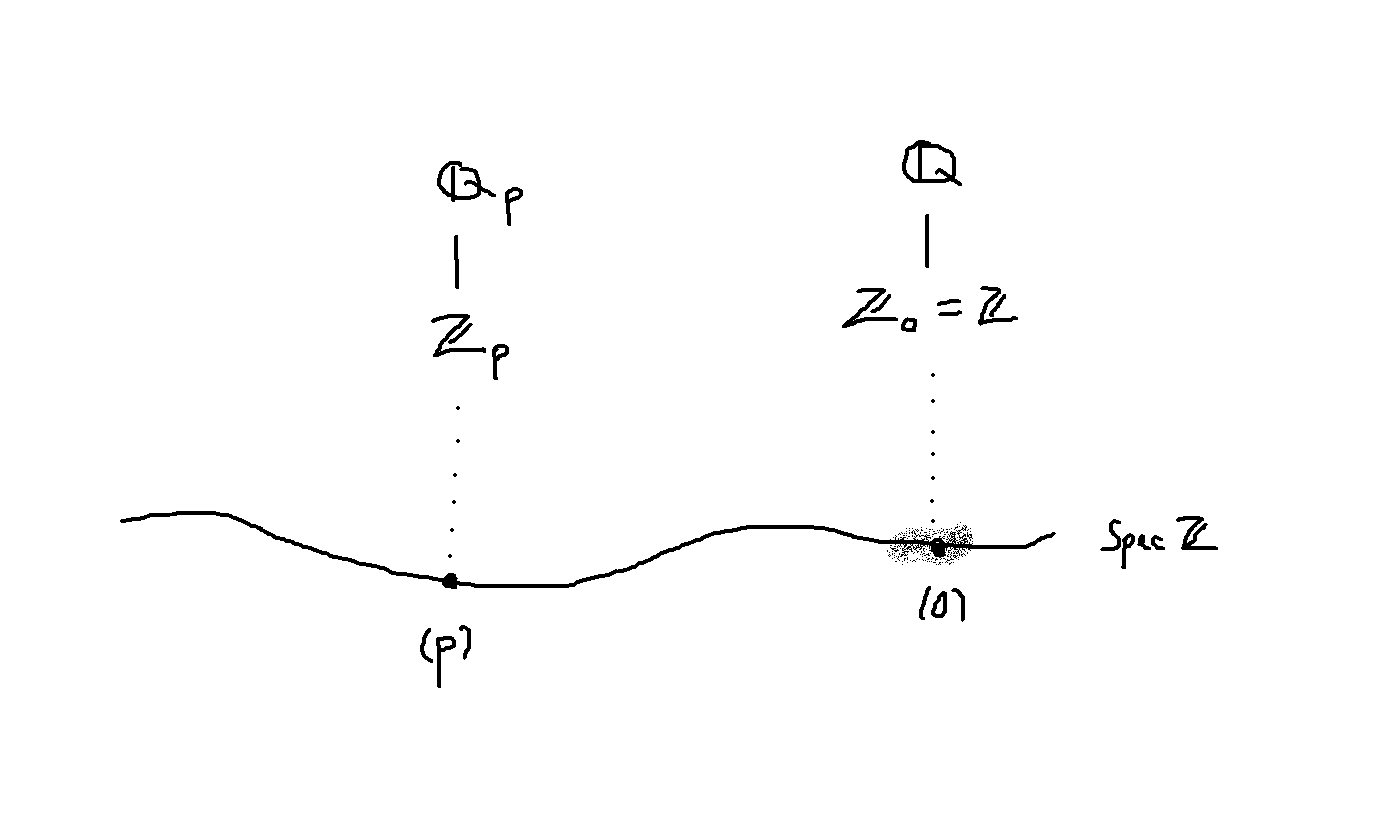
\includegraphics[width=\linewidth,height=\textheight,keepaspectratio]{Figures/places of Spec Z.png}
                                \caption{Local and global points of $\Spec \Z$}
                                \label{fig: local_and_global_points_of_Spec_Z}
                            \end{figure}
                    \end{remark}
                    \begin{definition}[Global models] \label{def: global_models}
                        We want our parametrising scheme, like $\Spec \Z$, to be one where the infinitestimal neighbourhoods (i.e. formal completions) around correspond to spectra of complete discrete valuation rings (for instance, the infinitestimal neighbourhoods $\Spf \Z_p$ around the points $(p) \in |\Spec \Z|$ correspond uniquely to the affine schemes $\Spec \Z_p$), which essentially means we want . We also want $S$ to be connected so that any residue field at a generic point would automatically be the function field of $S$.
                        
                        Let $S$ be base scheme satisfying the above conditions and let $K_0$ be its function field. Then, a \textbf{global model} for an algebraic scheme $X_0$ over $K_0$ shall be a flat and of finite type $S$-scheme $\bbX_0 \to S$. 
                    \end{definition}
                    \begin{remark}[Local-global compatibility] \label{remark: global_to_local_for_models}
                        
                    \end{remark}
                    
                    \begin{definition}[Pointed curves] \label{def: pointed_curves}
                        A \textbf{pointed elliptic curve} is a \textit{finitely presented} and \textit{proper} global model:
                            $$\bbE_0 \to S$$
                        with a distinguised so-called unit section $o_{\bbE_0}: S \to \bbE_0$ of one of the following:
                            \begin{itemize}
                                \item an elliptic curve over a place of $S$,
                                \item a projective nodal cubic curve over a place of $S$ (cf. \cite[\href{https://stacks.math.columbia.edu/tag/0C46}{Tag 0C46}]{stacks}), or
                                \item a projective cuspidal cubic curve over a place of $S$ (a point is a cusp if it corresponds to a non-splitting prime with inertial degree $2$; cf. definition \ref{def: ramification_indices}). 
                            \end{itemize}
                        A fibre of the first kind is said to be over a place of \textbf{good reduction}, whereas fibres over places of the second and third kind are said to be of \textbf{bad reduction}, as one ends up with singularities at those places.
                    \end{definition}
        
        \subsection{Moduli spaces of higher-dimensional abelian varieties; Shimura varieties}
            In a toungue-in-cheek manner, one might say that elliptic curves are nothing but abelian varieties of dimension $1$. One would not be in saying so, but in describing elliptic curves that way, one masks too many important aspects of these objects. This point of view is not entirely myopic and overly simplistic, however, since it does lead to a very fundamental question: do moduli spaces of higher-dimensional abelian varieties admit reasonable descriptions ? To answer this, let us note beforehand that elliptic curves are more than just $1$-dimensional abelian varieties: they admit \textbf{P}olarisations, \say{interesting} \textbf{E}ndomorphism rings, and \textbf{L}evel structures. As moduli stacks of elliptic curves with these extra structures taken into consideration behave quite well, geometrically, speaking, it thus makes sense to consider moduli spaces of abelian varieties that admitting these structures, so-called \textbf{\textit{PEL}-type abelian varieties} (note that elliptic curves admit polarisations trivially, as their automorphism groups - assuming the base field is of characteristic $p \not = 2, 3$ - are isomorphic to $\Z/n\Z$ for $n \in \{2, 4, 6\}$, i.e. finite). 
            
            \subsubsection{The geometry of abelian varieties}
                \begin{definition}[Abelian varieties] \label{def: abelian_varieties}
                    Fix a base scheme $S$. An \textbf{abelian $S$-scheme} is a group $S$-scheme that is smooth, proper, and geometrically connected. An abelian scheme over a field is \textit{a priori} an algebraic variety (in the sense of definition \ref{def: varieties}), so we shall refer to it as an \textbf{abelian variety}.
                \end{definition}
                This might seem like a rather stupid definition: abelian schemes sound like they should be abelian groups in the category of schemes, so why have we not just declared that every abelian group internal to $\Sch_{/S}$ is an abelian scheme ? The reason is two-fold:
                    \begin{enumerate}
                        \item By requiring that our abelian varieties are smooth and proper, we ensure that the machineries of \'etale cohomology are applicable.
                        \item Abelian group objects in $\Sch_{/S}$ can be geometrically very pathological. For instance, the group scheme associating to any commutative $\F_p$-algebra $R$ (for some prime $p$) its group of $n^{th}$ roots of unity is certainly commutative ($\mu_n(R)$, after all, is necessarily a subgroup of $\Z/n\Z$), which is represented by the affine scheme $\Spec \F_p[\zeta]/(\zeta^n - 1)$, is not even smooth in general, as the associated Jacobian vanishses everywhere (cf. definition \ref{def: standard_smoothness}).
                    \end{enumerate}
                As for why we have required abelian schemes to be geometrically connected group schemes in addition to being smooth and proper, this is because we want to make sure that elliptic curves are special cases of abelian schemes (in fact, elliptic curves are precisely abelian schemes of dimension $1$). Additionally, we will see how the connectedness assumption will help us prove that abelian schemes are indeed commutative group schemes.
                
                \begin{remark}[Basic geometric facts about abelian varieties] \label{remark: geometry_of_abelian_varieties}
                    \noindent
                    \begin{itemize}
                        \item \textbf{(Stability under base change):} If $A \to S$ is any ablian scheme and $S' \to S$ is an arbitrary morphism then $A' \cong S' \x_S A$ will also be an abelian scheme, albeit over $S'$ instead of $S$ this time. The proof of this assertion is identical to the argument presented in \ref{remark: moduli_of_elliptic_curves_disambiguations}.
                        \item \textbf{(Moduli stacks of abelian schemes):} For every fixed base scheme $S$, there exists a natural category of abelian $S$-schemes, wherein:
                            \begin{itemize}
                                \item the objects are abelian $S$-schemes, and
                                \item the morphisms are group scheme homomorphisms over $S$.
                            \end{itemize}
                        We will denote it by $(\calM_{n \geq 1})_{/S}$ (where the \say{$n \geq 1$} suggests that abelian of dimensions possibly higher than $1$ are also included); we choose this notation instead of $\Ab(S)$ to avoid confusing abelian schemes with abelian groups internal to schemes. Interestingly, not only is this a full subcategory of the category spanned by (smooth, proper, and geometrically connected) group schemes over $S$, but it is also fibred (in groupoids) over $\Sch_{/S}$ via the evident forgetful functor: the pullback functors between the fibres are simply given by fibred products. Furthermore, the aforementioned fibration:
                            $$(\calM_{n \geq 1})_{/S} \to \Sch_{/S}$$
                        satisfies Zariski, \'etale, fppf, and fpqc descent. 
                        
                        Now, for reasons similar to those discussed in remark \ref{remark: categories_of_elliptic_curves}, we will actually be more interested in the core of the category of abelian $S$-schemes, which we shall denote by $(\calM_{n \geq 1})_{/S}^{\circ}$. This category is (tautologically) fibred in groupoids over $\Sch_{/S}$, and later on, we shall show that certain subcategories of it admits meaningful geometric interpretations.
                        \item \textbf{(Integrality):}
                    \end{itemize}
                \end{remark}
                
                \begin{theorem}[Rigidity of proper flat families] \label{theorem: rigidity_theorem_1}
                    Let $\pi: X \to S$ be a flat and proper morphism of schemes whose local $0^{th}$ cohomologies are all isomorphic to the corresponding residue fields, i.e.:
                        $$\forall s \in |S|: H^0(X_s, \calO_{X_s}) \cong \kappa_s$$
                    Then:
                        \begin{enumerate}
                            \item the canonical map $\pi^{\sharp}: \calO_S \to \pi_*\calO_X$ will be an isomorphism, and
                            \item if $f: S' \to S$ is an affine-schematic morphism and if $\pi': X' \to S'$ is any morphism making the following diagram commutative:
                                $$
                                    \begin{tikzcd}
                                    	{X'} & X \\
                                    	{S'} & S
                                    	\arrow["f", from=2-1, to=2-2]
                                    	\arrow["\pi", from=1-2, to=2-2]
                                    	\arrow["{\pi'}"', from=1-1, to=2-1]
                                    	\arrow[from=1-1, to=1-2]
                                    \end{tikzcd}
                                $$
                            then $\pi': X' \to S'$ shall be constant.
                        \end{enumerate}
                \end{theorem}
                    \begin{proof}
                        \noindent
                        \begin{enumerate}
                            \item 
                            \item 
                        \end{enumerate}             
                    \end{proof}
                \begin{corollary} \label{coro: rigidity_theorem_2}
                    Let $\pi_1: X \to S$ be a flat and proper morphism of schemes whose local $0^{th}$ cohomologies are all isomorphic to the corresponding residue fields, i.e.:
                        $$\forall s \in |S|: H^0(X_s, \calO_{X_s}) \cong \kappa_s$$
                    Additionally, let $\pi_2: Y \to S$ be a separated map fitting into the following commutative diagram:
                        $$
                            \begin{tikzcd}
                            	X && Y \\
                            	& S
                            	\arrow["{\pi_1}"', from=1-1, to=2-2]
                            	\arrow["{\pi_2}", from=1-3, to=2-2]
                            	\arrow["f", from=1-1, to=1-3]
                            \end{tikzcd}
                        $$
                    Suppose now that $f: X \to Y$ is such that the fibre $f_s: X_s \to Y_s$ is constant for some fixed $s \in |S|$. Then, the restriction of $f: X \to Y$ to the connected component of the given point $s \in |S|$ will also be constant.
                \end{corollary}
                    \begin{proof}
                        
                    \end{proof}
                \begin{corollary}[Abelian schemes are abelian groups] \label{coro: abelian_schemes_are_abelian_groups}
                    Abelian schemes are abelian group objects in schemes.
                \end{corollary}
                    \begin{proof}
                        
                    \end{proof}
                    
            \subsubsection{The arithmetic of abelian varieties}
                \paragraph{Polarisations}
                    Let us first take a look at the moduli stack of polarised schemes. For that, however, we will need to say what it means for a line bundle on a scheme to be relatively ample beforehand.
                    
                    The following definition is actually not the most general one (cf. \cite[\href{https://stacks.math.columbia.edu/tag/01VG}{Tag 01VG}]{stacks}), but since abelian schemes are proper by definition, and most base schemes in arithmetic geometry are Noetherian anyway (in fact, most of the time one will simply be working over the spectrum of a field or a very topologically \say{nice} ring like $\Z$ or $\Z_p$), this notion of relative ampleness will suffice.
                    \begin{definition}[Relatively ample line bundles] \label{def: relatively_ample_line_bundles}
                        Let $\pi: X \to S$ be a morphism of schemes, and let $\calL$ be an invertible line bundle over $\calO_{X/S}$. This is said to be \textbf{$\pi$-relatively ample} if and only if:
                            \begin{itemize}
                                \item the base scheme $S$ is Noetherian,
                                \item the structural morphism $\pi: X \to S$ is proper, and
                                \item there exists $s \geq 0$ such that for all $\calF \in \Coh(X_{/S})$, all the higher cohomologies of $\calF \tensor_{\calO_{X/S}} \calL^{\tensor r}$ vanish for $r \geq s$, i.e.:
                                    $$\exists s \geq 0: \forall i > 0: \forall r \geq s: H^i(X_{/S}, \calF \tensor \calL^{\tensor r}) \cong 0$$
                            \end{itemize}
                    \end{definition}
                    \begin{remark}[Base-changing ample line bundles] \label{remark: base_changing_ample_line_bundles}
                        Let $S$ be a Noetherian base scheme, let $\pi: X \to S$ be a proper morphism, and let $f: S' \to S$ be a morphism of finite presentation. Next, consider the following pullback square:
                            $$
                                \begin{tikzcd}
                                	{X'} & X \\
                                	{S'} & S
                                	\arrow["g", from=1-1, to=1-2]
                                	\arrow["{\pi'}"', from=1-1, to=2-1]
                                	\arrow["\pi", from=1-2, to=2-2]
                                	\arrow["f", from=2-1, to=2-2]
                                	\arrow["\lrcorner"{anchor=center, pos=0.125}, draw=none, from=1-1, to=2-2]
                                \end{tikzcd}
                            $$
                        Also, suppose that $\calL$ is a $\pi$-relatively ample line bundle on $X/S$. Now, note that because $f: S' \to S$ is of finite presentation, $\calO_{S'}$ has to be coherent as a $\calO_S$-module, and hence $\calO_{X'}$ is coherent over $\calO_X$ as well. This implies, via the ampleness assumption on $\calL$, that for all coherent $\calO_{X'}$-modules $\calF'$, there exists $s \geq 0$ such that:
                            $$\forall i' > 0: \forall r' \geq s': H^i\left(X'_{/S'}, \calF' \tensor_{\calO_{X'}} \left(\calL^{\tensor r'} \tensor_{\calO_X} \calO_{X'}\right)\right) \cong 0$$
                        This tells us that the obvious base change $g^*\calL \cong \calL \tensor_{\calO_X} \calO_{X'}$ is indeed $\pi'$-relatively ample.
                    \end{remark}
                    
                    We can now define polarisations on schemes:
                    \begin{definition}[Polarisations] \label{def: polarisations}
                        Let $S$ be a Noetherian base scheme and consider a pullback square of the following form:
                            $$
                                \begin{tikzcd}
                                	{X'} & X \\
                                	{S'} & S
                                	\arrow["g", from=1-1, to=1-2]
                                	\arrow["{\pi'}"', from=1-1, to=2-1]
                                	\arrow["\pi", from=1-2, to=2-2]
                                	\arrow["f", from=2-1, to=2-2]
                                	\arrow["\lrcorner"{anchor=center, pos=0.125}, draw=none, from=1-1, to=2-2]
                                \end{tikzcd}
                            $$
                        wherein $\pi: X \to S$ and is flat, proper, and of finite presentation (and hence so is $\pi': X' \to S'$). If $\calL$ and $\calL'$ are relatively ample line bundles on $X/S$ and $X'/S'$ respectively, then one says that they define a \textbf{polarisation between $X/S$ and $X'/S'$} if and only if:
                            $$\calL' \cong g^*\calL$$
                    \end{definition}
                    \begin{remark}[Moduli stackss of polarised schemes] \label{remark: moduli_stacks_of_polarisations}
                        There is a natural fppf-stack of polarised flat proper schemes, which is in fact a substack of the relative Picard stack over $S$, which, we recall, classifies line bundles over $S$-schemes. Specifically, this new fppf-stack, which we will denote by $\Sch_{/S}^{\pol}$, is the restriction of the Picard stack down onto the subcategory of $\Sch_{/S, \fppf}^{\petit}$ spanned by schemes which are flat, proper, and of finite presentation over $S$.
                        
                        Actually, because the base change of ample line bundles along arbitrary morphisms of finite presentation remains ample, $\Sch_{/S}^{\pol}$ also satisfies Zariski, \'etale, and fpqc descent.
                    \end{remark}
                    \begin{remark}[Polarised abelian schemes] \label{remark: moduli_stacks_of_polarisations_on_abelian_schemes}
                        Abelian schemes are smooth and proper by definition, so they span a (non-full) subcategory of the category of schemes which are flat, proper, and of finite presentation over a given base scheme $S$. Should $S$ be Noetherian in addition, one can subsequently construct a natural category of polarised abelian schemes over $S$, which is fibred over $\Sch_{/S}^{\petit}$. By taking the core of this category, one then obtains a moduli space:
                            $$(\Alg\Spc_{/S}^{\pol})^{\circ} \to \Sch_{/S}^{\petit}$$
                        of polarised abelian schemes over $S$. Then, by combining remarks \ref{remark: geometry_of_abelian_varieties} and \ref{remark: moduli_stacks_of_polarisations}, one can show that this moduli space satisfies Zariski, \'etale, fppf, and fpqc descent.
                    \end{remark}
                    
                    \begin{proposition}[Some geometric properties of moduli stacks of polarised schemes] \label{prop: geometric_properties_of_moduli_stacks_of_polarised_schemes}
                        Fix a Noetherian base scheme $S$. 
                            \begin{enumerate}
                                \item There exists a natural and obvious extension of the moduli stack:
                                    $$(\Sch_{/S}^{\pol})^{\circ} \to \Sch_{/S, \fppf}$$
                                to a moduli stack:
                                    $$(\Alg\Spc_{/S}^{\pol})^{\circ} \to \Alg\Spc_{/S, \fppf}^{\petit}$$
                                of \textbf{polarised algebraic spaces}, which is fibred in groupoids over the \textit{small} base category spanned by algebraic spaces fppf over $S$.
                                \item The diagonal:
                                    $$\Delta_{(\Alg\Spc_{/S}^{\pol})^{\circ}}: (\Alg\Spc_{/S}^{\pol})^{\circ}\to (\Alg\Spc_{/S}^{\pol})^{\circ} \x_S (\Alg\Spc_{/S}^{\pol})^{\circ}$$
                                is representable (cf. definition \ref{def: affine_schematic}) as a morphism of stacks on $\Alg\Spc_{/S, \fppf}^{\petit}$. Furthermore, it is separated and of finite presentation.
                                \item As a $(2, 1)$-sheaf on $\Alg\Spc_{/S, \fppf}^{\petit}$, $(\Alg\Spc_{/S}^{\pol})^{\circ}$ preserves limits in $\Alg\Spc_{/S, \fppf}^{\petit}$. 
                            \end{enumerate}
                    \end{proposition}
                        \begin{proof}
                            \noindent
                            \begin{enumerate}
                                \item 
                                \item 
                                \item 
                            \end{enumerate}
                        \end{proof}
                
                \paragraph{Endomorphisms}
                
                \paragraph{Level structures}
            
            \subsubsection{PEL-type Shimura varieties}
                As it turns out, the space parametrising these abelian varieties are Shimura varieties, particularly so-called \textbf{PEL-type Shimura varieties}. These geometric objects are horrifyingly complicated to properly describe in details, however, so let us first take a look at an illustrative example. 
            
                Consider the (absolute) moduli space:
                    $$(\calM_{n = g}^{(d, N)})^{\circ} \to \Sch_{/\Spec \Z[1/N]}$$
                fibred over $\Sch_{/\Spec \Z[1/N]}$, whose fibres over objects $S \in \Sch_{/\Spec \Z[1/N]}$ are the cores of the categories of abelian $S$-schemes $A_{/S}$ which:
                    \begin{itemize}
                        \item are of some fixed dimension $n = g \geq 0$,
                        \item admit a level-$N$ structure $\phi_N: (\Z/N\Z)^{\oplus 2g} \cong A_{/S}[N]$,
                        \item have a polarisation of degree $d^2$.
                    \end{itemize}
    
        \chapter{Algebraic topology and higher category theory}
    \begin{abstract}
        
    \end{abstract}
    
    \minitoc
    
    \section{\texorpdfstring{$n$}{}-operads and \texorpdfstring{$n$}{}-categories}
        \subsection{Monoidal categories; enrichments}
            \subsubsection{Classical monoidal categories}
                \begin{definition}[Monoidal categories] \label{def: monoidal_categories}
                    A monoidal category is a quintuple $(\V, \tensor, 1, \alpha, (\lambda, \rho))$ of:
                        \begin{enumerate}
                            \item a category $\V$;
                            \item a bifunctor $\tensor: \V \x \V \to \V$;
                            \item a distinguished object $1 \in \V$ - called the \textbf{unit} - which we shall view as a functor $\eta: \pt \to \V$ from the terminal category;
                            \item a natural isomorphism of functors - called the \textbf{associator} - as follows:
                                $$
                                    \begin{tikzcd}
                                    	{(\V \x \V) \x \V} && {\V \x (\V \x \V)} \\
                                    	\\
                                    	{\V \x \V} && {\V \x \V} \\
                                    	& \V
                                    	\arrow["{\tensor \x \id_{\V}}"', from=1-1, to=3-1]
                                    	\arrow["\tensor"', from=3-1, to=4-2]
                                    	\arrow["\tensor", from=3-3, to=4-2]
                                    	\arrow["{\id_{\V} \x \tensor }", from=1-3, to=3-3]
                                    	\arrow["\cong", from=1-1, to=1-3]
                                    	\arrow[""{name=0, anchor=center, inner sep=0}, "{(- \tensor -) \tensor -}"{description}, from=1-1, to=4-2]
                                    	\arrow[""{name=1, anchor=center, inner sep=0}, "{- \tensor (- \tensor -)}"{description}, from=1-3, to=4-2]
                                    	\arrow["\alpha", shorten <=26pt, shorten >=26pt, Rightarrow, from=0, to=1]
                                    \end{tikzcd}
                                $$
                            \item natural isomorphisms $\lambda$ and $\rho$ - known, respectively, as the \textbf{left and right-unitors} - as follows:
                                $$
                                    \begin{tikzcd}
                                    	{\V \x \pt} & {\V \x \V} & {\pt \x \V} \\
                                    	\V & \V & \V
                                    	\arrow["{\tensor}"{description}, from=1-2, to=2-2]
                                    	\arrow["{\eta \x \id_{\V}}"', from=1-3, to=1-2]
                                    	\arrow["{\id_{\V} \x \eta}", from=1-1, to=1-2]
                                    	\arrow["{\id_{\V}}"', from=2-1, to=2-2]
                                    	\arrow["{\pr_1}"', from=1-1, to=2-1]
                                    	\arrow["{\pr_2}", from=1-3, to=2-3]
                                    	\arrow["{\id_{\V}}", from=2-3, to=2-2]
                                    	\arrow["\lambda"', shorten <=13pt, shorten >=13pt, Rightarrow, from=1-2, to=2-1]
                                    	\arrow["\rho", shorten <=13pt, shorten >=13pt, Rightarrow, from=1-2, to=2-3]
                                    \end{tikzcd}
                                $$
                            (note that the functors $\pr_1: \V \x \pt \to \V$ and $\pr_2: \pt \x \V \to \V$ are equivalences \textit{a priori}, thanks to the universal property of the terminal objects and that of products).
                        \end{enumerate}
                    
                \end{definition}
                \begin{definition}[Lax-monoidal categories] \label{def: lax_monoidal_categories}
                    Let $(\V, \tensor, 1, \alpha, (\lambda, \rho))$ a quintuple as in definition \ref{def: monoidal_categories}, but now, suppose that $\alpha: (- \tensor -) \tensor - \to - \tensor (- \tensor -)$ is a non-invertible $2$-cell. Then, this quintuple will define a so-called \textbf{lax-monoidal category} if and only if 
                \end{definition}
                \begin{definition}[Non-unital monoidal categories]
                    
                \end{definition}
                
                \begin{definition}[Braidings and symmetries] \label{def: braided_and_symmetric_monoidal_categories}
                    
                \end{definition}
                
            \subsubsection{Categories enriched over monoidal categories; 2-categories}
            
            \subsubsection{Unbiased monoidal categories}
        
        \subsection{Operads and coloured operads}
        
        \subsection{Weak \texorpdfstring{$n$}{}-categories}
            \subsubsection{Globular operads}
            
            \subsubsection{The many definitions of weak \texorpdfstring{$n$}{}-categories}
            
    \section{\texorpdfstring{$(\infty, 1)$}{}-categories and \texorpdfstring{$\infty$}{}-topoi}
    
    \section{Monoidal \texorpdfstring{$(\infty, 1)$}{}-categories and \texorpdfstring{$(\infty, 2)$}{}-categories}
        \subsection{Monoidal \texorpdfstring{$(\infty, 1)$}{}-categories}
            \begin{convention}
                Until the end of this subsection, the term \say{$\infty$-category} shall be used in place of \say{$(\infty, 1)$-category}, barring extreme prejudices.
            \end{convention}
        
            \subsubsection{Monoidal structures; algebra objects}
                Monoidal categories (cf. definition \ref{def: monoidal_categories}) are categories $\V$ equipped with a bifunctor $\tensor: \V \x \V \to \V$ satisfying axioms which help us ensure that (finite) \say{tensor products} of objects in $\V$ with one another would behave in a similar manner to tensor products of modules. Notably, these \say{tensor products} are only defined up to isomorphisms; in other words, one says that the bifunctor $\tensor$ is subjected to certain \say{coherence conditions}. Now, what if we would like a theory of monoidal categories wherein said coherence conditions admit coherence conditions of their own, e.g. isomorphisms between say, $x \tensor y$ amd $y \tensor x$ form not a set\footnote{Let us ignore set-theoretic issues for now.} but rather, a groupoid whose objects are these isomorphisms and whose (invertible) $1$-cells are \say{$2$-isomorphisms} between these isomorphisms (e.g. concretely, one might think of the $2$-category $(1\-\Cat_2, \x, \pt)$ of small $1$-categories with its canonical monoidal structure given by finite products: products $\C \x \D$ are defined up to equivalences of categories, but one may also speak of invertible natural transformations between these equivalences of categories) ? Of course, one can write down these higher coherence conditions by hand, but given the complexity of the definition of monoidal $1$-categories alone (cf. definition \ref{def: monoidal_categories}), it might prove prudent to seek out an alternative method. Moreover, given how $\infty$-categories are \say{spaces} in which equivalences are only specified up to an infinite number of higher coherence constraints, simply trying to specify these coherence conditions might not be so wise a thing to attempt after all.
                
                To that end, let us begin our construction of monoidal $\infty$-categories with an observation.
                \begin{remark}[Monoidal structures as op-fibrations] \label{remark: monoidal_op_fibrations}
                    Recall how for $R$ a commutative ring, the binary tensor product $M \tensor_R N$ of two $R$-modules $M$ and $N$ is defined to be the universal $R$-module such that for every pair of $R$-bilinear maps $M \x N \to P$ and $M \x N \to M \tensor_R N$, there exists a unique $R$-linear map $M \tensor_R N \to P$ making the following diagram commute:
                        $$
                            \begin{tikzcd}
                            	{M \x N} & {M \tensor_R N} \\
                            	& P
                            	\arrow[from=1-1, to=1-2]
                            	\arrow[dashed, from=1-2, to=2-2]
                            	\arrow[from=1-1, to=2-2]
                            \end{tikzcd}
                        $$
                    One would then show that binary tensor products are nothing special: in fact, one can re-iterate the construction an arbitrary (but finite!) number of times to get $n$-ary tensor products $\bigotimes_{i = 1}^n M_i$ that satisfy a similar kind of universal property; one can also show that the $0$-fold tensor product exists as the zero module. 
                    
                    At this point, we might suspect that the endowment of finite tensor products to some category $\V$ might be some functorial process $\simp^{\op} \to \V^{\tensor}$ whereby one associates to some given enumerating sequence of indices $[n] \in \simp^{\op}$ a sequence $\{x_1, x_2, ..., x_n\} \in \V^{\tensor}$ of objects of $\V$, which should be thought of as diagrams $[n] \to \V$.
                \end{remark}
                
                We have thus come to the notion of monoidal ($1$-)op-fibrations:
                \begin{definition}[Monoidal op-fibrations] \label{def: monoidal_op_fibrations}
                    Let $(\V, \tensor, \1)$ be a monoidal category. Then, let us associate to it a $1$-functor:
                        $$\V^{\tensor}: \simp^{\op} \to 1\-\Cat_1$$
                    subjected to the following constraints:
                        \begin{enumerate}
                            \item $\V^{\tensor}$ ought to preserve the terminal object $[0] \in \simp^{\op}$, i.e.:
                                $$\V^{\tensor}([0]) \cong \pt$$
                            \item For all $n \geq 1$, the following natural $n$-tuple of natural arrows in $\simp^{\op}$:
                                $$[n] \to [1]: \left((i \to i + 1) \mapsto (0 \to 1)\right) \: (\forall i \in [n])$$
                            defines an equivalence:
                                $$\V^{\tensor}([n]) \cong \V^{\tensor}([1])^n$$
                        \end{enumerate}
                \end{definition}
                The functor $\V^{\tensor}$ shall - in time - be thought of as the monoidal structure on $\V$. This, however, is a somewhat non-trivial fact, along with the following, which establishes some descent-theoretic coherence properties of monoidal structures as in definition \ref{def: monoidal_op_fibrations}. 
                \begin{proposition}
                    Let $(\V, \tensor, \1)$ be a monoidal category and let us assume the Axiom of Choice (which is equivalent to every fibred category having a cleavage; cf. \cite[Definition 3.9]{vistoli_descent}). Then, the canonically associated functor (as in definition \ref{def: monoidal_op_fibrations}):
                        $$\V^{\tensor}: \simp^{\op} \to 1\-\Cat_1$$
                    defines a coCartesian fibration:
                        $$p^{\tensor}: 1\-\Cat_1 \to \simp^{\op}$$
                    and vice versa.
                \end{proposition}
                    \begin{proof}
                        Fix a category $V_n \in 1\-\Cat$ such that $p^{\tensor}(V_n) \cong [n]$ (i.e. a section over $[n] \in \simp^{\op}$) along with a pair of arbitrary arrows $\varphi: V_n \to V$ and $\psi: V_n \to V'$ and inducing the following commutative diagram in $\simp^{\op}$ wherein $h: p^{\tensor}(V) \to p^{\tensor}(V')$ is arbitrary:
                            $$
                                \begin{tikzcd}
                                    p^{\tensor}(V') \arrow[rd, "h"'] \arrow[rrd, "p^{\tensor}(\psi)", bend left] &                                                  &       \\
                                                                                                                 & p^{\tensor}(V) \arrow[r, "p^{\tensor}(\varphi)"] & {[n]}
                                \end{tikzcd}
                            $$
                        The definition of the category $\simp$ can then be made use of, specifically to realise that $p^{\tensor}(V) \cong [m]$ and $p^{\tensor}([m'])$ for $m, m' \in \N$ such that $m' \geq m \geq n$. Definition \ref{def: monoidal_op_fibrations} and the universal property of products (note that because $p^{\tensor}(V) \cong [m]$ and $p^{\tensor}([m'])$, we have $V \cong \V^{\tensor}([1])^m$ and $V' \cong \V^{\tensor}([1])^{m'}$) then ensures that there exists an arrow $\eta: V' \to V$ making the following diagram commute:
                            $$
                                \begin{tikzcd}
                                    V' \arrow[rd, "\eta"', dashed] \arrow[rrd, "\psi", bend left] &                                                  &       \\
                                                                                                                 & V \arrow[r, "\varphi"] & {V_n}
                                \end{tikzcd}
                            $$
                            
                        The converse assertion comes directly from the fact that given the Axiom of Choice, every fibred category admits a cleavage.
                    \end{proof}
                
            \subsubsection{Monoidal \texorpdfstring{$(\infty, 1)$}{}-categories as coCartesian fibrations}
            
            \subsubsection{Universal constructions in monoidal \texorpdfstring{$(\infty, 1)$}{}-categories}
        
        \subsection{\texorpdfstring{$(\infty, 2)$}{}-categories}
        
    \section{Algebraic K-theory}
    
        \chapter{Homological and homotopical algebra}
    \begin{abstract}
        
    \end{abstract}
    
    \minitoc
    
    \section{\textit{Hors d'oeuvres}: Classical homological algebra}
        \begin{convention}
            Throughout this section we will be working with ordinary $1$-categories, not $(\infty, 1)$-categories. However, we will still try to phrase as many definitions and proofs in a manner that would generalise more or less trivially to the setting of $\infty$-categories.
        \end{convention}
    
        \subsection{Additive categories, abelian categories, everything in between and beyond!}
            \subsubsection{Abelian categories: the backdrop for homological algebra}
                \paragraph{Zero objects and zero morphisms; (co)kernels}
                    Let us first perform some analysis of zero objects and (finite) biproducts in general categories wherein they exist. First up is the definition:
                    \begin{definition}[Zero objects] \label{def: zero_objects}
                        A \textbf{zero object} (in any category) is an object satisfying both the universal properties of an initial and terminal object.
                    \end{definition}
                    
                    \todo{Add info about zero morphisms}
                    
                    \begin{definition}[(Co)kernels] \label{def: (co)kernels}
                        Within a category with zero objects $0$, the \textbf{kernel} of an arrow $f: x \to y$, should it exist, shall be the following pulback:
                            $$
                                \begin{tikzcd}
                                	{\ker f} & 0 \\
                                	x & y
                                	\arrow["\1", from=1-2, to=2-2]
                                	\arrow["f", from=2-1, to=2-2]
                                	\arrow[from=1-1, to=2-1]
                                	\arrow[from=1-1, to=1-2]
                                	\arrow["\lrcorner"{anchor=center, pos=0.125}, draw=none, from=1-1, to=2-2]
                                \end{tikzcd}
                            $$
                        Dually, the \textbf{cokernel} of an arrow $f: x \to y$ (and again, should it exist) shall be the following pushout:
                            $$
                                \begin{tikzcd}
                                	x & y \\
                                	0 & {\coker f}
                                	\arrow["f", from=1-1, to=1-2]
                                	\arrow["\2"', from=1-1, to=2-1]
                                	\arrow[from=1-2, to=2-2]
                                	\arrow[from=2-1, to=2-2]
                                	\arrow["\lrcorner"{anchor=center, pos=0.125, rotate=180}, draw=none, from=2-2, to=1-1]
                                \end{tikzcd}
                            $$
                    \end{definition}
                    \begin{remark}[(Co)kernels as (co)equalisers] \label{remark: (co)kernels_as_(co)equalisers}
                        Let $x, y$ be objects of some category with zero objects $0$. Thanks to the universal property of zero objects, namely thanks to the fact that there would always exist unique morphisms $\1: 0 \to y$ and $\2: x \to 0$ making the following diagram commute:
                            $$
                                \begin{tikzcd}
                                	{} & 0 \\
                                	x & y
                                	\arrow["{0_{x, y}}"', from=2-1, to=2-2, dashed]
                                	\arrow["\1", from=1-2, to=2-2]
                                	\arrow["\2", from=2-1, to=1-2]
                                \end{tikzcd}
                            $$
                        Every such diagram and every arrow $f: x \to y$ thus give rise a pair of parallel arrows, namely $f, 0_{x, y}: x \toto y$. Now, the claim is that the limit/equaliser of this diagram is precisely $\ker f$. To prove this, simply consider the following commutative diagram:
                            $$
                                \begin{tikzcd}
                                	& {\ker f} & x \\
                                	& x & y \\
                                	0
                                	\arrow["f", from=1-3, to=2-3]
                                	\arrow[from=1-2, to=1-3]
                                	\arrow["\lrcorner"{anchor=center, pos=0.125}, draw=none, from=1-2, to=2-3]
                                	\arrow["{0_{x, y}}", from=2-2, to=2-3]
                                	\arrow[from=1-2, to=2-2]
                                	\arrow["\1"{description}, from=3-1, to=2-2]
                                	\arrow["\1"', from=3-1, to=2-3]
                                	\arrow["\2"', from=1-2, to=3-1]
                                \end{tikzcd}
                            $$
                    \end{remark}
                
                \paragraph{Biproducts}
                    Another notion that will come up often in tandem with that of zero objects is the idea of biproducts:
                    \begin{definition}[Biproducts] \label{def: biproducts}
                        A \textbf{biproduct} (in any category) is an object satisfying both the universal properties of a product and a coproduct.
                    \end{definition}
                    \begin{remark}
                        Note that zero objects and biproducts are particular instances of so-called \textbf{bilimits}. 
                    \end{remark}
                    
                    We note that having zero objects is not a sufficient condition for having (finite) biproducts. Consider the following example:
                    \begin{example}[Having zero objects does not imply having having biproducts] \label{example: zero_objects_do_not_imply_biproducts}
                        In the category ${}^{\{*\}/}\Top$ of \textit{pointed} topological spaces and continuous functions, the identity $\id_{\{*\}}: \{*\} \to \{*\}$ on the one-point space $\{*\}$ (i.e. the distinguished point of the one-point space) is a zero object. Clearly, $\id_{\{*\}}: \{*\} \to \{*\}$ is the initial object in ${}^{\{*\}/}\Top$. As for why it is the final object in ${}^{\{*\}/}\Top$, consider firstly the following commutative triangle in $\Top$ (i.e. the following morphism from $x: \{*\} \to X$ to $\id_{\{*\}}: \{*\} \to \{*\}$):
                            $$
                                \begin{tikzcd}
                                	\{*\} \\
                                	X & \{*\}
                                	\arrow["x"', from=1-1, to=2-1]
                                	\arrow["{\id_{\{*\}}}", from=1-1, to=2-2]
                                	\arrow["{!}", from=2-1, to=2-2]
                                \end{tikzcd}
                            $$
                        wherein $X$ is any (pointed) topological space; note that any point $x \in X$ naturally induces a continuous map $x: \{*\} \to X$; also, there exists, for all spaces $X$, a natural and unique surjection $!: X \to \{*\}$ sending every element of $X$ to the unique element of $\{*\}$ (it is indeed continuous, since the preimages of the two open subsets $\varnothing, \{*\} \in \Ouv(\{*\})$ under $!: X \to \{*\}$, being $\varnothing$ and $X$ respectively, are both open in $X$). This diagram tells you that there exists a natural and unique morphism from any $(x: \{x\} \to X) \in {}^{\{*\}/}\Top$ to $\id_{\pt}: \pt \to \pt$, or in other words, that $\id_{\{*\}}: \{*\} \to \{*\}$ is a terminal object in ${}^{\{*\}/}\Top$. 
                    \end{example}
                    Now, as pathological as this example might be, and as much as it might scare us, fear not, for ${}^{\{*\}/}\Top$ is not $\Ab$-enriched (simply note how there is not a good way to define the addition of two continuous morphisms with common domain and codomain)! Therefore, the example above should not concern us too much. In fact, being $\Ab$-enriched is a rather strong assumption, as we shall see through the following proposition:
                    \begin{proposition}[Criterion for having enough finite biporducts] \label{prop: finite_biproduct_criterion}
                        Let $\calA$ be an $\Ab$-enriched category with zero objects $0$ and all finite products. Then $\calA$ has all finite biproducts. 
                    \end{proposition}
                        \begin{proof}
                            As biproducts satisfy both the universal properties of products and coproducts, it shall suffice to show, that for all $x, y \in \calA$, $x \x y$ satisfies the universal property of a coproduct. This entails showing that there exist morphisms $x \to x \x y$ and $y \to x \x y$, and that the following diagram (wherein $x \x y \to z$ is unique) commutes for all $x \to z$ and $y \to z$:
                                $$
                                    \begin{tikzcd}
                                                                            & y \arrow[rdd, bend left] \arrow[d]                &   \\
                                        x \arrow[rrd, bend right] \arrow[r] & x \x y \arrow[rd, "\exists!" description, dashed] &   \\
                                                                            &                                                   & z
                                    \end{tikzcd}
                                $$
                                \begin{enumerate}
                                    \item By symmetry, it suffices to show that there exists a morphism $x \to x \x y$. 
                                    
                                    Now, by the universal property of zero objects (which implies that there exist unique morphisms $\2: x \to 0$ and $\1: 0 \to y$) the following diagram commutes:
                                        $$
                                            \begin{tikzcd}
                                                                                                   & 0 \arrow[d, "\1"] \\
                                                x \arrow[r, "{0_{x, y}}"', dashed] \arrow[ru, "\2"] & y                
                                            \end{tikzcd}
                                        $$
                                    From this, one infers that there exists the following diagram:
                                        $$
                                            \begin{tikzcd}
                                                x \arrow[r, "{0_{x, y}}", dashed] \arrow[d, "\id_x"'] & y \\
                                                x                                                     &  
                                            \end{tikzcd}
                                        $$
                                    which fits naturally into the following commutative diagram, thanks to the universal property of products:
                                        $$
                                            \begin{tikzcd}
                                            	x & y \\
                                            	x & {x \x y} & y \\
                                            	& x
                                            	\arrow["{0_{x, y}}", from=1-1, to=1-2]
                                            	\arrow["{\id_x}"', from=1-1, to=2-1]
                                            	\arrow[from=2-2, to=3-2]
                                            	\arrow[from=2-2, to=2-3]
                                            	\arrow["{\id_x}"', from=2-1, to=3-2]
                                            	\arrow["{\id_y}", from=1-2, to=2-3]
                                            	\arrow[dashed, from=1-1, to=2-2]
                                            \end{tikzcd}
                                        $$
                                    We have thus found a morphism  $x \to x \x y$.
                                    \item Now that we know there are natural maps $x \to x \x y \ot y$, consider a diagram of the following form, wherein $z$ is arbitrary:
                                        $$
                                            \begin{tikzcd}
                                                                                                        & y \arrow[d] \arrow[rdd, bend left] &   \\
                                                x \arrow[r] \arrow[rrd, bend right] & x \x y \arrow[rd, "\exists ?" description, dashed]   &   \\
                                                                                                        &                                                      & z
                                            \end{tikzcd}
                                        $$
                                    If we can show that the dashed arrow exists, then by the universal property of coproducts, we will have shown that $x \x y$ is a coproduct in $\calA$. To that end, note that every diagram $j_1: x \to z \ot y: j_2$ embeds naturally into the following commutative diagram, thanks to the universal property of products:
                                        $$
                                            \begin{tikzcd}
                                                x \x y \arrow[d, "\pr_1"', dashed] \arrow[r, "\pr_2", dashed] & y \arrow[d, "j_2"] \\
                                                x \arrow[r, "j_1"]                                            & z                 
                                            \end{tikzcd}
                                        $$
                                    Thanks to the crucial assumption that $\calA$ is $\Ab$-enriched, the diagram above induces the following morphism:
                                        $$j_1 \circ \pr_1 + j_2 \circ \pr_2: x \x y \to z$$
                                    We now claim that $\varphi := j_1 \circ \pr_1 + j_2 \circ \pr_2$ is the sought-for dashed arrow from the first diagram. To show that this is indeed the case, let us simply check that the resulting diagram actually commutes. For this, denote by $\iota_1: x \to x \x y \ot y: \iota_2$ the natural maps and consider the following:
                                        $$
                                            \begin{aligned}
                                                \varphi \circ \iota_1 & = (j_1 \circ \pr_1 + j_2 \circ \pr_2) \circ \iota_1
                                                \\
                                                & = j_1 \circ \pr_1 \circ \iota_1 + j_2 \circ \pr_2 \circ \iota_1
                                                \\
                                                & = j_1 \circ \id_x + j_2 \circ 0_{x, y}
                                                \\
                                                & = j_1 + 0_{x, x \x y}
                                                \\
                                                & = j_1
                                            \end{aligned}
                                        $$
                                    wherein $\pr_1 \circ \iota_1 = \id_x$ and $\pr_2 \circ \iota_1 = 0_{x, y}$ because we have shown in the previous step that the following diagram commutes:
                                        $$
                                            \begin{tikzcd}
                                                x \arrow[rd, "j_1" description] \arrow[rrd, "{0_{x, y}}", bend left] \arrow[rdd, "\id_x"', bend right] &                                               &   \\
                                                                                                                                                       & x \x y \arrow[r, "\pr_2"] \arrow[d, "\pr_1"'] & y \\
                                                                                                                                                       & x                                             &  
                                            \end{tikzcd}
                                        $$
                                    Likewise, one can show that:
                                        $$\varphi \circ \iota_2 = j_2$$
                                    There thus exists $\varphi: x \x y \to z$ making the following diagram commute:
                                        $$
                                            \begin{tikzcd}
                                                                                                       & y \arrow[d, "\iota_2"] \arrow[rdd, "j_2", bend left] &   \\
                                                x \arrow[r, "\iota_1"] \arrow[rrd, "j_1"', bend right] & x \x y \arrow[rd, "\exists \varphi"]                 &   \\
                                                                                                       &                                                      & z
                                            \end{tikzcd}
                                        $$
                                    \item Lastly, to show that the map $\varphi$ as above is unique, suppose to the contrary that it is not, i.e. there exists $\psi \not = \varphi$ making the diagram:
                                        $$
                                            \begin{tikzcd}
                                                                                                       & y \arrow[d, "\iota_2"] \arrow[rdd, "j_2", bend left] &   \\
                                                x \arrow[r, "\iota_1"] \arrow[rrd, "j_1"', bend right] & x \x y \arrow[rd, "\psi"]                 &   \\
                                                                                                       &                                                      & z
                                            \end{tikzcd}
                                        $$
                                    commute. The existence of such an arrow would imply that:
                                        $$\psi \circ \iota_1 = j_1 = \varphi \circ \iota_1$$
                                    and hence:
                                        $$(\psi - \varphi) \circ \iota_1 = \psi \circ \iota_1 - \varphi \circ \iota_1 = j_1 - j_1 = 0_{x, z}$$
                                    and because $\iota_1 \not = 0$, it must be the case that $\psi - \varphi = 0_{x, x \x y}$; thus, we have shown that $\psi = \varphi$, which contradicts the assumption that $\psi \not = \varphi$. The arrow $\varphi: x \x y \to z$ from the previous step is thus unique.
                                \end{enumerate}
                            We have therefore shown that every binary product in $\calA$ satisfies the universal property of a coproduct, which implies (via some elementary induction) that $\calA$ has all finite biproducts.
                        \end{proof}
                    
                \paragraph{Homological categories}
                    \begin{definition}[Additive and abelian categories] \label{def: AB_categories}
                        An \textbf{additive category} is an $\Ab$-enriched category with zero objects and finite biproducts.
                        
                        This notion is subsumed by those of:
                            \begin{enumerate}
                                \item \textbf{$\Ab$-enriched categories},
                                \item \textbf{pre-additive categories} (i.e. categories with zero objects),
                                \item \textbf{pseudo-abelian categories} (i.e. categories wherein all idempotent endomorphisms admit kernels and cokernels),
                            \end{enumerate}
                        and itself generalises the following notions:
                            \begin{enumerate}
                                \item \textbf{pre-abelian/$AB1$ categories} (i.e. additive categories admitting all kernels and all cokernels),
                                \item \textbf{abelian/$AB2$ categories} (i.e. pre-abelian categories wherein every monomorphism is a kernel and every epimorphism is a cokernel).
                            \end{enumerate}
                        The hierachy continues with even stronger notions:
                            \begin{enumerate}
                                \item An \textbf{$AB3$-category} is an $AB2$-category with all coproducts; dually, an \textbf{$AB3^*$-category} is an $AB2$-category with all products.
                                \item An \textbf{$AB4$-category} is an $AB3$-category wherein coproducts and monomorphisms commute; dually, an \textbf{$AB4^*$-category} is one wherein products and epimorphisms commute.
                                \item An \textbf{$AB5$-category} is an $AB3$-category wherein filtered colimits of exact sequences (i.e. chain complexes with vanishing homologies) remain exact; dually, an \textbf{$AB5^*$-category} is one wherein filtered limits of exact sequences remain exact.
                                
                                Additionally, a so-called \textbf{Grothendieck category} is a presentable $AB5$-category.
                                \item Lastly, an \textbf{$AB6$-category} is an $AB3$-category wherein products and filtered colimits commute; dually an \textbf{$AB6^*$-category} is one wherein coproducts commute with filtered limits.
                            \end{enumerate}
                    \end{definition}
                    
                    \begin{proposition}[$AB1$-categories are finitely (co)complete] \label{prop: AB1_categories_are_finitely_(co)complete}
                        Any $AB1$-category $\calA$ is simultaneously finitely complete and finitely cocomplete.
                    \end{proposition}
                        \begin{proof}
                            This is a straightforward consequence of the fact that one can construct finite (co)limits from finite pullbacks/pushouts and terminal/initial objects, and that having pullbacks/pushouts and terminal/initial objects implies having (co)products.
                        \end{proof}
                    
                    \begin{example}[Additive categories and so on] \label{examples: AB_categories}
                        \noindent
                        \begin{itemize}
                            \item \textbf{(Modules):}
                            \item \textbf{(Non-unital rings):}
                            \item \textbf{(A counter-example: free modules over PIDs that are not fields):}
                            \item \textbf{(An additive category that is not $AB2$):} Let $K$ be a locally compact complete (ultra)metric field (e.g. $\R, \bbC$, or finite extensions of $\Q_p$ or $\F_p(\!(t)\!)$, for some prime $p$) and consider the category $K\Ban$ of $K$-Banach spaces (i.e. $K$-vector spaces topologically complete with respect to a norm induced by the (ultra)metric on $K$) and bounded continuous $K$-linear transformations. We claim that epimorphisms in this category can fail to be cokernels, and hence $K\Ban$ fails to be $AB2$.
                            
                            First of all, for the sake of completeness, let us note that $K\Ban$ is $\Ab$-enriched: the enrichment is is given by the usual addition of continuous linear transformation, which preserves boundedness thereof, since either:
                                $$\|\varphi + \psi\| \leq \|\varphi\| + \|\psi\|$$
                            or:
                                $$\|\varphi + \psi\| \leq \max\{\|\varphi\|, \|\psi\|\}$$
                            and both right-hand sides are finite by the boundedness assumption on the morphisms $\varphi, \psi$ in $K\Ban$.
                            
                            Now, let $Z$ be a compact subspace of $K$ (e.g. compact intervals in $\R$, compact balls in $\bbC$, or $\Z_p$ in $\Q_p$) and consider the Banach $K$-algebra $C^0(X)$ of continuous $K$-valued functions on $Z$; this Banach $K$-algebra is a dense $K$-subalgebra of $L^1(Z)$, the Banach $K$-algebra of absolutely integrable $K$-valued functions on $Z$.
                            \item \textbf{(Sheaves of modules):} Let $\E$ be a topos and let $R$ be a ring object internal to $\E$. Then, the category $R\mod$ of left-$R$-modules will be a Grothendieck category, and likewise with $\mod_R$ and $R\mod_R$.
                        \end{itemize}
                    \end{example}
                    
                    \begin{example}[An important example: chain complexes] \label{example: chain_complexes}
                        In a category $\calA$ with zero objects $0$, a \textbf{chain complex}\footnote{You might also have heard of so-called \textbf{cochain complexes}: these are nothing but chain complexes in the opposite category.} is a diagram of shape $\Z^{\op}$:
                            $$
                                \begin{tikzcd}
                                	{\cdots} & \bullet & \bullet & \bullet & {\cdots}
                                	\arrow[from=1-1, to=1-2]
                                	\arrow["{\del_n}", from=1-2, to=1-3]
                                	\arrow["{\del_{n + 1}}", from=1-3, to=1-4]
                                	\arrow[from=1-4, to=1-5]
                                \end{tikzcd}
                            $$
                        wherein, crucially, one has\footnote{Note the homological grading!}:
                            $$\del_n \circ \del_{n + 1} = 0$$
                        for all $n \in \Z$. Morphisms between chain complexes are the obvious commutative diagrams, and their composition is induced by the composition rule in $\calA$.
                        
                        Now, the claim is that should $\calA$ be an $AB2$-category, so is $\Ch(\calA)$, the category of chain complexes in $\calA$. For this, let us first check if $\Ch(\calA)$ is actually additive. Indeed it has a zero object, namely the zero complex:
                            $$
                                \begin{tikzcd}
                                	{...} & 0 & 0 & 0 & {...}
                                	\arrow[from=1-1, to=1-2]
                                	\arrow[from=1-2, to=1-3]
                                	\arrow[from=1-3, to=1-4]
                                	\arrow[from=1-4, to=1-5]
                                \end{tikzcd}
                            $$
                        because thanks to the universal property of zero objects, there exists a morphism from this comlex to any chain complex, and likewise, from any chain complex to this complex:
                            $$
                                \begin{tikzcd}
                                	\cdots & 0 & 0 & 0 & \cdots \\
                                	{...} & \bullet & \bullet & \bullet & {...} \\
                                	\cdots & 0 & 0 & 0 & \cdots
                                	\arrow[from=2-1, to=2-2]
                                	\arrow["{\del_n}", from=2-2, to=2-3]
                                	\arrow["{\del_{n + 1}}", from=2-3, to=2-4]
                                	\arrow[from=2-4, to=2-5]
                                	\arrow[from=1-2, to=2-2]
                                	\arrow[from=2-2, to=3-2]
                                	\arrow[from=1-3, to=2-3]
                                	\arrow[from=2-3, to=3-3]
                                	\arrow[from=1-4, to=2-4]
                                	\arrow[from=2-4, to=3-4]
                                	\arrow[from=1-2, to=1-3]
                                	\arrow[from=1-3, to=1-4]
                                	\arrow[from=3-2, to=3-3]
                                	\arrow[from=3-3, to=3-4]
                                	\arrow[from=1-1, to=1-2]
                                	\arrow[from=1-4, to=1-5]
                                	\arrow[from=3-1, to=3-2]
                                	\arrow[from=3-4, to=3-5]
                                \end{tikzcd}
                            $$
                        $\Ch(\calA)$ also has all finite biproducts; to see why, simply consider diagrams of chain complexes of the following kind:
                            $$
                                \begin{tikzcd}
                                	\cdots & {x'_i} & {x_i} & {x''_i} & \cdots \\
                                	{\cdots} & {\bigoplus_{i \in I'} x_i'} & {\bigoplus_{i \in I} x_i} & {\bigoplus_{i \in I''} x_i''} & {\cdots} \\
                                	\cdots & {x_j'} & {x_i} & {x_j''} & \cdots
                                	\arrow[from=2-1, to=2-2]
                                	\arrow[from=2-2, to=2-3]
                                	\arrow[from=2-3, to=2-4]
                                	\arrow[from=2-4, to=2-5]
                                	\arrow[from=1-2, to=2-2]
                                	\arrow[from=2-2, to=3-2]
                                	\arrow[from=1-3, to=2-3]
                                	\arrow[from=2-3, to=3-3]
                                	\arrow[from=1-4, to=2-4]
                                	\arrow[from=2-4, to=3-4]
                                	\arrow[from=1-2, to=1-3]
                                	\arrow[from=1-3, to=1-4]
                                	\arrow[from=3-2, to=3-3]
                                	\arrow[from=3-3, to=3-4]
                                	\arrow[from=1-1, to=1-2]
                                	\arrow[from=1-4, to=1-5]
                                	\arrow[from=3-1, to=3-2]
                                	\arrow[from=3-4, to=3-5]
                                \end{tikzcd}
                            $$
                        wherein $I', I, I''$ are finite sets of indices, and $\bigoplus$ denotes (finite) biproducts.
                    \end{example}
            
            \subsubsection{Epic-monic factorisation and diagram-chasing}
            
            \subsubsection{Injectives and projectives; Lazard's Theorem}
                For now, see \href{https://mathoverflow.net/questions/46541/how-to-introduce-notions-of-flat-projective-and-free-modules}{\underline{this MO thread}} for motivation.
            
                \begin{definition}[Projective and injective objects] \label{def: projective_and_injective_objects} \index{Projective objects} \index{Injective objects}
                    An object $p$ in a category $\C$ is said to be \textbf{projective} if and only if the functor $\C(p, -): \C \to \Sets$ preserves epimorphisms. Dually, an object $i$ is said to be \textbf{injective} if and only if it is a projective object of $\C^{\op}$; in other words, if and only if the functor $\C(-, i): \C^{\op} \to \Sets$ send monomorphisms in $\C$ (i.e. epimorphisms in $\C^{\op}$) to epimorphisms in $\Sets$.
                \end{definition}
                
                An important property of projective/injective objects is that they have a so-called left/right-lifting property against epimorphisms. 
                \begin{proposition}[Lifting property of projectives and injectives] \label{prop: projectives_and_injectives_lifting_property}
                    \noindent
                    \begin{itemize}
                        \item\textbf{(Projectives admit left-liftings):} An object $p$ of some category $\C$ is projective if and only if for any diagram in $\C$ of the following form:
                            $$
                                \begin{tikzcd}
                                	x && p \\
                                	& y
                                	\arrow["\pi"', two heads, from=1-1, to=2-2]
                                	\arrow["\psi", from=1-3, to=2-2]
                                \end{tikzcd}
                            $$
                        there exists an arrow $\varphi: p \to x$ (which need not be unique!) making it commutative:
                            $$
                                \begin{tikzcd}
                                	x && p \\
                                	& y
                                	\arrow["\pi"', two heads, from=1-1, to=2-2]
                                	\arrow["\psi", from=1-3, to=2-2]
                                	\arrow["{\exists \varphi}"', dashed, from=1-3, to=1-1]
                                \end{tikzcd}
                            $$
                        \item \textbf{(Injectives admit right-liftings):} Dually, an object $i \in \C$ is injective if and only if for every diagram in $\C$ of the following form:
                            $$
                                \begin{tikzcd}
                                	x && i \\
                                	& y
                                	\arrow["\iota", tail, from=2-2, to=1-1]
                                	\arrow["\psi"', from=2-2, to=1-3]
                                \end{tikzcd}
                            $$
                        there exists an arrow $\varphi: x \to i$ (which again, need not be unique!) making it commutative:
                            $$
                                \begin{tikzcd}
                                	x && i \\
                                	& y
                                	\arrow["\iota", tail, from=2-2, to=1-1]
                                	\arrow["\psi"', from=2-2, to=1-3]
                                	\arrow["{\exists \varphi}", dashed, from=1-1, to=1-3]
                                \end{tikzcd}
                            $$
                    \end{itemize}
                \end{proposition}
                    \begin{proof}
                        Since the two assertions are dual to one another, it suffices to only prove one. We choose to prove the first assertion.
                            \begin{enumerate}
                                \item Assume first of all that $p$ is projective. By definition, $p$ is projetive if and only if $\C(p, -)$ preserve epimorphisms. Thus, by applying the functor $\C(p, -): \C \to \Sets$ to any epimorphism $\pi: x \to y$, one shal obtain a surjective function:
                                    $$\C(p, \pi): \C(p, x) \to \C(p, y)$$
                                This tells us that:
                                    $$\forall \psi \in \C(p, y): \exists \varphi \in \C(p, x): \C(p, \pi)(\varphi) = \psi \iff \pi \circ \varphi = \psi$$
                                which is precisely that there exists an arrow $\varphi: p \to x$ fitting into the following commutative diagram:
                                    $$
                                        \begin{tikzcd}
                                        	x && p \\
                                        	& y
                                        	\arrow["\pi"', two heads, from=1-1, to=2-2]
                                        	\arrow["\psi", from=1-3, to=2-2]
                                        	\arrow["{\exists \varphi}"', dashed, from=1-3, to=1-1]
                                        \end{tikzcd}
                                    $$
                                \item Conversely, suppose that for any diagram in $\C$ of the following form:
                                    $$
                                        \begin{tikzcd}
                                        	x && p \\
                                        	& y
                                        	\arrow["\pi"', two heads, from=1-1, to=2-2]
                                        	\arrow["\psi", from=1-3, to=2-2]
                                        \end{tikzcd}
                                    $$
                                there exists an arrow $\varphi: p \to x$ making it commutative:
                                    $$
                                        \begin{tikzcd}
                                        	x && p \\
                                        	& y
                                        	\arrow["\pi"', two heads, from=1-1, to=2-2]
                                        	\arrow["\psi", from=1-3, to=2-2]
                                        	\arrow["{\exists \varphi}"', dashed, from=1-3, to=1-1]
                                        \end{tikzcd}
                                    $$
                                This tells us that $\C(p, \pi): \C(p, x) \to \C(p, y)$ is surjective, and since $\pi: x \to y$ is an epimorphism by assumption, this shows that $p$ is projective by definition.
                            \end{enumerate}
                    \end{proof}
                
                Projective and injective objects also interact in interesting manners with adjunctions. 
                \begin{proposition}[Projective and injective objects under adjoint functors] \label{prop: projectives_and_injectives_under_adjoints}
                    If:
                        $$
                            \begin{tikzcd}
                            	\C & \D
                            	\arrow[""{name=0, anchor=center, inner sep=0}, "R"', shift right=2, from=1-1, to=1-2]
                            	\arrow[""{name=1, anchor=center, inner sep=0}, "L"', shift right=2, from=1-2, to=1-1]
                            	\arrow["\dashv"{anchor=center, rotate=-90}, draw=none, from=1, to=0]
                            \end{tikzcd}
                        $$
                    is an adjunction such that $R$ preserves epimorphisms then $L$ shall preserve projective objects; dually, should $L$ preserve monomorphisms, then $R$ shall preserve injective objects. 
                \end{proposition}
                    \begin{proof}
                        The two assertions are dual to one another, so it shall suffice to only prove one; we choose the first.
                        
                        First of all, note that $L$ preserves projectives if and only if for any projective object $q \in \D$, the functors $\D(q, -): \D \to \Sets$ and $\C(Lq, -): \C \to \Sets$ both preserve epimorphisms. Now, because $L$ is left-adjoint to $R$, there exists the following natural isomorphism for all $y \in \D$:
                            $$\C(Ly, -) \cong \D(y, R(-))$$
                        and because $R: \C \to \D$ preserves epimorphisms, for any epimorphism $\pi: p \to x$ and any \textit{projective} object $q \in \D$ one obtain a surjection:
                            $$\D(q, R\pi): \D(q, Rp) \to \D(q, Rx)$$
                        which induces a surjection
                            $$\C(Lq, \pi): \C(Lq, p) \to \C(Lq, x)$$
                        This clearly shows that $Lq$ is a projective object of $\C$. The left-adjoint $L: \D \to \C$ thus preserves projective objects whenever its right-adjoint $R: \C \to \D$ preserves epimorphisms.
                    \end{proof}
                This proposition gives rise to some rather useful corollaries. However, there is a catch\footnote{As is always the case when things are too good to be true.}: we will have to take a hard look at the Axiom of Choice\footnote{(again)}.
                \begin{remark}[All sets are projective] \label{remark: all_sets_are_projective}
                    The Axiom of Choice reads:
                        \begin{center}
                            \say{\textit{Every surjective function admits a section.}}
                        \end{center}
                    which is to say, to any surjective function $\pi: X \to Y$ one can associate a function $\sigma: Y \to X$ (called a \textbf{section}) such that $\pi \circ \sigma = \id_Y$. As it turns out, this axiom is equivalent to the assertion that every object of $\Sets$ is projective. 
                    
                    To see why this is the case, assume first of all that the Axiom of Choice holds. This implies, tautologically, that for every surjection $\pi: X \to Y$, there exists a function $\sigma: Y \to X$ making the following diagram commute:
                        $$
                            \begin{tikzcd}
                            	X & Y \\
                            	Y
                            	\arrow["{\forall \pi}"', two heads, from=1-1, to=2-1]
                            	\arrow["{\id_Y}", from=1-2, to=2-1]
                            	\arrow["{\exists \sigma}"', from=1-2, to=1-1]
                            \end{tikzcd}
                        $$
                    Now, note that one can extend the diagram above with any function $\psi: P \to Y$ in the following manner:
                        $$
                            \begin{tikzcd}
                            	X & Y \\
                            	Y & P
                            	\arrow["{\forall \pi}"', two heads, from=1-1, to=2-1]
                            	\arrow["{\id_Y}"{description}, from=1-2, to=2-1]
                            	\arrow["{\exists \sigma}"', from=1-2, to=1-1]
                            	\arrow["\psi"', from=2-2, to=1-2]
                            	\arrow["\psi", from=2-2, to=2-1]
                            \end{tikzcd}
                        $$
                    We thus obtain the following commutative diagram:
                        $$
                            \begin{tikzcd}
                            	X & P \\
                            	Y
                            	\arrow["{\forall \pi}"', two heads, from=1-1, to=2-1]
                            	\arrow["{\forall \psi}", from=1-2, to=2-1]
                            	\arrow["{\exists \varphi = \sigma \circ \psi}"', from=1-2, to=1-1]
                            \end{tikzcd}
                        $$
                    which, according to proposition \ref{prop: projectives_and_injectives_lifting_property}, implies that $P$ is a projective object of $\Sets$.
                    
                    Now, let us assume that every set $P$ is projective. Then, by proposition \ref{prop: projectives_and_injectives_lifting_property}, for all surjections $\pi: X \to Y$ and all functions $\psi: P \to Y$, there exists a function $\sigma: P \to X$ fitting into the following commutative diagram:
                        $$
                            \begin{tikzcd}
                            	X && P \\
                            	& Y
                            	\arrow["\forall \pi"', two heads, from=1-1, to=2-2]
                            	\arrow["\forall \psi", from=1-3, to=2-2]
                            	\arrow["{\exists \sigma}"', from=1-3, to=1-1]
                            \end{tikzcd}
                        $$
                    By letting $\psi: P \to Y$ be $\id_Y: Y \to Y$, one thus can exploit the commutativity of the diagram to obtain a section $\sigma: Y \to X$ of the surjection $\pi: X \to Y$. Thus, every surjection has a section, and this is precisely the Axiom of Choice. 
                \end{remark}
                \begin{corollary}[\textbf{\textcolor{red}{\underline{IMPORTANT}}} Tensor products, freeness, and projectiveness] \label{coro: tensor_products_freeness_and_projectiveness}
                    \noindent
                    \begin{itemize}
                        \item \textbf{(Free modules are projective):} Let $R$ be a ring, which is not necessarily commutative. Then, if we are to assume that the Axiom of Choice holds, then free modules will always be projective.
                        \item \textbf{(Tensor products of projective modules):} Fix a base rings $R$ and $S$ (which need not be commutative) along with a projective $(R, S)$-bimodule $P$. Then, for all projective right-$R$-modules $Q$, the tensor product $Q \tensor_R P$ shall be a projective right-$S$-module.
                    \end{itemize}
                \end{corollary}
                    \begin{proof}
                        \noindent
                        \begin{itemize}
                            \item \textbf{(Free modules are projective):} Free left-$R$-modules arise through the following adjunction:
                                $$
                                    \begin{tikzcd}
                                    	{R\mod} & \Sets
                                    	\arrow[""{name=0, anchor=center, inner sep=0}, "\oblv"', shift right=2, from=1-1, to=1-2]
                                    	\arrow[""{name=1, anchor=center, inner sep=0}, "{{}_RR^{\oplus (-)}}"', shift right=2, from=1-2, to=1-1]
                                    	\arrow["\dashv"{anchor=center, rotate=-90}, draw=none, from=1, to=0]
                                    \end{tikzcd}
                                $$
                            where $\oblv: R\mod \to \Sets$ is the forgetful sending modules to their underlying sets. It is not hard to see that the forgetful functor $\oblv$ preserves epimorphisms, and since it is a right-adjoint, one can apply proposition \ref{prop: projectives_and_injectives_under_adjoints} to deduce that the free construction ${}_RR^{\oplus (-)}: \Sets \to R\mod$ must preserve projective objects. But, by remark \ref{remark: all_sets_are_projective}, we know that should we assume the Axiom of Choice then all objects of $\Sets$ shall be projective, and so every free module (each of which takes the form ${}_RR^{\oplus X}$ for some set $X$) must also be projective as an object of $R\mod$.
                            \item \textbf{(Tensor products of projective modules):} Recall first of all that there is the following adjunction:
                                $$
                                   \begin{tikzcd}
                                	{\mod_S} & {\mod_R}
                                	\arrow[""{name=0, anchor=center, inner sep=0}, "{- \tensor_R P}"', shift right=2, from=1-2, to=1-1]
                                	\arrow[""{name=1, anchor=center, inner sep=0}, "{\mod_S(P, -)}"', shift right=2, from=1-1, to=1-2]
                                	\arrow["\dashv"{anchor=center, rotate=-90}, draw=none, from=0, to=1]
                                \end{tikzcd}
                                $$
                            Since $P$ is projective, the right-adjoint $\mod_S(P, -)$ preserves epimorphisms by definition, and by proposition \ref{prop: projectives_and_injectives_lifting_property}, this means that the left-adjoint $- \tensor_R P$ preserves projectiveness. Thus, for any projective right-$R$-module $Q$, the tensor product $Q \tensor_R P$ shall be a projective right-$R$-module, as claimed.
                        \end{itemize}
                    \end{proof}
                
                \begin{lemma}[Epimorphisms into projectives split] \label{lemma: epimorphisms_into_projectives_split}
                
                \end{lemma}
                    \begin{proof}
                        
                    \end{proof}
                \begin{proposition}[Projective modules are direct summands of free modules] \label{prop: projective_modules_are_direct_summands_of_free_modules}
                    This is \cite[Proposition VIII.6.4]{chapter0}.
                        
                    Let $R$ be a commutative ring. Then, a given $R$-module $P$ is projective if and only if it is there exists a free $R$-module $E$ and an auxiliary $R$-module $N$ such that $E \cong P \oplus N$.
                \end{proposition}
                    \begin{proof}
                        Since $R$ is fixed, let us write $\Hom(-, -)$ in place of $R\mod(-, -)$. 
                        \begin{enumerate}
                            \item Assume firstly that $P$ is projective and let $\pi: R^{\oplus X} \to P$ be some presentation of $P$. Such a presentation induces a canonical short exact sequence:
                                $$
                                    \begin{tikzcd}
                                    	0 & {\ker \pi} & {R^{\oplus X}} & P & 0
                                    	\arrow[from=1-1, to=1-2]
                                    	\arrow[tail, from=1-2, to=1-3]
                                    	\arrow["\pi", two heads, from=1-3, to=1-4]
                                    	\arrow[from=1-4, to=1-5]
                                    \end{tikzcd}
                                $$
                            It thus suffices to show that this sequence splits. 
                            
                            For this, 
                            \item Conversely, assume that there exists a free $R$-module $E$ and an auxiliary $R$-module $N$ such that $E \cong P \oplus N$. $E$ is free, so in particular, it is projective. The functor $\Hom(E, -)$ thus preserves epimorphisms. However, one also has:
                                $$\Hom(E, -) \cong \Hom(P \oplus N, -) \cong \Hom(P, -) \oplus \Hom(N, -)$$
                            and because $N$ is arbitrary, $\Hom(P, -)$ must therefore preserve epimorphisms. This means that $P$ is necessarily projective. 
                        \end{enumerate}
                    \end{proof}
                \begin{corollary}
                    Let $R$ be a ring (again, not necessarily commutative). Then, any projective left/right-$R$-module is necessarily flat over $R$ (in the appropriate sense). 
                \end{corollary}
                    \begin{proof}
                        
                    \end{proof}
                
                Now that we have established a few properties that projective/injective objects (and in particular, those of projective/injective modules) should have, let us consider some concrete examples. 
                \begin{example}[Projective modules] \label{example: projetive_modules}
                    \noindent
                    \begin{itemize}
                        \item \textbf{(A few projective modules):} 
                            \begin{itemize}
                                \item Vector spaces over field or over division rings (i.e. skew-fields) are \textit{a priori} free, so they are projective.
                                \item Any projective module over a PID is free. 
                                \item Let $R$ and $S$ be rings and recall that the zero ring $0$ is a terminal in the category of rings. Then, as $R \x S$-modules, the rings $0 \x S$ and $R \x 0$ are both projective modules that are not free. 
                                \item Any principal ideal of a Dedekind is always a projective module that is not free. 
                            \end{itemize}
                        \item \textbf{(Flat modules that are not projective):} Thanks to Bass' Theorem, we know that a place to look for these sorts of modules are over non-perfect commutative rings\footnote{A perfect commutative ring is a ring of characteristic $p$ (for some prime $p$) over which the Frobenius endomorphism is invertible.} (flatness implies projectiveness if and only if the base ring is perfect). So for instance one can consider:
                            \begin{itemize}
                                \item $\F_p(\!(t)\!)$ as a $\F_p[\![t]\!]$-module.
                                \item The $\m$-adic completion of any non-Artinian local ring $(R, \m)$ of characteristic $p$.
                            \end{itemize}
                        There are also examples over characteristic $0$, such as $\Q$ as a $\Z$-module.
                    \end{itemize}
                \end{example}
                \begin{example}[Injective modules] \label{example: injective_modules}
                    \noindent
                    \begin{itemize}
                        \item Any commutative ring is injective as a module over itself. The same statement is not true for noncommutative rings. 
                        \item $\Q/\Z$ is injective in $\Ab$. 
                        \item For any non-zero integer $n$, the abelian group $\Z/n\Z$ is not injective as an object of $\Ab$. 
                    \end{itemize}
                \end{example}
                \begin{example}[Objects that are both projective and injective]
                    Every object of the terminal category $\pt$ and every object of the empty/intial category $\varnothing$ is trivially projective and injective simultaneously. 
                \end{example}
                
            \begin{definition}[Enough projectives and enough injectives] \label{def: enough_projectives_enough_injectives}
                A category $\C$ is said to be in possession of \textbf{enough projectives} if and only if any object $x$ thereof admits an epimorphism $\pi: p \to x$ from some projective object $p \in \C$. Dually, a category $\C$ is said to have \textbf{enough injectives} if and only if $\C^{\op}$ has enough injectives, or in other words, if and only if every object $x \in \C$ admits a monomorphism $\iota: x \to i$ into some injective object $i$.
                
                The epimorphisms/monomorphisms attached to objects of a category with enough projectives/injectives are usually known as \textbf{augmentation maps}.
            \end{definition}
            
            \todo{Add Lazard's Theorem}
        
        \subsection{Derived categories}
            \subsubsection{Localisation of categories}
            
            \subsubsection{Exact functors; derived functors}
            
            \subsubsection{Quasi-isomorphisms}
        
        \subsection{Fundamental theorems of homological algebra}
            \subsubsection{The Freyd-Mitchell Embedding Theorem}
            
            \subsubsection{The Universal Coefficient Theorem and The K\"unneth Theorem}
    
    \section{Homological algebra in stable \texorpdfstring{$\infty$}{}-categories} \label{section: homological_algebra}
        \subsection{Triangulated and stable \texorpdfstring{$\infty$}{}-categories}
            \subsubsection{Triangles and stability}
                \begin{definition}[Stable $\infty$-categories] \label{def: stable_infinity_categories} \index{$\infty$-categories! stable}
                    \noindent
                    \begin{enumerate}
                        \item \textbf{(Triangles):} Let $\C$ be an $\infty$-category with zero objects $0$ (i.e. let $\C$ be a so-called \textbf{pointed category}). A \textbf{triangle} in $\C$ is just a commutative square of the form:
                            $$
                                \begin{tikzcd}
                                	x & y \\
                                	0 & z
                                	\arrow[from=1-1, to=2-1]
                                	\arrow[from=1-1, to=1-2]
                                	\arrow[from=1-2, to=2-2]
                                	\arrow[from=2-1, to=2-2]
                                \end{tikzcd}
                            $$
                        If it is in addition a pullback square (i.e. the limit of a diagram $[1] \x [1] \to \C$), then it will be commonly referred to as a \textbf{fibre sequence}; the dual notion (i.e. a colimit of a diagram $[1] \x [1] \to \C$) is that of \textbf{cofibre sequences}; one speaks also of \textbf{(co)fibres} of morphisms, which are nothing more than pullbacks/pushouts along the canonical morphism from/to the zero object $0$ to the domain of said morphisms (e.g. in the situation above, should the square be a pullback square then it will be a fibre of $y \to z$). Thanks to the universal property of zero objects, one can image triangles in $\C$ as diagrams of shape $[1] \x [1]$.
                        \item \textbf{(Stable $\infty$-categories):} An $\infty$-category $\C$ is \textbf{stable} if and only if:
                            \begin{enumerate}
                                \item it is pointed,
                                \item all morphisms in $\C$ admit fibres and cofibres, and
                                \item a triangle in $\C$ is a fibre sequence if and only if it is also a cofibre sequence.
                            \end{enumerate}
                    \end{enumerate}
                \end{definition}
                \begin{example}
                    \noindent
                    \begin{itemize}
                        \item The $\infty$-category of spectra (sequences of topological spaces indexed by $\N$ along with loopings and suspensions) is stable.
                        \item As we shall eventually see, the derived category of an abelian category is stable as an $\infty$-category.
                    \end{itemize}
                \end{example}
                
                \begin{definition}[Triangulated $\infty$-categories] \label{def: triangulated_infinity_categories} \index{$\infty$-categories! triangulated}
                    \noindent
                    \begin{enumerate}
                        \item \textbf{(Distinguished triangles):} Within a pointed $\infty$-category, we define \textbf{distinguished triangles} to be a cofibre sequence (cf. definition \ref{def: stable_infinity_categories}):
                            $$
                                \begin{tikzcd}
                                	x & y \\
                                	0 & z
                                	\arrow[from=1-1, to=2-1]
                                	\arrow[from=1-1, to=1-2]
                                	\arrow[from=1-2, to=2-2]
                                	\arrow[from=2-1, to=2-2]
                                	\arrow["\lrcorner"{anchor=center, pos=0.125, rotate=180}, draw=none, from=2-2, to=1-1]
                                \end{tikzcd}
                            $$
                        which admits an extension by another cofibre sequence $y \to z \to \suspension x$ into:
                            $$
                                \begin{tikzcd}
                                	x & y & 0 \\
                                	0 & z & {\suspension x}
                                	\arrow[from=1-1, to=2-1]
                                	\arrow[from=1-1, to=1-2]
                                	\arrow[from=1-2, to=2-2]
                                	\arrow[from=2-1, to=2-2]
                                	\arrow["\lrcorner"{anchor=center, pos=0.125, rotate=180}, draw=none, from=2-2, to=1-1]
                                	\arrow[from=2-2, to=2-3]
                                	\arrow[from=1-2, to=1-3]
                                	\arrow[from=1-3, to=2-3]
                                	\arrow["\lrcorner"{anchor=center, pos=0.125, rotate=180}, draw=none, from=2-3, to=1-2]
                                \end{tikzcd}
                            $$
                        Note that by the universal property of zero objects, giving an extension in the above fashion the same as giving a right-exact functor (called a \textbf{suspension functor}):
                            $$\suspension: \C^{[1] \x [1]} \to \C^{[2] \x [1]}$$
                        that pastes onto a triangle:
                            $$
                                \begin{tikzcd}
                                	x & y \\
                                	0 & z
                                	\arrow[from=1-1, to=2-1]
                                	\arrow[from=1-1, to=1-2]
                                	\arrow[from=1-2, to=2-2]
                                	\arrow[from=2-1, to=2-2]
                                \end{tikzcd}
                            $$
                        a so-called right-extension via pushing out along the canonical map $y \to 0$:
                            $$
                                \begin{tikzcd}
                                	x & y & 0 \\
                                	0 & z & w
                                	\arrow[from=1-1, to=2-1]
                                	\arrow[from=1-1, to=1-2]
                                	\arrow[from=1-2, to=2-2]
                                	\arrow[from=2-1, to=2-2]
                                	\arrow[from=1-2, to=1-3]
                                	\arrow[from=1-3, to=2-3]
                                	\arrow[from=2-2, to=2-3]
                                	\arrow["\lrcorner"{anchor=center, pos=0.125, rotate=180}, draw=none, from=2-3, to=1-2]
                                \end{tikzcd}
                            $$
                        \item \textbf{(Triangulated categories):} A pointed $\infty$-category admitting all cofibre sequences will naturally have all distinguish triangles, and thus shall be called \textbf{triangulated}.
                    \end{enumerate}
                \end{definition}
                \begin{remark}[Elementary properties of triangulated $\infty$-categories] \label{remark: elementary_properties_of_triangulated_categories} \index{$\infty$-categories! triangulated! properties} \index{$\infty$-categories! stable! properties}
                    \noindent
                    \begin{enumerate}
                        \item Clearly, stable $\infty$-categories are triangulated.
                        \item It is not hard to see how the opposite of a stable $\infty$-category is necessarily stable too. The opposite of a triangulated $\infty$-category is not necessary triangulated; this happens if and only if the $\infty$-category is stable.
                        \item 
                            \begin{enumerate}
                                \item Full subcategories of triangulated $\infty$-categories that are stable under taking cofibre sequences are triangulated themselves; these subcategories are known as \textbf{stable $\infty$-subcategories}. So-called \textbf{Serre $\infty$-subcategories} - stable subcategories of abelian $\infty$-categories (which are \textit{a priori} stable) - are special cases of these stable $\infty$-categories. These Serre $\infty$-subcategories are themselves special cases of (left-)exact reflective localisations of stable $\infty$-categories, which are stable $\infty$-categories whose associated fully faithful embeddings into their ambient stbale $\infty$-categories admit (left-)exact left-adjoints.
                                \item Let $\C$ be a stable $\infty$-category and let $\C_0$ be a triangulated full $\infty$-subcategory. $\C_0$ is thus also stable.
                            \end{enumerate}
                        \item If $K$ is a simplicial set and $\C$ is any stable $\infty$-category, then the functor category $\C^K$ is also stable.
                    \end{enumerate}
                \end{remark}
                
                \begin{proposition}[Stability criteria for pointed $\infty$-categories] \label{prop: stability_criteria_for_pointed_infinity_categories} \index{$\infty$-categories! stable! criteria}
                    A pointed $\infty$-category $\C$ is stable if and only if the following equivalent criteria are satisfied:
                        \begin{enumerate}
                            \item $\C$ is finitely complete and finitely cocomplete.
                            \item Finite pushouts and pullbakcs in $\C$ coincide (i.e. $\C$ admits all finite fibred biproducts).
                        \end{enumerate}
                \end{proposition}
                    \begin{proof}
                        \noindent
                        \begin{enumerate}
                            \item \textbf{(Proof of equivalence):} 
                                \begin{enumerate}
                                    \item Assume that $\C$ is finitely complete and finitely cocomplete. This implies that pushouts and pullbacks exist in $\C$, and hence $\C$ admits all cofibre and fibre sequences. It thus remains to show that cofibres and fibres in $\C$ are the same; one can then make use of the universal property of zero objects and base change to show the existence of finite fibred biproducts. However, note that again thanks to the universal property of zero objects, the following triangle is simultaneously a fibre sequence:
                                        $$
                                            \begin{tikzcd}
                                            	0 & x \\
                                            	0 & x
                                            	\arrow[from=1-1, to=2-1]
                                            	\arrow[from=1-2, to=2-2]
                                            	\arrow[from=2-1, to=2-2]
                                            	\arrow[from=1-1, to=1-2]
                                            	\arrow["\lrcorner"{anchor=center, pos=0.125, rotate=180}, draw=none, from=2-2, to=1-1]
                                            \end{tikzcd}
                                        $$
                                    and the following a cofibre sequence:
                                        $$
                                            \begin{tikzcd}
                                            	x & 0 \\
                                            	x & 0
                                            	\arrow[from=1-2, to=2-2]
                                            	\arrow[from=2-1, to=2-2]
                                            	\arrow[from=1-1, to=2-1]
                                            	\arrow[from=1-1, to=1-2]
                                            	\arrow["\lrcorner"{anchor=center, pos=0.125}, draw=none, from=1-1, to=2-2]
                                            \end{tikzcd}
                                        $$
                                    for all objects $x$ of $\C$; one can them simply base change to see how cofibre and fibre sequences must coincide.
                                    \item Conversely, assume that all finite pushouts and pullbacks in $\C$ coincide. This in particular tells us that cofibre sequences and fibre sequences are the same, and also, that one can build monos and epis using the zero object $0$ using biproducts of the following form:
                                        $$
                                            \begin{tikzcd}
                                            	x & 0 \\
                                            	y & z
                                            	\arrow[from=1-2, to=2-2]
                                            	\arrow[two heads, from=2-1, to=2-2]
                                            	\arrow[tail, from=1-1, to=2-1]
                                            	\arrow[from=1-1, to=1-2]
                                            	\arrow["\lrcorner"{anchor=center, pos=0.125}, draw=none, from=1-1, to=2-2]
                                            	\arrow["\lrcorner"{anchor=center, pos=0.125, rotate=180}, draw=none, from=2-2, to=1-1]
                                            \end{tikzcd}
                                        $$
                                \end{enumerate}
                            \item \textbf{(Proof of stability):} By definition \ref{def: stable_infinity_categories}, pointed $\infty$-categories that satisfy the second criterion are stable. Conversely, suppose that our pointed $\infty$-category $\C$ is stable. Then, one can simply make use of the universal property of zero objects and base change (co)fibre sequences to show that all finite pullbacks and all finite pushouts must exist in $\C$. 
                        \end{enumerate}
                    \end{proof}
                \begin{convention}
                    Often, finite biproducts in stable $\infty$-categories shall be denoted by $\oplus$, especially when the category is abelian.
                \end{convention}  
                
                \begin{remark}[Regular cardinals]
                    From now on we will be using the notion of regular cardinals often. For details on the notion, see definition \ref{def: limit_cardinal}.
                \end{remark}
                
                \begin{proposition}[Accessible stable $\infty$-category] \label{prop: accessible_stable_infinity_categories} \index{$\infty$-categories! stable! accessible} \index{$\infty$-categories! stable! ind-completions}
                    Let $\kappa$ be a regular cardinal and let $\C$ be a $\kappa$-small stable $\infty$-category. Then, its $\kappa$-ind-completion is stable as well.
                \end{proposition}
                    \begin{proof}
                        This is an easy consequence of the fact that filtered colimits preserve finite coproducts, and that $\C$ embeds fully faithfully into $\Ind_{\kappa}(\C)$ as a subcategory closed under finite limits and colimits. 
                    \end{proof}
                \begin{remark} \index{$\infty$-categories! stable! accessible} \index{$\infty$-categories! stable! pro-completions}
                    If we were to replace $\Ind_{\kappa}(\C)$ in proposition \ref{prop: accessible_stable_infinity_categories} by $\Pro_{\kappa}(\C)$, we would also get a stable $\infty$-category through an application of the following equivalence of categories and remark \ref{remark: elementary_properties_of_triangulated_categories}:
                        $$\Pro_{\kappa}(\C) \cong \Ind_{\kappa}(\C^{\op})^{\op}$$
                \end{remark}
                
                \begin{proposition}[Homotopy category of triangulated categories] \label{prop: homotopy_category_of_triangulated_categories} \index{$\infty$-categories! stable! homotopy categories}
                    Let $\C$ be a triangulated $\infty$-category (or better, a stable $\infty$-category) and suppose that the suspension functor thereon:
                        $$\suspension: \C^{[1] \x [1]} \to \C^{[2] \x [1]}$$
                    is fully faithful. Then, the homotopy category $h\C$ can also be endowed with the structure of a triangulated category (however this time with all trivial higher morphisms).
                \end{proposition}
                    \begin{proof}
                        This is straightforward from the universal property of homotopy categories. 
                    \end{proof}
                    
            \subsubsection{Exact functors}
                \begin{remark}[Functors between stable $\infty$-categories] \label{remark: functors_between_stable_infinity_categories} \index{$\infty$-categories! stable! limits} \index{$\infty$-categories! stable! exact functors}
                    \noindent
                    \begin{enumerate}
                        \item It is a straight-forward consequence of proposition \ref{prop: stability_criteria_for_pointed_infinity_categories} that a functor (i.e. one that preserves finite limits and finite colimits):
                            $$F: \C \to \D$$
                        between two stable $\infty$-categories is exact if and only if it preserves distinguished triangles.
                        \item Exact functors between them from a stable $\infty$-category $\C$ to another $\D$ span a full $\infty$-subcategory of the functor category $\infty\-\Cat(\C, \D)$.
                        \item Stable $\infty$-categories and exact functors between them form a \textit{locally non-full} $(\infty, 2)$-subcategory of $\infty\-\Cat$, which shall be denoted by $\infty\-\Cat^{\stab}$ or $\stab\Cat$. 
                    \end{enumerate}
                \end{remark}
                
                \begin{proposition}[(Co)limits of stable $\infty$-categories] \label{prop: (co)limits_of_stable_infinity_categories} \index{$\infty$-categories! stable! limits} \index{$\infty$-categories! stable! colimits}
                    Let $\kappa$ be a regular cardinal. Then, the $(\infty, 1)$-category $\stab\Cat^{< \kappa}$ of $\kappa$-small stable $\infty$-categories is complete and closed under $\kappa$-small limits. Additionally, it admits all $\kappa$-small filtered and is closed under these colimits. 
                \end{proposition}
                    \begin{proof}
                        
                    \end{proof}
                    
            \subsubsection{Compact generation of stable \texorpdfstring{$\infty$}{}-categories}
                    
            \subsubsection{\textit{Addendum}: The Lurie tensor product}
                We now seek to endow the $(\infty, 1)$-category $\stab\Cat^{\co\compl, \cont}$ of $(\infty, 1)$-cocomplete stable $\infty$-categories and continuous $\infty$-functors between them with the structure of a symmetric monoidal category. The \say{tensor product} shall be the so-called Lurie tensor product, which we shall denote simply by $\tensor$. 
                
                
    
        \subsection{t-structures and their sweet little hearts}
            \subsubsection{t-structures}
                \begin{remark}[Suspensions and loops] \label{remark: suspensions_and_loops}
                    Let $\C$ be a triangulated $\infty$-category and let:
                        $$\suspension: \C^{[1] \x [1]} \to \C^{[2] \x [1]}$$
                    be the suspension functor on $\C$. By definition \ref{def: triangulated_infinity_categories}, it is the functor which extends a triangle:
                        $$
                            \begin{tikzcd}
                            	x & y \\
                            	0 & z
                            	\arrow[from=1-1, to=2-1]
                            	\arrow[from=1-1, to=1-2]
                            	\arrow[from=1-2, to=2-2]
                            	\arrow[from=2-1, to=2-2]
                            \end{tikzcd}
                        $$
                    via the construction of the pushout of $y \to z$ along $y \to 0$:
                        $$
                            \begin{tikzcd}
                            	x & y & 0 \\
                            	0 & z & w
                            	\arrow[from=1-1, to=2-1]
                            	\arrow[from=1-1, to=1-2]
                            	\arrow[from=1-2, to=2-2]
                            	\arrow[from=2-1, to=2-2]
                            	\arrow[from=1-2, to=1-3]
                            	\arrow[from=1-3, to=2-3]
                            	\arrow[from=2-2, to=2-3]
                            	\arrow["\lrcorner"{anchor=center, pos=0.125, rotate=180}, draw=none, from=2-3, to=1-2]
                            \end{tikzcd}
                        $$
                    Now, thanks to the universal property of pushouts, we can instead view the suspension functor as the functor:
                        $$\suspension: \C^{[1] \x [1]} \to \C$$
                    that sends triangles $x \to y \to z$ to the suspension $\suspension x$ of its first vertex $x$ (note that this version is still right-exact, and this is crucial fact). Then, by some abstract nonsense (see \cite[Section 3]{nlab:infinity-1-limit} for instance), $\suspension$ ought to fit into the following adjoint triple:
                        $$
                            \begin{tikzcd}
                            	{\C^{[1] \x [1]}} && {\C^{[1] \x [1]}}
                            	\arrow[""{name=0, anchor=center, inner sep=0}, "\loopspace"', shift right=5, from=1-1, to=1-3]
                            	\arrow[""{name=1, anchor=center, inner sep=0}, "\suspension", shift left=5, from=1-1, to=1-3]
                            	\arrow[""{name=2, anchor=center, inner sep=0}, "\const"{description}, hook', from=1-3, to=1-1]
                            	\arrow["\dashv"{anchor=center, rotate=-90}, draw=none, from=1, to=2]
                            	\arrow["\dashv"{anchor=center, rotate=-90}, draw=none, from=2, to=0]
                            \end{tikzcd}
                        $$
                    Here, we take $\const: \C \to \C^{[1] \x [1]}$ to be the functor given by:
                        $$
                            x \mapsto 
                            \begin{tikzcd}
                            	x & x \\
                            	0 & x
                            	\arrow[from=1-1, to=2-1]
                            	\arrow[from=2-1, to=2-2]
                            	\arrow["\cong", from=1-1, to=1-2]
                            	\arrow["\cong", from=1-2, to=2-2]
                            \end{tikzcd}
                        $$
                    and $\loopspace: \C^{[1] \x [1]} \to \C$ (called the \textbf{loop space functor}) to be the one determined by:
                        $$
                            \begin{tikzcd}
                            	{\loopspace z} & x & 0 \\
                            	0 & y & z
                            	\arrow[from=1-2, to=1-3]
                            	\arrow[from=1-2, to=2-2]
                            	\arrow[from=1-3, to=2-3]
                            	\arrow[from=2-2, to=2-3]
                            	\arrow[from=1-1, to=2-1]
                            	\arrow[from=2-1, to=2-2]
                            	\arrow[from=1-1, to=1-2]
                            	\arrow["\lrcorner"{anchor=center, pos=0.125}, draw=none, from=1-1, to=2-2]
                            \end{tikzcd}
                        $$
                    One thing to note is that $\loopspace$ actually only exists if $\C$ is stable, not just when it is merely triangulated, as triangulated $\infty$-categories are not assumed to have any sort of limits aside from initial objects. Another is that by the composability of adjoint pairs, we have the following induced adjunction:
                        $$
                            \begin{tikzcd}
                            	{\C^{[1] \x [1]}} && {\C^{[1] \x [1]}}
                            	\arrow[""{name=0, anchor=center, inner sep=0}, "{\loopspace \circ \const}"', shift right=2, from=1-1, to=1-3]
                            	\arrow[""{name=1, anchor=center, inner sep=0}, "{\const \circ \suspension}", shift left=2, from=1-1, to=1-3]
                            	\arrow["\dashv"{anchor=center, rotate=-90}, draw=none, from=1, to=0]
                            \end{tikzcd}
                        $$
                \end{remark}
            
                \begin{definition}[t-structures] \label{def: t_structures} \index{$\infty$-categories! stable! t-structures} \index{$\infty$-categories! stable! t-structures! hearts} \index{Short exact sequences}
                    \noindent \todo{Revise this}
                    \begin{enumerate}
                        \item \textbf{(t-structures):} The \textbf{t-structure} on a \textit{stable} $\infty$-category $\C$ is a pair of \textit{isomorphism-stable} full subcategories $\C^{\leq 0}$ and $\C^{\geq 0}$ containing the zero object $0$ such that:
                            \begin{enumerate}
                                \item \textbf{(Orthogonality):} For all $x \in \C^{\geq 0}$ and all $y \in \C^{\leq 0}$, the space $\C(x, \loopspace y)$ is contractible (i.e. homotopic to $0$). 
                                
                                Objects $y \in \C^{\leq 0}$ such that $\C(x, \loopspace y)$ is contractible for all $x \in \C_{> 0}$ span a full $\infty$-subcategory of $\C^{\leq 0}$, which we shall denote by $\C_{< 0}$. By applying the adjoint triple $(\suspension \ladjoint \const \ladjoint \loopspace)$ (cf. remark \ref{remark: suspensions_and_loops}), we can see that objects $x \in \C^{\geq 0}$ such that the space $\C(\suspension x, y)$ is contractible for all $y \in \C_{< 0}$ similarly span a full subcategory of $\C^{\geq 0}$, which is written $\C_{> 0}$. 
                                
                                By the definition of stable $\infty$-subcategories (cf. remark \ref{remark: elementary_properties_of_triangulated_categories}), $\C^{\leq 0}$ and $\C_{< 0}$ are stable $\infty$-subcategories of $\C$, but $\C^{\geq 0}$ and $\C_{> 0}$ are not. 
                                \item \textbf{(Translational retro-invariance):} If a right-extension:
                                    $$
                                        \begin{tikzcd}
                                        	x & y & 0 \\
                                        	0 & z & w
                                        	\arrow[from=2-1, to=2-2]
                                        	\arrow[from=1-2, to=2-2]
                                        	\arrow[from=1-1, to=1-2]
                                        	\arrow[from=1-1, to=2-1]
                                        	\arrow["\lrcorner"{anchor=center, pos=0.125, rotate=180}, draw=none, from=2-2, to=1-1]
                                        	\arrow[from=2-2, to=2-3]
                                        	\arrow[from=1-2, to=1-3]
                                        	\arrow[from=1-3, to=2-3]
                                        	\arrow["\lrcorner"{anchor=center, pos=0.125, rotate=180}, draw=none, from=2-3, to=1-2]
                                        \end{tikzcd}
                                    $$
                                of a cofibre sequence is an object of $(\C^{\geq 0})^{[2] \x [1]}$, then the cofibre sequence:
                                    $$
                                        \begin{tikzcd}
                                        	x & y \\
                                        	0 & z
                                        	\arrow[from=2-1, to=2-2]
                                        	\arrow[from=1-2, to=2-2]
                                        	\arrow[from=1-1, to=1-2]
                                        	\arrow[from=1-1, to=2-1]
                                        	\arrow["\lrcorner"{anchor=center, pos=0.125, rotate=180}, draw=none, from=2-2, to=1-1]
                                        \end{tikzcd}
                                    $$
                                itself is an object of $(\C^{\geq 0})^{[1] \x [1]}$ (actually, this extends to all right-extensions of triangles, because they all factor through cofibre sequences thanks to the universal property of colimits). 
                                
                                Dually, if the left-extension of a fibre sequence:
                                    $$
                                        \begin{tikzcd}
                                        	{\loopspace z} & x & 0 \\
                                        	0 & y & z
                                        	\arrow[from=1-3, to=2-3]
                                        	\arrow[from=2-2, to=2-3]
                                        	\arrow[from=1-2, to=2-2]
                                        	\arrow[from=1-2, to=1-3]
                                        	\arrow["\lrcorner"{anchor=center, pos=0.125}, draw=none, from=1-2, to=2-3]
                                        	\arrow[from=1-1, to=2-1]
                                        	\arrow[from=2-1, to=2-2]
                                        	\arrow[from=1-1, to=1-2]
                                        	\arrow["\lrcorner"{anchor=center, pos=0.125}, draw=none, from=1-1, to=2-2]
                                        \end{tikzcd}
                                    $$
                                is an object of $(\C^{\leq 0})^{[2] \x [1]}$, then that fibre sequence itself:
                                    $$
                                        \begin{tikzcd}
                                        	x & 0 \\
                                        	y & z
                                        	\arrow[from=1-2, to=2-2]
                                        	\arrow[from=2-1, to=2-2]
                                        	\arrow[from=1-1, to=2-1]
                                        	\arrow[from=1-1, to=1-2]
                                        	\arrow["\lrcorner"{anchor=center, pos=0.125}, draw=none, from=1-1, to=2-2]
                                        \end{tikzcd}
                                    $$
                                is an object of $(\C^{\leq 0})^{[1] \x [1]}$. This also applies to triangles which may not be fibre sequences. 
                                \item \textbf{(Torsion):} For all objects $x \in \C$, there exists a (co)fibre sequence in $\C^{[1] \x [1]}$:
                                    $$
                                        \begin{tikzcd}
                                        	{x'} & 0 \\
                                        	x & {x''}
                                        	\arrow[from=1-2, to=2-2]
                                        	\arrow[from=2-1, to=2-2]
                                        	\arrow[from=1-1, to=2-1]
                                        	\arrow[from=1-1, to=1-2]
                                        	\arrow["\lrcorner"{anchor=center, pos=0.125}, draw=none, from=1-1, to=2-2]
                                        	\arrow["\lrcorner"{anchor=center, pos=0.125, rotate=180}, draw=none, from=2-2, to=1-1]
                                        \end{tikzcd}
                                    $$
                                wherein $x' \in \C^{\geq 0}$, whose left and right-extensions are both zero:
                                    $$
                                        \begin{tikzcd}
                                        	0 & {x'} & 0 \\
                                        	0 & x & {x''} \\
                                        	& 0 & 0
                                        	\arrow[from=1-3, to=2-3]
                                        	\arrow[from=2-2, to=2-3]
                                        	\arrow[from=1-2, to=2-2]
                                        	\arrow[from=1-2, to=1-3]
                                        	\arrow["\lrcorner"{anchor=center, pos=0.125}, draw=none, from=1-2, to=2-3]
                                        	\arrow["\lrcorner"{anchor=center, pos=0.125, rotate=180}, draw=none, from=2-3, to=1-2]
                                        	\arrow[from=2-2, to=3-2]
                                        	\arrow[from=3-2, to=3-3]
                                        	\arrow[from=2-3, to=3-3]
                                        	\arrow["\lrcorner"{anchor=center, pos=0.125, rotate=180}, draw=none, from=3-3, to=2-2]
                                        	\arrow[from=1-1, to=2-1]
                                        	\arrow[from=2-1, to=2-2]
                                        	\arrow[from=1-1, to=1-2]
                                        	\arrow["\lrcorner"{anchor=center, pos=0.125}, draw=none, from=1-1, to=2-2]
                                        	\arrow["\lrcorner"{anchor=center, pos=0.125}, draw=none, from=2-2, to=3-3]
                                        	\arrow["\lrcorner"{anchor=center, pos=0.125, rotate=180}, draw=none, from=2-2, to=1-1]
                                        \end{tikzcd}
                                    $$
                                (note how this implies that the mapping spaces $\C(x, \loopspace x'')$ and $\C(\suspension x', x)$ are contractible, and hence $x' \in \C^{\geq 0}$ and $x'' \in \C_{< 0}$); in other words, $(\C^{\geq 0}, \C^{\leq 0})$ is a $t$-structure if $(\C_{> 0}, \C_{< 0})$ is a (homotopical) \href{https://ncatlab.org/joyalscatlab/published/Factorisation+systems}{\underline{factorisation system}}, and in fact, an epi-mono factorisation system thanks to the universal property of zero objects. Such a sequence is known as a \textbf{short exact sequence}. 
                                
                                Also, note that in the situation above, we have the following right and left-extensions:
                                    $$
                                        \begin{tikzcd}
                                        	0 & {x'} & 0 \\
                                        	0 & x & {x''}
                                        	\arrow[from=1-3, to=2-3]
                                        	\arrow[from=2-2, to=2-3]
                                        	\arrow[from=1-2, to=2-2]
                                        	\arrow[from=1-2, to=1-3]
                                        	\arrow["\lrcorner"{anchor=center, pos=0.125, rotate=180}, draw=none, from=2-3, to=1-2]
                                        	\arrow[from=1-1, to=2-1]
                                        	\arrow[from=2-1, to=2-2]
                                        	\arrow[from=1-1, to=1-2]
                                        	\arrow["\lrcorner"{anchor=center, pos=0.125, rotate=180}, draw=none, from=2-2, to=1-1]
                                        \end{tikzcd}
                                    $$
                                    $$
                                        \begin{tikzcd}
                                        	{x'} & 0 \\
                                        	x & {x''} \\
                                        	0 & 0
                                        	\arrow[from=1-2, to=2-2]
                                        	\arrow[from=2-1, to=2-2]
                                        	\arrow[from=1-1, to=2-1]
                                        	\arrow[from=1-1, to=1-2]
                                        	\arrow["\lrcorner"{anchor=center, pos=0.125}, draw=none, from=1-1, to=2-2]
                                        	\arrow[from=2-2, to=3-2]
                                        	\arrow[from=2-1, to=3-1]
                                        	\arrow[from=3-1, to=3-2]
                                        	\arrow["\lrcorner"{anchor=center, pos=0.125}, draw=none, from=2-1, to=3-2]
                                        \end{tikzcd}
                                    $$
                            \end{enumerate}
                        \item \textbf{(Hearts of t-structures):} It is not hard to see that within a stable $\infty$-category $\C$ equipped with some choice of t-structure $(\C^{\geq 0}, \C^{\leq 0})$, short exact sequences would form an \textit{isomorphism-stable} full $\infty$-subcategory of $\C^{[1] \x [1]}$, which we shall call the \textbf{heart} of its t-structure. 
                    \end{enumerate}
                    Note how we are indexing \textit{homologically}.
                \end{definition}
                \begin{remark}
                    Let $\C$ be a stable $\infty$-category. Then, its $t$-structure can be thought of as consisting of two subcategories spanned, respectively, by \say{complexes} with vanishing positive cohomlogies (e.g. projective resolutions) and those with vanishing negative cohomologies (e.g. injective resolutions). The heart of that very $t$-structure, therefore, shall be spanned by \say{complexes} concentrated in (co)homological degree $0$, i.e. \say{exact sequences}. 
                \end{remark}
                
                \begin{proposition}[t-structures and localisations] \label{prop: t_structures_and_localisations}
                    Let $\C$ be a stable $\infty$-category and let $(\C^{\geq 0}, \C^{\leq 0})$ be a t-structure thereon with corresponding canonical fully faithful exact embeddings $\iota^{\geq 0}$ and $\iota^{\leq 0}$. Then, there exists the following composable adjunctions exhibiting $\C^{\leq 0}$ and $\C^{\geq 0}$ as a reflective and a coreflective $\infty$-subcategory of $\C$ respectively:
                        $$
                            \begin{tikzcd}
                            	{\C^{\leq 0}} & \C & {\C^{\geq 0}}
                            	\arrow[""{name=0, anchor=center, inner sep=0}, "{\iota^{\leq 0}}"', shift right=2, hook, from=1-1, to=1-2]
                            	\arrow[""{name=1, anchor=center, inner sep=0}, "{\tau^{\leq 0}}"', shift right=2, from=1-2, to=1-1]
                            	\arrow[""{name=2, anchor=center, inner sep=0}, "{\tau^{\geq 0}}"', shift right=2, from=1-2, to=1-3]
                            	\arrow[""{name=3, anchor=center, inner sep=0}, "{\iota^{\geq 0}}"', shift right=2, hook', from=1-3, to=1-2]
                            	\arrow["\dashv"{anchor=center, rotate=-90}, draw=none, from=1, to=0]
                            	\arrow["\dashv"{anchor=center, rotate=-90}, draw=none, from=3, to=2]
                            \end{tikzcd}
                        $$
                    We call the functors $\tau^{\geq 0}$ and $\tau^{\leq 0}$ the \textbf{$\geq 0$-truncation} and the \textbf{$\leq 0$-truncation} respectively.
                \end{proposition}
                    \begin{proof}
                        \noindent
                        \begin{enumerate}
                            \item \textbf{($(\iota^{\geq 0} \ladjoint \tau^{\geq 0})$):}    
                            \item \textbf{($(\tau^{\leq 0} \ladjoint \iota^{\leq 0})$):} 
                        \end{enumerate}
                    \end{proof}
                \begin{corollary}[Cooking up short exact sequences using truncations] \label{coro: short_exact_sequences_and_truncations}
                    Suppose that $x$ is an object of a stable $\infty$-category $\C$, and let $(\C^{\geq 0}, \C^{\leq 0})$ be a t-structure thereon. Then, the heart of this t-structure can be given by:
                        $$
                            \begin{aligned}
                                \C^{\heart} & \cong \iota^{\leq 0} \circ \tau^{\geq 0} \C^{\leq 0}
                                \\
                                & \cong \iota^{\geq 0} \circ \tau^{\leq 0} \C^{\geq 0} 
                                \\
                                & \cong \tau^{\geq 0} \circ \iota^{\geq 0} \circ \tau^{\leq 0} \circ \iota^{\leq 0} \C 
                                \\
                                & \cong \tau^{\leq 0} \circ \iota^{\leq 0} \circ \tau^{\geq 0} \circ \iota^{\geq 0} \C
                            \end{aligned}
                        $$
                    In other words, the composite adjunction $(\tau^{\leq 0} \circ \iota^{\geq 0} \ladjoint \tau^{\geq 0} \circ \iota^{\leq 0})$ is an adjoint equivalence over $\C^{\heart}$. 
                \end{corollary}
                    \begin{proof}
                        
                    \end{proof}
                
                \begin{theorem}[\textcolor{red}{\underline{IMPORTANT}} Hearts are abelian] \label{theorem: hearts_are_abelian} \index{$\infty$-categories! stable! t-structures! hearts}
                    The heart of the t-structure of a stable $\infty$-category is an abelian $\infty$-category.
                \end{theorem}
                    \begin{proof}
                        
                    \end{proof}
                    
            \subsubsection{Serre subcategories}
        
            \subsubsection{Constructibility and perverse sheaves}
            
        \subsection{Derived categories}
            \subsubsection{dg-categories as linear stable \texorpdfstring{$\infty$}{}-categories}
            
            \subsubsection{Derived categories}
            
            \subsubsection{Grothendieck categories}
    
    \section{\texorpdfstring{$\infty$}{}-operads; algebras and modules over operads} \label{section: algebras_and_modules_over_operads}
        \subsection{\texorpdfstring{$\infty$}{}-operads and operadic-monoidal \texorpdfstring{$\infty$}{}-categories} \label{subsection: operads}
            \subsubsection{\texorpdfstring{$\infty$}{}-operads}
            
            \subsubsection{Operadic-monoidal \texorpdfstring{$\infty$}{}-categories}
        
        \subsection{Algebras and monoids over \texorpdfstring{$\infty$}{}-operads}
        
        \subsection{Modules over algebras and modules over monoids}
    
    \section{Little cubes and factorisability}
    
    \section{Functorial calculus}
    
    \section{Algebra with \texorpdfstring{$\bbE_k$}{}-rings}
        
        \chapter{The \texorpdfstring{$(\infty, 2)$}{}-category of correspondences}
    \begin{abstract}
        
    \end{abstract}
    
    \minitoc

    \section{The \texorpdfstring{$(\infty, 2)$}{}-category of correspondences}
        \subsection{The paradigm of spans} \label{subsection: spans}
            \subsubsection{What are correspondences ?}
                \begin{remark}[Why correspondences ?] \label{remark: why_correspondences}
                    Let $\C$ be an arbitrary base category and let $\S$ be a target category of \say{spaces} ($\S$ can be $\infty\-\Grpd$ or $\dg\Cat^{\cont}$ for example), and suppose that there exists the following pullback square in $\C$:
                        $$
                            \begin{tikzcd}
                            	{c_1'} & {c_1} \\
                            	{c_2'} & {c_2}
                            	\arrow["f", from=1-2, to=2-2]
                            	\arrow["g", from=2-1, to=2-2]
                            	\arrow["{f'}"', from=1-1, to=2-1]
                            	\arrow["{g'}", from=1-1, to=1-2]
                            	\arrow["\lrcorner"{anchor=center, pos=0.125}, draw=none, from=1-1, to=2-2]
                            \end{tikzcd}
                        $$
                    Consider now a product functor:
                        $$\Phi_* \x \Phi^!: \C \x \C^{\op} \to \S \x \S$$
                    
                \end{remark}
            
                \begin{definition}[Spans] \label{def: spans}
                    \noindent
                    \begin{enumerate}
                        \item \textbf{(Spans):} A \textbf{span} (also known as a \textbf{correspondence}) from an object $x$ to another object $y$ via an object $s$ inside a given category $\C$ is a diagram therein that is of the following form:
                            $$
                                \begin{tikzcd}
                                	&&& s & y \\
                                	{} &&& x
                                	\arrow["f"', from=1-4, to=2-4]
                                	\arrow["g", from=1-4, to=1-5]
                                \end{tikzcd}
                            $$
                        wherein the tip $s$ is some \textit{choice} of object of $\C$. As any span with either or both arrow therein being an identity is just a normal morphism, the notion of spans can be thought of as a generalisation of morphisms.  
                        \item \textbf{(Categories of spans):} Within a category $\C$ with pullbacks, one can compose, say, a span from $x$ to $y$ via $s$ with another from $y$ to $z$ via $s'$ via taking the pullback of the \say{inner} arrows in the manner depicted by the following diagram:
                            $$
                                \begin{tikzcd}
                                	{s \x_{g, y, f'} s'} & {s'} & z \\
                                	s & y \\
                                	x
                                	\arrow["f"', from=2-1, to=3-1]
                                	\arrow["g"', from=2-1, to=2-2]
                                	\arrow["{f'}", from=1-2, to=2-2]
                                	\arrow["{g'}", from=1-2, to=1-3]
                                	\arrow[from=1-1, to=2-1]
                                	\arrow[from=1-1, to=1-2]
                                	\arrow["\lrcorner"{anchor=center, pos=0.125}, draw=none, from=1-1, to=2-2]
                                \end{tikzcd}
                            $$
                        to obtain a so-called \say{composite} span from $x$ to $z$ via $s \x_{g, y, f'} s'$ (which visually, can be thought of either as the upper \say{roof} or the big \say{roof} covering the two smaller ones - that being the previously specified spans from $x$ to $y$ via $s$ and the span from $y$ to $z$ via $s'$ - in the above diagram); alternatively, one might visualise this composition via the following commutative diagram of spans:
                            $$
                                \begin{tikzcd}
                                	x & y & z
                                	\arrow["{(f,g)}", "\shortmid"{marking}, from=1-1, to=1-2]
                                	\arrow["{(f' g')}", "\shortmid"{marking}, from=1-2, to=1-3]
                                \end{tikzcd}
                            $$
                        With the use of this style of composition, one obtains, for every category $\C$ with pullbacks in tandem with a choice of natural number $n \geq 1$, a (lax) \textbf{$n$-category of spans} $\Span^{\leq n}(\C)$ that is defined via:
                            \begin{enumerate}
                                \item objects being those of $\C$ itself,
                                \item $1$-morphisms being spans between objects, which shall henceforth be known as $1$-spans,
                                \item and for all $2 \leq k \leq n$, $k$-morphisms, which shall henceforth be called $k$-spans, being $k$-cells between $(k-1)$-morphisms; for instance, a $2$-span between two $1$-spans is a commutative diagram of the following form:
                                    $$
                                        \begin{tikzcd}
                                        	\bullet \\
                                        	& \bullet & \bullet \\
                                        	& \bullet
                                        	\arrow[from=1-1, to=2-2]
                                        	\arrow[from=1-1, to=3-2]
                                        	\arrow[from=2-2, to=3-2]
                                        	\arrow[from=2-2, to=2-3]
                                        	\arrow[from=1-1, to=2-3]
                                        \end{tikzcd}
                                    $$
                            \end{enumerate}
                    \end{enumerate}
                \end{definition}
                \begin{convention}[Regarding notations] \label{conv: span_notations}
                    Obviously, writing out spans explicitly takes up a lot of effort and frankly, these diagrams can get confusing rather quickly. However, a quick observation tells us that because composites of spans are given by pullbacks, they actually satisfy the universal property of products taken in the arrow category of some given span category. That is to say, given an ambient category $\C$ with all pullbacks and two composable spans:
                        $$
                            \begin{tikzcd}
                            	& \bullet & \bullet \\
                            	\bullet & \bullet \\
                            	\bullet
                            	\arrow["f"', from=2-1, to=3-1]
                            	\arrow["g", from=2-1, to=2-2]
                            	\arrow["{f'}", from=1-2, to=2-2]
                            	\arrow["{g'}", from=1-2, to=1-3]
                            \end{tikzcd}
                        $$
                    therein, their composite:
                        $$
                            \begin{tikzcd}
                            	\bullet & \bullet & \bullet \\
                            	\bullet & \bullet \\
                            	\bullet
                            	\arrow["f"', from=2-1, to=3-1]
                            	\arrow["g"', from=2-1, to=2-2]
                            	\arrow["{f'}", from=1-2, to=2-2]
                            	\arrow["{g'}", from=1-2, to=1-3]
                            	\arrow[from=1-1, to=2-1]
                            	\arrow[from=1-1, to=1-2]
                            	\arrow["\lrcorner"{anchor=center, pos=0.125}, draw=none, from=1-1, to=2-2]
                            \end{tikzcd}
                        $$
                    is nothing but the product:
                        $$
                            \begin{tikzcd}
                            	{(f, g) \x (f', g')} & {(f', g')} \\
                            	{(f, g)}
                            	\arrow[dashed, from=1-1, to=2-1]
                            	\arrow[dashed, from=1-1, to=1-2]
                            \end{tikzcd}
                        $$
                    in $\Mor\left(\Span^{\leq 1}(\C)\right)$ (which will probably be commonly written as $\Span^{\leq 1}(\C)_1$ from now on, so as to make the notion of spans fit snuggly into the language of internal categories, and also to cut back on parentheses) Therefore, our proposition of an alternative notation is as follows: the composition of two spans $(f, g)$ and $(f', g')$ shall instead be denoted by $(f, g) \x (f', g')$.
                \end{convention}
                \begin{convention}[Associators]
                    Fix a \textit{weak} $n$-category $\C$, with $n \geq 1$. Now, for all $1 \leq k \leq n$ and all triples of \textit{composable} $(k - 1)$-morphisms $f, g, h$ of $\C$, let us call the $k$-cell:
                        $$(fg)h \to f(gh)$$
                    (which we note to be invertible thanks to the weakness assumption on $\C$) a \textbf{$k$-associator}. An associator is called \textbf{trivial} if and only if it is an identity. See \href{https://ncatlab.org/nlab/show/associator}{\underline{here}} for more details. 
                \end{convention}
                \begin{remark}[Associators in span categories]
                    Since pullbacks are merely unique up to unique isomorphisms, $k$-associators in the $n$-category $\Span^{\leq n}(\C)$ of spans of a given category $\C$ with pullbacks are generally non-trivial, but they are invertible. This implies that $n$-categories of spans are \textit{weak} $n$-categories, as opposed to simply being lax $n$-categories, but generally they are not strict $n$-categories. 
                \end{remark}
                
                \begin{proposition}[Limits and colimits of spans]
                    
                \end{proposition}
            
            \subsubsection{Correspondences via grids}
        
        \subsection{The universal property of the category of correspondences}
        
        \subsection{Enlarging classes of 2-morphisms}
        
        \subsection{Factorisation}
        
    \section{Cohomological base-changing} \label{section: cohomological_base_change}
        
    \section{The symmetric monoidal structure on the category of correspondences}
    \end{appendices}
	
	\printbibliography
	
	\printindex

\end{document}